\documentclass{book}
\usepackage[a4paper,top=2.5cm,bottom=2.5cm,left=2.5cm,right=2.5cm]{geometry}
\usepackage{makeidx}
\usepackage{natbib}
\usepackage{graphicx}
\usepackage{multicol}
\usepackage{float}
\usepackage{listings}
\usepackage{color}
\usepackage{ifthen}
\usepackage[table]{xcolor}
\usepackage{textcomp}
\usepackage{alltt}
\usepackage{ifpdf}
\ifpdf
\usepackage[pdftex,
            pagebackref=true,
            colorlinks=true,
            linkcolor=blue,
            unicode
           ]{hyperref}
\else
\usepackage[ps2pdf,
            pagebackref=true,
            colorlinks=true,
            linkcolor=blue,
            unicode
           ]{hyperref}
\usepackage{pspicture}
\fi
\usepackage[utf8]{inputenc}
\usepackage{mathptmx}
\usepackage[scaled=.90]{helvet}
\usepackage{courier}
\usepackage{sectsty}
\usepackage{amssymb}
\usepackage[titles]{tocloft}
\usepackage{doxygen}
\lstset{language=C++,inputencoding=utf8,basicstyle=\footnotesize,breaklines=true,breakatwhitespace=true,tabsize=4,numbers=left }
\makeindex
\setcounter{tocdepth}{3}
\renewcommand{\footrulewidth}{0.4pt}
\renewcommand{\familydefault}{\sfdefault}
\hfuzz=15pt
\setlength{\emergencystretch}{15pt}
\hbadness=750
\tolerance=750
\begin{document}
\hypersetup{pageanchor=false,citecolor=blue}
\begin{titlepage}
\vspace*{7cm}
\begin{center}
{\Large Multiscale \\[1ex]\large 0.\-0.\-1 }\\
\vspace*{1cm}
{\large Generated by Doxygen 1.8.3.1}\\
\vspace*{0.5cm}
{\small Wed Mar 13 2013 11:14:42}\\
\end{center}
\end{titlepage}
\clearemptydoublepage
\pagenumbering{roman}
\tableofcontents
\clearemptydoublepage
\pagenumbering{arabic}
\hypersetup{pageanchor=true,citecolor=blue}
\chapter{Namespace Index}
\section{Namespace List}
Here is a list of all namespaces with brief descriptions\-:\begin{DoxyCompactList}
\item\contentsline{section}{\hyperlink{namespacemultiscale}{multiscale} }{\pageref{namespacemultiscale}}{}
\item\contentsline{section}{\hyperlink{namespacemultiscale_1_1analysis}{multiscale\-::analysis} }{\pageref{namespacemultiscale_1_1analysis}}{}
\item\contentsline{section}{\hyperlink{namespacemultiscale_1_1video}{multiscale\-::video} }{\pageref{namespacemultiscale_1_1video}}{}
\end{DoxyCompactList}

\chapter{Hierarchical Index}
\section{\-Class \-Hierarchy}
\-This inheritance list is sorted roughly, but not completely, alphabetically\-:\begin{DoxyCompactList}
\item \contentsline{section}{multiscale\-:\-:verification\-:\-:\-Abstract\-Syntax\-Tree}{\pageref{classmultiscale_1_1verification_1_1AbstractSyntaxTree}}{}
\item \contentsline{section}{multiscale\-:\-:\-Addition\-Operation}{\pageref{classmultiscale_1_1AdditionOperation}}{}
\item \contentsline{section}{multiscale\-:\-:verification\-:\-:\-And\-Constraint\-Attribute}{\pageref{classmultiscale_1_1verification_1_1AndConstraintAttribute}}{}
\item \contentsline{section}{multiscale\-:\-:verification\-:\-:\-And\-Logic\-Property\-Attribute}{\pageref{classmultiscale_1_1verification_1_1AndLogicPropertyAttribute}}{}
\item \contentsline{section}{multiscale\-:\-:video\-:\-:\-Annular\-Sector}{\pageref{classmultiscale_1_1video_1_1AnnularSector}}{}
\item \contentsline{section}{multiscale\-:\-:verification\-:\-:\-Attribute}{\pageref{classmultiscale_1_1verification_1_1Attribute}}{}
\item \contentsline{section}{multiscale\-:\-:verification\-:\-:\-Attribute\-Visitor}{\pageref{classmultiscale_1_1verification_1_1AttributeVisitor}}{}
\item \contentsline{section}{multiscale\-:\-:verification\-:\-:\-Binary\-Numeric\-Measure\-Attribute}{\pageref{classmultiscale_1_1verification_1_1BinaryNumericMeasureAttribute}}{}
\item \contentsline{section}{multiscale\-:\-:verification\-:\-:\-Binary\-Numeric\-Measure\-Type\-Parser}{\pageref{structmultiscale_1_1verification_1_1BinaryNumericMeasureTypeParser}}{}
\item \contentsline{section}{multiscale\-:\-:verification\-:\-:\-Binary\-Numeric\-Numeric\-Attribute}{\pageref{classmultiscale_1_1verification_1_1BinaryNumericNumericAttribute}}{}
\item \contentsline{section}{multiscale\-:\-:verification\-:\-:\-Binary\-Subset\-Attribute}{\pageref{classmultiscale_1_1verification_1_1BinarySubsetAttribute}}{}
\item \contentsline{section}{multiscale\-:\-:verification\-:\-:\-Binary\-Subset\-Measure\-Attribute}{\pageref{classmultiscale_1_1verification_1_1BinarySubsetMeasureAttribute}}{}
\item \contentsline{section}{multiscale\-:\-:verification\-:\-:\-Binary\-Subset\-Measure\-Type\-Parser}{\pageref{structmultiscale_1_1verification_1_1BinarySubsetMeasureTypeParser}}{}
\item \contentsline{section}{multiscale\-:\-:video\-:\-:\-Cartesian\-To\-Concentrations\-Converter}{\pageref{classmultiscale_1_1video_1_1CartesianToConcentrationsConverter}}{}
\item \contentsline{section}{multiscale\-:\-:video\-:\-:\-Cartesian\-To\-Polar\-Converter}{\pageref{classmultiscale_1_1video_1_1CartesianToPolarConverter}}{}
\item \contentsline{section}{multiscale\-:\-:analysis\-:\-:\-Circularity\-Measure}{\pageref{classmultiscale_1_1analysis_1_1CircularityMeasure}}{}
\item \contentsline{section}{multiscale\-:\-:verification\-:\-:\-Comparator\-Attribute}{\pageref{classmultiscale_1_1verification_1_1ComparatorAttribute}}{}
\item \contentsline{section}{multiscale\-:\-:verification\-:\-:\-Comparator\-Evaluator}{\pageref{classmultiscale_1_1verification_1_1ComparatorEvaluator}}{}
\item \contentsline{section}{multiscale\-:\-:verification\-:\-:\-Comparator\-Type\-Parser}{\pageref{structmultiscale_1_1verification_1_1ComparatorTypeParser}}{}
\item \contentsline{section}{multiscale\-:\-:verification\-:\-:\-Constraint\-Attribute}{\pageref{classmultiscale_1_1verification_1_1ConstraintAttribute}}{}
\item \contentsline{section}{multiscale\-:\-:verification\-:\-:\-Constraint\-Evaluator}{\pageref{classmultiscale_1_1verification_1_1ConstraintEvaluator}}{}
\item \contentsline{section}{multiscale\-:\-:verification\-:\-:\-Constraint\-Visitor}{\pageref{classmultiscale_1_1verification_1_1ConstraintVisitor}}{}
\item \contentsline{section}{multiscale\-:\-:analysis\-:\-:\-Data\-Point}{\pageref{classmultiscale_1_1analysis_1_1DataPoint}}{}
\begin{DoxyCompactList}
\item \contentsline{section}{\-Euclidean\-Data\-Point}{\pageref{classEuclideanDataPoint}}{}
\item \contentsline{section}{multiscale\-:\-:analysis\-:\-:\-Entity}{\pageref{classmultiscale_1_1analysis_1_1Entity}}{}
\end{DoxyCompactList}
\item \contentsline{section}{multiscale\-:\-:analysis\-:\-:\-D\-B\-S\-C\-A\-N}{\pageref{classmultiscale_1_1analysis_1_1DBSCAN}}{}
\item \contentsline{section}{multiscale\-:\-:analysis\-:\-:\-Detector}{\pageref{classmultiscale_1_1analysis_1_1Detector}}{}
\begin{DoxyCompactList}
\item \contentsline{section}{multiscale\-:\-:analysis\-:\-:\-Cluster\-Detector}{\pageref{classmultiscale_1_1analysis_1_1ClusterDetector}}{}
\begin{DoxyCompactList}
\item \contentsline{section}{multiscale\-:\-:analysis\-:\-:\-Simulation\-Cluster\-Detector}{\pageref{classmultiscale_1_1analysis_1_1SimulationClusterDetector}}{}
\end{DoxyCompactList}
\item \contentsline{section}{multiscale\-:\-:analysis\-:\-:\-Region\-Detector}{\pageref{classmultiscale_1_1analysis_1_1RegionDetector}}{}
\end{DoxyCompactList}
\item \contentsline{section}{multiscale\-:\-:verification\-:\-:\-Difference\-Attribute}{\pageref{classmultiscale_1_1verification_1_1DifferenceAttribute}}{}
\item \contentsline{section}{multiscale\-:\-:\-Division\-Operation}{\pageref{classmultiscale_1_1DivisionOperation}}{}
\item \contentsline{section}{client\-:\-:employee}{\pageref{structclient_1_1employee}}{}
\item \contentsline{section}{multiscale\-:\-:verification\-:\-:\-Equivalence\-Constraint\-Attribute}{\pageref{classmultiscale_1_1verification_1_1EquivalenceConstraintAttribute}}{}
\item \contentsline{section}{multiscale\-:\-:verification\-:\-:\-Equivalence\-Logic\-Property\-Attribute}{\pageref{classmultiscale_1_1verification_1_1EquivalenceLogicPropertyAttribute}}{}
\item \contentsline{section}{multiscale\-:\-:\-Exception\-Handler}{\pageref{classmultiscale_1_1ExceptionHandler}}{}
\item \contentsline{section}{multiscale\-:\-:verification\-:\-:\-Filter\-Subset\-Attribute}{\pageref{classmultiscale_1_1verification_1_1FilterSubsetAttribute}}{}
\item \contentsline{section}{multiscale\-:\-:verification\-:\-:\-Future\-Logic\-Property\-Attribute}{\pageref{classmultiscale_1_1verification_1_1FutureLogicPropertyAttribute}}{}
\item \contentsline{section}{multiscale\-:\-:\-Geometry2\-D}{\pageref{classmultiscale_1_1Geometry2D}}{}
\item \contentsline{section}{multiscale\-:\-:verification\-:\-:\-Global\-Logic\-Property\-Attribute}{\pageref{classmultiscale_1_1verification_1_1GlobalLogicPropertyAttribute}}{}
\item \contentsline{section}{grammar}{\pageref{classboost_1_1spirit_1_1qi_1_1grammar}}{}
\begin{DoxyCompactList}
\item \contentsline{section}{multiscale\-:\-:verification\-:\-:\-Parser\-Grammar$<$ \-Iterator $>$}{\pageref{classmultiscale_1_1verification_1_1ParserGrammar}}{}
\end{DoxyCompactList}
\item \contentsline{section}{multiscale\-:\-:verification\-:\-:\-Implication\-Constraint\-Attribute}{\pageref{classmultiscale_1_1verification_1_1ImplicationConstraintAttribute}}{}
\item \contentsline{section}{multiscale\-:\-:verification\-:\-:\-Implication\-Logic\-Property\-Attribute}{\pageref{classmultiscale_1_1verification_1_1ImplicationLogicPropertyAttribute}}{}
\item \contentsline{section}{multiscale\-:\-:verification\-:\-:\-Logic\-Property\-Attribute}{\pageref{classmultiscale_1_1verification_1_1LogicPropertyAttribute}}{}
\item \contentsline{section}{multiscale\-:\-:verification\-:\-:\-Logic\-Property\-Visitor}{\pageref{classmultiscale_1_1verification_1_1LogicPropertyVisitor}}{}
\item \contentsline{section}{multiscale\-:\-:analysis\-:\-:\-Mat\-Factory}{\pageref{classmultiscale_1_1analysis_1_1MatFactory}}{}
\begin{DoxyCompactList}
\item \contentsline{section}{multiscale\-:\-:analysis\-:\-:\-Circular\-Mat\-Factory}{\pageref{classmultiscale_1_1analysis_1_1CircularMatFactory}}{}
\item \contentsline{section}{multiscale\-:\-:analysis\-:\-:\-Rectangular\-Mat\-Factory}{\pageref{classmultiscale_1_1analysis_1_1RectangularMatFactory}}{}
\end{DoxyCompactList}
\item \contentsline{section}{multiscale\-:\-:\-Min\-Enclosing\-Triangle\-Finder}{\pageref{classmultiscale_1_1MinEnclosingTriangleFinder}}{}
\item \contentsline{section}{multiscale\-:\-:\-Multiplication\-Operation}{\pageref{classmultiscale_1_1MultiplicationOperation}}{}
\item \contentsline{section}{multiscale\-:\-:\-Multiscale\-Exception}{\pageref{classmultiscale_1_1MultiscaleException}}{}
\begin{DoxyCompactList}
\item \contentsline{section}{multiscale\-:\-:\-Algorithm\-Exception}{\pageref{classmultiscale_1_1AlgorithmException}}{}
\begin{DoxyCompactList}
\item \contentsline{section}{multiscale\-:\-:\-Unexpected\-Behaviour\-Exception}{\pageref{classmultiscale_1_1UnexpectedBehaviourException}}{}
\begin{DoxyCompactList}
\item \contentsline{section}{multiscale\-:\-:verification\-:\-:\-Spatial\-Temporal\-Exception}{\pageref{classmultiscale_1_1verification_1_1SpatialTemporalException}}{}
\end{DoxyCompactList}
\item \contentsline{section}{multiscale\-:\-:\-Unimplemented\-Method\-Exception}{\pageref{classmultiscale_1_1UnimplementedMethodException}}{}
\end{DoxyCompactList}
\item \contentsline{section}{multiscale\-:\-:\-I\-O\-Exception}{\pageref{classmultiscale_1_1IOException}}{}
\begin{DoxyCompactList}
\item \contentsline{section}{multiscale\-:\-:\-File\-Open\-Exception}{\pageref{classmultiscale_1_1FileOpenException}}{}
\item \contentsline{section}{multiscale\-:\-:\-Invalid\-Input\-Exception}{\pageref{classmultiscale_1_1InvalidInputException}}{}
\end{DoxyCompactList}
\item \contentsline{section}{multiscale\-:\-:\-Numeric\-Exception}{\pageref{classmultiscale_1_1NumericException}}{}
\item \contentsline{section}{multiscale\-:\-:\-Runtime\-Exception}{\pageref{classmultiscale_1_1RuntimeException}}{}
\begin{DoxyCompactList}
\item \contentsline{section}{multiscale\-:\-:\-Index\-Out\-Of\-Bounds\-Exception}{\pageref{classmultiscale_1_1IndexOutOfBoundsException}}{}
\end{DoxyCompactList}
\end{DoxyCompactList}
\item \contentsline{section}{multiscaletest\-:\-:\-Multiscale\-Test}{\pageref{classmultiscaletest_1_1MultiscaleTest}}{}
\begin{DoxyCompactList}
\item \contentsline{section}{multiscaletest\-:\-:\-Min\-Enclosing\-Triangle\-Finder\-Test}{\pageref{classmultiscaletest_1_1MinEnclosingTriangleFinderTest}}{}
\end{DoxyCompactList}
\item \contentsline{section}{client\-:\-:name}{\pageref{structclient_1_1name}}{}
\item \contentsline{section}{client\-:\-:\-Name\-Type\-Parser}{\pageref{structclient_1_1NameTypeParser}}{}
\item \contentsline{section}{multiscale\-:\-:verification\-:\-:\-Next\-K\-Logic\-Property\-Attribute}{\pageref{classmultiscale_1_1verification_1_1NextKLogicPropertyAttribute}}{}
\item \contentsline{section}{multiscale\-:\-:verification\-:\-:\-Next\-Logic\-Property\-Attribute}{\pageref{classmultiscale_1_1verification_1_1NextLogicPropertyAttribute}}{}
\item \contentsline{section}{multiscale\-:\-:verification\-:\-:\-Nil}{\pageref{classmultiscale_1_1verification_1_1Nil}}{}
\item \contentsline{section}{multiscale\-:\-:verification\-:\-:\-Not\-Constraint\-Attribute}{\pageref{classmultiscale_1_1verification_1_1NotConstraintAttribute}}{}
\item \contentsline{section}{multiscale\-:\-:verification\-:\-:\-Not\-Logic\-Property\-Attribute}{\pageref{classmultiscale_1_1verification_1_1NotLogicPropertyAttribute}}{}
\item \contentsline{section}{multiscale\-:\-:\-Number\-Iterator}{\pageref{classmultiscale_1_1NumberIterator}}{}
\begin{DoxyCompactList}
\item \contentsline{section}{multiscale\-:\-:\-Lexicographic\-Number\-Iterator}{\pageref{classmultiscale_1_1LexicographicNumberIterator}}{}
\item \contentsline{section}{multiscale\-:\-:\-Standard\-Number\-Iterator}{\pageref{classmultiscale_1_1StandardNumberIterator}}{}
\end{DoxyCompactList}
\item \contentsline{section}{multiscale\-:\-:\-Numeric}{\pageref{classmultiscale_1_1Numeric}}{}
\item \contentsline{section}{multiscale\-:\-:verification\-:\-:\-Numeric\-Evaluator}{\pageref{classmultiscale_1_1verification_1_1NumericEvaluator}}{}
\item \contentsline{section}{multiscale\-:\-:verification\-:\-:\-Numeric\-Measure\-Attribute}{\pageref{classmultiscale_1_1verification_1_1NumericMeasureAttribute}}{}
\item \contentsline{section}{multiscale\-:\-:verification\-:\-:\-Numeric\-Numeric\-Comparison\-Attribute}{\pageref{classmultiscale_1_1verification_1_1NumericNumericComparisonAttribute}}{}
\item \contentsline{section}{multiscale\-:\-:\-Numeric\-Range\-Manipulator}{\pageref{classmultiscale_1_1NumericRangeManipulator}}{}
\item \contentsline{section}{multiscale\-:\-:verification\-:\-:\-Numeric\-Spatial\-Attribute}{\pageref{classmultiscale_1_1verification_1_1NumericSpatialAttribute}}{}
\item \contentsline{section}{multiscale\-:\-:verification\-:\-:\-Numeric\-Spatial\-Numeric\-Comparison\-Attribute}{\pageref{classmultiscale_1_1verification_1_1NumericSpatialNumericComparisonAttribute}}{}
\item \contentsline{section}{multiscale\-:\-:verification\-:\-:\-Numeric\-State\-Variable\-Attribute}{\pageref{classmultiscale_1_1verification_1_1NumericStateVariableAttribute}}{}
\item \contentsline{section}{multiscale\-:\-:verification\-:\-:\-Numeric\-Visitor}{\pageref{classmultiscale_1_1verification_1_1NumericVisitor}}{}
\item \contentsline{section}{multiscale\-:\-:verification\-:\-:\-Or\-Constraint\-Attribute}{\pageref{classmultiscale_1_1verification_1_1OrConstraintAttribute}}{}
\item \contentsline{section}{multiscale\-:\-:verification\-:\-:\-Or\-Logic\-Property\-Attribute}{\pageref{classmultiscale_1_1verification_1_1OrLogicPropertyAttribute}}{}
\item \contentsline{section}{multiscale\-:\-:verification\-:\-:\-Parser}{\pageref{classmultiscale_1_1verification_1_1Parser}}{}
\item \contentsline{section}{multiscale\-:\-:verification\-:\-:\-Parser\-Grammar\-Exception\-Handler}{\pageref{classmultiscale_1_1verification_1_1ParserGrammarExceptionHandler}}{}
\item \contentsline{section}{multiscale\-:\-:verification\-:\-:\-Parser\-Grammar\-Extra\-Input\-Exception}{\pageref{classmultiscale_1_1verification_1_1ParserGrammarExtraInputException}}{}
\item \contentsline{section}{multiscale\-:\-:verification\-:\-:\-Parser\-Grammar\-Probability\-Exception}{\pageref{classmultiscale_1_1verification_1_1ParserGrammarProbabilityException}}{}
\item \contentsline{section}{multiscale\-:\-:verification\-:\-:\-Parser\-Grammar\-Unexpected\-Token\-Exception}{\pageref{classmultiscale_1_1verification_1_1ParserGrammarUnexpectedTokenException}}{}
\item \contentsline{section}{multiscale\-:\-:verification\-:\-:\-Parser\-Grammar\-Unparseable\-Input\-Exception}{\pageref{classmultiscale_1_1verification_1_1ParserGrammarUnparseableInputException}}{}
\item \contentsline{section}{multiscale\-:\-:video\-:\-:\-Polar\-Csv\-To\-Input\-Files\-Converter}{\pageref{classmultiscale_1_1video_1_1PolarCsvToInputFilesConverter}}{}
\item \contentsline{section}{multiscale\-:\-:video\-:\-:\-Polar\-Gnuplot\-Script\-Generator}{\pageref{classmultiscale_1_1video_1_1PolarGnuplotScriptGenerator}}{}
\item \contentsline{section}{multiscale\-:\-:verification\-:\-:\-Primary\-Constraint\-Attribute}{\pageref{classmultiscale_1_1verification_1_1PrimaryConstraintAttribute}}{}
\item \contentsline{section}{multiscale\-:\-:verification\-:\-:\-Primary\-Logic\-Property\-Attribute}{\pageref{classmultiscale_1_1verification_1_1PrimaryLogicPropertyAttribute}}{}
\item \contentsline{section}{multiscale\-:\-:verification\-:\-:\-Probabilistic\-Logic\-Property\-Attribute}{\pageref{classmultiscale_1_1verification_1_1ProbabilisticLogicPropertyAttribute}}{}
\item \contentsline{section}{multiscale\-:\-:verification\-:\-:\-Probability\-Error\-Handler}{\pageref{structmultiscale_1_1verification_1_1ProbabilityErrorHandler}}{}
\item \contentsline{section}{multiscale\-:\-:verification\-:\-:\-Quaternary\-Subset\-Attribute}{\pageref{classmultiscale_1_1verification_1_1QuaternarySubsetAttribute}}{}
\item \contentsline{section}{multiscale\-:\-:verification\-:\-:\-Quaternary\-Subset\-Measure\-Attribute}{\pageref{classmultiscale_1_1verification_1_1QuaternarySubsetMeasureAttribute}}{}
\item \contentsline{section}{multiscale\-:\-:verification\-:\-:\-Quaternary\-Subset\-Measure\-Type\-Parser}{\pageref{structmultiscale_1_1verification_1_1QuaternarySubsetMeasureTypeParser}}{}
\item \contentsline{section}{multiscale\-:\-:video\-:\-:\-Rectangular\-Csv\-To\-Input\-Files\-Converter}{\pageref{classmultiscale_1_1video_1_1RectangularCsvToInputFilesConverter}}{}
\item \contentsline{section}{multiscale\-:\-:video\-:\-:\-Rectangular\-Entity\-Csv\-To\-Input\-Files\-Converter}{\pageref{classmultiscale_1_1video_1_1RectangularEntityCsvToInputFilesConverter}}{}
\item \contentsline{section}{multiscale\-:\-:video\-:\-:\-Rectangular\-Gnuplot\-Script\-Generator}{\pageref{classmultiscale_1_1video_1_1RectangularGnuplotScriptGenerator}}{}
\item \contentsline{section}{multiscale\-:\-:verification\-:\-:\-Probability\-Error\-Handler\-:\-:result$<$ typename, typename, typename $>$}{\pageref{structmultiscale_1_1verification_1_1ProbabilityErrorHandler_1_1result}}{}
\item \contentsline{section}{multiscale\-:\-:verification\-:\-:\-Unexpected\-Token\-Error\-Handler\-:\-:result$<$ typename, typename, typename $>$}{\pageref{structmultiscale_1_1verification_1_1UnexpectedTokenErrorHandler_1_1result}}{}
\item \contentsline{section}{multiscale\-:\-:\-R\-G\-B\-Colour\-Generator}{\pageref{classmultiscale_1_1RGBColourGenerator}}{}
\item \contentsline{section}{multiscale\-:\-:analysis\-:\-:\-Silhouette}{\pageref{classmultiscale_1_1analysis_1_1Silhouette}}{}
\item \contentsline{section}{multiscale\-:\-:verification\-:\-:\-Spatial\-Entity}{\pageref{classmultiscale_1_1verification_1_1SpatialEntity}}{}
\begin{DoxyCompactList}
\item \contentsline{section}{multiscale\-:\-:verification\-:\-:\-Cluster}{\pageref{classmultiscale_1_1verification_1_1Cluster}}{}
\item \contentsline{section}{multiscale\-:\-:verification\-:\-:\-Region}{\pageref{classmultiscale_1_1verification_1_1Region}}{}
\end{DoxyCompactList}
\item \contentsline{section}{multiscale\-:\-:verification\-:\-:\-Spatial\-Entity\-Evaluator}{\pageref{classmultiscale_1_1verification_1_1SpatialEntityEvaluator}}{}
\item \contentsline{section}{multiscale\-:\-:analysis\-:\-:\-Spatial\-Entity\-Pseudo3\-D}{\pageref{classmultiscale_1_1analysis_1_1SpatialEntityPseudo3D}}{}
\begin{DoxyCompactList}
\item \contentsline{section}{multiscale\-:\-:analysis\-:\-:\-Cluster}{\pageref{classmultiscale_1_1analysis_1_1Cluster}}{}
\item \contentsline{section}{multiscale\-:\-:analysis\-:\-:\-Region}{\pageref{classmultiscale_1_1analysis_1_1Region}}{}
\end{DoxyCompactList}
\item \contentsline{section}{multiscale\-:\-:verification\-:\-:\-Spatial\-Measure\-Attribute}{\pageref{classmultiscale_1_1verification_1_1SpatialMeasureAttribute}}{}
\item \contentsline{section}{multiscale\-:\-:verification\-:\-:\-Spatial\-Measure\-Evaluator}{\pageref{classmultiscale_1_1verification_1_1SpatialMeasureEvaluator}}{}
\item \contentsline{section}{multiscale\-:\-:verification\-:\-:\-Spatial\-Measure\-Type\-Parser}{\pageref{structmultiscale_1_1verification_1_1SpatialMeasureTypeParser}}{}
\item \contentsline{section}{multiscale\-:\-:verification\-:\-:\-Spatial\-Numeric\-Comparison\-Attribute}{\pageref{classmultiscale_1_1verification_1_1SpatialNumericComparisonAttribute}}{}
\item \contentsline{section}{multiscale\-:\-:verification\-:\-:\-Spatial\-Temporal\-Trace}{\pageref{classmultiscale_1_1verification_1_1SpatialTemporalTrace}}{}
\item \contentsline{section}{multiscale\-:\-:verification\-:\-:\-State\-Variable\-Attribute}{\pageref{classmultiscale_1_1verification_1_1StateVariableAttribute}}{}
\item \contentsline{section}{multiscale\-:\-:\-String\-Manipulator}{\pageref{classmultiscale_1_1StringManipulator}}{}
\item \contentsline{section}{multiscale\-:\-:verification\-:\-:\-Subset\-Attribute}{\pageref{classmultiscale_1_1verification_1_1SubsetAttribute}}{}
\item \contentsline{section}{multiscale\-:\-:verification\-:\-:\-Subset\-Specific\-Attribute}{\pageref{classmultiscale_1_1verification_1_1SubsetSpecificAttribute}}{}
\item \contentsline{section}{multiscale\-:\-:verification\-:\-:\-Subset\-Specific\-Type\-Parser}{\pageref{structmultiscale_1_1verification_1_1SubsetSpecificTypeParser}}{}
\item \contentsline{section}{multiscale\-:\-:verification\-:\-:\-Subset\-Visitor}{\pageref{classmultiscale_1_1verification_1_1SubsetVisitor}}{}
\item \contentsline{section}{multiscale\-:\-:\-Subtraction\-Operation}{\pageref{classmultiscale_1_1SubtractionOperation}}{}
\item \contentsline{section}{multiscale\-:\-:verification\-:\-:\-Ternary\-Subset\-Attribute}{\pageref{classmultiscale_1_1verification_1_1TernarySubsetAttribute}}{}
\item \contentsline{section}{multiscale\-:\-:verification\-:\-:\-Ternary\-Subset\-Measure\-Attribute}{\pageref{classmultiscale_1_1verification_1_1TernarySubsetMeasureAttribute}}{}
\item \contentsline{section}{multiscale\-:\-:verification\-:\-:\-Ternary\-Subset\-Measure\-Type\-Parser}{\pageref{structmultiscale_1_1verification_1_1TernarySubsetMeasureTypeParser}}{}
\item \contentsline{section}{multiscale\-:\-:verification\-:\-:\-Time\-Point}{\pageref{classmultiscale_1_1verification_1_1TimePoint}}{}
\item \contentsline{section}{multiscale\-:\-:verification\-:\-:\-Time\-Point\-Evaluator}{\pageref{classmultiscale_1_1verification_1_1TimePointEvaluator}}{}
\item \contentsline{section}{multiscale\-:\-:verification\-:\-:\-Unary\-Constraint\-Attribute}{\pageref{classmultiscale_1_1verification_1_1UnaryConstraintAttribute}}{}
\item \contentsline{section}{multiscale\-:\-:verification\-:\-:\-Unary\-Numeric\-Measure\-Attribute}{\pageref{classmultiscale_1_1verification_1_1UnaryNumericMeasureAttribute}}{}
\item \contentsline{section}{multiscale\-:\-:verification\-:\-:\-Unary\-Numeric\-Measure\-Type\-Parser}{\pageref{structmultiscale_1_1verification_1_1UnaryNumericMeasureTypeParser}}{}
\item \contentsline{section}{multiscale\-:\-:verification\-:\-:\-Unary\-Numeric\-Numeric\-Attribute}{\pageref{classmultiscale_1_1verification_1_1UnaryNumericNumericAttribute}}{}
\item \contentsline{section}{multiscale\-:\-:verification\-:\-:\-Unary\-Subset\-Attribute}{\pageref{classmultiscale_1_1verification_1_1UnarySubsetAttribute}}{}
\item \contentsline{section}{multiscale\-:\-:verification\-:\-:\-Unary\-Subset\-Measure\-Attribute}{\pageref{classmultiscale_1_1verification_1_1UnarySubsetMeasureAttribute}}{}
\item \contentsline{section}{multiscale\-:\-:verification\-:\-:\-Unary\-Subset\-Measure\-Type\-Parser}{\pageref{structmultiscale_1_1verification_1_1UnarySubsetMeasureTypeParser}}{}
\item \contentsline{section}{multiscale\-:\-:verification\-:\-:\-Unexpected\-Token\-Error\-Handler}{\pageref{structmultiscale_1_1verification_1_1UnexpectedTokenErrorHandler}}{}
\item \contentsline{section}{multiscale\-:\-:verification\-:\-:\-Until\-Logic\-Property\-Attribute}{\pageref{classmultiscale_1_1verification_1_1UntilLogicPropertyAttribute}}{}
\end{DoxyCompactList}

\chapter{Class Index}
\section{Class List}
Here are the classes, structs, unions and interfaces with brief descriptions\-:\begin{DoxyCompactList}
\item\contentsline{section}{\hyperlink{classmultiscale_1_1video_1_1AnnularSector}{multiscale\-::video\-::\-Annular\-Sector} \\*An annular sector is the basic element in the considered circular geometry }{\pageref{classmultiscale_1_1video_1_1AnnularSector}}{}
\item\contentsline{section}{\hyperlink{classmultiscale_1_1video_1_1CartesianToConcentrationsConverter}{multiscale\-::video\-::\-Cartesian\-To\-Concentrations\-Converter} \\*Scale the values of the rectangular geometry grid cells }{\pageref{classmultiscale_1_1video_1_1CartesianToConcentrationsConverter}}{}
\item\contentsline{section}{\hyperlink{classmultiscale_1_1CartesianToConcentrationsConverterException}{multiscale\-::\-Cartesian\-To\-Concentrations\-Converter\-Exception} \\*Exception class for the Cartesian\-To\-Concentrations\-Converter class }{\pageref{classmultiscale_1_1CartesianToConcentrationsConverterException}}{}
\item\contentsline{section}{\hyperlink{classmultiscale_1_1video_1_1CartesianToPolarConverter}{multiscale\-::video\-::\-Cartesian\-To\-Polar\-Converter} \\*Converter from the rectangular geometry grid cells to annular sectors }{\pageref{classmultiscale_1_1video_1_1CartesianToPolarConverter}}{}
\item\contentsline{section}{\hyperlink{classmultiscale_1_1CartesianToPolarConverterException}{multiscale\-::\-Cartesian\-To\-Polar\-Converter\-Exception} \\*Exception class for the Cartesian\-To\-Polar\-Converter class }{\pageref{classmultiscale_1_1CartesianToPolarConverterException}}{}
\item\contentsline{section}{\hyperlink{classmultiscale_1_1analysis_1_1CircularityMeasure}{multiscale\-::analysis\-::\-Circularity\-Measure} \\*Class for computing the circularity measure for the given collection of points }{\pageref{classmultiscale_1_1analysis_1_1CircularityMeasure}}{}
\item\contentsline{section}{\hyperlink{classmultiscale_1_1analysis_1_1CircularMatFactory}{multiscale\-::analysis\-::\-Circular\-Mat\-Factory} \\*Class for creating a Mat object considering a circular grid }{\pageref{classmultiscale_1_1analysis_1_1CircularMatFactory}}{}
\item\contentsline{section}{\hyperlink{classmultiscale_1_1CircularMatFactoryException}{multiscale\-::\-Circular\-Mat\-Factory\-Exception} \\*Exception class for the Circular\-Mat\-Factory instances }{\pageref{classmultiscale_1_1CircularMatFactoryException}}{}
\item\contentsline{section}{\hyperlink{classmultiscale_1_1analysis_1_1Cluster}{multiscale\-::analysis\-::\-Cluster} \\*Class for representing a cluster of entities in an image }{\pageref{classmultiscale_1_1analysis_1_1Cluster}}{}
\item\contentsline{section}{\hyperlink{classmultiscale_1_1analysis_1_1ClusterDetector}{multiscale\-::analysis\-::\-Cluster\-Detector} \\*Class for detecting clusters in 2\-D images }{\pageref{classmultiscale_1_1analysis_1_1ClusterDetector}}{}
\item\contentsline{section}{\hyperlink{classmultiscale_1_1ClusterException}{multiscale\-::\-Cluster\-Exception} \\*Exception class for the Cluster instances }{\pageref{classmultiscale_1_1ClusterException}}{}
\item\contentsline{section}{\hyperlink{classmultiscale_1_1analysis_1_1DataPoint}{multiscale\-::analysis\-::\-Data\-Point} }{\pageref{classmultiscale_1_1analysis_1_1DataPoint}}{}
\item\contentsline{section}{\hyperlink{classmultiscale_1_1analysis_1_1DBSCAN}{multiscale\-::analysis\-::\-D\-B\-S\-C\-A\-N} }{\pageref{classmultiscale_1_1analysis_1_1DBSCAN}}{}
\item\contentsline{section}{\hyperlink{classmultiscale_1_1analysis_1_1Detector}{multiscale\-::analysis\-::\-Detector} }{\pageref{classmultiscale_1_1analysis_1_1Detector}}{}
\item\contentsline{section}{\hyperlink{classmultiscale_1_1DetectorException}{multiscale\-::\-Detector\-Exception} \\*Exception class for the Detector class }{\pageref{classmultiscale_1_1DetectorException}}{}
\item\contentsline{section}{\hyperlink{classmultiscale_1_1analysis_1_1Entity}{multiscale\-::analysis\-::\-Entity} \\*Class for representing an entity in an image (e.\-g. cell, organism etc.) }{\pageref{classmultiscale_1_1analysis_1_1Entity}}{}
\item\contentsline{section}{\hyperlink{classmultiscale_1_1EntityException}{multiscale\-::\-Entity\-Exception} \\*Exception class for the Entity instances }{\pageref{classmultiscale_1_1EntityException}}{}
\item\contentsline{section}{\hyperlink{classmultiscale_1_1ExceptionHandler}{multiscale\-::\-Exception\-Handler} \\*Exception handler class }{\pageref{classmultiscale_1_1ExceptionHandler}}{}
\item\contentsline{section}{\hyperlink{classmultiscale_1_1Geometry2D}{multiscale\-::\-Geometry2\-D} \\*Two-\/dimensional geometric operations }{\pageref{classmultiscale_1_1Geometry2D}}{}
\item\contentsline{section}{\hyperlink{classmultiscale_1_1LexicographicNumberIterator}{multiscale\-::\-Lexicographic\-Number\-Iterator} \\*Iterator class starting at 1 and ending at the provided upper bound considering that each number is followed by an \char`\"{}\-\_\-\char`\"{} }{\pageref{classmultiscale_1_1LexicographicNumberIterator}}{}
\item\contentsline{section}{\hyperlink{classmultiscale_1_1analysis_1_1MatFactory}{multiscale\-::analysis\-::\-Mat\-Factory} \\*Class for creating a Mat object }{\pageref{classmultiscale_1_1analysis_1_1MatFactory}}{}
\item\contentsline{section}{\hyperlink{classmultiscale_1_1MatFactoryException}{multiscale\-::\-Mat\-Factory\-Exception} \\*Exception class for the Mat\-Factory class }{\pageref{classmultiscale_1_1MatFactoryException}}{}
\item\contentsline{section}{\hyperlink{classmultiscale_1_1MinEnclosingTriangleFinder}{multiscale\-::\-Min\-Enclosing\-Triangle\-Finder} \\*Class for computing the minimum area enclosing triangle for a given polygon }{\pageref{classmultiscale_1_1MinEnclosingTriangleFinder}}{}
\item\contentsline{section}{\hyperlink{classmultiscale_1_1MinEnclosingTriangleFinderException}{multiscale\-::\-Min\-Enclosing\-Triangle\-Finder\-Exception} \\*Exception class for the minimum area enclosing triangle module }{\pageref{classmultiscale_1_1MinEnclosingTriangleFinderException}}{}
\item\contentsline{section}{\hyperlink{classmultiscale_1_1MultiscaleException}{multiscale\-::\-Multiscale\-Exception} \\*Parent exception class for the project }{\pageref{classmultiscale_1_1MultiscaleException}}{}
\item\contentsline{section}{\hyperlink{classmultiscale_1_1NumberIterator}{multiscale\-::\-Number\-Iterator} \\*Abstract class representing a number iterator }{\pageref{classmultiscale_1_1NumberIterator}}{}
\item\contentsline{section}{\hyperlink{classmultiscale_1_1Numeric}{multiscale\-::\-Numeric} \\*Class for manipulating numbers (shorts, ints, floats, doubles etc.) }{\pageref{classmultiscale_1_1Numeric}}{}
\item\contentsline{section}{\hyperlink{classmultiscale_1_1NumericRangeManipulator}{multiscale\-::\-Numeric\-Range\-Manipulator} \\*Operations for ranges of numeric values }{\pageref{classmultiscale_1_1NumericRangeManipulator}}{}
\item\contentsline{section}{\hyperlink{classmultiscale_1_1video_1_1PolarCsvToInputFilesConverter}{multiscale\-::video\-::\-Polar\-Csv\-To\-Input\-Files\-Converter} \\*Csv file to input file converter considering polar coordinates }{\pageref{classmultiscale_1_1video_1_1PolarCsvToInputFilesConverter}}{}
\item\contentsline{section}{\hyperlink{classmultiscale_1_1PolarCsvToInputFilesConverterException}{multiscale\-::\-Polar\-Csv\-To\-Input\-Files\-Converter\-Exception} \\*Exception class for the Polar\-Csv\-To\-Input\-Files\-Converter class }{\pageref{classmultiscale_1_1PolarCsvToInputFilesConverterException}}{}
\item\contentsline{section}{\hyperlink{classmultiscale_1_1video_1_1PolarGnuplotScriptGenerator}{multiscale\-::video\-::\-Polar\-Gnuplot\-Script\-Generator} \\*Gnuplot script generator from the provided annular sectors }{\pageref{classmultiscale_1_1video_1_1PolarGnuplotScriptGenerator}}{}
\item\contentsline{section}{\hyperlink{classmultiscale_1_1video_1_1RectangularCsvToInputFilesConverter}{multiscale\-::video\-::\-Rectangular\-Csv\-To\-Input\-Files\-Converter} \\*Csv file to input file converter considering cartesian coordinates }{\pageref{classmultiscale_1_1video_1_1RectangularCsvToInputFilesConverter}}{}
\item\contentsline{section}{\hyperlink{classmultiscale_1_1RectangularCsvToInputFilesConverterException}{multiscale\-::\-Rectangular\-Csv\-To\-Input\-Files\-Converter\-Exception} \\*Exception class for the Rectangular\-Csv\-To\-Input\-Files\-Converter class }{\pageref{classmultiscale_1_1RectangularCsvToInputFilesConverterException}}{}
\item\contentsline{section}{\hyperlink{classmultiscale_1_1video_1_1RectangularEntityCsvToInputFilesConverter}{multiscale\-::video\-::\-Rectangular\-Entity\-Csv\-To\-Input\-Files\-Converter} \\*Csv entity file to input file converter considering cartesian coordinates }{\pageref{classmultiscale_1_1video_1_1RectangularEntityCsvToInputFilesConverter}}{}
\item\contentsline{section}{\hyperlink{classmultiscale_1_1RectangularEntityCsvToInputFilesConverterException}{multiscale\-::\-Rectangular\-Entity\-Csv\-To\-Input\-Files\-Converter\-Exception} \\*Exception class for the Rectangular\-Entity\-Csv\-To\-Input\-Files\-Converter class }{\pageref{classmultiscale_1_1RectangularEntityCsvToInputFilesConverterException}}{}
\item\contentsline{section}{\hyperlink{classmultiscale_1_1video_1_1RectangularGnuplotScriptGenerator}{multiscale\-::video\-::\-Rectangular\-Gnuplot\-Script\-Generator} \\*Gnuplot script generator from the provided concentrations considering a rectangular geometry }{\pageref{classmultiscale_1_1video_1_1RectangularGnuplotScriptGenerator}}{}
\item\contentsline{section}{\hyperlink{classmultiscale_1_1analysis_1_1RectangularMatFactory}{multiscale\-::analysis\-::\-Rectangular\-Mat\-Factory} \\*Class for creating a Mat object considering a rectangular grid }{\pageref{classmultiscale_1_1analysis_1_1RectangularMatFactory}}{}
\item\contentsline{section}{\hyperlink{classmultiscale_1_1RectangularMatFactoryException}{multiscale\-::\-Rectangular\-Mat\-Factory\-Exception} \\*Exception class for the Rectangular\-Mat\-Factory instances }{\pageref{classmultiscale_1_1RectangularMatFactoryException}}{}
\item\contentsline{section}{\hyperlink{classmultiscale_1_1analysis_1_1Region}{multiscale\-::analysis\-::\-Region} \\*Class for representing a region }{\pageref{classmultiscale_1_1analysis_1_1Region}}{}
\item\contentsline{section}{\hyperlink{classmultiscale_1_1analysis_1_1RegionDetector}{multiscale\-::analysis\-::\-Region\-Detector} \\*Class for detecting regions of high intensity in grayscale images }{\pageref{classmultiscale_1_1analysis_1_1RegionDetector}}{}
\item\contentsline{section}{\hyperlink{classmultiscale_1_1RegionException}{multiscale\-::\-Region\-Exception} \\*Exception class for the Region instances }{\pageref{classmultiscale_1_1RegionException}}{}
\item\contentsline{section}{\hyperlink{classmultiscale_1_1RGBColourGenerator}{multiscale\-::\-R\-G\-B\-Colour\-Generator} \\*Generate a R\-G\-B colour }{\pageref{classmultiscale_1_1RGBColourGenerator}}{}
\item\contentsline{section}{\hyperlink{classmultiscale_1_1analysis_1_1Silhouette}{multiscale\-::analysis\-::\-Silhouette} }{\pageref{classmultiscale_1_1analysis_1_1Silhouette}}{}
\item\contentsline{section}{\hyperlink{classmultiscale_1_1analysis_1_1SimulationClusterDetector}{multiscale\-::analysis\-::\-Simulation\-Cluster\-Detector} \\*Class for detecting clusters in 2\-D images obtained from simulations }{\pageref{classmultiscale_1_1analysis_1_1SimulationClusterDetector}}{}
\item\contentsline{section}{\hyperlink{classmultiscale_1_1SimulationClusterDetectorException}{multiscale\-::\-Simulation\-Cluster\-Detector\-Exception} \\*Exception class for the Simulation\-Cluster\-Detector instances }{\pageref{classmultiscale_1_1SimulationClusterDetectorException}}{}
\item\contentsline{section}{\hyperlink{classmultiscale_1_1analysis_1_1SpatialCollection2D}{multiscale\-::analysis\-::\-Spatial\-Collection2\-D} \\*Class for representing a collection of objects in 2\-D space }{\pageref{classmultiscale_1_1analysis_1_1SpatialCollection2D}}{}
\item\contentsline{section}{\hyperlink{classmultiscale_1_1StandardNumberIterator}{multiscale\-::\-Standard\-Number\-Iterator} \\*Iterator class starting at 1 and iterating over all natural numbers until the provided upper bound is reached }{\pageref{classmultiscale_1_1StandardNumberIterator}}{}
\item\contentsline{section}{\hyperlink{classmultiscale_1_1StringManipulator}{multiscale\-::\-String\-Manipulator} \\*Class for manipulating strings }{\pageref{classmultiscale_1_1StringManipulator}}{}
\end{DoxyCompactList}

\chapter{File Index}
\section{File List}
Here is a list of all files with brief descriptions\-:\begin{DoxyCompactList}
\item\contentsline{section}{/home/ovidiu/\-Repositories/git/multiscale/\-Multiscale/include/multiscale/core/\hyperlink{Multiscale_8hpp}{Multiscale.\-hpp} }{\pageref{Multiscale_8hpp}}{}
\item\contentsline{section}{/home/ovidiu/\-Repositories/git/multiscale/\-Multiscale/include/multiscale/core/\hyperlink{MultiscaleTest_8hpp}{Multiscale\-Test.\-hpp} }{\pageref{MultiscaleTest_8hpp}}{}
\item\contentsline{section}{/home/ovidiu/\-Repositories/git/multiscale/\-Multiscale/include/multiscale/exception/\hyperlink{AlgorithmException_8hpp}{Algorithm\-Exception.\-hpp} }{\pageref{AlgorithmException_8hpp}}{}
\item\contentsline{section}{/home/ovidiu/\-Repositories/git/multiscale/\-Multiscale/include/multiscale/exception/\hyperlink{ExceptionHandler_8hpp}{Exception\-Handler.\-hpp} }{\pageref{ExceptionHandler_8hpp}}{}
\item\contentsline{section}{/home/ovidiu/\-Repositories/git/multiscale/\-Multiscale/include/multiscale/exception/\hyperlink{FileOpenException_8hpp}{File\-Open\-Exception.\-hpp} }{\pageref{FileOpenException_8hpp}}{}
\item\contentsline{section}{/home/ovidiu/\-Repositories/git/multiscale/\-Multiscale/include/multiscale/exception/\hyperlink{InvalidInputException_8hpp}{Invalid\-Input\-Exception.\-hpp} }{\pageref{InvalidInputException_8hpp}}{}
\item\contentsline{section}{/home/ovidiu/\-Repositories/git/multiscale/\-Multiscale/include/multiscale/exception/\hyperlink{IOException_8hpp}{I\-O\-Exception.\-hpp} }{\pageref{IOException_8hpp}}{}
\item\contentsline{section}{/home/ovidiu/\-Repositories/git/multiscale/\-Multiscale/include/multiscale/exception/\hyperlink{MultiscaleException_8hpp}{Multiscale\-Exception.\-hpp} }{\pageref{MultiscaleException_8hpp}}{}
\item\contentsline{section}{/home/ovidiu/\-Repositories/git/multiscale/\-Multiscale/include/multiscale/exception/\hyperlink{UnexpectedBehaviourException_8hpp}{Unexpected\-Behaviour\-Exception.\-hpp} }{\pageref{UnexpectedBehaviourException_8hpp}}{}
\item\contentsline{section}{/home/ovidiu/\-Repositories/git/multiscale/\-Multiscale/include/multiscale/exception/\hyperlink{UnimplementedMethodException_8hpp}{Unimplemented\-Method\-Exception.\-hpp} }{\pageref{UnimplementedMethodException_8hpp}}{}
\item\contentsline{section}{/home/ovidiu/\-Repositories/git/multiscale/\-Multiscale/modules/analysis/spatial/include/multiscale/analysis/spatial/\hyperlink{CircularityMeasure_8hpp}{Circularity\-Measure.\-hpp} }{\pageref{CircularityMeasure_8hpp}}{}
\item\contentsline{section}{/home/ovidiu/\-Repositories/git/multiscale/\-Multiscale/modules/analysis/spatial/include/multiscale/analysis/spatial/\hyperlink{Cluster_8hpp}{Cluster.\-hpp} }{\pageref{Cluster_8hpp}}{}
\item\contentsline{section}{/home/ovidiu/\-Repositories/git/multiscale/\-Multiscale/modules/analysis/spatial/include/multiscale/analysis/spatial/\hyperlink{ClusterDetector_8hpp}{Cluster\-Detector.\-hpp} }{\pageref{ClusterDetector_8hpp}}{}
\item\contentsline{section}{/home/ovidiu/\-Repositories/git/multiscale/\-Multiscale/modules/analysis/spatial/include/multiscale/analysis/spatial/\hyperlink{DataPoint_8hpp}{Data\-Point.\-hpp} }{\pageref{DataPoint_8hpp}}{}
\item\contentsline{section}{/home/ovidiu/\-Repositories/git/multiscale/\-Multiscale/modules/analysis/spatial/include/multiscale/analysis/spatial/\hyperlink{DBSCAN_8hpp}{D\-B\-S\-C\-A\-N.\-hpp} }{\pageref{DBSCAN_8hpp}}{}
\item\contentsline{section}{/home/ovidiu/\-Repositories/git/multiscale/\-Multiscale/modules/analysis/spatial/include/multiscale/analysis/spatial/\hyperlink{Detector_8hpp}{Detector.\-hpp} }{\pageref{Detector_8hpp}}{}
\item\contentsline{section}{/home/ovidiu/\-Repositories/git/multiscale/\-Multiscale/modules/analysis/spatial/include/multiscale/analysis/spatial/\hyperlink{Entity_8hpp}{Entity.\-hpp} }{\pageref{Entity_8hpp}}{}
\item\contentsline{section}{/home/ovidiu/\-Repositories/git/multiscale/\-Multiscale/modules/analysis/spatial/include/multiscale/analysis/spatial/\hyperlink{MatFactory_8hpp}{Mat\-Factory.\-hpp} }{\pageref{MatFactory_8hpp}}{}
\item\contentsline{section}{/home/ovidiu/\-Repositories/git/multiscale/\-Multiscale/modules/analysis/spatial/include/multiscale/analysis/spatial/\hyperlink{Region_8hpp}{Region.\-hpp} }{\pageref{Region_8hpp}}{}
\item\contentsline{section}{/home/ovidiu/\-Repositories/git/multiscale/\-Multiscale/modules/analysis/spatial/include/multiscale/analysis/spatial/\hyperlink{RegionDetector_8hpp}{Region\-Detector.\-hpp} }{\pageref{RegionDetector_8hpp}}{}
\item\contentsline{section}{/home/ovidiu/\-Repositories/git/multiscale/\-Multiscale/modules/analysis/spatial/include/multiscale/analysis/spatial/\hyperlink{Shape2D_8hpp}{Shape2\-D.\-hpp} }{\pageref{Shape2D_8hpp}}{}
\item\contentsline{section}{/home/ovidiu/\-Repositories/git/multiscale/\-Multiscale/modules/analysis/spatial/include/multiscale/analysis/spatial/\hyperlink{Silhouette_8hpp}{Silhouette.\-hpp} }{\pageref{Silhouette_8hpp}}{}
\item\contentsline{section}{/home/ovidiu/\-Repositories/git/multiscale/\-Multiscale/modules/analysis/spatial/include/multiscale/analysis/spatial/\hyperlink{SpatialEntityPseudo3D_8hpp}{Spatial\-Entity\-Pseudo3\-D.\-hpp} }{\pageref{SpatialEntityPseudo3D_8hpp}}{}
\item\contentsline{section}{/home/ovidiu/\-Repositories/git/multiscale/\-Multiscale/modules/analysis/spatial/include/multiscale/analysis/spatial/\hyperlink{SpatialEntityPseudo3DType_8hpp}{Spatial\-Entity\-Pseudo3\-D\-Type.\-hpp} }{\pageref{SpatialEntityPseudo3DType_8hpp}}{}
\item\contentsline{section}{/home/ovidiu/\-Repositories/git/multiscale/\-Multiscale/modules/analysis/spatial/include/multiscale/analysis/spatial/cluster/\hyperlink{SimulationClusterDetector_8hpp}{Simulation\-Cluster\-Detector.\-hpp} }{\pageref{SimulationClusterDetector_8hpp}}{}
\item\contentsline{section}{/home/ovidiu/\-Repositories/git/multiscale/\-Multiscale/modules/analysis/spatial/include/multiscale/analysis/spatial/factory/\hyperlink{CircularMatFactory_8hpp}{Circular\-Mat\-Factory.\-hpp} }{\pageref{CircularMatFactory_8hpp}}{}
\item\contentsline{section}{/home/ovidiu/\-Repositories/git/multiscale/\-Multiscale/modules/analysis/spatial/include/multiscale/analysis/spatial/factory/\hyperlink{RectangularMatFactory_8hpp}{Rectangular\-Mat\-Factory.\-hpp} }{\pageref{RectangularMatFactory_8hpp}}{}
\item\contentsline{section}{/home/ovidiu/\-Repositories/git/multiscale/\-Multiscale/modules/analysis/spatial/sample/\hyperlink{CircularMatFactorySample_8cpp}{Circular\-Mat\-Factory\-Sample.\-cpp} }{\pageref{CircularMatFactorySample_8cpp}}{}
\item\contentsline{section}{/home/ovidiu/\-Repositories/git/multiscale/\-Multiscale/modules/analysis/spatial/sample/\hyperlink{LexicographicIteratorSample_8cpp}{Lexicographic\-Iterator\-Sample.\-cpp} }{\pageref{LexicographicIteratorSample_8cpp}}{}
\item\contentsline{section}{/home/ovidiu/\-Repositories/git/multiscale/\-Multiscale/modules/analysis/spatial/sample/\hyperlink{RectangularMatFactorySample_8cpp}{Rectangular\-Mat\-Factory\-Sample.\-cpp} }{\pageref{RectangularMatFactorySample_8cpp}}{}
\item\contentsline{section}{/home/ovidiu/\-Repositories/git/multiscale/\-Multiscale/modules/analysis/spatial/src/\hyperlink{CircularDetectRegions_8cpp}{Circular\-Detect\-Regions.\-cpp} }{\pageref{CircularDetectRegions_8cpp}}{}
\item\contentsline{section}{/home/ovidiu/\-Repositories/git/multiscale/\-Multiscale/modules/analysis/spatial/src/\hyperlink{CircularityMeasure_8cpp}{Circularity\-Measure.\-cpp} }{\pageref{CircularityMeasure_8cpp}}{}
\item\contentsline{section}{/home/ovidiu/\-Repositories/git/multiscale/\-Multiscale/modules/analysis/spatial/src/\hyperlink{Cluster_8cpp}{Cluster.\-cpp} }{\pageref{Cluster_8cpp}}{}
\item\contentsline{section}{/home/ovidiu/\-Repositories/git/multiscale/\-Multiscale/modules/analysis/spatial/src/\hyperlink{ClusterDetector_8cpp}{Cluster\-Detector.\-cpp} }{\pageref{ClusterDetector_8cpp}}{}
\item\contentsline{section}{/home/ovidiu/\-Repositories/git/multiscale/\-Multiscale/modules/analysis/spatial/src/\hyperlink{DBSCAN_8cpp}{D\-B\-S\-C\-A\-N.\-cpp} }{\pageref{DBSCAN_8cpp}}{}
\item\contentsline{section}{/home/ovidiu/\-Repositories/git/multiscale/\-Multiscale/modules/analysis/spatial/src/\hyperlink{Detector_8cpp}{Detector.\-cpp} }{\pageref{Detector_8cpp}}{}
\item\contentsline{section}{/home/ovidiu/\-Repositories/git/multiscale/\-Multiscale/modules/analysis/spatial/src/\hyperlink{Entity_8cpp}{Entity.\-cpp} }{\pageref{Entity_8cpp}}{}
\item\contentsline{section}{/home/ovidiu/\-Repositories/git/multiscale/\-Multiscale/modules/analysis/spatial/src/\hyperlink{MatFactory_8cpp}{Mat\-Factory.\-cpp} }{\pageref{MatFactory_8cpp}}{}
\item\contentsline{section}{/home/ovidiu/\-Repositories/git/multiscale/\-Multiscale/modules/analysis/spatial/src/\hyperlink{RectangularDetectRegions_8cpp}{Rectangular\-Detect\-Regions.\-cpp} }{\pageref{RectangularDetectRegions_8cpp}}{}
\item\contentsline{section}{/home/ovidiu/\-Repositories/git/multiscale/\-Multiscale/modules/analysis/spatial/src/\hyperlink{Region_8cpp}{Region.\-cpp} }{\pageref{Region_8cpp}}{}
\item\contentsline{section}{/home/ovidiu/\-Repositories/git/multiscale/\-Multiscale/modules/analysis/spatial/src/\hyperlink{RegionDetector_8cpp}{Region\-Detector.\-cpp} }{\pageref{RegionDetector_8cpp}}{}
\item\contentsline{section}{/home/ovidiu/\-Repositories/git/multiscale/\-Multiscale/modules/analysis/spatial/src/\hyperlink{Silhouette_8cpp}{Silhouette.\-cpp} }{\pageref{Silhouette_8cpp}}{}
\item\contentsline{section}{/home/ovidiu/\-Repositories/git/multiscale/\-Multiscale/modules/analysis/spatial/src/\hyperlink{SimulationDetectClusters_8cpp}{Simulation\-Detect\-Clusters.\-cpp} }{\pageref{SimulationDetectClusters_8cpp}}{}
\item\contentsline{section}{/home/ovidiu/\-Repositories/git/multiscale/\-Multiscale/modules/analysis/spatial/src/\hyperlink{SpatialEntityPseudo3D_8cpp}{Spatial\-Entity\-Pseudo3\-D.\-cpp} }{\pageref{SpatialEntityPseudo3D_8cpp}}{}
\item\contentsline{section}{/home/ovidiu/\-Repositories/git/multiscale/\-Multiscale/modules/analysis/spatial/src/cluster/\hyperlink{SimulationClusterDetector_8cpp}{Simulation\-Cluster\-Detector.\-cpp} }{\pageref{SimulationClusterDetector_8cpp}}{}
\item\contentsline{section}{/home/ovidiu/\-Repositories/git/multiscale/\-Multiscale/modules/analysis/spatial/src/factory/\hyperlink{CircularMatFactory_8cpp}{Circular\-Mat\-Factory.\-cpp} }{\pageref{CircularMatFactory_8cpp}}{}
\item\contentsline{section}{/home/ovidiu/\-Repositories/git/multiscale/\-Multiscale/modules/analysis/spatial/src/factory/\hyperlink{RectangularMatFactory_8cpp}{Rectangular\-Mat\-Factory.\-cpp} }{\pageref{RectangularMatFactory_8cpp}}{}
\item\contentsline{section}{/home/ovidiu/\-Repositories/git/multiscale/\-Multiscale/modules/analysis/spatial/test/\hyperlink{DBSCANTest_8cpp}{D\-B\-S\-C\-A\-N\-Test.\-cpp} }{\pageref{DBSCANTest_8cpp}}{}
\item\contentsline{section}{/home/ovidiu/\-Repositories/git/multiscale/\-Multiscale/modules/util/include/multiscale/util/\hyperlink{Geometry2D_8hpp}{Geometry2\-D.\-hpp} }{\pageref{Geometry2D_8hpp}}{}
\item\contentsline{section}{/home/ovidiu/\-Repositories/git/multiscale/\-Multiscale/modules/util/include/multiscale/util/\hyperlink{MinEnclosingTriangleFinder_8hpp}{Min\-Enclosing\-Triangle\-Finder.\-hpp} }{\pageref{MinEnclosingTriangleFinder_8hpp}}{}
\item\contentsline{section}{/home/ovidiu/\-Repositories/git/multiscale/\-Multiscale/modules/util/include/multiscale/util/\hyperlink{NumberIterator_8hpp}{Number\-Iterator.\-hpp} }{\pageref{NumberIterator_8hpp}}{}
\item\contentsline{section}{/home/ovidiu/\-Repositories/git/multiscale/\-Multiscale/modules/util/include/multiscale/util/\hyperlink{Numeric_8hpp}{Numeric.\-hpp} }{\pageref{Numeric_8hpp}}{}
\item\contentsline{section}{/home/ovidiu/\-Repositories/git/multiscale/\-Multiscale/modules/util/include/multiscale/util/\hyperlink{NumericRangeManipulator_8hpp}{Numeric\-Range\-Manipulator.\-hpp} }{\pageref{NumericRangeManipulator_8hpp}}{}
\item\contentsline{section}{/home/ovidiu/\-Repositories/git/multiscale/\-Multiscale/modules/util/include/multiscale/util/\hyperlink{RGBColourGenerator_8hpp}{R\-G\-B\-Colour\-Generator.\-hpp} }{\pageref{RGBColourGenerator_8hpp}}{}
\item\contentsline{section}{/home/ovidiu/\-Repositories/git/multiscale/\-Multiscale/modules/util/include/multiscale/util/\hyperlink{StringManipulator_8hpp}{String\-Manipulator.\-hpp} }{\pageref{StringManipulator_8hpp}}{}
\item\contentsline{section}{/home/ovidiu/\-Repositories/git/multiscale/\-Multiscale/modules/util/include/multiscale/util/iterator/\hyperlink{LexicographicNumberIterator_8hpp}{Lexicographic\-Number\-Iterator.\-hpp} }{\pageref{LexicographicNumberIterator_8hpp}}{}
\item\contentsline{section}{/home/ovidiu/\-Repositories/git/multiscale/\-Multiscale/modules/util/include/multiscale/util/iterator/\hyperlink{NumberIteratorType_8hpp}{Number\-Iterator\-Type.\-hpp} }{\pageref{NumberIteratorType_8hpp}}{}
\item\contentsline{section}{/home/ovidiu/\-Repositories/git/multiscale/\-Multiscale/modules/util/include/multiscale/util/iterator/\hyperlink{StandardNumberIterator_8hpp}{Standard\-Number\-Iterator.\-hpp} }{\pageref{StandardNumberIterator_8hpp}}{}
\item\contentsline{section}{/home/ovidiu/\-Repositories/git/multiscale/\-Multiscale/modules/util/sample/\hyperlink{LineCircleIntersectionSample_8cpp}{Line\-Circle\-Intersection\-Sample.\-cpp} }{\pageref{LineCircleIntersectionSample_8cpp}}{}
\item\contentsline{section}{/home/ovidiu/\-Repositories/git/multiscale/\-Multiscale/modules/util/sample/\hyperlink{MinEnclosingTriangleFinderSample_8cpp}{Min\-Enclosing\-Triangle\-Finder\-Sample.\-cpp} }{\pageref{MinEnclosingTriangleFinderSample_8cpp}}{}
\item\contentsline{section}{/home/ovidiu/\-Repositories/git/multiscale/\-Multiscale/modules/util/sample/\hyperlink{RGBColourGeneratorSample_8cpp}{R\-G\-B\-Colour\-Generator\-Sample.\-cpp} }{\pageref{RGBColourGeneratorSample_8cpp}}{}
\item\contentsline{section}{/home/ovidiu/\-Repositories/git/multiscale/\-Multiscale/modules/util/src/\hyperlink{Geometry2D_8cpp}{Geometry2\-D.\-cpp} }{\pageref{Geometry2D_8cpp}}{}
\item\contentsline{section}{/home/ovidiu/\-Repositories/git/multiscale/\-Multiscale/modules/util/src/\hyperlink{MinEnclosingTriangleFinder_8cpp}{Min\-Enclosing\-Triangle\-Finder.\-cpp} }{\pageref{MinEnclosingTriangleFinder_8cpp}}{}
\item\contentsline{section}{/home/ovidiu/\-Repositories/git/multiscale/\-Multiscale/modules/util/src/\hyperlink{NumberIterator_8cpp}{Number\-Iterator.\-cpp} }{\pageref{NumberIterator_8cpp}}{}
\item\contentsline{section}{/home/ovidiu/\-Repositories/git/multiscale/\-Multiscale/modules/util/src/\hyperlink{Numeric_8cpp}{Numeric.\-cpp} }{\pageref{Numeric_8cpp}}{}
\item\contentsline{section}{/home/ovidiu/\-Repositories/git/multiscale/\-Multiscale/modules/util/src/\hyperlink{RGBColourGenerator_8cpp}{R\-G\-B\-Colour\-Generator.\-cpp} }{\pageref{RGBColourGenerator_8cpp}}{}
\item\contentsline{section}{/home/ovidiu/\-Repositories/git/multiscale/\-Multiscale/modules/util/src/\hyperlink{StringManipulator_8cpp}{String\-Manipulator.\-cpp} }{\pageref{StringManipulator_8cpp}}{}
\item\contentsline{section}{/home/ovidiu/\-Repositories/git/multiscale/\-Multiscale/modules/util/src/iterator/\hyperlink{LexicographicNumberIterator_8cpp}{Lexicographic\-Number\-Iterator.\-cpp} }{\pageref{LexicographicNumberIterator_8cpp}}{}
\item\contentsline{section}{/home/ovidiu/\-Repositories/git/multiscale/\-Multiscale/modules/util/src/iterator/\hyperlink{StandardNumberIterator_8cpp}{Standard\-Number\-Iterator.\-cpp} }{\pageref{StandardNumberIterator_8cpp}}{}
\item\contentsline{section}{/home/ovidiu/\-Repositories/git/multiscale/\-Multiscale/modules/util/test/\hyperlink{Geometry2DTest_8cpp}{Geometry2\-D\-Test.\-cpp} }{\pageref{Geometry2DTest_8cpp}}{}
\item\contentsline{section}{/home/ovidiu/\-Repositories/git/multiscale/\-Multiscale/modules/util/test/\hyperlink{MinEnclosingTriangleFinderTest_8cpp}{Min\-Enclosing\-Triangle\-Finder\-Test.\-cpp} }{\pageref{MinEnclosingTriangleFinderTest_8cpp}}{}
\item\contentsline{section}{/home/ovidiu/\-Repositories/git/multiscale/\-Multiscale/modules/verification/spatial-\/temporal/include/multiscale/verification/spatial-\/temporal/attribute/\hyperlink{AndConstraintAttribute_8hpp}{And\-Constraint\-Attribute.\-hpp} }{\pageref{AndConstraintAttribute_8hpp}}{}
\item\contentsline{section}{/home/ovidiu/\-Repositories/git/multiscale/\-Multiscale/modules/verification/spatial-\/temporal/include/multiscale/verification/spatial-\/temporal/attribute/\hyperlink{AndLogicPropertyAttribute_8hpp}{And\-Logic\-Property\-Attribute.\-hpp} }{\pageref{AndLogicPropertyAttribute_8hpp}}{}
\item\contentsline{section}{/home/ovidiu/\-Repositories/git/multiscale/\-Multiscale/modules/verification/spatial-\/temporal/include/multiscale/verification/spatial-\/temporal/attribute/\hyperlink{Attribute_8hpp}{Attribute.\-hpp} }{\pageref{Attribute_8hpp}}{}
\item\contentsline{section}{/home/ovidiu/\-Repositories/git/multiscale/\-Multiscale/modules/verification/spatial-\/temporal/include/multiscale/verification/spatial-\/temporal/attribute/\hyperlink{AttributeVisitor_8hpp}{Attribute\-Visitor.\-hpp} }{\pageref{AttributeVisitor_8hpp}}{}
\item\contentsline{section}{/home/ovidiu/\-Repositories/git/multiscale/\-Multiscale/modules/verification/spatial-\/temporal/include/multiscale/verification/spatial-\/temporal/attribute/\hyperlink{BinaryNumericMeasureAttribute_8hpp}{Binary\-Numeric\-Measure\-Attribute.\-hpp} }{\pageref{BinaryNumericMeasureAttribute_8hpp}}{}
\item\contentsline{section}{/home/ovidiu/\-Repositories/git/multiscale/\-Multiscale/modules/verification/spatial-\/temporal/include/multiscale/verification/spatial-\/temporal/attribute/\hyperlink{BinaryNumericNumericAttribute_8hpp}{Binary\-Numeric\-Numeric\-Attribute.\-hpp} }{\pageref{BinaryNumericNumericAttribute_8hpp}}{}
\item\contentsline{section}{/home/ovidiu/\-Repositories/git/multiscale/\-Multiscale/modules/verification/spatial-\/temporal/include/multiscale/verification/spatial-\/temporal/attribute/\hyperlink{BinarySubsetAttribute_8hpp}{Binary\-Subset\-Attribute.\-hpp} }{\pageref{BinarySubsetAttribute_8hpp}}{}
\item\contentsline{section}{/home/ovidiu/\-Repositories/git/multiscale/\-Multiscale/modules/verification/spatial-\/temporal/include/multiscale/verification/spatial-\/temporal/attribute/\hyperlink{BinarySubsetMeasureAttribute_8hpp}{Binary\-Subset\-Measure\-Attribute.\-hpp} }{\pageref{BinarySubsetMeasureAttribute_8hpp}}{}
\item\contentsline{section}{/home/ovidiu/\-Repositories/git/multiscale/\-Multiscale/modules/verification/spatial-\/temporal/include/multiscale/verification/spatial-\/temporal/attribute/\hyperlink{ComparatorAttribute_8hpp}{Comparator\-Attribute.\-hpp} }{\pageref{ComparatorAttribute_8hpp}}{}
\item\contentsline{section}{/home/ovidiu/\-Repositories/git/multiscale/\-Multiscale/modules/verification/spatial-\/temporal/include/multiscale/verification/spatial-\/temporal/attribute/\hyperlink{ConstraintAttribute_8hpp}{Constraint\-Attribute.\-hpp} }{\pageref{ConstraintAttribute_8hpp}}{}
\item\contentsline{section}{/home/ovidiu/\-Repositories/git/multiscale/\-Multiscale/modules/verification/spatial-\/temporal/include/multiscale/verification/spatial-\/temporal/attribute/\hyperlink{DifferenceAttribute_8hpp}{Difference\-Attribute.\-hpp} }{\pageref{DifferenceAttribute_8hpp}}{}
\item\contentsline{section}{/home/ovidiu/\-Repositories/git/multiscale/\-Multiscale/modules/verification/spatial-\/temporal/include/multiscale/verification/spatial-\/temporal/attribute/\hyperlink{EquivalenceConstraintAttribute_8hpp}{Equivalence\-Constraint\-Attribute.\-hpp} }{\pageref{EquivalenceConstraintAttribute_8hpp}}{}
\item\contentsline{section}{/home/ovidiu/\-Repositories/git/multiscale/\-Multiscale/modules/verification/spatial-\/temporal/include/multiscale/verification/spatial-\/temporal/attribute/\hyperlink{EquivalenceLogicPropertyAttribute_8hpp}{Equivalence\-Logic\-Property\-Attribute.\-hpp} }{\pageref{EquivalenceLogicPropertyAttribute_8hpp}}{}
\item\contentsline{section}{/home/ovidiu/\-Repositories/git/multiscale/\-Multiscale/modules/verification/spatial-\/temporal/include/multiscale/verification/spatial-\/temporal/attribute/\hyperlink{FilterSubsetAttribute_8hpp}{Filter\-Subset\-Attribute.\-hpp} }{\pageref{FilterSubsetAttribute_8hpp}}{}
\item\contentsline{section}{/home/ovidiu/\-Repositories/git/multiscale/\-Multiscale/modules/verification/spatial-\/temporal/include/multiscale/verification/spatial-\/temporal/attribute/\hyperlink{FutureLogicPropertyAttribute_8hpp}{Future\-Logic\-Property\-Attribute.\-hpp} }{\pageref{FutureLogicPropertyAttribute_8hpp}}{}
\item\contentsline{section}{/home/ovidiu/\-Repositories/git/multiscale/\-Multiscale/modules/verification/spatial-\/temporal/include/multiscale/verification/spatial-\/temporal/attribute/\hyperlink{GlobalLogicPropertyAttribute_8hpp}{Global\-Logic\-Property\-Attribute.\-hpp} }{\pageref{GlobalLogicPropertyAttribute_8hpp}}{}
\item\contentsline{section}{/home/ovidiu/\-Repositories/git/multiscale/\-Multiscale/modules/verification/spatial-\/temporal/include/multiscale/verification/spatial-\/temporal/attribute/\hyperlink{ImplicationConstraintAttribute_8hpp}{Implication\-Constraint\-Attribute.\-hpp} }{\pageref{ImplicationConstraintAttribute_8hpp}}{}
\item\contentsline{section}{/home/ovidiu/\-Repositories/git/multiscale/\-Multiscale/modules/verification/spatial-\/temporal/include/multiscale/verification/spatial-\/temporal/attribute/\hyperlink{ImplicationLogicPropertyAttribute_8hpp}{Implication\-Logic\-Property\-Attribute.\-hpp} }{\pageref{ImplicationLogicPropertyAttribute_8hpp}}{}
\item\contentsline{section}{/home/ovidiu/\-Repositories/git/multiscale/\-Multiscale/modules/verification/spatial-\/temporal/include/multiscale/verification/spatial-\/temporal/attribute/\hyperlink{LogicPropertyAttribute_8hpp}{Logic\-Property\-Attribute.\-hpp} }{\pageref{LogicPropertyAttribute_8hpp}}{}
\item\contentsline{section}{/home/ovidiu/\-Repositories/git/multiscale/\-Multiscale/modules/verification/spatial-\/temporal/include/multiscale/verification/spatial-\/temporal/attribute/\hyperlink{NextKLogicPropertyAttribute_8hpp}{Next\-K\-Logic\-Property\-Attribute.\-hpp} }{\pageref{NextKLogicPropertyAttribute_8hpp}}{}
\item\contentsline{section}{/home/ovidiu/\-Repositories/git/multiscale/\-Multiscale/modules/verification/spatial-\/temporal/include/multiscale/verification/spatial-\/temporal/attribute/\hyperlink{NextLogicPropertyAttribute_8hpp}{Next\-Logic\-Property\-Attribute.\-hpp} }{\pageref{NextLogicPropertyAttribute_8hpp}}{}
\item\contentsline{section}{/home/ovidiu/\-Repositories/git/multiscale/\-Multiscale/modules/verification/spatial-\/temporal/include/multiscale/verification/spatial-\/temporal/attribute/\hyperlink{Nil_8hpp}{Nil.\-hpp} }{\pageref{Nil_8hpp}}{}
\item\contentsline{section}{/home/ovidiu/\-Repositories/git/multiscale/\-Multiscale/modules/verification/spatial-\/temporal/include/multiscale/verification/spatial-\/temporal/attribute/\hyperlink{NotConstraintAttribute_8hpp}{Not\-Constraint\-Attribute.\-hpp} }{\pageref{NotConstraintAttribute_8hpp}}{}
\item\contentsline{section}{/home/ovidiu/\-Repositories/git/multiscale/\-Multiscale/modules/verification/spatial-\/temporal/include/multiscale/verification/spatial-\/temporal/attribute/\hyperlink{NotLogicPropertyAttribute_8hpp}{Not\-Logic\-Property\-Attribute.\-hpp} }{\pageref{NotLogicPropertyAttribute_8hpp}}{}
\item\contentsline{section}{/home/ovidiu/\-Repositories/git/multiscale/\-Multiscale/modules/verification/spatial-\/temporal/include/multiscale/verification/spatial-\/temporal/attribute/\hyperlink{NumericMeasureAttribute_8hpp}{Numeric\-Measure\-Attribute.\-hpp} }{\pageref{NumericMeasureAttribute_8hpp}}{}
\item\contentsline{section}{/home/ovidiu/\-Repositories/git/multiscale/\-Multiscale/modules/verification/spatial-\/temporal/include/multiscale/verification/spatial-\/temporal/attribute/\hyperlink{NumericNumericComparisonAttribute_8hpp}{Numeric\-Numeric\-Comparison\-Attribute.\-hpp} }{\pageref{NumericNumericComparisonAttribute_8hpp}}{}
\item\contentsline{section}{/home/ovidiu/\-Repositories/git/multiscale/\-Multiscale/modules/verification/spatial-\/temporal/include/multiscale/verification/spatial-\/temporal/attribute/\hyperlink{NumericSpatialAttribute_8hpp}{Numeric\-Spatial\-Attribute.\-hpp} }{\pageref{NumericSpatialAttribute_8hpp}}{}
\item\contentsline{section}{/home/ovidiu/\-Repositories/git/multiscale/\-Multiscale/modules/verification/spatial-\/temporal/include/multiscale/verification/spatial-\/temporal/attribute/\hyperlink{NumericSpatialNumericComparisonAttribute_8hpp}{Numeric\-Spatial\-Numeric\-Comparison\-Attribute.\-hpp} }{\pageref{NumericSpatialNumericComparisonAttribute_8hpp}}{}
\item\contentsline{section}{/home/ovidiu/\-Repositories/git/multiscale/\-Multiscale/modules/verification/spatial-\/temporal/include/multiscale/verification/spatial-\/temporal/attribute/\hyperlink{NumericStateVariableAttribute_8hpp}{Numeric\-State\-Variable\-Attribute.\-hpp} }{\pageref{NumericStateVariableAttribute_8hpp}}{}
\item\contentsline{section}{/home/ovidiu/\-Repositories/git/multiscale/\-Multiscale/modules/verification/spatial-\/temporal/include/multiscale/verification/spatial-\/temporal/attribute/\hyperlink{OrConstraintAttribute_8hpp}{Or\-Constraint\-Attribute.\-hpp} }{\pageref{OrConstraintAttribute_8hpp}}{}
\item\contentsline{section}{/home/ovidiu/\-Repositories/git/multiscale/\-Multiscale/modules/verification/spatial-\/temporal/include/multiscale/verification/spatial-\/temporal/attribute/\hyperlink{OrLogicPropertyAttribute_8hpp}{Or\-Logic\-Property\-Attribute.\-hpp} }{\pageref{OrLogicPropertyAttribute_8hpp}}{}
\item\contentsline{section}{/home/ovidiu/\-Repositories/git/multiscale/\-Multiscale/modules/verification/spatial-\/temporal/include/multiscale/verification/spatial-\/temporal/attribute/\hyperlink{PrimaryConstraintAttribute_8hpp}{Primary\-Constraint\-Attribute.\-hpp} }{\pageref{PrimaryConstraintAttribute_8hpp}}{}
\item\contentsline{section}{/home/ovidiu/\-Repositories/git/multiscale/\-Multiscale/modules/verification/spatial-\/temporal/include/multiscale/verification/spatial-\/temporal/attribute/\hyperlink{PrimaryLogicPropertyAttribute_8hpp}{Primary\-Logic\-Property\-Attribute.\-hpp} }{\pageref{PrimaryLogicPropertyAttribute_8hpp}}{}
\item\contentsline{section}{/home/ovidiu/\-Repositories/git/multiscale/\-Multiscale/modules/verification/spatial-\/temporal/include/multiscale/verification/spatial-\/temporal/attribute/\hyperlink{ProbabilisticLogicPropertyAttribute_8hpp}{Probabilistic\-Logic\-Property\-Attribute.\-hpp} }{\pageref{ProbabilisticLogicPropertyAttribute_8hpp}}{}
\item\contentsline{section}{/home/ovidiu/\-Repositories/git/multiscale/\-Multiscale/modules/verification/spatial-\/temporal/include/multiscale/verification/spatial-\/temporal/attribute/\hyperlink{QuaternarySubsetAttribute_8hpp}{Quaternary\-Subset\-Attribute.\-hpp} }{\pageref{QuaternarySubsetAttribute_8hpp}}{}
\item\contentsline{section}{/home/ovidiu/\-Repositories/git/multiscale/\-Multiscale/modules/verification/spatial-\/temporal/include/multiscale/verification/spatial-\/temporal/attribute/\hyperlink{QuaternarySubsetMeasureAttribute_8hpp}{Quaternary\-Subset\-Measure\-Attribute.\-hpp} }{\pageref{QuaternarySubsetMeasureAttribute_8hpp}}{}
\item\contentsline{section}{/home/ovidiu/\-Repositories/git/multiscale/\-Multiscale/modules/verification/spatial-\/temporal/include/multiscale/verification/spatial-\/temporal/attribute/\hyperlink{SpatialMeasureAttribute_8hpp}{Spatial\-Measure\-Attribute.\-hpp} }{\pageref{SpatialMeasureAttribute_8hpp}}{}
\item\contentsline{section}{/home/ovidiu/\-Repositories/git/multiscale/\-Multiscale/modules/verification/spatial-\/temporal/include/multiscale/verification/spatial-\/temporal/attribute/\hyperlink{SpatialNumericComparisonAttribute_8hpp}{Spatial\-Numeric\-Comparison\-Attribute.\-hpp} }{\pageref{SpatialNumericComparisonAttribute_8hpp}}{}
\item\contentsline{section}{/home/ovidiu/\-Repositories/git/multiscale/\-Multiscale/modules/verification/spatial-\/temporal/include/multiscale/verification/spatial-\/temporal/attribute/\hyperlink{StateVariableAttribute_8hpp}{State\-Variable\-Attribute.\-hpp} }{\pageref{StateVariableAttribute_8hpp}}{}
\item\contentsline{section}{/home/ovidiu/\-Repositories/git/multiscale/\-Multiscale/modules/verification/spatial-\/temporal/include/multiscale/verification/spatial-\/temporal/attribute/\hyperlink{SubsetAttribute_8hpp}{Subset\-Attribute.\-hpp} }{\pageref{SubsetAttribute_8hpp}}{}
\item\contentsline{section}{/home/ovidiu/\-Repositories/git/multiscale/\-Multiscale/modules/verification/spatial-\/temporal/include/multiscale/verification/spatial-\/temporal/attribute/\hyperlink{SubsetSpecificAttribute_8hpp}{Subset\-Specific\-Attribute.\-hpp} }{\pageref{SubsetSpecificAttribute_8hpp}}{}
\item\contentsline{section}{/home/ovidiu/\-Repositories/git/multiscale/\-Multiscale/modules/verification/spatial-\/temporal/include/multiscale/verification/spatial-\/temporal/attribute/\hyperlink{SynthesizedAttribute_8hpp}{Synthesized\-Attribute.\-hpp} }{\pageref{SynthesizedAttribute_8hpp}}{}
\item\contentsline{section}{/home/ovidiu/\-Repositories/git/multiscale/\-Multiscale/modules/verification/spatial-\/temporal/include/multiscale/verification/spatial-\/temporal/attribute/\hyperlink{TernarySubsetAttribute_8hpp}{Ternary\-Subset\-Attribute.\-hpp} }{\pageref{TernarySubsetAttribute_8hpp}}{}
\item\contentsline{section}{/home/ovidiu/\-Repositories/git/multiscale/\-Multiscale/modules/verification/spatial-\/temporal/include/multiscale/verification/spatial-\/temporal/attribute/\hyperlink{TernarySubsetMeasureAttribute_8hpp}{Ternary\-Subset\-Measure\-Attribute.\-hpp} }{\pageref{TernarySubsetMeasureAttribute_8hpp}}{}
\item\contentsline{section}{/home/ovidiu/\-Repositories/git/multiscale/\-Multiscale/modules/verification/spatial-\/temporal/include/multiscale/verification/spatial-\/temporal/attribute/\hyperlink{UnaryConstraintAttribute_8hpp}{Unary\-Constraint\-Attribute.\-hpp} }{\pageref{UnaryConstraintAttribute_8hpp}}{}
\item\contentsline{section}{/home/ovidiu/\-Repositories/git/multiscale/\-Multiscale/modules/verification/spatial-\/temporal/include/multiscale/verification/spatial-\/temporal/attribute/\hyperlink{UnaryNumericMeasureAttribute_8hpp}{Unary\-Numeric\-Measure\-Attribute.\-hpp} }{\pageref{UnaryNumericMeasureAttribute_8hpp}}{}
\item\contentsline{section}{/home/ovidiu/\-Repositories/git/multiscale/\-Multiscale/modules/verification/spatial-\/temporal/include/multiscale/verification/spatial-\/temporal/attribute/\hyperlink{UnaryNumericNumericAttribute_8hpp}{Unary\-Numeric\-Numeric\-Attribute.\-hpp} }{\pageref{UnaryNumericNumericAttribute_8hpp}}{}
\item\contentsline{section}{/home/ovidiu/\-Repositories/git/multiscale/\-Multiscale/modules/verification/spatial-\/temporal/include/multiscale/verification/spatial-\/temporal/attribute/\hyperlink{UnarySubsetAttribute_8hpp}{Unary\-Subset\-Attribute.\-hpp} }{\pageref{UnarySubsetAttribute_8hpp}}{}
\item\contentsline{section}{/home/ovidiu/\-Repositories/git/multiscale/\-Multiscale/modules/verification/spatial-\/temporal/include/multiscale/verification/spatial-\/temporal/attribute/\hyperlink{UnarySubsetMeasureAttribute_8hpp}{Unary\-Subset\-Measure\-Attribute.\-hpp} }{\pageref{UnarySubsetMeasureAttribute_8hpp}}{}
\item\contentsline{section}{/home/ovidiu/\-Repositories/git/multiscale/\-Multiscale/modules/verification/spatial-\/temporal/include/multiscale/verification/spatial-\/temporal/attribute/\hyperlink{UntilLogicPropertyAttribute_8hpp}{Until\-Logic\-Property\-Attribute.\-hpp} }{\pageref{UntilLogicPropertyAttribute_8hpp}}{}
\item\contentsline{section}{/home/ovidiu/\-Repositories/git/multiscale/\-Multiscale/modules/verification/spatial-\/temporal/include/multiscale/verification/spatial-\/temporal/exception/\hyperlink{ParserGrammarExceptionHandler_8hpp}{Parser\-Grammar\-Exception\-Handler.\-hpp} }{\pageref{ParserGrammarExceptionHandler_8hpp}}{}
\item\contentsline{section}{/home/ovidiu/\-Repositories/git/multiscale/\-Multiscale/modules/verification/spatial-\/temporal/include/multiscale/verification/spatial-\/temporal/exception/\hyperlink{ParserGrammarExtraInputException_8hpp}{Parser\-Grammar\-Extra\-Input\-Exception.\-hpp} }{\pageref{ParserGrammarExtraInputException_8hpp}}{}
\item\contentsline{section}{/home/ovidiu/\-Repositories/git/multiscale/\-Multiscale/modules/verification/spatial-\/temporal/include/multiscale/verification/spatial-\/temporal/exception/\hyperlink{ParserGrammarProbabilityException_8hpp}{Parser\-Grammar\-Probability\-Exception.\-hpp} }{\pageref{ParserGrammarProbabilityException_8hpp}}{}
\item\contentsline{section}{/home/ovidiu/\-Repositories/git/multiscale/\-Multiscale/modules/verification/spatial-\/temporal/include/multiscale/verification/spatial-\/temporal/exception/\hyperlink{ParserGrammarUnexpectedTokenException_8hpp}{Parser\-Grammar\-Unexpected\-Token\-Exception.\-hpp} }{\pageref{ParserGrammarUnexpectedTokenException_8hpp}}{}
\item\contentsline{section}{/home/ovidiu/\-Repositories/git/multiscale/\-Multiscale/modules/verification/spatial-\/temporal/include/multiscale/verification/spatial-\/temporal/exception/\hyperlink{ParserGrammarUnparseableInputException_8hpp}{Parser\-Grammar\-Unparseable\-Input\-Exception.\-hpp} }{\pageref{ParserGrammarUnparseableInputException_8hpp}}{}
\item\contentsline{section}{/home/ovidiu/\-Repositories/git/multiscale/\-Multiscale/modules/verification/spatial-\/temporal/include/multiscale/verification/spatial-\/temporal/handler/\hyperlink{ProbabilityErrorHandler_8hpp}{Probability\-Error\-Handler.\-hpp} }{\pageref{ProbabilityErrorHandler_8hpp}}{}
\item\contentsline{section}{/home/ovidiu/\-Repositories/git/multiscale/\-Multiscale/modules/verification/spatial-\/temporal/include/multiscale/verification/spatial-\/temporal/handler/\hyperlink{UnexpectedTokenErrorHandler_8hpp}{Unexpected\-Token\-Error\-Handler.\-hpp} }{\pageref{UnexpectedTokenErrorHandler_8hpp}}{}
\item\contentsline{section}{/home/ovidiu/\-Repositories/git/multiscale/\-Multiscale/modules/verification/spatial-\/temporal/include/multiscale/verification/spatial-\/temporal/parsing/\hyperlink{Parser_8hpp}{Parser.\-hpp} }{\pageref{Parser_8hpp}}{}
\item\contentsline{section}{/home/ovidiu/\-Repositories/git/multiscale/\-Multiscale/modules/verification/spatial-\/temporal/include/multiscale/verification/spatial-\/temporal/parsing/\hyperlink{ParserGrammar_8hpp}{Parser\-Grammar.\-hpp} }{\pageref{ParserGrammar_8hpp}}{}
\item\contentsline{section}{/home/ovidiu/\-Repositories/git/multiscale/\-Multiscale/modules/verification/spatial-\/temporal/include/multiscale/verification/spatial-\/temporal/parsing/\hyperlink{SymbolTables_8hpp}{Symbol\-Tables.\-hpp} }{\pageref{SymbolTables_8hpp}}{}
\item\contentsline{section}{/home/ovidiu/\-Repositories/git/multiscale/\-Multiscale/modules/verification/spatial-\/temporal/sample/\hyperlink{Employee_8cpp}{Employee.\-cpp} }{\pageref{Employee_8cpp}}{}
\item\contentsline{section}{/home/ovidiu/\-Repositories/git/multiscale/\-Multiscale/modules/verification/spatial-\/temporal/sample/\hyperlink{ParserGrammarSample_8cpp}{Parser\-Grammar\-Sample.\-cpp} }{\pageref{ParserGrammarSample_8cpp}}{}
\item\contentsline{section}{/home/ovidiu/\-Repositories/git/multiscale/\-Multiscale/modules/verification/spatial-\/temporal/src/attribute/\hyperlink{BinaryNumericMeasureAttribute_8cpp}{Binary\-Numeric\-Measure\-Attribute.\-cpp} }{\pageref{BinaryNumericMeasureAttribute_8cpp}}{}
\item\contentsline{section}{/home/ovidiu/\-Repositories/git/multiscale/\-Multiscale/modules/verification/spatial-\/temporal/src/attribute/\hyperlink{BinarySubsetMeasureAttribute_8cpp}{Binary\-Subset\-Measure\-Attribute.\-cpp} }{\pageref{BinarySubsetMeasureAttribute_8cpp}}{}
\item\contentsline{section}{/home/ovidiu/\-Repositories/git/multiscale/\-Multiscale/modules/verification/spatial-\/temporal/src/attribute/\hyperlink{ComparatorAttribute_8cpp}{Comparator\-Attribute.\-cpp} }{\pageref{ComparatorAttribute_8cpp}}{}
\item\contentsline{section}{/home/ovidiu/\-Repositories/git/multiscale/\-Multiscale/modules/verification/spatial-\/temporal/src/attribute/\hyperlink{ProbabilisticLogicPropertyAttribute_8cpp}{Probabilistic\-Logic\-Property\-Attribute.\-cpp} }{\pageref{ProbabilisticLogicPropertyAttribute_8cpp}}{}
\item\contentsline{section}{/home/ovidiu/\-Repositories/git/multiscale/\-Multiscale/modules/verification/spatial-\/temporal/src/attribute/\hyperlink{QuaternarySubsetMeasureAttribute_8cpp}{Quaternary\-Subset\-Measure\-Attribute.\-cpp} }{\pageref{QuaternarySubsetMeasureAttribute_8cpp}}{}
\item\contentsline{section}{/home/ovidiu/\-Repositories/git/multiscale/\-Multiscale/modules/verification/spatial-\/temporal/src/attribute/\hyperlink{SpatialMeasureAttribute_8cpp}{Spatial\-Measure\-Attribute.\-cpp} }{\pageref{SpatialMeasureAttribute_8cpp}}{}
\item\contentsline{section}{/home/ovidiu/\-Repositories/git/multiscale/\-Multiscale/modules/verification/spatial-\/temporal/src/attribute/\hyperlink{SubsetSpecificAttribute_8cpp}{Subset\-Specific\-Attribute.\-cpp} }{\pageref{SubsetSpecificAttribute_8cpp}}{}
\item\contentsline{section}{/home/ovidiu/\-Repositories/git/multiscale/\-Multiscale/modules/verification/spatial-\/temporal/src/attribute/\hyperlink{TernarySubsetMeasureAttribute_8cpp}{Ternary\-Subset\-Measure\-Attribute.\-cpp} }{\pageref{TernarySubsetMeasureAttribute_8cpp}}{}
\item\contentsline{section}{/home/ovidiu/\-Repositories/git/multiscale/\-Multiscale/modules/verification/spatial-\/temporal/src/attribute/\hyperlink{UnaryNumericMeasureAttribute_8cpp}{Unary\-Numeric\-Measure\-Attribute.\-cpp} }{\pageref{UnaryNumericMeasureAttribute_8cpp}}{}
\item\contentsline{section}{/home/ovidiu/\-Repositories/git/multiscale/\-Multiscale/modules/verification/spatial-\/temporal/src/attribute/\hyperlink{UnarySubsetMeasureAttribute_8cpp}{Unary\-Subset\-Measure\-Attribute.\-cpp} }{\pageref{UnarySubsetMeasureAttribute_8cpp}}{}
\item\contentsline{section}{/home/ovidiu/\-Repositories/git/multiscale/\-Multiscale/modules/verification/spatial-\/temporal/src/exception/\hyperlink{ParserGrammarExceptionHandler_8cpp}{Parser\-Grammar\-Exception\-Handler.\-cpp} }{\pageref{ParserGrammarExceptionHandler_8cpp}}{}
\item\contentsline{section}{/home/ovidiu/\-Repositories/git/multiscale/\-Multiscale/modules/verification/spatial-\/temporal/src/parsing/\hyperlink{Parser_8cpp}{Parser.\-cpp} }{\pageref{Parser_8cpp}}{}
\item\contentsline{section}{/home/ovidiu/\-Repositories/git/multiscale/\-Multiscale/modules/verification/spatial-\/temporal/test/\hyperlink{ParserEvaluationTest_8cpp}{Parser\-Evaluation\-Test.\-cpp} }{\pageref{ParserEvaluationTest_8cpp}}{}
\item\contentsline{section}{/home/ovidiu/\-Repositories/git/multiscale/\-Multiscale/modules/verification/spatial-\/temporal/test/\hyperlink{ParserTest_8cpp}{Parser\-Test.\-cpp} }{\pageref{ParserTest_8cpp}}{}
\item\contentsline{section}{/home/ovidiu/\-Repositories/git/multiscale/\-Multiscale/modules/verification/spatial-\/temporal/test/\hyperlink{ParserTest_8hpp}{Parser\-Test.\-hpp} }{\pageref{ParserTest_8hpp}}{}
\item\contentsline{section}{/home/ovidiu/\-Repositories/git/multiscale/\-Multiscale/modules/verification/spatial-\/temporal/test/attribute/\hyperlink{BinaryNumericMeasureTest_8hpp}{Binary\-Numeric\-Measure\-Test.\-hpp} }{\pageref{BinaryNumericMeasureTest_8hpp}}{}
\item\contentsline{section}{/home/ovidiu/\-Repositories/git/multiscale/\-Multiscale/modules/verification/spatial-\/temporal/test/attribute/\hyperlink{BinaryNumericNumericTest_8hpp}{Binary\-Numeric\-Numeric\-Test.\-hpp} }{\pageref{BinaryNumericNumericTest_8hpp}}{}
\item\contentsline{section}{/home/ovidiu/\-Repositories/git/multiscale/\-Multiscale/modules/verification/spatial-\/temporal/test/attribute/\hyperlink{BinarySubsetMeasureTest_8hpp}{Binary\-Subset\-Measure\-Test.\-hpp} }{\pageref{BinarySubsetMeasureTest_8hpp}}{}
\item\contentsline{section}{/home/ovidiu/\-Repositories/git/multiscale/\-Multiscale/modules/verification/spatial-\/temporal/test/attribute/\hyperlink{BinarySubsetTest_8hpp}{Binary\-Subset\-Test.\-hpp} }{\pageref{BinarySubsetTest_8hpp}}{}
\item\contentsline{section}{/home/ovidiu/\-Repositories/git/multiscale/\-Multiscale/modules/verification/spatial-\/temporal/test/attribute/\hyperlink{ComparatorTest_8hpp}{Comparator\-Test.\-hpp} }{\pageref{ComparatorTest_8hpp}}{}
\item\contentsline{section}{/home/ovidiu/\-Repositories/git/multiscale/\-Multiscale/modules/verification/spatial-\/temporal/test/attribute/\hyperlink{CompoundConstraintTest_8hpp}{Compound\-Constraint\-Test.\-hpp} }{\pageref{CompoundConstraintTest_8hpp}}{}
\item\contentsline{section}{/home/ovidiu/\-Repositories/git/multiscale/\-Multiscale/modules/verification/spatial-\/temporal/test/attribute/\hyperlink{CompoundLogicPropertyTest_8hpp}{Compound\-Logic\-Property\-Test.\-hpp} }{\pageref{CompoundLogicPropertyTest_8hpp}}{}
\item\contentsline{section}{/home/ovidiu/\-Repositories/git/multiscale/\-Multiscale/modules/verification/spatial-\/temporal/test/attribute/\hyperlink{ConstraintParenthesesTest_8hpp}{Constraint\-Parentheses\-Test.\-hpp} }{\pageref{ConstraintParenthesesTest_8hpp}}{}
\item\contentsline{section}{/home/ovidiu/\-Repositories/git/multiscale/\-Multiscale/modules/verification/spatial-\/temporal/test/attribute/\hyperlink{ConstraintTest_8hpp}{Constraint\-Test.\-hpp} }{\pageref{ConstraintTest_8hpp}}{}
\item\contentsline{section}{/home/ovidiu/\-Repositories/git/multiscale/\-Multiscale/modules/verification/spatial-\/temporal/test/attribute/\hyperlink{DifferenceTest_8hpp}{Difference\-Test.\-hpp} }{\pageref{DifferenceTest_8hpp}}{}
\item\contentsline{section}{/home/ovidiu/\-Repositories/git/multiscale/\-Multiscale/modules/verification/spatial-\/temporal/test/attribute/\hyperlink{FilterSubsetTest_8hpp}{Filter\-Subset\-Test.\-hpp} }{\pageref{FilterSubsetTest_8hpp}}{}
\item\contentsline{section}{/home/ovidiu/\-Repositories/git/multiscale/\-Multiscale/modules/verification/spatial-\/temporal/test/attribute/\hyperlink{FutureLogicPropertyTest_8hpp}{Future\-Logic\-Property\-Test.\-hpp} }{\pageref{FutureLogicPropertyTest_8hpp}}{}
\item\contentsline{section}{/home/ovidiu/\-Repositories/git/multiscale/\-Multiscale/modules/verification/spatial-\/temporal/test/attribute/\hyperlink{GlobalLogicPropertyTest_8hpp}{Global\-Logic\-Property\-Test.\-hpp} }{\pageref{GlobalLogicPropertyTest_8hpp}}{}
\item\contentsline{section}{/home/ovidiu/\-Repositories/git/multiscale/\-Multiscale/modules/verification/spatial-\/temporal/test/attribute/\hyperlink{LogicPropertyParenthesesTest_8hpp}{Logic\-Property\-Parentheses\-Test.\-hpp} }{\pageref{LogicPropertyParenthesesTest_8hpp}}{}
\item\contentsline{section}{/home/ovidiu/\-Repositories/git/multiscale/\-Multiscale/modules/verification/spatial-\/temporal/test/attribute/\hyperlink{LogicPropertyTest_8hpp}{Logic\-Property\-Test.\-hpp} }{\pageref{LogicPropertyTest_8hpp}}{}
\item\contentsline{section}{/home/ovidiu/\-Repositories/git/multiscale/\-Multiscale/modules/verification/spatial-\/temporal/test/attribute/\hyperlink{MultipleLogicPropertiesTest_8hpp}{Multiple\-Logic\-Properties\-Test.\-hpp} }{\pageref{MultipleLogicPropertiesTest_8hpp}}{}
\item\contentsline{section}{/home/ovidiu/\-Repositories/git/multiscale/\-Multiscale/modules/verification/spatial-\/temporal/test/attribute/\hyperlink{NextKLogicPropertyTest_8hpp}{Next\-K\-Logic\-Property\-Test.\-hpp} }{\pageref{NextKLogicPropertyTest_8hpp}}{}
\item\contentsline{section}{/home/ovidiu/\-Repositories/git/multiscale/\-Multiscale/modules/verification/spatial-\/temporal/test/attribute/\hyperlink{NextLogicPropertyTest_8hpp}{Next\-Logic\-Property\-Test.\-hpp} }{\pageref{NextLogicPropertyTest_8hpp}}{}
\item\contentsline{section}{/home/ovidiu/\-Repositories/git/multiscale/\-Multiscale/modules/verification/spatial-\/temporal/test/attribute/\hyperlink{NotConstraintTest_8hpp}{Not\-Constraint\-Test.\-hpp} }{\pageref{NotConstraintTest_8hpp}}{}
\item\contentsline{section}{/home/ovidiu/\-Repositories/git/multiscale/\-Multiscale/modules/verification/spatial-\/temporal/test/attribute/\hyperlink{NotLogicPropertyTest_8hpp}{Not\-Logic\-Property\-Test.\-hpp} }{\pageref{NotLogicPropertyTest_8hpp}}{}
\item\contentsline{section}{/home/ovidiu/\-Repositories/git/multiscale/\-Multiscale/modules/verification/spatial-\/temporal/test/attribute/\hyperlink{NumericMeasureTest_8hpp}{Numeric\-Measure\-Test.\-hpp} }{\pageref{NumericMeasureTest_8hpp}}{}
\item\contentsline{section}{/home/ovidiu/\-Repositories/git/multiscale/\-Multiscale/modules/verification/spatial-\/temporal/test/attribute/\hyperlink{NumericNumericComparisonTest_8hpp}{Numeric\-Numeric\-Comparison\-Test.\-hpp} }{\pageref{NumericNumericComparisonTest_8hpp}}{}
\item\contentsline{section}{/home/ovidiu/\-Repositories/git/multiscale/\-Multiscale/modules/verification/spatial-\/temporal/test/attribute/\hyperlink{NumericSpatialMeasureTest_8hpp}{Numeric\-Spatial\-Measure\-Test.\-hpp} }{\pageref{NumericSpatialMeasureTest_8hpp}}{}
\item\contentsline{section}{/home/ovidiu/\-Repositories/git/multiscale/\-Multiscale/modules/verification/spatial-\/temporal/test/attribute/\hyperlink{NumericSpatialNumericComparisonTest_8hpp}{Numeric\-Spatial\-Numeric\-Comparison\-Test.\-hpp} }{\pageref{NumericSpatialNumericComparisonTest_8hpp}}{}
\item\contentsline{section}{/home/ovidiu/\-Repositories/git/multiscale/\-Multiscale/modules/verification/spatial-\/temporal/test/attribute/\hyperlink{NumericStateVariableTest_8hpp}{Numeric\-State\-Variable\-Test.\-hpp} }{\pageref{NumericStateVariableTest_8hpp}}{}
\item\contentsline{section}{/home/ovidiu/\-Repositories/git/multiscale/\-Multiscale/modules/verification/spatial-\/temporal/test/attribute/\hyperlink{ProbabilisticLogicPropertyTest_8hpp}{Probabilistic\-Logic\-Property\-Test.\-hpp} }{\pageref{ProbabilisticLogicPropertyTest_8hpp}}{}
\item\contentsline{section}{/home/ovidiu/\-Repositories/git/multiscale/\-Multiscale/modules/verification/spatial-\/temporal/test/attribute/\hyperlink{QuaternarySubsetMeasureTest_8hpp}{Quaternary\-Subset\-Measure\-Test.\-hpp} }{\pageref{QuaternarySubsetMeasureTest_8hpp}}{}
\item\contentsline{section}{/home/ovidiu/\-Repositories/git/multiscale/\-Multiscale/modules/verification/spatial-\/temporal/test/attribute/\hyperlink{QuaternarySubsetTest_8hpp}{Quaternary\-Subset\-Test.\-hpp} }{\pageref{QuaternarySubsetTest_8hpp}}{}
\item\contentsline{section}{/home/ovidiu/\-Repositories/git/multiscale/\-Multiscale/modules/verification/spatial-\/temporal/test/attribute/\hyperlink{SpatialMeasureTest_8hpp}{Spatial\-Measure\-Test.\-hpp} }{\pageref{SpatialMeasureTest_8hpp}}{}
\item\contentsline{section}{/home/ovidiu/\-Repositories/git/multiscale/\-Multiscale/modules/verification/spatial-\/temporal/test/attribute/\hyperlink{SubsetSpecificTest_8hpp}{Subset\-Specific\-Test.\-hpp} }{\pageref{SubsetSpecificTest_8hpp}}{}
\item\contentsline{section}{/home/ovidiu/\-Repositories/git/multiscale/\-Multiscale/modules/verification/spatial-\/temporal/test/attribute/\hyperlink{SubsetTest_8hpp}{Subset\-Test.\-hpp} }{\pageref{SubsetTest_8hpp}}{}
\item\contentsline{section}{/home/ovidiu/\-Repositories/git/multiscale/\-Multiscale/modules/verification/spatial-\/temporal/test/attribute/\hyperlink{TernarySubsetMeasureTest_8hpp}{Ternary\-Subset\-Measure\-Test.\-hpp} }{\pageref{TernarySubsetMeasureTest_8hpp}}{}
\item\contentsline{section}{/home/ovidiu/\-Repositories/git/multiscale/\-Multiscale/modules/verification/spatial-\/temporal/test/attribute/\hyperlink{TernarySubsetTest_8hpp}{Ternary\-Subset\-Test.\-hpp} }{\pageref{TernarySubsetTest_8hpp}}{}
\item\contentsline{section}{/home/ovidiu/\-Repositories/git/multiscale/\-Multiscale/modules/verification/spatial-\/temporal/test/attribute/\hyperlink{UnaryConstraintTest_8hpp}{Unary\-Constraint\-Test.\-hpp} }{\pageref{UnaryConstraintTest_8hpp}}{}
\item\contentsline{section}{/home/ovidiu/\-Repositories/git/multiscale/\-Multiscale/modules/verification/spatial-\/temporal/test/attribute/\hyperlink{UnaryNumericMeasureTest_8hpp}{Unary\-Numeric\-Measure\-Test.\-hpp} }{\pageref{UnaryNumericMeasureTest_8hpp}}{}
\item\contentsline{section}{/home/ovidiu/\-Repositories/git/multiscale/\-Multiscale/modules/verification/spatial-\/temporal/test/attribute/\hyperlink{UnaryNumericNumericTest_8hpp}{Unary\-Numeric\-Numeric\-Test.\-hpp} }{\pageref{UnaryNumericNumericTest_8hpp}}{}
\item\contentsline{section}{/home/ovidiu/\-Repositories/git/multiscale/\-Multiscale/modules/verification/spatial-\/temporal/test/attribute/\hyperlink{UnarySubsetMeasureTest_8hpp}{Unary\-Subset\-Measure\-Test.\-hpp} }{\pageref{UnarySubsetMeasureTest_8hpp}}{}
\item\contentsline{section}{/home/ovidiu/\-Repositories/git/multiscale/\-Multiscale/modules/verification/spatial-\/temporal/test/attribute/\hyperlink{UnarySubsetTest_8hpp}{Unary\-Subset\-Test.\-hpp} }{\pageref{UnarySubsetTest_8hpp}}{}
\item\contentsline{section}{/home/ovidiu/\-Repositories/git/multiscale/\-Multiscale/modules/verification/spatial-\/temporal/test/attribute/\hyperlink{UntilLogicPropertyTest_8hpp}{Until\-Logic\-Property\-Test.\-hpp} }{\pageref{UntilLogicPropertyTest_8hpp}}{}
\item\contentsline{section}{/home/ovidiu/\-Repositories/git/multiscale/\-Multiscale/modules/verification/spatial-\/temporal/test/parsing/\hyperlink{InputStringParser_8hpp}{Input\-String\-Parser.\-hpp} }{\pageref{InputStringParser_8hpp}}{}
\item\contentsline{section}{/home/ovidiu/\-Repositories/git/multiscale/\-Multiscale/modules/video/circular/include/multiscale/video/circular/\hyperlink{AnnularSector_8hpp}{Annular\-Sector.\-hpp} }{\pageref{AnnularSector_8hpp}}{}
\item\contentsline{section}{/home/ovidiu/\-Repositories/git/multiscale/\-Multiscale/modules/video/circular/include/multiscale/video/circular/\hyperlink{CartesianToPolarConverter_8hpp}{Cartesian\-To\-Polar\-Converter.\-hpp} }{\pageref{CartesianToPolarConverter_8hpp}}{}
\item\contentsline{section}{/home/ovidiu/\-Repositories/git/multiscale/\-Multiscale/modules/video/circular/include/multiscale/video/circular/\hyperlink{PolarCsvToInputFilesConverter_8hpp}{Polar\-Csv\-To\-Input\-Files\-Converter.\-hpp} }{\pageref{PolarCsvToInputFilesConverter_8hpp}}{}
\item\contentsline{section}{/home/ovidiu/\-Repositories/git/multiscale/\-Multiscale/modules/video/circular/include/multiscale/video/circular/\hyperlink{PolarGnuplotScriptGenerator_8hpp}{Polar\-Gnuplot\-Script\-Generator.\-hpp} }{\pageref{PolarGnuplotScriptGenerator_8hpp}}{}
\item\contentsline{section}{/home/ovidiu/\-Repositories/git/multiscale/\-Multiscale/modules/video/circular/src/\hyperlink{AnnularSector_8cpp}{Annular\-Sector.\-cpp} }{\pageref{AnnularSector_8cpp}}{}
\item\contentsline{section}{/home/ovidiu/\-Repositories/git/multiscale/\-Multiscale/modules/video/circular/src/\hyperlink{CartesianToPolarConverter_8cpp}{Cartesian\-To\-Polar\-Converter.\-cpp} }{\pageref{CartesianToPolarConverter_8cpp}}{}
\item\contentsline{section}{/home/ovidiu/\-Repositories/git/multiscale/\-Multiscale/modules/video/circular/src/\hyperlink{MapCartesianToPolarScript_8cpp}{Map\-Cartesian\-To\-Polar\-Script.\-cpp} }{\pageref{MapCartesianToPolarScript_8cpp}}{}
\item\contentsline{section}{/home/ovidiu/\-Repositories/git/multiscale/\-Multiscale/modules/video/circular/src/\hyperlink{PolarCsvToInputFilesConverter_8cpp}{Polar\-Csv\-To\-Input\-Files\-Converter.\-cpp} }{\pageref{PolarCsvToInputFilesConverter_8cpp}}{}
\item\contentsline{section}{/home/ovidiu/\-Repositories/git/multiscale/\-Multiscale/modules/video/circular/src/\hyperlink{PolarGnuplotScriptGenerator_8cpp}{Polar\-Gnuplot\-Script\-Generator.\-cpp} }{\pageref{PolarGnuplotScriptGenerator_8cpp}}{}
\item\contentsline{section}{/home/ovidiu/\-Repositories/git/multiscale/\-Multiscale/modules/video/circular/src/\hyperlink{PolarMapCsvToInputFiles_8cpp}{Polar\-Map\-Csv\-To\-Input\-Files.\-cpp} }{\pageref{PolarMapCsvToInputFiles_8cpp}}{}
\item\contentsline{section}{/home/ovidiu/\-Repositories/git/multiscale/\-Multiscale/modules/video/rectangular/include/multiscale/video/rectangular/\hyperlink{CartesianToConcentrationsConverter_8hpp}{Cartesian\-To\-Concentrations\-Converter.\-hpp} }{\pageref{CartesianToConcentrationsConverter_8hpp}}{}
\item\contentsline{section}{/home/ovidiu/\-Repositories/git/multiscale/\-Multiscale/modules/video/rectangular/include/multiscale/video/rectangular/\hyperlink{RectangularCsvToInputFilesConverter_8hpp}{Rectangular\-Csv\-To\-Input\-Files\-Converter.\-hpp} }{\pageref{RectangularCsvToInputFilesConverter_8hpp}}{}
\item\contentsline{section}{/home/ovidiu/\-Repositories/git/multiscale/\-Multiscale/modules/video/rectangular/include/multiscale/video/rectangular/\hyperlink{RectangularEntityCsvToInputFilesConverter_8hpp}{Rectangular\-Entity\-Csv\-To\-Input\-Files\-Converter.\-hpp} }{\pageref{RectangularEntityCsvToInputFilesConverter_8hpp}}{}
\item\contentsline{section}{/home/ovidiu/\-Repositories/git/multiscale/\-Multiscale/modules/video/rectangular/include/multiscale/video/rectangular/\hyperlink{RectangularGnuplotScriptGenerator_8hpp}{Rectangular\-Gnuplot\-Script\-Generator.\-hpp} }{\pageref{RectangularGnuplotScriptGenerator_8hpp}}{}
\item\contentsline{section}{/home/ovidiu/\-Repositories/git/multiscale/\-Multiscale/modules/video/rectangular/src/\hyperlink{CartesianToConcentrationsConverter_8cpp}{Cartesian\-To\-Concentrations\-Converter.\-cpp} }{\pageref{CartesianToConcentrationsConverter_8cpp}}{}
\item\contentsline{section}{/home/ovidiu/\-Repositories/git/multiscale/\-Multiscale/modules/video/rectangular/src/\hyperlink{MapCartesianToScript_8cpp}{Map\-Cartesian\-To\-Script.\-cpp} }{\pageref{MapCartesianToScript_8cpp}}{}
\item\contentsline{section}{/home/ovidiu/\-Repositories/git/multiscale/\-Multiscale/modules/video/rectangular/src/\hyperlink{RectangularCsvToInputFilesConverter_8cpp}{Rectangular\-Csv\-To\-Input\-Files\-Converter.\-cpp} }{\pageref{RectangularCsvToInputFilesConverter_8cpp}}{}
\item\contentsline{section}{/home/ovidiu/\-Repositories/git/multiscale/\-Multiscale/modules/video/rectangular/src/\hyperlink{RectangularEntityCsvToInputFilesConverter_8cpp}{Rectangular\-Entity\-Csv\-To\-Input\-Files\-Converter.\-cpp} }{\pageref{RectangularEntityCsvToInputFilesConverter_8cpp}}{}
\item\contentsline{section}{/home/ovidiu/\-Repositories/git/multiscale/\-Multiscale/modules/video/rectangular/src/\hyperlink{RectangularGnuplotScriptGenerator_8cpp}{Rectangular\-Gnuplot\-Script\-Generator.\-cpp} }{\pageref{RectangularGnuplotScriptGenerator_8cpp}}{}
\item\contentsline{section}{/home/ovidiu/\-Repositories/git/multiscale/\-Multiscale/modules/video/rectangular/src/\hyperlink{RectangularMapCsvToInputFiles_8cpp}{Rectangular\-Map\-Csv\-To\-Input\-Files.\-cpp} }{\pageref{RectangularMapCsvToInputFiles_8cpp}}{}
\item\contentsline{section}{/home/ovidiu/\-Repositories/git/multiscale/\-Multiscale/modules/video/rectangular/src/\hyperlink{RectangularMapEntityCsvToInputFiles_8cpp}{Rectangular\-Map\-Entity\-Csv\-To\-Input\-Files.\-cpp} }{\pageref{RectangularMapEntityCsvToInputFiles_8cpp}}{}
\end{DoxyCompactList}

\chapter{Namespace Documentation}
\hypertarget{namespacemultiscale}{\section{multiscale Namespace Reference}
\label{namespacemultiscale}\index{multiscale@{multiscale}}
}
\subsection*{Namespaces}
\begin{DoxyCompactItemize}
\item 
namespace \hyperlink{namespacemultiscale_1_1analysis}{analysis}
\item 
namespace \hyperlink{namespacemultiscale_1_1verification}{verification}
\item 
namespace \hyperlink{namespacemultiscale_1_1video}{video}
\end{DoxyCompactItemize}
\subsection*{Classes}
\begin{DoxyCompactItemize}
\item 
class \hyperlink{classmultiscale_1_1AlgorithmException}{Algorithm\-Exception}
\begin{DoxyCompactList}\small\item\em Class for representing algorithm exceptions. \end{DoxyCompactList}\item 
class \hyperlink{classmultiscale_1_1ExceptionHandler}{Exception\-Handler}
\begin{DoxyCompactList}\small\item\em Exception handler class. \end{DoxyCompactList}\item 
class \hyperlink{classmultiscale_1_1FileOpenException}{File\-Open\-Exception}
\begin{DoxyCompactList}\small\item\em Class for representing exceptions when opening a file. \end{DoxyCompactList}\item 
class \hyperlink{classmultiscale_1_1IndexOutOfBoundsException}{Index\-Out\-Of\-Bounds\-Exception}
\begin{DoxyCompactList}\small\item\em Class for representing an index out of bounds exception. \end{DoxyCompactList}\item 
class \hyperlink{classmultiscale_1_1InvalidInputException}{Invalid\-Input\-Exception}
\begin{DoxyCompactList}\small\item\em Class for representing invalid input exceptions. \end{DoxyCompactList}\item 
class \hyperlink{classmultiscale_1_1IOException}{I\-O\-Exception}
\begin{DoxyCompactList}\small\item\em Class for representing input and output exceptions. \end{DoxyCompactList}\item 
class \hyperlink{classmultiscale_1_1MultiscaleException}{Multiscale\-Exception}
\begin{DoxyCompactList}\small\item\em Parent exception class for the project. \end{DoxyCompactList}\item 
class \hyperlink{classmultiscale_1_1NumericException}{Numeric\-Exception}
\begin{DoxyCompactList}\small\item\em Class for representing algorithm exceptions. \end{DoxyCompactList}\item 
class \hyperlink{classmultiscale_1_1RuntimeException}{Runtime\-Exception}
\begin{DoxyCompactList}\small\item\em Class for representing runtime exceptions. \end{DoxyCompactList}\item 
class \hyperlink{classmultiscale_1_1TestException}{Test\-Exception}
\begin{DoxyCompactList}\small\item\em Class for representing testing exceptions. \end{DoxyCompactList}\item 
class \hyperlink{classmultiscale_1_1UnexpectedBehaviourException}{Unexpected\-Behaviour\-Exception}
\begin{DoxyCompactList}\small\item\em Class for representing unexpected behaviour exceptions. \end{DoxyCompactList}\item 
class \hyperlink{classmultiscale_1_1UnimplementedMethodException}{Unimplemented\-Method\-Exception}
\begin{DoxyCompactList}\small\item\em Class for representing unimplemented method exceptions. \end{DoxyCompactList}\item 
class \hyperlink{classmultiscale_1_1ConsolePrinter}{Console\-Printer}
\begin{DoxyCompactList}\small\item\em Class used to print (coloured) messages to the console. \end{DoxyCompactList}\item 
class \hyperlink{classmultiscale_1_1Filesystem}{Filesystem}
\begin{DoxyCompactList}\small\item\em Class containing methods for interacting with the filesystem. \end{DoxyCompactList}\item 
class \hyperlink{classmultiscale_1_1Geometry2D}{Geometry2\-D}
\begin{DoxyCompactList}\small\item\em Two-\/dimensional geometric operations. \end{DoxyCompactList}\item 
class \hyperlink{classmultiscale_1_1LexicographicNumberIterator}{Lexicographic\-Number\-Iterator}
\begin{DoxyCompactList}\small\item\em Iterator class starting at 1 and ending at the provided upper bound considering that each number is followed by an \char`\"{}\-\_\-\char`\"{}. \end{DoxyCompactList}\item 
class \hyperlink{classmultiscale_1_1StandardNumberIterator}{Standard\-Number\-Iterator}
\begin{DoxyCompactList}\small\item\em Iterator class starting at 1 and iterating over all natural numbers until the provided upper bound is reached. \end{DoxyCompactList}\item 
class \hyperlink{classmultiscale_1_1MinEnclosingTriangleFinder}{Min\-Enclosing\-Triangle\-Finder}
\begin{DoxyCompactList}\small\item\em Class for computing the minimum area enclosing triangle for a given polygon. \end{DoxyCompactList}\item 
class \hyperlink{classmultiscale_1_1NumberIterator}{Number\-Iterator}
\begin{DoxyCompactList}\small\item\em Abstract class representing a number iterator. \end{DoxyCompactList}\item 
class \hyperlink{classmultiscale_1_1AdditionOperation}{Addition\-Operation}
\begin{DoxyCompactList}\small\item\em Functor representing an addition operation. \end{DoxyCompactList}\item 
class \hyperlink{classmultiscale_1_1DivisionOperation}{Division\-Operation}
\begin{DoxyCompactList}\small\item\em Functor representing a division operation. \end{DoxyCompactList}\item 
class \hyperlink{classmultiscale_1_1MultiplicationOperation}{Multiplication\-Operation}
\begin{DoxyCompactList}\small\item\em Functor representing a multiplication operation. \end{DoxyCompactList}\item 
class \hyperlink{classmultiscale_1_1SubtractionOperation}{Subtraction\-Operation}
\begin{DoxyCompactList}\small\item\em Functor representing a subtraction operation. \end{DoxyCompactList}\item 
class \hyperlink{classmultiscale_1_1Numeric}{Numeric}
\begin{DoxyCompactList}\small\item\em Class for processing numeric (shorts, ints, floats, doubles etc.) expressions. \end{DoxyCompactList}\item 
class \hyperlink{classmultiscale_1_1NumericRangeManipulator}{Numeric\-Range\-Manipulator}
\begin{DoxyCompactList}\small\item\em Operations for ranges of numeric values. \end{DoxyCompactList}\item 
class \hyperlink{classmultiscale_1_1OperatingSystem}{Operating\-System}
\begin{DoxyCompactList}\small\item\em Class for executing operating system related functions. \end{DoxyCompactList}\item 
class \hyperlink{classmultiscale_1_1RGBColourGenerator}{R\-G\-B\-Colour\-Generator}
\begin{DoxyCompactList}\small\item\em Generate a R\-G\-B colour. \end{DoxyCompactList}\item 
class \hyperlink{classmultiscale_1_1BetaDistribution}{Beta\-Distribution}
\begin{DoxyCompactList}\small\item\em Class for analysing Beta distributed data. \end{DoxyCompactList}\item 
class \hyperlink{classmultiscale_1_1BinomialDistribution}{Binomial\-Distribution}
\begin{DoxyCompactList}\small\item\em Class for analysing Binomial distributed data. \end{DoxyCompactList}\item 
class \hyperlink{classmultiscale_1_1Distribution}{Distribution}
\item 
class \hyperlink{classmultiscale_1_1StringManipulator}{String\-Manipulator}
\begin{DoxyCompactList}\small\item\em Class for manipulating strings. \end{DoxyCompactList}\item 
class \hyperlink{classmultiscale_1_1XmlValidator}{Xml\-Validator}
\begin{DoxyCompactList}\small\item\em Class used to validate xml files. \end{DoxyCompactList}\end{DoxyCompactItemize}
\subsection*{Enumerations}
\begin{DoxyCompactItemize}
\item 
enum \hyperlink{namespacemultiscale_a7ce596f5e5a72c226e446def60450fb7}{Unix\-Colour\-Code} \-: int \{ \\*
\hyperlink{namespacemultiscale_a7ce596f5e5a72c226e446def60450fb7a08d0012388564e95c3b4a7407cf04965}{B\-L\-A\-C\-K} = 0, 
\hyperlink{namespacemultiscale_a7ce596f5e5a72c226e446def60450fb7aa2d9547b5d3dd9f05984475f7c926da0}{R\-E\-D} = 1, 
\hyperlink{namespacemultiscale_a7ce596f5e5a72c226e446def60450fb7a9de0e5dd94e861317e74964bed179fa0}{G\-R\-E\-E\-N} = 2, 
\hyperlink{namespacemultiscale_a7ce596f5e5a72c226e446def60450fb7a8a568e5f41b7e4da88fe5c4a00aad34e}{Y\-E\-L\-L\-O\-W} = 3, 
\\*
\hyperlink{namespacemultiscale_a7ce596f5e5a72c226e446def60450fb7a1b3e1ee9bff86431dea6b181365ba65f}{B\-L\-U\-E} = 4, 
\hyperlink{namespacemultiscale_a7ce596f5e5a72c226e446def60450fb7ac634ffea7195608364671ac52ee59a61}{M\-A\-G\-E\-N\-T\-A} = 5, 
\hyperlink{namespacemultiscale_a7ce596f5e5a72c226e446def60450fb7a344dd8cd533280795b9db82ef0c92749}{C\-Y\-A\-N} = 6, 
\hyperlink{namespacemultiscale_a7ce596f5e5a72c226e446def60450fb7ab5bf627e448384cf3a4c35121ca6008d}{W\-H\-I\-T\-E} = 7
 \}
\item 
enum \hyperlink{namespacemultiscale_a5d84269d7cc69de2aa2a3523f149fda9}{Windows\-Colour\-Code} \-: int \{ \\*
\hyperlink{namespacemultiscale_a5d84269d7cc69de2aa2a3523f149fda9a08d0012388564e95c3b4a7407cf04965}{B\-L\-A\-C\-K} = 0, 
\hyperlink{namespacemultiscale_a5d84269d7cc69de2aa2a3523f149fda9a0e599d7fd40e1ededaf92915eb8401f5}{D\-A\-R\-K\-\_\-\-B\-L\-U\-E} = 1, 
\hyperlink{namespacemultiscale_a5d84269d7cc69de2aa2a3523f149fda9abd7f5eff3a3b29f2bdf9ed126316517e}{D\-A\-R\-K\-\_\-\-G\-R\-E\-E\-N} = 2, 
\hyperlink{namespacemultiscale_a5d84269d7cc69de2aa2a3523f149fda9a24bd53393479c4ae7fbcbdc028ef4835}{D\-A\-R\-K\-\_\-\-C\-Y\-A\-N} = 3, 
\\*
\hyperlink{namespacemultiscale_a5d84269d7cc69de2aa2a3523f149fda9a352d238b8c348d6092a0b02f8b77dde8}{D\-A\-R\-K\-\_\-\-R\-E\-D} = 4, 
\hyperlink{namespacemultiscale_a5d84269d7cc69de2aa2a3523f149fda9ab3005a75f6beb4237ebcd2e12fe6cbf5}{D\-A\-R\-K\-\_\-\-M\-A\-G\-E\-N\-T\-A} = 5, 
\hyperlink{namespacemultiscale_a5d84269d7cc69de2aa2a3523f149fda9a25664279cf30015b1db6ecee6f775691}{D\-A\-R\-K\-\_\-\-Y\-E\-L\-L\-O\-W} = 6, 
\hyperlink{namespacemultiscale_a5d84269d7cc69de2aa2a3523f149fda9aa24b7552ef8db5313841549d3fff8517}{D\-A\-R\-K\-\_\-\-W\-H\-I\-T\-E} = 7, 
\\*
\hyperlink{namespacemultiscale_a5d84269d7cc69de2aa2a3523f149fda9a48bf014c704c9eaae100a98006a37bf7}{G\-R\-A\-Y} = 8, 
\hyperlink{namespacemultiscale_a5d84269d7cc69de2aa2a3523f149fda9a1b3e1ee9bff86431dea6b181365ba65f}{B\-L\-U\-E} = 9, 
\hyperlink{namespacemultiscale_a5d84269d7cc69de2aa2a3523f149fda9a9de0e5dd94e861317e74964bed179fa0}{G\-R\-E\-E\-N} = 10, 
\hyperlink{namespacemultiscale_a5d84269d7cc69de2aa2a3523f149fda9a344dd8cd533280795b9db82ef0c92749}{C\-Y\-A\-N} = 11, 
\\*
\hyperlink{namespacemultiscale_a5d84269d7cc69de2aa2a3523f149fda9aa2d9547b5d3dd9f05984475f7c926da0}{R\-E\-D} = 12, 
\hyperlink{namespacemultiscale_a5d84269d7cc69de2aa2a3523f149fda9ac634ffea7195608364671ac52ee59a61}{M\-A\-G\-E\-N\-T\-A} = 13, 
\hyperlink{namespacemultiscale_a5d84269d7cc69de2aa2a3523f149fda9a8a568e5f41b7e4da88fe5c4a00aad34e}{Y\-E\-L\-L\-O\-W} = 14, 
\hyperlink{namespacemultiscale_a5d84269d7cc69de2aa2a3523f149fda9ab5bf627e448384cf3a4c35121ca6008d}{W\-H\-I\-T\-E} = 15
 \}
\item 
enum \hyperlink{namespacemultiscale_a760983f971506416febf4b2230436c4b}{Colour\-Code} \-: int \{ \\*
\hyperlink{namespacemultiscale_a760983f971506416febf4b2230436c4ba08d0012388564e95c3b4a7407cf04965}{B\-L\-A\-C\-K} = 0, 
\hyperlink{namespacemultiscale_a760983f971506416febf4b2230436c4baa2d9547b5d3dd9f05984475f7c926da0}{R\-E\-D} = 1, 
\hyperlink{namespacemultiscale_a760983f971506416febf4b2230436c4ba9de0e5dd94e861317e74964bed179fa0}{G\-R\-E\-E\-N} = 2, 
\hyperlink{namespacemultiscale_a760983f971506416febf4b2230436c4ba8a568e5f41b7e4da88fe5c4a00aad34e}{Y\-E\-L\-L\-O\-W} = 3, 
\\*
\hyperlink{namespacemultiscale_a760983f971506416febf4b2230436c4ba1b3e1ee9bff86431dea6b181365ba65f}{B\-L\-U\-E} = 4, 
\hyperlink{namespacemultiscale_a760983f971506416febf4b2230436c4bac634ffea7195608364671ac52ee59a61}{M\-A\-G\-E\-N\-T\-A} = 5, 
\hyperlink{namespacemultiscale_a760983f971506416febf4b2230436c4ba344dd8cd533280795b9db82ef0c92749}{C\-Y\-A\-N} = 6, 
\hyperlink{namespacemultiscale_a760983f971506416febf4b2230436c4bab5bf627e448384cf3a4c35121ca6008d}{W\-H\-I\-T\-E} = 7
 \}
\item 
enum \hyperlink{namespacemultiscale_a6ef911f4d48a4bf5e657c237ec169ff5}{Number\-Iterator\-Type} \{ \hyperlink{namespacemultiscale_a6ef911f4d48a4bf5e657c237ec169ff5aa048887eb0360a4b70dff5452133f42e}{S\-T\-A\-N\-D\-A\-R\-D} = 1, 
\hyperlink{namespacemultiscale_a6ef911f4d48a4bf5e657c237ec169ff5a2cba3a0174cc5c1d555ee13dcf6cda15}{L\-E\-X\-I\-C\-O\-G\-R\-A\-P\-H\-I\-C} = 2
 \}
\begin{DoxyCompactList}\small\item\em The type of the number iterator. \end{DoxyCompactList}\end{DoxyCompactItemize}
\subsection*{Variables}
\begin{DoxyCompactItemize}
\item 
const int \hyperlink{namespacemultiscale_af1a144a9112490c157ff445b56e322b2}{E\-X\-E\-C\-\_\-\-S\-U\-C\-C\-E\-S\-S\-\_\-\-C\-O\-D\-E} = 0
\item 
const int \hyperlink{namespacemultiscale_aa7639e216821c93df25ffa95f5d140f0}{E\-X\-E\-C\-\_\-\-E\-R\-R\-\_\-\-C\-O\-D\-E} = 1
\item 
const std\-::string \hyperlink{namespacemultiscale_a06490e4e11ef359aa0260f96579ce584}{E\-R\-R\-\_\-\-M\-S\-G} = \char`\"{}An error occurred\-: \char`\"{}
\item 
const std\-::string \hyperlink{namespacemultiscale_a870e6a43e813a5df46b265f4986a0510}{E\-R\-R\-\_\-\-U\-N\-D\-E\-F\-I\-N\-E\-D\-\_\-\-E\-N\-U\-M\-\_\-\-V\-A\-L\-U\-E} = \char`\"{}The provided enumeration value is invalid. Please use one of the available enumeration values instead.\char`\"{}
\end{DoxyCompactItemize}


\subsection{Enumeration Type Documentation}
\hypertarget{namespacemultiscale_a760983f971506416febf4b2230436c4b}{\index{multiscale@{multiscale}!Colour\-Code@{Colour\-Code}}
\index{Colour\-Code@{Colour\-Code}!multiscale@{multiscale}}
\subsubsection[{Colour\-Code}]{\setlength{\rightskip}{0pt plus 5cm}enum {\bf multiscale\-::\-Colour\-Code} \-: int}}\label{namespacemultiscale_a760983f971506416febf4b2230436c4b}
\begin{Desc}
\item[Enumerator]\par
\begin{description}
\index{B\-L\-A\-C\-K@{B\-L\-A\-C\-K}!multiscale@{multiscale}}\index{multiscale@{multiscale}!B\-L\-A\-C\-K@{B\-L\-A\-C\-K}}\item[{\em 
\hypertarget{namespacemultiscale_a760983f971506416febf4b2230436c4ba08d0012388564e95c3b4a7407cf04965}{B\-L\-A\-C\-K}\label{namespacemultiscale_a760983f971506416febf4b2230436c4ba08d0012388564e95c3b4a7407cf04965}
}]Black non-\/colour \index{R\-E\-D@{R\-E\-D}!multiscale@{multiscale}}\index{multiscale@{multiscale}!R\-E\-D@{R\-E\-D}}\item[{\em 
\hypertarget{namespacemultiscale_a760983f971506416febf4b2230436c4baa2d9547b5d3dd9f05984475f7c926da0}{R\-E\-D}\label{namespacemultiscale_a760983f971506416febf4b2230436c4baa2d9547b5d3dd9f05984475f7c926da0}
}]Red colour \index{G\-R\-E\-E\-N@{G\-R\-E\-E\-N}!multiscale@{multiscale}}\index{multiscale@{multiscale}!G\-R\-E\-E\-N@{G\-R\-E\-E\-N}}\item[{\em 
\hypertarget{namespacemultiscale_a760983f971506416febf4b2230436c4ba9de0e5dd94e861317e74964bed179fa0}{G\-R\-E\-E\-N}\label{namespacemultiscale_a760983f971506416febf4b2230436c4ba9de0e5dd94e861317e74964bed179fa0}
}]Green colour \index{Y\-E\-L\-L\-O\-W@{Y\-E\-L\-L\-O\-W}!multiscale@{multiscale}}\index{multiscale@{multiscale}!Y\-E\-L\-L\-O\-W@{Y\-E\-L\-L\-O\-W}}\item[{\em 
\hypertarget{namespacemultiscale_a760983f971506416febf4b2230436c4ba8a568e5f41b7e4da88fe5c4a00aad34e}{Y\-E\-L\-L\-O\-W}\label{namespacemultiscale_a760983f971506416febf4b2230436c4ba8a568e5f41b7e4da88fe5c4a00aad34e}
}]Yellow colour \index{B\-L\-U\-E@{B\-L\-U\-E}!multiscale@{multiscale}}\index{multiscale@{multiscale}!B\-L\-U\-E@{B\-L\-U\-E}}\item[{\em 
\hypertarget{namespacemultiscale_a760983f971506416febf4b2230436c4ba1b3e1ee9bff86431dea6b181365ba65f}{B\-L\-U\-E}\label{namespacemultiscale_a760983f971506416febf4b2230436c4ba1b3e1ee9bff86431dea6b181365ba65f}
}]Blue colour \index{M\-A\-G\-E\-N\-T\-A@{M\-A\-G\-E\-N\-T\-A}!multiscale@{multiscale}}\index{multiscale@{multiscale}!M\-A\-G\-E\-N\-T\-A@{M\-A\-G\-E\-N\-T\-A}}\item[{\em 
\hypertarget{namespacemultiscale_a760983f971506416febf4b2230436c4bac634ffea7195608364671ac52ee59a61}{M\-A\-G\-E\-N\-T\-A}\label{namespacemultiscale_a760983f971506416febf4b2230436c4bac634ffea7195608364671ac52ee59a61}
}]Magenta colour \index{C\-Y\-A\-N@{C\-Y\-A\-N}!multiscale@{multiscale}}\index{multiscale@{multiscale}!C\-Y\-A\-N@{C\-Y\-A\-N}}\item[{\em 
\hypertarget{namespacemultiscale_a760983f971506416febf4b2230436c4ba344dd8cd533280795b9db82ef0c92749}{C\-Y\-A\-N}\label{namespacemultiscale_a760983f971506416febf4b2230436c4ba344dd8cd533280795b9db82ef0c92749}
}]Cyan colour \index{W\-H\-I\-T\-E@{W\-H\-I\-T\-E}!multiscale@{multiscale}}\index{multiscale@{multiscale}!W\-H\-I\-T\-E@{W\-H\-I\-T\-E}}\item[{\em 
\hypertarget{namespacemultiscale_a760983f971506416febf4b2230436c4bab5bf627e448384cf3a4c35121ca6008d}{W\-H\-I\-T\-E}\label{namespacemultiscale_a760983f971506416febf4b2230436c4bab5bf627e448384cf3a4c35121ca6008d}
}]White non-\/colour \end{description}
\end{Desc}


Definition at line 44 of file Console\-Printer.\-hpp.

\hypertarget{namespacemultiscale_a6ef911f4d48a4bf5e657c237ec169ff5}{\index{multiscale@{multiscale}!Number\-Iterator\-Type@{Number\-Iterator\-Type}}
\index{Number\-Iterator\-Type@{Number\-Iterator\-Type}!multiscale@{multiscale}}
\subsubsection[{Number\-Iterator\-Type}]{\setlength{\rightskip}{0pt plus 5cm}enum {\bf multiscale\-::\-Number\-Iterator\-Type}}}\label{namespacemultiscale_a6ef911f4d48a4bf5e657c237ec169ff5}


The type of the number iterator. 

\begin{Desc}
\item[Enumerator]\par
\begin{description}
\index{S\-T\-A\-N\-D\-A\-R\-D@{S\-T\-A\-N\-D\-A\-R\-D}!multiscale@{multiscale}}\index{multiscale@{multiscale}!S\-T\-A\-N\-D\-A\-R\-D@{S\-T\-A\-N\-D\-A\-R\-D}}\item[{\em 
\hypertarget{namespacemultiscale_a6ef911f4d48a4bf5e657c237ec169ff5aa048887eb0360a4b70dff5452133f42e}{S\-T\-A\-N\-D\-A\-R\-D}\label{namespacemultiscale_a6ef911f4d48a4bf5e657c237ec169ff5aa048887eb0360a4b70dff5452133f42e}
}]Standard number iterator \index{L\-E\-X\-I\-C\-O\-G\-R\-A\-P\-H\-I\-C@{L\-E\-X\-I\-C\-O\-G\-R\-A\-P\-H\-I\-C}!multiscale@{multiscale}}\index{multiscale@{multiscale}!L\-E\-X\-I\-C\-O\-G\-R\-A\-P\-H\-I\-C@{L\-E\-X\-I\-C\-O\-G\-R\-A\-P\-H\-I\-C}}\item[{\em 
\hypertarget{namespacemultiscale_a6ef911f4d48a4bf5e657c237ec169ff5a2cba3a0174cc5c1d555ee13dcf6cda15}{L\-E\-X\-I\-C\-O\-G\-R\-A\-P\-H\-I\-C}\label{namespacemultiscale_a6ef911f4d48a4bf5e657c237ec169ff5a2cba3a0174cc5c1d555ee13dcf6cda15}
}]Lexicographic number iterator \end{description}
\end{Desc}


Definition at line 7 of file Number\-Iterator\-Type.\-hpp.

\hypertarget{namespacemultiscale_a7ce596f5e5a72c226e446def60450fb7}{\index{multiscale@{multiscale}!Unix\-Colour\-Code@{Unix\-Colour\-Code}}
\index{Unix\-Colour\-Code@{Unix\-Colour\-Code}!multiscale@{multiscale}}
\subsubsection[{Unix\-Colour\-Code}]{\setlength{\rightskip}{0pt plus 5cm}enum {\bf multiscale\-::\-Unix\-Colour\-Code} \-: int}}\label{namespacemultiscale_a7ce596f5e5a72c226e446def60450fb7}
\begin{Desc}
\item[Enumerator]\par
\begin{description}
\index{B\-L\-A\-C\-K@{B\-L\-A\-C\-K}!multiscale@{multiscale}}\index{multiscale@{multiscale}!B\-L\-A\-C\-K@{B\-L\-A\-C\-K}}\item[{\em 
\hypertarget{namespacemultiscale_a7ce596f5e5a72c226e446def60450fb7a08d0012388564e95c3b4a7407cf04965}{B\-L\-A\-C\-K}\label{namespacemultiscale_a7ce596f5e5a72c226e446def60450fb7a08d0012388564e95c3b4a7407cf04965}
}]Black non-\/colour \index{R\-E\-D@{R\-E\-D}!multiscale@{multiscale}}\index{multiscale@{multiscale}!R\-E\-D@{R\-E\-D}}\item[{\em 
\hypertarget{namespacemultiscale_a7ce596f5e5a72c226e446def60450fb7aa2d9547b5d3dd9f05984475f7c926da0}{R\-E\-D}\label{namespacemultiscale_a7ce596f5e5a72c226e446def60450fb7aa2d9547b5d3dd9f05984475f7c926da0}
}]Red colour \index{G\-R\-E\-E\-N@{G\-R\-E\-E\-N}!multiscale@{multiscale}}\index{multiscale@{multiscale}!G\-R\-E\-E\-N@{G\-R\-E\-E\-N}}\item[{\em 
\hypertarget{namespacemultiscale_a7ce596f5e5a72c226e446def60450fb7a9de0e5dd94e861317e74964bed179fa0}{G\-R\-E\-E\-N}\label{namespacemultiscale_a7ce596f5e5a72c226e446def60450fb7a9de0e5dd94e861317e74964bed179fa0}
}]Green colour \index{Y\-E\-L\-L\-O\-W@{Y\-E\-L\-L\-O\-W}!multiscale@{multiscale}}\index{multiscale@{multiscale}!Y\-E\-L\-L\-O\-W@{Y\-E\-L\-L\-O\-W}}\item[{\em 
\hypertarget{namespacemultiscale_a7ce596f5e5a72c226e446def60450fb7a8a568e5f41b7e4da88fe5c4a00aad34e}{Y\-E\-L\-L\-O\-W}\label{namespacemultiscale_a7ce596f5e5a72c226e446def60450fb7a8a568e5f41b7e4da88fe5c4a00aad34e}
}]Yellow colour \index{B\-L\-U\-E@{B\-L\-U\-E}!multiscale@{multiscale}}\index{multiscale@{multiscale}!B\-L\-U\-E@{B\-L\-U\-E}}\item[{\em 
\hypertarget{namespacemultiscale_a7ce596f5e5a72c226e446def60450fb7a1b3e1ee9bff86431dea6b181365ba65f}{B\-L\-U\-E}\label{namespacemultiscale_a7ce596f5e5a72c226e446def60450fb7a1b3e1ee9bff86431dea6b181365ba65f}
}]Blue colour \index{M\-A\-G\-E\-N\-T\-A@{M\-A\-G\-E\-N\-T\-A}!multiscale@{multiscale}}\index{multiscale@{multiscale}!M\-A\-G\-E\-N\-T\-A@{M\-A\-G\-E\-N\-T\-A}}\item[{\em 
\hypertarget{namespacemultiscale_a7ce596f5e5a72c226e446def60450fb7ac634ffea7195608364671ac52ee59a61}{M\-A\-G\-E\-N\-T\-A}\label{namespacemultiscale_a7ce596f5e5a72c226e446def60450fb7ac634ffea7195608364671ac52ee59a61}
}]Magenta colour \index{C\-Y\-A\-N@{C\-Y\-A\-N}!multiscale@{multiscale}}\index{multiscale@{multiscale}!C\-Y\-A\-N@{C\-Y\-A\-N}}\item[{\em 
\hypertarget{namespacemultiscale_a7ce596f5e5a72c226e446def60450fb7a344dd8cd533280795b9db82ef0c92749}{C\-Y\-A\-N}\label{namespacemultiscale_a7ce596f5e5a72c226e446def60450fb7a344dd8cd533280795b9db82ef0c92749}
}]Cyan colour \index{W\-H\-I\-T\-E@{W\-H\-I\-T\-E}!multiscale@{multiscale}}\index{multiscale@{multiscale}!W\-H\-I\-T\-E@{W\-H\-I\-T\-E}}\item[{\em 
\hypertarget{namespacemultiscale_a7ce596f5e5a72c226e446def60450fb7ab5bf627e448384cf3a4c35121ca6008d}{W\-H\-I\-T\-E}\label{namespacemultiscale_a7ce596f5e5a72c226e446def60450fb7ab5bf627e448384cf3a4c35121ca6008d}
}]White non-\/colour \end{description}
\end{Desc}


Definition at line 12 of file Console\-Printer.\-hpp.

\hypertarget{namespacemultiscale_a5d84269d7cc69de2aa2a3523f149fda9}{\index{multiscale@{multiscale}!Windows\-Colour\-Code@{Windows\-Colour\-Code}}
\index{Windows\-Colour\-Code@{Windows\-Colour\-Code}!multiscale@{multiscale}}
\subsubsection[{Windows\-Colour\-Code}]{\setlength{\rightskip}{0pt plus 5cm}enum {\bf multiscale\-::\-Windows\-Colour\-Code} \-: int}}\label{namespacemultiscale_a5d84269d7cc69de2aa2a3523f149fda9}
\begin{Desc}
\item[Enumerator]\par
\begin{description}
\index{B\-L\-A\-C\-K@{B\-L\-A\-C\-K}!multiscale@{multiscale}}\index{multiscale@{multiscale}!B\-L\-A\-C\-K@{B\-L\-A\-C\-K}}\item[{\em 
\hypertarget{namespacemultiscale_a5d84269d7cc69de2aa2a3523f149fda9a08d0012388564e95c3b4a7407cf04965}{B\-L\-A\-C\-K}\label{namespacemultiscale_a5d84269d7cc69de2aa2a3523f149fda9a08d0012388564e95c3b4a7407cf04965}
}]Black non-\/colour \index{D\-A\-R\-K\-\_\-\-B\-L\-U\-E@{D\-A\-R\-K\-\_\-\-B\-L\-U\-E}!multiscale@{multiscale}}\index{multiscale@{multiscale}!D\-A\-R\-K\-\_\-\-B\-L\-U\-E@{D\-A\-R\-K\-\_\-\-B\-L\-U\-E}}\item[{\em 
\hypertarget{namespacemultiscale_a5d84269d7cc69de2aa2a3523f149fda9a0e599d7fd40e1ededaf92915eb8401f5}{D\-A\-R\-K\-\_\-\-B\-L\-U\-E}\label{namespacemultiscale_a5d84269d7cc69de2aa2a3523f149fda9a0e599d7fd40e1ededaf92915eb8401f5}
}]Dark blue colour \index{D\-A\-R\-K\-\_\-\-G\-R\-E\-E\-N@{D\-A\-R\-K\-\_\-\-G\-R\-E\-E\-N}!multiscale@{multiscale}}\index{multiscale@{multiscale}!D\-A\-R\-K\-\_\-\-G\-R\-E\-E\-N@{D\-A\-R\-K\-\_\-\-G\-R\-E\-E\-N}}\item[{\em 
\hypertarget{namespacemultiscale_a5d84269d7cc69de2aa2a3523f149fda9abd7f5eff3a3b29f2bdf9ed126316517e}{D\-A\-R\-K\-\_\-\-G\-R\-E\-E\-N}\label{namespacemultiscale_a5d84269d7cc69de2aa2a3523f149fda9abd7f5eff3a3b29f2bdf9ed126316517e}
}]Dark green colour \index{D\-A\-R\-K\-\_\-\-C\-Y\-A\-N@{D\-A\-R\-K\-\_\-\-C\-Y\-A\-N}!multiscale@{multiscale}}\index{multiscale@{multiscale}!D\-A\-R\-K\-\_\-\-C\-Y\-A\-N@{D\-A\-R\-K\-\_\-\-C\-Y\-A\-N}}\item[{\em 
\hypertarget{namespacemultiscale_a5d84269d7cc69de2aa2a3523f149fda9a24bd53393479c4ae7fbcbdc028ef4835}{D\-A\-R\-K\-\_\-\-C\-Y\-A\-N}\label{namespacemultiscale_a5d84269d7cc69de2aa2a3523f149fda9a24bd53393479c4ae7fbcbdc028ef4835}
}]Dark cyan colour \index{D\-A\-R\-K\-\_\-\-R\-E\-D@{D\-A\-R\-K\-\_\-\-R\-E\-D}!multiscale@{multiscale}}\index{multiscale@{multiscale}!D\-A\-R\-K\-\_\-\-R\-E\-D@{D\-A\-R\-K\-\_\-\-R\-E\-D}}\item[{\em 
\hypertarget{namespacemultiscale_a5d84269d7cc69de2aa2a3523f149fda9a352d238b8c348d6092a0b02f8b77dde8}{D\-A\-R\-K\-\_\-\-R\-E\-D}\label{namespacemultiscale_a5d84269d7cc69de2aa2a3523f149fda9a352d238b8c348d6092a0b02f8b77dde8}
}]Dark red colour \index{D\-A\-R\-K\-\_\-\-M\-A\-G\-E\-N\-T\-A@{D\-A\-R\-K\-\_\-\-M\-A\-G\-E\-N\-T\-A}!multiscale@{multiscale}}\index{multiscale@{multiscale}!D\-A\-R\-K\-\_\-\-M\-A\-G\-E\-N\-T\-A@{D\-A\-R\-K\-\_\-\-M\-A\-G\-E\-N\-T\-A}}\item[{\em 
\hypertarget{namespacemultiscale_a5d84269d7cc69de2aa2a3523f149fda9ab3005a75f6beb4237ebcd2e12fe6cbf5}{D\-A\-R\-K\-\_\-\-M\-A\-G\-E\-N\-T\-A}\label{namespacemultiscale_a5d84269d7cc69de2aa2a3523f149fda9ab3005a75f6beb4237ebcd2e12fe6cbf5}
}]Dark magenta colour \index{D\-A\-R\-K\-\_\-\-Y\-E\-L\-L\-O\-W@{D\-A\-R\-K\-\_\-\-Y\-E\-L\-L\-O\-W}!multiscale@{multiscale}}\index{multiscale@{multiscale}!D\-A\-R\-K\-\_\-\-Y\-E\-L\-L\-O\-W@{D\-A\-R\-K\-\_\-\-Y\-E\-L\-L\-O\-W}}\item[{\em 
\hypertarget{namespacemultiscale_a5d84269d7cc69de2aa2a3523f149fda9a25664279cf30015b1db6ecee6f775691}{D\-A\-R\-K\-\_\-\-Y\-E\-L\-L\-O\-W}\label{namespacemultiscale_a5d84269d7cc69de2aa2a3523f149fda9a25664279cf30015b1db6ecee6f775691}
}]Dark yellow colour \index{D\-A\-R\-K\-\_\-\-W\-H\-I\-T\-E@{D\-A\-R\-K\-\_\-\-W\-H\-I\-T\-E}!multiscale@{multiscale}}\index{multiscale@{multiscale}!D\-A\-R\-K\-\_\-\-W\-H\-I\-T\-E@{D\-A\-R\-K\-\_\-\-W\-H\-I\-T\-E}}\item[{\em 
\hypertarget{namespacemultiscale_a5d84269d7cc69de2aa2a3523f149fda9aa24b7552ef8db5313841549d3fff8517}{D\-A\-R\-K\-\_\-\-W\-H\-I\-T\-E}\label{namespacemultiscale_a5d84269d7cc69de2aa2a3523f149fda9aa24b7552ef8db5313841549d3fff8517}
}]White non-\/colour \index{G\-R\-A\-Y@{G\-R\-A\-Y}!multiscale@{multiscale}}\index{multiscale@{multiscale}!G\-R\-A\-Y@{G\-R\-A\-Y}}\item[{\em 
\hypertarget{namespacemultiscale_a5d84269d7cc69de2aa2a3523f149fda9a48bf014c704c9eaae100a98006a37bf7}{G\-R\-A\-Y}\label{namespacemultiscale_a5d84269d7cc69de2aa2a3523f149fda9a48bf014c704c9eaae100a98006a37bf7}
}]Gray non-\/colour \index{B\-L\-U\-E@{B\-L\-U\-E}!multiscale@{multiscale}}\index{multiscale@{multiscale}!B\-L\-U\-E@{B\-L\-U\-E}}\item[{\em 
\hypertarget{namespacemultiscale_a5d84269d7cc69de2aa2a3523f149fda9a1b3e1ee9bff86431dea6b181365ba65f}{B\-L\-U\-E}\label{namespacemultiscale_a5d84269d7cc69de2aa2a3523f149fda9a1b3e1ee9bff86431dea6b181365ba65f}
}]Blue colour \index{G\-R\-E\-E\-N@{G\-R\-E\-E\-N}!multiscale@{multiscale}}\index{multiscale@{multiscale}!G\-R\-E\-E\-N@{G\-R\-E\-E\-N}}\item[{\em 
\hypertarget{namespacemultiscale_a5d84269d7cc69de2aa2a3523f149fda9a9de0e5dd94e861317e74964bed179fa0}{G\-R\-E\-E\-N}\label{namespacemultiscale_a5d84269d7cc69de2aa2a3523f149fda9a9de0e5dd94e861317e74964bed179fa0}
}]Green colour \index{C\-Y\-A\-N@{C\-Y\-A\-N}!multiscale@{multiscale}}\index{multiscale@{multiscale}!C\-Y\-A\-N@{C\-Y\-A\-N}}\item[{\em 
\hypertarget{namespacemultiscale_a5d84269d7cc69de2aa2a3523f149fda9a344dd8cd533280795b9db82ef0c92749}{C\-Y\-A\-N}\label{namespacemultiscale_a5d84269d7cc69de2aa2a3523f149fda9a344dd8cd533280795b9db82ef0c92749}
}]Cyan colour \index{R\-E\-D@{R\-E\-D}!multiscale@{multiscale}}\index{multiscale@{multiscale}!R\-E\-D@{R\-E\-D}}\item[{\em 
\hypertarget{namespacemultiscale_a5d84269d7cc69de2aa2a3523f149fda9aa2d9547b5d3dd9f05984475f7c926da0}{R\-E\-D}\label{namespacemultiscale_a5d84269d7cc69de2aa2a3523f149fda9aa2d9547b5d3dd9f05984475f7c926da0}
}]Red colour \index{M\-A\-G\-E\-N\-T\-A@{M\-A\-G\-E\-N\-T\-A}!multiscale@{multiscale}}\index{multiscale@{multiscale}!M\-A\-G\-E\-N\-T\-A@{M\-A\-G\-E\-N\-T\-A}}\item[{\em 
\hypertarget{namespacemultiscale_a5d84269d7cc69de2aa2a3523f149fda9ac634ffea7195608364671ac52ee59a61}{M\-A\-G\-E\-N\-T\-A}\label{namespacemultiscale_a5d84269d7cc69de2aa2a3523f149fda9ac634ffea7195608364671ac52ee59a61}
}]Magenta colour \index{Y\-E\-L\-L\-O\-W@{Y\-E\-L\-L\-O\-W}!multiscale@{multiscale}}\index{multiscale@{multiscale}!Y\-E\-L\-L\-O\-W@{Y\-E\-L\-L\-O\-W}}\item[{\em 
\hypertarget{namespacemultiscale_a5d84269d7cc69de2aa2a3523f149fda9a8a568e5f41b7e4da88fe5c4a00aad34e}{Y\-E\-L\-L\-O\-W}\label{namespacemultiscale_a5d84269d7cc69de2aa2a3523f149fda9a8a568e5f41b7e4da88fe5c4a00aad34e}
}]Yellow colour \index{W\-H\-I\-T\-E@{W\-H\-I\-T\-E}!multiscale@{multiscale}}\index{multiscale@{multiscale}!W\-H\-I\-T\-E@{W\-H\-I\-T\-E}}\item[{\em 
\hypertarget{namespacemultiscale_a5d84269d7cc69de2aa2a3523f149fda9ab5bf627e448384cf3a4c35121ca6008d}{W\-H\-I\-T\-E}\label{namespacemultiscale_a5d84269d7cc69de2aa2a3523f149fda9ab5bf627e448384cf3a4c35121ca6008d}
}]Faint white non-\/colour \end{description}
\end{Desc}


Definition at line 24 of file Console\-Printer.\-hpp.



\subsection{Variable Documentation}
\hypertarget{namespacemultiscale_a06490e4e11ef359aa0260f96579ce584}{\index{multiscale@{multiscale}!E\-R\-R\-\_\-\-M\-S\-G@{E\-R\-R\-\_\-\-M\-S\-G}}
\index{E\-R\-R\-\_\-\-M\-S\-G@{E\-R\-R\-\_\-\-M\-S\-G}!multiscale@{multiscale}}
\subsubsection[{E\-R\-R\-\_\-\-M\-S\-G}]{\setlength{\rightskip}{0pt plus 5cm}const std\-::string multiscale\-::\-E\-R\-R\-\_\-\-M\-S\-G = \char`\"{}An error occurred\-: \char`\"{}}}\label{namespacemultiscale_a06490e4e11ef359aa0260f96579ce584}


Definition at line 25 of file Multiscale.\-hpp.



Referenced by is\-Valid\-Nr\-Of\-Concentrations\-For\-Position(), is\-Valid\-Output\-Type(), multiscale\-::\-Exception\-Handler\-::print\-Error\-Message(), and print\-Wrong\-Parameters().

\hypertarget{namespacemultiscale_a870e6a43e813a5df46b265f4986a0510}{\index{multiscale@{multiscale}!E\-R\-R\-\_\-\-U\-N\-D\-E\-F\-I\-N\-E\-D\-\_\-\-E\-N\-U\-M\-\_\-\-V\-A\-L\-U\-E@{E\-R\-R\-\_\-\-U\-N\-D\-E\-F\-I\-N\-E\-D\-\_\-\-E\-N\-U\-M\-\_\-\-V\-A\-L\-U\-E}}
\index{E\-R\-R\-\_\-\-U\-N\-D\-E\-F\-I\-N\-E\-D\-\_\-\-E\-N\-U\-M\-\_\-\-V\-A\-L\-U\-E@{E\-R\-R\-\_\-\-U\-N\-D\-E\-F\-I\-N\-E\-D\-\_\-\-E\-N\-U\-M\-\_\-\-V\-A\-L\-U\-E}!multiscale@{multiscale}}
\subsubsection[{E\-R\-R\-\_\-\-U\-N\-D\-E\-F\-I\-N\-E\-D\-\_\-\-E\-N\-U\-M\-\_\-\-V\-A\-L\-U\-E}]{\setlength{\rightskip}{0pt plus 5cm}const std\-::string multiscale\-::\-E\-R\-R\-\_\-\-U\-N\-D\-E\-F\-I\-N\-E\-D\-\_\-\-E\-N\-U\-M\-\_\-\-V\-A\-L\-U\-E = \char`\"{}The provided enumeration value is invalid. Please use one of the available enumeration values instead.\char`\"{}}}\label{namespacemultiscale_a870e6a43e813a5df46b265f4986a0510}


Definition at line 70 of file Multiscale\-Exception.\-hpp.



Referenced by multiscale\-::verification\-::\-Spatial\-Entity\-Evaluator\-::evaluate(), multiscale\-::verification\-::\-Spatial\-Measure\-Evaluator\-::evaluate(), multiscale\-::verification\-::\-Comparator\-Evaluator\-::evaluate(), multiscale\-::verification\-::\-Numeric\-Evaluator\-::evaluate(), multiscale\-::verification\-::\-Constraint\-Evaluator\-::filter(), and multiscale\-::verification\-::\-Subset\-Visitor\-::set\-Time\-Point\-Considered\-Spatial\-Entity\-Type().

\hypertarget{namespacemultiscale_aa7639e216821c93df25ffa95f5d140f0}{\index{multiscale@{multiscale}!E\-X\-E\-C\-\_\-\-E\-R\-R\-\_\-\-C\-O\-D\-E@{E\-X\-E\-C\-\_\-\-E\-R\-R\-\_\-\-C\-O\-D\-E}}
\index{E\-X\-E\-C\-\_\-\-E\-R\-R\-\_\-\-C\-O\-D\-E@{E\-X\-E\-C\-\_\-\-E\-R\-R\-\_\-\-C\-O\-D\-E}!multiscale@{multiscale}}
\subsubsection[{E\-X\-E\-C\-\_\-\-E\-R\-R\-\_\-\-C\-O\-D\-E}]{\setlength{\rightskip}{0pt plus 5cm}const int multiscale\-::\-E\-X\-E\-C\-\_\-\-E\-R\-R\-\_\-\-C\-O\-D\-E = 1}}\label{namespacemultiscale_aa7639e216821c93df25ffa95f5d140f0}


Definition at line 22 of file Multiscale.\-hpp.



Referenced by main().

\hypertarget{namespacemultiscale_af1a144a9112490c157ff445b56e322b2}{\index{multiscale@{multiscale}!E\-X\-E\-C\-\_\-\-S\-U\-C\-C\-E\-S\-S\-\_\-\-C\-O\-D\-E@{E\-X\-E\-C\-\_\-\-S\-U\-C\-C\-E\-S\-S\-\_\-\-C\-O\-D\-E}}
\index{E\-X\-E\-C\-\_\-\-S\-U\-C\-C\-E\-S\-S\-\_\-\-C\-O\-D\-E@{E\-X\-E\-C\-\_\-\-S\-U\-C\-C\-E\-S\-S\-\_\-\-C\-O\-D\-E}!multiscale@{multiscale}}
\subsubsection[{E\-X\-E\-C\-\_\-\-S\-U\-C\-C\-E\-S\-S\-\_\-\-C\-O\-D\-E}]{\setlength{\rightskip}{0pt plus 5cm}const int multiscale\-::\-E\-X\-E\-C\-\_\-\-S\-U\-C\-C\-E\-S\-S\-\_\-\-C\-O\-D\-E = 0}}\label{namespacemultiscale_af1a144a9112490c157ff445b56e322b2}


Definition at line 21 of file Multiscale.\-hpp.



Referenced by main().


\hypertarget{namespacemultiscale_1_1analysis}{\section{multiscale\-:\-:analysis Namespace Reference}
\label{namespacemultiscale_1_1analysis}\index{multiscale\-::analysis@{multiscale\-::analysis}}
}
\subsection*{Classes}
\begin{DoxyCompactItemize}
\item 
class \hyperlink{classmultiscale_1_1analysis_1_1CircularityMeasure}{Circularity\-Measure}
\begin{DoxyCompactList}\small\item\em Class for computing the circularity measure for the given collection of points. \end{DoxyCompactList}\item 
class \hyperlink{classmultiscale_1_1analysis_1_1SimulationClusterDetector}{Simulation\-Cluster\-Detector}
\begin{DoxyCompactList}\small\item\em Class for detecting clusters in 2\-D images obtained from simulations. \end{DoxyCompactList}\item 
class \hyperlink{classmultiscale_1_1analysis_1_1Cluster}{Cluster}
\begin{DoxyCompactList}\small\item\em Class for representing a cluster of entities in an image. \end{DoxyCompactList}\item 
class \hyperlink{classmultiscale_1_1analysis_1_1ClusterDetector}{Cluster\-Detector}
\begin{DoxyCompactList}\small\item\em Class for detecting clusters in 2\-D images. \end{DoxyCompactList}\item 
class \hyperlink{classmultiscale_1_1analysis_1_1DataPoint}{Data\-Point}
\begin{DoxyCompactList}\small\item\em Class for representing a data point. \end{DoxyCompactList}\item 
class \hyperlink{classmultiscale_1_1analysis_1_1DBSCAN}{D\-B\-S\-C\-A\-N}
\begin{DoxyCompactList}\small\item\em Class which implements an improved version of the \hyperlink{classmultiscale_1_1analysis_1_1DBSCAN}{D\-B\-S\-C\-A\-N} algorithm. \end{DoxyCompactList}\item 
class \hyperlink{classmultiscale_1_1analysis_1_1Detector}{Detector}
\begin{DoxyCompactList}\small\item\em Abstract class for detecting entities of interest in images. \end{DoxyCompactList}\item 
class \hyperlink{classmultiscale_1_1analysis_1_1Entity}{Entity}
\begin{DoxyCompactList}\small\item\em Class for representing an entity in an image (e.\-g. cell, organism etc.) \end{DoxyCompactList}\item 
class \hyperlink{classmultiscale_1_1analysis_1_1CircularMatFactory}{Circular\-Mat\-Factory}
\begin{DoxyCompactList}\small\item\em Class for creating a Mat object considering a circular grid. \end{DoxyCompactList}\item 
class \hyperlink{classmultiscale_1_1analysis_1_1RectangularMatFactory}{Rectangular\-Mat\-Factory}
\begin{DoxyCompactList}\small\item\em Class for creating a Mat object considering a rectangular grid. \end{DoxyCompactList}\item 
class \hyperlink{classmultiscale_1_1analysis_1_1MatFactory}{Mat\-Factory}
\begin{DoxyCompactList}\small\item\em Class for creating a Mat object. \end{DoxyCompactList}\item 
class \hyperlink{classmultiscale_1_1analysis_1_1Region}{Region}
\begin{DoxyCompactList}\small\item\em Class for representing a region. \end{DoxyCompactList}\item 
class \hyperlink{classmultiscale_1_1analysis_1_1RegionDetector}{Region\-Detector}
\begin{DoxyCompactList}\small\item\em Class for detecting regions of high intensity in grayscale images. \end{DoxyCompactList}\item 
class \hyperlink{classmultiscale_1_1analysis_1_1Silhouette}{Silhouette}
\begin{DoxyCompactList}\small\item\em Class for computing the \char`\"{}\-Silhouette\char`\"{} clustering index. \end{DoxyCompactList}\item 
class \hyperlink{classmultiscale_1_1analysis_1_1SpatialEntityPseudo3D}{Spatial\-Entity\-Pseudo3\-D}
\begin{DoxyCompactList}\small\item\em Class for representing a pseudo-\/3\-D (explicit 2\-D + implicit height) object. \end{DoxyCompactList}\end{DoxyCompactItemize}
\subsection*{Enumerations}
\begin{DoxyCompactItemize}
\item 
enum \hyperlink{namespacemultiscale_1_1analysis_ad1ef6155ab2e954c1c33d3e2e6b53fbf}{Shape2\-D} \{ \hyperlink{namespacemultiscale_1_1analysis_ad1ef6155ab2e954c1c33d3e2e6b53fbfaa93f37adbed49c6062576ec26eb845f7}{Triangle} = 1, 
\hyperlink{namespacemultiscale_1_1analysis_ad1ef6155ab2e954c1c33d3e2e6b53fbfa79a965ce5faa97f66ce875245491fde4}{Rectangle} = 2, 
\hyperlink{namespacemultiscale_1_1analysis_ad1ef6155ab2e954c1c33d3e2e6b53fbfabad5f35f59b929029fa140abb514a654}{Circle} = 3, 
\hyperlink{namespacemultiscale_1_1analysis_ad1ef6155ab2e954c1c33d3e2e6b53fbfa6df4f8bcba37302a9fa3d9887b2c3a13}{Undefined} = 4
 \}
\begin{DoxyCompactList}\small\item\em Enumeration for determining the type of a 2\-D shape. \end{DoxyCompactList}\end{DoxyCompactItemize}


\subsection{Enumeration Type Documentation}
\hypertarget{namespacemultiscale_1_1analysis_ad1ef6155ab2e954c1c33d3e2e6b53fbf}{\index{multiscale\-::analysis@{multiscale\-::analysis}!Shape2\-D@{Shape2\-D}}
\index{Shape2\-D@{Shape2\-D}!multiscale::analysis@{multiscale\-::analysis}}
\subsubsection[{Shape2\-D}]{\setlength{\rightskip}{0pt plus 5cm}enum {\bf multiscale\-::analysis\-::\-Shape2\-D}}}\label{namespacemultiscale_1_1analysis_ad1ef6155ab2e954c1c33d3e2e6b53fbf}


Enumeration for determining the type of a 2\-D shape. 

\begin{Desc}
\item[Enumerator]\par
\begin{description}
\index{Triangle@{Triangle}!multiscale\-::analysis@{multiscale\-::analysis}}\index{multiscale\-::analysis@{multiscale\-::analysis}!Triangle@{Triangle}}\item[{\em 
\hypertarget{namespacemultiscale_1_1analysis_ad1ef6155ab2e954c1c33d3e2e6b53fbfaa93f37adbed49c6062576ec26eb845f7}{Triangle}\label{namespacemultiscale_1_1analysis_ad1ef6155ab2e954c1c33d3e2e6b53fbfaa93f37adbed49c6062576ec26eb845f7}
}]Triangular 2\-D shape \index{Rectangle@{Rectangle}!multiscale\-::analysis@{multiscale\-::analysis}}\index{multiscale\-::analysis@{multiscale\-::analysis}!Rectangle@{Rectangle}}\item[{\em 
\hypertarget{namespacemultiscale_1_1analysis_ad1ef6155ab2e954c1c33d3e2e6b53fbfa79a965ce5faa97f66ce875245491fde4}{Rectangle}\label{namespacemultiscale_1_1analysis_ad1ef6155ab2e954c1c33d3e2e6b53fbfa79a965ce5faa97f66ce875245491fde4}
}]Rectangular 2\-D shape \index{Circle@{Circle}!multiscale\-::analysis@{multiscale\-::analysis}}\index{multiscale\-::analysis@{multiscale\-::analysis}!Circle@{Circle}}\item[{\em 
\hypertarget{namespacemultiscale_1_1analysis_ad1ef6155ab2e954c1c33d3e2e6b53fbfabad5f35f59b929029fa140abb514a654}{Circle}\label{namespacemultiscale_1_1analysis_ad1ef6155ab2e954c1c33d3e2e6b53fbfabad5f35f59b929029fa140abb514a654}
}]Circular 2\-D shape \index{Undefined@{Undefined}!multiscale\-::analysis@{multiscale\-::analysis}}\index{multiscale\-::analysis@{multiscale\-::analysis}!Undefined@{Undefined}}\item[{\em 
\hypertarget{namespacemultiscale_1_1analysis_ad1ef6155ab2e954c1c33d3e2e6b53fbfa6df4f8bcba37302a9fa3d9887b2c3a13}{Undefined}\label{namespacemultiscale_1_1analysis_ad1ef6155ab2e954c1c33d3e2e6b53fbfa6df4f8bcba37302a9fa3d9887b2c3a13}
}]Undefined 2\-D shape \end{description}
\end{Desc}


Definition at line 10 of file Shape2\-D.\-hpp.


\hypertarget{namespacemultiscale_1_1video}{\section{multiscale\-:\-:video Namespace Reference}
\label{namespacemultiscale_1_1video}\index{multiscale\-::video@{multiscale\-::video}}
}
\subsection*{Classes}
\begin{DoxyCompactItemize}
\item 
class \hyperlink{classmultiscale_1_1video_1_1AnnularSector}{Annular\-Sector}
\begin{DoxyCompactList}\small\item\em An annular sector is the basic element in the considered circular geometry. \end{DoxyCompactList}\item 
class \hyperlink{classmultiscale_1_1video_1_1CartesianToPolarConverter}{Cartesian\-To\-Polar\-Converter}
\begin{DoxyCompactList}\small\item\em Converter from the rectangular geometry grid cells to annular sectors. \end{DoxyCompactList}\item 
class \hyperlink{classmultiscale_1_1video_1_1PolarCsvToInputFilesConverter}{Polar\-Csv\-To\-Input\-Files\-Converter}
\begin{DoxyCompactList}\small\item\em Csv file to input file converter considering polar coordinates. \end{DoxyCompactList}\item 
class \hyperlink{classmultiscale_1_1video_1_1PolarGnuplotScriptGenerator}{Polar\-Gnuplot\-Script\-Generator}
\begin{DoxyCompactList}\small\item\em Gnuplot script generator from the provided annular sectors. \end{DoxyCompactList}\item 
class \hyperlink{classmultiscale_1_1video_1_1CartesianToConcentrationsConverter}{Cartesian\-To\-Concentrations\-Converter}
\begin{DoxyCompactList}\small\item\em Scale the values of the rectangular geometry grid cells. \end{DoxyCompactList}\item 
class \hyperlink{classmultiscale_1_1video_1_1RectangularCsvToInputFilesConverter}{Rectangular\-Csv\-To\-Input\-Files\-Converter}
\begin{DoxyCompactList}\small\item\em Csv file to input file converter considering cartesian coordinates. \end{DoxyCompactList}\item 
class \hyperlink{classmultiscale_1_1video_1_1RectangularEntityCsvToInputFilesConverter}{Rectangular\-Entity\-Csv\-To\-Input\-Files\-Converter}
\begin{DoxyCompactList}\small\item\em Csv entity file to input file converter considering cartesian coordinates. \end{DoxyCompactList}\item 
class \hyperlink{classmultiscale_1_1video_1_1RectangularGnuplotScriptGenerator}{Rectangular\-Gnuplot\-Script\-Generator}
\begin{DoxyCompactList}\small\item\em Gnuplot script generator from the provided concentrations considering a rectangular geometry. \end{DoxyCompactList}\end{DoxyCompactItemize}

\chapter{Class Documentation}
\hypertarget{classmultiscale_1_1video_1_1AnnularSector}{\section{multiscale\-:\-:video\-:\-:Annular\-Sector Class Reference}
\label{classmultiscale_1_1video_1_1AnnularSector}\index{multiscale\-::video\-::\-Annular\-Sector@{multiscale\-::video\-::\-Annular\-Sector}}
}


An annular sector is the basic element in the considered circular geometry.  




{\ttfamily \#include $<$Annular\-Sector.\-hpp$>$}



Collaboration diagram for multiscale\-:\-:video\-:\-:Annular\-Sector\-:
\nopagebreak
\begin{figure}[H]
\begin{center}
\leavevmode
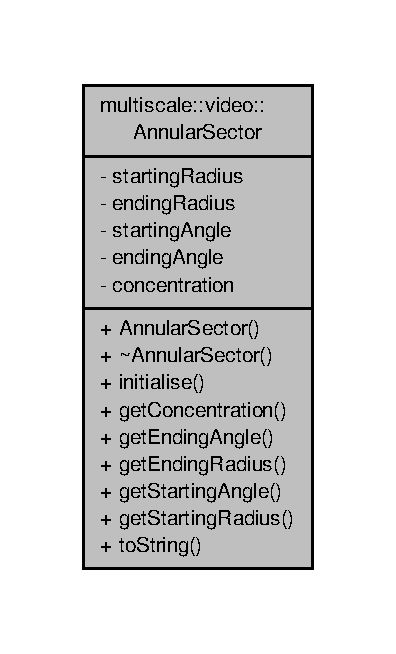
\includegraphics[width=190pt]{classmultiscale_1_1video_1_1AnnularSector__coll__graph}
\end{center}
\end{figure}
\subsection*{Public Member Functions}
\begin{DoxyCompactItemize}
\item 
\hyperlink{classmultiscale_1_1video_1_1AnnularSector_a96ea49d6d05346ef9ae99289945eb578}{Annular\-Sector} ()
\item 
\hyperlink{classmultiscale_1_1video_1_1AnnularSector_a2ced14f6af200e6e4c1c5f3e189bde4b}{$\sim$\-Annular\-Sector} ()
\item 
void \hyperlink{classmultiscale_1_1video_1_1AnnularSector_a58217c07c5c28c33f541fc37d429d79b}{initialise} (double \hyperlink{classmultiscale_1_1video_1_1AnnularSector_a4c0094d8993edb40b15580fa58a8a393}{starting\-Radius}, double \hyperlink{classmultiscale_1_1video_1_1AnnularSector_aa45c5399240707d0b3fc02ee86b97c79}{ending\-Radius}, double \hyperlink{classmultiscale_1_1video_1_1AnnularSector_a437d3dc1b2fadace28bdc3d26a78c0b3}{starting\-Angle}, double \hyperlink{classmultiscale_1_1video_1_1AnnularSector_a0aebd11072dbefe42196d6bda2e4318d}{ending\-Angle}, double \hyperlink{classmultiscale_1_1video_1_1AnnularSector_a7f6a1e7618c9e2a10e35efb5740395b1}{concentration})
\begin{DoxyCompactList}\small\item\em Initialise the members of the class. \end{DoxyCompactList}\item 
double \hyperlink{classmultiscale_1_1video_1_1AnnularSector_aee1181ae47b33a40fb2103149e45e7f1}{get\-Concentration} () const 
\begin{DoxyCompactList}\small\item\em Get the value of the concentration. \end{DoxyCompactList}\item 
double \hyperlink{classmultiscale_1_1video_1_1AnnularSector_acc074c86ca7e06ac8d5873a200498dce}{get\-Ending\-Angle} () const 
\begin{DoxyCompactList}\small\item\em Get the value of the ending angle. \end{DoxyCompactList}\item 
double \hyperlink{classmultiscale_1_1video_1_1AnnularSector_acf9600073991cf0448ab2b2997ed4513}{get\-Ending\-Radius} () const 
\begin{DoxyCompactList}\small\item\em Get the value of the ending radius. \end{DoxyCompactList}\item 
double \hyperlink{classmultiscale_1_1video_1_1AnnularSector_a85931ba16351fffc33b5a8fc714cb4b8}{get\-Starting\-Angle} () const 
\begin{DoxyCompactList}\small\item\em Get the value of the starting angle. \end{DoxyCompactList}\item 
double \hyperlink{classmultiscale_1_1video_1_1AnnularSector_aef4f23e921eae6438889f0f1537bb3ef}{get\-Starting\-Radius} () const 
\begin{DoxyCompactList}\small\item\em Get the value of the starting radius. \end{DoxyCompactList}\item 
string \hyperlink{classmultiscale_1_1video_1_1AnnularSector_ab277036c93f9dcabc08e13ca49c78e53}{to\-String} ()
\begin{DoxyCompactList}\small\item\em Get the string representation of the annular sector. \end{DoxyCompactList}\end{DoxyCompactItemize}
\subsection*{Private Attributes}
\begin{DoxyCompactItemize}
\item 
double \hyperlink{classmultiscale_1_1video_1_1AnnularSector_a4c0094d8993edb40b15580fa58a8a393}{starting\-Radius}
\item 
double \hyperlink{classmultiscale_1_1video_1_1AnnularSector_aa45c5399240707d0b3fc02ee86b97c79}{ending\-Radius}
\item 
double \hyperlink{classmultiscale_1_1video_1_1AnnularSector_a437d3dc1b2fadace28bdc3d26a78c0b3}{starting\-Angle}
\item 
double \hyperlink{classmultiscale_1_1video_1_1AnnularSector_a0aebd11072dbefe42196d6bda2e4318d}{ending\-Angle}
\item 
double \hyperlink{classmultiscale_1_1video_1_1AnnularSector_a7f6a1e7618c9e2a10e35efb5740395b1}{concentration}
\end{DoxyCompactItemize}


\subsection{Detailed Description}
An annular sector is the basic element in the considered circular geometry. 

More information about annuli and sectors of annuli can be found online (e.\-g. Wikipedia). 

Definition at line 16 of file Annular\-Sector.\-hpp.



\subsection{Constructor \& Destructor Documentation}
\hypertarget{classmultiscale_1_1video_1_1AnnularSector_a96ea49d6d05346ef9ae99289945eb578}{\index{multiscale\-::video\-::\-Annular\-Sector@{multiscale\-::video\-::\-Annular\-Sector}!Annular\-Sector@{Annular\-Sector}}
\index{Annular\-Sector@{Annular\-Sector}!multiscale::video::AnnularSector@{multiscale\-::video\-::\-Annular\-Sector}}
\subsubsection[{Annular\-Sector}]{\setlength{\rightskip}{0pt plus 5cm}Annular\-Sector\-::\-Annular\-Sector (
\begin{DoxyParamCaption}
{}
\end{DoxyParamCaption}
)}}\label{classmultiscale_1_1video_1_1AnnularSector_a96ea49d6d05346ef9ae99289945eb578}


Definition at line 11 of file Annular\-Sector.\-cpp.



References concentration, ending\-Angle, ending\-Radius, starting\-Angle, and starting\-Radius.

\hypertarget{classmultiscale_1_1video_1_1AnnularSector_a2ced14f6af200e6e4c1c5f3e189bde4b}{\index{multiscale\-::video\-::\-Annular\-Sector@{multiscale\-::video\-::\-Annular\-Sector}!$\sim$\-Annular\-Sector@{$\sim$\-Annular\-Sector}}
\index{$\sim$\-Annular\-Sector@{$\sim$\-Annular\-Sector}!multiscale::video::AnnularSector@{multiscale\-::video\-::\-Annular\-Sector}}
\subsubsection[{$\sim$\-Annular\-Sector}]{\setlength{\rightskip}{0pt plus 5cm}Annular\-Sector\-::$\sim$\-Annular\-Sector (
\begin{DoxyParamCaption}
{}
\end{DoxyParamCaption}
)}}\label{classmultiscale_1_1video_1_1AnnularSector_a2ced14f6af200e6e4c1c5f3e189bde4b}


Definition at line 19 of file Annular\-Sector.\-cpp.



\subsection{Member Function Documentation}
\hypertarget{classmultiscale_1_1video_1_1AnnularSector_aee1181ae47b33a40fb2103149e45e7f1}{\index{multiscale\-::video\-::\-Annular\-Sector@{multiscale\-::video\-::\-Annular\-Sector}!get\-Concentration@{get\-Concentration}}
\index{get\-Concentration@{get\-Concentration}!multiscale::video::AnnularSector@{multiscale\-::video\-::\-Annular\-Sector}}
\subsubsection[{get\-Concentration}]{\setlength{\rightskip}{0pt plus 5cm}double Annular\-Sector\-::get\-Concentration (
\begin{DoxyParamCaption}
{}
\end{DoxyParamCaption}
) const}}\label{classmultiscale_1_1video_1_1AnnularSector_aee1181ae47b33a40fb2103149e45e7f1}


Get the value of the concentration. 



Definition at line 30 of file Annular\-Sector.\-cpp.



References concentration.

\hypertarget{classmultiscale_1_1video_1_1AnnularSector_acc074c86ca7e06ac8d5873a200498dce}{\index{multiscale\-::video\-::\-Annular\-Sector@{multiscale\-::video\-::\-Annular\-Sector}!get\-Ending\-Angle@{get\-Ending\-Angle}}
\index{get\-Ending\-Angle@{get\-Ending\-Angle}!multiscale::video::AnnularSector@{multiscale\-::video\-::\-Annular\-Sector}}
\subsubsection[{get\-Ending\-Angle}]{\setlength{\rightskip}{0pt plus 5cm}double Annular\-Sector\-::get\-Ending\-Angle (
\begin{DoxyParamCaption}
{}
\end{DoxyParamCaption}
) const}}\label{classmultiscale_1_1video_1_1AnnularSector_acc074c86ca7e06ac8d5873a200498dce}


Get the value of the ending angle. 



Definition at line 34 of file Annular\-Sector.\-cpp.



References ending\-Angle.

\hypertarget{classmultiscale_1_1video_1_1AnnularSector_acf9600073991cf0448ab2b2997ed4513}{\index{multiscale\-::video\-::\-Annular\-Sector@{multiscale\-::video\-::\-Annular\-Sector}!get\-Ending\-Radius@{get\-Ending\-Radius}}
\index{get\-Ending\-Radius@{get\-Ending\-Radius}!multiscale::video::AnnularSector@{multiscale\-::video\-::\-Annular\-Sector}}
\subsubsection[{get\-Ending\-Radius}]{\setlength{\rightskip}{0pt plus 5cm}double Annular\-Sector\-::get\-Ending\-Radius (
\begin{DoxyParamCaption}
{}
\end{DoxyParamCaption}
) const}}\label{classmultiscale_1_1video_1_1AnnularSector_acf9600073991cf0448ab2b2997ed4513}


Get the value of the ending radius. 



Definition at line 38 of file Annular\-Sector.\-cpp.



References ending\-Radius.

\hypertarget{classmultiscale_1_1video_1_1AnnularSector_a85931ba16351fffc33b5a8fc714cb4b8}{\index{multiscale\-::video\-::\-Annular\-Sector@{multiscale\-::video\-::\-Annular\-Sector}!get\-Starting\-Angle@{get\-Starting\-Angle}}
\index{get\-Starting\-Angle@{get\-Starting\-Angle}!multiscale::video::AnnularSector@{multiscale\-::video\-::\-Annular\-Sector}}
\subsubsection[{get\-Starting\-Angle}]{\setlength{\rightskip}{0pt plus 5cm}double Annular\-Sector\-::get\-Starting\-Angle (
\begin{DoxyParamCaption}
{}
\end{DoxyParamCaption}
) const}}\label{classmultiscale_1_1video_1_1AnnularSector_a85931ba16351fffc33b5a8fc714cb4b8}


Get the value of the starting angle. 



Definition at line 42 of file Annular\-Sector.\-cpp.



References starting\-Angle.

\hypertarget{classmultiscale_1_1video_1_1AnnularSector_aef4f23e921eae6438889f0f1537bb3ef}{\index{multiscale\-::video\-::\-Annular\-Sector@{multiscale\-::video\-::\-Annular\-Sector}!get\-Starting\-Radius@{get\-Starting\-Radius}}
\index{get\-Starting\-Radius@{get\-Starting\-Radius}!multiscale::video::AnnularSector@{multiscale\-::video\-::\-Annular\-Sector}}
\subsubsection[{get\-Starting\-Radius}]{\setlength{\rightskip}{0pt plus 5cm}double Annular\-Sector\-::get\-Starting\-Radius (
\begin{DoxyParamCaption}
{}
\end{DoxyParamCaption}
) const}}\label{classmultiscale_1_1video_1_1AnnularSector_aef4f23e921eae6438889f0f1537bb3ef}


Get the value of the starting radius. 



Definition at line 46 of file Annular\-Sector.\-cpp.



References starting\-Radius.

\hypertarget{classmultiscale_1_1video_1_1AnnularSector_a58217c07c5c28c33f541fc37d429d79b}{\index{multiscale\-::video\-::\-Annular\-Sector@{multiscale\-::video\-::\-Annular\-Sector}!initialise@{initialise}}
\index{initialise@{initialise}!multiscale::video::AnnularSector@{multiscale\-::video\-::\-Annular\-Sector}}
\subsubsection[{initialise}]{\setlength{\rightskip}{0pt plus 5cm}void Annular\-Sector\-::initialise (
\begin{DoxyParamCaption}
\item[{double}]{starting\-Radius, }
\item[{double}]{ending\-Radius, }
\item[{double}]{starting\-Angle, }
\item[{double}]{ending\-Angle, }
\item[{double}]{concentration}
\end{DoxyParamCaption}
)}}\label{classmultiscale_1_1video_1_1AnnularSector_a58217c07c5c28c33f541fc37d429d79b}


Initialise the members of the class. 


\begin{DoxyParams}{Parameters}
{\em starting\-Radius} & Starting radius \\
\hline
{\em ending\-Radius} & Ending radius \\
\hline
{\em starting\-Angle} & Starting angle \\
\hline
{\em ending\-Angle} & Ending angle \\
\hline
{\em concentration} & Concentration \\
\hline
\end{DoxyParams}


Definition at line 21 of file Annular\-Sector.\-cpp.



References concentration, ending\-Angle, ending\-Radius, starting\-Angle, and starting\-Radius.

\hypertarget{classmultiscale_1_1video_1_1AnnularSector_ab277036c93f9dcabc08e13ca49c78e53}{\index{multiscale\-::video\-::\-Annular\-Sector@{multiscale\-::video\-::\-Annular\-Sector}!to\-String@{to\-String}}
\index{to\-String@{to\-String}!multiscale::video::AnnularSector@{multiscale\-::video\-::\-Annular\-Sector}}
\subsubsection[{to\-String}]{\setlength{\rightskip}{0pt plus 5cm}string Annular\-Sector\-::to\-String (
\begin{DoxyParamCaption}
{}
\end{DoxyParamCaption}
)}}\label{classmultiscale_1_1video_1_1AnnularSector_ab277036c93f9dcabc08e13ca49c78e53}


Get the string representation of the annular sector. 



Definition at line 50 of file Annular\-Sector.\-cpp.



References concentration, ending\-Angle, ending\-Radius, S\-E\-P\-A\-R\-A\-T\-O\-R, starting\-Angle, and starting\-Radius.



\subsection{Member Data Documentation}
\hypertarget{classmultiscale_1_1video_1_1AnnularSector_a7f6a1e7618c9e2a10e35efb5740395b1}{\index{multiscale\-::video\-::\-Annular\-Sector@{multiscale\-::video\-::\-Annular\-Sector}!concentration@{concentration}}
\index{concentration@{concentration}!multiscale::video::AnnularSector@{multiscale\-::video\-::\-Annular\-Sector}}
\subsubsection[{concentration}]{\setlength{\rightskip}{0pt plus 5cm}double multiscale\-::video\-::\-Annular\-Sector\-::concentration\hspace{0.3cm}{\ttfamily [private]}}}\label{classmultiscale_1_1video_1_1AnnularSector_a7f6a1e7618c9e2a10e35efb5740395b1}


Definition at line 24 of file Annular\-Sector.\-hpp.



Referenced by Annular\-Sector(), get\-Concentration(), initialise(), and to\-String().

\hypertarget{classmultiscale_1_1video_1_1AnnularSector_a0aebd11072dbefe42196d6bda2e4318d}{\index{multiscale\-::video\-::\-Annular\-Sector@{multiscale\-::video\-::\-Annular\-Sector}!ending\-Angle@{ending\-Angle}}
\index{ending\-Angle@{ending\-Angle}!multiscale::video::AnnularSector@{multiscale\-::video\-::\-Annular\-Sector}}
\subsubsection[{ending\-Angle}]{\setlength{\rightskip}{0pt plus 5cm}double multiscale\-::video\-::\-Annular\-Sector\-::ending\-Angle\hspace{0.3cm}{\ttfamily [private]}}}\label{classmultiscale_1_1video_1_1AnnularSector_a0aebd11072dbefe42196d6bda2e4318d}


Definition at line 23 of file Annular\-Sector.\-hpp.



Referenced by Annular\-Sector(), get\-Ending\-Angle(), initialise(), and to\-String().

\hypertarget{classmultiscale_1_1video_1_1AnnularSector_aa45c5399240707d0b3fc02ee86b97c79}{\index{multiscale\-::video\-::\-Annular\-Sector@{multiscale\-::video\-::\-Annular\-Sector}!ending\-Radius@{ending\-Radius}}
\index{ending\-Radius@{ending\-Radius}!multiscale::video::AnnularSector@{multiscale\-::video\-::\-Annular\-Sector}}
\subsubsection[{ending\-Radius}]{\setlength{\rightskip}{0pt plus 5cm}double multiscale\-::video\-::\-Annular\-Sector\-::ending\-Radius\hspace{0.3cm}{\ttfamily [private]}}}\label{classmultiscale_1_1video_1_1AnnularSector_aa45c5399240707d0b3fc02ee86b97c79}


Definition at line 21 of file Annular\-Sector.\-hpp.



Referenced by Annular\-Sector(), get\-Ending\-Radius(), initialise(), and to\-String().

\hypertarget{classmultiscale_1_1video_1_1AnnularSector_a437d3dc1b2fadace28bdc3d26a78c0b3}{\index{multiscale\-::video\-::\-Annular\-Sector@{multiscale\-::video\-::\-Annular\-Sector}!starting\-Angle@{starting\-Angle}}
\index{starting\-Angle@{starting\-Angle}!multiscale::video::AnnularSector@{multiscale\-::video\-::\-Annular\-Sector}}
\subsubsection[{starting\-Angle}]{\setlength{\rightskip}{0pt plus 5cm}double multiscale\-::video\-::\-Annular\-Sector\-::starting\-Angle\hspace{0.3cm}{\ttfamily [private]}}}\label{classmultiscale_1_1video_1_1AnnularSector_a437d3dc1b2fadace28bdc3d26a78c0b3}


Definition at line 22 of file Annular\-Sector.\-hpp.



Referenced by Annular\-Sector(), get\-Starting\-Angle(), initialise(), and to\-String().

\hypertarget{classmultiscale_1_1video_1_1AnnularSector_a4c0094d8993edb40b15580fa58a8a393}{\index{multiscale\-::video\-::\-Annular\-Sector@{multiscale\-::video\-::\-Annular\-Sector}!starting\-Radius@{starting\-Radius}}
\index{starting\-Radius@{starting\-Radius}!multiscale::video::AnnularSector@{multiscale\-::video\-::\-Annular\-Sector}}
\subsubsection[{starting\-Radius}]{\setlength{\rightskip}{0pt plus 5cm}double multiscale\-::video\-::\-Annular\-Sector\-::starting\-Radius\hspace{0.3cm}{\ttfamily [private]}}}\label{classmultiscale_1_1video_1_1AnnularSector_a4c0094d8993edb40b15580fa58a8a393}


Definition at line 20 of file Annular\-Sector.\-hpp.



Referenced by Annular\-Sector(), get\-Starting\-Radius(), initialise(), and to\-String().



The documentation for this class was generated from the following files\-:\begin{DoxyCompactItemize}
\item 
/home/ovidiu/\-Repositories/git/multiscale/\-Multiscale/modules/video/circular/include/multiscale/video/circular/\hyperlink{AnnularSector_8hpp}{Annular\-Sector.\-hpp}\item 
/home/ovidiu/\-Repositories/git/multiscale/\-Multiscale/modules/video/circular/src/\hyperlink{AnnularSector_8cpp}{Annular\-Sector.\-cpp}\end{DoxyCompactItemize}

\hypertarget{classmultiscale_1_1video_1_1CartesianToConcentrationsConverter}{\section{multiscale\-:\-:video\-:\-:Cartesian\-To\-Concentrations\-Converter Class Reference}
\label{classmultiscale_1_1video_1_1CartesianToConcentrationsConverter}\index{multiscale\-::video\-::\-Cartesian\-To\-Concentrations\-Converter@{multiscale\-::video\-::\-Cartesian\-To\-Concentrations\-Converter}}
}


Scale the values of the rectangular geometry grid cells.  




{\ttfamily \#include $<$Cartesian\-To\-Concentrations\-Converter.\-hpp$>$}



Collaboration diagram for multiscale\-:\-:video\-:\-:Cartesian\-To\-Concentrations\-Converter\-:\nopagebreak
\begin{figure}[H]
\begin{center}
\leavevmode
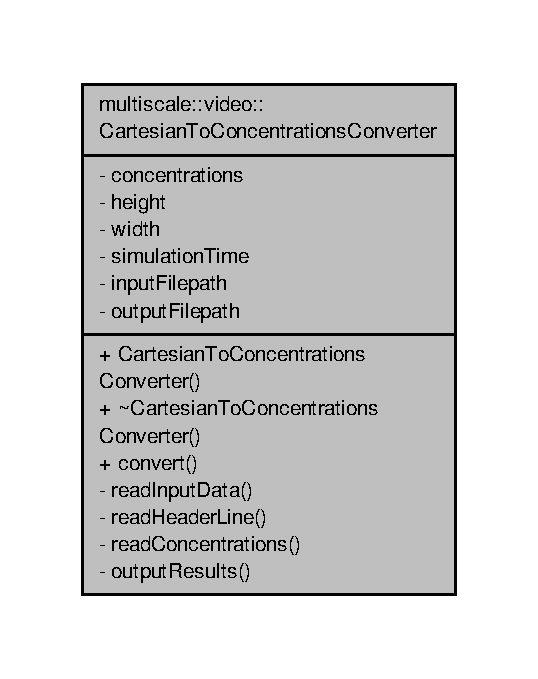
\includegraphics[width=258pt]{classmultiscale_1_1video_1_1CartesianToConcentrationsConverter__coll__graph}
\end{center}
\end{figure}
\subsection*{Public Member Functions}
\begin{DoxyCompactItemize}
\item 
\hyperlink{classmultiscale_1_1video_1_1CartesianToConcentrationsConverter_ae2f641fe6c2af730a5aedc83f4bc1244}{Cartesian\-To\-Concentrations\-Converter} (const string \&\hyperlink{classmultiscale_1_1video_1_1CartesianToConcentrationsConverter_affebbc7e1c67692bd529f19fc0451e58}{input\-Filepath}, const string \&\hyperlink{classmultiscale_1_1video_1_1CartesianToConcentrationsConverter_a9215448e33876a581b206a89b6651fd0}{output\-Filepath})
\item 
\hyperlink{classmultiscale_1_1video_1_1CartesianToConcentrationsConverter_a4250cb00af6f3c254c0577479ae25553}{$\sim$\-Cartesian\-To\-Concentrations\-Converter} ()
\item 
void \hyperlink{classmultiscale_1_1video_1_1CartesianToConcentrationsConverter_a27de97c7e35097bd17453fd07f33a6f1}{convert} ()
\begin{DoxyCompactList}\small\item\em Start the conversion. \end{DoxyCompactList}\end{DoxyCompactItemize}
\subsection*{Private Member Functions}
\begin{DoxyCompactItemize}
\item 
void \hyperlink{classmultiscale_1_1video_1_1CartesianToConcentrationsConverter_a94094cdeaf0f48164911188709dc0e2f}{read\-Input\-Data} ()
\begin{DoxyCompactList}\small\item\em Read the input data. \end{DoxyCompactList}\item 
void \hyperlink{classmultiscale_1_1video_1_1CartesianToConcentrationsConverter_a2e9967ae6fb2efc39ed377aca2fa222c}{read\-Header\-Line} (ifstream \&fin)
\begin{DoxyCompactList}\small\item\em Read the header line. \end{DoxyCompactList}\item 
void \hyperlink{classmultiscale_1_1video_1_1CartesianToConcentrationsConverter_a9134409b814fafe62c896c6b473bc574}{read\-Concentrations} (ifstream \&fin)
\begin{DoxyCompactList}\small\item\em Read the concentrations. \end{DoxyCompactList}\item 
void \hyperlink{classmultiscale_1_1video_1_1CartesianToConcentrationsConverter_a346e054266585ae6922d159b8d5fb804}{output\-Results} ()
\begin{DoxyCompactList}\small\item\em Output the results. \end{DoxyCompactList}\end{DoxyCompactItemize}
\subsection*{Private Attributes}
\begin{DoxyCompactItemize}
\item 
vector$<$ double $>$ \hyperlink{classmultiscale_1_1video_1_1CartesianToConcentrationsConverter_a335f54163cbabeaa80c1da811b9f9c0c}{concentrations}
\item 
unsigned long \hyperlink{classmultiscale_1_1video_1_1CartesianToConcentrationsConverter_a94e58072f2e143bd6476133370ffb37f}{height}
\item 
unsigned long \hyperlink{classmultiscale_1_1video_1_1CartesianToConcentrationsConverter_ae6fba5af405d884c7b70ed206a6d5cb1}{width}
\item 
double \hyperlink{classmultiscale_1_1video_1_1CartesianToConcentrationsConverter_a6e66af60b82513b3186fdb32cad44597}{simulation\-Time}
\item 
string \hyperlink{classmultiscale_1_1video_1_1CartesianToConcentrationsConverter_affebbc7e1c67692bd529f19fc0451e58}{input\-Filepath}
\item 
string \hyperlink{classmultiscale_1_1video_1_1CartesianToConcentrationsConverter_a9215448e33876a581b206a89b6651fd0}{output\-Filepath}
\end{DoxyCompactItemize}


\subsection{Detailed Description}
Scale the values of the rectangular geometry grid cells. 

Definition at line 26 of file Cartesian\-To\-Concentrations\-Converter.\-hpp.



\subsection{Constructor \& Destructor Documentation}
\hypertarget{classmultiscale_1_1video_1_1CartesianToConcentrationsConverter_ae2f641fe6c2af730a5aedc83f4bc1244}{\index{multiscale\-::video\-::\-Cartesian\-To\-Concentrations\-Converter@{multiscale\-::video\-::\-Cartesian\-To\-Concentrations\-Converter}!Cartesian\-To\-Concentrations\-Converter@{Cartesian\-To\-Concentrations\-Converter}}
\index{Cartesian\-To\-Concentrations\-Converter@{Cartesian\-To\-Concentrations\-Converter}!multiscale::video::CartesianToConcentrationsConverter@{multiscale\-::video\-::\-Cartesian\-To\-Concentrations\-Converter}}
\subsubsection[{Cartesian\-To\-Concentrations\-Converter}]{\setlength{\rightskip}{0pt plus 5cm}Cartesian\-To\-Concentrations\-Converter\-::\-Cartesian\-To\-Concentrations\-Converter (
\begin{DoxyParamCaption}
\item[{const string \&}]{input\-Filepath, }
\item[{const string \&}]{output\-Filepath}
\end{DoxyParamCaption}
)}}\label{classmultiscale_1_1video_1_1CartesianToConcentrationsConverter_ae2f641fe6c2af730a5aedc83f4bc1244}


Definition at line 15 of file Cartesian\-To\-Concentrations\-Converter.\-cpp.



References height, simulation\-Time, and width.

\hypertarget{classmultiscale_1_1video_1_1CartesianToConcentrationsConverter_a4250cb00af6f3c254c0577479ae25553}{\index{multiscale\-::video\-::\-Cartesian\-To\-Concentrations\-Converter@{multiscale\-::video\-::\-Cartesian\-To\-Concentrations\-Converter}!$\sim$\-Cartesian\-To\-Concentrations\-Converter@{$\sim$\-Cartesian\-To\-Concentrations\-Converter}}
\index{$\sim$\-Cartesian\-To\-Concentrations\-Converter@{$\sim$\-Cartesian\-To\-Concentrations\-Converter}!multiscale::video::CartesianToConcentrationsConverter@{multiscale\-::video\-::\-Cartesian\-To\-Concentrations\-Converter}}
\subsubsection[{$\sim$\-Cartesian\-To\-Concentrations\-Converter}]{\setlength{\rightskip}{0pt plus 5cm}Cartesian\-To\-Concentrations\-Converter\-::$\sim$\-Cartesian\-To\-Concentrations\-Converter (
\begin{DoxyParamCaption}
{}
\end{DoxyParamCaption}
)}}\label{classmultiscale_1_1video_1_1CartesianToConcentrationsConverter_a4250cb00af6f3c254c0577479ae25553}


Definition at line 24 of file Cartesian\-To\-Concentrations\-Converter.\-cpp.



\subsection{Member Function Documentation}
\hypertarget{classmultiscale_1_1video_1_1CartesianToConcentrationsConverter_a27de97c7e35097bd17453fd07f33a6f1}{\index{multiscale\-::video\-::\-Cartesian\-To\-Concentrations\-Converter@{multiscale\-::video\-::\-Cartesian\-To\-Concentrations\-Converter}!convert@{convert}}
\index{convert@{convert}!multiscale::video::CartesianToConcentrationsConverter@{multiscale\-::video\-::\-Cartesian\-To\-Concentrations\-Converter}}
\subsubsection[{convert}]{\setlength{\rightskip}{0pt plus 5cm}void Cartesian\-To\-Concentrations\-Converter\-::convert (
\begin{DoxyParamCaption}
{}
\end{DoxyParamCaption}
)}}\label{classmultiscale_1_1video_1_1CartesianToConcentrationsConverter_a27de97c7e35097bd17453fd07f33a6f1}


Start the conversion. 



Definition at line 26 of file Cartesian\-To\-Concentrations\-Converter.\-cpp.



References output\-Results(), and read\-Input\-Data().



Referenced by main().



Here is the call graph for this function\-:\nopagebreak
\begin{figure}[H]
\begin{center}
\leavevmode
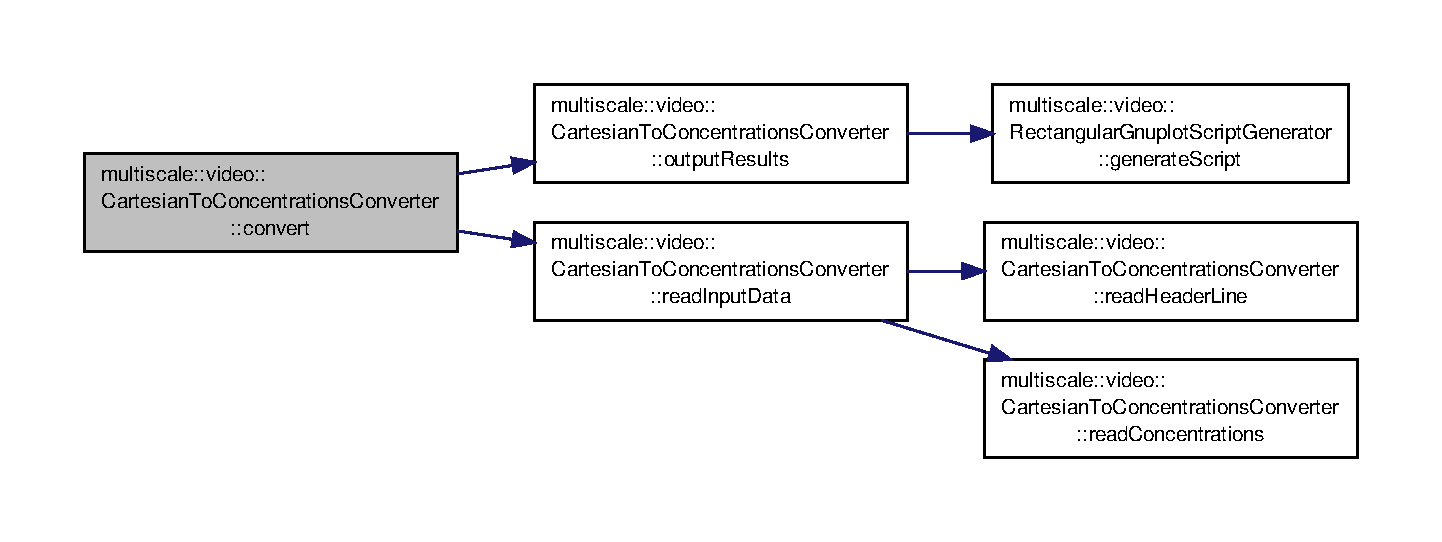
\includegraphics[width=350pt]{classmultiscale_1_1video_1_1CartesianToConcentrationsConverter_a27de97c7e35097bd17453fd07f33a6f1_cgraph}
\end{center}
\end{figure}




Here is the caller graph for this function\-:\nopagebreak
\begin{figure}[H]
\begin{center}
\leavevmode
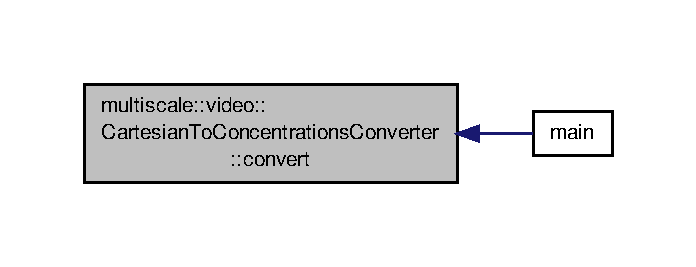
\includegraphics[width=334pt]{classmultiscale_1_1video_1_1CartesianToConcentrationsConverter_a27de97c7e35097bd17453fd07f33a6f1_icgraph}
\end{center}
\end{figure}


\hypertarget{classmultiscale_1_1video_1_1CartesianToConcentrationsConverter_a346e054266585ae6922d159b8d5fb804}{\index{multiscale\-::video\-::\-Cartesian\-To\-Concentrations\-Converter@{multiscale\-::video\-::\-Cartesian\-To\-Concentrations\-Converter}!output\-Results@{output\-Results}}
\index{output\-Results@{output\-Results}!multiscale::video::CartesianToConcentrationsConverter@{multiscale\-::video\-::\-Cartesian\-To\-Concentrations\-Converter}}
\subsubsection[{output\-Results}]{\setlength{\rightskip}{0pt plus 5cm}void Cartesian\-To\-Concentrations\-Converter\-::output\-Results (
\begin{DoxyParamCaption}
{}
\end{DoxyParamCaption}
)\hspace{0.3cm}{\ttfamily [private]}}}\label{classmultiscale_1_1video_1_1CartesianToConcentrationsConverter_a346e054266585ae6922d159b8d5fb804}


Output the results. 



Definition at line 84 of file Cartesian\-To\-Concentrations\-Converter.\-cpp.



References concentrations, multiscale\-::video\-::\-Rectangular\-Gnuplot\-Script\-Generator\-::generate\-Script(), height, output\-Filepath, simulation\-Time, and width.



Referenced by convert().



Here is the call graph for this function\-:\nopagebreak
\begin{figure}[H]
\begin{center}
\leavevmode
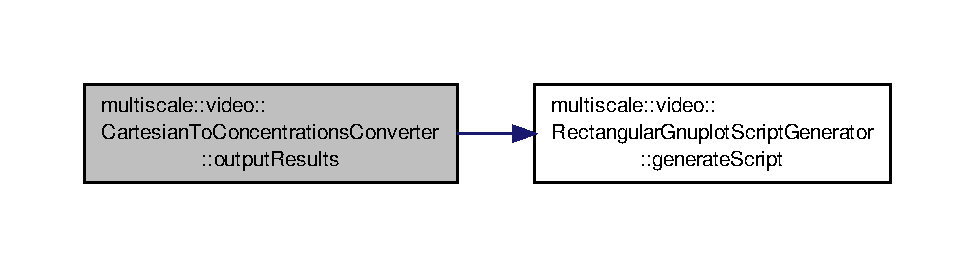
\includegraphics[width=350pt]{classmultiscale_1_1video_1_1CartesianToConcentrationsConverter_a346e054266585ae6922d159b8d5fb804_cgraph}
\end{center}
\end{figure}




Here is the caller graph for this function\-:\nopagebreak
\begin{figure}[H]
\begin{center}
\leavevmode
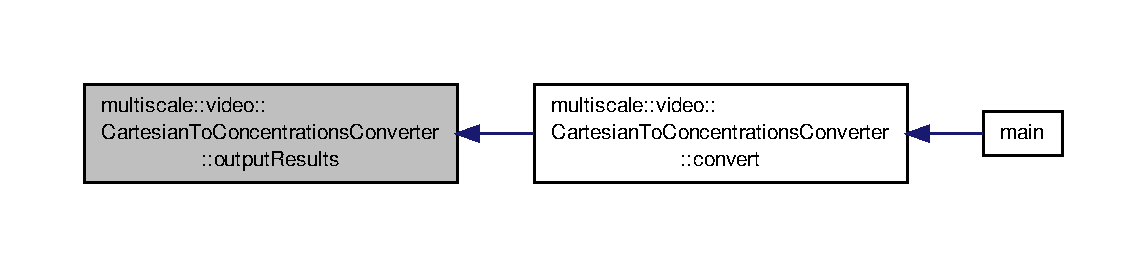
\includegraphics[width=350pt]{classmultiscale_1_1video_1_1CartesianToConcentrationsConverter_a346e054266585ae6922d159b8d5fb804_icgraph}
\end{center}
\end{figure}


\hypertarget{classmultiscale_1_1video_1_1CartesianToConcentrationsConverter_a9134409b814fafe62c896c6b473bc574}{\index{multiscale\-::video\-::\-Cartesian\-To\-Concentrations\-Converter@{multiscale\-::video\-::\-Cartesian\-To\-Concentrations\-Converter}!read\-Concentrations@{read\-Concentrations}}
\index{read\-Concentrations@{read\-Concentrations}!multiscale::video::CartesianToConcentrationsConverter@{multiscale\-::video\-::\-Cartesian\-To\-Concentrations\-Converter}}
\subsubsection[{read\-Concentrations}]{\setlength{\rightskip}{0pt plus 5cm}void Cartesian\-To\-Concentrations\-Converter\-::read\-Concentrations (
\begin{DoxyParamCaption}
\item[{ifstream \&}]{fin}
\end{DoxyParamCaption}
)\hspace{0.3cm}{\ttfamily [private]}}}\label{classmultiscale_1_1video_1_1CartesianToConcentrationsConverter_a9134409b814fafe62c896c6b473bc574}


Read the concentrations. 


\begin{DoxyParams}{Parameters}
{\em fin} & Input file stream \\
\hline
\end{DoxyParams}


Definition at line 64 of file Cartesian\-To\-Concentrations\-Converter.\-cpp.



References concentrations, E\-R\-R\-\_\-\-C\-O\-N\-C, height, and width.



Referenced by read\-Input\-Data().



Here is the caller graph for this function\-:\nopagebreak
\begin{figure}[H]
\begin{center}
\leavevmode
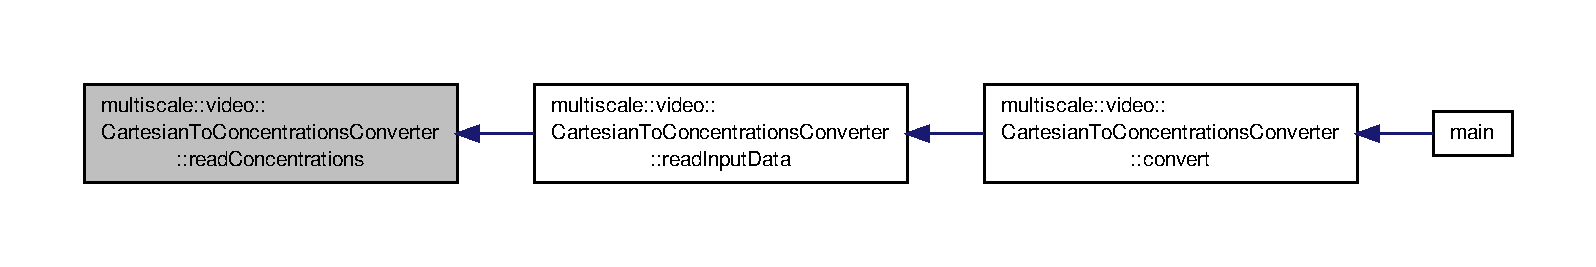
\includegraphics[width=350pt]{classmultiscale_1_1video_1_1CartesianToConcentrationsConverter_a9134409b814fafe62c896c6b473bc574_icgraph}
\end{center}
\end{figure}


\hypertarget{classmultiscale_1_1video_1_1CartesianToConcentrationsConverter_a2e9967ae6fb2efc39ed377aca2fa222c}{\index{multiscale\-::video\-::\-Cartesian\-To\-Concentrations\-Converter@{multiscale\-::video\-::\-Cartesian\-To\-Concentrations\-Converter}!read\-Header\-Line@{read\-Header\-Line}}
\index{read\-Header\-Line@{read\-Header\-Line}!multiscale::video::CartesianToConcentrationsConverter@{multiscale\-::video\-::\-Cartesian\-To\-Concentrations\-Converter}}
\subsubsection[{read\-Header\-Line}]{\setlength{\rightskip}{0pt plus 5cm}void Cartesian\-To\-Concentrations\-Converter\-::read\-Header\-Line (
\begin{DoxyParamCaption}
\item[{ifstream \&}]{fin}
\end{DoxyParamCaption}
)\hspace{0.3cm}{\ttfamily [private]}}}\label{classmultiscale_1_1video_1_1CartesianToConcentrationsConverter_a2e9967ae6fb2efc39ed377aca2fa222c}


Read the header line. 

The header line contains values for number of concentric circles, number of sectors and simulation time


\begin{DoxyParams}{Parameters}
{\em fin} & Input file stream \\
\hline
\end{DoxyParams}


Definition at line 55 of file Cartesian\-To\-Concentrations\-Converter.\-cpp.



References E\-R\-R\-\_\-\-N\-E\-G\-\_\-\-S\-I\-M\-\_\-\-T\-I\-M\-E, E\-R\-R\-\_\-\-N\-O\-N\-P\-O\-S\-\_\-\-D\-I\-M\-E\-N\-S\-I\-O\-N, height, simulation\-Time, and width.



Referenced by read\-Input\-Data().



Here is the caller graph for this function\-:\nopagebreak
\begin{figure}[H]
\begin{center}
\leavevmode
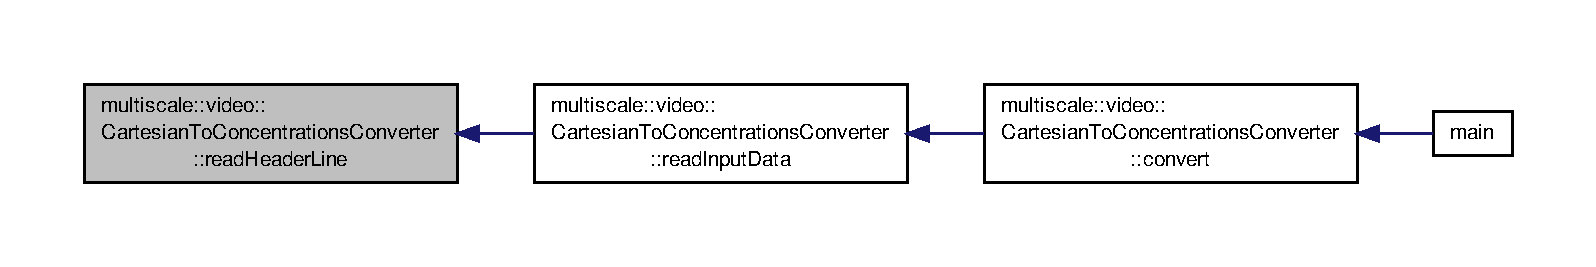
\includegraphics[width=350pt]{classmultiscale_1_1video_1_1CartesianToConcentrationsConverter_a2e9967ae6fb2efc39ed377aca2fa222c_icgraph}
\end{center}
\end{figure}


\hypertarget{classmultiscale_1_1video_1_1CartesianToConcentrationsConverter_a94094cdeaf0f48164911188709dc0e2f}{\index{multiscale\-::video\-::\-Cartesian\-To\-Concentrations\-Converter@{multiscale\-::video\-::\-Cartesian\-To\-Concentrations\-Converter}!read\-Input\-Data@{read\-Input\-Data}}
\index{read\-Input\-Data@{read\-Input\-Data}!multiscale::video::CartesianToConcentrationsConverter@{multiscale\-::video\-::\-Cartesian\-To\-Concentrations\-Converter}}
\subsubsection[{read\-Input\-Data}]{\setlength{\rightskip}{0pt plus 5cm}void Cartesian\-To\-Concentrations\-Converter\-::read\-Input\-Data (
\begin{DoxyParamCaption}
{}
\end{DoxyParamCaption}
)\hspace{0.3cm}{\ttfamily [private]}}}\label{classmultiscale_1_1video_1_1CartesianToConcentrationsConverter_a94094cdeaf0f48164911188709dc0e2f}


Read the input data. 



Definition at line 31 of file Cartesian\-To\-Concentrations\-Converter.\-cpp.



References E\-R\-R\-\_\-\-I\-N\-\_\-\-E\-X\-T\-R\-A\-\_\-\-D\-A\-T\-A, E\-R\-R\-\_\-\-I\-N\-P\-U\-T\-\_\-\-O\-P\-E\-N, input\-Filepath, read\-Concentrations(), and read\-Header\-Line().



Referenced by convert().



Here is the call graph for this function\-:\nopagebreak
\begin{figure}[H]
\begin{center}
\leavevmode
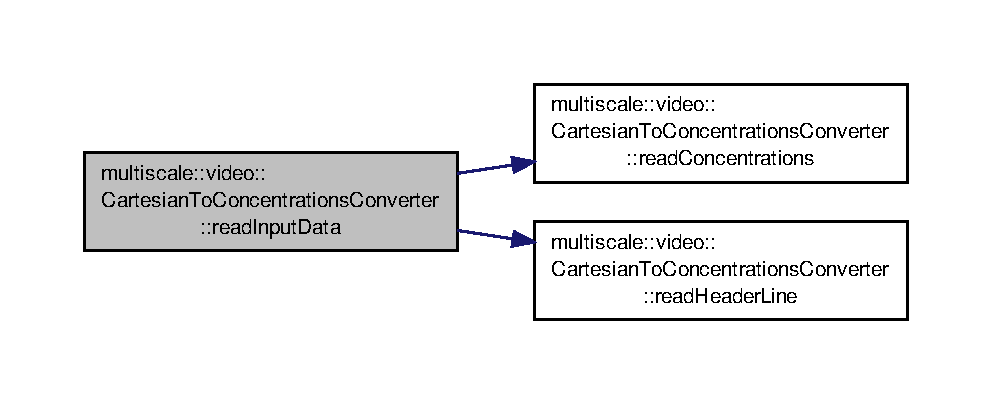
\includegraphics[width=350pt]{classmultiscale_1_1video_1_1CartesianToConcentrationsConverter_a94094cdeaf0f48164911188709dc0e2f_cgraph}
\end{center}
\end{figure}




Here is the caller graph for this function\-:\nopagebreak
\begin{figure}[H]
\begin{center}
\leavevmode
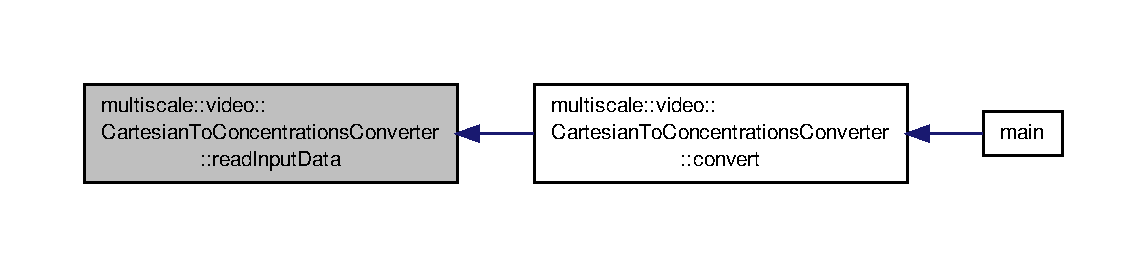
\includegraphics[width=350pt]{classmultiscale_1_1video_1_1CartesianToConcentrationsConverter_a94094cdeaf0f48164911188709dc0e2f_icgraph}
\end{center}
\end{figure}




\subsection{Member Data Documentation}
\hypertarget{classmultiscale_1_1video_1_1CartesianToConcentrationsConverter_a335f54163cbabeaa80c1da811b9f9c0c}{\index{multiscale\-::video\-::\-Cartesian\-To\-Concentrations\-Converter@{multiscale\-::video\-::\-Cartesian\-To\-Concentrations\-Converter}!concentrations@{concentrations}}
\index{concentrations@{concentrations}!multiscale::video::CartesianToConcentrationsConverter@{multiscale\-::video\-::\-Cartesian\-To\-Concentrations\-Converter}}
\subsubsection[{concentrations}]{\setlength{\rightskip}{0pt plus 5cm}vector$<$double$>$ multiscale\-::video\-::\-Cartesian\-To\-Concentrations\-Converter\-::concentrations\hspace{0.3cm}{\ttfamily [private]}}}\label{classmultiscale_1_1video_1_1CartesianToConcentrationsConverter_a335f54163cbabeaa80c1da811b9f9c0c}
Concentrations received as input 

Definition at line 30 of file Cartesian\-To\-Concentrations\-Converter.\-hpp.



Referenced by output\-Results(), and read\-Concentrations().

\hypertarget{classmultiscale_1_1video_1_1CartesianToConcentrationsConverter_a94e58072f2e143bd6476133370ffb37f}{\index{multiscale\-::video\-::\-Cartesian\-To\-Concentrations\-Converter@{multiscale\-::video\-::\-Cartesian\-To\-Concentrations\-Converter}!height@{height}}
\index{height@{height}!multiscale::video::CartesianToConcentrationsConverter@{multiscale\-::video\-::\-Cartesian\-To\-Concentrations\-Converter}}
\subsubsection[{height}]{\setlength{\rightskip}{0pt plus 5cm}unsigned long multiscale\-::video\-::\-Cartesian\-To\-Concentrations\-Converter\-::height\hspace{0.3cm}{\ttfamily [private]}}}\label{classmultiscale_1_1video_1_1CartesianToConcentrationsConverter_a94e58072f2e143bd6476133370ffb37f}
Height of the grid 

Definition at line 32 of file Cartesian\-To\-Concentrations\-Converter.\-hpp.



Referenced by Cartesian\-To\-Concentrations\-Converter(), output\-Results(), read\-Concentrations(), and read\-Header\-Line().

\hypertarget{classmultiscale_1_1video_1_1CartesianToConcentrationsConverter_affebbc7e1c67692bd529f19fc0451e58}{\index{multiscale\-::video\-::\-Cartesian\-To\-Concentrations\-Converter@{multiscale\-::video\-::\-Cartesian\-To\-Concentrations\-Converter}!input\-Filepath@{input\-Filepath}}
\index{input\-Filepath@{input\-Filepath}!multiscale::video::CartesianToConcentrationsConverter@{multiscale\-::video\-::\-Cartesian\-To\-Concentrations\-Converter}}
\subsubsection[{input\-Filepath}]{\setlength{\rightskip}{0pt plus 5cm}string multiscale\-::video\-::\-Cartesian\-To\-Concentrations\-Converter\-::input\-Filepath\hspace{0.3cm}{\ttfamily [private]}}}\label{classmultiscale_1_1video_1_1CartesianToConcentrationsConverter_affebbc7e1c67692bd529f19fc0451e58}
Path to the input file 

Definition at line 36 of file Cartesian\-To\-Concentrations\-Converter.\-hpp.



Referenced by read\-Input\-Data().

\hypertarget{classmultiscale_1_1video_1_1CartesianToConcentrationsConverter_a9215448e33876a581b206a89b6651fd0}{\index{multiscale\-::video\-::\-Cartesian\-To\-Concentrations\-Converter@{multiscale\-::video\-::\-Cartesian\-To\-Concentrations\-Converter}!output\-Filepath@{output\-Filepath}}
\index{output\-Filepath@{output\-Filepath}!multiscale::video::CartesianToConcentrationsConverter@{multiscale\-::video\-::\-Cartesian\-To\-Concentrations\-Converter}}
\subsubsection[{output\-Filepath}]{\setlength{\rightskip}{0pt plus 5cm}string multiscale\-::video\-::\-Cartesian\-To\-Concentrations\-Converter\-::output\-Filepath\hspace{0.3cm}{\ttfamily [private]}}}\label{classmultiscale_1_1video_1_1CartesianToConcentrationsConverter_a9215448e33876a581b206a89b6651fd0}
Path to the output file 

Definition at line 37 of file Cartesian\-To\-Concentrations\-Converter.\-hpp.



Referenced by output\-Results().

\hypertarget{classmultiscale_1_1video_1_1CartesianToConcentrationsConverter_a6e66af60b82513b3186fdb32cad44597}{\index{multiscale\-::video\-::\-Cartesian\-To\-Concentrations\-Converter@{multiscale\-::video\-::\-Cartesian\-To\-Concentrations\-Converter}!simulation\-Time@{simulation\-Time}}
\index{simulation\-Time@{simulation\-Time}!multiscale::video::CartesianToConcentrationsConverter@{multiscale\-::video\-::\-Cartesian\-To\-Concentrations\-Converter}}
\subsubsection[{simulation\-Time}]{\setlength{\rightskip}{0pt plus 5cm}double multiscale\-::video\-::\-Cartesian\-To\-Concentrations\-Converter\-::simulation\-Time\hspace{0.3cm}{\ttfamily [private]}}}\label{classmultiscale_1_1video_1_1CartesianToConcentrationsConverter_a6e66af60b82513b3186fdb32cad44597}
Simulation time 

Definition at line 34 of file Cartesian\-To\-Concentrations\-Converter.\-hpp.



Referenced by Cartesian\-To\-Concentrations\-Converter(), output\-Results(), and read\-Header\-Line().

\hypertarget{classmultiscale_1_1video_1_1CartesianToConcentrationsConverter_ae6fba5af405d884c7b70ed206a6d5cb1}{\index{multiscale\-::video\-::\-Cartesian\-To\-Concentrations\-Converter@{multiscale\-::video\-::\-Cartesian\-To\-Concentrations\-Converter}!width@{width}}
\index{width@{width}!multiscale::video::CartesianToConcentrationsConverter@{multiscale\-::video\-::\-Cartesian\-To\-Concentrations\-Converter}}
\subsubsection[{width}]{\setlength{\rightskip}{0pt plus 5cm}unsigned long multiscale\-::video\-::\-Cartesian\-To\-Concentrations\-Converter\-::width\hspace{0.3cm}{\ttfamily [private]}}}\label{classmultiscale_1_1video_1_1CartesianToConcentrationsConverter_ae6fba5af405d884c7b70ed206a6d5cb1}
Width of the grid 

Definition at line 33 of file Cartesian\-To\-Concentrations\-Converter.\-hpp.



Referenced by Cartesian\-To\-Concentrations\-Converter(), output\-Results(), read\-Concentrations(), and read\-Header\-Line().



The documentation for this class was generated from the following files\-:\begin{DoxyCompactItemize}
\item 
include/multiscale/video/rectangular/\hyperlink{CartesianToConcentrationsConverter_8hpp}{Cartesian\-To\-Concentrations\-Converter.\-hpp}\item 
src/multiscale/video/rectangular/\hyperlink{CartesianToConcentrationsConverter_8cpp}{Cartesian\-To\-Concentrations\-Converter.\-cpp}\end{DoxyCompactItemize}

\hypertarget{classmultiscale_1_1video_1_1CartesianToPolarConverter}{\section{multiscale\-:\-:video\-:\-:\-Cartesian\-To\-Polar\-Converter \-Class \-Reference}
\label{classmultiscale_1_1video_1_1CartesianToPolarConverter}\index{multiscale\-::video\-::\-Cartesian\-To\-Polar\-Converter@{multiscale\-::video\-::\-Cartesian\-To\-Polar\-Converter}}
}


\-Converter from the rectangular geometry grid cells to annular sectors.  




{\ttfamily \#include $<$\-Cartesian\-To\-Polar\-Converter.\-hpp$>$}

\subsection*{\-Public \-Member \-Functions}
\begin{DoxyCompactItemize}
\item 
\hyperlink{classmultiscale_1_1video_1_1CartesianToPolarConverter_ab1c91591a31c7a23421643260335bdcd}{\-Cartesian\-To\-Polar\-Converter} (const string \&\hyperlink{classmultiscale_1_1video_1_1CartesianToPolarConverter_aa15eca9e8d3da0eb8ff1b6583e392f05}{input\-Filepath}, const string \&\hyperlink{classmultiscale_1_1video_1_1CartesianToPolarConverter_a024d95ab3b9de6ed6fd1d951c5575e65}{output\-Filepath})
\item 
\hyperlink{classmultiscale_1_1video_1_1CartesianToPolarConverter_a7842464665976d381df75f03d7c71347}{$\sim$\-Cartesian\-To\-Polar\-Converter} ()
\item 
void \hyperlink{classmultiscale_1_1video_1_1CartesianToPolarConverter_aae3e7e842456da18741bccccdf084922}{convert} (bool output\-To\-Script)
\begin{DoxyCompactList}\small\item\em \-Start the conversion. \end{DoxyCompactList}\end{DoxyCompactItemize}
\subsection*{\-Private \-Member \-Functions}
\begin{DoxyCompactItemize}
\item 
void \hyperlink{classmultiscale_1_1video_1_1CartesianToPolarConverter_a37891007ade23e05047d33d0c9cb3e13}{read\-Input\-Data} ()
\begin{DoxyCompactList}\small\item\em \-Read the input data. \end{DoxyCompactList}\item 
void \hyperlink{classmultiscale_1_1video_1_1CartesianToPolarConverter_a88d7c95fb76c9e139cb013c11a8dfae0}{read\-Header\-Line} (ifstream \&fin)
\begin{DoxyCompactList}\small\item\em \-Read the header line. \end{DoxyCompactList}\item 
void \hyperlink{classmultiscale_1_1video_1_1CartesianToPolarConverter_a7335cccc7e3c14203b00357ec6a2c140}{read\-Concentrations} (ifstream \&fin)
\begin{DoxyCompactList}\small\item\em \-Read the concentrations. \end{DoxyCompactList}\item 
void \hyperlink{classmultiscale_1_1video_1_1CartesianToPolarConverter_a0c3f499725a058d2a3251209d8c16178}{transform\-To\-Annular\-Sectors} ()
\begin{DoxyCompactList}\small\item\em \-Convert the concentrations to annular sectors. \end{DoxyCompactList}\item 
void \hyperlink{classmultiscale_1_1video_1_1CartesianToPolarConverter_adb3aeeb5f2994f8aa9dc03c8c8f270ad}{output\-Results\-As\-File} ()
\begin{DoxyCompactList}\small\item\em \-Output the results as a plain file. \end{DoxyCompactList}\item 
void \hyperlink{classmultiscale_1_1video_1_1CartesianToPolarConverter_a680e357efb54b1193715259cb339516e}{output\-Results\-As\-Script} ()
\begin{DoxyCompactList}\small\item\em \-Output the results as a gnuplot script. \end{DoxyCompactList}\end{DoxyCompactItemize}
\subsection*{\-Private \-Attributes}
\begin{DoxyCompactItemize}
\item 
vector$<$ \hyperlink{classmultiscale_1_1video_1_1AnnularSector}{\-Annular\-Sector} $>$ \hyperlink{classmultiscale_1_1video_1_1CartesianToPolarConverter_a3f8004ac5f8bae93c7a5e09bc37ba0ac}{annular\-Sectors}
\item 
vector$<$ double $>$ \hyperlink{classmultiscale_1_1video_1_1CartesianToPolarConverter_a7356e201623f518132d75b7bc48407d3}{concentrations}
\item 
unsigned long \hyperlink{classmultiscale_1_1video_1_1CartesianToPolarConverter_ab7c8564deaa38c57a251ba9592903238}{nr\-Of\-Concentric\-Circles}
\item 
unsigned long \hyperlink{classmultiscale_1_1video_1_1CartesianToPolarConverter_a62a2f5abe655f440e7c41fe834f828d0}{nr\-Of\-Sectors}
\item 
double \hyperlink{classmultiscale_1_1video_1_1CartesianToPolarConverter_a78003dc9053d89f56c03408f7f8fedda}{simulation\-Time}
\item 
string \hyperlink{classmultiscale_1_1video_1_1CartesianToPolarConverter_aa15eca9e8d3da0eb8ff1b6583e392f05}{input\-Filepath}
\item 
string \hyperlink{classmultiscale_1_1video_1_1CartesianToPolarConverter_a024d95ab3b9de6ed6fd1d951c5575e65}{output\-Filepath}
\end{DoxyCompactItemize}
\subsection*{\-Static \-Private \-Attributes}
\begin{DoxyCompactItemize}
\item 
static const string \hyperlink{classmultiscale_1_1video_1_1CartesianToPolarConverter_a2657e7972c2d3f7cc4c0011ccd8423e4}{\-E\-R\-R\-\_\-\-C\-O\-N\-C} = \char`\"{}\-All \hyperlink{classmultiscale_1_1video_1_1CartesianToPolarConverter_a7356e201623f518132d75b7bc48407d3}{concentrations} have to be between 0 and 1.\char`\"{}
\item 
static const string \hyperlink{classmultiscale_1_1video_1_1CartesianToPolarConverter_ab3a2114f4dd2615abba3305609f1b616}{\-E\-R\-R\-\_\-\-N\-O\-N\-P\-O\-S\-\_\-\-D\-I\-M\-E\-N\-S\-I\-O\-N} = \char`\"{}\-The dimensions \-N and \-M must be positive.\char`\"{}
\item 
static const string \hyperlink{classmultiscale_1_1video_1_1CartesianToPolarConverter_a0a3ab913d167193883dc96aed6cc8290}{\-E\-R\-R\-\_\-\-N\-E\-G\-\_\-\-S\-I\-M\-\_\-\-T\-I\-M\-E} = \char`\"{}\-The simulation time must be non-\/negative.\char`\"{}
\item 
static const string \hyperlink{classmultiscale_1_1video_1_1CartesianToPolarConverter_a298f7aba7ec17e486484fa2e52ebc109}{\-E\-R\-R\-\_\-\-I\-N\-P\-U\-T\-\_\-\-O\-P\-E\-N} = \char`\"{}\-The input file could not be opened\char`\"{}
\item 
static const string \hyperlink{classmultiscale_1_1video_1_1CartesianToPolarConverter_a27c4664c63c53cc5351bbb3233bdfce1}{\-E\-R\-R\-\_\-\-I\-N\-\_\-\-E\-X\-T\-R\-A\-\_\-\-D\-A\-T\-A} = \char`\"{}\-The input file contains more data than required.\char`\"{}
\item 
static const string \hyperlink{classmultiscale_1_1video_1_1CartesianToPolarConverter_a3dcad19e1da427627d783a3053174372}{\-O\-U\-T\-P\-U\-T\-\_\-\-F\-I\-L\-E\-\_\-\-E\-X\-T\-E\-N\-S\-I\-O\-N} = \char`\"{}.out\char`\"{}
\item 
static const double \hyperlink{classmultiscale_1_1video_1_1CartesianToPolarConverter_a59c18c22603ad65bf26533dd2aafd04e}{\-R\-A\-D\-I\-U\-S\-\_\-\-M\-I\-N} = 0.\-001
\item 
static const double \hyperlink{classmultiscale_1_1video_1_1CartesianToPolarConverter_a79bb03defe0d68884ce5d4f1b0a7d60c}{\-R\-A\-D\-I\-U\-S\-\_\-\-M\-A\-X} = 0.\-3
\end{DoxyCompactItemize}


\subsection{\-Detailed \-Description}
\-Converter from the rectangular geometry grid cells to annular sectors. 

\-Definition at line 17 of file \-Cartesian\-To\-Polar\-Converter.\-hpp.



\subsection{\-Constructor \& \-Destructor \-Documentation}
\hypertarget{classmultiscale_1_1video_1_1CartesianToPolarConverter_ab1c91591a31c7a23421643260335bdcd}{\index{multiscale\-::video\-::\-Cartesian\-To\-Polar\-Converter@{multiscale\-::video\-::\-Cartesian\-To\-Polar\-Converter}!\-Cartesian\-To\-Polar\-Converter@{\-Cartesian\-To\-Polar\-Converter}}
\index{\-Cartesian\-To\-Polar\-Converter@{\-Cartesian\-To\-Polar\-Converter}!multiscale::video::CartesianToPolarConverter@{multiscale\-::video\-::\-Cartesian\-To\-Polar\-Converter}}
\subsubsection[{\-Cartesian\-To\-Polar\-Converter}]{\setlength{\rightskip}{0pt plus 5cm}{\bf \-Cartesian\-To\-Polar\-Converter\-::\-Cartesian\-To\-Polar\-Converter} (
\begin{DoxyParamCaption}
\item[{const string \&}]{input\-Filepath, }
\item[{const string \&}]{output\-Filepath}
\end{DoxyParamCaption}
)}}\label{classmultiscale_1_1video_1_1CartesianToPolarConverter_ab1c91591a31c7a23421643260335bdcd}


\-Definition at line 16 of file \-Cartesian\-To\-Polar\-Converter.\-cpp.



\-References nr\-Of\-Concentric\-Circles, nr\-Of\-Sectors, and simulation\-Time.

\hypertarget{classmultiscale_1_1video_1_1CartesianToPolarConverter_a7842464665976d381df75f03d7c71347}{\index{multiscale\-::video\-::\-Cartesian\-To\-Polar\-Converter@{multiscale\-::video\-::\-Cartesian\-To\-Polar\-Converter}!$\sim$\-Cartesian\-To\-Polar\-Converter@{$\sim$\-Cartesian\-To\-Polar\-Converter}}
\index{$\sim$\-Cartesian\-To\-Polar\-Converter@{$\sim$\-Cartesian\-To\-Polar\-Converter}!multiscale::video::CartesianToPolarConverter@{multiscale\-::video\-::\-Cartesian\-To\-Polar\-Converter}}
\subsubsection[{$\sim$\-Cartesian\-To\-Polar\-Converter}]{\setlength{\rightskip}{0pt plus 5cm}{\bf \-Cartesian\-To\-Polar\-Converter\-::$\sim$\-Cartesian\-To\-Polar\-Converter} (
\begin{DoxyParamCaption}
{}
\end{DoxyParamCaption}
)}}\label{classmultiscale_1_1video_1_1CartesianToPolarConverter_a7842464665976d381df75f03d7c71347}


\-Definition at line 25 of file \-Cartesian\-To\-Polar\-Converter.\-cpp.



\subsection{\-Member \-Function \-Documentation}
\hypertarget{classmultiscale_1_1video_1_1CartesianToPolarConverter_aae3e7e842456da18741bccccdf084922}{\index{multiscale\-::video\-::\-Cartesian\-To\-Polar\-Converter@{multiscale\-::video\-::\-Cartesian\-To\-Polar\-Converter}!convert@{convert}}
\index{convert@{convert}!multiscale::video::CartesianToPolarConverter@{multiscale\-::video\-::\-Cartesian\-To\-Polar\-Converter}}
\subsubsection[{convert}]{\setlength{\rightskip}{0pt plus 5cm}void {\bf \-Cartesian\-To\-Polar\-Converter\-::convert} (
\begin{DoxyParamCaption}
\item[{bool}]{output\-To\-Script}
\end{DoxyParamCaption}
)}}\label{classmultiscale_1_1video_1_1CartesianToPolarConverter_aae3e7e842456da18741bccccdf084922}


\-Start the conversion. 


\begin{DoxyParams}{\-Parameters}
{\em output\-To\-Script} & \-Output to script or to plain file \\
\hline
\end{DoxyParams}


\-Definition at line 27 of file \-Cartesian\-To\-Polar\-Converter.\-cpp.



\-References output\-Results\-As\-File(), output\-Results\-As\-Script(), read\-Input\-Data(), and transform\-To\-Annular\-Sectors().



\-Referenced by main().



\-Here is the call graph for this function\-:
\nopagebreak
\begin{figure}[H]
\begin{center}
\leavevmode
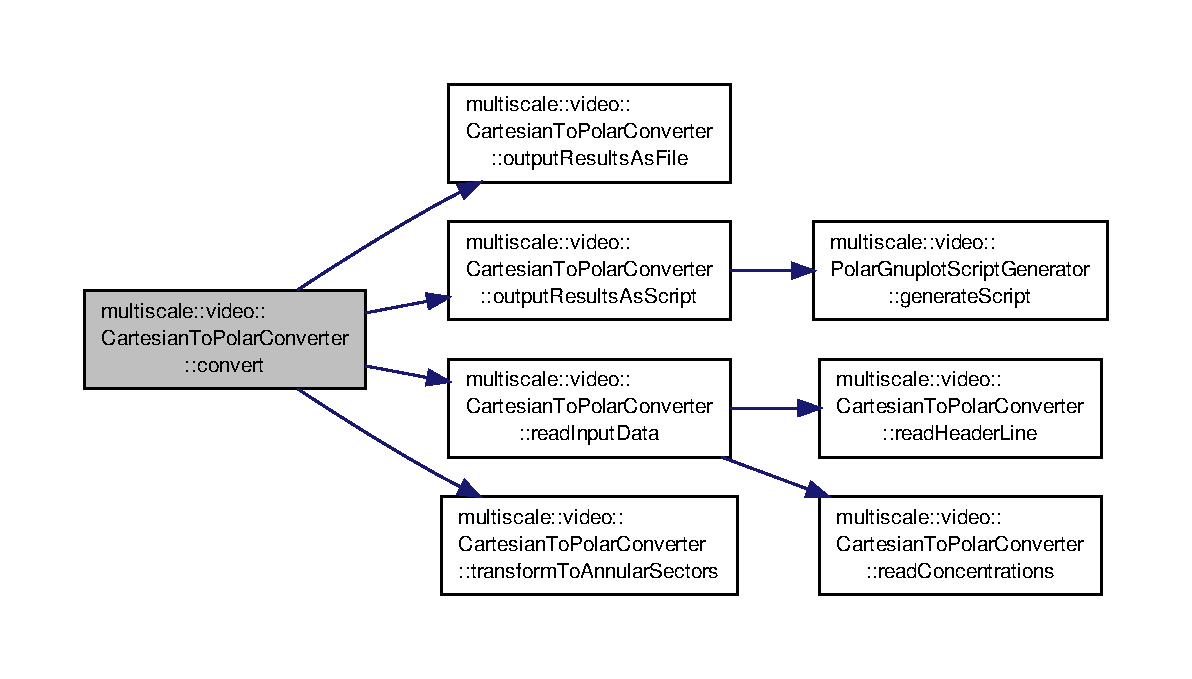
\includegraphics[width=350pt]{classmultiscale_1_1video_1_1CartesianToPolarConverter_aae3e7e842456da18741bccccdf084922_cgraph}
\end{center}
\end{figure}




\-Here is the caller graph for this function\-:
\nopagebreak
\begin{figure}[H]
\begin{center}
\leavevmode
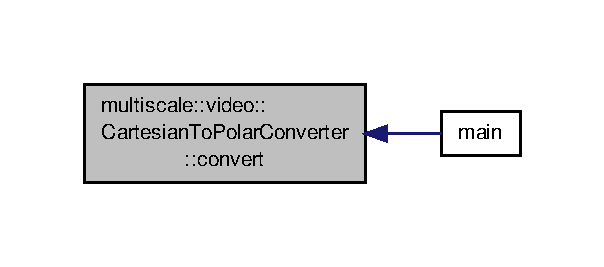
\includegraphics[width=350pt]{classmultiscale_1_1video_1_1CartesianToPolarConverter_aae3e7e842456da18741bccccdf084922_icgraph}
\end{center}
\end{figure}


\hypertarget{classmultiscale_1_1video_1_1CartesianToPolarConverter_adb3aeeb5f2994f8aa9dc03c8c8f270ad}{\index{multiscale\-::video\-::\-Cartesian\-To\-Polar\-Converter@{multiscale\-::video\-::\-Cartesian\-To\-Polar\-Converter}!output\-Results\-As\-File@{output\-Results\-As\-File}}
\index{output\-Results\-As\-File@{output\-Results\-As\-File}!multiscale::video::CartesianToPolarConverter@{multiscale\-::video\-::\-Cartesian\-To\-Polar\-Converter}}
\subsubsection[{output\-Results\-As\-File}]{\setlength{\rightskip}{0pt plus 5cm}void {\bf \-Cartesian\-To\-Polar\-Converter\-::output\-Results\-As\-File} (
\begin{DoxyParamCaption}
{}
\end{DoxyParamCaption}
)\hspace{0.3cm}{\ttfamily  \mbox{[}private\mbox{]}}}}\label{classmultiscale_1_1video_1_1CartesianToPolarConverter_adb3aeeb5f2994f8aa9dc03c8c8f270ad}


\-Output the results as a plain file. 



\-Definition at line 116 of file \-Cartesian\-To\-Polar\-Converter.\-cpp.



\-References annular\-Sectors, \-O\-U\-T\-P\-U\-T\-\_\-\-F\-I\-L\-E\-\_\-\-E\-X\-T\-E\-N\-S\-I\-O\-N, and output\-Filepath.



\-Referenced by convert().



\-Here is the caller graph for this function\-:
\nopagebreak
\begin{figure}[H]
\begin{center}
\leavevmode
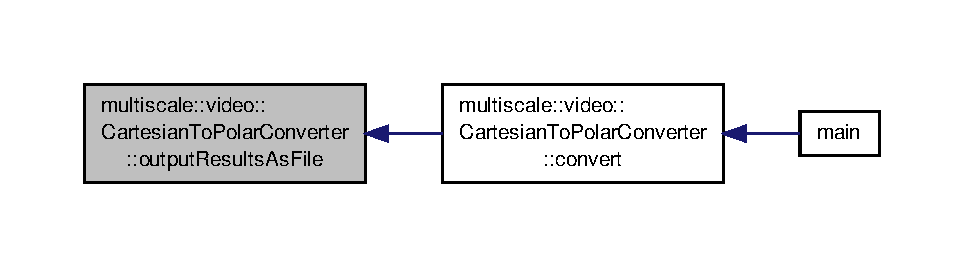
\includegraphics[width=350pt]{classmultiscale_1_1video_1_1CartesianToPolarConverter_adb3aeeb5f2994f8aa9dc03c8c8f270ad_icgraph}
\end{center}
\end{figure}


\hypertarget{classmultiscale_1_1video_1_1CartesianToPolarConverter_a680e357efb54b1193715259cb339516e}{\index{multiscale\-::video\-::\-Cartesian\-To\-Polar\-Converter@{multiscale\-::video\-::\-Cartesian\-To\-Polar\-Converter}!output\-Results\-As\-Script@{output\-Results\-As\-Script}}
\index{output\-Results\-As\-Script@{output\-Results\-As\-Script}!multiscale::video::CartesianToPolarConverter@{multiscale\-::video\-::\-Cartesian\-To\-Polar\-Converter}}
\subsubsection[{output\-Results\-As\-Script}]{\setlength{\rightskip}{0pt plus 5cm}void {\bf \-Cartesian\-To\-Polar\-Converter\-::output\-Results\-As\-Script} (
\begin{DoxyParamCaption}
{}
\end{DoxyParamCaption}
)\hspace{0.3cm}{\ttfamily  \mbox{[}private\mbox{]}}}}\label{classmultiscale_1_1video_1_1CartesianToPolarConverter_a680e357efb54b1193715259cb339516e}


\-Output the results as a gnuplot script. 



\-Definition at line 131 of file \-Cartesian\-To\-Polar\-Converter.\-cpp.



\-References annular\-Sectors, multiscale\-::video\-::\-Polar\-Gnuplot\-Script\-Generator\-::generate\-Script(), output\-Filepath, and simulation\-Time.



\-Referenced by convert().



\-Here is the call graph for this function\-:
\nopagebreak
\begin{figure}[H]
\begin{center}
\leavevmode
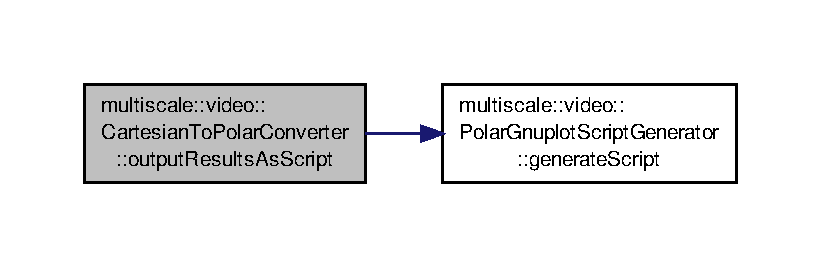
\includegraphics[width=350pt]{classmultiscale_1_1video_1_1CartesianToPolarConverter_a680e357efb54b1193715259cb339516e_cgraph}
\end{center}
\end{figure}




\-Here is the caller graph for this function\-:
\nopagebreak
\begin{figure}[H]
\begin{center}
\leavevmode
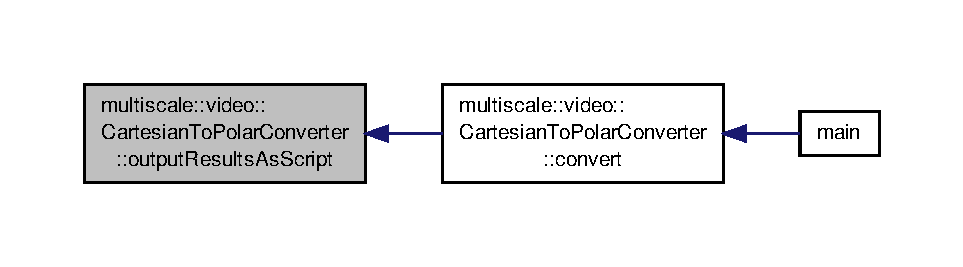
\includegraphics[width=350pt]{classmultiscale_1_1video_1_1CartesianToPolarConverter_a680e357efb54b1193715259cb339516e_icgraph}
\end{center}
\end{figure}


\hypertarget{classmultiscale_1_1video_1_1CartesianToPolarConverter_a7335cccc7e3c14203b00357ec6a2c140}{\index{multiscale\-::video\-::\-Cartesian\-To\-Polar\-Converter@{multiscale\-::video\-::\-Cartesian\-To\-Polar\-Converter}!read\-Concentrations@{read\-Concentrations}}
\index{read\-Concentrations@{read\-Concentrations}!multiscale::video::CartesianToPolarConverter@{multiscale\-::video\-::\-Cartesian\-To\-Polar\-Converter}}
\subsubsection[{read\-Concentrations}]{\setlength{\rightskip}{0pt plus 5cm}void {\bf \-Cartesian\-To\-Polar\-Converter\-::read\-Concentrations} (
\begin{DoxyParamCaption}
\item[{ifstream \&}]{fin}
\end{DoxyParamCaption}
)\hspace{0.3cm}{\ttfamily  \mbox{[}private\mbox{]}}}}\label{classmultiscale_1_1video_1_1CartesianToPolarConverter_a7335cccc7e3c14203b00357ec6a2c140}


\-Read the concentrations. 


\begin{DoxyParams}{\-Parameters}
{\em fin} & \-Input file stream \\
\hline
\end{DoxyParams}


\-Definition at line 71 of file \-Cartesian\-To\-Polar\-Converter.\-cpp.



\-References concentrations, \-E\-R\-R\-\_\-\-C\-O\-N\-C, \-M\-S\-\_\-throw, nr\-Of\-Concentric\-Circles, and nr\-Of\-Sectors.



\-Referenced by read\-Input\-Data().



\-Here is the caller graph for this function\-:
\nopagebreak
\begin{figure}[H]
\begin{center}
\leavevmode
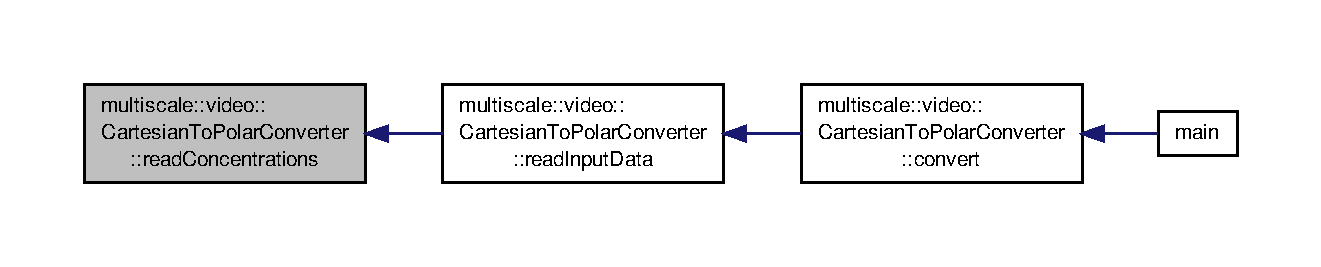
\includegraphics[width=350pt]{classmultiscale_1_1video_1_1CartesianToPolarConverter_a7335cccc7e3c14203b00357ec6a2c140_icgraph}
\end{center}
\end{figure}


\hypertarget{classmultiscale_1_1video_1_1CartesianToPolarConverter_a88d7c95fb76c9e139cb013c11a8dfae0}{\index{multiscale\-::video\-::\-Cartesian\-To\-Polar\-Converter@{multiscale\-::video\-::\-Cartesian\-To\-Polar\-Converter}!read\-Header\-Line@{read\-Header\-Line}}
\index{read\-Header\-Line@{read\-Header\-Line}!multiscale::video::CartesianToPolarConverter@{multiscale\-::video\-::\-Cartesian\-To\-Polar\-Converter}}
\subsubsection[{read\-Header\-Line}]{\setlength{\rightskip}{0pt plus 5cm}void {\bf \-Cartesian\-To\-Polar\-Converter\-::read\-Header\-Line} (
\begin{DoxyParamCaption}
\item[{ifstream \&}]{fin}
\end{DoxyParamCaption}
)\hspace{0.3cm}{\ttfamily  \mbox{[}private\mbox{]}}}}\label{classmultiscale_1_1video_1_1CartesianToPolarConverter_a88d7c95fb76c9e139cb013c11a8dfae0}


\-Read the header line. 

\-The header line contains values for number of concentric circles, number of sectors and simulation time


\begin{DoxyParams}{\-Parameters}
{\em fin} & \-Input file stream \\
\hline
\end{DoxyParams}


\-Definition at line 62 of file \-Cartesian\-To\-Polar\-Converter.\-cpp.



\-References \-E\-R\-R\-\_\-\-N\-E\-G\-\_\-\-S\-I\-M\-\_\-\-T\-I\-M\-E, \-E\-R\-R\-\_\-\-N\-O\-N\-P\-O\-S\-\_\-\-D\-I\-M\-E\-N\-S\-I\-O\-N, \-M\-S\-\_\-throw, nr\-Of\-Concentric\-Circles, nr\-Of\-Sectors, and simulation\-Time.



\-Referenced by read\-Input\-Data().



\-Here is the caller graph for this function\-:
\nopagebreak
\begin{figure}[H]
\begin{center}
\leavevmode
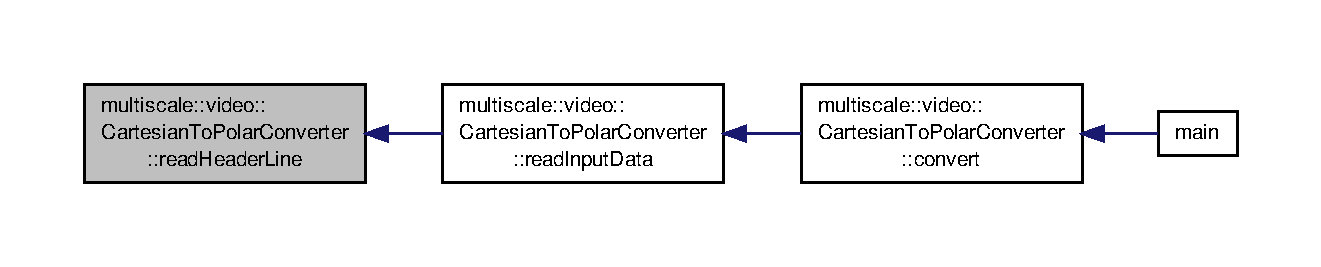
\includegraphics[width=350pt]{classmultiscale_1_1video_1_1CartesianToPolarConverter_a88d7c95fb76c9e139cb013c11a8dfae0_icgraph}
\end{center}
\end{figure}


\hypertarget{classmultiscale_1_1video_1_1CartesianToPolarConverter_a37891007ade23e05047d33d0c9cb3e13}{\index{multiscale\-::video\-::\-Cartesian\-To\-Polar\-Converter@{multiscale\-::video\-::\-Cartesian\-To\-Polar\-Converter}!read\-Input\-Data@{read\-Input\-Data}}
\index{read\-Input\-Data@{read\-Input\-Data}!multiscale::video::CartesianToPolarConverter@{multiscale\-::video\-::\-Cartesian\-To\-Polar\-Converter}}
\subsubsection[{read\-Input\-Data}]{\setlength{\rightskip}{0pt plus 5cm}void {\bf \-Cartesian\-To\-Polar\-Converter\-::read\-Input\-Data} (
\begin{DoxyParamCaption}
{}
\end{DoxyParamCaption}
)\hspace{0.3cm}{\ttfamily  \mbox{[}private\mbox{]}}}}\label{classmultiscale_1_1video_1_1CartesianToPolarConverter_a37891007ade23e05047d33d0c9cb3e13}


\-Read the input data. 



\-Definition at line 38 of file \-Cartesian\-To\-Polar\-Converter.\-cpp.



\-References \-E\-R\-R\-\_\-\-I\-N\-\_\-\-E\-X\-T\-R\-A\-\_\-\-D\-A\-T\-A, \-E\-R\-R\-\_\-\-I\-N\-P\-U\-T\-\_\-\-O\-P\-E\-N, input\-Filepath, \-M\-S\-\_\-throw, read\-Concentrations(), and read\-Header\-Line().



\-Referenced by convert().



\-Here is the call graph for this function\-:
\nopagebreak
\begin{figure}[H]
\begin{center}
\leavevmode
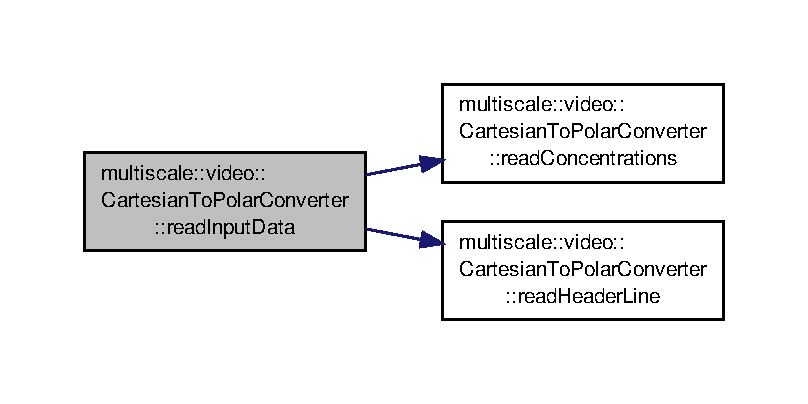
\includegraphics[width=350pt]{classmultiscale_1_1video_1_1CartesianToPolarConverter_a37891007ade23e05047d33d0c9cb3e13_cgraph}
\end{center}
\end{figure}




\-Here is the caller graph for this function\-:
\nopagebreak
\begin{figure}[H]
\begin{center}
\leavevmode
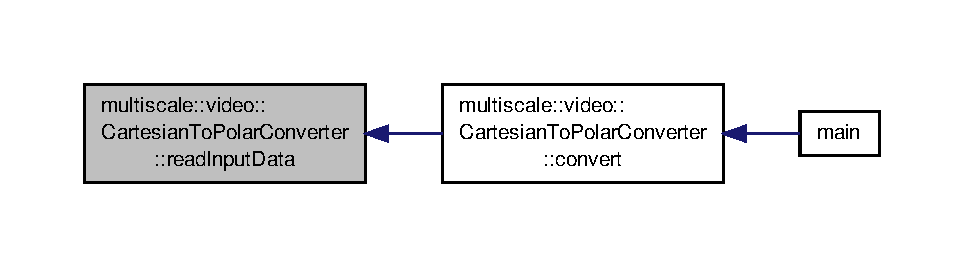
\includegraphics[width=350pt]{classmultiscale_1_1video_1_1CartesianToPolarConverter_a37891007ade23e05047d33d0c9cb3e13_icgraph}
\end{center}
\end{figure}


\hypertarget{classmultiscale_1_1video_1_1CartesianToPolarConverter_a0c3f499725a058d2a3251209d8c16178}{\index{multiscale\-::video\-::\-Cartesian\-To\-Polar\-Converter@{multiscale\-::video\-::\-Cartesian\-To\-Polar\-Converter}!transform\-To\-Annular\-Sectors@{transform\-To\-Annular\-Sectors}}
\index{transform\-To\-Annular\-Sectors@{transform\-To\-Annular\-Sectors}!multiscale::video::CartesianToPolarConverter@{multiscale\-::video\-::\-Cartesian\-To\-Polar\-Converter}}
\subsubsection[{transform\-To\-Annular\-Sectors}]{\setlength{\rightskip}{0pt plus 5cm}void {\bf \-Cartesian\-To\-Polar\-Converter\-::transform\-To\-Annular\-Sectors} (
\begin{DoxyParamCaption}
{}
\end{DoxyParamCaption}
)\hspace{0.3cm}{\ttfamily  \mbox{[}private\mbox{]}}}}\label{classmultiscale_1_1video_1_1CartesianToPolarConverter_a0c3f499725a058d2a3251209d8c16178}


\-Convert the concentrations to annular sectors. 



\-Definition at line 91 of file \-Cartesian\-To\-Polar\-Converter.\-cpp.



\-References annular\-Sectors, concentrations, nr\-Of\-Concentric\-Circles, nr\-Of\-Sectors, \-R\-A\-D\-I\-U\-S\-\_\-\-M\-A\-X, and \-R\-A\-D\-I\-U\-S\-\_\-\-M\-I\-N.



\-Referenced by convert().



\-Here is the caller graph for this function\-:
\nopagebreak
\begin{figure}[H]
\begin{center}
\leavevmode
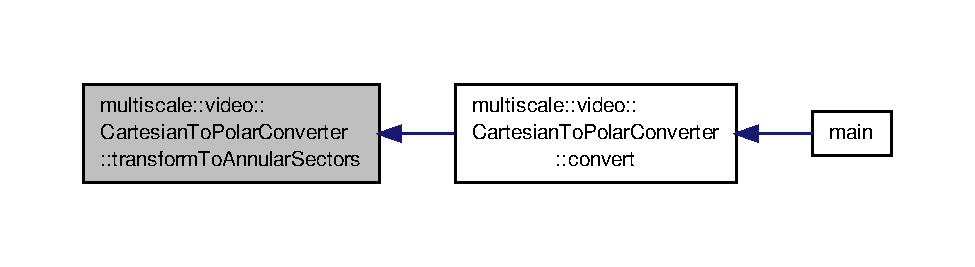
\includegraphics[width=350pt]{classmultiscale_1_1video_1_1CartesianToPolarConverter_a0c3f499725a058d2a3251209d8c16178_icgraph}
\end{center}
\end{figure}




\subsection{\-Member \-Data \-Documentation}
\hypertarget{classmultiscale_1_1video_1_1CartesianToPolarConverter_a3f8004ac5f8bae93c7a5e09bc37ba0ac}{\index{multiscale\-::video\-::\-Cartesian\-To\-Polar\-Converter@{multiscale\-::video\-::\-Cartesian\-To\-Polar\-Converter}!annular\-Sectors@{annular\-Sectors}}
\index{annular\-Sectors@{annular\-Sectors}!multiscale::video::CartesianToPolarConverter@{multiscale\-::video\-::\-Cartesian\-To\-Polar\-Converter}}
\subsubsection[{annular\-Sectors}]{\setlength{\rightskip}{0pt plus 5cm}vector$<${\bf \-Annular\-Sector}$>$ {\bf multiscale\-::video\-::\-Cartesian\-To\-Polar\-Converter\-::annular\-Sectors}\hspace{0.3cm}{\ttfamily  \mbox{[}private\mbox{]}}}}\label{classmultiscale_1_1video_1_1CartesianToPolarConverter_a3f8004ac5f8bae93c7a5e09bc37ba0ac}
\-Resulting annular sectors 

\-Definition at line 21 of file \-Cartesian\-To\-Polar\-Converter.\-hpp.



\-Referenced by output\-Results\-As\-File(), output\-Results\-As\-Script(), and transform\-To\-Annular\-Sectors().

\hypertarget{classmultiscale_1_1video_1_1CartesianToPolarConverter_a7356e201623f518132d75b7bc48407d3}{\index{multiscale\-::video\-::\-Cartesian\-To\-Polar\-Converter@{multiscale\-::video\-::\-Cartesian\-To\-Polar\-Converter}!concentrations@{concentrations}}
\index{concentrations@{concentrations}!multiscale::video::CartesianToPolarConverter@{multiscale\-::video\-::\-Cartesian\-To\-Polar\-Converter}}
\subsubsection[{concentrations}]{\setlength{\rightskip}{0pt plus 5cm}vector$<$double$>$ {\bf multiscale\-::video\-::\-Cartesian\-To\-Polar\-Converter\-::concentrations}\hspace{0.3cm}{\ttfamily  \mbox{[}private\mbox{]}}}}\label{classmultiscale_1_1video_1_1CartesianToPolarConverter_a7356e201623f518132d75b7bc48407d3}
\-Concentrations received as input 

\-Definition at line 22 of file \-Cartesian\-To\-Polar\-Converter.\-hpp.



\-Referenced by read\-Concentrations(), and transform\-To\-Annular\-Sectors().

\hypertarget{classmultiscale_1_1video_1_1CartesianToPolarConverter_a2657e7972c2d3f7cc4c0011ccd8423e4}{\index{multiscale\-::video\-::\-Cartesian\-To\-Polar\-Converter@{multiscale\-::video\-::\-Cartesian\-To\-Polar\-Converter}!\-E\-R\-R\-\_\-\-C\-O\-N\-C@{\-E\-R\-R\-\_\-\-C\-O\-N\-C}}
\index{\-E\-R\-R\-\_\-\-C\-O\-N\-C@{\-E\-R\-R\-\_\-\-C\-O\-N\-C}!multiscale::video::CartesianToPolarConverter@{multiscale\-::video\-::\-Cartesian\-To\-Polar\-Converter}}
\subsubsection[{\-E\-R\-R\-\_\-\-C\-O\-N\-C}]{\setlength{\rightskip}{0pt plus 5cm}const string {\bf \-Cartesian\-To\-Polar\-Converter\-::\-E\-R\-R\-\_\-\-C\-O\-N\-C} = \char`\"{}\-All {\bf concentrations} have to be between 0 and 1.\char`\"{}\hspace{0.3cm}{\ttfamily  \mbox{[}static, private\mbox{]}}}}\label{classmultiscale_1_1video_1_1CartesianToPolarConverter_a2657e7972c2d3f7cc4c0011ccd8423e4}


\-Definition at line 74 of file \-Cartesian\-To\-Polar\-Converter.\-hpp.



\-Referenced by read\-Concentrations().

\hypertarget{classmultiscale_1_1video_1_1CartesianToPolarConverter_a27c4664c63c53cc5351bbb3233bdfce1}{\index{multiscale\-::video\-::\-Cartesian\-To\-Polar\-Converter@{multiscale\-::video\-::\-Cartesian\-To\-Polar\-Converter}!\-E\-R\-R\-\_\-\-I\-N\-\_\-\-E\-X\-T\-R\-A\-\_\-\-D\-A\-T\-A@{\-E\-R\-R\-\_\-\-I\-N\-\_\-\-E\-X\-T\-R\-A\-\_\-\-D\-A\-T\-A}}
\index{\-E\-R\-R\-\_\-\-I\-N\-\_\-\-E\-X\-T\-R\-A\-\_\-\-D\-A\-T\-A@{\-E\-R\-R\-\_\-\-I\-N\-\_\-\-E\-X\-T\-R\-A\-\_\-\-D\-A\-T\-A}!multiscale::video::CartesianToPolarConverter@{multiscale\-::video\-::\-Cartesian\-To\-Polar\-Converter}}
\subsubsection[{\-E\-R\-R\-\_\-\-I\-N\-\_\-\-E\-X\-T\-R\-A\-\_\-\-D\-A\-T\-A}]{\setlength{\rightskip}{0pt plus 5cm}const string {\bf \-Cartesian\-To\-Polar\-Converter\-::\-E\-R\-R\-\_\-\-I\-N\-\_\-\-E\-X\-T\-R\-A\-\_\-\-D\-A\-T\-A} = \char`\"{}\-The input file contains more data than required.\char`\"{}\hspace{0.3cm}{\ttfamily  \mbox{[}static, private\mbox{]}}}}\label{classmultiscale_1_1video_1_1CartesianToPolarConverter_a27c4664c63c53cc5351bbb3233bdfce1}


\-Definition at line 78 of file \-Cartesian\-To\-Polar\-Converter.\-hpp.



\-Referenced by read\-Input\-Data().

\hypertarget{classmultiscale_1_1video_1_1CartesianToPolarConverter_a298f7aba7ec17e486484fa2e52ebc109}{\index{multiscale\-::video\-::\-Cartesian\-To\-Polar\-Converter@{multiscale\-::video\-::\-Cartesian\-To\-Polar\-Converter}!\-E\-R\-R\-\_\-\-I\-N\-P\-U\-T\-\_\-\-O\-P\-E\-N@{\-E\-R\-R\-\_\-\-I\-N\-P\-U\-T\-\_\-\-O\-P\-E\-N}}
\index{\-E\-R\-R\-\_\-\-I\-N\-P\-U\-T\-\_\-\-O\-P\-E\-N@{\-E\-R\-R\-\_\-\-I\-N\-P\-U\-T\-\_\-\-O\-P\-E\-N}!multiscale::video::CartesianToPolarConverter@{multiscale\-::video\-::\-Cartesian\-To\-Polar\-Converter}}
\subsubsection[{\-E\-R\-R\-\_\-\-I\-N\-P\-U\-T\-\_\-\-O\-P\-E\-N}]{\setlength{\rightskip}{0pt plus 5cm}const string {\bf \-Cartesian\-To\-Polar\-Converter\-::\-E\-R\-R\-\_\-\-I\-N\-P\-U\-T\-\_\-\-O\-P\-E\-N} = \char`\"{}\-The input file could not be opened\char`\"{}\hspace{0.3cm}{\ttfamily  \mbox{[}static, private\mbox{]}}}}\label{classmultiscale_1_1video_1_1CartesianToPolarConverter_a298f7aba7ec17e486484fa2e52ebc109}


\-Definition at line 77 of file \-Cartesian\-To\-Polar\-Converter.\-hpp.



\-Referenced by read\-Input\-Data().

\hypertarget{classmultiscale_1_1video_1_1CartesianToPolarConverter_a0a3ab913d167193883dc96aed6cc8290}{\index{multiscale\-::video\-::\-Cartesian\-To\-Polar\-Converter@{multiscale\-::video\-::\-Cartesian\-To\-Polar\-Converter}!\-E\-R\-R\-\_\-\-N\-E\-G\-\_\-\-S\-I\-M\-\_\-\-T\-I\-M\-E@{\-E\-R\-R\-\_\-\-N\-E\-G\-\_\-\-S\-I\-M\-\_\-\-T\-I\-M\-E}}
\index{\-E\-R\-R\-\_\-\-N\-E\-G\-\_\-\-S\-I\-M\-\_\-\-T\-I\-M\-E@{\-E\-R\-R\-\_\-\-N\-E\-G\-\_\-\-S\-I\-M\-\_\-\-T\-I\-M\-E}!multiscale::video::CartesianToPolarConverter@{multiscale\-::video\-::\-Cartesian\-To\-Polar\-Converter}}
\subsubsection[{\-E\-R\-R\-\_\-\-N\-E\-G\-\_\-\-S\-I\-M\-\_\-\-T\-I\-M\-E}]{\setlength{\rightskip}{0pt plus 5cm}const string {\bf \-Cartesian\-To\-Polar\-Converter\-::\-E\-R\-R\-\_\-\-N\-E\-G\-\_\-\-S\-I\-M\-\_\-\-T\-I\-M\-E} = \char`\"{}\-The simulation time must be non-\/negative.\char`\"{}\hspace{0.3cm}{\ttfamily  \mbox{[}static, private\mbox{]}}}}\label{classmultiscale_1_1video_1_1CartesianToPolarConverter_a0a3ab913d167193883dc96aed6cc8290}


\-Definition at line 76 of file \-Cartesian\-To\-Polar\-Converter.\-hpp.



\-Referenced by read\-Header\-Line().

\hypertarget{classmultiscale_1_1video_1_1CartesianToPolarConverter_ab3a2114f4dd2615abba3305609f1b616}{\index{multiscale\-::video\-::\-Cartesian\-To\-Polar\-Converter@{multiscale\-::video\-::\-Cartesian\-To\-Polar\-Converter}!\-E\-R\-R\-\_\-\-N\-O\-N\-P\-O\-S\-\_\-\-D\-I\-M\-E\-N\-S\-I\-O\-N@{\-E\-R\-R\-\_\-\-N\-O\-N\-P\-O\-S\-\_\-\-D\-I\-M\-E\-N\-S\-I\-O\-N}}
\index{\-E\-R\-R\-\_\-\-N\-O\-N\-P\-O\-S\-\_\-\-D\-I\-M\-E\-N\-S\-I\-O\-N@{\-E\-R\-R\-\_\-\-N\-O\-N\-P\-O\-S\-\_\-\-D\-I\-M\-E\-N\-S\-I\-O\-N}!multiscale::video::CartesianToPolarConverter@{multiscale\-::video\-::\-Cartesian\-To\-Polar\-Converter}}
\subsubsection[{\-E\-R\-R\-\_\-\-N\-O\-N\-P\-O\-S\-\_\-\-D\-I\-M\-E\-N\-S\-I\-O\-N}]{\setlength{\rightskip}{0pt plus 5cm}const string {\bf \-Cartesian\-To\-Polar\-Converter\-::\-E\-R\-R\-\_\-\-N\-O\-N\-P\-O\-S\-\_\-\-D\-I\-M\-E\-N\-S\-I\-O\-N} = \char`\"{}\-The dimensions \-N and \-M must be positive.\char`\"{}\hspace{0.3cm}{\ttfamily  \mbox{[}static, private\mbox{]}}}}\label{classmultiscale_1_1video_1_1CartesianToPolarConverter_ab3a2114f4dd2615abba3305609f1b616}


\-Definition at line 75 of file \-Cartesian\-To\-Polar\-Converter.\-hpp.



\-Referenced by read\-Header\-Line().

\hypertarget{classmultiscale_1_1video_1_1CartesianToPolarConverter_aa15eca9e8d3da0eb8ff1b6583e392f05}{\index{multiscale\-::video\-::\-Cartesian\-To\-Polar\-Converter@{multiscale\-::video\-::\-Cartesian\-To\-Polar\-Converter}!input\-Filepath@{input\-Filepath}}
\index{input\-Filepath@{input\-Filepath}!multiscale::video::CartesianToPolarConverter@{multiscale\-::video\-::\-Cartesian\-To\-Polar\-Converter}}
\subsubsection[{input\-Filepath}]{\setlength{\rightskip}{0pt plus 5cm}string {\bf multiscale\-::video\-::\-Cartesian\-To\-Polar\-Converter\-::input\-Filepath}\hspace{0.3cm}{\ttfamily  \mbox{[}private\mbox{]}}}}\label{classmultiscale_1_1video_1_1CartesianToPolarConverter_aa15eca9e8d3da0eb8ff1b6583e392f05}
\-Path to the input file 

\-Definition at line 28 of file \-Cartesian\-To\-Polar\-Converter.\-hpp.



\-Referenced by read\-Input\-Data().

\hypertarget{classmultiscale_1_1video_1_1CartesianToPolarConverter_ab7c8564deaa38c57a251ba9592903238}{\index{multiscale\-::video\-::\-Cartesian\-To\-Polar\-Converter@{multiscale\-::video\-::\-Cartesian\-To\-Polar\-Converter}!nr\-Of\-Concentric\-Circles@{nr\-Of\-Concentric\-Circles}}
\index{nr\-Of\-Concentric\-Circles@{nr\-Of\-Concentric\-Circles}!multiscale::video::CartesianToPolarConverter@{multiscale\-::video\-::\-Cartesian\-To\-Polar\-Converter}}
\subsubsection[{nr\-Of\-Concentric\-Circles}]{\setlength{\rightskip}{0pt plus 5cm}unsigned long {\bf multiscale\-::video\-::\-Cartesian\-To\-Polar\-Converter\-::nr\-Of\-Concentric\-Circles}\hspace{0.3cm}{\ttfamily  \mbox{[}private\mbox{]}}}}\label{classmultiscale_1_1video_1_1CartesianToPolarConverter_ab7c8564deaa38c57a251ba9592903238}
\-Number of concentric circles 

\-Definition at line 24 of file \-Cartesian\-To\-Polar\-Converter.\-hpp.



\-Referenced by \-Cartesian\-To\-Polar\-Converter(), read\-Concentrations(), read\-Header\-Line(), and transform\-To\-Annular\-Sectors().

\hypertarget{classmultiscale_1_1video_1_1CartesianToPolarConverter_a62a2f5abe655f440e7c41fe834f828d0}{\index{multiscale\-::video\-::\-Cartesian\-To\-Polar\-Converter@{multiscale\-::video\-::\-Cartesian\-To\-Polar\-Converter}!nr\-Of\-Sectors@{nr\-Of\-Sectors}}
\index{nr\-Of\-Sectors@{nr\-Of\-Sectors}!multiscale::video::CartesianToPolarConverter@{multiscale\-::video\-::\-Cartesian\-To\-Polar\-Converter}}
\subsubsection[{nr\-Of\-Sectors}]{\setlength{\rightskip}{0pt plus 5cm}unsigned long {\bf multiscale\-::video\-::\-Cartesian\-To\-Polar\-Converter\-::nr\-Of\-Sectors}\hspace{0.3cm}{\ttfamily  \mbox{[}private\mbox{]}}}}\label{classmultiscale_1_1video_1_1CartesianToPolarConverter_a62a2f5abe655f440e7c41fe834f828d0}
\-Number of sectors 

\-Definition at line 25 of file \-Cartesian\-To\-Polar\-Converter.\-hpp.



\-Referenced by \-Cartesian\-To\-Polar\-Converter(), read\-Concentrations(), read\-Header\-Line(), and transform\-To\-Annular\-Sectors().

\hypertarget{classmultiscale_1_1video_1_1CartesianToPolarConverter_a3dcad19e1da427627d783a3053174372}{\index{multiscale\-::video\-::\-Cartesian\-To\-Polar\-Converter@{multiscale\-::video\-::\-Cartesian\-To\-Polar\-Converter}!\-O\-U\-T\-P\-U\-T\-\_\-\-F\-I\-L\-E\-\_\-\-E\-X\-T\-E\-N\-S\-I\-O\-N@{\-O\-U\-T\-P\-U\-T\-\_\-\-F\-I\-L\-E\-\_\-\-E\-X\-T\-E\-N\-S\-I\-O\-N}}
\index{\-O\-U\-T\-P\-U\-T\-\_\-\-F\-I\-L\-E\-\_\-\-E\-X\-T\-E\-N\-S\-I\-O\-N@{\-O\-U\-T\-P\-U\-T\-\_\-\-F\-I\-L\-E\-\_\-\-E\-X\-T\-E\-N\-S\-I\-O\-N}!multiscale::video::CartesianToPolarConverter@{multiscale\-::video\-::\-Cartesian\-To\-Polar\-Converter}}
\subsubsection[{\-O\-U\-T\-P\-U\-T\-\_\-\-F\-I\-L\-E\-\_\-\-E\-X\-T\-E\-N\-S\-I\-O\-N}]{\setlength{\rightskip}{0pt plus 5cm}const string {\bf \-Cartesian\-To\-Polar\-Converter\-::\-O\-U\-T\-P\-U\-T\-\_\-\-F\-I\-L\-E\-\_\-\-E\-X\-T\-E\-N\-S\-I\-O\-N} = \char`\"{}.out\char`\"{}\hspace{0.3cm}{\ttfamily  \mbox{[}static, private\mbox{]}}}}\label{classmultiscale_1_1video_1_1CartesianToPolarConverter_a3dcad19e1da427627d783a3053174372}


\-Definition at line 80 of file \-Cartesian\-To\-Polar\-Converter.\-hpp.



\-Referenced by output\-Results\-As\-File().

\hypertarget{classmultiscale_1_1video_1_1CartesianToPolarConverter_a024d95ab3b9de6ed6fd1d951c5575e65}{\index{multiscale\-::video\-::\-Cartesian\-To\-Polar\-Converter@{multiscale\-::video\-::\-Cartesian\-To\-Polar\-Converter}!output\-Filepath@{output\-Filepath}}
\index{output\-Filepath@{output\-Filepath}!multiscale::video::CartesianToPolarConverter@{multiscale\-::video\-::\-Cartesian\-To\-Polar\-Converter}}
\subsubsection[{output\-Filepath}]{\setlength{\rightskip}{0pt plus 5cm}string {\bf multiscale\-::video\-::\-Cartesian\-To\-Polar\-Converter\-::output\-Filepath}\hspace{0.3cm}{\ttfamily  \mbox{[}private\mbox{]}}}}\label{classmultiscale_1_1video_1_1CartesianToPolarConverter_a024d95ab3b9de6ed6fd1d951c5575e65}
\-Path to the output file 

\-Definition at line 29 of file \-Cartesian\-To\-Polar\-Converter.\-hpp.



\-Referenced by output\-Results\-As\-File(), and output\-Results\-As\-Script().

\hypertarget{classmultiscale_1_1video_1_1CartesianToPolarConverter_a79bb03defe0d68884ce5d4f1b0a7d60c}{\index{multiscale\-::video\-::\-Cartesian\-To\-Polar\-Converter@{multiscale\-::video\-::\-Cartesian\-To\-Polar\-Converter}!\-R\-A\-D\-I\-U\-S\-\_\-\-M\-A\-X@{\-R\-A\-D\-I\-U\-S\-\_\-\-M\-A\-X}}
\index{\-R\-A\-D\-I\-U\-S\-\_\-\-M\-A\-X@{\-R\-A\-D\-I\-U\-S\-\_\-\-M\-A\-X}!multiscale::video::CartesianToPolarConverter@{multiscale\-::video\-::\-Cartesian\-To\-Polar\-Converter}}
\subsubsection[{\-R\-A\-D\-I\-U\-S\-\_\-\-M\-A\-X}]{\setlength{\rightskip}{0pt plus 5cm}const double {\bf \-Cartesian\-To\-Polar\-Converter\-::\-R\-A\-D\-I\-U\-S\-\_\-\-M\-A\-X} = 0.\-3\hspace{0.3cm}{\ttfamily  \mbox{[}static, private\mbox{]}}}}\label{classmultiscale_1_1video_1_1CartesianToPolarConverter_a79bb03defe0d68884ce5d4f1b0a7d60c}


\-Definition at line 83 of file \-Cartesian\-To\-Polar\-Converter.\-hpp.



\-Referenced by transform\-To\-Annular\-Sectors().

\hypertarget{classmultiscale_1_1video_1_1CartesianToPolarConverter_a59c18c22603ad65bf26533dd2aafd04e}{\index{multiscale\-::video\-::\-Cartesian\-To\-Polar\-Converter@{multiscale\-::video\-::\-Cartesian\-To\-Polar\-Converter}!\-R\-A\-D\-I\-U\-S\-\_\-\-M\-I\-N@{\-R\-A\-D\-I\-U\-S\-\_\-\-M\-I\-N}}
\index{\-R\-A\-D\-I\-U\-S\-\_\-\-M\-I\-N@{\-R\-A\-D\-I\-U\-S\-\_\-\-M\-I\-N}!multiscale::video::CartesianToPolarConverter@{multiscale\-::video\-::\-Cartesian\-To\-Polar\-Converter}}
\subsubsection[{\-R\-A\-D\-I\-U\-S\-\_\-\-M\-I\-N}]{\setlength{\rightskip}{0pt plus 5cm}const double {\bf \-Cartesian\-To\-Polar\-Converter\-::\-R\-A\-D\-I\-U\-S\-\_\-\-M\-I\-N} = 0.\-001\hspace{0.3cm}{\ttfamily  \mbox{[}static, private\mbox{]}}}}\label{classmultiscale_1_1video_1_1CartesianToPolarConverter_a59c18c22603ad65bf26533dd2aafd04e}


\-Definition at line 82 of file \-Cartesian\-To\-Polar\-Converter.\-hpp.



\-Referenced by transform\-To\-Annular\-Sectors().

\hypertarget{classmultiscale_1_1video_1_1CartesianToPolarConverter_a78003dc9053d89f56c03408f7f8fedda}{\index{multiscale\-::video\-::\-Cartesian\-To\-Polar\-Converter@{multiscale\-::video\-::\-Cartesian\-To\-Polar\-Converter}!simulation\-Time@{simulation\-Time}}
\index{simulation\-Time@{simulation\-Time}!multiscale::video::CartesianToPolarConverter@{multiscale\-::video\-::\-Cartesian\-To\-Polar\-Converter}}
\subsubsection[{simulation\-Time}]{\setlength{\rightskip}{0pt plus 5cm}double {\bf multiscale\-::video\-::\-Cartesian\-To\-Polar\-Converter\-::simulation\-Time}\hspace{0.3cm}{\ttfamily  \mbox{[}private\mbox{]}}}}\label{classmultiscale_1_1video_1_1CartesianToPolarConverter_a78003dc9053d89f56c03408f7f8fedda}
\-Simulation time corresponding to the input data 

\-Definition at line 26 of file \-Cartesian\-To\-Polar\-Converter.\-hpp.



\-Referenced by \-Cartesian\-To\-Polar\-Converter(), output\-Results\-As\-Script(), and read\-Header\-Line().



\-The documentation for this class was generated from the following files\-:\begin{DoxyCompactItemize}
\item 
/home/ovidiu/\-Repositories/git/multiscale/\-Multiscale/modules/video/circular/include/multiscale/video/circular/\hyperlink{CartesianToPolarConverter_8hpp}{\-Cartesian\-To\-Polar\-Converter.\-hpp}\item 
/home/ovidiu/\-Repositories/git/multiscale/\-Multiscale/modules/video/circular/src/\hyperlink{CartesianToPolarConverter_8cpp}{\-Cartesian\-To\-Polar\-Converter.\-cpp}\end{DoxyCompactItemize}

\hypertarget{classmultiscale_1_1LexicographicNumberIterator}{\section{multiscale\-:\-:\-Lexicographic\-Number\-Iterator \-Class \-Reference}
\label{classmultiscale_1_1LexicographicNumberIterator}\index{multiscale\-::\-Lexicographic\-Number\-Iterator@{multiscale\-::\-Lexicographic\-Number\-Iterator}}
}


\-Iterator class starting at 1 and ending at the provided upper bound considering that each number is followed by an \char`\"{}\-\_\-\char`\"{}.  




{\ttfamily \#include $<$\-Lexicographic\-Number\-Iterator.\-hpp$>$}



\-Inheritance diagram for multiscale\-:\-:\-Lexicographic\-Number\-Iterator\-:
\nopagebreak
\begin{figure}[H]
\begin{center}
\leavevmode
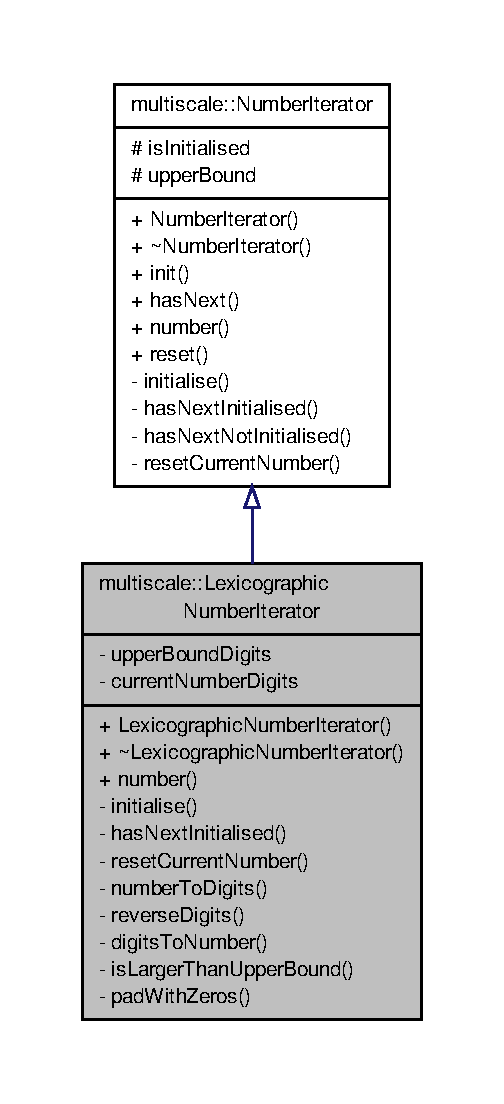
\includegraphics[width=272pt]{classmultiscale_1_1LexicographicNumberIterator__inherit__graph}
\end{center}
\end{figure}


\-Collaboration diagram for multiscale\-:\-:\-Lexicographic\-Number\-Iterator\-:
\nopagebreak
\begin{figure}[H]
\begin{center}
\leavevmode
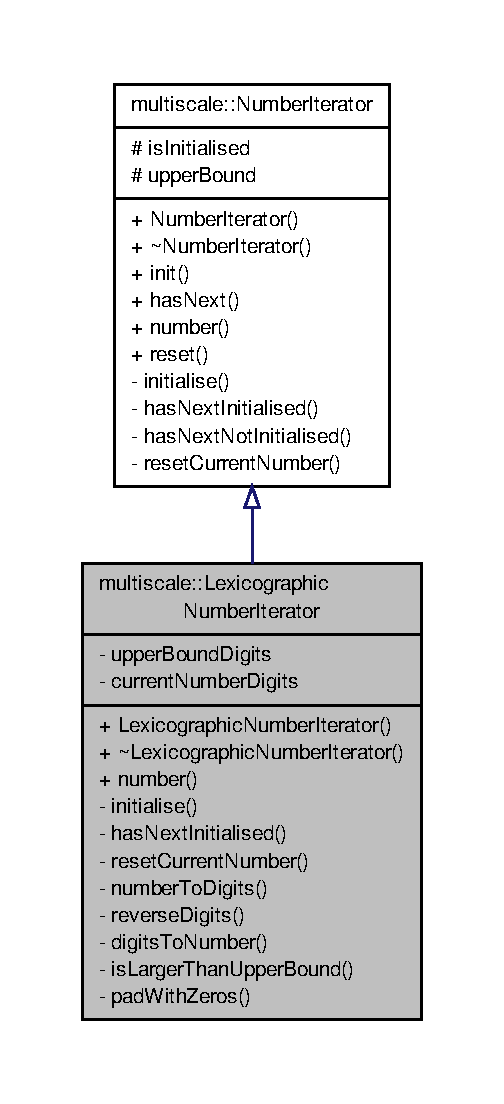
\includegraphics[height=550pt]{classmultiscale_1_1LexicographicNumberIterator__coll__graph}
\end{center}
\end{figure}
\subsection*{\-Public \-Member \-Functions}
\begin{DoxyCompactItemize}
\item 
\hyperlink{classmultiscale_1_1LexicographicNumberIterator_a02a95a6f7876b84909e08555730ff08a}{\-Lexicographic\-Number\-Iterator} (unsigned int \hyperlink{classmultiscale_1_1NumberIterator_a56a5558958778bbde64e249d67cba886}{upper\-Bound})
\item 
\hyperlink{classmultiscale_1_1LexicographicNumberIterator_affe04d9733b7d0984a5ab3957cb0096a}{$\sim$\-Lexicographic\-Number\-Iterator} ()
\item 
unsigned int \hyperlink{classmultiscale_1_1LexicographicNumberIterator_a282d970d0d1a33d2736bbdf104c18336}{number} ()
\begin{DoxyCompactList}\small\item\em \-Get the number pointed by the iterator. \end{DoxyCompactList}\end{DoxyCompactItemize}
\subsection*{\-Private \-Member \-Functions}
\begin{DoxyCompactItemize}
\item 
void \hyperlink{classmultiscale_1_1LexicographicNumberIterator_a943745c4723ed8c3c18df9f92bf94d2c}{initialise} ()
\begin{DoxyCompactList}\small\item\em \-Initialise the vectors of digits. \end{DoxyCompactList}\item 
bool \hyperlink{classmultiscale_1_1LexicographicNumberIterator_ac2754a1a57005183e2c9040719c97448}{has\-Next\-Initialised} ()
\begin{DoxyCompactList}\small\item\em \-Check if there is a next number when in initialised state. \end{DoxyCompactList}\item 
void \hyperlink{classmultiscale_1_1LexicographicNumberIterator_a18311f68a49156a415c817a947abcd7d}{reset\-Current\-Number} ()
\begin{DoxyCompactList}\small\item\em \-Reset the digits of the current number to the initial value. \end{DoxyCompactList}\item 
void \hyperlink{classmultiscale_1_1LexicographicNumberIterator_a700e18593ba0cc764d4e517993bd3fdc}{number\-To\-Digits} (unsigned int \hyperlink{classmultiscale_1_1LexicographicNumberIterator_a282d970d0d1a33d2736bbdf104c18336}{number}, vector$<$ unsigned char $>$ \&digits)
\begin{DoxyCompactList}\small\item\em \-Convert the number to a vector of digits. \end{DoxyCompactList}\item 
void \hyperlink{classmultiscale_1_1LexicographicNumberIterator_a4c0a17e03a12256584d9ed3ae19a78c9}{reverse\-Digits} (vector$<$ unsigned char $>$ \&digits)
\begin{DoxyCompactList}\small\item\em \-Reverse the order of the digits. \end{DoxyCompactList}\item 
unsigned int \hyperlink{classmultiscale_1_1LexicographicNumberIterator_a9bcb610b3b63b02ceed7d556960e57c3}{digits\-To\-Number} (vector$<$ unsigned char $>$ \&digits)
\begin{DoxyCompactList}\small\item\em \-Convert the vector of digits to the number they represent. \end{DoxyCompactList}\item 
bool \hyperlink{classmultiscale_1_1LexicographicNumberIterator_a8fad6e84a483cee3bd52c926de73d15f}{is\-Larger\-Than\-Upper\-Bound} (unsigned char last\-Digit)
\begin{DoxyCompactList}\small\item\em \-Check if the current number with the provided last digit is greater than the upper bound. \end{DoxyCompactList}\item 
void \hyperlink{classmultiscale_1_1LexicographicNumberIterator_a063dc7e6097724e96ed36bab4d20871b}{pad\-With\-Zeros} ()
\begin{DoxyCompactList}\small\item\em \-Pad the current number with zeros. \end{DoxyCompactList}\end{DoxyCompactItemize}
\subsection*{\-Private \-Attributes}
\begin{DoxyCompactItemize}
\item 
vector$<$ unsigned char $>$ \hyperlink{classmultiscale_1_1LexicographicNumberIterator_a909a054ae4d3e79e5daa3059a94000d0}{upper\-Bound\-Digits}
\item 
vector$<$ unsigned char $>$ \hyperlink{classmultiscale_1_1LexicographicNumberIterator_af42ebeea695a31c2da714332c520ae79}{current\-Number\-Digits}
\end{DoxyCompactItemize}


\subsection{\-Detailed \-Description}
\-Iterator class starting at 1 and ending at the provided upper bound considering that each number is followed by an \char`\"{}\-\_\-\char`\"{}. 

\-Definition at line 14 of file \-Lexicographic\-Number\-Iterator.\-hpp.



\subsection{\-Constructor \& \-Destructor \-Documentation}
\hypertarget{classmultiscale_1_1LexicographicNumberIterator_a02a95a6f7876b84909e08555730ff08a}{\index{multiscale\-::\-Lexicographic\-Number\-Iterator@{multiscale\-::\-Lexicographic\-Number\-Iterator}!\-Lexicographic\-Number\-Iterator@{\-Lexicographic\-Number\-Iterator}}
\index{\-Lexicographic\-Number\-Iterator@{\-Lexicographic\-Number\-Iterator}!multiscale::LexicographicNumberIterator@{multiscale\-::\-Lexicographic\-Number\-Iterator}}
\subsubsection[{\-Lexicographic\-Number\-Iterator}]{\setlength{\rightskip}{0pt plus 5cm}{\bf \-Lexicographic\-Number\-Iterator\-::\-Lexicographic\-Number\-Iterator} (
\begin{DoxyParamCaption}
\item[{unsigned int}]{upper\-Bound}
\end{DoxyParamCaption}
)}}\label{classmultiscale_1_1LexicographicNumberIterator_a02a95a6f7876b84909e08555730ff08a}


\-Definition at line 6 of file \-Lexicographic\-Number\-Iterator.\-cpp.



\-References initialise(), and multiscale\-::\-Number\-Iterator\-::reset().

\hypertarget{classmultiscale_1_1LexicographicNumberIterator_affe04d9733b7d0984a5ab3957cb0096a}{\index{multiscale\-::\-Lexicographic\-Number\-Iterator@{multiscale\-::\-Lexicographic\-Number\-Iterator}!$\sim$\-Lexicographic\-Number\-Iterator@{$\sim$\-Lexicographic\-Number\-Iterator}}
\index{$\sim$\-Lexicographic\-Number\-Iterator@{$\sim$\-Lexicographic\-Number\-Iterator}!multiscale::LexicographicNumberIterator@{multiscale\-::\-Lexicographic\-Number\-Iterator}}
\subsubsection[{$\sim$\-Lexicographic\-Number\-Iterator}]{\setlength{\rightskip}{0pt plus 5cm}{\bf \-Lexicographic\-Number\-Iterator\-::$\sim$\-Lexicographic\-Number\-Iterator} (
\begin{DoxyParamCaption}
{}
\end{DoxyParamCaption}
)}}\label{classmultiscale_1_1LexicographicNumberIterator_affe04d9733b7d0984a5ab3957cb0096a}


\-Definition at line 11 of file \-Lexicographic\-Number\-Iterator.\-cpp.



\-References current\-Number\-Digits, and upper\-Bound\-Digits.



\subsection{\-Member \-Function \-Documentation}
\hypertarget{classmultiscale_1_1LexicographicNumberIterator_a9bcb610b3b63b02ceed7d556960e57c3}{\index{multiscale\-::\-Lexicographic\-Number\-Iterator@{multiscale\-::\-Lexicographic\-Number\-Iterator}!digits\-To\-Number@{digits\-To\-Number}}
\index{digits\-To\-Number@{digits\-To\-Number}!multiscale::LexicographicNumberIterator@{multiscale\-::\-Lexicographic\-Number\-Iterator}}
\subsubsection[{digits\-To\-Number}]{\setlength{\rightskip}{0pt plus 5cm}unsigned int {\bf \-Lexicographic\-Number\-Iterator\-::digits\-To\-Number} (
\begin{DoxyParamCaption}
\item[{vector$<$ unsigned char $>$ \&}]{digits}
\end{DoxyParamCaption}
)\hspace{0.3cm}{\ttfamily  \mbox{[}private\mbox{]}}}}\label{classmultiscale_1_1LexicographicNumberIterator_a9bcb610b3b63b02ceed7d556960e57c3}


\-Convert the vector of digits to the number they represent. 


\begin{DoxyParams}{\-Parameters}
{\em digits} & \-The digits \\
\hline
\end{DoxyParams}


\-Definition at line 74 of file \-Lexicographic\-Number\-Iterator.\-cpp.



\-References number().



\-Referenced by number(), and pad\-With\-Zeros().



\-Here is the caller graph for this function\-:
\nopagebreak
\begin{figure}[H]
\begin{center}
\leavevmode
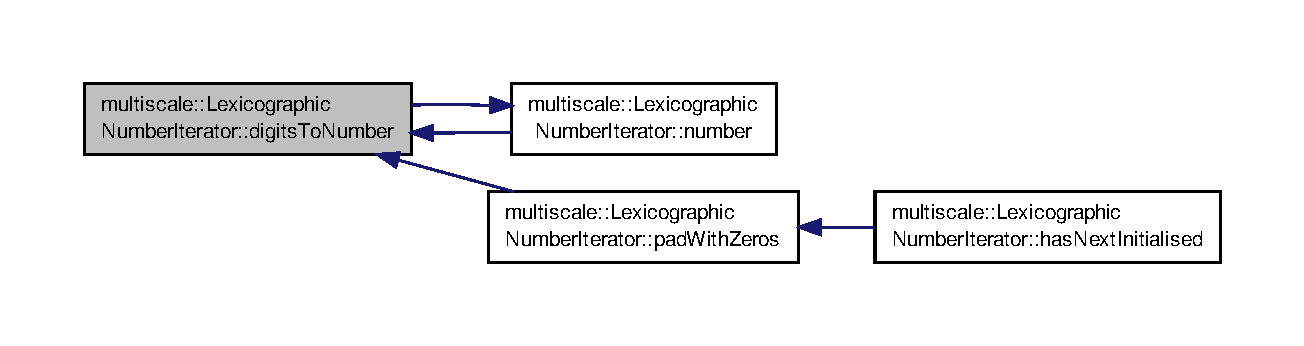
\includegraphics[width=350pt]{classmultiscale_1_1LexicographicNumberIterator_a9bcb610b3b63b02ceed7d556960e57c3_icgraph}
\end{center}
\end{figure}


\hypertarget{classmultiscale_1_1LexicographicNumberIterator_ac2754a1a57005183e2c9040719c97448}{\index{multiscale\-::\-Lexicographic\-Number\-Iterator@{multiscale\-::\-Lexicographic\-Number\-Iterator}!has\-Next\-Initialised@{has\-Next\-Initialised}}
\index{has\-Next\-Initialised@{has\-Next\-Initialised}!multiscale::LexicographicNumberIterator@{multiscale\-::\-Lexicographic\-Number\-Iterator}}
\subsubsection[{has\-Next\-Initialised}]{\setlength{\rightskip}{0pt plus 5cm}bool {\bf \-Lexicographic\-Number\-Iterator\-::has\-Next\-Initialised} (
\begin{DoxyParamCaption}
{}
\end{DoxyParamCaption}
)\hspace{0.3cm}{\ttfamily  \mbox{[}private, virtual\mbox{]}}}}\label{classmultiscale_1_1LexicographicNumberIterator_ac2754a1a57005183e2c9040719c97448}


\-Check if there is a next number when in initialised state. 



\-Implements \hyperlink{classmultiscale_1_1NumberIterator_a3c84ccdf0e279e67861b3cce34a26588}{multiscale\-::\-Number\-Iterator}.



\-Definition at line 26 of file \-Lexicographic\-Number\-Iterator.\-cpp.



\-References current\-Number\-Digits, is\-Larger\-Than\-Upper\-Bound(), and pad\-With\-Zeros().

\hypertarget{classmultiscale_1_1LexicographicNumberIterator_a943745c4723ed8c3c18df9f92bf94d2c}{\index{multiscale\-::\-Lexicographic\-Number\-Iterator@{multiscale\-::\-Lexicographic\-Number\-Iterator}!initialise@{initialise}}
\index{initialise@{initialise}!multiscale::LexicographicNumberIterator@{multiscale\-::\-Lexicographic\-Number\-Iterator}}
\subsubsection[{initialise}]{\setlength{\rightskip}{0pt plus 5cm}void {\bf \-Lexicographic\-Number\-Iterator\-::initialise} (
\begin{DoxyParamCaption}
{}
\end{DoxyParamCaption}
)\hspace{0.3cm}{\ttfamily  \mbox{[}private, virtual\mbox{]}}}}\label{classmultiscale_1_1LexicographicNumberIterator_a943745c4723ed8c3c18df9f92bf94d2c}


\-Initialise the vectors of digits. 



\-Implements \hyperlink{classmultiscale_1_1NumberIterator_a0bfeef7c3f120a5ae8d49d89b4529d6e}{multiscale\-::\-Number\-Iterator}.



\-Definition at line 20 of file \-Lexicographic\-Number\-Iterator.\-cpp.



\-References current\-Number\-Digits, number\-To\-Digits(), multiscale\-::\-Number\-Iterator\-::upper\-Bound, and upper\-Bound\-Digits.



\-Referenced by \-Lexicographic\-Number\-Iterator().



\-Here is the caller graph for this function\-:
\nopagebreak
\begin{figure}[H]
\begin{center}
\leavevmode
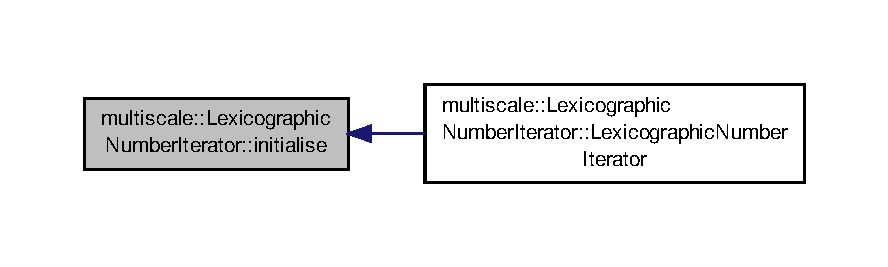
\includegraphics[width=350pt]{classmultiscale_1_1LexicographicNumberIterator_a943745c4723ed8c3c18df9f92bf94d2c_icgraph}
\end{center}
\end{figure}


\hypertarget{classmultiscale_1_1LexicographicNumberIterator_a8fad6e84a483cee3bd52c926de73d15f}{\index{multiscale\-::\-Lexicographic\-Number\-Iterator@{multiscale\-::\-Lexicographic\-Number\-Iterator}!is\-Larger\-Than\-Upper\-Bound@{is\-Larger\-Than\-Upper\-Bound}}
\index{is\-Larger\-Than\-Upper\-Bound@{is\-Larger\-Than\-Upper\-Bound}!multiscale::LexicographicNumberIterator@{multiscale\-::\-Lexicographic\-Number\-Iterator}}
\subsubsection[{is\-Larger\-Than\-Upper\-Bound}]{\setlength{\rightskip}{0pt plus 5cm}bool {\bf \-Lexicographic\-Number\-Iterator\-::is\-Larger\-Than\-Upper\-Bound} (
\begin{DoxyParamCaption}
\item[{unsigned char}]{last\-Digit}
\end{DoxyParamCaption}
)\hspace{0.3cm}{\ttfamily  \mbox{[}private\mbox{]}}}}\label{classmultiscale_1_1LexicographicNumberIterator_a8fad6e84a483cee3bd52c926de73d15f}


\-Check if the current number with the provided last digit is greater than the upper bound. 

\-Check if the current number is greater than the upper bound when replacing the last digit of the current number with the provided digit


\begin{DoxyParams}{\-Parameters}
{\em last\-Digit} & \-The last digit \\
\hline
\end{DoxyParams}


\-Definition at line 86 of file \-Lexicographic\-Number\-Iterator.\-cpp.



\-References current\-Number\-Digits, and upper\-Bound\-Digits.



\-Referenced by has\-Next\-Initialised().



\-Here is the caller graph for this function\-:
\nopagebreak
\begin{figure}[H]
\begin{center}
\leavevmode
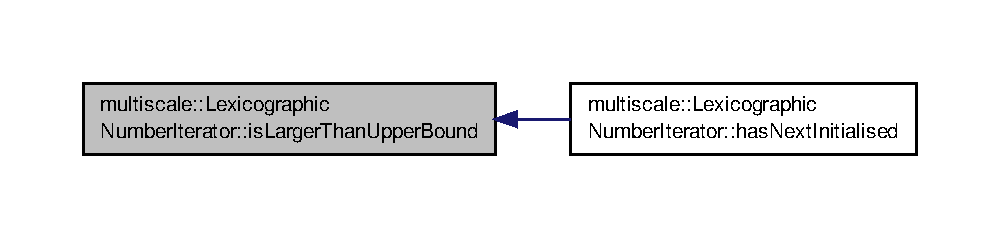
\includegraphics[width=350pt]{classmultiscale_1_1LexicographicNumberIterator_a8fad6e84a483cee3bd52c926de73d15f_icgraph}
\end{center}
\end{figure}


\hypertarget{classmultiscale_1_1LexicographicNumberIterator_a282d970d0d1a33d2736bbdf104c18336}{\index{multiscale\-::\-Lexicographic\-Number\-Iterator@{multiscale\-::\-Lexicographic\-Number\-Iterator}!number@{number}}
\index{number@{number}!multiscale::LexicographicNumberIterator@{multiscale\-::\-Lexicographic\-Number\-Iterator}}
\subsubsection[{number}]{\setlength{\rightskip}{0pt plus 5cm}unsigned int {\bf \-Lexicographic\-Number\-Iterator\-::number} (
\begin{DoxyParamCaption}
{}
\end{DoxyParamCaption}
)\hspace{0.3cm}{\ttfamily  \mbox{[}virtual\mbox{]}}}}\label{classmultiscale_1_1LexicographicNumberIterator_a282d970d0d1a33d2736bbdf104c18336}


\-Get the number pointed by the iterator. 



\-Implements \hyperlink{classmultiscale_1_1NumberIterator_a967fc14523f8726d5d6352d4ed6439ca}{multiscale\-::\-Number\-Iterator}.



\-Definition at line 16 of file \-Lexicographic\-Number\-Iterator.\-cpp.



\-References current\-Number\-Digits, and digits\-To\-Number().



\-Referenced by digits\-To\-Number(), and main().



\-Here is the caller graph for this function\-:
\nopagebreak
\begin{figure}[H]
\begin{center}
\leavevmode
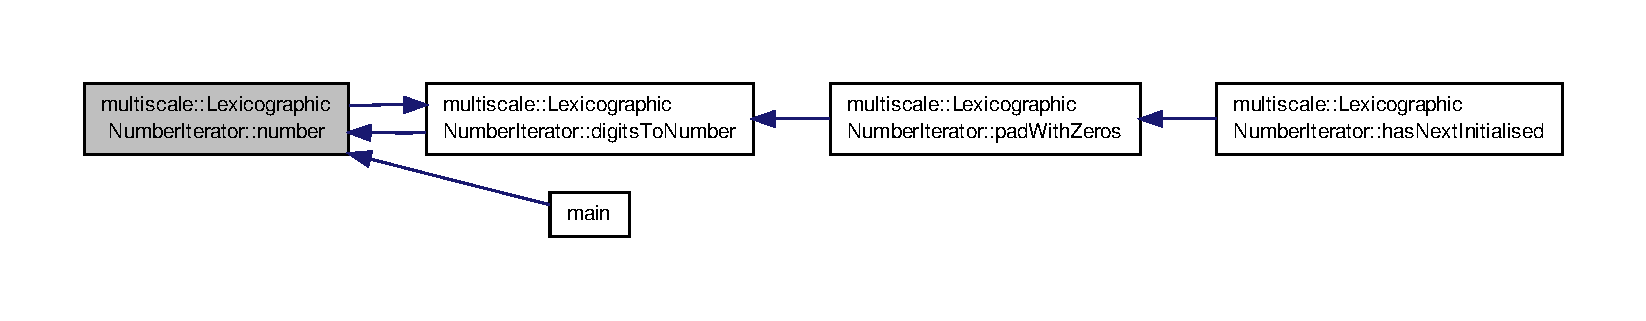
\includegraphics[width=350pt]{classmultiscale_1_1LexicographicNumberIterator_a282d970d0d1a33d2736bbdf104c18336_icgraph}
\end{center}
\end{figure}


\hypertarget{classmultiscale_1_1LexicographicNumberIterator_a700e18593ba0cc764d4e517993bd3fdc}{\index{multiscale\-::\-Lexicographic\-Number\-Iterator@{multiscale\-::\-Lexicographic\-Number\-Iterator}!number\-To\-Digits@{number\-To\-Digits}}
\index{number\-To\-Digits@{number\-To\-Digits}!multiscale::LexicographicNumberIterator@{multiscale\-::\-Lexicographic\-Number\-Iterator}}
\subsubsection[{number\-To\-Digits}]{\setlength{\rightskip}{0pt plus 5cm}void {\bf \-Lexicographic\-Number\-Iterator\-::number\-To\-Digits} (
\begin{DoxyParamCaption}
\item[{unsigned int}]{number, }
\item[{vector$<$ unsigned char $>$ \&}]{digits}
\end{DoxyParamCaption}
)\hspace{0.3cm}{\ttfamily  \mbox{[}private\mbox{]}}}}\label{classmultiscale_1_1LexicographicNumberIterator_a700e18593ba0cc764d4e517993bd3fdc}


\-Convert the number to a vector of digits. 


\begin{DoxyParams}{\-Parameters}
{\em number} & \-The number \\
\hline
{\em digits} & \-The digits of the number \\
\hline
\end{DoxyParams}


\-Definition at line 53 of file \-Lexicographic\-Number\-Iterator.\-cpp.



\-References reverse\-Digits().



\-Referenced by initialise().



\-Here is the caller graph for this function\-:
\nopagebreak
\begin{figure}[H]
\begin{center}
\leavevmode
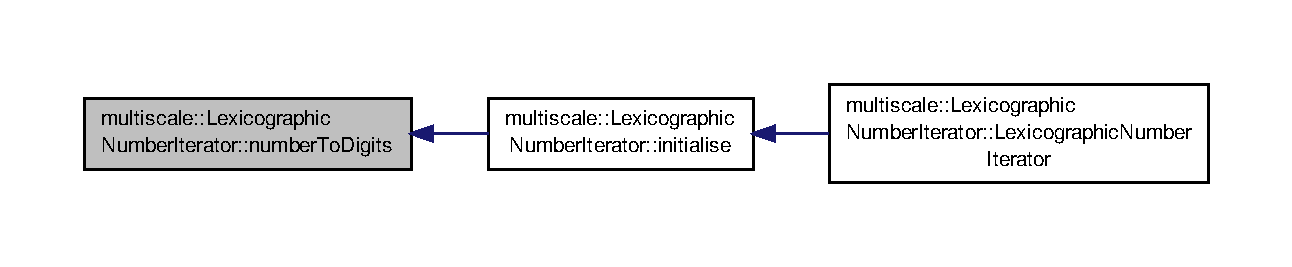
\includegraphics[width=350pt]{classmultiscale_1_1LexicographicNumberIterator_a700e18593ba0cc764d4e517993bd3fdc_icgraph}
\end{center}
\end{figure}


\hypertarget{classmultiscale_1_1LexicographicNumberIterator_a063dc7e6097724e96ed36bab4d20871b}{\index{multiscale\-::\-Lexicographic\-Number\-Iterator@{multiscale\-::\-Lexicographic\-Number\-Iterator}!pad\-With\-Zeros@{pad\-With\-Zeros}}
\index{pad\-With\-Zeros@{pad\-With\-Zeros}!multiscale::LexicographicNumberIterator@{multiscale\-::\-Lexicographic\-Number\-Iterator}}
\subsubsection[{pad\-With\-Zeros}]{\setlength{\rightskip}{0pt plus 5cm}void {\bf \-Lexicographic\-Number\-Iterator\-::pad\-With\-Zeros} (
\begin{DoxyParamCaption}
{}
\end{DoxyParamCaption}
)\hspace{0.3cm}{\ttfamily  \mbox{[}private\mbox{]}}}}\label{classmultiscale_1_1LexicographicNumberIterator_a063dc7e6097724e96ed36bab4d20871b}


\-Pad the current number with zeros. 

\-Pad the current number with the maximum number of zeros such that it does not to become larger than the upper bound 

\-Definition at line 107 of file \-Lexicographic\-Number\-Iterator.\-cpp.



\-References current\-Number\-Digits, digits\-To\-Number(), multiscale\-::\-Number\-Iterator\-::upper\-Bound, and upper\-Bound\-Digits.



\-Referenced by has\-Next\-Initialised().



\-Here is the caller graph for this function\-:
\nopagebreak
\begin{figure}[H]
\begin{center}
\leavevmode
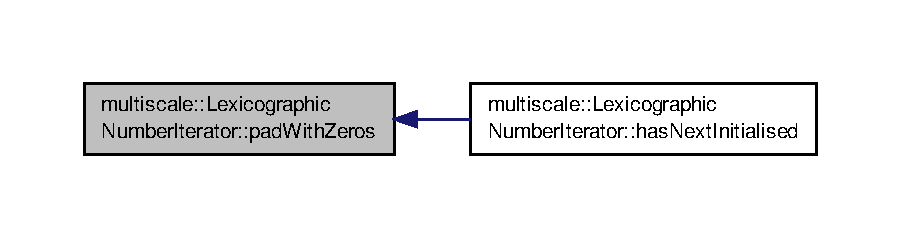
\includegraphics[width=350pt]{classmultiscale_1_1LexicographicNumberIterator_a063dc7e6097724e96ed36bab4d20871b_icgraph}
\end{center}
\end{figure}


\hypertarget{classmultiscale_1_1LexicographicNumberIterator_a18311f68a49156a415c817a947abcd7d}{\index{multiscale\-::\-Lexicographic\-Number\-Iterator@{multiscale\-::\-Lexicographic\-Number\-Iterator}!reset\-Current\-Number@{reset\-Current\-Number}}
\index{reset\-Current\-Number@{reset\-Current\-Number}!multiscale::LexicographicNumberIterator@{multiscale\-::\-Lexicographic\-Number\-Iterator}}
\subsubsection[{reset\-Current\-Number}]{\setlength{\rightskip}{0pt plus 5cm}void {\bf \-Lexicographic\-Number\-Iterator\-::reset\-Current\-Number} (
\begin{DoxyParamCaption}
{}
\end{DoxyParamCaption}
)\hspace{0.3cm}{\ttfamily  \mbox{[}private, virtual\mbox{]}}}}\label{classmultiscale_1_1LexicographicNumberIterator_a18311f68a49156a415c817a947abcd7d}


\-Reset the digits of the current number to the initial value. 



\-Implements \hyperlink{classmultiscale_1_1NumberIterator_a21e658de178b6c957df5ea0482e6fbd6}{multiscale\-::\-Number\-Iterator}.



\-Definition at line 42 of file \-Lexicographic\-Number\-Iterator.\-cpp.



\-References current\-Number\-Digits, and upper\-Bound\-Digits.

\hypertarget{classmultiscale_1_1LexicographicNumberIterator_a4c0a17e03a12256584d9ed3ae19a78c9}{\index{multiscale\-::\-Lexicographic\-Number\-Iterator@{multiscale\-::\-Lexicographic\-Number\-Iterator}!reverse\-Digits@{reverse\-Digits}}
\index{reverse\-Digits@{reverse\-Digits}!multiscale::LexicographicNumberIterator@{multiscale\-::\-Lexicographic\-Number\-Iterator}}
\subsubsection[{reverse\-Digits}]{\setlength{\rightskip}{0pt plus 5cm}void {\bf \-Lexicographic\-Number\-Iterator\-::reverse\-Digits} (
\begin{DoxyParamCaption}
\item[{vector$<$ unsigned char $>$ \&}]{digits}
\end{DoxyParamCaption}
)\hspace{0.3cm}{\ttfamily  \mbox{[}private\mbox{]}}}}\label{classmultiscale_1_1LexicographicNumberIterator_a4c0a17e03a12256584d9ed3ae19a78c9}


\-Reverse the order of the digits. 

\-Reverse the order of the digits such that the first one is swapped with the last one, the second one is swapped with the last but one and so on.


\begin{DoxyParams}{\-Parameters}
{\em digits} & \-The digits \\
\hline
\end{DoxyParams}


\-Definition at line 63 of file \-Lexicographic\-Number\-Iterator.\-cpp.



\-Referenced by number\-To\-Digits().



\-Here is the caller graph for this function\-:
\nopagebreak
\begin{figure}[H]
\begin{center}
\leavevmode
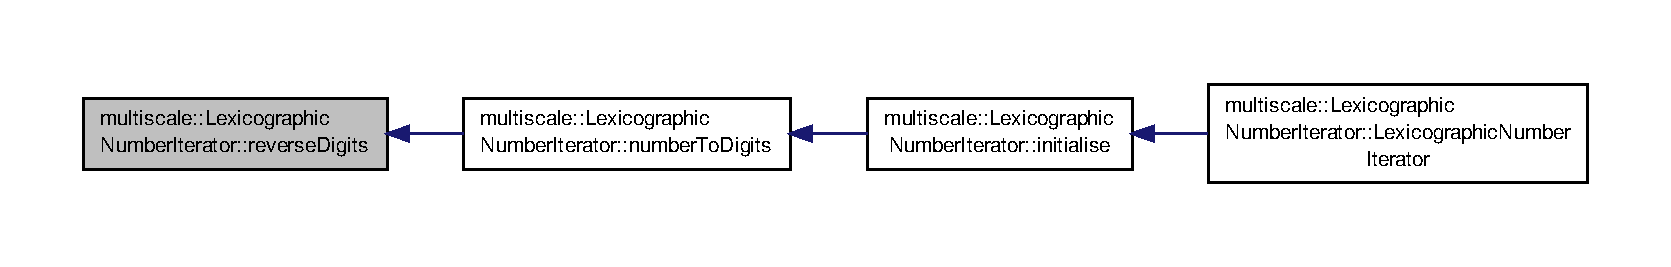
\includegraphics[width=350pt]{classmultiscale_1_1LexicographicNumberIterator_a4c0a17e03a12256584d9ed3ae19a78c9_icgraph}
\end{center}
\end{figure}




\subsection{\-Member \-Data \-Documentation}
\hypertarget{classmultiscale_1_1LexicographicNumberIterator_af42ebeea695a31c2da714332c520ae79}{\index{multiscale\-::\-Lexicographic\-Number\-Iterator@{multiscale\-::\-Lexicographic\-Number\-Iterator}!current\-Number\-Digits@{current\-Number\-Digits}}
\index{current\-Number\-Digits@{current\-Number\-Digits}!multiscale::LexicographicNumberIterator@{multiscale\-::\-Lexicographic\-Number\-Iterator}}
\subsubsection[{current\-Number\-Digits}]{\setlength{\rightskip}{0pt plus 5cm}vector$<$unsigned char$>$ {\bf multiscale\-::\-Lexicographic\-Number\-Iterator\-::current\-Number\-Digits}\hspace{0.3cm}{\ttfamily  \mbox{[}private\mbox{]}}}}\label{classmultiscale_1_1LexicographicNumberIterator_af42ebeea695a31c2da714332c520ae79}
\-The digits of the number to which the iterator points 

\-Definition at line 19 of file \-Lexicographic\-Number\-Iterator.\-hpp.



\-Referenced by has\-Next\-Initialised(), initialise(), is\-Larger\-Than\-Upper\-Bound(), number(), pad\-With\-Zeros(), reset\-Current\-Number(), and $\sim$\-Lexicographic\-Number\-Iterator().

\hypertarget{classmultiscale_1_1LexicographicNumberIterator_a909a054ae4d3e79e5daa3059a94000d0}{\index{multiscale\-::\-Lexicographic\-Number\-Iterator@{multiscale\-::\-Lexicographic\-Number\-Iterator}!upper\-Bound\-Digits@{upper\-Bound\-Digits}}
\index{upper\-Bound\-Digits@{upper\-Bound\-Digits}!multiscale::LexicographicNumberIterator@{multiscale\-::\-Lexicographic\-Number\-Iterator}}
\subsubsection[{upper\-Bound\-Digits}]{\setlength{\rightskip}{0pt plus 5cm}vector$<$unsigned char$>$ {\bf multiscale\-::\-Lexicographic\-Number\-Iterator\-::upper\-Bound\-Digits}\hspace{0.3cm}{\ttfamily  \mbox{[}private\mbox{]}}}}\label{classmultiscale_1_1LexicographicNumberIterator_a909a054ae4d3e79e5daa3059a94000d0}
\-The digits of the upper bound 

\-Definition at line 18 of file \-Lexicographic\-Number\-Iterator.\-hpp.



\-Referenced by initialise(), is\-Larger\-Than\-Upper\-Bound(), pad\-With\-Zeros(), reset\-Current\-Number(), and $\sim$\-Lexicographic\-Number\-Iterator().



\-The documentation for this class was generated from the following files\-:\begin{DoxyCompactItemize}
\item 
/home/ovidiu/\-Repositories/git/multiscale/\-Multiscale/modules/util/include/multiscale/util/iterator/\hyperlink{LexicographicNumberIterator_8hpp}{\-Lexicographic\-Number\-Iterator.\-hpp}\item 
/home/ovidiu/\-Repositories/git/multiscale/\-Multiscale/modules/util/src/iterator/\hyperlink{LexicographicNumberIterator_8cpp}{\-Lexicographic\-Number\-Iterator.\-cpp}\end{DoxyCompactItemize}

\hypertarget{classmultiscale_1_1analysis_1_1MatFactory}{\section{multiscale\-:\-:analysis\-:\-:Mat\-Factory Class Reference}
\label{classmultiscale_1_1analysis_1_1MatFactory}\index{multiscale\-::analysis\-::\-Mat\-Factory@{multiscale\-::analysis\-::\-Mat\-Factory}}
}


Class for creating a Mat object.  




{\ttfamily \#include $<$Mat\-Factory.\-hpp$>$}



Inheritance diagram for multiscale\-:\-:analysis\-:\-:Mat\-Factory\-:
\nopagebreak
\begin{figure}[H]
\begin{center}
\leavevmode
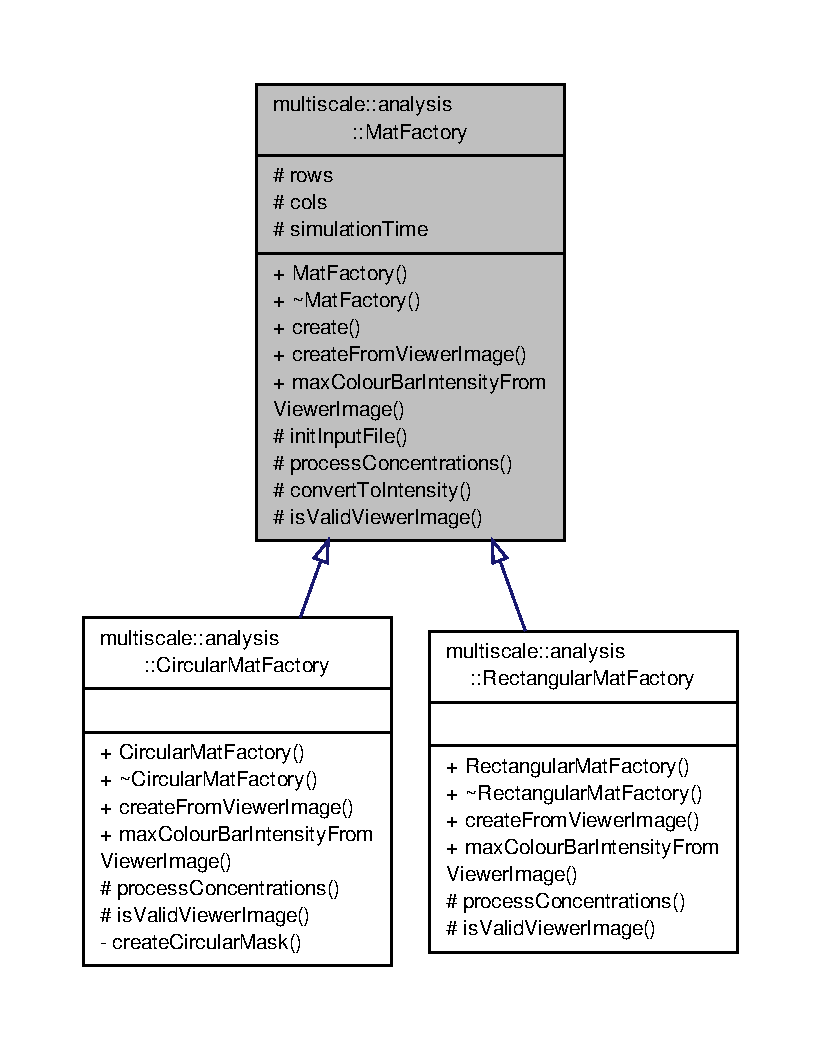
\includegraphics[width=350pt]{classmultiscale_1_1analysis_1_1MatFactory__inherit__graph}
\end{center}
\end{figure}


Collaboration diagram for multiscale\-:\-:analysis\-:\-:Mat\-Factory\-:
\nopagebreak
\begin{figure}[H]
\begin{center}
\leavevmode
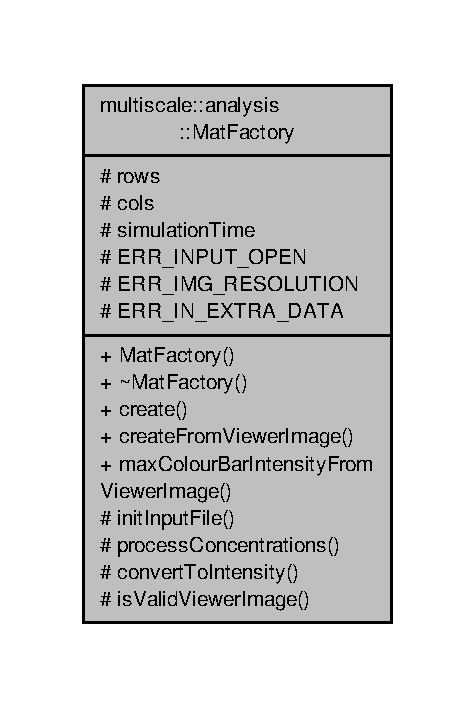
\includegraphics[width=228pt]{classmultiscale_1_1analysis_1_1MatFactory__coll__graph}
\end{center}
\end{figure}
\subsection*{Public Member Functions}
\begin{DoxyCompactItemize}
\item 
\hyperlink{classmultiscale_1_1analysis_1_1MatFactory_a454ca2abfbeb664e75f5365ac00eacff}{Mat\-Factory} ()
\item 
virtual \hyperlink{classmultiscale_1_1analysis_1_1MatFactory_aa339532cb504caebcf9ece2c847f4847}{$\sim$\-Mat\-Factory} ()
\item 
Mat \hyperlink{classmultiscale_1_1analysis_1_1MatFactory_a7800a989d808037fe96a9d5a692909b0}{create} (const string \&input\-File)
\begin{DoxyCompactList}\small\item\em Create a Mat object from the input file. \end{DoxyCompactList}\item 
virtual Mat \hyperlink{classmultiscale_1_1analysis_1_1MatFactory_a719ca9ac925ee182c1d5df1b0b029394}{create\-From\-Viewer\-Image} (const string \&input\-File)=0
\begin{DoxyCompactList}\small\item\em Create a Mat object from the image file obtained from Rectangular/\-Circular\-Geometry\-Viewer. \end{DoxyCompactList}\item 
virtual double \hyperlink{classmultiscale_1_1analysis_1_1MatFactory_a041b354357794476a2108e3f71deadc8}{max\-Colour\-Bar\-Intensity\-From\-Viewer\-Image} (const string \&input\-File)=0
\begin{DoxyCompactList}\small\item\em Get the maximum grayscale intensity of the colour bar in the image. \end{DoxyCompactList}\end{DoxyCompactItemize}
\subsection*{Protected Member Functions}
\begin{DoxyCompactItemize}
\item 
void \hyperlink{classmultiscale_1_1analysis_1_1MatFactory_a7b54550119d9a44708dad9c1c4eefc7e}{init\-Input\-File} (ifstream \&fin, const string \&input\-File)
\begin{DoxyCompactList}\small\item\em Initialise the input file. \end{DoxyCompactList}\item 
virtual unsigned char $\ast$ \hyperlink{classmultiscale_1_1analysis_1_1MatFactory_a0493c87d7b74619a95f14c0e31a3e178}{process\-Concentrations} (ifstream \&fin)=0
\begin{DoxyCompactList}\small\item\em Process concentrations from file. \end{DoxyCompactList}\item 
unsigned char \hyperlink{classmultiscale_1_1analysis_1_1MatFactory_a015bb6710f3a832786d7291108323696}{convert\-To\-Intensity} (double concentration)
\begin{DoxyCompactList}\small\item\em Convert concentration to intensity. \end{DoxyCompactList}\item 
virtual bool \hyperlink{classmultiscale_1_1analysis_1_1MatFactory_ad6acdd120b128eb9fb502fca23a7de69}{is\-Valid\-Viewer\-Image} (const Mat \&image)=0
\begin{DoxyCompactList}\small\item\em Check if the image generated by the viewer has the required resolution. \end{DoxyCompactList}\end{DoxyCompactItemize}
\subsection*{Protected Attributes}
\begin{DoxyCompactItemize}
\item 
int \hyperlink{classmultiscale_1_1analysis_1_1MatFactory_a35672fb0c992f662018ee7c146794474}{rows}
\item 
int \hyperlink{classmultiscale_1_1analysis_1_1MatFactory_a9514356fe5226eaa31a4e61ca62a027c}{cols}
\item 
double \hyperlink{classmultiscale_1_1analysis_1_1MatFactory_a99caa620805ac50375699236d83fbd96}{simulation\-Time}
\end{DoxyCompactItemize}
\subsection*{Static Protected Attributes}
\begin{DoxyCompactItemize}
\item 
static const string \hyperlink{classmultiscale_1_1analysis_1_1MatFactory_a06de250e466b41fcca4fa61a52a575fc}{E\-R\-R\-\_\-\-I\-N\-P\-U\-T\-\_\-\-O\-P\-E\-N} = \char`\"{}The input file could not be opened.\char`\"{}
\item 
static const string \hyperlink{classmultiscale_1_1analysis_1_1MatFactory_ab5e9403dc7f8465189d444f909d473e7}{E\-R\-R\-\_\-\-I\-M\-G\-\_\-\-R\-E\-S\-O\-L\-U\-T\-I\-O\-N} = \char`\"{}The resolution of the input image is not the expected one.\char`\"{}
\item 
static const string \hyperlink{classmultiscale_1_1analysis_1_1MatFactory_a09459b632d5b01f184ce0f56245f5905}{E\-R\-R\-\_\-\-I\-N\-\_\-\-E\-X\-T\-R\-A\-\_\-\-D\-A\-T\-A} = \char`\"{}The input file contains more data than required.\char`\"{}
\end{DoxyCompactItemize}


\subsection{Detailed Description}
Class for creating a Mat object. 

Definition at line 16 of file Mat\-Factory.\-hpp.



\subsection{Constructor \& Destructor Documentation}
\hypertarget{classmultiscale_1_1analysis_1_1MatFactory_a454ca2abfbeb664e75f5365ac00eacff}{\index{multiscale\-::analysis\-::\-Mat\-Factory@{multiscale\-::analysis\-::\-Mat\-Factory}!Mat\-Factory@{Mat\-Factory}}
\index{Mat\-Factory@{Mat\-Factory}!multiscale::analysis::MatFactory@{multiscale\-::analysis\-::\-Mat\-Factory}}
\subsubsection[{Mat\-Factory}]{\setlength{\rightskip}{0pt plus 5cm}Mat\-Factory\-::\-Mat\-Factory (
\begin{DoxyParamCaption}
{}
\end{DoxyParamCaption}
)}}\label{classmultiscale_1_1analysis_1_1MatFactory_a454ca2abfbeb664e75f5365ac00eacff}


Definition at line 9 of file Mat\-Factory.\-cpp.

\hypertarget{classmultiscale_1_1analysis_1_1MatFactory_aa339532cb504caebcf9ece2c847f4847}{\index{multiscale\-::analysis\-::\-Mat\-Factory@{multiscale\-::analysis\-::\-Mat\-Factory}!$\sim$\-Mat\-Factory@{$\sim$\-Mat\-Factory}}
\index{$\sim$\-Mat\-Factory@{$\sim$\-Mat\-Factory}!multiscale::analysis::MatFactory@{multiscale\-::analysis\-::\-Mat\-Factory}}
\subsubsection[{$\sim$\-Mat\-Factory}]{\setlength{\rightskip}{0pt plus 5cm}Mat\-Factory\-::$\sim$\-Mat\-Factory (
\begin{DoxyParamCaption}
{}
\end{DoxyParamCaption}
)\hspace{0.3cm}{\ttfamily [virtual]}}}\label{classmultiscale_1_1analysis_1_1MatFactory_aa339532cb504caebcf9ece2c847f4847}


Definition at line 11 of file Mat\-Factory.\-cpp.



\subsection{Member Function Documentation}
\hypertarget{classmultiscale_1_1analysis_1_1MatFactory_a015bb6710f3a832786d7291108323696}{\index{multiscale\-::analysis\-::\-Mat\-Factory@{multiscale\-::analysis\-::\-Mat\-Factory}!convert\-To\-Intensity@{convert\-To\-Intensity}}
\index{convert\-To\-Intensity@{convert\-To\-Intensity}!multiscale::analysis::MatFactory@{multiscale\-::analysis\-::\-Mat\-Factory}}
\subsubsection[{convert\-To\-Intensity}]{\setlength{\rightskip}{0pt plus 5cm}unsigned char Mat\-Factory\-::convert\-To\-Intensity (
\begin{DoxyParamCaption}
\item[{double}]{concentration}
\end{DoxyParamCaption}
)\hspace{0.3cm}{\ttfamily [protected]}}}\label{classmultiscale_1_1analysis_1_1MatFactory_a015bb6710f3a832786d7291108323696}


Convert concentration to intensity. 

Convert the concentration (real value between 0 and 1) to intensity (integer value between 0 and 255)


\begin{DoxyParams}{Parameters}
{\em concentration} & A value between 0 and 1 \\
\hline
\end{DoxyParams}


Definition at line 43 of file Mat\-Factory.\-cpp.



Referenced by multiscale\-::analysis\-::\-Rectangular\-Mat\-Factory\-::process\-Concentrations().



Here is the caller graph for this function\-:\nopagebreak
\begin{figure}[H]
\begin{center}
\leavevmode
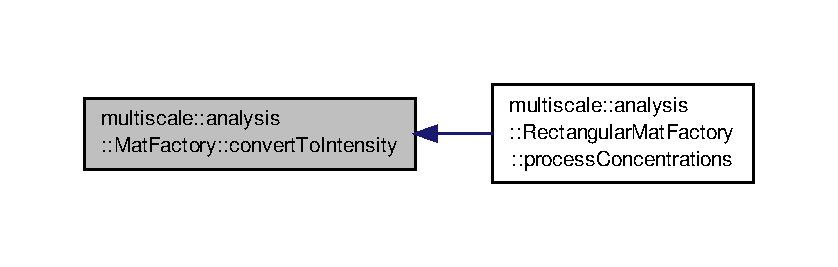
\includegraphics[width=350pt]{classmultiscale_1_1analysis_1_1MatFactory_a015bb6710f3a832786d7291108323696_icgraph}
\end{center}
\end{figure}


\hypertarget{classmultiscale_1_1analysis_1_1MatFactory_a7800a989d808037fe96a9d5a692909b0}{\index{multiscale\-::analysis\-::\-Mat\-Factory@{multiscale\-::analysis\-::\-Mat\-Factory}!create@{create}}
\index{create@{create}!multiscale::analysis::MatFactory@{multiscale\-::analysis\-::\-Mat\-Factory}}
\subsubsection[{create}]{\setlength{\rightskip}{0pt plus 5cm}Mat Mat\-Factory\-::create (
\begin{DoxyParamCaption}
\item[{const string \&}]{input\-File}
\end{DoxyParamCaption}
)}}\label{classmultiscale_1_1analysis_1_1MatFactory_a7800a989d808037fe96a9d5a692909b0}


Create a Mat object from the input file. 

Create the Mat instance from the values given in the input file

F\-O\-R\-M\-A\-T O\-F I\-N\-P\-U\-T F\-I\-L\-E\-:
\begin{DoxyItemize}
\item 1st line contains two positive integers and a real value\-: nr\-\_\-rows, nr\-\_\-cols and simulation\-\_\-time
\item 2nd -\/ (nr\-\_\-rows + 1)th lines contain the concentrations of the positions in the grid
\end{DoxyItemize}


\begin{DoxyParams}{Parameters}
{\em input\-File} & The path to the input file \\
\hline
\end{DoxyParams}


Definition at line 13 of file Mat\-Factory.\-cpp.



References cols, E\-R\-R\-\_\-\-I\-N\-\_\-\-E\-X\-T\-R\-A\-\_\-\-D\-A\-T\-A, init\-Input\-File(), M\-S\-\_\-throw, process\-Concentrations(), and rows.



Here is the call graph for this function\-:\nopagebreak
\begin{figure}[H]
\begin{center}
\leavevmode
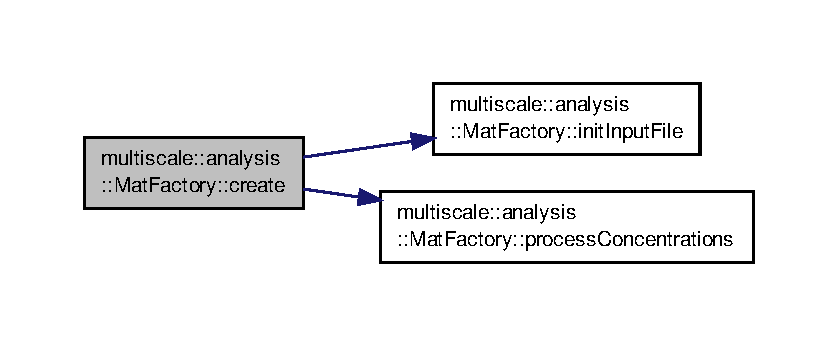
\includegraphics[width=350pt]{classmultiscale_1_1analysis_1_1MatFactory_a7800a989d808037fe96a9d5a692909b0_cgraph}
\end{center}
\end{figure}


\hypertarget{classmultiscale_1_1analysis_1_1MatFactory_a719ca9ac925ee182c1d5df1b0b029394}{\index{multiscale\-::analysis\-::\-Mat\-Factory@{multiscale\-::analysis\-::\-Mat\-Factory}!create\-From\-Viewer\-Image@{create\-From\-Viewer\-Image}}
\index{create\-From\-Viewer\-Image@{create\-From\-Viewer\-Image}!multiscale::analysis::MatFactory@{multiscale\-::analysis\-::\-Mat\-Factory}}
\subsubsection[{create\-From\-Viewer\-Image}]{\setlength{\rightskip}{0pt plus 5cm}virtual Mat multiscale\-::analysis\-::\-Mat\-Factory\-::create\-From\-Viewer\-Image (
\begin{DoxyParamCaption}
\item[{const string \&}]{input\-File}
\end{DoxyParamCaption}
)\hspace{0.3cm}{\ttfamily [pure virtual]}}}\label{classmultiscale_1_1analysis_1_1MatFactory_a719ca9ac925ee182c1d5df1b0b029394}


Create a Mat object from the image file obtained from Rectangular/\-Circular\-Geometry\-Viewer. 

Create the Mat instance from the given image file


\begin{DoxyParams}{Parameters}
{\em input\-File} & The path to the image file \\
\hline
\end{DoxyParams}


Implemented in \hyperlink{classmultiscale_1_1analysis_1_1CircularMatFactory_a8d5fccf946065b982bfa700b9e47b1f5}{multiscale\-::analysis\-::\-Circular\-Mat\-Factory}, and \hyperlink{classmultiscale_1_1analysis_1_1RectangularMatFactory_a3f86c9bd73eb8d8a27f272b47e984871}{multiscale\-::analysis\-::\-Rectangular\-Mat\-Factory}.

\hypertarget{classmultiscale_1_1analysis_1_1MatFactory_a7b54550119d9a44708dad9c1c4eefc7e}{\index{multiscale\-::analysis\-::\-Mat\-Factory@{multiscale\-::analysis\-::\-Mat\-Factory}!init\-Input\-File@{init\-Input\-File}}
\index{init\-Input\-File@{init\-Input\-File}!multiscale::analysis::MatFactory@{multiscale\-::analysis\-::\-Mat\-Factory}}
\subsubsection[{init\-Input\-File}]{\setlength{\rightskip}{0pt plus 5cm}void Mat\-Factory\-::init\-Input\-File (
\begin{DoxyParamCaption}
\item[{ifstream \&}]{fin, }
\item[{const string \&}]{input\-File}
\end{DoxyParamCaption}
)\hspace{0.3cm}{\ttfamily [protected]}}}\label{classmultiscale_1_1analysis_1_1MatFactory_a7b54550119d9a44708dad9c1c4eefc7e}


Initialise the input file. 

Initialise the input file. Open an input file stream to the given input file path.


\begin{DoxyParams}{Parameters}
{\em fin} & An input stream for reading data from the input file \\
\hline
{\em input\-File} & The path to the input file \\
\hline
\end{DoxyParams}


Definition at line 33 of file Mat\-Factory.\-cpp.



References cols, E\-R\-R\-\_\-\-I\-N\-P\-U\-T\-\_\-\-O\-P\-E\-N, M\-S\-\_\-throw, rows, and simulation\-Time.



Referenced by create().



Here is the caller graph for this function\-:\nopagebreak
\begin{figure}[H]
\begin{center}
\leavevmode
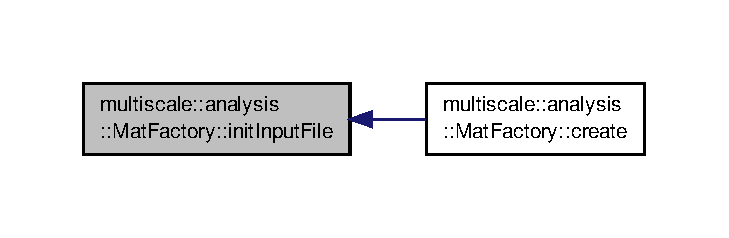
\includegraphics[width=350pt]{classmultiscale_1_1analysis_1_1MatFactory_a7b54550119d9a44708dad9c1c4eefc7e_icgraph}
\end{center}
\end{figure}


\hypertarget{classmultiscale_1_1analysis_1_1MatFactory_ad6acdd120b128eb9fb502fca23a7de69}{\index{multiscale\-::analysis\-::\-Mat\-Factory@{multiscale\-::analysis\-::\-Mat\-Factory}!is\-Valid\-Viewer\-Image@{is\-Valid\-Viewer\-Image}}
\index{is\-Valid\-Viewer\-Image@{is\-Valid\-Viewer\-Image}!multiscale::analysis::MatFactory@{multiscale\-::analysis\-::\-Mat\-Factory}}
\subsubsection[{is\-Valid\-Viewer\-Image}]{\setlength{\rightskip}{0pt plus 5cm}virtual bool multiscale\-::analysis\-::\-Mat\-Factory\-::is\-Valid\-Viewer\-Image (
\begin{DoxyParamCaption}
\item[{const Mat \&}]{image}
\end{DoxyParamCaption}
)\hspace{0.3cm}{\ttfamily [protected]}, {\ttfamily [pure virtual]}}}\label{classmultiscale_1_1analysis_1_1MatFactory_ad6acdd120b128eb9fb502fca23a7de69}


Check if the image generated by the viewer has the required resolution. 


\begin{DoxyParams}{Parameters}
{\em image} & Image generated by the viewer \\
\hline
\end{DoxyParams}


Implemented in \hyperlink{classmultiscale_1_1analysis_1_1RectangularMatFactory_a398913bbfa8ca9d80cb630c29a37a135}{multiscale\-::analysis\-::\-Rectangular\-Mat\-Factory}, and \hyperlink{classmultiscale_1_1analysis_1_1CircularMatFactory_a08e407b35a2d314c1aa17f21040ff23a}{multiscale\-::analysis\-::\-Circular\-Mat\-Factory}.

\hypertarget{classmultiscale_1_1analysis_1_1MatFactory_a041b354357794476a2108e3f71deadc8}{\index{multiscale\-::analysis\-::\-Mat\-Factory@{multiscale\-::analysis\-::\-Mat\-Factory}!max\-Colour\-Bar\-Intensity\-From\-Viewer\-Image@{max\-Colour\-Bar\-Intensity\-From\-Viewer\-Image}}
\index{max\-Colour\-Bar\-Intensity\-From\-Viewer\-Image@{max\-Colour\-Bar\-Intensity\-From\-Viewer\-Image}!multiscale::analysis::MatFactory@{multiscale\-::analysis\-::\-Mat\-Factory}}
\subsubsection[{max\-Colour\-Bar\-Intensity\-From\-Viewer\-Image}]{\setlength{\rightskip}{0pt plus 5cm}virtual double multiscale\-::analysis\-::\-Mat\-Factory\-::max\-Colour\-Bar\-Intensity\-From\-Viewer\-Image (
\begin{DoxyParamCaption}
\item[{const string \&}]{input\-File}
\end{DoxyParamCaption}
)\hspace{0.3cm}{\ttfamily [pure virtual]}}}\label{classmultiscale_1_1analysis_1_1MatFactory_a041b354357794476a2108e3f71deadc8}


Get the maximum grayscale intensity of the colour bar in the image. 


\begin{DoxyParams}{Parameters}
{\em input\-File} & The path to the image file \\
\hline
\end{DoxyParams}


Implemented in \hyperlink{classmultiscale_1_1analysis_1_1CircularMatFactory_aea41720f6adfb983bb94ea0a45789874}{multiscale\-::analysis\-::\-Circular\-Mat\-Factory}, and \hyperlink{classmultiscale_1_1analysis_1_1RectangularMatFactory_a9255b11748b4c48d76c769258d6b6ee0}{multiscale\-::analysis\-::\-Rectangular\-Mat\-Factory}.

\hypertarget{classmultiscale_1_1analysis_1_1MatFactory_a0493c87d7b74619a95f14c0e31a3e178}{\index{multiscale\-::analysis\-::\-Mat\-Factory@{multiscale\-::analysis\-::\-Mat\-Factory}!process\-Concentrations@{process\-Concentrations}}
\index{process\-Concentrations@{process\-Concentrations}!multiscale::analysis::MatFactory@{multiscale\-::analysis\-::\-Mat\-Factory}}
\subsubsection[{process\-Concentrations}]{\setlength{\rightskip}{0pt plus 5cm}virtual unsigned char$\ast$ multiscale\-::analysis\-::\-Mat\-Factory\-::process\-Concentrations (
\begin{DoxyParamCaption}
\item[{ifstream \&}]{fin}
\end{DoxyParamCaption}
)\hspace{0.3cm}{\ttfamily [protected]}, {\ttfamily [pure virtual]}}}\label{classmultiscale_1_1analysis_1_1MatFactory_a0493c87d7b74619a95f14c0e31a3e178}


Process concentrations from file. 

Process the concentrations from the file. This method will be implemented only by subclasses of this abstract class 

Implemented in \hyperlink{classmultiscale_1_1analysis_1_1RectangularMatFactory_a6cc84a4eadbab5046cb6eacba64f5ae4}{multiscale\-::analysis\-::\-Rectangular\-Mat\-Factory}, and \hyperlink{classmultiscale_1_1analysis_1_1CircularMatFactory_a8fe40d38b896f440e17b5514462d1e8a}{multiscale\-::analysis\-::\-Circular\-Mat\-Factory}.



Referenced by create().



Here is the caller graph for this function\-:\nopagebreak
\begin{figure}[H]
\begin{center}
\leavevmode
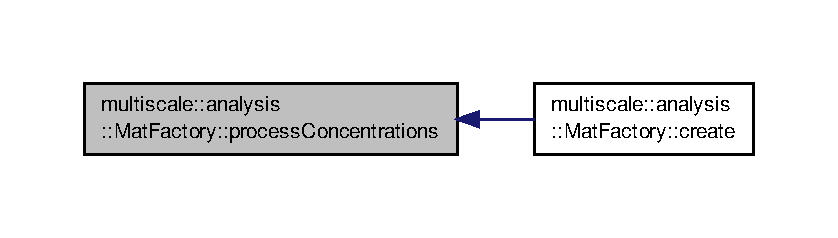
\includegraphics[width=350pt]{classmultiscale_1_1analysis_1_1MatFactory_a0493c87d7b74619a95f14c0e31a3e178_icgraph}
\end{center}
\end{figure}




\subsection{Member Data Documentation}
\hypertarget{classmultiscale_1_1analysis_1_1MatFactory_a9514356fe5226eaa31a4e61ca62a027c}{\index{multiscale\-::analysis\-::\-Mat\-Factory@{multiscale\-::analysis\-::\-Mat\-Factory}!cols@{cols}}
\index{cols@{cols}!multiscale::analysis::MatFactory@{multiscale\-::analysis\-::\-Mat\-Factory}}
\subsubsection[{cols}]{\setlength{\rightskip}{0pt plus 5cm}int multiscale\-::analysis\-::\-Mat\-Factory\-::cols\hspace{0.3cm}{\ttfamily [protected]}}}\label{classmultiscale_1_1analysis_1_1MatFactory_a9514356fe5226eaa31a4e61ca62a027c}
Number of columns in the Mat object 

Definition at line 21 of file Mat\-Factory.\-hpp.



Referenced by create(), init\-Input\-File(), and multiscale\-::analysis\-::\-Rectangular\-Mat\-Factory\-::process\-Concentrations().

\hypertarget{classmultiscale_1_1analysis_1_1MatFactory_ab5e9403dc7f8465189d444f909d473e7}{\index{multiscale\-::analysis\-::\-Mat\-Factory@{multiscale\-::analysis\-::\-Mat\-Factory}!E\-R\-R\-\_\-\-I\-M\-G\-\_\-\-R\-E\-S\-O\-L\-U\-T\-I\-O\-N@{E\-R\-R\-\_\-\-I\-M\-G\-\_\-\-R\-E\-S\-O\-L\-U\-T\-I\-O\-N}}
\index{E\-R\-R\-\_\-\-I\-M\-G\-\_\-\-R\-E\-S\-O\-L\-U\-T\-I\-O\-N@{E\-R\-R\-\_\-\-I\-M\-G\-\_\-\-R\-E\-S\-O\-L\-U\-T\-I\-O\-N}!multiscale::analysis::MatFactory@{multiscale\-::analysis\-::\-Mat\-Factory}}
\subsubsection[{E\-R\-R\-\_\-\-I\-M\-G\-\_\-\-R\-E\-S\-O\-L\-U\-T\-I\-O\-N}]{\setlength{\rightskip}{0pt plus 5cm}const string Mat\-Factory\-::\-E\-R\-R\-\_\-\-I\-M\-G\-\_\-\-R\-E\-S\-O\-L\-U\-T\-I\-O\-N = \char`\"{}The resolution of the input image is not the expected one.\char`\"{}\hspace{0.3cm}{\ttfamily [static]}, {\ttfamily [protected]}}}\label{classmultiscale_1_1analysis_1_1MatFactory_ab5e9403dc7f8465189d444f909d473e7}


Definition at line 91 of file Mat\-Factory.\-hpp.



Referenced by multiscale\-::analysis\-::\-Circular\-Mat\-Factory\-::is\-Valid\-Viewer\-Image(), and multiscale\-::analysis\-::\-Rectangular\-Mat\-Factory\-::is\-Valid\-Viewer\-Image().

\hypertarget{classmultiscale_1_1analysis_1_1MatFactory_a09459b632d5b01f184ce0f56245f5905}{\index{multiscale\-::analysis\-::\-Mat\-Factory@{multiscale\-::analysis\-::\-Mat\-Factory}!E\-R\-R\-\_\-\-I\-N\-\_\-\-E\-X\-T\-R\-A\-\_\-\-D\-A\-T\-A@{E\-R\-R\-\_\-\-I\-N\-\_\-\-E\-X\-T\-R\-A\-\_\-\-D\-A\-T\-A}}
\index{E\-R\-R\-\_\-\-I\-N\-\_\-\-E\-X\-T\-R\-A\-\_\-\-D\-A\-T\-A@{E\-R\-R\-\_\-\-I\-N\-\_\-\-E\-X\-T\-R\-A\-\_\-\-D\-A\-T\-A}!multiscale::analysis::MatFactory@{multiscale\-::analysis\-::\-Mat\-Factory}}
\subsubsection[{E\-R\-R\-\_\-\-I\-N\-\_\-\-E\-X\-T\-R\-A\-\_\-\-D\-A\-T\-A}]{\setlength{\rightskip}{0pt plus 5cm}const string Mat\-Factory\-::\-E\-R\-R\-\_\-\-I\-N\-\_\-\-E\-X\-T\-R\-A\-\_\-\-D\-A\-T\-A = \char`\"{}The input file contains more data than required.\char`\"{}\hspace{0.3cm}{\ttfamily [static]}, {\ttfamily [protected]}}}\label{classmultiscale_1_1analysis_1_1MatFactory_a09459b632d5b01f184ce0f56245f5905}


Definition at line 92 of file Mat\-Factory.\-hpp.



Referenced by create().

\hypertarget{classmultiscale_1_1analysis_1_1MatFactory_a06de250e466b41fcca4fa61a52a575fc}{\index{multiscale\-::analysis\-::\-Mat\-Factory@{multiscale\-::analysis\-::\-Mat\-Factory}!E\-R\-R\-\_\-\-I\-N\-P\-U\-T\-\_\-\-O\-P\-E\-N@{E\-R\-R\-\_\-\-I\-N\-P\-U\-T\-\_\-\-O\-P\-E\-N}}
\index{E\-R\-R\-\_\-\-I\-N\-P\-U\-T\-\_\-\-O\-P\-E\-N@{E\-R\-R\-\_\-\-I\-N\-P\-U\-T\-\_\-\-O\-P\-E\-N}!multiscale::analysis::MatFactory@{multiscale\-::analysis\-::\-Mat\-Factory}}
\subsubsection[{E\-R\-R\-\_\-\-I\-N\-P\-U\-T\-\_\-\-O\-P\-E\-N}]{\setlength{\rightskip}{0pt plus 5cm}const string Mat\-Factory\-::\-E\-R\-R\-\_\-\-I\-N\-P\-U\-T\-\_\-\-O\-P\-E\-N = \char`\"{}The input file could not be opened.\char`\"{}\hspace{0.3cm}{\ttfamily [static]}, {\ttfamily [protected]}}}\label{classmultiscale_1_1analysis_1_1MatFactory_a06de250e466b41fcca4fa61a52a575fc}


Definition at line 90 of file Mat\-Factory.\-hpp.



Referenced by init\-Input\-File(), multiscale\-::analysis\-::\-Circular\-Mat\-Factory\-::is\-Valid\-Viewer\-Image(), and multiscale\-::analysis\-::\-Rectangular\-Mat\-Factory\-::is\-Valid\-Viewer\-Image().

\hypertarget{classmultiscale_1_1analysis_1_1MatFactory_a35672fb0c992f662018ee7c146794474}{\index{multiscale\-::analysis\-::\-Mat\-Factory@{multiscale\-::analysis\-::\-Mat\-Factory}!rows@{rows}}
\index{rows@{rows}!multiscale::analysis::MatFactory@{multiscale\-::analysis\-::\-Mat\-Factory}}
\subsubsection[{rows}]{\setlength{\rightskip}{0pt plus 5cm}int multiscale\-::analysis\-::\-Mat\-Factory\-::rows\hspace{0.3cm}{\ttfamily [protected]}}}\label{classmultiscale_1_1analysis_1_1MatFactory_a35672fb0c992f662018ee7c146794474}
Number of rows in the Mat object 

Definition at line 20 of file Mat\-Factory.\-hpp.



Referenced by create(), init\-Input\-File(), and multiscale\-::analysis\-::\-Rectangular\-Mat\-Factory\-::process\-Concentrations().

\hypertarget{classmultiscale_1_1analysis_1_1MatFactory_a99caa620805ac50375699236d83fbd96}{\index{multiscale\-::analysis\-::\-Mat\-Factory@{multiscale\-::analysis\-::\-Mat\-Factory}!simulation\-Time@{simulation\-Time}}
\index{simulation\-Time@{simulation\-Time}!multiscale::analysis::MatFactory@{multiscale\-::analysis\-::\-Mat\-Factory}}
\subsubsection[{simulation\-Time}]{\setlength{\rightskip}{0pt plus 5cm}double multiscale\-::analysis\-::\-Mat\-Factory\-::simulation\-Time\hspace{0.3cm}{\ttfamily [protected]}}}\label{classmultiscale_1_1analysis_1_1MatFactory_a99caa620805ac50375699236d83fbd96}
Simulation time read from the input file 

Definition at line 22 of file Mat\-Factory.\-hpp.



Referenced by init\-Input\-File().



The documentation for this class was generated from the following files\-:\begin{DoxyCompactItemize}
\item 
modules/analysis/spatial/include/multiscale/analysis/spatial/\hyperlink{MatFactory_8hpp}{Mat\-Factory.\-hpp}\item 
modules/analysis/spatial/src/\hyperlink{MatFactory_8cpp}{Mat\-Factory.\-cpp}\end{DoxyCompactItemize}

\hypertarget{classmultiscale_1_1NumberIterator}{\section{multiscale\-:\-:Number\-Iterator Class Reference}
\label{classmultiscale_1_1NumberIterator}\index{multiscale\-::\-Number\-Iterator@{multiscale\-::\-Number\-Iterator}}
}


Abstract class representing a number iterator.  




{\ttfamily \#include $<$Number\-Iterator.\-hpp$>$}



Inheritance diagram for multiscale\-:\-:Number\-Iterator\-:
\nopagebreak
\begin{figure}[H]
\begin{center}
\leavevmode
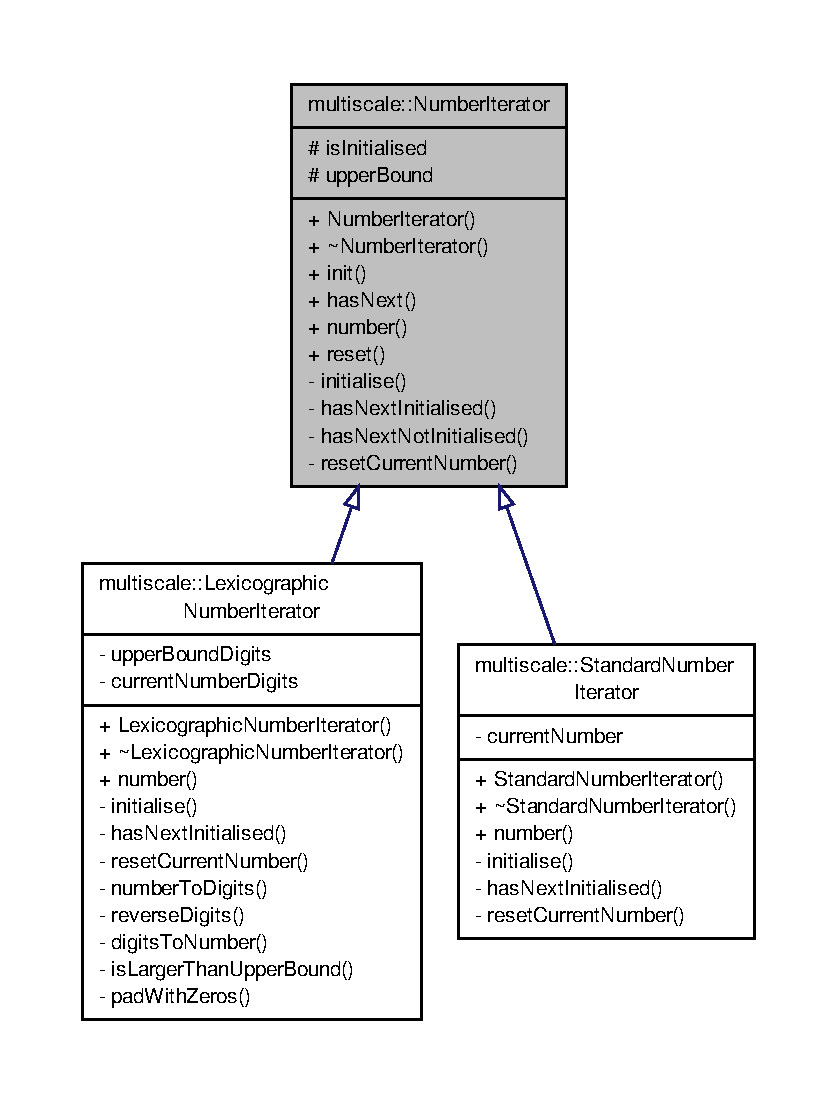
\includegraphics[width=350pt]{classmultiscale_1_1NumberIterator__inherit__graph}
\end{center}
\end{figure}


Collaboration diagram for multiscale\-:\-:Number\-Iterator\-:
\nopagebreak
\begin{figure}[H]
\begin{center}
\leavevmode
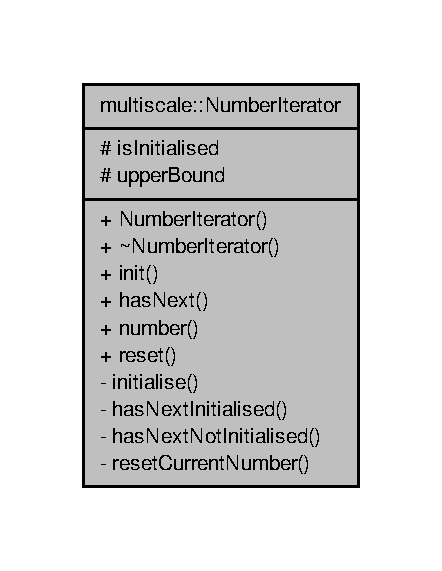
\includegraphics[width=212pt]{classmultiscale_1_1NumberIterator__coll__graph}
\end{center}
\end{figure}
\subsection*{Public Member Functions}
\begin{DoxyCompactItemize}
\item 
\hyperlink{classmultiscale_1_1NumberIterator_adc85caa104c89062cb7c3072b65da827}{Number\-Iterator} (unsigned int \hyperlink{classmultiscale_1_1NumberIterator_a56a5558958778bbde64e249d67cba886}{upper\-Bound})
\item 
virtual \hyperlink{classmultiscale_1_1NumberIterator_aae2ce809339ed853f49619ad69596229}{$\sim$\-Number\-Iterator} ()
\item 
void \hyperlink{classmultiscale_1_1NumberIterator_a7bec93b2150c52b022de484c49b551e0}{init} (unsigned int \hyperlink{classmultiscale_1_1NumberIterator_a56a5558958778bbde64e249d67cba886}{upper\-Bound})
\begin{DoxyCompactList}\small\item\em Initialise the iterator considering the given upper bound. \end{DoxyCompactList}\item 
bool \hyperlink{classmultiscale_1_1NumberIterator_a9169e7244347d2dbd657ad4f36b55f5b}{has\-Next} ()
\begin{DoxyCompactList}\small\item\em Check if there is a next number. \end{DoxyCompactList}\item 
virtual unsigned int \hyperlink{classmultiscale_1_1NumberIterator_a967fc14523f8726d5d6352d4ed6439ca}{number} ()=0
\begin{DoxyCompactList}\small\item\em Get the number pointed by the iterator. \end{DoxyCompactList}\item 
void \hyperlink{classmultiscale_1_1NumberIterator_a9e22075eb67dd5ebf4b03a4a67734a36}{reset} ()
\begin{DoxyCompactList}\small\item\em Reset the iterator. \end{DoxyCompactList}\end{DoxyCompactItemize}
\subsection*{Protected Attributes}
\begin{DoxyCompactItemize}
\item 
bool \hyperlink{classmultiscale_1_1NumberIterator_ae3d929444e14677de0b616a059380f3f}{is\-Initialised}
\item 
unsigned int \hyperlink{classmultiscale_1_1NumberIterator_a56a5558958778bbde64e249d67cba886}{upper\-Bound}
\end{DoxyCompactItemize}
\subsection*{Private Member Functions}
\begin{DoxyCompactItemize}
\item 
virtual void \hyperlink{classmultiscale_1_1NumberIterator_a0bfeef7c3f120a5ae8d49d89b4529d6e}{initialise} ()=0
\begin{DoxyCompactList}\small\item\em Initialisation of the members of the class. \end{DoxyCompactList}\item 
virtual bool \hyperlink{classmultiscale_1_1NumberIterator_a3c84ccdf0e279e67861b3cce34a26588}{has\-Next\-Initialised} ()=0
\begin{DoxyCompactList}\small\item\em Check if there is a next number when in initialised state. \end{DoxyCompactList}\item 
bool \hyperlink{classmultiscale_1_1NumberIterator_a446f1ec484d5e16092674c5de25150f1}{has\-Next\-Not\-Initialised} ()
\begin{DoxyCompactList}\small\item\em Check if there is a next number when in not initialised state. \end{DoxyCompactList}\item 
virtual void \hyperlink{classmultiscale_1_1NumberIterator_a21e658de178b6c957df5ea0482e6fbd6}{reset\-Current\-Number} ()=0
\begin{DoxyCompactList}\small\item\em Reset the current number to its initial value. \end{DoxyCompactList}\end{DoxyCompactItemize}


\subsection{Detailed Description}
Abstract class representing a number iterator. 

Definition at line 7 of file Number\-Iterator.\-hpp.



\subsection{Constructor \& Destructor Documentation}
\hypertarget{classmultiscale_1_1NumberIterator_adc85caa104c89062cb7c3072b65da827}{\index{multiscale\-::\-Number\-Iterator@{multiscale\-::\-Number\-Iterator}!Number\-Iterator@{Number\-Iterator}}
\index{Number\-Iterator@{Number\-Iterator}!multiscale::NumberIterator@{multiscale\-::\-Number\-Iterator}}
\subsubsection[{Number\-Iterator}]{\setlength{\rightskip}{0pt plus 5cm}Number\-Iterator\-::\-Number\-Iterator (
\begin{DoxyParamCaption}
\item[{unsigned int}]{upper\-Bound}
\end{DoxyParamCaption}
)}}\label{classmultiscale_1_1NumberIterator_adc85caa104c89062cb7c3072b65da827}


Definition at line 6 of file Number\-Iterator.\-cpp.



References init().



Here is the call graph for this function\-:
\nopagebreak
\begin{figure}[H]
\begin{center}
\leavevmode
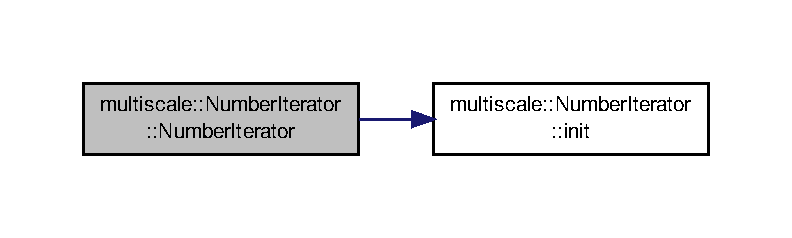
\includegraphics[width=350pt]{classmultiscale_1_1NumberIterator_adc85caa104c89062cb7c3072b65da827_cgraph}
\end{center}
\end{figure}


\hypertarget{classmultiscale_1_1NumberIterator_aae2ce809339ed853f49619ad69596229}{\index{multiscale\-::\-Number\-Iterator@{multiscale\-::\-Number\-Iterator}!$\sim$\-Number\-Iterator@{$\sim$\-Number\-Iterator}}
\index{$\sim$\-Number\-Iterator@{$\sim$\-Number\-Iterator}!multiscale::NumberIterator@{multiscale\-::\-Number\-Iterator}}
\subsubsection[{$\sim$\-Number\-Iterator}]{\setlength{\rightskip}{0pt plus 5cm}virtual multiscale\-::\-Number\-Iterator\-::$\sim$\-Number\-Iterator (
\begin{DoxyParamCaption}
{}
\end{DoxyParamCaption}
)\hspace{0.3cm}{\ttfamily [inline]}, {\ttfamily [virtual]}}}\label{classmultiscale_1_1NumberIterator_aae2ce809339ed853f49619ad69596229}


Definition at line 17 of file Number\-Iterator.\-hpp.



\subsection{Member Function Documentation}
\hypertarget{classmultiscale_1_1NumberIterator_a9169e7244347d2dbd657ad4f36b55f5b}{\index{multiscale\-::\-Number\-Iterator@{multiscale\-::\-Number\-Iterator}!has\-Next@{has\-Next}}
\index{has\-Next@{has\-Next}!multiscale::NumberIterator@{multiscale\-::\-Number\-Iterator}}
\subsubsection[{has\-Next}]{\setlength{\rightskip}{0pt plus 5cm}bool Number\-Iterator\-::has\-Next (
\begin{DoxyParamCaption}
{}
\end{DoxyParamCaption}
)}}\label{classmultiscale_1_1NumberIterator_a9169e7244347d2dbd657ad4f36b55f5b}


Check if there is a next number. 



Definition at line 14 of file Number\-Iterator.\-cpp.



References has\-Next\-Initialised(), has\-Next\-Not\-Initialised(), and is\-Initialised.



Referenced by main().



Here is the call graph for this function\-:
\nopagebreak
\begin{figure}[H]
\begin{center}
\leavevmode
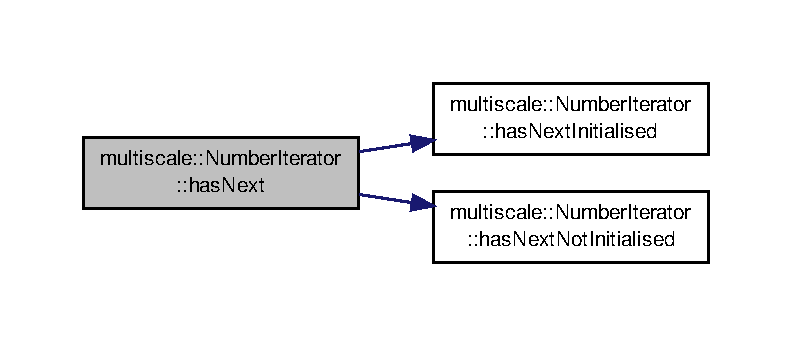
\includegraphics[width=350pt]{classmultiscale_1_1NumberIterator_a9169e7244347d2dbd657ad4f36b55f5b_cgraph}
\end{center}
\end{figure}




Here is the caller graph for this function\-:
\nopagebreak
\begin{figure}[H]
\begin{center}
\leavevmode
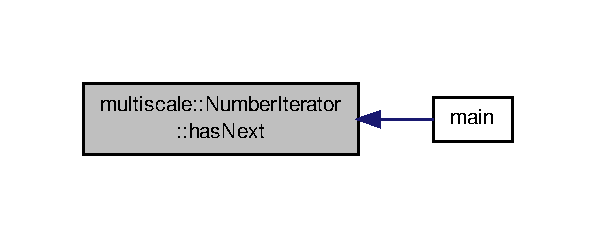
\includegraphics[width=286pt]{classmultiscale_1_1NumberIterator_a9169e7244347d2dbd657ad4f36b55f5b_icgraph}
\end{center}
\end{figure}


\hypertarget{classmultiscale_1_1NumberIterator_a3c84ccdf0e279e67861b3cce34a26588}{\index{multiscale\-::\-Number\-Iterator@{multiscale\-::\-Number\-Iterator}!has\-Next\-Initialised@{has\-Next\-Initialised}}
\index{has\-Next\-Initialised@{has\-Next\-Initialised}!multiscale::NumberIterator@{multiscale\-::\-Number\-Iterator}}
\subsubsection[{has\-Next\-Initialised}]{\setlength{\rightskip}{0pt plus 5cm}virtual bool multiscale\-::\-Number\-Iterator\-::has\-Next\-Initialised (
\begin{DoxyParamCaption}
{}
\end{DoxyParamCaption}
)\hspace{0.3cm}{\ttfamily [private]}, {\ttfamily [pure virtual]}}}\label{classmultiscale_1_1NumberIterator_a3c84ccdf0e279e67861b3cce34a26588}


Check if there is a next number when in initialised state. 



Implemented in \hyperlink{classmultiscale_1_1LexicographicNumberIterator_ac2754a1a57005183e2c9040719c97448}{multiscale\-::\-Lexicographic\-Number\-Iterator}, and \hyperlink{classmultiscale_1_1StandardNumberIterator_af840d952fae019b7e894a4a238c7d4d8}{multiscale\-::\-Standard\-Number\-Iterator}.



Referenced by has\-Next().



Here is the caller graph for this function\-:
\nopagebreak
\begin{figure}[H]
\begin{center}
\leavevmode
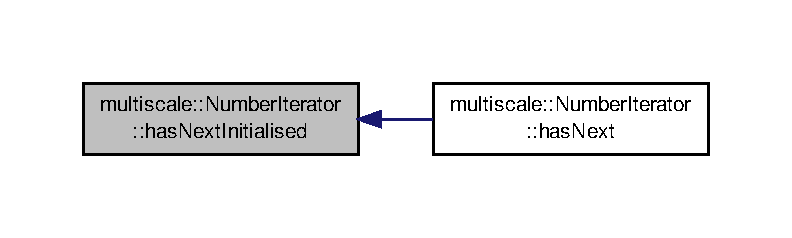
\includegraphics[width=350pt]{classmultiscale_1_1NumberIterator_a3c84ccdf0e279e67861b3cce34a26588_icgraph}
\end{center}
\end{figure}


\hypertarget{classmultiscale_1_1NumberIterator_a446f1ec484d5e16092674c5de25150f1}{\index{multiscale\-::\-Number\-Iterator@{multiscale\-::\-Number\-Iterator}!has\-Next\-Not\-Initialised@{has\-Next\-Not\-Initialised}}
\index{has\-Next\-Not\-Initialised@{has\-Next\-Not\-Initialised}!multiscale::NumberIterator@{multiscale\-::\-Number\-Iterator}}
\subsubsection[{has\-Next\-Not\-Initialised}]{\setlength{\rightskip}{0pt plus 5cm}bool Number\-Iterator\-::has\-Next\-Not\-Initialised (
\begin{DoxyParamCaption}
{}
\end{DoxyParamCaption}
)\hspace{0.3cm}{\ttfamily [private]}}}\label{classmultiscale_1_1NumberIterator_a446f1ec484d5e16092674c5de25150f1}


Check if there is a next number when in not initialised state. 



Definition at line 28 of file Number\-Iterator.\-cpp.



References is\-Initialised.



Referenced by has\-Next().



Here is the caller graph for this function\-:
\nopagebreak
\begin{figure}[H]
\begin{center}
\leavevmode
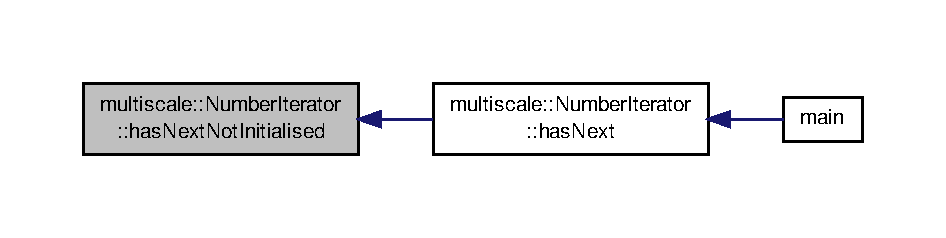
\includegraphics[width=350pt]{classmultiscale_1_1NumberIterator_a446f1ec484d5e16092674c5de25150f1_icgraph}
\end{center}
\end{figure}


\hypertarget{classmultiscale_1_1NumberIterator_a7bec93b2150c52b022de484c49b551e0}{\index{multiscale\-::\-Number\-Iterator@{multiscale\-::\-Number\-Iterator}!init@{init}}
\index{init@{init}!multiscale::NumberIterator@{multiscale\-::\-Number\-Iterator}}
\subsubsection[{init}]{\setlength{\rightskip}{0pt plus 5cm}void Number\-Iterator\-::init (
\begin{DoxyParamCaption}
\item[{unsigned int}]{upper\-Bound}
\end{DoxyParamCaption}
)}}\label{classmultiscale_1_1NumberIterator_a7bec93b2150c52b022de484c49b551e0}


Initialise the iterator considering the given upper bound. 


\begin{DoxyParams}{Parameters}
{\em upper\-Bound} & The upper bound \\
\hline
\end{DoxyParams}


Definition at line 10 of file Number\-Iterator.\-cpp.



References upper\-Bound.



Referenced by Number\-Iterator().



Here is the caller graph for this function\-:
\nopagebreak
\begin{figure}[H]
\begin{center}
\leavevmode
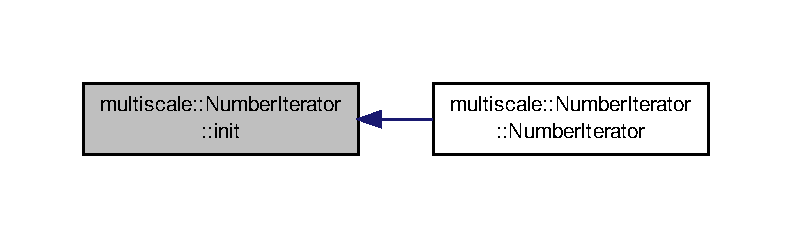
\includegraphics[width=350pt]{classmultiscale_1_1NumberIterator_a7bec93b2150c52b022de484c49b551e0_icgraph}
\end{center}
\end{figure}


\hypertarget{classmultiscale_1_1NumberIterator_a0bfeef7c3f120a5ae8d49d89b4529d6e}{\index{multiscale\-::\-Number\-Iterator@{multiscale\-::\-Number\-Iterator}!initialise@{initialise}}
\index{initialise@{initialise}!multiscale::NumberIterator@{multiscale\-::\-Number\-Iterator}}
\subsubsection[{initialise}]{\setlength{\rightskip}{0pt plus 5cm}virtual void multiscale\-::\-Number\-Iterator\-::initialise (
\begin{DoxyParamCaption}
{}
\end{DoxyParamCaption}
)\hspace{0.3cm}{\ttfamily [private]}, {\ttfamily [pure virtual]}}}\label{classmultiscale_1_1NumberIterator_a0bfeef7c3f120a5ae8d49d89b4529d6e}


Initialisation of the members of the class. 



Implemented in \hyperlink{classmultiscale_1_1LexicographicNumberIterator_a943745c4723ed8c3c18df9f92bf94d2c}{multiscale\-::\-Lexicographic\-Number\-Iterator}, and \hyperlink{classmultiscale_1_1StandardNumberIterator_a90d4512fe2d15f9bc5a78396d0092c6a}{multiscale\-::\-Standard\-Number\-Iterator}.

\hypertarget{classmultiscale_1_1NumberIterator_a967fc14523f8726d5d6352d4ed6439ca}{\index{multiscale\-::\-Number\-Iterator@{multiscale\-::\-Number\-Iterator}!number@{number}}
\index{number@{number}!multiscale::NumberIterator@{multiscale\-::\-Number\-Iterator}}
\subsubsection[{number}]{\setlength{\rightskip}{0pt plus 5cm}virtual unsigned int multiscale\-::\-Number\-Iterator\-::number (
\begin{DoxyParamCaption}
{}
\end{DoxyParamCaption}
)\hspace{0.3cm}{\ttfamily [pure virtual]}}}\label{classmultiscale_1_1NumberIterator_a967fc14523f8726d5d6352d4ed6439ca}


Get the number pointed by the iterator. 



Implemented in \hyperlink{classmultiscale_1_1LexicographicNumberIterator_a282d970d0d1a33d2736bbdf104c18336}{multiscale\-::\-Lexicographic\-Number\-Iterator}, and \hyperlink{classmultiscale_1_1StandardNumberIterator_a9071fcd0f94b3520a76ed22faed97353}{multiscale\-::\-Standard\-Number\-Iterator}.

\hypertarget{classmultiscale_1_1NumberIterator_a9e22075eb67dd5ebf4b03a4a67734a36}{\index{multiscale\-::\-Number\-Iterator@{multiscale\-::\-Number\-Iterator}!reset@{reset}}
\index{reset@{reset}!multiscale::NumberIterator@{multiscale\-::\-Number\-Iterator}}
\subsubsection[{reset}]{\setlength{\rightskip}{0pt plus 5cm}void Number\-Iterator\-::reset (
\begin{DoxyParamCaption}
{}
\end{DoxyParamCaption}
)}}\label{classmultiscale_1_1NumberIterator_a9e22075eb67dd5ebf4b03a4a67734a36}


Reset the iterator. 

Reset the iterator such that it is not initialised and the value of the current number is reset to its initial value 

Definition at line 22 of file Number\-Iterator.\-cpp.



References is\-Initialised, and reset\-Current\-Number().



Referenced by multiscale\-::\-Lexicographic\-Number\-Iterator\-::\-Lexicographic\-Number\-Iterator(), and multiscale\-::\-Standard\-Number\-Iterator\-::\-Standard\-Number\-Iterator().



Here is the call graph for this function\-:
\nopagebreak
\begin{figure}[H]
\begin{center}
\leavevmode
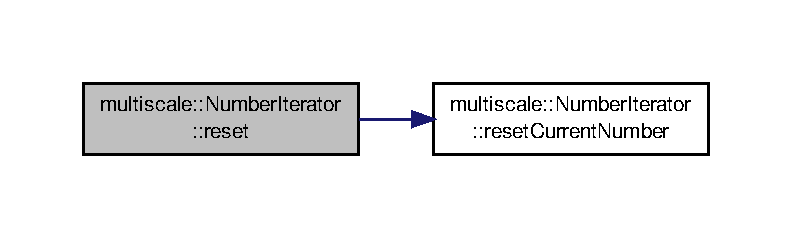
\includegraphics[width=350pt]{classmultiscale_1_1NumberIterator_a9e22075eb67dd5ebf4b03a4a67734a36_cgraph}
\end{center}
\end{figure}




Here is the caller graph for this function\-:
\nopagebreak
\begin{figure}[H]
\begin{center}
\leavevmode
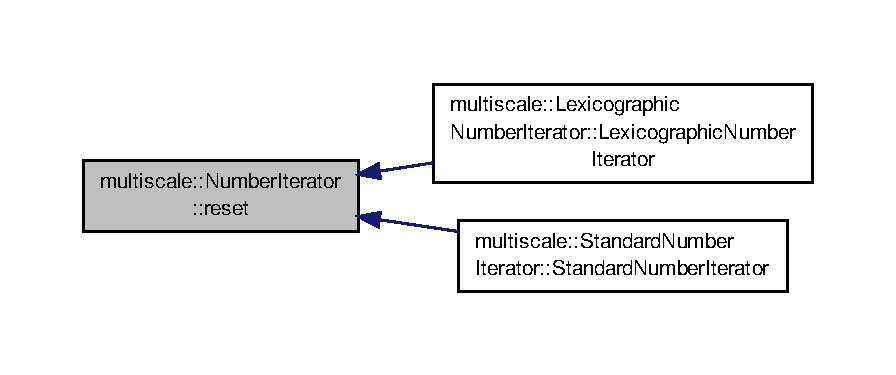
\includegraphics[width=350pt]{classmultiscale_1_1NumberIterator_a9e22075eb67dd5ebf4b03a4a67734a36_icgraph}
\end{center}
\end{figure}


\hypertarget{classmultiscale_1_1NumberIterator_a21e658de178b6c957df5ea0482e6fbd6}{\index{multiscale\-::\-Number\-Iterator@{multiscale\-::\-Number\-Iterator}!reset\-Current\-Number@{reset\-Current\-Number}}
\index{reset\-Current\-Number@{reset\-Current\-Number}!multiscale::NumberIterator@{multiscale\-::\-Number\-Iterator}}
\subsubsection[{reset\-Current\-Number}]{\setlength{\rightskip}{0pt plus 5cm}virtual void multiscale\-::\-Number\-Iterator\-::reset\-Current\-Number (
\begin{DoxyParamCaption}
{}
\end{DoxyParamCaption}
)\hspace{0.3cm}{\ttfamily [private]}, {\ttfamily [pure virtual]}}}\label{classmultiscale_1_1NumberIterator_a21e658de178b6c957df5ea0482e6fbd6}


Reset the current number to its initial value. 



Implemented in \hyperlink{classmultiscale_1_1LexicographicNumberIterator_a18311f68a49156a415c817a947abcd7d}{multiscale\-::\-Lexicographic\-Number\-Iterator}, and \hyperlink{classmultiscale_1_1StandardNumberIterator_a678d43170a27106e1d8c5475b7088d9e}{multiscale\-::\-Standard\-Number\-Iterator}.



Referenced by reset().



Here is the caller graph for this function\-:
\nopagebreak
\begin{figure}[H]
\begin{center}
\leavevmode
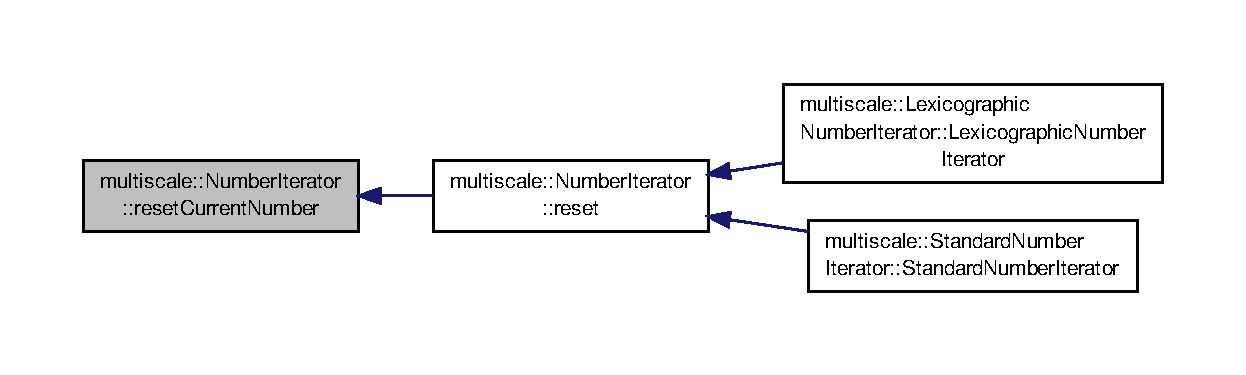
\includegraphics[width=350pt]{classmultiscale_1_1NumberIterator_a21e658de178b6c957df5ea0482e6fbd6_icgraph}
\end{center}
\end{figure}




\subsection{Member Data Documentation}
\hypertarget{classmultiscale_1_1NumberIterator_ae3d929444e14677de0b616a059380f3f}{\index{multiscale\-::\-Number\-Iterator@{multiscale\-::\-Number\-Iterator}!is\-Initialised@{is\-Initialised}}
\index{is\-Initialised@{is\-Initialised}!multiscale::NumberIterator@{multiscale\-::\-Number\-Iterator}}
\subsubsection[{is\-Initialised}]{\setlength{\rightskip}{0pt plus 5cm}bool multiscale\-::\-Number\-Iterator\-::is\-Initialised\hspace{0.3cm}{\ttfamily [protected]}}}\label{classmultiscale_1_1NumberIterator_ae3d929444e14677de0b616a059380f3f}
Flag for checking if the iterator was initialised 

Definition at line 11 of file Number\-Iterator.\-hpp.



Referenced by has\-Next(), has\-Next\-Not\-Initialised(), and reset().

\hypertarget{classmultiscale_1_1NumberIterator_a56a5558958778bbde64e249d67cba886}{\index{multiscale\-::\-Number\-Iterator@{multiscale\-::\-Number\-Iterator}!upper\-Bound@{upper\-Bound}}
\index{upper\-Bound@{upper\-Bound}!multiscale::NumberIterator@{multiscale\-::\-Number\-Iterator}}
\subsubsection[{upper\-Bound}]{\setlength{\rightskip}{0pt plus 5cm}unsigned int multiscale\-::\-Number\-Iterator\-::upper\-Bound\hspace{0.3cm}{\ttfamily [protected]}}}\label{classmultiscale_1_1NumberIterator_a56a5558958778bbde64e249d67cba886}
Upper bound of the iterator 

Definition at line 12 of file Number\-Iterator.\-hpp.



Referenced by multiscale\-::\-Standard\-Number\-Iterator\-::has\-Next\-Initialised(), init(), multiscale\-::\-Lexicographic\-Number\-Iterator\-::initialise(), and multiscale\-::\-Lexicographic\-Number\-Iterator\-::pad\-With\-Zeros().



The documentation for this class was generated from the following files\-:\begin{DoxyCompactItemize}
\item 
/home/ovidiu/\-Repositories/git/multiscale/\-Multiscale/modules/util/include/multiscale/util/\hyperlink{NumberIterator_8hpp}{Number\-Iterator.\-hpp}\item 
/home/ovidiu/\-Repositories/git/multiscale/\-Multiscale/modules/util/src/\hyperlink{NumberIterator_8cpp}{Number\-Iterator.\-cpp}\end{DoxyCompactItemize}

\hypertarget{classmultiscale_1_1NumericRangeManipulator}{\section{multiscale\-:\-:Numeric\-Range\-Manipulator Class Reference}
\label{classmultiscale_1_1NumericRangeManipulator}\index{multiscale\-::\-Numeric\-Range\-Manipulator@{multiscale\-::\-Numeric\-Range\-Manipulator}}
}


Operations for ranges of numeric values.  




{\ttfamily \#include $<$Numeric\-Range\-Manipulator.\-hpp$>$}



Collaboration diagram for multiscale\-:\-:Numeric\-Range\-Manipulator\-:
\nopagebreak
\begin{figure}[H]
\begin{center}
\leavevmode
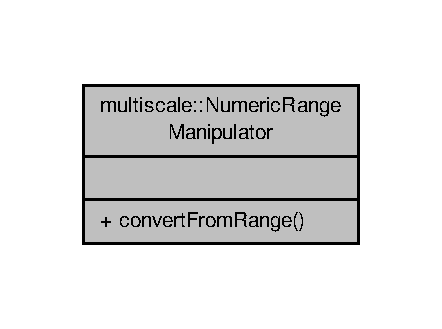
\includegraphics[width=212pt]{classmultiscale_1_1NumericRangeManipulator__coll__graph}
\end{center}
\end{figure}
\subsection*{Static Public Member Functions}
\begin{DoxyCompactItemize}
\item 
{\footnotesize template$<$class T , class U $>$ }\\static U \hyperlink{classmultiscale_1_1NumericRangeManipulator_a4459c449fb7ebc07bcb8934d3a860e7e}{convert\-From\-Range} (T old\-Range\-Min, T old\-Range\-Max, U new\-Range\-Min, U new\-Range\-Max, T old\-Value)
\begin{DoxyCompactList}\small\item\em Convert a value from an old range to a new one. \end{DoxyCompactList}\end{DoxyCompactItemize}


\subsection{Detailed Description}
Operations for ranges of numeric values. 

Definition at line 7 of file Numeric\-Range\-Manipulator.\-hpp.



\subsection{Member Function Documentation}
\hypertarget{classmultiscale_1_1NumericRangeManipulator_a4459c449fb7ebc07bcb8934d3a860e7e}{\index{multiscale\-::\-Numeric\-Range\-Manipulator@{multiscale\-::\-Numeric\-Range\-Manipulator}!convert\-From\-Range@{convert\-From\-Range}}
\index{convert\-From\-Range@{convert\-From\-Range}!multiscale::NumericRangeManipulator@{multiscale\-::\-Numeric\-Range\-Manipulator}}
\subsubsection[{convert\-From\-Range}]{\setlength{\rightskip}{0pt plus 5cm}template$<$class T , class U $>$ static U multiscale\-::\-Numeric\-Range\-Manipulator\-::convert\-From\-Range (
\begin{DoxyParamCaption}
\item[{T}]{old\-Range\-Min, }
\item[{T}]{old\-Range\-Max, }
\item[{U}]{new\-Range\-Min, }
\item[{U}]{new\-Range\-Max, }
\item[{T}]{old\-Value}
\end{DoxyParamCaption}
)\hspace{0.3cm}{\ttfamily [inline]}, {\ttfamily [static]}}}\label{classmultiscale_1_1NumericRangeManipulator_a4459c449fb7ebc07bcb8934d3a860e7e}


Convert a value from an old range to a new one. 


\begin{DoxyParams}{Parameters}
{\em old\-Range\-Min} & The minimum of the old range \\
\hline
{\em old\-Range\-Max} & The maximum of the old range \\
\hline
{\em new\-Range\-Min} & The minimum of the new range \\
\hline
{\em new\-Range\-Max} & The maximum of the new range \\
\hline
{\em old\-Value} & The old value \\
\hline
\end{DoxyParams}


Definition at line 20 of file Numeric\-Range\-Manipulator.\-hpp.



The documentation for this class was generated from the following file\-:\begin{DoxyCompactItemize}
\item 
/home/ovidiu/\-Repositories/git/multiscale/\-Multiscale/modules/util/include/multiscale/util/\hyperlink{NumericRangeManipulator_8hpp}{Numeric\-Range\-Manipulator.\-hpp}\end{DoxyCompactItemize}

\hypertarget{classmultiscale_1_1video_1_1PolarCsvToInputFilesConverter}{\section{multiscale\-:\-:video\-:\-:Polar\-Csv\-To\-Input\-Files\-Converter Class Reference}
\label{classmultiscale_1_1video_1_1PolarCsvToInputFilesConverter}\index{multiscale\-::video\-::\-Polar\-Csv\-To\-Input\-Files\-Converter@{multiscale\-::video\-::\-Polar\-Csv\-To\-Input\-Files\-Converter}}
}


Csv file to input file converter considering polar coordinates.  




{\ttfamily \#include $<$Polar\-Csv\-To\-Input\-Files\-Converter.\-hpp$>$}



Collaboration diagram for multiscale\-:\-:video\-:\-:Polar\-Csv\-To\-Input\-Files\-Converter\-:\nopagebreak
\begin{figure}[H]
\begin{center}
\leavevmode
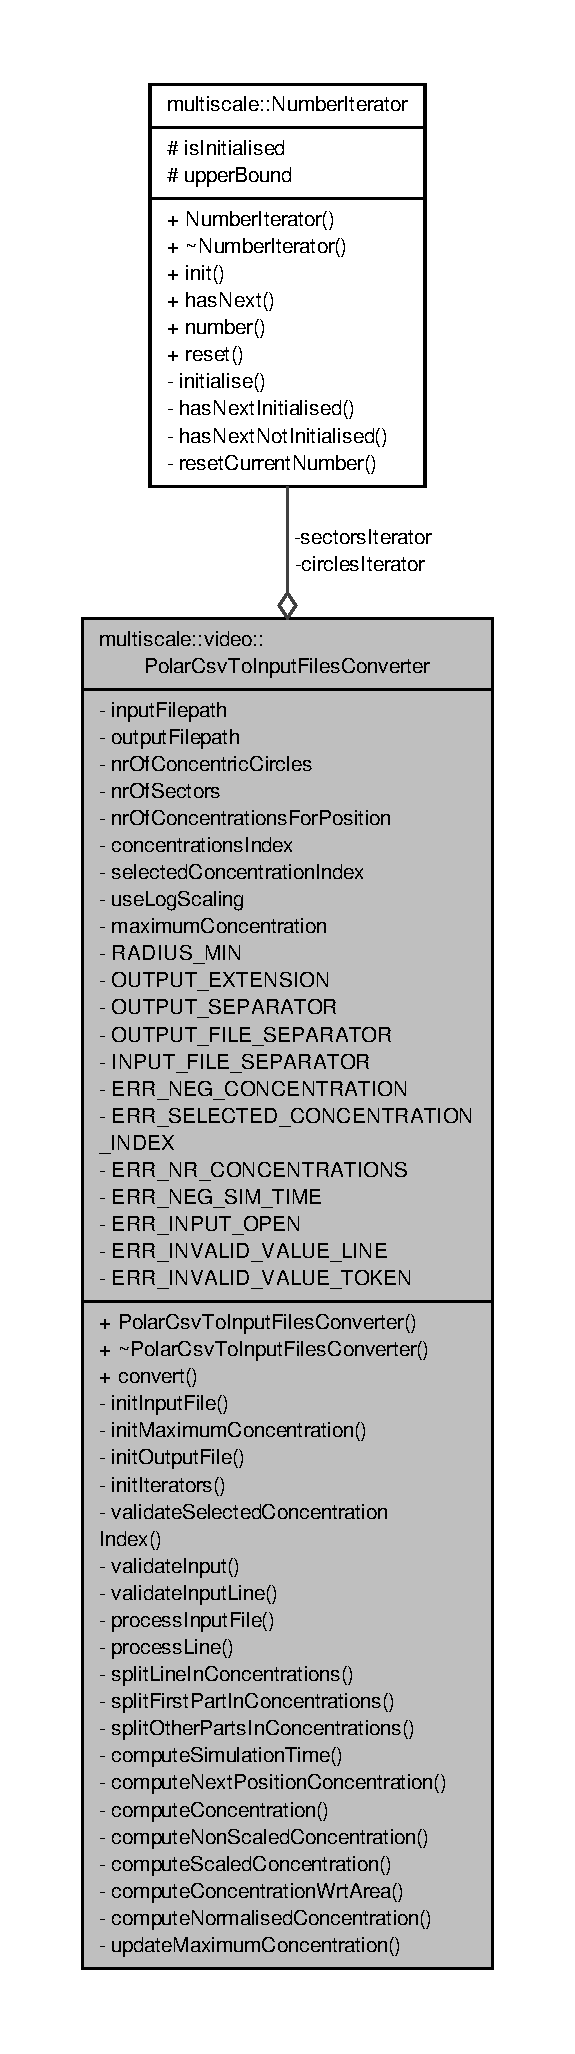
\includegraphics[height=550pt]{classmultiscale_1_1video_1_1PolarCsvToInputFilesConverter__coll__graph}
\end{center}
\end{figure}
\subsection*{Public Member Functions}
\begin{DoxyCompactItemize}
\item 
\hyperlink{classmultiscale_1_1video_1_1PolarCsvToInputFilesConverter_a4e3b77194b9706370e25b7eeba416cda}{Polar\-Csv\-To\-Input\-Files\-Converter} (const string \&\hyperlink{classmultiscale_1_1video_1_1PolarCsvToInputFilesConverter_a7b33b6d00b5e0d809f4fb0d76985ab59}{input\-Filepath}, const string \&\hyperlink{classmultiscale_1_1video_1_1PolarCsvToInputFilesConverter_a1033d31c9bfc7ccad08337c7b0fa6e6e}{output\-Filepath}, unsigned int \hyperlink{classmultiscale_1_1video_1_1PolarCsvToInputFilesConverter_a7aa37d18880e822369cbe118a093e24f}{nr\-Of\-Concentric\-Circles}, unsigned int \hyperlink{classmultiscale_1_1video_1_1PolarCsvToInputFilesConverter_a9246a2c9749602af145d5579bde8a9d1}{nr\-Of\-Sectors}, unsigned int \hyperlink{classmultiscale_1_1video_1_1PolarCsvToInputFilesConverter_a3a9301788514c50c295ca113a4114938}{nr\-Of\-Concentrations\-For\-Position}, unsigned int \hyperlink{classmultiscale_1_1video_1_1PolarCsvToInputFilesConverter_a121d592659f9f5075c8c78aa46c2950c}{selected\-Concentration\-Index}, bool \hyperlink{classmultiscale_1_1video_1_1PolarCsvToInputFilesConverter_af07bf56fc39bb226a6e2596f35ada0d7}{use\-Log\-Scaling}, \hyperlink{namespacemultiscale_a6ef911f4d48a4bf5e657c237ec169ff5}{Number\-Iterator\-Type} number\-Iterator\-Type)
\item 
\hyperlink{classmultiscale_1_1video_1_1PolarCsvToInputFilesConverter_afdd156ae24d5d6194b113dd661110ed5}{$\sim$\-Polar\-Csv\-To\-Input\-Files\-Converter} ()
\item 
void \hyperlink{classmultiscale_1_1video_1_1PolarCsvToInputFilesConverter_a818c188569ad54cb0cfbbaa2bd32356c}{convert} ()
\begin{DoxyCompactList}\small\item\em Start the conversion. \end{DoxyCompactList}\end{DoxyCompactItemize}
\subsection*{Private Member Functions}
\begin{DoxyCompactItemize}
\item 
void \hyperlink{classmultiscale_1_1video_1_1PolarCsvToInputFilesConverter_a8157549bbbcf7951e26c7af96ffe4a4b}{init\-Input\-File} (ifstream \&fin)
\begin{DoxyCompactList}\small\item\em Initialise the input file stream over the given input file. \end{DoxyCompactList}\item 
void \hyperlink{classmultiscale_1_1video_1_1PolarCsvToInputFilesConverter_a987936fd605863f1d51d29d315b5f842}{init\-Maximum\-Concentration} (ifstream \&fin)
\begin{DoxyCompactList}\small\item\em Compute the value of member maximum concentration. \end{DoxyCompactList}\item 
void \hyperlink{classmultiscale_1_1video_1_1PolarCsvToInputFilesConverter_a03d74df6e7a0b18c5099eb39f3e4fc7c}{init\-Output\-File} (ofstream \&fout, unsigned int index, double \&simulation\-Time)
\begin{DoxyCompactList}\small\item\em Initialise the output file with the given index and simulation time. \end{DoxyCompactList}\item 
void \hyperlink{classmultiscale_1_1video_1_1PolarCsvToInputFilesConverter_aba034b15162728c82b56b85b9074162c}{init\-Iterators} (const \hyperlink{namespacemultiscale_a6ef911f4d48a4bf5e657c237ec169ff5}{Number\-Iterator\-Type} \&number\-Iterator\-Type)
\begin{DoxyCompactList}\small\item\em Initialise the iterators considering the given number iterator type. \end{DoxyCompactList}\item 
void \hyperlink{classmultiscale_1_1video_1_1PolarCsvToInputFilesConverter_a95a32c02de43f1837f3592e4b9f03b48}{validate\-Selected\-Concentration\-Index} ()
\begin{DoxyCompactList}\small\item\em Validate the selected concentration index in case of more than one concentration for each position. \end{DoxyCompactList}\item 
void \hyperlink{classmultiscale_1_1video_1_1PolarCsvToInputFilesConverter_af612ef958fd3656f2c477d4d8e81244a}{validate\-Input} (ifstream \&fin)
\begin{DoxyCompactList}\small\item\em Validate the input. \end{DoxyCompactList}\item 
void \hyperlink{classmultiscale_1_1video_1_1PolarCsvToInputFilesConverter_a71741de958cfecc133a303ea3a5af22c}{validate\-Input\-Line} (const string \&line, unsigned int line\-Number)
\begin{DoxyCompactList}\small\item\em Validate the provided line identified by a line number. \end{DoxyCompactList}\item 
void \hyperlink{classmultiscale_1_1video_1_1PolarCsvToInputFilesConverter_a66168d7550e656dccf01a473ed2708f0}{process\-Input\-File} (ifstream \&fin)
\begin{DoxyCompactList}\small\item\em Process the input file. \end{DoxyCompactList}\item 
void \hyperlink{classmultiscale_1_1video_1_1PolarCsvToInputFilesConverter_a23c483d80d7c0c8f0510595a1ab55f69}{process\-Line} (const string \&line, unsigned int output\-Index)
\begin{DoxyCompactList}\small\item\em Process the provided line. \end{DoxyCompactList}\item 
vector$<$ double $>$ \hyperlink{classmultiscale_1_1video_1_1PolarCsvToInputFilesConverter_af2d31d32cdba42aeb5589b3faab315ad}{split\-Line\-In\-Concentrations} (const string \&line, double \&simulation\-Time)
\begin{DoxyCompactList}\small\item\em Split the line in concentrations. \end{DoxyCompactList}\item 
void \hyperlink{classmultiscale_1_1video_1_1PolarCsvToInputFilesConverter_a2ab8a181fa30c720d4ee87c188770bcc}{split\-First\-Part\-In\-Concentrations} (vector$<$ double $>$ \&concentrations, const vector$<$ string $>$ \&tokens, unsigned int circle\-Index)
\begin{DoxyCompactList}\small\item\em Split first part of the line (i.\-e. part representing the origin) into concentrations. \end{DoxyCompactList}\item 
void \hyperlink{classmultiscale_1_1video_1_1PolarCsvToInputFilesConverter_a84994d623303296509326707fa397f29}{split\-Other\-Parts\-In\-Concentrations} (vector$<$ double $>$ \&concentrations, const vector$<$ string $>$ \&tokens, unsigned int circle\-Index)
\begin{DoxyCompactList}\small\item\em Split other parts of the line (i.\-e. non-\/first part) into concentrations. \end{DoxyCompactList}\item 
double \hyperlink{classmultiscale_1_1video_1_1PolarCsvToInputFilesConverter_a3f811086d08d1665548af54e8bd50654}{compute\-Simulation\-Time} (const string \&token)
\begin{DoxyCompactList}\small\item\em Compute the simulation time from the given token and check if it is valid. \end{DoxyCompactList}\item 
double \hyperlink{classmultiscale_1_1video_1_1PolarCsvToInputFilesConverter_a393e66a46463bf557ccf318ddcf14d3a}{compute\-Next\-Position\-Concentration} (unsigned int circle\-Index, int concentration\-Index, const vector$<$ string $>$ \&tokens)
\begin{DoxyCompactList}\small\item\em Compute the concentration for the next position. \end{DoxyCompactList}\item 
double \hyperlink{classmultiscale_1_1video_1_1PolarCsvToInputFilesConverter_adec57e72f9f321cd9b36317b2aa3ac38}{compute\-Concentration} (const string \&concentration, int circle\-Index)
\begin{DoxyCompactList}\small\item\em Compute the concentration from the given string considering the index of the current concentric circle. \end{DoxyCompactList}\item 
double \hyperlink{classmultiscale_1_1video_1_1PolarCsvToInputFilesConverter_a3c9fd506cbe4d0881ed3c234492d2432}{compute\-Non\-Scaled\-Concentration} (const string \&concentration, int circle\-Index)
\begin{DoxyCompactList}\small\item\em Compute the non-\/scaled concentration from the given string considering the index of the current concentric circle. \end{DoxyCompactList}\item 
double \hyperlink{classmultiscale_1_1video_1_1PolarCsvToInputFilesConverter_adfaf1d1912fa6f511033ace081381ac8}{compute\-Scaled\-Concentration} (const string \&concentration, int circle\-Index)
\begin{DoxyCompactList}\small\item\em Compute the scaled concentration from the given string considering the index of the current concentric circle. \end{DoxyCompactList}\item 
double \hyperlink{classmultiscale_1_1video_1_1PolarCsvToInputFilesConverter_aa35b7d511b76a3c145e25886e2e76daa}{compute\-Concentration\-Wrt\-Area} (double amount, int circle\-Index)
\begin{DoxyCompactList}\small\item\em Compute the concentration wrt. the area of the annular sector. \end{DoxyCompactList}\item 
double \hyperlink{classmultiscale_1_1video_1_1PolarCsvToInputFilesConverter_a5fc03b210507a363037a694fdbc95b2b}{compute\-Normalised\-Concentration} (double concentration, int circle\-Index)
\begin{DoxyCompactList}\small\item\em Normalise the concentration considering the index of the current concentric circle by dividing it to the maximum concentration. \end{DoxyCompactList}\item 
void \hyperlink{classmultiscale_1_1video_1_1PolarCsvToInputFilesConverter_ae624c0a8fe97d266cbc127d64af707de}{update\-Maximum\-Concentration} (const string \&line, double \&\hyperlink{classmultiscale_1_1video_1_1PolarCsvToInputFilesConverter_a89b7dce2825cd5c8c45a1e6f19770e5f}{maximum\-Concentration})
\begin{DoxyCompactList}\small\item\em Update the maximum concentration if the values from the given line are greater than it. \end{DoxyCompactList}\end{DoxyCompactItemize}
\subsection*{Private Attributes}
\begin{DoxyCompactItemize}
\item 
string \hyperlink{classmultiscale_1_1video_1_1PolarCsvToInputFilesConverter_a7b33b6d00b5e0d809f4fb0d76985ab59}{input\-Filepath}
\item 
string \hyperlink{classmultiscale_1_1video_1_1PolarCsvToInputFilesConverter_a1033d31c9bfc7ccad08337c7b0fa6e6e}{output\-Filepath}
\item 
unsigned int \hyperlink{classmultiscale_1_1video_1_1PolarCsvToInputFilesConverter_a7aa37d18880e822369cbe118a093e24f}{nr\-Of\-Concentric\-Circles}
\item 
unsigned int \hyperlink{classmultiscale_1_1video_1_1PolarCsvToInputFilesConverter_a9246a2c9749602af145d5579bde8a9d1}{nr\-Of\-Sectors}
\item 
unsigned int \hyperlink{classmultiscale_1_1video_1_1PolarCsvToInputFilesConverter_a3a9301788514c50c295ca113a4114938}{nr\-Of\-Concentrations\-For\-Position}
\item 
unsigned int \hyperlink{classmultiscale_1_1video_1_1PolarCsvToInputFilesConverter_afd9f17e6ba2dc46b920ab28538278362}{concentrations\-Index}
\item 
unsigned int \hyperlink{classmultiscale_1_1video_1_1PolarCsvToInputFilesConverter_a121d592659f9f5075c8c78aa46c2950c}{selected\-Concentration\-Index}
\item 
bool \hyperlink{classmultiscale_1_1video_1_1PolarCsvToInputFilesConverter_af07bf56fc39bb226a6e2596f35ada0d7}{use\-Log\-Scaling}
\item 
double \hyperlink{classmultiscale_1_1video_1_1PolarCsvToInputFilesConverter_a89b7dce2825cd5c8c45a1e6f19770e5f}{maximum\-Concentration}
\item 
\hyperlink{classmultiscale_1_1NumberIterator}{Number\-Iterator} $\ast$ \hyperlink{classmultiscale_1_1video_1_1PolarCsvToInputFilesConverter_ad4cf12c7f3951f0bb388939797cbcc0c}{circles\-Iterator}
\item 
\hyperlink{classmultiscale_1_1NumberIterator}{Number\-Iterator} $\ast$ \hyperlink{classmultiscale_1_1video_1_1PolarCsvToInputFilesConverter_aa6895c1613a551cd05195f05ae51862b}{sectors\-Iterator}
\end{DoxyCompactItemize}


\subsection{Detailed Description}
Csv file to input file converter considering polar coordinates. 

Definition at line 33 of file Polar\-Csv\-To\-Input\-Files\-Converter.\-hpp.



\subsection{Constructor \& Destructor Documentation}
\hypertarget{classmultiscale_1_1video_1_1PolarCsvToInputFilesConverter_a4e3b77194b9706370e25b7eeba416cda}{\index{multiscale\-::video\-::\-Polar\-Csv\-To\-Input\-Files\-Converter@{multiscale\-::video\-::\-Polar\-Csv\-To\-Input\-Files\-Converter}!Polar\-Csv\-To\-Input\-Files\-Converter@{Polar\-Csv\-To\-Input\-Files\-Converter}}
\index{Polar\-Csv\-To\-Input\-Files\-Converter@{Polar\-Csv\-To\-Input\-Files\-Converter}!multiscale::video::PolarCsvToInputFilesConverter@{multiscale\-::video\-::\-Polar\-Csv\-To\-Input\-Files\-Converter}}
\subsubsection[{Polar\-Csv\-To\-Input\-Files\-Converter}]{\setlength{\rightskip}{0pt plus 5cm}Polar\-Csv\-To\-Input\-Files\-Converter\-::\-Polar\-Csv\-To\-Input\-Files\-Converter (
\begin{DoxyParamCaption}
\item[{const string \&}]{input\-Filepath, }
\item[{const string \&}]{output\-Filepath, }
\item[{unsigned int}]{nr\-Of\-Concentric\-Circles, }
\item[{unsigned int}]{nr\-Of\-Sectors, }
\item[{unsigned int}]{nr\-Of\-Concentrations\-For\-Position, }
\item[{unsigned int}]{selected\-Concentration\-Index, }
\item[{bool}]{use\-Log\-Scaling, }
\item[{{\bf Number\-Iterator\-Type}}]{number\-Iterator\-Type}
\end{DoxyParamCaption}
)}}\label{classmultiscale_1_1video_1_1PolarCsvToInputFilesConverter_a4e3b77194b9706370e25b7eeba416cda}


Definition at line 20 of file Polar\-Csv\-To\-Input\-Files\-Converter.\-cpp.

\hypertarget{classmultiscale_1_1video_1_1PolarCsvToInputFilesConverter_afdd156ae24d5d6194b113dd661110ed5}{\index{multiscale\-::video\-::\-Polar\-Csv\-To\-Input\-Files\-Converter@{multiscale\-::video\-::\-Polar\-Csv\-To\-Input\-Files\-Converter}!$\sim$\-Polar\-Csv\-To\-Input\-Files\-Converter@{$\sim$\-Polar\-Csv\-To\-Input\-Files\-Converter}}
\index{$\sim$\-Polar\-Csv\-To\-Input\-Files\-Converter@{$\sim$\-Polar\-Csv\-To\-Input\-Files\-Converter}!multiscale::video::PolarCsvToInputFilesConverter@{multiscale\-::video\-::\-Polar\-Csv\-To\-Input\-Files\-Converter}}
\subsubsection[{$\sim$\-Polar\-Csv\-To\-Input\-Files\-Converter}]{\setlength{\rightskip}{0pt plus 5cm}Polar\-Csv\-To\-Input\-Files\-Converter\-::$\sim$\-Polar\-Csv\-To\-Input\-Files\-Converter (
\begin{DoxyParamCaption}
{}
\end{DoxyParamCaption}
)}}\label{classmultiscale_1_1video_1_1PolarCsvToInputFilesConverter_afdd156ae24d5d6194b113dd661110ed5}


Definition at line 44 of file Polar\-Csv\-To\-Input\-Files\-Converter.\-cpp.



\subsection{Member Function Documentation}
\hypertarget{classmultiscale_1_1video_1_1PolarCsvToInputFilesConverter_adec57e72f9f321cd9b36317b2aa3ac38}{\index{multiscale\-::video\-::\-Polar\-Csv\-To\-Input\-Files\-Converter@{multiscale\-::video\-::\-Polar\-Csv\-To\-Input\-Files\-Converter}!compute\-Concentration@{compute\-Concentration}}
\index{compute\-Concentration@{compute\-Concentration}!multiscale::video::PolarCsvToInputFilesConverter@{multiscale\-::video\-::\-Polar\-Csv\-To\-Input\-Files\-Converter}}
\subsubsection[{compute\-Concentration}]{\setlength{\rightskip}{0pt plus 5cm}double Polar\-Csv\-To\-Input\-Files\-Converter\-::compute\-Concentration (
\begin{DoxyParamCaption}
\item[{const string \&}]{concentration, }
\item[{int}]{circle\-Index}
\end{DoxyParamCaption}
)\hspace{0.3cm}{\ttfamily [inline]}, {\ttfamily [private]}}}\label{classmultiscale_1_1video_1_1PolarCsvToInputFilesConverter_adec57e72f9f321cd9b36317b2aa3ac38}


Compute the concentration from the given string considering the index of the current concentric circle. 


\begin{DoxyParams}{Parameters}
{\em concentration} & String representing the concentration \\
\hline
{\em circle\-Index} & Index of the concentric circle \\
\hline
\end{DoxyParams}


Definition at line 306 of file Polar\-Csv\-To\-Input\-Files\-Converter.\-cpp.

\hypertarget{classmultiscale_1_1video_1_1PolarCsvToInputFilesConverter_aa35b7d511b76a3c145e25886e2e76daa}{\index{multiscale\-::video\-::\-Polar\-Csv\-To\-Input\-Files\-Converter@{multiscale\-::video\-::\-Polar\-Csv\-To\-Input\-Files\-Converter}!compute\-Concentration\-Wrt\-Area@{compute\-Concentration\-Wrt\-Area}}
\index{compute\-Concentration\-Wrt\-Area@{compute\-Concentration\-Wrt\-Area}!multiscale::video::PolarCsvToInputFilesConverter@{multiscale\-::video\-::\-Polar\-Csv\-To\-Input\-Files\-Converter}}
\subsubsection[{compute\-Concentration\-Wrt\-Area}]{\setlength{\rightskip}{0pt plus 5cm}double Polar\-Csv\-To\-Input\-Files\-Converter\-::compute\-Concentration\-Wrt\-Area (
\begin{DoxyParamCaption}
\item[{double}]{amount, }
\item[{int}]{circle\-Index}
\end{DoxyParamCaption}
)\hspace{0.3cm}{\ttfamily [inline]}, {\ttfamily [private]}}}\label{classmultiscale_1_1video_1_1PolarCsvToInputFilesConverter_aa35b7d511b76a3c145e25886e2e76daa}


Compute the concentration wrt. the area of the annular sector. 


\begin{DoxyParams}{Parameters}
{\em amount} & Amount in annular sector \\
\hline
{\em circle\-Index} & Index of the concentric circle which will be used to determine the area \\
\hline
\end{DoxyParams}


Definition at line 332 of file Polar\-Csv\-To\-Input\-Files\-Converter.\-cpp.

\hypertarget{classmultiscale_1_1video_1_1PolarCsvToInputFilesConverter_a393e66a46463bf557ccf318ddcf14d3a}{\index{multiscale\-::video\-::\-Polar\-Csv\-To\-Input\-Files\-Converter@{multiscale\-::video\-::\-Polar\-Csv\-To\-Input\-Files\-Converter}!compute\-Next\-Position\-Concentration@{compute\-Next\-Position\-Concentration}}
\index{compute\-Next\-Position\-Concentration@{compute\-Next\-Position\-Concentration}!multiscale::video::PolarCsvToInputFilesConverter@{multiscale\-::video\-::\-Polar\-Csv\-To\-Input\-Files\-Converter}}
\subsubsection[{compute\-Next\-Position\-Concentration}]{\setlength{\rightskip}{0pt plus 5cm}double Polar\-Csv\-To\-Input\-Files\-Converter\-::compute\-Next\-Position\-Concentration (
\begin{DoxyParamCaption}
\item[{unsigned int}]{circle\-Index, }
\item[{int}]{concentration\-Index, }
\item[{const vector$<$ string $>$ \&}]{tokens}
\end{DoxyParamCaption}
)\hspace{0.3cm}{\ttfamily [inline]}, {\ttfamily [private]}}}\label{classmultiscale_1_1video_1_1PolarCsvToInputFilesConverter_a393e66a46463bf557ccf318ddcf14d3a}


Compute the concentration for the next position. 


\begin{DoxyParams}{Parameters}
{\em circle\-Index} & Index of the current concentric circle \\
\hline
{\em concentration\-Index} & Index of the current concentration from the vector of tokens \\
\hline
{\em tokens} & Vector of tokens \\
\hline
\end{DoxyParams}


Definition at line 277 of file Polar\-Csv\-To\-Input\-Files\-Converter.\-cpp.

\hypertarget{classmultiscale_1_1video_1_1PolarCsvToInputFilesConverter_a3c9fd506cbe4d0881ed3c234492d2432}{\index{multiscale\-::video\-::\-Polar\-Csv\-To\-Input\-Files\-Converter@{multiscale\-::video\-::\-Polar\-Csv\-To\-Input\-Files\-Converter}!compute\-Non\-Scaled\-Concentration@{compute\-Non\-Scaled\-Concentration}}
\index{compute\-Non\-Scaled\-Concentration@{compute\-Non\-Scaled\-Concentration}!multiscale::video::PolarCsvToInputFilesConverter@{multiscale\-::video\-::\-Polar\-Csv\-To\-Input\-Files\-Converter}}
\subsubsection[{compute\-Non\-Scaled\-Concentration}]{\setlength{\rightskip}{0pt plus 5cm}double Polar\-Csv\-To\-Input\-Files\-Converter\-::compute\-Non\-Scaled\-Concentration (
\begin{DoxyParamCaption}
\item[{const string \&}]{concentration, }
\item[{int}]{circle\-Index}
\end{DoxyParamCaption}
)\hspace{0.3cm}{\ttfamily [inline]}, {\ttfamily [private]}}}\label{classmultiscale_1_1video_1_1PolarCsvToInputFilesConverter_a3c9fd506cbe4d0881ed3c234492d2432}


Compute the non-\/scaled concentration from the given string considering the index of the current concentric circle. 


\begin{DoxyParams}{Parameters}
{\em concentration} & String representing the concentration \\
\hline
{\em circle\-Index} & Index of the concentric circle \\
\hline
\end{DoxyParams}


Definition at line 312 of file Polar\-Csv\-To\-Input\-Files\-Converter.\-cpp.

\hypertarget{classmultiscale_1_1video_1_1PolarCsvToInputFilesConverter_a5fc03b210507a363037a694fdbc95b2b}{\index{multiscale\-::video\-::\-Polar\-Csv\-To\-Input\-Files\-Converter@{multiscale\-::video\-::\-Polar\-Csv\-To\-Input\-Files\-Converter}!compute\-Normalised\-Concentration@{compute\-Normalised\-Concentration}}
\index{compute\-Normalised\-Concentration@{compute\-Normalised\-Concentration}!multiscale::video::PolarCsvToInputFilesConverter@{multiscale\-::video\-::\-Polar\-Csv\-To\-Input\-Files\-Converter}}
\subsubsection[{compute\-Normalised\-Concentration}]{\setlength{\rightskip}{0pt plus 5cm}double Polar\-Csv\-To\-Input\-Files\-Converter\-::compute\-Normalised\-Concentration (
\begin{DoxyParamCaption}
\item[{double}]{concentration, }
\item[{int}]{circle\-Index}
\end{DoxyParamCaption}
)\hspace{0.3cm}{\ttfamily [inline]}, {\ttfamily [private]}}}\label{classmultiscale_1_1video_1_1PolarCsvToInputFilesConverter_a5fc03b210507a363037a694fdbc95b2b}


Normalise the concentration considering the index of the current concentric circle by dividing it to the maximum concentration. 


\begin{DoxyParams}{Parameters}
{\em concentration} & The concentration \\
\hline
{\em circle\-Index} & Index of the concentric circle \\
\hline
\end{DoxyParams}


Definition at line 336 of file Polar\-Csv\-To\-Input\-Files\-Converter.\-cpp.

\hypertarget{classmultiscale_1_1video_1_1PolarCsvToInputFilesConverter_adfaf1d1912fa6f511033ace081381ac8}{\index{multiscale\-::video\-::\-Polar\-Csv\-To\-Input\-Files\-Converter@{multiscale\-::video\-::\-Polar\-Csv\-To\-Input\-Files\-Converter}!compute\-Scaled\-Concentration@{compute\-Scaled\-Concentration}}
\index{compute\-Scaled\-Concentration@{compute\-Scaled\-Concentration}!multiscale::video::PolarCsvToInputFilesConverter@{multiscale\-::video\-::\-Polar\-Csv\-To\-Input\-Files\-Converter}}
\subsubsection[{compute\-Scaled\-Concentration}]{\setlength{\rightskip}{0pt plus 5cm}double Polar\-Csv\-To\-Input\-Files\-Converter\-::compute\-Scaled\-Concentration (
\begin{DoxyParamCaption}
\item[{const string \&}]{concentration, }
\item[{int}]{circle\-Index}
\end{DoxyParamCaption}
)\hspace{0.3cm}{\ttfamily [inline]}, {\ttfamily [private]}}}\label{classmultiscale_1_1video_1_1PolarCsvToInputFilesConverter_adfaf1d1912fa6f511033ace081381ac8}


Compute the scaled concentration from the given string considering the index of the current concentric circle. 

Compute the scaled concentration from the given string by applying a logit transformation to it


\begin{DoxyParams}{Parameters}
{\em concentration} & String representing the concentration \\
\hline
{\em circle\-Index} & Index of the concentric circle \\
\hline
\end{DoxyParams}


Definition at line 318 of file Polar\-Csv\-To\-Input\-Files\-Converter.\-cpp.

\hypertarget{classmultiscale_1_1video_1_1PolarCsvToInputFilesConverter_a3f811086d08d1665548af54e8bd50654}{\index{multiscale\-::video\-::\-Polar\-Csv\-To\-Input\-Files\-Converter@{multiscale\-::video\-::\-Polar\-Csv\-To\-Input\-Files\-Converter}!compute\-Simulation\-Time@{compute\-Simulation\-Time}}
\index{compute\-Simulation\-Time@{compute\-Simulation\-Time}!multiscale::video::PolarCsvToInputFilesConverter@{multiscale\-::video\-::\-Polar\-Csv\-To\-Input\-Files\-Converter}}
\subsubsection[{compute\-Simulation\-Time}]{\setlength{\rightskip}{0pt plus 5cm}double Polar\-Csv\-To\-Input\-Files\-Converter\-::compute\-Simulation\-Time (
\begin{DoxyParamCaption}
\item[{const string \&}]{token}
\end{DoxyParamCaption}
)\hspace{0.3cm}{\ttfamily [inline]}, {\ttfamily [private]}}}\label{classmultiscale_1_1video_1_1PolarCsvToInputFilesConverter_a3f811086d08d1665548af54e8bd50654}


Compute the simulation time from the given token and check if it is valid. 


\begin{DoxyParams}{Parameters}
{\em token} & Token (string) \\
\hline
\end{DoxyParams}


Definition at line 267 of file Polar\-Csv\-To\-Input\-Files\-Converter.\-cpp.



References E\-R\-R\-\_\-\-N\-E\-G\-\_\-\-S\-I\-M\-\_\-\-T\-I\-M\-E.

\hypertarget{classmultiscale_1_1video_1_1PolarCsvToInputFilesConverter_a818c188569ad54cb0cfbbaa2bd32356c}{\index{multiscale\-::video\-::\-Polar\-Csv\-To\-Input\-Files\-Converter@{multiscale\-::video\-::\-Polar\-Csv\-To\-Input\-Files\-Converter}!convert@{convert}}
\index{convert@{convert}!multiscale::video::PolarCsvToInputFilesConverter@{multiscale\-::video\-::\-Polar\-Csv\-To\-Input\-Files\-Converter}}
\subsubsection[{convert}]{\setlength{\rightskip}{0pt plus 5cm}void Polar\-Csv\-To\-Input\-Files\-Converter\-::convert (
\begin{DoxyParamCaption}
{}
\end{DoxyParamCaption}
)}}\label{classmultiscale_1_1video_1_1PolarCsvToInputFilesConverter_a818c188569ad54cb0cfbbaa2bd32356c}


Start the conversion. 



Definition at line 49 of file Polar\-Csv\-To\-Input\-Files\-Converter.\-cpp.



Referenced by main().



Here is the caller graph for this function\-:\nopagebreak
\begin{figure}[H]
\begin{center}
\leavevmode
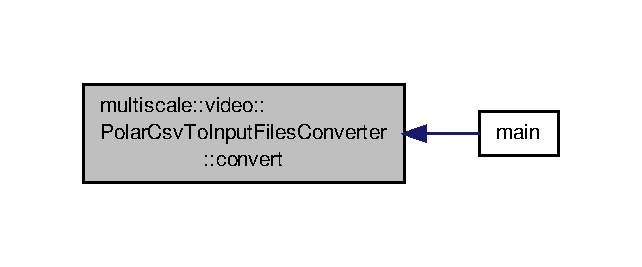
\includegraphics[width=308pt]{classmultiscale_1_1video_1_1PolarCsvToInputFilesConverter_a818c188569ad54cb0cfbbaa2bd32356c_icgraph}
\end{center}
\end{figure}


\hypertarget{classmultiscale_1_1video_1_1PolarCsvToInputFilesConverter_a8157549bbbcf7951e26c7af96ffe4a4b}{\index{multiscale\-::video\-::\-Polar\-Csv\-To\-Input\-Files\-Converter@{multiscale\-::video\-::\-Polar\-Csv\-To\-Input\-Files\-Converter}!init\-Input\-File@{init\-Input\-File}}
\index{init\-Input\-File@{init\-Input\-File}!multiscale::video::PolarCsvToInputFilesConverter@{multiscale\-::video\-::\-Polar\-Csv\-To\-Input\-Files\-Converter}}
\subsubsection[{init\-Input\-File}]{\setlength{\rightskip}{0pt plus 5cm}void Polar\-Csv\-To\-Input\-Files\-Converter\-::init\-Input\-File (
\begin{DoxyParamCaption}
\item[{ifstream \&}]{fin}
\end{DoxyParamCaption}
)\hspace{0.3cm}{\ttfamily [private]}}}\label{classmultiscale_1_1video_1_1PolarCsvToInputFilesConverter_a8157549bbbcf7951e26c7af96ffe4a4b}


Initialise the input file stream over the given input file. 


\begin{DoxyParams}{Parameters}
{\em fin} & Input file stream \\
\hline
\end{DoxyParams}


Definition at line 62 of file Polar\-Csv\-To\-Input\-Files\-Converter.\-cpp.



References E\-R\-R\-\_\-\-I\-N\-P\-U\-T\-\_\-\-O\-P\-E\-N.

\hypertarget{classmultiscale_1_1video_1_1PolarCsvToInputFilesConverter_aba034b15162728c82b56b85b9074162c}{\index{multiscale\-::video\-::\-Polar\-Csv\-To\-Input\-Files\-Converter@{multiscale\-::video\-::\-Polar\-Csv\-To\-Input\-Files\-Converter}!init\-Iterators@{init\-Iterators}}
\index{init\-Iterators@{init\-Iterators}!multiscale::video::PolarCsvToInputFilesConverter@{multiscale\-::video\-::\-Polar\-Csv\-To\-Input\-Files\-Converter}}
\subsubsection[{init\-Iterators}]{\setlength{\rightskip}{0pt plus 5cm}void Polar\-Csv\-To\-Input\-Files\-Converter\-::init\-Iterators (
\begin{DoxyParamCaption}
\item[{const {\bf Number\-Iterator\-Type} \&}]{number\-Iterator\-Type}
\end{DoxyParamCaption}
)\hspace{0.3cm}{\ttfamily [private]}}}\label{classmultiscale_1_1video_1_1PolarCsvToInputFilesConverter_aba034b15162728c82b56b85b9074162c}


Initialise the iterators considering the given number iterator type. 


\begin{DoxyParams}{Parameters}
{\em number\-Iterator\-Type} & The type of the number iterator \\
\hline
\end{DoxyParams}


Definition at line 111 of file Polar\-Csv\-To\-Input\-Files\-Converter.\-cpp.



References multiscale\-::\-L\-E\-X\-I\-C\-O\-G\-R\-A\-P\-H\-I\-C, and multiscale\-::\-S\-T\-A\-N\-D\-A\-R\-D.

\hypertarget{classmultiscale_1_1video_1_1PolarCsvToInputFilesConverter_a987936fd605863f1d51d29d315b5f842}{\index{multiscale\-::video\-::\-Polar\-Csv\-To\-Input\-Files\-Converter@{multiscale\-::video\-::\-Polar\-Csv\-To\-Input\-Files\-Converter}!init\-Maximum\-Concentration@{init\-Maximum\-Concentration}}
\index{init\-Maximum\-Concentration@{init\-Maximum\-Concentration}!multiscale::video::PolarCsvToInputFilesConverter@{multiscale\-::video\-::\-Polar\-Csv\-To\-Input\-Files\-Converter}}
\subsubsection[{init\-Maximum\-Concentration}]{\setlength{\rightskip}{0pt plus 5cm}void Polar\-Csv\-To\-Input\-Files\-Converter\-::init\-Maximum\-Concentration (
\begin{DoxyParamCaption}
\item[{ifstream \&}]{fin}
\end{DoxyParamCaption}
)\hspace{0.3cm}{\ttfamily [private]}}}\label{classmultiscale_1_1video_1_1PolarCsvToInputFilesConverter_a987936fd605863f1d51d29d315b5f842}


Compute the value of member maximum concentration. 


\begin{DoxyParams}{Parameters}
{\em fin} & Input file stream \\
\hline
\end{DoxyParams}


Definition at line 70 of file Polar\-Csv\-To\-Input\-Files\-Converter.\-cpp.



References E\-R\-R\-\_\-\-I\-N\-P\-U\-T\-\_\-\-O\-P\-E\-N.

\hypertarget{classmultiscale_1_1video_1_1PolarCsvToInputFilesConverter_a03d74df6e7a0b18c5099eb39f3e4fc7c}{\index{multiscale\-::video\-::\-Polar\-Csv\-To\-Input\-Files\-Converter@{multiscale\-::video\-::\-Polar\-Csv\-To\-Input\-Files\-Converter}!init\-Output\-File@{init\-Output\-File}}
\index{init\-Output\-File@{init\-Output\-File}!multiscale::video::PolarCsvToInputFilesConverter@{multiscale\-::video\-::\-Polar\-Csv\-To\-Input\-Files\-Converter}}
\subsubsection[{init\-Output\-File}]{\setlength{\rightskip}{0pt plus 5cm}void Polar\-Csv\-To\-Input\-Files\-Converter\-::init\-Output\-File (
\begin{DoxyParamCaption}
\item[{ofstream \&}]{fout, }
\item[{unsigned int}]{index, }
\item[{double \&}]{simulation\-Time}
\end{DoxyParamCaption}
)\hspace{0.3cm}{\ttfamily [private]}}}\label{classmultiscale_1_1video_1_1PolarCsvToInputFilesConverter_a03d74df6e7a0b18c5099eb39f3e4fc7c}


Initialise the output file with the given index and simulation time. 


\begin{DoxyParams}{Parameters}
{\em fout} & Output file stream \\
\hline
{\em index} & Index of the output file \\
\hline
{\em simulation\-Time} & Simulation time \\
\hline
\end{DoxyParams}


Definition at line 94 of file Polar\-Csv\-To\-Input\-Files\-Converter.\-cpp.



References O\-U\-T\-P\-U\-T\-\_\-\-E\-X\-T\-E\-N\-S\-I\-O\-N, O\-U\-T\-P\-U\-T\-\_\-\-F\-I\-L\-E\-\_\-\-S\-E\-P\-A\-R\-A\-T\-O\-R, O\-U\-T\-P\-U\-T\-\_\-\-S\-E\-P\-A\-R\-A\-T\-O\-R, and multiscale\-::\-String\-Manipulator\-::to\-String().



Here is the call graph for this function\-:\nopagebreak
\begin{figure}[H]
\begin{center}
\leavevmode
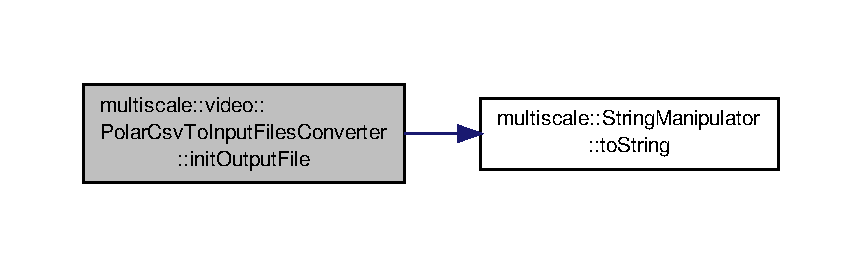
\includegraphics[width=350pt]{classmultiscale_1_1video_1_1PolarCsvToInputFilesConverter_a03d74df6e7a0b18c5099eb39f3e4fc7c_cgraph}
\end{center}
\end{figure}


\hypertarget{classmultiscale_1_1video_1_1PolarCsvToInputFilesConverter_a66168d7550e656dccf01a473ed2708f0}{\index{multiscale\-::video\-::\-Polar\-Csv\-To\-Input\-Files\-Converter@{multiscale\-::video\-::\-Polar\-Csv\-To\-Input\-Files\-Converter}!process\-Input\-File@{process\-Input\-File}}
\index{process\-Input\-File@{process\-Input\-File}!multiscale::video::PolarCsvToInputFilesConverter@{multiscale\-::video\-::\-Polar\-Csv\-To\-Input\-Files\-Converter}}
\subsubsection[{process\-Input\-File}]{\setlength{\rightskip}{0pt plus 5cm}void Polar\-Csv\-To\-Input\-Files\-Converter\-::process\-Input\-File (
\begin{DoxyParamCaption}
\item[{ifstream \&}]{fin}
\end{DoxyParamCaption}
)\hspace{0.3cm}{\ttfamily [private]}}}\label{classmultiscale_1_1video_1_1PolarCsvToInputFilesConverter_a66168d7550e656dccf01a473ed2708f0}


Process the input file. 

Read the concentrations and normalise them if it is the case.


\begin{DoxyParams}{Parameters}
{\em fin} & Input file stream \\
\hline
\end{DoxyParams}


Definition at line 178 of file Polar\-Csv\-To\-Input\-Files\-Converter.\-cpp.

\hypertarget{classmultiscale_1_1video_1_1PolarCsvToInputFilesConverter_a23c483d80d7c0c8f0510595a1ab55f69}{\index{multiscale\-::video\-::\-Polar\-Csv\-To\-Input\-Files\-Converter@{multiscale\-::video\-::\-Polar\-Csv\-To\-Input\-Files\-Converter}!process\-Line@{process\-Line}}
\index{process\-Line@{process\-Line}!multiscale::video::PolarCsvToInputFilesConverter@{multiscale\-::video\-::\-Polar\-Csv\-To\-Input\-Files\-Converter}}
\subsubsection[{process\-Line}]{\setlength{\rightskip}{0pt plus 5cm}void Polar\-Csv\-To\-Input\-Files\-Converter\-::process\-Line (
\begin{DoxyParamCaption}
\item[{const string \&}]{line, }
\item[{unsigned int}]{output\-Index}
\end{DoxyParamCaption}
)\hspace{0.3cm}{\ttfamily [private]}}}\label{classmultiscale_1_1video_1_1PolarCsvToInputFilesConverter_a23c483d80d7c0c8f0510595a1ab55f69}


Process the provided line. 


\begin{DoxyParams}{Parameters}
{\em line} & Line \\
\hline
{\em output\-Index} & Index integrated in the name of the output file \\
\hline
\end{DoxyParams}


Definition at line 193 of file Polar\-Csv\-To\-Input\-Files\-Converter.\-cpp.



References O\-U\-T\-P\-U\-T\-\_\-\-S\-E\-P\-A\-R\-A\-T\-O\-R.

\hypertarget{classmultiscale_1_1video_1_1PolarCsvToInputFilesConverter_a2ab8a181fa30c720d4ee87c188770bcc}{\index{multiscale\-::video\-::\-Polar\-Csv\-To\-Input\-Files\-Converter@{multiscale\-::video\-::\-Polar\-Csv\-To\-Input\-Files\-Converter}!split\-First\-Part\-In\-Concentrations@{split\-First\-Part\-In\-Concentrations}}
\index{split\-First\-Part\-In\-Concentrations@{split\-First\-Part\-In\-Concentrations}!multiscale::video::PolarCsvToInputFilesConverter@{multiscale\-::video\-::\-Polar\-Csv\-To\-Input\-Files\-Converter}}
\subsubsection[{split\-First\-Part\-In\-Concentrations}]{\setlength{\rightskip}{0pt plus 5cm}void Polar\-Csv\-To\-Input\-Files\-Converter\-::split\-First\-Part\-In\-Concentrations (
\begin{DoxyParamCaption}
\item[{vector$<$ double $>$ \&}]{concentrations, }
\item[{const vector$<$ string $>$ \&}]{tokens, }
\item[{unsigned int}]{circle\-Index}
\end{DoxyParamCaption}
)\hspace{0.3cm}{\ttfamily [private]}}}\label{classmultiscale_1_1video_1_1PolarCsvToInputFilesConverter_a2ab8a181fa30c720d4ee87c188770bcc}


Split first part of the line (i.\-e. part representing the origin) into concentrations. 


\begin{DoxyParams}{Parameters}
{\em concentrations} & Concentrations extracted from tokens \\
\hline
{\em tokens} & Tokens representing the line \\
\hline
{\em circle\-Index} & Index of the current concentric circle \\
\hline
\end{DoxyParams}


Definition at line 237 of file Polar\-Csv\-To\-Input\-Files\-Converter.\-cpp.

\hypertarget{classmultiscale_1_1video_1_1PolarCsvToInputFilesConverter_af2d31d32cdba42aeb5589b3faab315ad}{\index{multiscale\-::video\-::\-Polar\-Csv\-To\-Input\-Files\-Converter@{multiscale\-::video\-::\-Polar\-Csv\-To\-Input\-Files\-Converter}!split\-Line\-In\-Concentrations@{split\-Line\-In\-Concentrations}}
\index{split\-Line\-In\-Concentrations@{split\-Line\-In\-Concentrations}!multiscale::video::PolarCsvToInputFilesConverter@{multiscale\-::video\-::\-Polar\-Csv\-To\-Input\-Files\-Converter}}
\subsubsection[{split\-Line\-In\-Concentrations}]{\setlength{\rightskip}{0pt plus 5cm}vector$<$ double $>$ Polar\-Csv\-To\-Input\-Files\-Converter\-::split\-Line\-In\-Concentrations (
\begin{DoxyParamCaption}
\item[{const string \&}]{line, }
\item[{double \&}]{simulation\-Time}
\end{DoxyParamCaption}
)\hspace{0.3cm}{\ttfamily [private]}}}\label{classmultiscale_1_1video_1_1PolarCsvToInputFilesConverter_af2d31d32cdba42aeb5589b3faab315ad}


Split the line in concentrations. 


\begin{DoxyParams}{Parameters}
{\em line} & Line \\
\hline
{\em simulation\-Time} & Simulation time associated with the line \\
\hline
\end{DoxyParams}


Definition at line 212 of file Polar\-Csv\-To\-Input\-Files\-Converter.\-cpp.



References I\-N\-P\-U\-T\-\_\-\-F\-I\-L\-E\-\_\-\-S\-E\-P\-A\-R\-A\-T\-O\-R, and multiscale\-::\-String\-Manipulator\-::split().



Here is the call graph for this function\-:\nopagebreak
\begin{figure}[H]
\begin{center}
\leavevmode
\includegraphics[width=350pt]{classmultiscale_1_1video_1_1PolarCsvToInputFilesConverter_af2d31d32cdba42aeb5589b3faab315ad_cgraph}
\end{center}
\end{figure}


\hypertarget{classmultiscale_1_1video_1_1PolarCsvToInputFilesConverter_a84994d623303296509326707fa397f29}{\index{multiscale\-::video\-::\-Polar\-Csv\-To\-Input\-Files\-Converter@{multiscale\-::video\-::\-Polar\-Csv\-To\-Input\-Files\-Converter}!split\-Other\-Parts\-In\-Concentrations@{split\-Other\-Parts\-In\-Concentrations}}
\index{split\-Other\-Parts\-In\-Concentrations@{split\-Other\-Parts\-In\-Concentrations}!multiscale::video::PolarCsvToInputFilesConverter@{multiscale\-::video\-::\-Polar\-Csv\-To\-Input\-Files\-Converter}}
\subsubsection[{split\-Other\-Parts\-In\-Concentrations}]{\setlength{\rightskip}{0pt plus 5cm}void Polar\-Csv\-To\-Input\-Files\-Converter\-::split\-Other\-Parts\-In\-Concentrations (
\begin{DoxyParamCaption}
\item[{vector$<$ double $>$ \&}]{concentrations, }
\item[{const vector$<$ string $>$ \&}]{tokens, }
\item[{unsigned int}]{circle\-Index}
\end{DoxyParamCaption}
)\hspace{0.3cm}{\ttfamily [private]}}}\label{classmultiscale_1_1video_1_1PolarCsvToInputFilesConverter_a84994d623303296509326707fa397f29}


Split other parts of the line (i.\-e. non-\/first part) into concentrations. 


\begin{DoxyParams}{Parameters}
{\em concentrations} & Concentrations extracted from tokens \\
\hline
{\em tokens} & Tokens representing the line \\
\hline
{\em circle\-Index} & Index of the current concentric circle \\
\hline
\end{DoxyParams}


Definition at line 251 of file Polar\-Csv\-To\-Input\-Files\-Converter.\-cpp.

\hypertarget{classmultiscale_1_1video_1_1PolarCsvToInputFilesConverter_ae624c0a8fe97d266cbc127d64af707de}{\index{multiscale\-::video\-::\-Polar\-Csv\-To\-Input\-Files\-Converter@{multiscale\-::video\-::\-Polar\-Csv\-To\-Input\-Files\-Converter}!update\-Maximum\-Concentration@{update\-Maximum\-Concentration}}
\index{update\-Maximum\-Concentration@{update\-Maximum\-Concentration}!multiscale::video::PolarCsvToInputFilesConverter@{multiscale\-::video\-::\-Polar\-Csv\-To\-Input\-Files\-Converter}}
\subsubsection[{update\-Maximum\-Concentration}]{\setlength{\rightskip}{0pt plus 5cm}void Polar\-Csv\-To\-Input\-Files\-Converter\-::update\-Maximum\-Concentration (
\begin{DoxyParamCaption}
\item[{const string \&}]{line, }
\item[{double \&}]{maximum\-Concentration}
\end{DoxyParamCaption}
)\hspace{0.3cm}{\ttfamily [private]}}}\label{classmultiscale_1_1video_1_1PolarCsvToInputFilesConverter_ae624c0a8fe97d266cbc127d64af707de}


Update the maximum concentration if the values from the given line are greater than it. 


\begin{DoxyParams}{Parameters}
{\em line} & Line from input file \\
\hline
{\em maximum\-Concentration} & The maximum concentration \\
\hline
\end{DoxyParams}


Definition at line 340 of file Polar\-Csv\-To\-Input\-Files\-Converter.\-cpp.

\hypertarget{classmultiscale_1_1video_1_1PolarCsvToInputFilesConverter_af612ef958fd3656f2c477d4d8e81244a}{\index{multiscale\-::video\-::\-Polar\-Csv\-To\-Input\-Files\-Converter@{multiscale\-::video\-::\-Polar\-Csv\-To\-Input\-Files\-Converter}!validate\-Input@{validate\-Input}}
\index{validate\-Input@{validate\-Input}!multiscale::video::PolarCsvToInputFilesConverter@{multiscale\-::video\-::\-Polar\-Csv\-To\-Input\-Files\-Converter}}
\subsubsection[{validate\-Input}]{\setlength{\rightskip}{0pt plus 5cm}void Polar\-Csv\-To\-Input\-Files\-Converter\-::validate\-Input (
\begin{DoxyParamCaption}
\item[{ifstream \&}]{fin}
\end{DoxyParamCaption}
)\hspace{0.3cm}{\ttfamily [private]}}}\label{classmultiscale_1_1video_1_1PolarCsvToInputFilesConverter_af612ef958fd3656f2c477d4d8e81244a}


Validate the input. 


\begin{DoxyParams}{Parameters}
{\em fin} & Input file stream \\
\hline
\end{DoxyParams}


Definition at line 134 of file Polar\-Csv\-To\-Input\-Files\-Converter.\-cpp.



References E\-R\-R\-\_\-\-I\-N\-P\-U\-T\-\_\-\-O\-P\-E\-N.

\hypertarget{classmultiscale_1_1video_1_1PolarCsvToInputFilesConverter_a71741de958cfecc133a303ea3a5af22c}{\index{multiscale\-::video\-::\-Polar\-Csv\-To\-Input\-Files\-Converter@{multiscale\-::video\-::\-Polar\-Csv\-To\-Input\-Files\-Converter}!validate\-Input\-Line@{validate\-Input\-Line}}
\index{validate\-Input\-Line@{validate\-Input\-Line}!multiscale::video::PolarCsvToInputFilesConverter@{multiscale\-::video\-::\-Polar\-Csv\-To\-Input\-Files\-Converter}}
\subsubsection[{validate\-Input\-Line}]{\setlength{\rightskip}{0pt plus 5cm}void Polar\-Csv\-To\-Input\-Files\-Converter\-::validate\-Input\-Line (
\begin{DoxyParamCaption}
\item[{const string \&}]{line, }
\item[{unsigned int}]{line\-Number}
\end{DoxyParamCaption}
)\hspace{0.3cm}{\ttfamily [private]}}}\label{classmultiscale_1_1video_1_1PolarCsvToInputFilesConverter_a71741de958cfecc133a303ea3a5af22c}


Validate the provided line identified by a line number. 


\begin{DoxyParams}{Parameters}
{\em line} & Line from input file \\
\hline
{\em line\-Number} & Number of the line \\
\hline
\end{DoxyParams}


Definition at line 158 of file Polar\-Csv\-To\-Input\-Files\-Converter.\-cpp.



References E\-R\-R\-\_\-\-I\-N\-V\-A\-L\-I\-D\-\_\-\-V\-A\-L\-U\-E\-\_\-\-L\-I\-N\-E, E\-R\-R\-\_\-\-I\-N\-V\-A\-L\-I\-D\-\_\-\-V\-A\-L\-U\-E\-\_\-\-T\-O\-K\-E\-N, E\-R\-R\-\_\-\-N\-R\-\_\-\-C\-O\-N\-C\-E\-N\-T\-R\-A\-T\-I\-O\-N\-S, I\-N\-P\-U\-T\-\_\-\-F\-I\-L\-E\-\_\-\-S\-E\-P\-A\-R\-A\-T\-O\-R, and multiscale\-::\-String\-Manipulator\-::split().



Here is the call graph for this function\-:\nopagebreak
\begin{figure}[H]
\begin{center}
\leavevmode
\includegraphics[width=350pt]{classmultiscale_1_1video_1_1PolarCsvToInputFilesConverter_a71741de958cfecc133a303ea3a5af22c_cgraph}
\end{center}
\end{figure}


\hypertarget{classmultiscale_1_1video_1_1PolarCsvToInputFilesConverter_a95a32c02de43f1837f3592e4b9f03b48}{\index{multiscale\-::video\-::\-Polar\-Csv\-To\-Input\-Files\-Converter@{multiscale\-::video\-::\-Polar\-Csv\-To\-Input\-Files\-Converter}!validate\-Selected\-Concentration\-Index@{validate\-Selected\-Concentration\-Index}}
\index{validate\-Selected\-Concentration\-Index@{validate\-Selected\-Concentration\-Index}!multiscale::video::PolarCsvToInputFilesConverter@{multiscale\-::video\-::\-Polar\-Csv\-To\-Input\-Files\-Converter}}
\subsubsection[{validate\-Selected\-Concentration\-Index}]{\setlength{\rightskip}{0pt plus 5cm}void Polar\-Csv\-To\-Input\-Files\-Converter\-::validate\-Selected\-Concentration\-Index (
\begin{DoxyParamCaption}
{}
\end{DoxyParamCaption}
)\hspace{0.3cm}{\ttfamily [private]}}}\label{classmultiscale_1_1video_1_1PolarCsvToInputFilesConverter_a95a32c02de43f1837f3592e4b9f03b48}


Validate the selected concentration index in case of more than one concentration for each position. 



Definition at line 128 of file Polar\-Csv\-To\-Input\-Files\-Converter.\-cpp.



References E\-R\-R\-\_\-\-S\-E\-L\-E\-C\-T\-E\-D\-\_\-\-C\-O\-N\-C\-E\-N\-T\-R\-A\-T\-I\-O\-N\-\_\-\-I\-N\-D\-E\-X.



\subsection{Member Data Documentation}
\hypertarget{classmultiscale_1_1video_1_1PolarCsvToInputFilesConverter_ad4cf12c7f3951f0bb388939797cbcc0c}{\index{multiscale\-::video\-::\-Polar\-Csv\-To\-Input\-Files\-Converter@{multiscale\-::video\-::\-Polar\-Csv\-To\-Input\-Files\-Converter}!circles\-Iterator@{circles\-Iterator}}
\index{circles\-Iterator@{circles\-Iterator}!multiscale::video::PolarCsvToInputFilesConverter@{multiscale\-::video\-::\-Polar\-Csv\-To\-Input\-Files\-Converter}}
\subsubsection[{circles\-Iterator}]{\setlength{\rightskip}{0pt plus 5cm}{\bf Number\-Iterator}$\ast$ multiscale\-::video\-::\-Polar\-Csv\-To\-Input\-Files\-Converter\-::circles\-Iterator\hspace{0.3cm}{\ttfamily [private]}}}\label{classmultiscale_1_1video_1_1PolarCsvToInputFilesConverter_ad4cf12c7f3951f0bb388939797cbcc0c}
Iterator over the number of concentric circles 

Definition at line 57 of file Polar\-Csv\-To\-Input\-Files\-Converter.\-hpp.

\hypertarget{classmultiscale_1_1video_1_1PolarCsvToInputFilesConverter_afd9f17e6ba2dc46b920ab28538278362}{\index{multiscale\-::video\-::\-Polar\-Csv\-To\-Input\-Files\-Converter@{multiscale\-::video\-::\-Polar\-Csv\-To\-Input\-Files\-Converter}!concentrations\-Index@{concentrations\-Index}}
\index{concentrations\-Index@{concentrations\-Index}!multiscale::video::PolarCsvToInputFilesConverter@{multiscale\-::video\-::\-Polar\-Csv\-To\-Input\-Files\-Converter}}
\subsubsection[{concentrations\-Index}]{\setlength{\rightskip}{0pt plus 5cm}unsigned int multiscale\-::video\-::\-Polar\-Csv\-To\-Input\-Files\-Converter\-::concentrations\-Index\hspace{0.3cm}{\ttfamily [private]}}}\label{classmultiscale_1_1video_1_1PolarCsvToInputFilesConverter_afd9f17e6ba2dc46b920ab28538278362}
Index of the current concentration 

Definition at line 44 of file Polar\-Csv\-To\-Input\-Files\-Converter.\-hpp.

\hypertarget{classmultiscale_1_1video_1_1PolarCsvToInputFilesConverter_a7b33b6d00b5e0d809f4fb0d76985ab59}{\index{multiscale\-::video\-::\-Polar\-Csv\-To\-Input\-Files\-Converter@{multiscale\-::video\-::\-Polar\-Csv\-To\-Input\-Files\-Converter}!input\-Filepath@{input\-Filepath}}
\index{input\-Filepath@{input\-Filepath}!multiscale::video::PolarCsvToInputFilesConverter@{multiscale\-::video\-::\-Polar\-Csv\-To\-Input\-Files\-Converter}}
\subsubsection[{input\-Filepath}]{\setlength{\rightskip}{0pt plus 5cm}string multiscale\-::video\-::\-Polar\-Csv\-To\-Input\-Files\-Converter\-::input\-Filepath\hspace{0.3cm}{\ttfamily [private]}}}\label{classmultiscale_1_1video_1_1PolarCsvToInputFilesConverter_a7b33b6d00b5e0d809f4fb0d76985ab59}
Path to the input file 

Definition at line 37 of file Polar\-Csv\-To\-Input\-Files\-Converter.\-hpp.

\hypertarget{classmultiscale_1_1video_1_1PolarCsvToInputFilesConverter_a89b7dce2825cd5c8c45a1e6f19770e5f}{\index{multiscale\-::video\-::\-Polar\-Csv\-To\-Input\-Files\-Converter@{multiscale\-::video\-::\-Polar\-Csv\-To\-Input\-Files\-Converter}!maximum\-Concentration@{maximum\-Concentration}}
\index{maximum\-Concentration@{maximum\-Concentration}!multiscale::video::PolarCsvToInputFilesConverter@{multiscale\-::video\-::\-Polar\-Csv\-To\-Input\-Files\-Converter}}
\subsubsection[{maximum\-Concentration}]{\setlength{\rightskip}{0pt plus 5cm}double multiscale\-::video\-::\-Polar\-Csv\-To\-Input\-Files\-Converter\-::maximum\-Concentration\hspace{0.3cm}{\ttfamily [private]}}}\label{classmultiscale_1_1video_1_1PolarCsvToInputFilesConverter_a89b7dce2825cd5c8c45a1e6f19770e5f}
The maximum concentration in the input file 

Definition at line 55 of file Polar\-Csv\-To\-Input\-Files\-Converter.\-hpp.

\hypertarget{classmultiscale_1_1video_1_1PolarCsvToInputFilesConverter_a3a9301788514c50c295ca113a4114938}{\index{multiscale\-::video\-::\-Polar\-Csv\-To\-Input\-Files\-Converter@{multiscale\-::video\-::\-Polar\-Csv\-To\-Input\-Files\-Converter}!nr\-Of\-Concentrations\-For\-Position@{nr\-Of\-Concentrations\-For\-Position}}
\index{nr\-Of\-Concentrations\-For\-Position@{nr\-Of\-Concentrations\-For\-Position}!multiscale::video::PolarCsvToInputFilesConverter@{multiscale\-::video\-::\-Polar\-Csv\-To\-Input\-Files\-Converter}}
\subsubsection[{nr\-Of\-Concentrations\-For\-Position}]{\setlength{\rightskip}{0pt plus 5cm}unsigned int multiscale\-::video\-::\-Polar\-Csv\-To\-Input\-Files\-Converter\-::nr\-Of\-Concentrations\-For\-Position\hspace{0.3cm}{\ttfamily [private]}}}\label{classmultiscale_1_1video_1_1PolarCsvToInputFilesConverter_a3a9301788514c50c295ca113a4114938}
Number of concentrations for each position 

Definition at line 42 of file Polar\-Csv\-To\-Input\-Files\-Converter.\-hpp.

\hypertarget{classmultiscale_1_1video_1_1PolarCsvToInputFilesConverter_a7aa37d18880e822369cbe118a093e24f}{\index{multiscale\-::video\-::\-Polar\-Csv\-To\-Input\-Files\-Converter@{multiscale\-::video\-::\-Polar\-Csv\-To\-Input\-Files\-Converter}!nr\-Of\-Concentric\-Circles@{nr\-Of\-Concentric\-Circles}}
\index{nr\-Of\-Concentric\-Circles@{nr\-Of\-Concentric\-Circles}!multiscale::video::PolarCsvToInputFilesConverter@{multiscale\-::video\-::\-Polar\-Csv\-To\-Input\-Files\-Converter}}
\subsubsection[{nr\-Of\-Concentric\-Circles}]{\setlength{\rightskip}{0pt plus 5cm}unsigned int multiscale\-::video\-::\-Polar\-Csv\-To\-Input\-Files\-Converter\-::nr\-Of\-Concentric\-Circles\hspace{0.3cm}{\ttfamily [private]}}}\label{classmultiscale_1_1video_1_1PolarCsvToInputFilesConverter_a7aa37d18880e822369cbe118a093e24f}
Number of concentric circles 

Definition at line 40 of file Polar\-Csv\-To\-Input\-Files\-Converter.\-hpp.

\hypertarget{classmultiscale_1_1video_1_1PolarCsvToInputFilesConverter_a9246a2c9749602af145d5579bde8a9d1}{\index{multiscale\-::video\-::\-Polar\-Csv\-To\-Input\-Files\-Converter@{multiscale\-::video\-::\-Polar\-Csv\-To\-Input\-Files\-Converter}!nr\-Of\-Sectors@{nr\-Of\-Sectors}}
\index{nr\-Of\-Sectors@{nr\-Of\-Sectors}!multiscale::video::PolarCsvToInputFilesConverter@{multiscale\-::video\-::\-Polar\-Csv\-To\-Input\-Files\-Converter}}
\subsubsection[{nr\-Of\-Sectors}]{\setlength{\rightskip}{0pt plus 5cm}unsigned int multiscale\-::video\-::\-Polar\-Csv\-To\-Input\-Files\-Converter\-::nr\-Of\-Sectors\hspace{0.3cm}{\ttfamily [private]}}}\label{classmultiscale_1_1video_1_1PolarCsvToInputFilesConverter_a9246a2c9749602af145d5579bde8a9d1}
Number of sectors 

Definition at line 41 of file Polar\-Csv\-To\-Input\-Files\-Converter.\-hpp.

\hypertarget{classmultiscale_1_1video_1_1PolarCsvToInputFilesConverter_a1033d31c9bfc7ccad08337c7b0fa6e6e}{\index{multiscale\-::video\-::\-Polar\-Csv\-To\-Input\-Files\-Converter@{multiscale\-::video\-::\-Polar\-Csv\-To\-Input\-Files\-Converter}!output\-Filepath@{output\-Filepath}}
\index{output\-Filepath@{output\-Filepath}!multiscale::video::PolarCsvToInputFilesConverter@{multiscale\-::video\-::\-Polar\-Csv\-To\-Input\-Files\-Converter}}
\subsubsection[{output\-Filepath}]{\setlength{\rightskip}{0pt plus 5cm}string multiscale\-::video\-::\-Polar\-Csv\-To\-Input\-Files\-Converter\-::output\-Filepath\hspace{0.3cm}{\ttfamily [private]}}}\label{classmultiscale_1_1video_1_1PolarCsvToInputFilesConverter_a1033d31c9bfc7ccad08337c7b0fa6e6e}
Path to the output file 

Definition at line 38 of file Polar\-Csv\-To\-Input\-Files\-Converter.\-hpp.

\hypertarget{classmultiscale_1_1video_1_1PolarCsvToInputFilesConverter_aa6895c1613a551cd05195f05ae51862b}{\index{multiscale\-::video\-::\-Polar\-Csv\-To\-Input\-Files\-Converter@{multiscale\-::video\-::\-Polar\-Csv\-To\-Input\-Files\-Converter}!sectors\-Iterator@{sectors\-Iterator}}
\index{sectors\-Iterator@{sectors\-Iterator}!multiscale::video::PolarCsvToInputFilesConverter@{multiscale\-::video\-::\-Polar\-Csv\-To\-Input\-Files\-Converter}}
\subsubsection[{sectors\-Iterator}]{\setlength{\rightskip}{0pt plus 5cm}{\bf Number\-Iterator}$\ast$ multiscale\-::video\-::\-Polar\-Csv\-To\-Input\-Files\-Converter\-::sectors\-Iterator\hspace{0.3cm}{\ttfamily [private]}}}\label{classmultiscale_1_1video_1_1PolarCsvToInputFilesConverter_aa6895c1613a551cd05195f05ae51862b}
Iterator over the number of sectors 

Definition at line 58 of file Polar\-Csv\-To\-Input\-Files\-Converter.\-hpp.

\hypertarget{classmultiscale_1_1video_1_1PolarCsvToInputFilesConverter_a121d592659f9f5075c8c78aa46c2950c}{\index{multiscale\-::video\-::\-Polar\-Csv\-To\-Input\-Files\-Converter@{multiscale\-::video\-::\-Polar\-Csv\-To\-Input\-Files\-Converter}!selected\-Concentration\-Index@{selected\-Concentration\-Index}}
\index{selected\-Concentration\-Index@{selected\-Concentration\-Index}!multiscale::video::PolarCsvToInputFilesConverter@{multiscale\-::video\-::\-Polar\-Csv\-To\-Input\-Files\-Converter}}
\subsubsection[{selected\-Concentration\-Index}]{\setlength{\rightskip}{0pt plus 5cm}unsigned int multiscale\-::video\-::\-Polar\-Csv\-To\-Input\-Files\-Converter\-::selected\-Concentration\-Index\hspace{0.3cm}{\ttfamily [private]}}}\label{classmultiscale_1_1video_1_1PolarCsvToInputFilesConverter_a121d592659f9f5075c8c78aa46c2950c}
\begin{DoxyVerb}    Index of the concentration A in case the number of
\end{DoxyVerb}
 concentrations for each position is greater than 1

final\-Concentration = A / (A1 + A2 + ... + A\-N), where N is the number of concentrations for each position 

Definition at line 46 of file Polar\-Csv\-To\-Input\-Files\-Converter.\-hpp.

\hypertarget{classmultiscale_1_1video_1_1PolarCsvToInputFilesConverter_af07bf56fc39bb226a6e2596f35ada0d7}{\index{multiscale\-::video\-::\-Polar\-Csv\-To\-Input\-Files\-Converter@{multiscale\-::video\-::\-Polar\-Csv\-To\-Input\-Files\-Converter}!use\-Log\-Scaling@{use\-Log\-Scaling}}
\index{use\-Log\-Scaling@{use\-Log\-Scaling}!multiscale::video::PolarCsvToInputFilesConverter@{multiscale\-::video\-::\-Polar\-Csv\-To\-Input\-Files\-Converter}}
\subsubsection[{use\-Log\-Scaling}]{\setlength{\rightskip}{0pt plus 5cm}bool multiscale\-::video\-::\-Polar\-Csv\-To\-Input\-Files\-Converter\-::use\-Log\-Scaling\hspace{0.3cm}{\ttfamily [private]}}}\label{classmultiscale_1_1video_1_1PolarCsvToInputFilesConverter_af07bf56fc39bb226a6e2596f35ada0d7}
Flag for using logarithmic scaling for concentrations or not 

Definition at line 53 of file Polar\-Csv\-To\-Input\-Files\-Converter.\-hpp.



The documentation for this class was generated from the following files\-:\begin{DoxyCompactItemize}
\item 
include/multiscale/video/circular/\hyperlink{PolarCsvToInputFilesConverter_8hpp}{Polar\-Csv\-To\-Input\-Files\-Converter.\-hpp}\item 
src/multiscale/video/circular/\hyperlink{PolarCsvToInputFilesConverter_8cpp}{Polar\-Csv\-To\-Input\-Files\-Converter.\-cpp}\end{DoxyCompactItemize}

\hypertarget{classmultiscale_1_1video_1_1PolarGnuplotScriptGenerator}{\section{multiscale\-:\-:video\-:\-:Polar\-Gnuplot\-Script\-Generator Class Reference}
\label{classmultiscale_1_1video_1_1PolarGnuplotScriptGenerator}\index{multiscale\-::video\-::\-Polar\-Gnuplot\-Script\-Generator@{multiscale\-::video\-::\-Polar\-Gnuplot\-Script\-Generator}}
}


Gnuplot script generator from the provided annular sectors.  




{\ttfamily \#include $<$Polar\-Gnuplot\-Script\-Generator.\-hpp$>$}



Collaboration diagram for multiscale\-:\-:video\-:\-:Polar\-Gnuplot\-Script\-Generator\-:\nopagebreak
\begin{figure}[H]
\begin{center}
\leavevmode
\includegraphics[width=298pt]{classmultiscale_1_1video_1_1PolarGnuplotScriptGenerator__coll__graph}
\end{center}
\end{figure}
\subsection*{Static Public Member Functions}
\begin{DoxyCompactItemize}
\item 
static void \hyperlink{classmultiscale_1_1video_1_1PolarGnuplotScriptGenerator_a9e60fa7dd9c47dc89cdce30a39175a6e}{generate\-Script} (const vector$<$ \hyperlink{classmultiscale_1_1video_1_1AnnularSector}{Annular\-Sector} $>$ \&annular\-Sectors, double simulation\-Time, const string \&output\-Filepath)
\begin{DoxyCompactList}\small\item\em Generate the script. \end{DoxyCompactList}\end{DoxyCompactItemize}
\subsection*{Static Private Member Functions}
\begin{DoxyCompactItemize}
\item 
static void \hyperlink{classmultiscale_1_1video_1_1PolarGnuplotScriptGenerator_abad924831da9046dc757a7508f47ce55}{generate\-Header} (ofstream \&fout, const string \&output\-Filepath, double simulation\-Time)
\begin{DoxyCompactList}\small\item\em Generate the header of the script. \end{DoxyCompactList}\item 
static void \hyperlink{classmultiscale_1_1video_1_1PolarGnuplotScriptGenerator_a5386b0f2c6286c709c3084c5101963c6}{generate\-Body} (const vector$<$ \hyperlink{classmultiscale_1_1video_1_1AnnularSector}{Annular\-Sector} $>$ \&annular\-Sectors, ofstream \&fout)
\begin{DoxyCompactList}\small\item\em Generate the body/content of the script. \end{DoxyCompactList}\item 
static void \hyperlink{classmultiscale_1_1video_1_1PolarGnuplotScriptGenerator_af760c3b80b2d8966d7fbea00b97e3785}{generate\-Footer} (ofstream \&fout)
\begin{DoxyCompactList}\small\item\em Generate the footer of the script. \end{DoxyCompactList}\item 
static void \hyperlink{classmultiscale_1_1video_1_1PolarGnuplotScriptGenerator_a9d10aa501cb749ef09a5c3019406ddc1}{output\-Header} (ifstream \&fin, const string \&output\-Filename, double simulation\-Time, ofstream \&fout)
\begin{DoxyCompactList}\small\item\em Output the header of the script. \end{DoxyCompactList}\item 
static void \hyperlink{classmultiscale_1_1video_1_1PolarGnuplotScriptGenerator_a5ccc1caca243f48e7cb7bc1083bd07a3}{output\-Content} (const vector$<$ \hyperlink{classmultiscale_1_1video_1_1AnnularSector}{Annular\-Sector} $>$ \&annular\-Sectors, const string \&content\-Template, ofstream \&fout)
\begin{DoxyCompactList}\small\item\em Output the content of the script. \end{DoxyCompactList}\item 
static void \hyperlink{classmultiscale_1_1video_1_1PolarGnuplotScriptGenerator_ad572033c31036eb4b3fd041eaf70ec5f}{output\-Footer} (ifstream \&fin, ofstream \&fout)
\begin{DoxyCompactList}\small\item\em Output the footer of the script. \end{DoxyCompactList}\item 
static string \hyperlink{classmultiscale_1_1video_1_1PolarGnuplotScriptGenerator_a539bef80a3f6313a0df4c72107075e35}{read\-Content\-Template} (ifstream \&fin)
\begin{DoxyCompactList}\small\item\em Read content template. \end{DoxyCompactList}\end{DoxyCompactItemize}
\subsection*{Static Private Attributes}
\begin{DoxyCompactItemize}
\item 
static const string \hyperlink{classmultiscale_1_1video_1_1PolarGnuplotScriptGenerator_acd5fb0e27c9f7857d68b7ec9cb62fb74}{H\-E\-A\-D\-E\-R\-\_\-\-I\-N} = \char`\"{}config/video/circular/header.\-in\char`\"{}
\item 
static const string \hyperlink{classmultiscale_1_1video_1_1PolarGnuplotScriptGenerator_ad8fb67fe439899d85924bd7339b7d08c}{C\-O\-N\-T\-E\-N\-T\-\_\-\-I\-N} = \char`\"{}config/video/circular/content.\-in\char`\"{}
\item 
static const string \hyperlink{classmultiscale_1_1video_1_1PolarGnuplotScriptGenerator_aae225d7380fd7815efa1aed69087e6b0}{F\-O\-O\-T\-E\-R\-\_\-\-I\-N} = \char`\"{}config/video/circular/footer.\-in\char`\"{}
\item 
static const string \hyperlink{classmultiscale_1_1video_1_1PolarGnuplotScriptGenerator_af5f0a7c41016915eaa5756695f17fd4a}{R\-E\-P\-L\-A\-C\-E\-\_\-\-H\-E\-A\-D\-E\-R\-\_\-\-F\-I\-L\-E\-N\-A\-M\-E} = \char`\"{}O\-U\-T\-P\-U\-T\-\_\-\-F\-I\-L\-E\-N\-A\-M\-E\char`\"{}
\item 
static const string \hyperlink{classmultiscale_1_1video_1_1PolarGnuplotScriptGenerator_ab06a56e8ac6c117d9a3d1279bd114941}{R\-E\-P\-L\-A\-C\-E\-\_\-\-H\-E\-A\-D\-E\-R\-\_\-\-S\-I\-M\-\_\-\-T\-I\-M\-E} = \char`\"{}O\-U\-T\-P\-U\-T\-\_\-\-S\-I\-M\-\_\-\-T\-I\-M\-E\char`\"{}
\item 
static const string \hyperlink{classmultiscale_1_1video_1_1PolarGnuplotScriptGenerator_a0899b28bb340224529c005d262ffb09f}{R\-E\-P\-L\-A\-C\-E\-\_\-\-C\-O\-N\-T\-E\-N\-T\-\_\-\-I\-N\-D\-E\-X} = \char`\"{}O\-B\-J\-\_\-\-I\-N\-D\-E\-X\char`\"{}
\item 
static const string \hyperlink{classmultiscale_1_1video_1_1PolarGnuplotScriptGenerator_a2fcfd2afdf3aa1f35b18fc04946f40d2}{R\-E\-P\-L\-A\-C\-E\-\_\-\-C\-O\-N\-T\-E\-N\-T\-\_\-\-R\-A\-D\-I\-U\-S} = \char`\"{}O\-B\-J\-\_\-\-E\-N\-D\-\_\-\-R\-A\-D\-I\-U\-S\char`\"{}
\item 
static const string \hyperlink{classmultiscale_1_1video_1_1PolarGnuplotScriptGenerator_acb8550fbb7a7f199d01d77622b054e10}{R\-E\-P\-L\-A\-C\-E\-\_\-\-C\-O\-N\-T\-E\-N\-T\-\_\-\-S\-T\-A\-R\-T\-\_\-\-A\-N\-G\-L\-E} = \char`\"{}O\-B\-J\-\_\-\-S\-T\-A\-R\-T\-\_\-\-A\-N\-G\-L\-E\char`\"{}
\item 
static const string \hyperlink{classmultiscale_1_1video_1_1PolarGnuplotScriptGenerator_aeb30ca67d1a36b859159849f64f1804d}{R\-E\-P\-L\-A\-C\-E\-\_\-\-C\-O\-N\-T\-E\-N\-T\-\_\-\-E\-N\-D\-\_\-\-A\-N\-G\-L\-E} = \char`\"{}O\-B\-J\-\_\-\-E\-N\-D\-\_\-\-A\-N\-G\-L\-E\char`\"{}
\item 
static const string \hyperlink{classmultiscale_1_1video_1_1PolarGnuplotScriptGenerator_a4b875e1e820e529622399437e098c6eb}{R\-E\-P\-L\-A\-C\-E\-\_\-\-C\-O\-N\-T\-E\-N\-T\-\_\-\-C\-O\-N\-C\-E\-N\-T\-R\-A\-T\-I\-O\-N} = \char`\"{}O\-B\-J\-\_\-\-C\-O\-N\-C\-E\-N\-T\-R\-A\-T\-I\-O\-N\char`\"{}
\item 
static const string \hyperlink{classmultiscale_1_1video_1_1PolarGnuplotScriptGenerator_ab7c725911d4456addf22db345b622057}{G\-N\-U\-P\-L\-O\-T\-\_\-\-E\-X\-T\-E\-N\-S\-I\-O\-N} = \char`\"{}.plt\char`\"{}
\end{DoxyCompactItemize}


\subsection{Detailed Description}
Gnuplot script generator from the provided annular sectors. 

Definition at line 16 of file Polar\-Gnuplot\-Script\-Generator.\-hpp.



\subsection{Member Function Documentation}
\hypertarget{classmultiscale_1_1video_1_1PolarGnuplotScriptGenerator_a5386b0f2c6286c709c3084c5101963c6}{\index{multiscale\-::video\-::\-Polar\-Gnuplot\-Script\-Generator@{multiscale\-::video\-::\-Polar\-Gnuplot\-Script\-Generator}!generate\-Body@{generate\-Body}}
\index{generate\-Body@{generate\-Body}!multiscale::video::PolarGnuplotScriptGenerator@{multiscale\-::video\-::\-Polar\-Gnuplot\-Script\-Generator}}
\subsubsection[{generate\-Body}]{\setlength{\rightskip}{0pt plus 5cm}void Polar\-Gnuplot\-Script\-Generator\-::generate\-Body (
\begin{DoxyParamCaption}
\item[{const vector$<$ {\bf Annular\-Sector} $>$ \&}]{annular\-Sectors, }
\item[{ofstream \&}]{fout}
\end{DoxyParamCaption}
)\hspace{0.3cm}{\ttfamily [static]}, {\ttfamily [private]}}}\label{classmultiscale_1_1video_1_1PolarGnuplotScriptGenerator_a5386b0f2c6286c709c3084c5101963c6}


Generate the body/content of the script. 


\begin{DoxyParams}{Parameters}
{\em annular\-Sectors} & Annular sectors \\
\hline
{\em fout} & Output file stream \\
\hline
\end{DoxyParams}


Definition at line 40 of file Polar\-Gnuplot\-Script\-Generator.\-cpp.

\hypertarget{classmultiscale_1_1video_1_1PolarGnuplotScriptGenerator_af760c3b80b2d8966d7fbea00b97e3785}{\index{multiscale\-::video\-::\-Polar\-Gnuplot\-Script\-Generator@{multiscale\-::video\-::\-Polar\-Gnuplot\-Script\-Generator}!generate\-Footer@{generate\-Footer}}
\index{generate\-Footer@{generate\-Footer}!multiscale::video::PolarGnuplotScriptGenerator@{multiscale\-::video\-::\-Polar\-Gnuplot\-Script\-Generator}}
\subsubsection[{generate\-Footer}]{\setlength{\rightskip}{0pt plus 5cm}void Polar\-Gnuplot\-Script\-Generator\-::generate\-Footer (
\begin{DoxyParamCaption}
\item[{ofstream \&}]{fout}
\end{DoxyParamCaption}
)\hspace{0.3cm}{\ttfamily [static]}, {\ttfamily [private]}}}\label{classmultiscale_1_1video_1_1PolarGnuplotScriptGenerator_af760c3b80b2d8966d7fbea00b97e3785}


Generate the footer of the script. 


\begin{DoxyParams}{Parameters}
{\em fout} & Output file stream \\
\hline
\end{DoxyParams}


Definition at line 52 of file Polar\-Gnuplot\-Script\-Generator.\-cpp.

\hypertarget{classmultiscale_1_1video_1_1PolarGnuplotScriptGenerator_abad924831da9046dc757a7508f47ce55}{\index{multiscale\-::video\-::\-Polar\-Gnuplot\-Script\-Generator@{multiscale\-::video\-::\-Polar\-Gnuplot\-Script\-Generator}!generate\-Header@{generate\-Header}}
\index{generate\-Header@{generate\-Header}!multiscale::video::PolarGnuplotScriptGenerator@{multiscale\-::video\-::\-Polar\-Gnuplot\-Script\-Generator}}
\subsubsection[{generate\-Header}]{\setlength{\rightskip}{0pt plus 5cm}void Polar\-Gnuplot\-Script\-Generator\-::generate\-Header (
\begin{DoxyParamCaption}
\item[{ofstream \&}]{fout, }
\item[{const string \&}]{output\-Filepath, }
\item[{double}]{simulation\-Time}
\end{DoxyParamCaption}
)\hspace{0.3cm}{\ttfamily [static]}, {\ttfamily [private]}}}\label{classmultiscale_1_1video_1_1PolarGnuplotScriptGenerator_abad924831da9046dc757a7508f47ce55}


Generate the header of the script. 


\begin{DoxyParams}{Parameters}
{\em fout} & Output file stream \\
\hline
{\em output\-Filepath} & Path to the output file \\
\hline
{\em simulation\-Time} & Simulation time \\
\hline
\end{DoxyParams}


Definition at line 28 of file Polar\-Gnuplot\-Script\-Generator.\-cpp.



References multiscale\-::\-String\-Manipulator\-::filename\-From\-Path().



Here is the call graph for this function\-:\nopagebreak
\begin{figure}[H]
\begin{center}
\leavevmode
\includegraphics[width=350pt]{classmultiscale_1_1video_1_1PolarGnuplotScriptGenerator_abad924831da9046dc757a7508f47ce55_cgraph}
\end{center}
\end{figure}


\hypertarget{classmultiscale_1_1video_1_1PolarGnuplotScriptGenerator_a9e60fa7dd9c47dc89cdce30a39175a6e}{\index{multiscale\-::video\-::\-Polar\-Gnuplot\-Script\-Generator@{multiscale\-::video\-::\-Polar\-Gnuplot\-Script\-Generator}!generate\-Script@{generate\-Script}}
\index{generate\-Script@{generate\-Script}!multiscale::video::PolarGnuplotScriptGenerator@{multiscale\-::video\-::\-Polar\-Gnuplot\-Script\-Generator}}
\subsubsection[{generate\-Script}]{\setlength{\rightskip}{0pt plus 5cm}void Polar\-Gnuplot\-Script\-Generator\-::generate\-Script (
\begin{DoxyParamCaption}
\item[{const vector$<$ {\bf Annular\-Sector} $>$ \&}]{annular\-Sectors, }
\item[{double}]{simulation\-Time, }
\item[{const string \&}]{output\-Filepath}
\end{DoxyParamCaption}
)\hspace{0.3cm}{\ttfamily [static]}}}\label{classmultiscale_1_1video_1_1PolarGnuplotScriptGenerator_a9e60fa7dd9c47dc89cdce30a39175a6e}


Generate the script. 


\begin{DoxyParams}{Parameters}
{\em annular\-Sectors} & Annular sectors \\
\hline
{\em simulation\-Time} & Simulation time \\
\hline
{\em output\-Filepath} & Path of the output file \\
\hline
\end{DoxyParams}


Definition at line 14 of file Polar\-Gnuplot\-Script\-Generator.\-cpp.



Referenced by multiscale\-::video\-::\-Cartesian\-To\-Polar\-Converter\-::output\-Results\-As\-Script().



Here is the caller graph for this function\-:\nopagebreak
\begin{figure}[H]
\begin{center}
\leavevmode
\includegraphics[width=350pt]{classmultiscale_1_1video_1_1PolarGnuplotScriptGenerator_a9e60fa7dd9c47dc89cdce30a39175a6e_icgraph}
\end{center}
\end{figure}


\hypertarget{classmultiscale_1_1video_1_1PolarGnuplotScriptGenerator_a5ccc1caca243f48e7cb7bc1083bd07a3}{\index{multiscale\-::video\-::\-Polar\-Gnuplot\-Script\-Generator@{multiscale\-::video\-::\-Polar\-Gnuplot\-Script\-Generator}!output\-Content@{output\-Content}}
\index{output\-Content@{output\-Content}!multiscale::video::PolarGnuplotScriptGenerator@{multiscale\-::video\-::\-Polar\-Gnuplot\-Script\-Generator}}
\subsubsection[{output\-Content}]{\setlength{\rightskip}{0pt plus 5cm}void Polar\-Gnuplot\-Script\-Generator\-::output\-Content (
\begin{DoxyParamCaption}
\item[{const vector$<$ {\bf Annular\-Sector} $>$ \&}]{annular\-Sectors, }
\item[{const string \&}]{content\-Template, }
\item[{ofstream \&}]{fout}
\end{DoxyParamCaption}
)\hspace{0.3cm}{\ttfamily [static]}, {\ttfamily [private]}}}\label{classmultiscale_1_1video_1_1PolarGnuplotScriptGenerator_a5ccc1caca243f48e7cb7bc1083bd07a3}


Output the content of the script. 


\begin{DoxyParams}{Parameters}
{\em annular\-Sectors} & Annular sectors \\
\hline
{\em content\-Template} & Template used for generating output for each annular sector \\
\hline
{\em fout} & Output file stream \\
\hline
\end{DoxyParams}


Definition at line 75 of file Polar\-Gnuplot\-Script\-Generator.\-cpp.



References multiscale\-::\-String\-Manipulator\-::replace().



Here is the call graph for this function\-:\nopagebreak
\begin{figure}[H]
\begin{center}
\leavevmode
\includegraphics[width=350pt]{classmultiscale_1_1video_1_1PolarGnuplotScriptGenerator_a5ccc1caca243f48e7cb7bc1083bd07a3_cgraph}
\end{center}
\end{figure}


\hypertarget{classmultiscale_1_1video_1_1PolarGnuplotScriptGenerator_ad572033c31036eb4b3fd041eaf70ec5f}{\index{multiscale\-::video\-::\-Polar\-Gnuplot\-Script\-Generator@{multiscale\-::video\-::\-Polar\-Gnuplot\-Script\-Generator}!output\-Footer@{output\-Footer}}
\index{output\-Footer@{output\-Footer}!multiscale::video::PolarGnuplotScriptGenerator@{multiscale\-::video\-::\-Polar\-Gnuplot\-Script\-Generator}}
\subsubsection[{output\-Footer}]{\setlength{\rightskip}{0pt plus 5cm}void Polar\-Gnuplot\-Script\-Generator\-::output\-Footer (
\begin{DoxyParamCaption}
\item[{ifstream \&}]{fin, }
\item[{ofstream \&}]{fout}
\end{DoxyParamCaption}
)\hspace{0.3cm}{\ttfamily [static]}, {\ttfamily [private]}}}\label{classmultiscale_1_1video_1_1PolarGnuplotScriptGenerator_ad572033c31036eb4b3fd041eaf70ec5f}


Output the footer of the script. 


\begin{DoxyParams}{Parameters}
{\em fin} & Input file stream \\
\hline
{\em fout} & Output file stream \\
\hline
\end{DoxyParams}


Definition at line 93 of file Polar\-Gnuplot\-Script\-Generator.\-cpp.

\hypertarget{classmultiscale_1_1video_1_1PolarGnuplotScriptGenerator_a9d10aa501cb749ef09a5c3019406ddc1}{\index{multiscale\-::video\-::\-Polar\-Gnuplot\-Script\-Generator@{multiscale\-::video\-::\-Polar\-Gnuplot\-Script\-Generator}!output\-Header@{output\-Header}}
\index{output\-Header@{output\-Header}!multiscale::video::PolarGnuplotScriptGenerator@{multiscale\-::video\-::\-Polar\-Gnuplot\-Script\-Generator}}
\subsubsection[{output\-Header}]{\setlength{\rightskip}{0pt plus 5cm}void Polar\-Gnuplot\-Script\-Generator\-::output\-Header (
\begin{DoxyParamCaption}
\item[{ifstream \&}]{fin, }
\item[{const string \&}]{output\-Filename, }
\item[{double}]{simulation\-Time, }
\item[{ofstream \&}]{fout}
\end{DoxyParamCaption}
)\hspace{0.3cm}{\ttfamily [static]}, {\ttfamily [private]}}}\label{classmultiscale_1_1video_1_1PolarGnuplotScriptGenerator_a9d10aa501cb749ef09a5c3019406ddc1}


Output the header of the script. 


\begin{DoxyParams}{Parameters}
{\em fin} & Input file stream \\
\hline
{\em output\-Filename} & Name of the output file \\
\hline
{\em simulation\-Time} & Simulation time \\
\hline
{\em fout} & Output file stream \\
\hline
\end{DoxyParams}


Definition at line 62 of file Polar\-Gnuplot\-Script\-Generator.\-cpp.



References multiscale\-::\-String\-Manipulator\-::replace().



Here is the call graph for this function\-:\nopagebreak
\begin{figure}[H]
\begin{center}
\leavevmode
\includegraphics[width=350pt]{classmultiscale_1_1video_1_1PolarGnuplotScriptGenerator_a9d10aa501cb749ef09a5c3019406ddc1_cgraph}
\end{center}
\end{figure}


\hypertarget{classmultiscale_1_1video_1_1PolarGnuplotScriptGenerator_a539bef80a3f6313a0df4c72107075e35}{\index{multiscale\-::video\-::\-Polar\-Gnuplot\-Script\-Generator@{multiscale\-::video\-::\-Polar\-Gnuplot\-Script\-Generator}!read\-Content\-Template@{read\-Content\-Template}}
\index{read\-Content\-Template@{read\-Content\-Template}!multiscale::video::PolarGnuplotScriptGenerator@{multiscale\-::video\-::\-Polar\-Gnuplot\-Script\-Generator}}
\subsubsection[{read\-Content\-Template}]{\setlength{\rightskip}{0pt plus 5cm}string Polar\-Gnuplot\-Script\-Generator\-::read\-Content\-Template (
\begin{DoxyParamCaption}
\item[{ifstream \&}]{fin}
\end{DoxyParamCaption}
)\hspace{0.3cm}{\ttfamily [static]}, {\ttfamily [private]}}}\label{classmultiscale_1_1video_1_1PolarGnuplotScriptGenerator_a539bef80a3f6313a0df4c72107075e35}


Read content template. 


\begin{DoxyParams}{Parameters}
{\em fin} & Input file stream \\
\hline
\end{DoxyParams}


Definition at line 103 of file Polar\-Gnuplot\-Script\-Generator.\-cpp.



\subsection{Member Data Documentation}
\hypertarget{classmultiscale_1_1video_1_1PolarGnuplotScriptGenerator_ad8fb67fe439899d85924bd7339b7d08c}{\index{multiscale\-::video\-::\-Polar\-Gnuplot\-Script\-Generator@{multiscale\-::video\-::\-Polar\-Gnuplot\-Script\-Generator}!C\-O\-N\-T\-E\-N\-T\-\_\-\-I\-N@{C\-O\-N\-T\-E\-N\-T\-\_\-\-I\-N}}
\index{C\-O\-N\-T\-E\-N\-T\-\_\-\-I\-N@{C\-O\-N\-T\-E\-N\-T\-\_\-\-I\-N}!multiscale::video::PolarGnuplotScriptGenerator@{multiscale\-::video\-::\-Polar\-Gnuplot\-Script\-Generator}}
\subsubsection[{C\-O\-N\-T\-E\-N\-T\-\_\-\-I\-N}]{\setlength{\rightskip}{0pt plus 5cm}const string Polar\-Gnuplot\-Script\-Generator\-::\-C\-O\-N\-T\-E\-N\-T\-\_\-\-I\-N = \char`\"{}config/video/circular/content.\-in\char`\"{}\hspace{0.3cm}{\ttfamily [static]}, {\ttfamily [private]}}}\label{classmultiscale_1_1video_1_1PolarGnuplotScriptGenerator_ad8fb67fe439899d85924bd7339b7d08c}


Definition at line 92 of file Polar\-Gnuplot\-Script\-Generator.\-hpp.

\hypertarget{classmultiscale_1_1video_1_1PolarGnuplotScriptGenerator_aae225d7380fd7815efa1aed69087e6b0}{\index{multiscale\-::video\-::\-Polar\-Gnuplot\-Script\-Generator@{multiscale\-::video\-::\-Polar\-Gnuplot\-Script\-Generator}!F\-O\-O\-T\-E\-R\-\_\-\-I\-N@{F\-O\-O\-T\-E\-R\-\_\-\-I\-N}}
\index{F\-O\-O\-T\-E\-R\-\_\-\-I\-N@{F\-O\-O\-T\-E\-R\-\_\-\-I\-N}!multiscale::video::PolarGnuplotScriptGenerator@{multiscale\-::video\-::\-Polar\-Gnuplot\-Script\-Generator}}
\subsubsection[{F\-O\-O\-T\-E\-R\-\_\-\-I\-N}]{\setlength{\rightskip}{0pt plus 5cm}const string Polar\-Gnuplot\-Script\-Generator\-::\-F\-O\-O\-T\-E\-R\-\_\-\-I\-N = \char`\"{}config/video/circular/footer.\-in\char`\"{}\hspace{0.3cm}{\ttfamily [static]}, {\ttfamily [private]}}}\label{classmultiscale_1_1video_1_1PolarGnuplotScriptGenerator_aae225d7380fd7815efa1aed69087e6b0}


Definition at line 93 of file Polar\-Gnuplot\-Script\-Generator.\-hpp.

\hypertarget{classmultiscale_1_1video_1_1PolarGnuplotScriptGenerator_ab7c725911d4456addf22db345b622057}{\index{multiscale\-::video\-::\-Polar\-Gnuplot\-Script\-Generator@{multiscale\-::video\-::\-Polar\-Gnuplot\-Script\-Generator}!G\-N\-U\-P\-L\-O\-T\-\_\-\-E\-X\-T\-E\-N\-S\-I\-O\-N@{G\-N\-U\-P\-L\-O\-T\-\_\-\-E\-X\-T\-E\-N\-S\-I\-O\-N}}
\index{G\-N\-U\-P\-L\-O\-T\-\_\-\-E\-X\-T\-E\-N\-S\-I\-O\-N@{G\-N\-U\-P\-L\-O\-T\-\_\-\-E\-X\-T\-E\-N\-S\-I\-O\-N}!multiscale::video::PolarGnuplotScriptGenerator@{multiscale\-::video\-::\-Polar\-Gnuplot\-Script\-Generator}}
\subsubsection[{G\-N\-U\-P\-L\-O\-T\-\_\-\-E\-X\-T\-E\-N\-S\-I\-O\-N}]{\setlength{\rightskip}{0pt plus 5cm}const string Polar\-Gnuplot\-Script\-Generator\-::\-G\-N\-U\-P\-L\-O\-T\-\_\-\-E\-X\-T\-E\-N\-S\-I\-O\-N = \char`\"{}.plt\char`\"{}\hspace{0.3cm}{\ttfamily [static]}, {\ttfamily [private]}}}\label{classmultiscale_1_1video_1_1PolarGnuplotScriptGenerator_ab7c725911d4456addf22db345b622057}


Definition at line 104 of file Polar\-Gnuplot\-Script\-Generator.\-hpp.

\hypertarget{classmultiscale_1_1video_1_1PolarGnuplotScriptGenerator_acd5fb0e27c9f7857d68b7ec9cb62fb74}{\index{multiscale\-::video\-::\-Polar\-Gnuplot\-Script\-Generator@{multiscale\-::video\-::\-Polar\-Gnuplot\-Script\-Generator}!H\-E\-A\-D\-E\-R\-\_\-\-I\-N@{H\-E\-A\-D\-E\-R\-\_\-\-I\-N}}
\index{H\-E\-A\-D\-E\-R\-\_\-\-I\-N@{H\-E\-A\-D\-E\-R\-\_\-\-I\-N}!multiscale::video::PolarGnuplotScriptGenerator@{multiscale\-::video\-::\-Polar\-Gnuplot\-Script\-Generator}}
\subsubsection[{H\-E\-A\-D\-E\-R\-\_\-\-I\-N}]{\setlength{\rightskip}{0pt plus 5cm}const string Polar\-Gnuplot\-Script\-Generator\-::\-H\-E\-A\-D\-E\-R\-\_\-\-I\-N = \char`\"{}config/video/circular/header.\-in\char`\"{}\hspace{0.3cm}{\ttfamily [static]}, {\ttfamily [private]}}}\label{classmultiscale_1_1video_1_1PolarGnuplotScriptGenerator_acd5fb0e27c9f7857d68b7ec9cb62fb74}


Definition at line 91 of file Polar\-Gnuplot\-Script\-Generator.\-hpp.

\hypertarget{classmultiscale_1_1video_1_1PolarGnuplotScriptGenerator_a4b875e1e820e529622399437e098c6eb}{\index{multiscale\-::video\-::\-Polar\-Gnuplot\-Script\-Generator@{multiscale\-::video\-::\-Polar\-Gnuplot\-Script\-Generator}!R\-E\-P\-L\-A\-C\-E\-\_\-\-C\-O\-N\-T\-E\-N\-T\-\_\-\-C\-O\-N\-C\-E\-N\-T\-R\-A\-T\-I\-O\-N@{R\-E\-P\-L\-A\-C\-E\-\_\-\-C\-O\-N\-T\-E\-N\-T\-\_\-\-C\-O\-N\-C\-E\-N\-T\-R\-A\-T\-I\-O\-N}}
\index{R\-E\-P\-L\-A\-C\-E\-\_\-\-C\-O\-N\-T\-E\-N\-T\-\_\-\-C\-O\-N\-C\-E\-N\-T\-R\-A\-T\-I\-O\-N@{R\-E\-P\-L\-A\-C\-E\-\_\-\-C\-O\-N\-T\-E\-N\-T\-\_\-\-C\-O\-N\-C\-E\-N\-T\-R\-A\-T\-I\-O\-N}!multiscale::video::PolarGnuplotScriptGenerator@{multiscale\-::video\-::\-Polar\-Gnuplot\-Script\-Generator}}
\subsubsection[{R\-E\-P\-L\-A\-C\-E\-\_\-\-C\-O\-N\-T\-E\-N\-T\-\_\-\-C\-O\-N\-C\-E\-N\-T\-R\-A\-T\-I\-O\-N}]{\setlength{\rightskip}{0pt plus 5cm}const string Polar\-Gnuplot\-Script\-Generator\-::\-R\-E\-P\-L\-A\-C\-E\-\_\-\-C\-O\-N\-T\-E\-N\-T\-\_\-\-C\-O\-N\-C\-E\-N\-T\-R\-A\-T\-I\-O\-N = \char`\"{}O\-B\-J\-\_\-\-C\-O\-N\-C\-E\-N\-T\-R\-A\-T\-I\-O\-N\char`\"{}\hspace{0.3cm}{\ttfamily [static]}, {\ttfamily [private]}}}\label{classmultiscale_1_1video_1_1PolarGnuplotScriptGenerator_a4b875e1e820e529622399437e098c6eb}


Definition at line 102 of file Polar\-Gnuplot\-Script\-Generator.\-hpp.

\hypertarget{classmultiscale_1_1video_1_1PolarGnuplotScriptGenerator_aeb30ca67d1a36b859159849f64f1804d}{\index{multiscale\-::video\-::\-Polar\-Gnuplot\-Script\-Generator@{multiscale\-::video\-::\-Polar\-Gnuplot\-Script\-Generator}!R\-E\-P\-L\-A\-C\-E\-\_\-\-C\-O\-N\-T\-E\-N\-T\-\_\-\-E\-N\-D\-\_\-\-A\-N\-G\-L\-E@{R\-E\-P\-L\-A\-C\-E\-\_\-\-C\-O\-N\-T\-E\-N\-T\-\_\-\-E\-N\-D\-\_\-\-A\-N\-G\-L\-E}}
\index{R\-E\-P\-L\-A\-C\-E\-\_\-\-C\-O\-N\-T\-E\-N\-T\-\_\-\-E\-N\-D\-\_\-\-A\-N\-G\-L\-E@{R\-E\-P\-L\-A\-C\-E\-\_\-\-C\-O\-N\-T\-E\-N\-T\-\_\-\-E\-N\-D\-\_\-\-A\-N\-G\-L\-E}!multiscale::video::PolarGnuplotScriptGenerator@{multiscale\-::video\-::\-Polar\-Gnuplot\-Script\-Generator}}
\subsubsection[{R\-E\-P\-L\-A\-C\-E\-\_\-\-C\-O\-N\-T\-E\-N\-T\-\_\-\-E\-N\-D\-\_\-\-A\-N\-G\-L\-E}]{\setlength{\rightskip}{0pt plus 5cm}const string Polar\-Gnuplot\-Script\-Generator\-::\-R\-E\-P\-L\-A\-C\-E\-\_\-\-C\-O\-N\-T\-E\-N\-T\-\_\-\-E\-N\-D\-\_\-\-A\-N\-G\-L\-E = \char`\"{}O\-B\-J\-\_\-\-E\-N\-D\-\_\-\-A\-N\-G\-L\-E\char`\"{}\hspace{0.3cm}{\ttfamily [static]}, {\ttfamily [private]}}}\label{classmultiscale_1_1video_1_1PolarGnuplotScriptGenerator_aeb30ca67d1a36b859159849f64f1804d}


Definition at line 101 of file Polar\-Gnuplot\-Script\-Generator.\-hpp.

\hypertarget{classmultiscale_1_1video_1_1PolarGnuplotScriptGenerator_a0899b28bb340224529c005d262ffb09f}{\index{multiscale\-::video\-::\-Polar\-Gnuplot\-Script\-Generator@{multiscale\-::video\-::\-Polar\-Gnuplot\-Script\-Generator}!R\-E\-P\-L\-A\-C\-E\-\_\-\-C\-O\-N\-T\-E\-N\-T\-\_\-\-I\-N\-D\-E\-X@{R\-E\-P\-L\-A\-C\-E\-\_\-\-C\-O\-N\-T\-E\-N\-T\-\_\-\-I\-N\-D\-E\-X}}
\index{R\-E\-P\-L\-A\-C\-E\-\_\-\-C\-O\-N\-T\-E\-N\-T\-\_\-\-I\-N\-D\-E\-X@{R\-E\-P\-L\-A\-C\-E\-\_\-\-C\-O\-N\-T\-E\-N\-T\-\_\-\-I\-N\-D\-E\-X}!multiscale::video::PolarGnuplotScriptGenerator@{multiscale\-::video\-::\-Polar\-Gnuplot\-Script\-Generator}}
\subsubsection[{R\-E\-P\-L\-A\-C\-E\-\_\-\-C\-O\-N\-T\-E\-N\-T\-\_\-\-I\-N\-D\-E\-X}]{\setlength{\rightskip}{0pt plus 5cm}const string Polar\-Gnuplot\-Script\-Generator\-::\-R\-E\-P\-L\-A\-C\-E\-\_\-\-C\-O\-N\-T\-E\-N\-T\-\_\-\-I\-N\-D\-E\-X = \char`\"{}O\-B\-J\-\_\-\-I\-N\-D\-E\-X\char`\"{}\hspace{0.3cm}{\ttfamily [static]}, {\ttfamily [private]}}}\label{classmultiscale_1_1video_1_1PolarGnuplotScriptGenerator_a0899b28bb340224529c005d262ffb09f}


Definition at line 98 of file Polar\-Gnuplot\-Script\-Generator.\-hpp.

\hypertarget{classmultiscale_1_1video_1_1PolarGnuplotScriptGenerator_a2fcfd2afdf3aa1f35b18fc04946f40d2}{\index{multiscale\-::video\-::\-Polar\-Gnuplot\-Script\-Generator@{multiscale\-::video\-::\-Polar\-Gnuplot\-Script\-Generator}!R\-E\-P\-L\-A\-C\-E\-\_\-\-C\-O\-N\-T\-E\-N\-T\-\_\-\-R\-A\-D\-I\-U\-S@{R\-E\-P\-L\-A\-C\-E\-\_\-\-C\-O\-N\-T\-E\-N\-T\-\_\-\-R\-A\-D\-I\-U\-S}}
\index{R\-E\-P\-L\-A\-C\-E\-\_\-\-C\-O\-N\-T\-E\-N\-T\-\_\-\-R\-A\-D\-I\-U\-S@{R\-E\-P\-L\-A\-C\-E\-\_\-\-C\-O\-N\-T\-E\-N\-T\-\_\-\-R\-A\-D\-I\-U\-S}!multiscale::video::PolarGnuplotScriptGenerator@{multiscale\-::video\-::\-Polar\-Gnuplot\-Script\-Generator}}
\subsubsection[{R\-E\-P\-L\-A\-C\-E\-\_\-\-C\-O\-N\-T\-E\-N\-T\-\_\-\-R\-A\-D\-I\-U\-S}]{\setlength{\rightskip}{0pt plus 5cm}const string Polar\-Gnuplot\-Script\-Generator\-::\-R\-E\-P\-L\-A\-C\-E\-\_\-\-C\-O\-N\-T\-E\-N\-T\-\_\-\-R\-A\-D\-I\-U\-S = \char`\"{}O\-B\-J\-\_\-\-E\-N\-D\-\_\-\-R\-A\-D\-I\-U\-S\char`\"{}\hspace{0.3cm}{\ttfamily [static]}, {\ttfamily [private]}}}\label{classmultiscale_1_1video_1_1PolarGnuplotScriptGenerator_a2fcfd2afdf3aa1f35b18fc04946f40d2}


Definition at line 99 of file Polar\-Gnuplot\-Script\-Generator.\-hpp.

\hypertarget{classmultiscale_1_1video_1_1PolarGnuplotScriptGenerator_acb8550fbb7a7f199d01d77622b054e10}{\index{multiscale\-::video\-::\-Polar\-Gnuplot\-Script\-Generator@{multiscale\-::video\-::\-Polar\-Gnuplot\-Script\-Generator}!R\-E\-P\-L\-A\-C\-E\-\_\-\-C\-O\-N\-T\-E\-N\-T\-\_\-\-S\-T\-A\-R\-T\-\_\-\-A\-N\-G\-L\-E@{R\-E\-P\-L\-A\-C\-E\-\_\-\-C\-O\-N\-T\-E\-N\-T\-\_\-\-S\-T\-A\-R\-T\-\_\-\-A\-N\-G\-L\-E}}
\index{R\-E\-P\-L\-A\-C\-E\-\_\-\-C\-O\-N\-T\-E\-N\-T\-\_\-\-S\-T\-A\-R\-T\-\_\-\-A\-N\-G\-L\-E@{R\-E\-P\-L\-A\-C\-E\-\_\-\-C\-O\-N\-T\-E\-N\-T\-\_\-\-S\-T\-A\-R\-T\-\_\-\-A\-N\-G\-L\-E}!multiscale::video::PolarGnuplotScriptGenerator@{multiscale\-::video\-::\-Polar\-Gnuplot\-Script\-Generator}}
\subsubsection[{R\-E\-P\-L\-A\-C\-E\-\_\-\-C\-O\-N\-T\-E\-N\-T\-\_\-\-S\-T\-A\-R\-T\-\_\-\-A\-N\-G\-L\-E}]{\setlength{\rightskip}{0pt plus 5cm}const string Polar\-Gnuplot\-Script\-Generator\-::\-R\-E\-P\-L\-A\-C\-E\-\_\-\-C\-O\-N\-T\-E\-N\-T\-\_\-\-S\-T\-A\-R\-T\-\_\-\-A\-N\-G\-L\-E = \char`\"{}O\-B\-J\-\_\-\-S\-T\-A\-R\-T\-\_\-\-A\-N\-G\-L\-E\char`\"{}\hspace{0.3cm}{\ttfamily [static]}, {\ttfamily [private]}}}\label{classmultiscale_1_1video_1_1PolarGnuplotScriptGenerator_acb8550fbb7a7f199d01d77622b054e10}


Definition at line 100 of file Polar\-Gnuplot\-Script\-Generator.\-hpp.

\hypertarget{classmultiscale_1_1video_1_1PolarGnuplotScriptGenerator_af5f0a7c41016915eaa5756695f17fd4a}{\index{multiscale\-::video\-::\-Polar\-Gnuplot\-Script\-Generator@{multiscale\-::video\-::\-Polar\-Gnuplot\-Script\-Generator}!R\-E\-P\-L\-A\-C\-E\-\_\-\-H\-E\-A\-D\-E\-R\-\_\-\-F\-I\-L\-E\-N\-A\-M\-E@{R\-E\-P\-L\-A\-C\-E\-\_\-\-H\-E\-A\-D\-E\-R\-\_\-\-F\-I\-L\-E\-N\-A\-M\-E}}
\index{R\-E\-P\-L\-A\-C\-E\-\_\-\-H\-E\-A\-D\-E\-R\-\_\-\-F\-I\-L\-E\-N\-A\-M\-E@{R\-E\-P\-L\-A\-C\-E\-\_\-\-H\-E\-A\-D\-E\-R\-\_\-\-F\-I\-L\-E\-N\-A\-M\-E}!multiscale::video::PolarGnuplotScriptGenerator@{multiscale\-::video\-::\-Polar\-Gnuplot\-Script\-Generator}}
\subsubsection[{R\-E\-P\-L\-A\-C\-E\-\_\-\-H\-E\-A\-D\-E\-R\-\_\-\-F\-I\-L\-E\-N\-A\-M\-E}]{\setlength{\rightskip}{0pt plus 5cm}const string Polar\-Gnuplot\-Script\-Generator\-::\-R\-E\-P\-L\-A\-C\-E\-\_\-\-H\-E\-A\-D\-E\-R\-\_\-\-F\-I\-L\-E\-N\-A\-M\-E = \char`\"{}O\-U\-T\-P\-U\-T\-\_\-\-F\-I\-L\-E\-N\-A\-M\-E\char`\"{}\hspace{0.3cm}{\ttfamily [static]}, {\ttfamily [private]}}}\label{classmultiscale_1_1video_1_1PolarGnuplotScriptGenerator_af5f0a7c41016915eaa5756695f17fd4a}


Definition at line 95 of file Polar\-Gnuplot\-Script\-Generator.\-hpp.

\hypertarget{classmultiscale_1_1video_1_1PolarGnuplotScriptGenerator_ab06a56e8ac6c117d9a3d1279bd114941}{\index{multiscale\-::video\-::\-Polar\-Gnuplot\-Script\-Generator@{multiscale\-::video\-::\-Polar\-Gnuplot\-Script\-Generator}!R\-E\-P\-L\-A\-C\-E\-\_\-\-H\-E\-A\-D\-E\-R\-\_\-\-S\-I\-M\-\_\-\-T\-I\-M\-E@{R\-E\-P\-L\-A\-C\-E\-\_\-\-H\-E\-A\-D\-E\-R\-\_\-\-S\-I\-M\-\_\-\-T\-I\-M\-E}}
\index{R\-E\-P\-L\-A\-C\-E\-\_\-\-H\-E\-A\-D\-E\-R\-\_\-\-S\-I\-M\-\_\-\-T\-I\-M\-E@{R\-E\-P\-L\-A\-C\-E\-\_\-\-H\-E\-A\-D\-E\-R\-\_\-\-S\-I\-M\-\_\-\-T\-I\-M\-E}!multiscale::video::PolarGnuplotScriptGenerator@{multiscale\-::video\-::\-Polar\-Gnuplot\-Script\-Generator}}
\subsubsection[{R\-E\-P\-L\-A\-C\-E\-\_\-\-H\-E\-A\-D\-E\-R\-\_\-\-S\-I\-M\-\_\-\-T\-I\-M\-E}]{\setlength{\rightskip}{0pt plus 5cm}const string Polar\-Gnuplot\-Script\-Generator\-::\-R\-E\-P\-L\-A\-C\-E\-\_\-\-H\-E\-A\-D\-E\-R\-\_\-\-S\-I\-M\-\_\-\-T\-I\-M\-E = \char`\"{}O\-U\-T\-P\-U\-T\-\_\-\-S\-I\-M\-\_\-\-T\-I\-M\-E\char`\"{}\hspace{0.3cm}{\ttfamily [static]}, {\ttfamily [private]}}}\label{classmultiscale_1_1video_1_1PolarGnuplotScriptGenerator_ab06a56e8ac6c117d9a3d1279bd114941}


Definition at line 96 of file Polar\-Gnuplot\-Script\-Generator.\-hpp.



The documentation for this class was generated from the following files\-:\begin{DoxyCompactItemize}
\item 
modules/video/circular/include/multiscale/video/circular/\hyperlink{PolarGnuplotScriptGenerator_8hpp}{Polar\-Gnuplot\-Script\-Generator.\-hpp}\item 
modules/video/circular/src/\hyperlink{PolarGnuplotScriptGenerator_8cpp}{Polar\-Gnuplot\-Script\-Generator.\-cpp}\end{DoxyCompactItemize}

\hypertarget{classmultiscale_1_1video_1_1RectangularCsvToInputFilesConverter}{\section{multiscale\-:\-:video\-:\-:Rectangular\-Csv\-To\-Input\-Files\-Converter Class Reference}
\label{classmultiscale_1_1video_1_1RectangularCsvToInputFilesConverter}\index{multiscale\-::video\-::\-Rectangular\-Csv\-To\-Input\-Files\-Converter@{multiscale\-::video\-::\-Rectangular\-Csv\-To\-Input\-Files\-Converter}}
}


Csv file to input file converter considering cartesian coordinates.  




{\ttfamily \#include $<$Rectangular\-Csv\-To\-Input\-Files\-Converter.\-hpp$>$}



Collaboration diagram for multiscale\-:\-:video\-:\-:Rectangular\-Csv\-To\-Input\-Files\-Converter\-:\nopagebreak
\begin{figure}[H]
\begin{center}
\leavevmode
\includegraphics[height=550pt]{classmultiscale_1_1video_1_1RectangularCsvToInputFilesConverter__coll__graph}
\end{center}
\end{figure}
\subsection*{Public Member Functions}
\begin{DoxyCompactItemize}
\item 
\hyperlink{classmultiscale_1_1video_1_1RectangularCsvToInputFilesConverter_a7c0f23d2937406a81a0ed04abf2ef9d3}{Rectangular\-Csv\-To\-Input\-Files\-Converter} (const string \&\hyperlink{classmultiscale_1_1video_1_1RectangularCsvToInputFilesConverter_a407e3c2607f036d531445e22454a910e}{input\-Filepath}, const string \&\hyperlink{classmultiscale_1_1video_1_1RectangularCsvToInputFilesConverter_a2bb6a802fac9b0928bc53a8c71a1c33c}{output\-Filepath}, unsigned int \hyperlink{classmultiscale_1_1video_1_1RectangularCsvToInputFilesConverter_a766bc7eea1c602f46a4a6c0948464c8a}{height}, unsigned int \hyperlink{classmultiscale_1_1video_1_1RectangularCsvToInputFilesConverter_a7fe7f3d014535567fbeb465eb01cde1b}{width}, unsigned int \hyperlink{classmultiscale_1_1video_1_1RectangularCsvToInputFilesConverter_a0bfea1eb0f7dc76deee05af1e2eb744b}{nr\-Of\-Concentrations\-For\-Position}, unsigned int \hyperlink{classmultiscale_1_1video_1_1RectangularCsvToInputFilesConverter_a5143d25a98a097107c2bed748b4d8df0}{selected\-Concentration\-Index}, bool \hyperlink{classmultiscale_1_1video_1_1RectangularCsvToInputFilesConverter_a7739ee04a9340d981896861904022f26}{use\-Log\-Scaling}, \hyperlink{namespacemultiscale_a6ef911f4d48a4bf5e657c237ec169ff5}{Number\-Iterator\-Type} number\-Iterator\-Type)
\item 
\hyperlink{classmultiscale_1_1video_1_1RectangularCsvToInputFilesConverter_ad45bb79ad6c37954376d4f9904872870}{$\sim$\-Rectangular\-Csv\-To\-Input\-Files\-Converter} ()
\item 
void \hyperlink{classmultiscale_1_1video_1_1RectangularCsvToInputFilesConverter_a5872c0ae1f39c52103ed3e62a388f80b}{convert} ()
\begin{DoxyCompactList}\small\item\em Start the conversion. \end{DoxyCompactList}\end{DoxyCompactItemize}
\subsection*{Private Member Functions}
\begin{DoxyCompactItemize}
\item 
void \hyperlink{classmultiscale_1_1video_1_1RectangularCsvToInputFilesConverter_ad35e0c15d987c739c97cf45305200274}{init\-Input\-File} (ifstream \&fin)
\begin{DoxyCompactList}\small\item\em Initialise the input file stream over the given input file. \end{DoxyCompactList}\item 
void \hyperlink{classmultiscale_1_1video_1_1RectangularCsvToInputFilesConverter_a0badb31ed73468172d33f8542d344fc1}{init\-Maximum\-Concentration} (ifstream \&fin)
\begin{DoxyCompactList}\small\item\em Compute the value of member maximum concentration. \end{DoxyCompactList}\item 
void \hyperlink{classmultiscale_1_1video_1_1RectangularCsvToInputFilesConverter_a570257a89fa37733ba66624ede2e4377}{init\-Output\-File} (ofstream \&fout, unsigned int index, double \&simulation\-Time)
\begin{DoxyCompactList}\small\item\em Initialise the output file with the given index and simulation time. \end{DoxyCompactList}\item 
void \hyperlink{classmultiscale_1_1video_1_1RectangularCsvToInputFilesConverter_a25201e3fa775f214d121ebfe1e21767e}{init\-Iterators} (const \hyperlink{namespacemultiscale_a6ef911f4d48a4bf5e657c237ec169ff5}{Number\-Iterator\-Type} \&number\-Iterator\-Type)
\begin{DoxyCompactList}\small\item\em Initialise the iterators considering the given number iterator type. \end{DoxyCompactList}\item 
void \hyperlink{classmultiscale_1_1video_1_1RectangularCsvToInputFilesConverter_a63a0a390336863c05e0d2df296a0f324}{validate\-Selected\-Concentration\-Index} ()
\begin{DoxyCompactList}\small\item\em Validate the selected concentration index in case of more than one concentration for each position. \end{DoxyCompactList}\item 
void \hyperlink{classmultiscale_1_1video_1_1RectangularCsvToInputFilesConverter_ad8be93ca4e4efbc6394de6f9d688df51}{validate\-Input} (ifstream \&fin)
\begin{DoxyCompactList}\small\item\em Validate the input. \end{DoxyCompactList}\item 
void \hyperlink{classmultiscale_1_1video_1_1RectangularCsvToInputFilesConverter_a876c93163765bcae5d0b12047df99d58}{validate\-Input\-Line} (const string \&line, unsigned int line\-Number)
\begin{DoxyCompactList}\small\item\em Validate the provided line identified by a line number. \end{DoxyCompactList}\item 
void \hyperlink{classmultiscale_1_1video_1_1RectangularCsvToInputFilesConverter_acf389f7384f0646e922df99c27768a6f}{process\-Input\-File} (ifstream \&fin)
\begin{DoxyCompactList}\small\item\em Process the input file. \end{DoxyCompactList}\item 
void \hyperlink{classmultiscale_1_1video_1_1RectangularCsvToInputFilesConverter_a56fb3e2a0f7a24a73c24e3be8888774d}{process\-Line} (const string \&line, unsigned int output\-Index)
\begin{DoxyCompactList}\small\item\em Process the provided line. \end{DoxyCompactList}\item 
vector$<$ double $>$ \hyperlink{classmultiscale_1_1video_1_1RectangularCsvToInputFilesConverter_ab297918325583ff85c8740fa9c5661f6}{split\-Line\-In\-Concentrations} (const string \&line, double \&simulation\-Time)
\begin{DoxyCompactList}\small\item\em Split the line in concentrations. \end{DoxyCompactList}\item 
void \hyperlink{classmultiscale_1_1video_1_1RectangularCsvToInputFilesConverter_a6cfe59bda4fbe1944199b6d27f8ee8b0}{split\-Line\-In\-Concentrations} (vector$<$ double $>$ \&concentrations, vector$<$ string $>$ \&tokens, unsigned int row\-Index)
\begin{DoxyCompactList}\small\item\em Split line into concentrations. \end{DoxyCompactList}\item 
double \hyperlink{classmultiscale_1_1video_1_1RectangularCsvToInputFilesConverter_aac755ecce42a0b8772de0716ff310e2b}{compute\-Simulation\-Time} (const string \&token)
\begin{DoxyCompactList}\small\item\em Compute the simulation time from the given token and check if it is valid. \end{DoxyCompactList}\item 
double \hyperlink{classmultiscale_1_1video_1_1RectangularCsvToInputFilesConverter_a0e0c0245ace5606623e8912b1458d3d4}{compute\-Next\-Position\-Concentration} (int concentration\-Index, vector$<$ string $>$ \&tokens)
\begin{DoxyCompactList}\small\item\em Compute the concentration for the next position. \end{DoxyCompactList}\item 
double \hyperlink{classmultiscale_1_1video_1_1RectangularCsvToInputFilesConverter_ab6fae5f617920d8f09cfab347b6b4e54}{compute\-Concentration} (const string \&concentration)
\begin{DoxyCompactList}\small\item\em Compute the concentration from the given string. \end{DoxyCompactList}\item 
double \hyperlink{classmultiscale_1_1video_1_1RectangularCsvToInputFilesConverter_a13f67ac3ecd8f02322ee04befe4935e8}{compute\-Non\-Scaled\-Concentration} (const string \&concentration)
\begin{DoxyCompactList}\small\item\em Compute the non-\/scaled concentration from the given string. \end{DoxyCompactList}\item 
double \hyperlink{classmultiscale_1_1video_1_1RectangularCsvToInputFilesConverter_a34a7ab9fbff04a3c254d5117b3268393}{compute\-Scaled\-Concentration} (const string \&concentration)
\begin{DoxyCompactList}\small\item\em Compute the scaled concentration from the given string. \end{DoxyCompactList}\item 
double \hyperlink{classmultiscale_1_1video_1_1RectangularCsvToInputFilesConverter_a06e8db122fd188559d619108127fc318}{compute\-Normalised\-Concentration} (double concentration)
\begin{DoxyCompactList}\small\item\em Normalise the given concentration by dividing it to the maximum concentration. \end{DoxyCompactList}\item 
void \hyperlink{classmultiscale_1_1video_1_1RectangularCsvToInputFilesConverter_ae93b5df92dd2bd02c04fde5b85c3ea75}{update\-Maximum\-Concentration} (const string \&line, double \&\hyperlink{classmultiscale_1_1video_1_1RectangularCsvToInputFilesConverter_aeddcdf92c6f79bf41546fd417d0808b1}{maximum\-Concentration})
\begin{DoxyCompactList}\small\item\em Update the maximum concentration if the values from the given line are greater than it. \end{DoxyCompactList}\end{DoxyCompactItemize}
\subsection*{Private Attributes}
\begin{DoxyCompactItemize}
\item 
string \hyperlink{classmultiscale_1_1video_1_1RectangularCsvToInputFilesConverter_a407e3c2607f036d531445e22454a910e}{input\-Filepath}
\item 
string \hyperlink{classmultiscale_1_1video_1_1RectangularCsvToInputFilesConverter_a2bb6a802fac9b0928bc53a8c71a1c33c}{output\-Filepath}
\item 
unsigned int \hyperlink{classmultiscale_1_1video_1_1RectangularCsvToInputFilesConverter_a766bc7eea1c602f46a4a6c0948464c8a}{height}
\item 
unsigned int \hyperlink{classmultiscale_1_1video_1_1RectangularCsvToInputFilesConverter_a7fe7f3d014535567fbeb465eb01cde1b}{width}
\item 
unsigned int \hyperlink{classmultiscale_1_1video_1_1RectangularCsvToInputFilesConverter_a0bfea1eb0f7dc76deee05af1e2eb744b}{nr\-Of\-Concentrations\-For\-Position}
\item 
unsigned int \hyperlink{classmultiscale_1_1video_1_1RectangularCsvToInputFilesConverter_a48b31e858d0ebac757af77703202634f}{concentrations\-Index}
\item 
unsigned int \hyperlink{classmultiscale_1_1video_1_1RectangularCsvToInputFilesConverter_a5143d25a98a097107c2bed748b4d8df0}{selected\-Concentration\-Index}
\item 
bool \hyperlink{classmultiscale_1_1video_1_1RectangularCsvToInputFilesConverter_a7739ee04a9340d981896861904022f26}{use\-Log\-Scaling}
\item 
double \hyperlink{classmultiscale_1_1video_1_1RectangularCsvToInputFilesConverter_aeddcdf92c6f79bf41546fd417d0808b1}{maximum\-Concentration}
\item 
\hyperlink{classmultiscale_1_1NumberIterator}{Number\-Iterator} $\ast$ \hyperlink{classmultiscale_1_1video_1_1RectangularCsvToInputFilesConverter_a19fa13140bc5d6b163222030b6dfe61e}{rows\-Iterator}
\item 
\hyperlink{classmultiscale_1_1NumberIterator}{Number\-Iterator} $\ast$ \hyperlink{classmultiscale_1_1video_1_1RectangularCsvToInputFilesConverter_aeeee251d65b8c189a72d08f3c70a94be}{columns\-Iterator}
\end{DoxyCompactItemize}
\subsection*{Static Private Attributes}
\begin{DoxyCompactItemize}
\item 
static const string \hyperlink{classmultiscale_1_1video_1_1RectangularCsvToInputFilesConverter_a4a4df22dde1d303c2be63f6f12dd7a8d}{O\-U\-T\-P\-U\-T\-\_\-\-E\-X\-T\-E\-N\-S\-I\-O\-N} = \char`\"{}.in\char`\"{}
\item 
static const string \hyperlink{classmultiscale_1_1video_1_1RectangularCsvToInputFilesConverter_a8bc759087441c9d9ec210d30e193cf8a}{O\-U\-T\-P\-U\-T\-\_\-\-S\-E\-P\-A\-R\-A\-T\-O\-R} = \char`\"{} \char`\"{}
\item 
static const string \hyperlink{classmultiscale_1_1video_1_1RectangularCsvToInputFilesConverter_a814eefb31383af30a2f79f7518dc9bf8}{O\-U\-T\-P\-U\-T\-\_\-\-F\-I\-L\-E\-\_\-\-S\-E\-P\-A\-R\-A\-T\-O\-R} = \char`\"{}\-\_\-\char`\"{}
\item 
static const string \hyperlink{classmultiscale_1_1video_1_1RectangularCsvToInputFilesConverter_a5477635fa0cd7b53fe2bb3a7ae28d2e5}{I\-N\-P\-U\-T\-\_\-\-F\-I\-L\-E\-\_\-\-S\-E\-P\-A\-R\-A\-T\-O\-R} = \char`\"{},\char`\"{}
\item 
static const string \hyperlink{classmultiscale_1_1video_1_1RectangularCsvToInputFilesConverter_aec1bb7ad451ff5403d03d5519215efa5}{E\-R\-R\-\_\-\-N\-E\-G\-\_\-\-C\-O\-N\-C\-E\-N\-T\-R\-A\-T\-I\-O\-N} = \char`\"{}All concentrations must be non-\/negative.\char`\"{}
\item 
static const string \hyperlink{classmultiscale_1_1video_1_1RectangularCsvToInputFilesConverter_af69a7fbe0f633ee22a691089345216c3}{E\-R\-R\-\_\-\-S\-E\-L\-E\-C\-T\-E\-D\-\_\-\-C\-O\-N\-C\-E\-N\-T\-R\-A\-T\-I\-O\-N\-\_\-\-I\-N\-D\-E\-X} = \char`\"{}The selected concentration index (0-\/based indexing) should be smaller than the number of concentrations.\char`\"{}
\item 
static const string \hyperlink{classmultiscale_1_1video_1_1RectangularCsvToInputFilesConverter_a537517f861e68fc2df30dcb13c3b9a5d}{E\-R\-R\-\_\-\-N\-R\-\_\-\-C\-O\-N\-C\-E\-N\-T\-R\-A\-T\-I\-O\-N\-S} = \char`\"{}The number of concentrations in the input file does not match the values of the input parameters \hyperlink{classmultiscale_1_1video_1_1RectangularCsvToInputFilesConverter_a766bc7eea1c602f46a4a6c0948464c8a}{height} and width.\char`\"{}
\item 
static const string \hyperlink{classmultiscale_1_1video_1_1RectangularCsvToInputFilesConverter_ae1971c14899e0fdd7523271de0268924}{E\-R\-R\-\_\-\-N\-E\-G\-\_\-\-S\-I\-M\-\_\-\-T\-I\-M\-E} = \char`\"{}The simulation time must be non-\/negative.\char`\"{}
\item 
static const string \hyperlink{classmultiscale_1_1video_1_1RectangularCsvToInputFilesConverter_a5d23713c8025b1a50cfce86ae9e1a414}{E\-R\-R\-\_\-\-I\-N\-P\-U\-T\-\_\-\-O\-P\-E\-N} = \char`\"{}The input file could not be opened.\char`\"{}
\item 
static const string \hyperlink{classmultiscale_1_1video_1_1RectangularCsvToInputFilesConverter_a74375bb73bfbad130b8cf9020ae5b0e6}{E\-R\-R\-\_\-\-I\-N\-V\-A\-L\-I\-D\-\_\-\-V\-A\-L\-U\-E\-\_\-\-L\-I\-N\-E} = \char`\"{}Invalid value on line\-: \char`\"{}
\item 
static const string \hyperlink{classmultiscale_1_1video_1_1RectangularCsvToInputFilesConverter_af32101eebb5b7f8d6773e30516728415}{E\-R\-R\-\_\-\-I\-N\-V\-A\-L\-I\-D\-\_\-\-V\-A\-L\-U\-E\-\_\-\-T\-O\-K\-E\-N} = \char`\"{}, value\-: \char`\"{}
\end{DoxyCompactItemize}


\subsection{Detailed Description}
Csv file to input file converter considering cartesian coordinates. 

Definition at line 18 of file Rectangular\-Csv\-To\-Input\-Files\-Converter.\-hpp.



\subsection{Constructor \& Destructor Documentation}
\hypertarget{classmultiscale_1_1video_1_1RectangularCsvToInputFilesConverter_a7c0f23d2937406a81a0ed04abf2ef9d3}{\index{multiscale\-::video\-::\-Rectangular\-Csv\-To\-Input\-Files\-Converter@{multiscale\-::video\-::\-Rectangular\-Csv\-To\-Input\-Files\-Converter}!Rectangular\-Csv\-To\-Input\-Files\-Converter@{Rectangular\-Csv\-To\-Input\-Files\-Converter}}
\index{Rectangular\-Csv\-To\-Input\-Files\-Converter@{Rectangular\-Csv\-To\-Input\-Files\-Converter}!multiscale::video::RectangularCsvToInputFilesConverter@{multiscale\-::video\-::\-Rectangular\-Csv\-To\-Input\-Files\-Converter}}
\subsubsection[{Rectangular\-Csv\-To\-Input\-Files\-Converter}]{\setlength{\rightskip}{0pt plus 5cm}Rectangular\-Csv\-To\-Input\-Files\-Converter\-::\-Rectangular\-Csv\-To\-Input\-Files\-Converter (
\begin{DoxyParamCaption}
\item[{const string \&}]{input\-Filepath, }
\item[{const string \&}]{output\-Filepath, }
\item[{unsigned int}]{height, }
\item[{unsigned int}]{width, }
\item[{unsigned int}]{nr\-Of\-Concentrations\-For\-Position, }
\item[{unsigned int}]{selected\-Concentration\-Index, }
\item[{bool}]{use\-Log\-Scaling, }
\item[{{\bf Number\-Iterator\-Type}}]{number\-Iterator\-Type}
\end{DoxyParamCaption}
)}}\label{classmultiscale_1_1video_1_1RectangularCsvToInputFilesConverter_a7c0f23d2937406a81a0ed04abf2ef9d3}


Definition at line 20 of file Rectangular\-Csv\-To\-Input\-Files\-Converter.\-cpp.

\hypertarget{classmultiscale_1_1video_1_1RectangularCsvToInputFilesConverter_ad45bb79ad6c37954376d4f9904872870}{\index{multiscale\-::video\-::\-Rectangular\-Csv\-To\-Input\-Files\-Converter@{multiscale\-::video\-::\-Rectangular\-Csv\-To\-Input\-Files\-Converter}!$\sim$\-Rectangular\-Csv\-To\-Input\-Files\-Converter@{$\sim$\-Rectangular\-Csv\-To\-Input\-Files\-Converter}}
\index{$\sim$\-Rectangular\-Csv\-To\-Input\-Files\-Converter@{$\sim$\-Rectangular\-Csv\-To\-Input\-Files\-Converter}!multiscale::video::RectangularCsvToInputFilesConverter@{multiscale\-::video\-::\-Rectangular\-Csv\-To\-Input\-Files\-Converter}}
\subsubsection[{$\sim$\-Rectangular\-Csv\-To\-Input\-Files\-Converter}]{\setlength{\rightskip}{0pt plus 5cm}Rectangular\-Csv\-To\-Input\-Files\-Converter\-::$\sim$\-Rectangular\-Csv\-To\-Input\-Files\-Converter (
\begin{DoxyParamCaption}
{}
\end{DoxyParamCaption}
)}}\label{classmultiscale_1_1video_1_1RectangularCsvToInputFilesConverter_ad45bb79ad6c37954376d4f9904872870}


Definition at line 44 of file Rectangular\-Csv\-To\-Input\-Files\-Converter.\-cpp.



\subsection{Member Function Documentation}
\hypertarget{classmultiscale_1_1video_1_1RectangularCsvToInputFilesConverter_ab6fae5f617920d8f09cfab347b6b4e54}{\index{multiscale\-::video\-::\-Rectangular\-Csv\-To\-Input\-Files\-Converter@{multiscale\-::video\-::\-Rectangular\-Csv\-To\-Input\-Files\-Converter}!compute\-Concentration@{compute\-Concentration}}
\index{compute\-Concentration@{compute\-Concentration}!multiscale::video::RectangularCsvToInputFilesConverter@{multiscale\-::video\-::\-Rectangular\-Csv\-To\-Input\-Files\-Converter}}
\subsubsection[{compute\-Concentration}]{\setlength{\rightskip}{0pt plus 5cm}double Rectangular\-Csv\-To\-Input\-Files\-Converter\-::compute\-Concentration (
\begin{DoxyParamCaption}
\item[{const string \&}]{concentration}
\end{DoxyParamCaption}
)\hspace{0.3cm}{\ttfamily [inline]}, {\ttfamily [private]}}}\label{classmultiscale_1_1video_1_1RectangularCsvToInputFilesConverter_ab6fae5f617920d8f09cfab347b6b4e54}


Compute the concentration from the given string. 


\begin{DoxyParams}{Parameters}
{\em concentration} & String representing the concentration \\
\hline
\end{DoxyParams}


Definition at line 283 of file Rectangular\-Csv\-To\-Input\-Files\-Converter.\-cpp.

\hypertarget{classmultiscale_1_1video_1_1RectangularCsvToInputFilesConverter_a0e0c0245ace5606623e8912b1458d3d4}{\index{multiscale\-::video\-::\-Rectangular\-Csv\-To\-Input\-Files\-Converter@{multiscale\-::video\-::\-Rectangular\-Csv\-To\-Input\-Files\-Converter}!compute\-Next\-Position\-Concentration@{compute\-Next\-Position\-Concentration}}
\index{compute\-Next\-Position\-Concentration@{compute\-Next\-Position\-Concentration}!multiscale::video::RectangularCsvToInputFilesConverter@{multiscale\-::video\-::\-Rectangular\-Csv\-To\-Input\-Files\-Converter}}
\subsubsection[{compute\-Next\-Position\-Concentration}]{\setlength{\rightskip}{0pt plus 5cm}double Rectangular\-Csv\-To\-Input\-Files\-Converter\-::compute\-Next\-Position\-Concentration (
\begin{DoxyParamCaption}
\item[{int}]{concentration\-Index, }
\item[{vector$<$ string $>$ \&}]{tokens}
\end{DoxyParamCaption}
)\hspace{0.3cm}{\ttfamily [inline]}, {\ttfamily [private]}}}\label{classmultiscale_1_1video_1_1RectangularCsvToInputFilesConverter_a0e0c0245ace5606623e8912b1458d3d4}


Compute the concentration for the next position. 


\begin{DoxyParams}{Parameters}
{\em concentration\-Index} & Index of the current concentration from the vector of tokens \\
\hline
{\em tokens} & Vector of tokens \\
\hline
\end{DoxyParams}


Definition at line 256 of file Rectangular\-Csv\-To\-Input\-Files\-Converter.\-cpp.

\hypertarget{classmultiscale_1_1video_1_1RectangularCsvToInputFilesConverter_a13f67ac3ecd8f02322ee04befe4935e8}{\index{multiscale\-::video\-::\-Rectangular\-Csv\-To\-Input\-Files\-Converter@{multiscale\-::video\-::\-Rectangular\-Csv\-To\-Input\-Files\-Converter}!compute\-Non\-Scaled\-Concentration@{compute\-Non\-Scaled\-Concentration}}
\index{compute\-Non\-Scaled\-Concentration@{compute\-Non\-Scaled\-Concentration}!multiscale::video::RectangularCsvToInputFilesConverter@{multiscale\-::video\-::\-Rectangular\-Csv\-To\-Input\-Files\-Converter}}
\subsubsection[{compute\-Non\-Scaled\-Concentration}]{\setlength{\rightskip}{0pt plus 5cm}double Rectangular\-Csv\-To\-Input\-Files\-Converter\-::compute\-Non\-Scaled\-Concentration (
\begin{DoxyParamCaption}
\item[{const string \&}]{concentration}
\end{DoxyParamCaption}
)\hspace{0.3cm}{\ttfamily [inline]}, {\ttfamily [private]}}}\label{classmultiscale_1_1video_1_1RectangularCsvToInputFilesConverter_a13f67ac3ecd8f02322ee04befe4935e8}


Compute the non-\/scaled concentration from the given string. 


\begin{DoxyParams}{Parameters}
{\em concentration} & String representing the concentration \\
\hline
\end{DoxyParams}


Definition at line 289 of file Rectangular\-Csv\-To\-Input\-Files\-Converter.\-cpp.

\hypertarget{classmultiscale_1_1video_1_1RectangularCsvToInputFilesConverter_a06e8db122fd188559d619108127fc318}{\index{multiscale\-::video\-::\-Rectangular\-Csv\-To\-Input\-Files\-Converter@{multiscale\-::video\-::\-Rectangular\-Csv\-To\-Input\-Files\-Converter}!compute\-Normalised\-Concentration@{compute\-Normalised\-Concentration}}
\index{compute\-Normalised\-Concentration@{compute\-Normalised\-Concentration}!multiscale::video::RectangularCsvToInputFilesConverter@{multiscale\-::video\-::\-Rectangular\-Csv\-To\-Input\-Files\-Converter}}
\subsubsection[{compute\-Normalised\-Concentration}]{\setlength{\rightskip}{0pt plus 5cm}double Rectangular\-Csv\-To\-Input\-Files\-Converter\-::compute\-Normalised\-Concentration (
\begin{DoxyParamCaption}
\item[{double}]{concentration}
\end{DoxyParamCaption}
)\hspace{0.3cm}{\ttfamily [inline]}, {\ttfamily [private]}}}\label{classmultiscale_1_1video_1_1RectangularCsvToInputFilesConverter_a06e8db122fd188559d619108127fc318}


Normalise the given concentration by dividing it to the maximum concentration. 


\begin{DoxyParams}{Parameters}
{\em concentration} & The concentration \\
\hline
\end{DoxyParams}


Definition at line 305 of file Rectangular\-Csv\-To\-Input\-Files\-Converter.\-cpp.

\hypertarget{classmultiscale_1_1video_1_1RectangularCsvToInputFilesConverter_a34a7ab9fbff04a3c254d5117b3268393}{\index{multiscale\-::video\-::\-Rectangular\-Csv\-To\-Input\-Files\-Converter@{multiscale\-::video\-::\-Rectangular\-Csv\-To\-Input\-Files\-Converter}!compute\-Scaled\-Concentration@{compute\-Scaled\-Concentration}}
\index{compute\-Scaled\-Concentration@{compute\-Scaled\-Concentration}!multiscale::video::RectangularCsvToInputFilesConverter@{multiscale\-::video\-::\-Rectangular\-Csv\-To\-Input\-Files\-Converter}}
\subsubsection[{compute\-Scaled\-Concentration}]{\setlength{\rightskip}{0pt plus 5cm}double Rectangular\-Csv\-To\-Input\-Files\-Converter\-::compute\-Scaled\-Concentration (
\begin{DoxyParamCaption}
\item[{const string \&}]{concentration}
\end{DoxyParamCaption}
)\hspace{0.3cm}{\ttfamily [inline]}, {\ttfamily [private]}}}\label{classmultiscale_1_1video_1_1RectangularCsvToInputFilesConverter_a34a7ab9fbff04a3c254d5117b3268393}


Compute the scaled concentration from the given string. 

Compute the scaled concentration from the given string by applying a logit transformation to it


\begin{DoxyParams}{Parameters}
{\em concentration} & String representing the concentration \\
\hline
\end{DoxyParams}


Definition at line 293 of file Rectangular\-Csv\-To\-Input\-Files\-Converter.\-cpp.

\hypertarget{classmultiscale_1_1video_1_1RectangularCsvToInputFilesConverter_aac755ecce42a0b8772de0716ff310e2b}{\index{multiscale\-::video\-::\-Rectangular\-Csv\-To\-Input\-Files\-Converter@{multiscale\-::video\-::\-Rectangular\-Csv\-To\-Input\-Files\-Converter}!compute\-Simulation\-Time@{compute\-Simulation\-Time}}
\index{compute\-Simulation\-Time@{compute\-Simulation\-Time}!multiscale::video::RectangularCsvToInputFilesConverter@{multiscale\-::video\-::\-Rectangular\-Csv\-To\-Input\-Files\-Converter}}
\subsubsection[{compute\-Simulation\-Time}]{\setlength{\rightskip}{0pt plus 5cm}double Rectangular\-Csv\-To\-Input\-Files\-Converter\-::compute\-Simulation\-Time (
\begin{DoxyParamCaption}
\item[{const string \&}]{token}
\end{DoxyParamCaption}
)\hspace{0.3cm}{\ttfamily [inline]}, {\ttfamily [private]}}}\label{classmultiscale_1_1video_1_1RectangularCsvToInputFilesConverter_aac755ecce42a0b8772de0716ff310e2b}


Compute the simulation time from the given token and check if it is valid. 


\begin{DoxyParams}{Parameters}
{\em token} & Token (string) \\
\hline
\end{DoxyParams}


Definition at line 246 of file Rectangular\-Csv\-To\-Input\-Files\-Converter.\-cpp.



References M\-S\-\_\-throw.

\hypertarget{classmultiscale_1_1video_1_1RectangularCsvToInputFilesConverter_a5872c0ae1f39c52103ed3e62a388f80b}{\index{multiscale\-::video\-::\-Rectangular\-Csv\-To\-Input\-Files\-Converter@{multiscale\-::video\-::\-Rectangular\-Csv\-To\-Input\-Files\-Converter}!convert@{convert}}
\index{convert@{convert}!multiscale::video::RectangularCsvToInputFilesConverter@{multiscale\-::video\-::\-Rectangular\-Csv\-To\-Input\-Files\-Converter}}
\subsubsection[{convert}]{\setlength{\rightskip}{0pt plus 5cm}void Rectangular\-Csv\-To\-Input\-Files\-Converter\-::convert (
\begin{DoxyParamCaption}
{}
\end{DoxyParamCaption}
)}}\label{classmultiscale_1_1video_1_1RectangularCsvToInputFilesConverter_a5872c0ae1f39c52103ed3e62a388f80b}


Start the conversion. 



Definition at line 49 of file Rectangular\-Csv\-To\-Input\-Files\-Converter.\-cpp.



Referenced by main().



Here is the caller graph for this function\-:\nopagebreak
\begin{figure}[H]
\begin{center}
\leavevmode
\includegraphics[width=296pt]{classmultiscale_1_1video_1_1RectangularCsvToInputFilesConverter_a5872c0ae1f39c52103ed3e62a388f80b_icgraph}
\end{center}
\end{figure}


\hypertarget{classmultiscale_1_1video_1_1RectangularCsvToInputFilesConverter_ad35e0c15d987c739c97cf45305200274}{\index{multiscale\-::video\-::\-Rectangular\-Csv\-To\-Input\-Files\-Converter@{multiscale\-::video\-::\-Rectangular\-Csv\-To\-Input\-Files\-Converter}!init\-Input\-File@{init\-Input\-File}}
\index{init\-Input\-File@{init\-Input\-File}!multiscale::video::RectangularCsvToInputFilesConverter@{multiscale\-::video\-::\-Rectangular\-Csv\-To\-Input\-Files\-Converter}}
\subsubsection[{init\-Input\-File}]{\setlength{\rightskip}{0pt plus 5cm}void Rectangular\-Csv\-To\-Input\-Files\-Converter\-::init\-Input\-File (
\begin{DoxyParamCaption}
\item[{ifstream \&}]{fin}
\end{DoxyParamCaption}
)\hspace{0.3cm}{\ttfamily [private]}}}\label{classmultiscale_1_1video_1_1RectangularCsvToInputFilesConverter_ad35e0c15d987c739c97cf45305200274}


Initialise the input file stream over the given input file. 


\begin{DoxyParams}{Parameters}
{\em fin} & Input file stream \\
\hline
\end{DoxyParams}


Definition at line 62 of file Rectangular\-Csv\-To\-Input\-Files\-Converter.\-cpp.



References M\-S\-\_\-throw.

\hypertarget{classmultiscale_1_1video_1_1RectangularCsvToInputFilesConverter_a25201e3fa775f214d121ebfe1e21767e}{\index{multiscale\-::video\-::\-Rectangular\-Csv\-To\-Input\-Files\-Converter@{multiscale\-::video\-::\-Rectangular\-Csv\-To\-Input\-Files\-Converter}!init\-Iterators@{init\-Iterators}}
\index{init\-Iterators@{init\-Iterators}!multiscale::video::RectangularCsvToInputFilesConverter@{multiscale\-::video\-::\-Rectangular\-Csv\-To\-Input\-Files\-Converter}}
\subsubsection[{init\-Iterators}]{\setlength{\rightskip}{0pt plus 5cm}void Rectangular\-Csv\-To\-Input\-Files\-Converter\-::init\-Iterators (
\begin{DoxyParamCaption}
\item[{const {\bf Number\-Iterator\-Type} \&}]{number\-Iterator\-Type}
\end{DoxyParamCaption}
)\hspace{0.3cm}{\ttfamily [private]}}}\label{classmultiscale_1_1video_1_1RectangularCsvToInputFilesConverter_a25201e3fa775f214d121ebfe1e21767e}


Initialise the iterators considering the given number iterator type. 


\begin{DoxyParams}{Parameters}
{\em number\-Iterator\-Type} & The type of the number iterator \\
\hline
\end{DoxyParams}


Definition at line 111 of file Rectangular\-Csv\-To\-Input\-Files\-Converter.\-cpp.



References multiscale\-::\-L\-E\-X\-I\-C\-O\-G\-R\-A\-P\-H\-I\-C, and multiscale\-::\-S\-T\-A\-N\-D\-A\-R\-D.

\hypertarget{classmultiscale_1_1video_1_1RectangularCsvToInputFilesConverter_a0badb31ed73468172d33f8542d344fc1}{\index{multiscale\-::video\-::\-Rectangular\-Csv\-To\-Input\-Files\-Converter@{multiscale\-::video\-::\-Rectangular\-Csv\-To\-Input\-Files\-Converter}!init\-Maximum\-Concentration@{init\-Maximum\-Concentration}}
\index{init\-Maximum\-Concentration@{init\-Maximum\-Concentration}!multiscale::video::RectangularCsvToInputFilesConverter@{multiscale\-::video\-::\-Rectangular\-Csv\-To\-Input\-Files\-Converter}}
\subsubsection[{init\-Maximum\-Concentration}]{\setlength{\rightskip}{0pt plus 5cm}void Rectangular\-Csv\-To\-Input\-Files\-Converter\-::init\-Maximum\-Concentration (
\begin{DoxyParamCaption}
\item[{ifstream \&}]{fin}
\end{DoxyParamCaption}
)\hspace{0.3cm}{\ttfamily [private]}}}\label{classmultiscale_1_1video_1_1RectangularCsvToInputFilesConverter_a0badb31ed73468172d33f8542d344fc1}


Compute the value of member maximum concentration. 


\begin{DoxyParams}{Parameters}
{\em fin} & Input file stream \\
\hline
\end{DoxyParams}


Definition at line 70 of file Rectangular\-Csv\-To\-Input\-Files\-Converter.\-cpp.



References M\-S\-\_\-throw.

\hypertarget{classmultiscale_1_1video_1_1RectangularCsvToInputFilesConverter_a570257a89fa37733ba66624ede2e4377}{\index{multiscale\-::video\-::\-Rectangular\-Csv\-To\-Input\-Files\-Converter@{multiscale\-::video\-::\-Rectangular\-Csv\-To\-Input\-Files\-Converter}!init\-Output\-File@{init\-Output\-File}}
\index{init\-Output\-File@{init\-Output\-File}!multiscale::video::RectangularCsvToInputFilesConverter@{multiscale\-::video\-::\-Rectangular\-Csv\-To\-Input\-Files\-Converter}}
\subsubsection[{init\-Output\-File}]{\setlength{\rightskip}{0pt plus 5cm}void Rectangular\-Csv\-To\-Input\-Files\-Converter\-::init\-Output\-File (
\begin{DoxyParamCaption}
\item[{ofstream \&}]{fout, }
\item[{unsigned int}]{index, }
\item[{double \&}]{simulation\-Time}
\end{DoxyParamCaption}
)\hspace{0.3cm}{\ttfamily [private]}}}\label{classmultiscale_1_1video_1_1RectangularCsvToInputFilesConverter_a570257a89fa37733ba66624ede2e4377}


Initialise the output file with the given index and simulation time. 


\begin{DoxyParams}{Parameters}
{\em fout} & Output file stream \\
\hline
{\em index} & Index of the output file \\
\hline
{\em simulation\-Time} & Simulation time \\
\hline
\end{DoxyParams}


Definition at line 94 of file Rectangular\-Csv\-To\-Input\-Files\-Converter.\-cpp.



References multiscale\-::\-String\-Manipulator\-::to\-String().



Here is the call graph for this function\-:\nopagebreak
\begin{figure}[H]
\begin{center}
\leavevmode
\includegraphics[width=350pt]{classmultiscale_1_1video_1_1RectangularCsvToInputFilesConverter_a570257a89fa37733ba66624ede2e4377_cgraph}
\end{center}
\end{figure}


\hypertarget{classmultiscale_1_1video_1_1RectangularCsvToInputFilesConverter_acf389f7384f0646e922df99c27768a6f}{\index{multiscale\-::video\-::\-Rectangular\-Csv\-To\-Input\-Files\-Converter@{multiscale\-::video\-::\-Rectangular\-Csv\-To\-Input\-Files\-Converter}!process\-Input\-File@{process\-Input\-File}}
\index{process\-Input\-File@{process\-Input\-File}!multiscale::video::RectangularCsvToInputFilesConverter@{multiscale\-::video\-::\-Rectangular\-Csv\-To\-Input\-Files\-Converter}}
\subsubsection[{process\-Input\-File}]{\setlength{\rightskip}{0pt plus 5cm}void Rectangular\-Csv\-To\-Input\-Files\-Converter\-::process\-Input\-File (
\begin{DoxyParamCaption}
\item[{ifstream \&}]{fin}
\end{DoxyParamCaption}
)\hspace{0.3cm}{\ttfamily [private]}}}\label{classmultiscale_1_1video_1_1RectangularCsvToInputFilesConverter_acf389f7384f0646e922df99c27768a6f}


Process the input file. 

Read the concentrations and normalise them if it is the case.


\begin{DoxyParams}{Parameters}
{\em fin} & Input file stream \\
\hline
\end{DoxyParams}


Definition at line 178 of file Rectangular\-Csv\-To\-Input\-Files\-Converter.\-cpp.

\hypertarget{classmultiscale_1_1video_1_1RectangularCsvToInputFilesConverter_a56fb3e2a0f7a24a73c24e3be8888774d}{\index{multiscale\-::video\-::\-Rectangular\-Csv\-To\-Input\-Files\-Converter@{multiscale\-::video\-::\-Rectangular\-Csv\-To\-Input\-Files\-Converter}!process\-Line@{process\-Line}}
\index{process\-Line@{process\-Line}!multiscale::video::RectangularCsvToInputFilesConverter@{multiscale\-::video\-::\-Rectangular\-Csv\-To\-Input\-Files\-Converter}}
\subsubsection[{process\-Line}]{\setlength{\rightskip}{0pt plus 5cm}void Rectangular\-Csv\-To\-Input\-Files\-Converter\-::process\-Line (
\begin{DoxyParamCaption}
\item[{const string \&}]{line, }
\item[{unsigned int}]{output\-Index}
\end{DoxyParamCaption}
)\hspace{0.3cm}{\ttfamily [private]}}}\label{classmultiscale_1_1video_1_1RectangularCsvToInputFilesConverter_a56fb3e2a0f7a24a73c24e3be8888774d}


Process the provided line. 


\begin{DoxyParams}{Parameters}
{\em line} & Line \\
\hline
{\em output\-Index} & Index integrated in the name of the output file \\
\hline
\end{DoxyParams}


Definition at line 193 of file Rectangular\-Csv\-To\-Input\-Files\-Converter.\-cpp.

\hypertarget{classmultiscale_1_1video_1_1RectangularCsvToInputFilesConverter_ab297918325583ff85c8740fa9c5661f6}{\index{multiscale\-::video\-::\-Rectangular\-Csv\-To\-Input\-Files\-Converter@{multiscale\-::video\-::\-Rectangular\-Csv\-To\-Input\-Files\-Converter}!split\-Line\-In\-Concentrations@{split\-Line\-In\-Concentrations}}
\index{split\-Line\-In\-Concentrations@{split\-Line\-In\-Concentrations}!multiscale::video::RectangularCsvToInputFilesConverter@{multiscale\-::video\-::\-Rectangular\-Csv\-To\-Input\-Files\-Converter}}
\subsubsection[{split\-Line\-In\-Concentrations}]{\setlength{\rightskip}{0pt plus 5cm}vector$<$ double $>$ Rectangular\-Csv\-To\-Input\-Files\-Converter\-::split\-Line\-In\-Concentrations (
\begin{DoxyParamCaption}
\item[{const string \&}]{line, }
\item[{double \&}]{simulation\-Time}
\end{DoxyParamCaption}
)\hspace{0.3cm}{\ttfamily [private]}}}\label{classmultiscale_1_1video_1_1RectangularCsvToInputFilesConverter_ab297918325583ff85c8740fa9c5661f6}


Split the line in concentrations. 


\begin{DoxyParams}{Parameters}
{\em line} & Line \\
\hline
{\em simulation\-Time} & Simulation time associated with the line \\
\hline
\end{DoxyParams}


Definition at line 210 of file Rectangular\-Csv\-To\-Input\-Files\-Converter.\-cpp.



References multiscale\-::\-String\-Manipulator\-::split().



Here is the call graph for this function\-:\nopagebreak
\begin{figure}[H]
\begin{center}
\leavevmode
\includegraphics[width=350pt]{classmultiscale_1_1video_1_1RectangularCsvToInputFilesConverter_ab297918325583ff85c8740fa9c5661f6_cgraph}
\end{center}
\end{figure}


\hypertarget{classmultiscale_1_1video_1_1RectangularCsvToInputFilesConverter_a6cfe59bda4fbe1944199b6d27f8ee8b0}{\index{multiscale\-::video\-::\-Rectangular\-Csv\-To\-Input\-Files\-Converter@{multiscale\-::video\-::\-Rectangular\-Csv\-To\-Input\-Files\-Converter}!split\-Line\-In\-Concentrations@{split\-Line\-In\-Concentrations}}
\index{split\-Line\-In\-Concentrations@{split\-Line\-In\-Concentrations}!multiscale::video::RectangularCsvToInputFilesConverter@{multiscale\-::video\-::\-Rectangular\-Csv\-To\-Input\-Files\-Converter}}
\subsubsection[{split\-Line\-In\-Concentrations}]{\setlength{\rightskip}{0pt plus 5cm}void Rectangular\-Csv\-To\-Input\-Files\-Converter\-::split\-Line\-In\-Concentrations (
\begin{DoxyParamCaption}
\item[{vector$<$ double $>$ \&}]{concentrations, }
\item[{vector$<$ string $>$ \&}]{tokens, }
\item[{unsigned int}]{row\-Index}
\end{DoxyParamCaption}
)\hspace{0.3cm}{\ttfamily [private]}}}\label{classmultiscale_1_1video_1_1RectangularCsvToInputFilesConverter_a6cfe59bda4fbe1944199b6d27f8ee8b0}


Split line into concentrations. 


\begin{DoxyParams}{Parameters}
{\em concentrations} & Concentrations extracted from tokens \\
\hline
{\em tokens} & Tokens representing the line \\
\hline
{\em row\-Index} & Index of the current row \\
\hline
\end{DoxyParams}


Definition at line 231 of file Rectangular\-Csv\-To\-Input\-Files\-Converter.\-cpp.

\hypertarget{classmultiscale_1_1video_1_1RectangularCsvToInputFilesConverter_ae93b5df92dd2bd02c04fde5b85c3ea75}{\index{multiscale\-::video\-::\-Rectangular\-Csv\-To\-Input\-Files\-Converter@{multiscale\-::video\-::\-Rectangular\-Csv\-To\-Input\-Files\-Converter}!update\-Maximum\-Concentration@{update\-Maximum\-Concentration}}
\index{update\-Maximum\-Concentration@{update\-Maximum\-Concentration}!multiscale::video::RectangularCsvToInputFilesConverter@{multiscale\-::video\-::\-Rectangular\-Csv\-To\-Input\-Files\-Converter}}
\subsubsection[{update\-Maximum\-Concentration}]{\setlength{\rightskip}{0pt plus 5cm}void Rectangular\-Csv\-To\-Input\-Files\-Converter\-::update\-Maximum\-Concentration (
\begin{DoxyParamCaption}
\item[{const string \&}]{line, }
\item[{double \&}]{maximum\-Concentration}
\end{DoxyParamCaption}
)\hspace{0.3cm}{\ttfamily [private]}}}\label{classmultiscale_1_1video_1_1RectangularCsvToInputFilesConverter_ae93b5df92dd2bd02c04fde5b85c3ea75}


Update the maximum concentration if the values from the given line are greater than it. 


\begin{DoxyParams}{Parameters}
{\em line} & Line from input file \\
\hline
{\em maximum\-Concentration} & The maximum concentration \\
\hline
\end{DoxyParams}


Definition at line 309 of file Rectangular\-Csv\-To\-Input\-Files\-Converter.\-cpp.

\hypertarget{classmultiscale_1_1video_1_1RectangularCsvToInputFilesConverter_ad8be93ca4e4efbc6394de6f9d688df51}{\index{multiscale\-::video\-::\-Rectangular\-Csv\-To\-Input\-Files\-Converter@{multiscale\-::video\-::\-Rectangular\-Csv\-To\-Input\-Files\-Converter}!validate\-Input@{validate\-Input}}
\index{validate\-Input@{validate\-Input}!multiscale::video::RectangularCsvToInputFilesConverter@{multiscale\-::video\-::\-Rectangular\-Csv\-To\-Input\-Files\-Converter}}
\subsubsection[{validate\-Input}]{\setlength{\rightskip}{0pt plus 5cm}void Rectangular\-Csv\-To\-Input\-Files\-Converter\-::validate\-Input (
\begin{DoxyParamCaption}
\item[{ifstream \&}]{fin}
\end{DoxyParamCaption}
)\hspace{0.3cm}{\ttfamily [private]}}}\label{classmultiscale_1_1video_1_1RectangularCsvToInputFilesConverter_ad8be93ca4e4efbc6394de6f9d688df51}


Validate the input. 


\begin{DoxyParams}{Parameters}
{\em fin} & Input file stream \\
\hline
\end{DoxyParams}


Definition at line 134 of file Rectangular\-Csv\-To\-Input\-Files\-Converter.\-cpp.



References M\-S\-\_\-throw.

\hypertarget{classmultiscale_1_1video_1_1RectangularCsvToInputFilesConverter_a876c93163765bcae5d0b12047df99d58}{\index{multiscale\-::video\-::\-Rectangular\-Csv\-To\-Input\-Files\-Converter@{multiscale\-::video\-::\-Rectangular\-Csv\-To\-Input\-Files\-Converter}!validate\-Input\-Line@{validate\-Input\-Line}}
\index{validate\-Input\-Line@{validate\-Input\-Line}!multiscale::video::RectangularCsvToInputFilesConverter@{multiscale\-::video\-::\-Rectangular\-Csv\-To\-Input\-Files\-Converter}}
\subsubsection[{validate\-Input\-Line}]{\setlength{\rightskip}{0pt plus 5cm}void Rectangular\-Csv\-To\-Input\-Files\-Converter\-::validate\-Input\-Line (
\begin{DoxyParamCaption}
\item[{const string \&}]{line, }
\item[{unsigned int}]{line\-Number}
\end{DoxyParamCaption}
)\hspace{0.3cm}{\ttfamily [private]}}}\label{classmultiscale_1_1video_1_1RectangularCsvToInputFilesConverter_a876c93163765bcae5d0b12047df99d58}


Validate the provided line identified by a line number. 


\begin{DoxyParams}{Parameters}
{\em line} & Line from input file \\
\hline
{\em line\-Number} & Number of the line \\
\hline
\end{DoxyParams}


Definition at line 158 of file Rectangular\-Csv\-To\-Input\-Files\-Converter.\-cpp.



References M\-S\-\_\-throw, and multiscale\-::\-String\-Manipulator\-::split().



Here is the call graph for this function\-:\nopagebreak
\begin{figure}[H]
\begin{center}
\leavevmode
\includegraphics[width=350pt]{classmultiscale_1_1video_1_1RectangularCsvToInputFilesConverter_a876c93163765bcae5d0b12047df99d58_cgraph}
\end{center}
\end{figure}


\hypertarget{classmultiscale_1_1video_1_1RectangularCsvToInputFilesConverter_a63a0a390336863c05e0d2df296a0f324}{\index{multiscale\-::video\-::\-Rectangular\-Csv\-To\-Input\-Files\-Converter@{multiscale\-::video\-::\-Rectangular\-Csv\-To\-Input\-Files\-Converter}!validate\-Selected\-Concentration\-Index@{validate\-Selected\-Concentration\-Index}}
\index{validate\-Selected\-Concentration\-Index@{validate\-Selected\-Concentration\-Index}!multiscale::video::RectangularCsvToInputFilesConverter@{multiscale\-::video\-::\-Rectangular\-Csv\-To\-Input\-Files\-Converter}}
\subsubsection[{validate\-Selected\-Concentration\-Index}]{\setlength{\rightskip}{0pt plus 5cm}void Rectangular\-Csv\-To\-Input\-Files\-Converter\-::validate\-Selected\-Concentration\-Index (
\begin{DoxyParamCaption}
{}
\end{DoxyParamCaption}
)\hspace{0.3cm}{\ttfamily [private]}}}\label{classmultiscale_1_1video_1_1RectangularCsvToInputFilesConverter_a63a0a390336863c05e0d2df296a0f324}


Validate the selected concentration index in case of more than one concentration for each position. 



Definition at line 128 of file Rectangular\-Csv\-To\-Input\-Files\-Converter.\-cpp.



References M\-S\-\_\-throw.



\subsection{Member Data Documentation}
\hypertarget{classmultiscale_1_1video_1_1RectangularCsvToInputFilesConverter_aeeee251d65b8c189a72d08f3c70a94be}{\index{multiscale\-::video\-::\-Rectangular\-Csv\-To\-Input\-Files\-Converter@{multiscale\-::video\-::\-Rectangular\-Csv\-To\-Input\-Files\-Converter}!columns\-Iterator@{columns\-Iterator}}
\index{columns\-Iterator@{columns\-Iterator}!multiscale::video::RectangularCsvToInputFilesConverter@{multiscale\-::video\-::\-Rectangular\-Csv\-To\-Input\-Files\-Converter}}
\subsubsection[{columns\-Iterator}]{\setlength{\rightskip}{0pt plus 5cm}{\bf Number\-Iterator}$\ast$ multiscale\-::video\-::\-Rectangular\-Csv\-To\-Input\-Files\-Converter\-::columns\-Iterator\hspace{0.3cm}{\ttfamily [private]}}}\label{classmultiscale_1_1video_1_1RectangularCsvToInputFilesConverter_aeeee251d65b8c189a72d08f3c70a94be}
Iterator over the number of columns 

Definition at line 43 of file Rectangular\-Csv\-To\-Input\-Files\-Converter.\-hpp.

\hypertarget{classmultiscale_1_1video_1_1RectangularCsvToInputFilesConverter_a48b31e858d0ebac757af77703202634f}{\index{multiscale\-::video\-::\-Rectangular\-Csv\-To\-Input\-Files\-Converter@{multiscale\-::video\-::\-Rectangular\-Csv\-To\-Input\-Files\-Converter}!concentrations\-Index@{concentrations\-Index}}
\index{concentrations\-Index@{concentrations\-Index}!multiscale::video::RectangularCsvToInputFilesConverter@{multiscale\-::video\-::\-Rectangular\-Csv\-To\-Input\-Files\-Converter}}
\subsubsection[{concentrations\-Index}]{\setlength{\rightskip}{0pt plus 5cm}unsigned int multiscale\-::video\-::\-Rectangular\-Csv\-To\-Input\-Files\-Converter\-::concentrations\-Index\hspace{0.3cm}{\ttfamily [private]}}}\label{classmultiscale_1_1video_1_1RectangularCsvToInputFilesConverter_a48b31e858d0ebac757af77703202634f}
Index of the current concentration 

Definition at line 29 of file Rectangular\-Csv\-To\-Input\-Files\-Converter.\-hpp.

\hypertarget{classmultiscale_1_1video_1_1RectangularCsvToInputFilesConverter_a5d23713c8025b1a50cfce86ae9e1a414}{\index{multiscale\-::video\-::\-Rectangular\-Csv\-To\-Input\-Files\-Converter@{multiscale\-::video\-::\-Rectangular\-Csv\-To\-Input\-Files\-Converter}!E\-R\-R\-\_\-\-I\-N\-P\-U\-T\-\_\-\-O\-P\-E\-N@{E\-R\-R\-\_\-\-I\-N\-P\-U\-T\-\_\-\-O\-P\-E\-N}}
\index{E\-R\-R\-\_\-\-I\-N\-P\-U\-T\-\_\-\-O\-P\-E\-N@{E\-R\-R\-\_\-\-I\-N\-P\-U\-T\-\_\-\-O\-P\-E\-N}!multiscale::video::RectangularCsvToInputFilesConverter@{multiscale\-::video\-::\-Rectangular\-Csv\-To\-Input\-Files\-Converter}}
\subsubsection[{E\-R\-R\-\_\-\-I\-N\-P\-U\-T\-\_\-\-O\-P\-E\-N}]{\setlength{\rightskip}{0pt plus 5cm}const string Rectangular\-Csv\-To\-Input\-Files\-Converter\-::\-E\-R\-R\-\_\-\-I\-N\-P\-U\-T\-\_\-\-O\-P\-E\-N = \char`\"{}The input file could not be opened.\char`\"{}\hspace{0.3cm}{\ttfamily [static]}, {\ttfamily [private]}}}\label{classmultiscale_1_1video_1_1RectangularCsvToInputFilesConverter_a5d23713c8025b1a50cfce86ae9e1a414}


Definition at line 197 of file Rectangular\-Csv\-To\-Input\-Files\-Converter.\-hpp.

\hypertarget{classmultiscale_1_1video_1_1RectangularCsvToInputFilesConverter_a74375bb73bfbad130b8cf9020ae5b0e6}{\index{multiscale\-::video\-::\-Rectangular\-Csv\-To\-Input\-Files\-Converter@{multiscale\-::video\-::\-Rectangular\-Csv\-To\-Input\-Files\-Converter}!E\-R\-R\-\_\-\-I\-N\-V\-A\-L\-I\-D\-\_\-\-V\-A\-L\-U\-E\-\_\-\-L\-I\-N\-E@{E\-R\-R\-\_\-\-I\-N\-V\-A\-L\-I\-D\-\_\-\-V\-A\-L\-U\-E\-\_\-\-L\-I\-N\-E}}
\index{E\-R\-R\-\_\-\-I\-N\-V\-A\-L\-I\-D\-\_\-\-V\-A\-L\-U\-E\-\_\-\-L\-I\-N\-E@{E\-R\-R\-\_\-\-I\-N\-V\-A\-L\-I\-D\-\_\-\-V\-A\-L\-U\-E\-\_\-\-L\-I\-N\-E}!multiscale::video::RectangularCsvToInputFilesConverter@{multiscale\-::video\-::\-Rectangular\-Csv\-To\-Input\-Files\-Converter}}
\subsubsection[{E\-R\-R\-\_\-\-I\-N\-V\-A\-L\-I\-D\-\_\-\-V\-A\-L\-U\-E\-\_\-\-L\-I\-N\-E}]{\setlength{\rightskip}{0pt plus 5cm}const string Rectangular\-Csv\-To\-Input\-Files\-Converter\-::\-E\-R\-R\-\_\-\-I\-N\-V\-A\-L\-I\-D\-\_\-\-V\-A\-L\-U\-E\-\_\-\-L\-I\-N\-E = \char`\"{}Invalid value on line\-: \char`\"{}\hspace{0.3cm}{\ttfamily [static]}, {\ttfamily [private]}}}\label{classmultiscale_1_1video_1_1RectangularCsvToInputFilesConverter_a74375bb73bfbad130b8cf9020ae5b0e6}


Definition at line 198 of file Rectangular\-Csv\-To\-Input\-Files\-Converter.\-hpp.

\hypertarget{classmultiscale_1_1video_1_1RectangularCsvToInputFilesConverter_af32101eebb5b7f8d6773e30516728415}{\index{multiscale\-::video\-::\-Rectangular\-Csv\-To\-Input\-Files\-Converter@{multiscale\-::video\-::\-Rectangular\-Csv\-To\-Input\-Files\-Converter}!E\-R\-R\-\_\-\-I\-N\-V\-A\-L\-I\-D\-\_\-\-V\-A\-L\-U\-E\-\_\-\-T\-O\-K\-E\-N@{E\-R\-R\-\_\-\-I\-N\-V\-A\-L\-I\-D\-\_\-\-V\-A\-L\-U\-E\-\_\-\-T\-O\-K\-E\-N}}
\index{E\-R\-R\-\_\-\-I\-N\-V\-A\-L\-I\-D\-\_\-\-V\-A\-L\-U\-E\-\_\-\-T\-O\-K\-E\-N@{E\-R\-R\-\_\-\-I\-N\-V\-A\-L\-I\-D\-\_\-\-V\-A\-L\-U\-E\-\_\-\-T\-O\-K\-E\-N}!multiscale::video::RectangularCsvToInputFilesConverter@{multiscale\-::video\-::\-Rectangular\-Csv\-To\-Input\-Files\-Converter}}
\subsubsection[{E\-R\-R\-\_\-\-I\-N\-V\-A\-L\-I\-D\-\_\-\-V\-A\-L\-U\-E\-\_\-\-T\-O\-K\-E\-N}]{\setlength{\rightskip}{0pt plus 5cm}const string Rectangular\-Csv\-To\-Input\-Files\-Converter\-::\-E\-R\-R\-\_\-\-I\-N\-V\-A\-L\-I\-D\-\_\-\-V\-A\-L\-U\-E\-\_\-\-T\-O\-K\-E\-N = \char`\"{}, value\-: \char`\"{}\hspace{0.3cm}{\ttfamily [static]}, {\ttfamily [private]}}}\label{classmultiscale_1_1video_1_1RectangularCsvToInputFilesConverter_af32101eebb5b7f8d6773e30516728415}


Definition at line 199 of file Rectangular\-Csv\-To\-Input\-Files\-Converter.\-hpp.

\hypertarget{classmultiscale_1_1video_1_1RectangularCsvToInputFilesConverter_aec1bb7ad451ff5403d03d5519215efa5}{\index{multiscale\-::video\-::\-Rectangular\-Csv\-To\-Input\-Files\-Converter@{multiscale\-::video\-::\-Rectangular\-Csv\-To\-Input\-Files\-Converter}!E\-R\-R\-\_\-\-N\-E\-G\-\_\-\-C\-O\-N\-C\-E\-N\-T\-R\-A\-T\-I\-O\-N@{E\-R\-R\-\_\-\-N\-E\-G\-\_\-\-C\-O\-N\-C\-E\-N\-T\-R\-A\-T\-I\-O\-N}}
\index{E\-R\-R\-\_\-\-N\-E\-G\-\_\-\-C\-O\-N\-C\-E\-N\-T\-R\-A\-T\-I\-O\-N@{E\-R\-R\-\_\-\-N\-E\-G\-\_\-\-C\-O\-N\-C\-E\-N\-T\-R\-A\-T\-I\-O\-N}!multiscale::video::RectangularCsvToInputFilesConverter@{multiscale\-::video\-::\-Rectangular\-Csv\-To\-Input\-Files\-Converter}}
\subsubsection[{E\-R\-R\-\_\-\-N\-E\-G\-\_\-\-C\-O\-N\-C\-E\-N\-T\-R\-A\-T\-I\-O\-N}]{\setlength{\rightskip}{0pt plus 5cm}const string Rectangular\-Csv\-To\-Input\-Files\-Converter\-::\-E\-R\-R\-\_\-\-N\-E\-G\-\_\-\-C\-O\-N\-C\-E\-N\-T\-R\-A\-T\-I\-O\-N = \char`\"{}All concentrations must be non-\/negative.\char`\"{}\hspace{0.3cm}{\ttfamily [static]}, {\ttfamily [private]}}}\label{classmultiscale_1_1video_1_1RectangularCsvToInputFilesConverter_aec1bb7ad451ff5403d03d5519215efa5}


Definition at line 193 of file Rectangular\-Csv\-To\-Input\-Files\-Converter.\-hpp.

\hypertarget{classmultiscale_1_1video_1_1RectangularCsvToInputFilesConverter_ae1971c14899e0fdd7523271de0268924}{\index{multiscale\-::video\-::\-Rectangular\-Csv\-To\-Input\-Files\-Converter@{multiscale\-::video\-::\-Rectangular\-Csv\-To\-Input\-Files\-Converter}!E\-R\-R\-\_\-\-N\-E\-G\-\_\-\-S\-I\-M\-\_\-\-T\-I\-M\-E@{E\-R\-R\-\_\-\-N\-E\-G\-\_\-\-S\-I\-M\-\_\-\-T\-I\-M\-E}}
\index{E\-R\-R\-\_\-\-N\-E\-G\-\_\-\-S\-I\-M\-\_\-\-T\-I\-M\-E@{E\-R\-R\-\_\-\-N\-E\-G\-\_\-\-S\-I\-M\-\_\-\-T\-I\-M\-E}!multiscale::video::RectangularCsvToInputFilesConverter@{multiscale\-::video\-::\-Rectangular\-Csv\-To\-Input\-Files\-Converter}}
\subsubsection[{E\-R\-R\-\_\-\-N\-E\-G\-\_\-\-S\-I\-M\-\_\-\-T\-I\-M\-E}]{\setlength{\rightskip}{0pt plus 5cm}const string Rectangular\-Csv\-To\-Input\-Files\-Converter\-::\-E\-R\-R\-\_\-\-N\-E\-G\-\_\-\-S\-I\-M\-\_\-\-T\-I\-M\-E = \char`\"{}The simulation time must be non-\/negative.\char`\"{}\hspace{0.3cm}{\ttfamily [static]}, {\ttfamily [private]}}}\label{classmultiscale_1_1video_1_1RectangularCsvToInputFilesConverter_ae1971c14899e0fdd7523271de0268924}


Definition at line 196 of file Rectangular\-Csv\-To\-Input\-Files\-Converter.\-hpp.

\hypertarget{classmultiscale_1_1video_1_1RectangularCsvToInputFilesConverter_a537517f861e68fc2df30dcb13c3b9a5d}{\index{multiscale\-::video\-::\-Rectangular\-Csv\-To\-Input\-Files\-Converter@{multiscale\-::video\-::\-Rectangular\-Csv\-To\-Input\-Files\-Converter}!E\-R\-R\-\_\-\-N\-R\-\_\-\-C\-O\-N\-C\-E\-N\-T\-R\-A\-T\-I\-O\-N\-S@{E\-R\-R\-\_\-\-N\-R\-\_\-\-C\-O\-N\-C\-E\-N\-T\-R\-A\-T\-I\-O\-N\-S}}
\index{E\-R\-R\-\_\-\-N\-R\-\_\-\-C\-O\-N\-C\-E\-N\-T\-R\-A\-T\-I\-O\-N\-S@{E\-R\-R\-\_\-\-N\-R\-\_\-\-C\-O\-N\-C\-E\-N\-T\-R\-A\-T\-I\-O\-N\-S}!multiscale::video::RectangularCsvToInputFilesConverter@{multiscale\-::video\-::\-Rectangular\-Csv\-To\-Input\-Files\-Converter}}
\subsubsection[{E\-R\-R\-\_\-\-N\-R\-\_\-\-C\-O\-N\-C\-E\-N\-T\-R\-A\-T\-I\-O\-N\-S}]{\setlength{\rightskip}{0pt plus 5cm}const string Rectangular\-Csv\-To\-Input\-Files\-Converter\-::\-E\-R\-R\-\_\-\-N\-R\-\_\-\-C\-O\-N\-C\-E\-N\-T\-R\-A\-T\-I\-O\-N\-S = \char`\"{}The number of concentrations in the input file does not match the values of the input parameters {\bf height} and width.\char`\"{}\hspace{0.3cm}{\ttfamily [static]}, {\ttfamily [private]}}}\label{classmultiscale_1_1video_1_1RectangularCsvToInputFilesConverter_a537517f861e68fc2df30dcb13c3b9a5d}


Definition at line 195 of file Rectangular\-Csv\-To\-Input\-Files\-Converter.\-hpp.

\hypertarget{classmultiscale_1_1video_1_1RectangularCsvToInputFilesConverter_af69a7fbe0f633ee22a691089345216c3}{\index{multiscale\-::video\-::\-Rectangular\-Csv\-To\-Input\-Files\-Converter@{multiscale\-::video\-::\-Rectangular\-Csv\-To\-Input\-Files\-Converter}!E\-R\-R\-\_\-\-S\-E\-L\-E\-C\-T\-E\-D\-\_\-\-C\-O\-N\-C\-E\-N\-T\-R\-A\-T\-I\-O\-N\-\_\-\-I\-N\-D\-E\-X@{E\-R\-R\-\_\-\-S\-E\-L\-E\-C\-T\-E\-D\-\_\-\-C\-O\-N\-C\-E\-N\-T\-R\-A\-T\-I\-O\-N\-\_\-\-I\-N\-D\-E\-X}}
\index{E\-R\-R\-\_\-\-S\-E\-L\-E\-C\-T\-E\-D\-\_\-\-C\-O\-N\-C\-E\-N\-T\-R\-A\-T\-I\-O\-N\-\_\-\-I\-N\-D\-E\-X@{E\-R\-R\-\_\-\-S\-E\-L\-E\-C\-T\-E\-D\-\_\-\-C\-O\-N\-C\-E\-N\-T\-R\-A\-T\-I\-O\-N\-\_\-\-I\-N\-D\-E\-X}!multiscale::video::RectangularCsvToInputFilesConverter@{multiscale\-::video\-::\-Rectangular\-Csv\-To\-Input\-Files\-Converter}}
\subsubsection[{E\-R\-R\-\_\-\-S\-E\-L\-E\-C\-T\-E\-D\-\_\-\-C\-O\-N\-C\-E\-N\-T\-R\-A\-T\-I\-O\-N\-\_\-\-I\-N\-D\-E\-X}]{\setlength{\rightskip}{0pt plus 5cm}const string Rectangular\-Csv\-To\-Input\-Files\-Converter\-::\-E\-R\-R\-\_\-\-S\-E\-L\-E\-C\-T\-E\-D\-\_\-\-C\-O\-N\-C\-E\-N\-T\-R\-A\-T\-I\-O\-N\-\_\-\-I\-N\-D\-E\-X = \char`\"{}The selected concentration index (0-\/based indexing) should be smaller than the number of concentrations.\char`\"{}\hspace{0.3cm}{\ttfamily [static]}, {\ttfamily [private]}}}\label{classmultiscale_1_1video_1_1RectangularCsvToInputFilesConverter_af69a7fbe0f633ee22a691089345216c3}


Definition at line 194 of file Rectangular\-Csv\-To\-Input\-Files\-Converter.\-hpp.

\hypertarget{classmultiscale_1_1video_1_1RectangularCsvToInputFilesConverter_a766bc7eea1c602f46a4a6c0948464c8a}{\index{multiscale\-::video\-::\-Rectangular\-Csv\-To\-Input\-Files\-Converter@{multiscale\-::video\-::\-Rectangular\-Csv\-To\-Input\-Files\-Converter}!height@{height}}
\index{height@{height}!multiscale::video::RectangularCsvToInputFilesConverter@{multiscale\-::video\-::\-Rectangular\-Csv\-To\-Input\-Files\-Converter}}
\subsubsection[{height}]{\setlength{\rightskip}{0pt plus 5cm}unsigned int multiscale\-::video\-::\-Rectangular\-Csv\-To\-Input\-Files\-Converter\-::height\hspace{0.3cm}{\ttfamily [private]}}}\label{classmultiscale_1_1video_1_1RectangularCsvToInputFilesConverter_a766bc7eea1c602f46a4a6c0948464c8a}
Height of the grid 

Definition at line 25 of file Rectangular\-Csv\-To\-Input\-Files\-Converter.\-hpp.

\hypertarget{classmultiscale_1_1video_1_1RectangularCsvToInputFilesConverter_a5477635fa0cd7b53fe2bb3a7ae28d2e5}{\index{multiscale\-::video\-::\-Rectangular\-Csv\-To\-Input\-Files\-Converter@{multiscale\-::video\-::\-Rectangular\-Csv\-To\-Input\-Files\-Converter}!I\-N\-P\-U\-T\-\_\-\-F\-I\-L\-E\-\_\-\-S\-E\-P\-A\-R\-A\-T\-O\-R@{I\-N\-P\-U\-T\-\_\-\-F\-I\-L\-E\-\_\-\-S\-E\-P\-A\-R\-A\-T\-O\-R}}
\index{I\-N\-P\-U\-T\-\_\-\-F\-I\-L\-E\-\_\-\-S\-E\-P\-A\-R\-A\-T\-O\-R@{I\-N\-P\-U\-T\-\_\-\-F\-I\-L\-E\-\_\-\-S\-E\-P\-A\-R\-A\-T\-O\-R}!multiscale::video::RectangularCsvToInputFilesConverter@{multiscale\-::video\-::\-Rectangular\-Csv\-To\-Input\-Files\-Converter}}
\subsubsection[{I\-N\-P\-U\-T\-\_\-\-F\-I\-L\-E\-\_\-\-S\-E\-P\-A\-R\-A\-T\-O\-R}]{\setlength{\rightskip}{0pt plus 5cm}const string Rectangular\-Csv\-To\-Input\-Files\-Converter\-::\-I\-N\-P\-U\-T\-\_\-\-F\-I\-L\-E\-\_\-\-S\-E\-P\-A\-R\-A\-T\-O\-R = \char`\"{},\char`\"{}\hspace{0.3cm}{\ttfamily [static]}, {\ttfamily [private]}}}\label{classmultiscale_1_1video_1_1RectangularCsvToInputFilesConverter_a5477635fa0cd7b53fe2bb3a7ae28d2e5}


Definition at line 191 of file Rectangular\-Csv\-To\-Input\-Files\-Converter.\-hpp.

\hypertarget{classmultiscale_1_1video_1_1RectangularCsvToInputFilesConverter_a407e3c2607f036d531445e22454a910e}{\index{multiscale\-::video\-::\-Rectangular\-Csv\-To\-Input\-Files\-Converter@{multiscale\-::video\-::\-Rectangular\-Csv\-To\-Input\-Files\-Converter}!input\-Filepath@{input\-Filepath}}
\index{input\-Filepath@{input\-Filepath}!multiscale::video::RectangularCsvToInputFilesConverter@{multiscale\-::video\-::\-Rectangular\-Csv\-To\-Input\-Files\-Converter}}
\subsubsection[{input\-Filepath}]{\setlength{\rightskip}{0pt plus 5cm}string multiscale\-::video\-::\-Rectangular\-Csv\-To\-Input\-Files\-Converter\-::input\-Filepath\hspace{0.3cm}{\ttfamily [private]}}}\label{classmultiscale_1_1video_1_1RectangularCsvToInputFilesConverter_a407e3c2607f036d531445e22454a910e}
Path to the input file 

Definition at line 22 of file Rectangular\-Csv\-To\-Input\-Files\-Converter.\-hpp.

\hypertarget{classmultiscale_1_1video_1_1RectangularCsvToInputFilesConverter_aeddcdf92c6f79bf41546fd417d0808b1}{\index{multiscale\-::video\-::\-Rectangular\-Csv\-To\-Input\-Files\-Converter@{multiscale\-::video\-::\-Rectangular\-Csv\-To\-Input\-Files\-Converter}!maximum\-Concentration@{maximum\-Concentration}}
\index{maximum\-Concentration@{maximum\-Concentration}!multiscale::video::RectangularCsvToInputFilesConverter@{multiscale\-::video\-::\-Rectangular\-Csv\-To\-Input\-Files\-Converter}}
\subsubsection[{maximum\-Concentration}]{\setlength{\rightskip}{0pt plus 5cm}double multiscale\-::video\-::\-Rectangular\-Csv\-To\-Input\-Files\-Converter\-::maximum\-Concentration\hspace{0.3cm}{\ttfamily [private]}}}\label{classmultiscale_1_1video_1_1RectangularCsvToInputFilesConverter_aeddcdf92c6f79bf41546fd417d0808b1}
The maximum concentration in the input file 

Definition at line 40 of file Rectangular\-Csv\-To\-Input\-Files\-Converter.\-hpp.

\hypertarget{classmultiscale_1_1video_1_1RectangularCsvToInputFilesConverter_a0bfea1eb0f7dc76deee05af1e2eb744b}{\index{multiscale\-::video\-::\-Rectangular\-Csv\-To\-Input\-Files\-Converter@{multiscale\-::video\-::\-Rectangular\-Csv\-To\-Input\-Files\-Converter}!nr\-Of\-Concentrations\-For\-Position@{nr\-Of\-Concentrations\-For\-Position}}
\index{nr\-Of\-Concentrations\-For\-Position@{nr\-Of\-Concentrations\-For\-Position}!multiscale::video::RectangularCsvToInputFilesConverter@{multiscale\-::video\-::\-Rectangular\-Csv\-To\-Input\-Files\-Converter}}
\subsubsection[{nr\-Of\-Concentrations\-For\-Position}]{\setlength{\rightskip}{0pt plus 5cm}unsigned int multiscale\-::video\-::\-Rectangular\-Csv\-To\-Input\-Files\-Converter\-::nr\-Of\-Concentrations\-For\-Position\hspace{0.3cm}{\ttfamily [private]}}}\label{classmultiscale_1_1video_1_1RectangularCsvToInputFilesConverter_a0bfea1eb0f7dc76deee05af1e2eb744b}
Number of concentrations for each position 

Definition at line 27 of file Rectangular\-Csv\-To\-Input\-Files\-Converter.\-hpp.

\hypertarget{classmultiscale_1_1video_1_1RectangularCsvToInputFilesConverter_a4a4df22dde1d303c2be63f6f12dd7a8d}{\index{multiscale\-::video\-::\-Rectangular\-Csv\-To\-Input\-Files\-Converter@{multiscale\-::video\-::\-Rectangular\-Csv\-To\-Input\-Files\-Converter}!O\-U\-T\-P\-U\-T\-\_\-\-E\-X\-T\-E\-N\-S\-I\-O\-N@{O\-U\-T\-P\-U\-T\-\_\-\-E\-X\-T\-E\-N\-S\-I\-O\-N}}
\index{O\-U\-T\-P\-U\-T\-\_\-\-E\-X\-T\-E\-N\-S\-I\-O\-N@{O\-U\-T\-P\-U\-T\-\_\-\-E\-X\-T\-E\-N\-S\-I\-O\-N}!multiscale::video::RectangularCsvToInputFilesConverter@{multiscale\-::video\-::\-Rectangular\-Csv\-To\-Input\-Files\-Converter}}
\subsubsection[{O\-U\-T\-P\-U\-T\-\_\-\-E\-X\-T\-E\-N\-S\-I\-O\-N}]{\setlength{\rightskip}{0pt plus 5cm}const string Rectangular\-Csv\-To\-Input\-Files\-Converter\-::\-O\-U\-T\-P\-U\-T\-\_\-\-E\-X\-T\-E\-N\-S\-I\-O\-N = \char`\"{}.in\char`\"{}\hspace{0.3cm}{\ttfamily [static]}, {\ttfamily [private]}}}\label{classmultiscale_1_1video_1_1RectangularCsvToInputFilesConverter_a4a4df22dde1d303c2be63f6f12dd7a8d}


Definition at line 188 of file Rectangular\-Csv\-To\-Input\-Files\-Converter.\-hpp.

\hypertarget{classmultiscale_1_1video_1_1RectangularCsvToInputFilesConverter_a814eefb31383af30a2f79f7518dc9bf8}{\index{multiscale\-::video\-::\-Rectangular\-Csv\-To\-Input\-Files\-Converter@{multiscale\-::video\-::\-Rectangular\-Csv\-To\-Input\-Files\-Converter}!O\-U\-T\-P\-U\-T\-\_\-\-F\-I\-L\-E\-\_\-\-S\-E\-P\-A\-R\-A\-T\-O\-R@{O\-U\-T\-P\-U\-T\-\_\-\-F\-I\-L\-E\-\_\-\-S\-E\-P\-A\-R\-A\-T\-O\-R}}
\index{O\-U\-T\-P\-U\-T\-\_\-\-F\-I\-L\-E\-\_\-\-S\-E\-P\-A\-R\-A\-T\-O\-R@{O\-U\-T\-P\-U\-T\-\_\-\-F\-I\-L\-E\-\_\-\-S\-E\-P\-A\-R\-A\-T\-O\-R}!multiscale::video::RectangularCsvToInputFilesConverter@{multiscale\-::video\-::\-Rectangular\-Csv\-To\-Input\-Files\-Converter}}
\subsubsection[{O\-U\-T\-P\-U\-T\-\_\-\-F\-I\-L\-E\-\_\-\-S\-E\-P\-A\-R\-A\-T\-O\-R}]{\setlength{\rightskip}{0pt plus 5cm}const string Rectangular\-Csv\-To\-Input\-Files\-Converter\-::\-O\-U\-T\-P\-U\-T\-\_\-\-F\-I\-L\-E\-\_\-\-S\-E\-P\-A\-R\-A\-T\-O\-R = \char`\"{}\-\_\-\char`\"{}\hspace{0.3cm}{\ttfamily [static]}, {\ttfamily [private]}}}\label{classmultiscale_1_1video_1_1RectangularCsvToInputFilesConverter_a814eefb31383af30a2f79f7518dc9bf8}


Definition at line 190 of file Rectangular\-Csv\-To\-Input\-Files\-Converter.\-hpp.

\hypertarget{classmultiscale_1_1video_1_1RectangularCsvToInputFilesConverter_a8bc759087441c9d9ec210d30e193cf8a}{\index{multiscale\-::video\-::\-Rectangular\-Csv\-To\-Input\-Files\-Converter@{multiscale\-::video\-::\-Rectangular\-Csv\-To\-Input\-Files\-Converter}!O\-U\-T\-P\-U\-T\-\_\-\-S\-E\-P\-A\-R\-A\-T\-O\-R@{O\-U\-T\-P\-U\-T\-\_\-\-S\-E\-P\-A\-R\-A\-T\-O\-R}}
\index{O\-U\-T\-P\-U\-T\-\_\-\-S\-E\-P\-A\-R\-A\-T\-O\-R@{O\-U\-T\-P\-U\-T\-\_\-\-S\-E\-P\-A\-R\-A\-T\-O\-R}!multiscale::video::RectangularCsvToInputFilesConverter@{multiscale\-::video\-::\-Rectangular\-Csv\-To\-Input\-Files\-Converter}}
\subsubsection[{O\-U\-T\-P\-U\-T\-\_\-\-S\-E\-P\-A\-R\-A\-T\-O\-R}]{\setlength{\rightskip}{0pt plus 5cm}const string Rectangular\-Csv\-To\-Input\-Files\-Converter\-::\-O\-U\-T\-P\-U\-T\-\_\-\-S\-E\-P\-A\-R\-A\-T\-O\-R = \char`\"{} \char`\"{}\hspace{0.3cm}{\ttfamily [static]}, {\ttfamily [private]}}}\label{classmultiscale_1_1video_1_1RectangularCsvToInputFilesConverter_a8bc759087441c9d9ec210d30e193cf8a}


Definition at line 189 of file Rectangular\-Csv\-To\-Input\-Files\-Converter.\-hpp.

\hypertarget{classmultiscale_1_1video_1_1RectangularCsvToInputFilesConverter_a2bb6a802fac9b0928bc53a8c71a1c33c}{\index{multiscale\-::video\-::\-Rectangular\-Csv\-To\-Input\-Files\-Converter@{multiscale\-::video\-::\-Rectangular\-Csv\-To\-Input\-Files\-Converter}!output\-Filepath@{output\-Filepath}}
\index{output\-Filepath@{output\-Filepath}!multiscale::video::RectangularCsvToInputFilesConverter@{multiscale\-::video\-::\-Rectangular\-Csv\-To\-Input\-Files\-Converter}}
\subsubsection[{output\-Filepath}]{\setlength{\rightskip}{0pt plus 5cm}string multiscale\-::video\-::\-Rectangular\-Csv\-To\-Input\-Files\-Converter\-::output\-Filepath\hspace{0.3cm}{\ttfamily [private]}}}\label{classmultiscale_1_1video_1_1RectangularCsvToInputFilesConverter_a2bb6a802fac9b0928bc53a8c71a1c33c}
Path to the output file 

Definition at line 23 of file Rectangular\-Csv\-To\-Input\-Files\-Converter.\-hpp.

\hypertarget{classmultiscale_1_1video_1_1RectangularCsvToInputFilesConverter_a19fa13140bc5d6b163222030b6dfe61e}{\index{multiscale\-::video\-::\-Rectangular\-Csv\-To\-Input\-Files\-Converter@{multiscale\-::video\-::\-Rectangular\-Csv\-To\-Input\-Files\-Converter}!rows\-Iterator@{rows\-Iterator}}
\index{rows\-Iterator@{rows\-Iterator}!multiscale::video::RectangularCsvToInputFilesConverter@{multiscale\-::video\-::\-Rectangular\-Csv\-To\-Input\-Files\-Converter}}
\subsubsection[{rows\-Iterator}]{\setlength{\rightskip}{0pt plus 5cm}{\bf Number\-Iterator}$\ast$ multiscale\-::video\-::\-Rectangular\-Csv\-To\-Input\-Files\-Converter\-::rows\-Iterator\hspace{0.3cm}{\ttfamily [private]}}}\label{classmultiscale_1_1video_1_1RectangularCsvToInputFilesConverter_a19fa13140bc5d6b163222030b6dfe61e}
Iterator over the number of rows 

Definition at line 42 of file Rectangular\-Csv\-To\-Input\-Files\-Converter.\-hpp.

\hypertarget{classmultiscale_1_1video_1_1RectangularCsvToInputFilesConverter_a5143d25a98a097107c2bed748b4d8df0}{\index{multiscale\-::video\-::\-Rectangular\-Csv\-To\-Input\-Files\-Converter@{multiscale\-::video\-::\-Rectangular\-Csv\-To\-Input\-Files\-Converter}!selected\-Concentration\-Index@{selected\-Concentration\-Index}}
\index{selected\-Concentration\-Index@{selected\-Concentration\-Index}!multiscale::video::RectangularCsvToInputFilesConverter@{multiscale\-::video\-::\-Rectangular\-Csv\-To\-Input\-Files\-Converter}}
\subsubsection[{selected\-Concentration\-Index}]{\setlength{\rightskip}{0pt plus 5cm}unsigned int multiscale\-::video\-::\-Rectangular\-Csv\-To\-Input\-Files\-Converter\-::selected\-Concentration\-Index\hspace{0.3cm}{\ttfamily [private]}}}\label{classmultiscale_1_1video_1_1RectangularCsvToInputFilesConverter_a5143d25a98a097107c2bed748b4d8df0}
\begin{DoxyVerb}    Index of the concentration A in case the number of
\end{DoxyVerb}
 concentrations for each position is greater than 1

final\-Concentration = A / (A1 + A2 + ... + A\-N), where N is the number of concentrations for each position 

Definition at line 31 of file Rectangular\-Csv\-To\-Input\-Files\-Converter.\-hpp.

\hypertarget{classmultiscale_1_1video_1_1RectangularCsvToInputFilesConverter_a7739ee04a9340d981896861904022f26}{\index{multiscale\-::video\-::\-Rectangular\-Csv\-To\-Input\-Files\-Converter@{multiscale\-::video\-::\-Rectangular\-Csv\-To\-Input\-Files\-Converter}!use\-Log\-Scaling@{use\-Log\-Scaling}}
\index{use\-Log\-Scaling@{use\-Log\-Scaling}!multiscale::video::RectangularCsvToInputFilesConverter@{multiscale\-::video\-::\-Rectangular\-Csv\-To\-Input\-Files\-Converter}}
\subsubsection[{use\-Log\-Scaling}]{\setlength{\rightskip}{0pt plus 5cm}bool multiscale\-::video\-::\-Rectangular\-Csv\-To\-Input\-Files\-Converter\-::use\-Log\-Scaling\hspace{0.3cm}{\ttfamily [private]}}}\label{classmultiscale_1_1video_1_1RectangularCsvToInputFilesConverter_a7739ee04a9340d981896861904022f26}
Flag for using logarithmic scaling for concentrations or not 

Definition at line 38 of file Rectangular\-Csv\-To\-Input\-Files\-Converter.\-hpp.

\hypertarget{classmultiscale_1_1video_1_1RectangularCsvToInputFilesConverter_a7fe7f3d014535567fbeb465eb01cde1b}{\index{multiscale\-::video\-::\-Rectangular\-Csv\-To\-Input\-Files\-Converter@{multiscale\-::video\-::\-Rectangular\-Csv\-To\-Input\-Files\-Converter}!width@{width}}
\index{width@{width}!multiscale::video::RectangularCsvToInputFilesConverter@{multiscale\-::video\-::\-Rectangular\-Csv\-To\-Input\-Files\-Converter}}
\subsubsection[{width}]{\setlength{\rightskip}{0pt plus 5cm}unsigned int multiscale\-::video\-::\-Rectangular\-Csv\-To\-Input\-Files\-Converter\-::width\hspace{0.3cm}{\ttfamily [private]}}}\label{classmultiscale_1_1video_1_1RectangularCsvToInputFilesConverter_a7fe7f3d014535567fbeb465eb01cde1b}
Width of the grid 

Definition at line 26 of file Rectangular\-Csv\-To\-Input\-Files\-Converter.\-hpp.



The documentation for this class was generated from the following files\-:\begin{DoxyCompactItemize}
\item 
/home/ovidiu/\-Repositories/git/multiscale/\-Multiscale/modules/video/rectangular/include/multiscale/video/rectangular/\hyperlink{RectangularCsvToInputFilesConverter_8hpp}{Rectangular\-Csv\-To\-Input\-Files\-Converter.\-hpp}\item 
/home/ovidiu/\-Repositories/git/multiscale/\-Multiscale/modules/video/rectangular/src/\hyperlink{RectangularCsvToInputFilesConverter_8cpp}{Rectangular\-Csv\-To\-Input\-Files\-Converter.\-cpp}\end{DoxyCompactItemize}

\hypertarget{classmultiscale_1_1video_1_1RectangularGnuplotScriptGenerator}{\section{multiscale\-:\-:video\-:\-:Rectangular\-Gnuplot\-Script\-Generator Class Reference}
\label{classmultiscale_1_1video_1_1RectangularGnuplotScriptGenerator}\index{multiscale\-::video\-::\-Rectangular\-Gnuplot\-Script\-Generator@{multiscale\-::video\-::\-Rectangular\-Gnuplot\-Script\-Generator}}
}


Gnuplot script generator from the provided concentrations considering a rectangular geometry.  




{\ttfamily \#include $<$Rectangular\-Gnuplot\-Script\-Generator.\-hpp$>$}



Collaboration diagram for multiscale\-:\-:video\-:\-:Rectangular\-Gnuplot\-Script\-Generator\-:\nopagebreak
\begin{figure}[H]
\begin{center}
\leavevmode
\includegraphics[height=550pt]{classmultiscale_1_1video_1_1RectangularGnuplotScriptGenerator__coll__graph}
\end{center}
\end{figure}
\subsection*{Static Public Member Functions}
\begin{DoxyCompactItemize}
\item 
static void \hyperlink{classmultiscale_1_1video_1_1RectangularGnuplotScriptGenerator_a8a2e69a85d54df5bacd2e18d27993c14}{generate\-Script} (const vector$<$ double $>$ \&concentrations, double simulation\-Time, unsigned long height, unsigned long width, const string \&output\-Filepath)
\begin{DoxyCompactList}\small\item\em Generate the script. \end{DoxyCompactList}\end{DoxyCompactItemize}
\subsection*{Static Private Member Functions}
\begin{DoxyCompactItemize}
\item 
static void \hyperlink{classmultiscale_1_1video_1_1RectangularGnuplotScriptGenerator_abe3a62a21428183cdaf91c405c59264f}{generate\-Header} (ofstream \&fout, const string \&output\-Filepath, double simulation\-Time, unsigned long height, unsigned long width)
\begin{DoxyCompactList}\small\item\em Generate the header of the script. \end{DoxyCompactList}\item 
static void \hyperlink{classmultiscale_1_1video_1_1RectangularGnuplotScriptGenerator_ae8464c4b7b05d86ea8bcbfa5a26f7374}{generate\-Body} (const vector$<$ double $>$ \&concentrations, unsigned long height, unsigned long width, ofstream \&fout)
\begin{DoxyCompactList}\small\item\em Generate the body/content of the script. \end{DoxyCompactList}\item 
static void \hyperlink{classmultiscale_1_1video_1_1RectangularGnuplotScriptGenerator_a0b37e76bc9d825de0fd9d168f15a56be}{generate\-Footer} (ofstream \&fout)
\begin{DoxyCompactList}\small\item\em Generate the footer of the script. \end{DoxyCompactList}\item 
static void \hyperlink{classmultiscale_1_1video_1_1RectangularGnuplotScriptGenerator_a4b0c7a7b1e0b21dd2a432787ce8830d0}{output\-Header} (ifstream \&fin, const string \&output\-Filename, double simulation\-Time, unsigned long height, unsigned long width, ofstream \&fout)
\begin{DoxyCompactList}\small\item\em Output the header of the script. \end{DoxyCompactList}\item 
static void \hyperlink{classmultiscale_1_1video_1_1RectangularGnuplotScriptGenerator_a74e7f2fee2df4fc22a9ee3f1caee4e71}{output\-Content} (const vector$<$ double $>$ \&concentrations, unsigned long height, unsigned long width, ofstream \&fout)
\begin{DoxyCompactList}\small\item\em Output the content of the script. \end{DoxyCompactList}\item 
static void \hyperlink{classmultiscale_1_1video_1_1RectangularGnuplotScriptGenerator_a58ff6a7a353edb0dcda39ac8f1bac1c3}{output\-Footer} (ifstream \&fin, ofstream \&fout)
\begin{DoxyCompactList}\small\item\em Output the footer of the script. \end{DoxyCompactList}\end{DoxyCompactItemize}
\subsection*{Static Private Attributes}
\begin{DoxyCompactItemize}
\item 
static const string \hyperlink{classmultiscale_1_1video_1_1RectangularGnuplotScriptGenerator_afeced106138e618bb292826093205023}{H\-E\-A\-D\-E\-R\-\_\-\-I\-N} = \char`\"{}config/video/rectangular/header.\-in\char`\"{}
\item 
static const string \hyperlink{classmultiscale_1_1video_1_1RectangularGnuplotScriptGenerator_abbd954ff4d68e2a6ef9a7a81f615892c}{C\-O\-N\-T\-E\-N\-T\-\_\-\-I\-N} = \char`\"{}config/video/rectangular/content.\-in\char`\"{}
\item 
static const string \hyperlink{classmultiscale_1_1video_1_1RectangularGnuplotScriptGenerator_a5bff725c865bc3a426351644cee34229}{F\-O\-O\-T\-E\-R\-\_\-\-I\-N} = \char`\"{}config/video/rectangular/footer.\-in\char`\"{}
\item 
static const string \hyperlink{classmultiscale_1_1video_1_1RectangularGnuplotScriptGenerator_aba834d6608c58a4ea91d73947f2cfe0a}{R\-E\-P\-L\-A\-C\-E\-\_\-\-H\-E\-A\-D\-E\-R\-\_\-\-F\-I\-L\-E\-N\-A\-M\-E} = \char`\"{}O\-U\-T\-P\-U\-T\-\_\-\-F\-I\-L\-E\-N\-A\-M\-E\char`\"{}
\item 
static const string \hyperlink{classmultiscale_1_1video_1_1RectangularGnuplotScriptGenerator_a7c6bb61b310d321618f22d15f686fd44}{R\-E\-P\-L\-A\-C\-E\-\_\-\-H\-E\-A\-D\-E\-R\-\_\-\-H\-E\-I\-G\-H\-T} = \char`\"{}O\-U\-T\-P\-U\-T\-\_\-\-D\-I\-M\-E\-N\-S\-I\-O\-N1\char`\"{}
\item 
static const string \hyperlink{classmultiscale_1_1video_1_1RectangularGnuplotScriptGenerator_a2b9a87b266a126d6cdd6d6ee1d707b87}{R\-E\-P\-L\-A\-C\-E\-\_\-\-H\-E\-A\-D\-E\-R\-\_\-\-W\-I\-D\-T\-H} = \char`\"{}O\-U\-T\-P\-U\-T\-\_\-\-D\-I\-M\-E\-N\-S\-I\-O\-N2\char`\"{}
\item 
static const string \hyperlink{classmultiscale_1_1video_1_1RectangularGnuplotScriptGenerator_a9eaa6120a15c5055eb6fbe5b1113d806}{R\-E\-P\-L\-A\-C\-E\-\_\-\-H\-E\-A\-D\-E\-R\-\_\-\-S\-I\-M\-\_\-\-T\-I\-M\-E} = \char`\"{}O\-U\-T\-P\-U\-T\-\_\-\-S\-I\-M\-\_\-\-T\-I\-M\-E\char`\"{}
\item 
static const double \hyperlink{classmultiscale_1_1video_1_1RectangularGnuplotScriptGenerator_a90ca6d5bab28ed98c6adf71cb848676e}{R\-E\-P\-L\-A\-C\-E\-\_\-\-D\-I\-M\-E\-N\-S\-I\-O\-N\-\_\-\-E\-X\-T\-R\-A} = 0.\-5
\item 
static const string \hyperlink{classmultiscale_1_1video_1_1RectangularGnuplotScriptGenerator_a8e42e0b2f41ffd1115f6123d45195ed0}{O\-U\-T\-P\-U\-T\-\_\-\-S\-E\-P\-A\-R\-A\-T\-O\-R} = \char`\"{} \char`\"{}
\item 
static const string \hyperlink{classmultiscale_1_1video_1_1RectangularGnuplotScriptGenerator_afa1626f7904b3006ac768f770c799283}{G\-N\-U\-P\-L\-O\-T\-\_\-\-E\-X\-T\-E\-N\-S\-I\-O\-N} = \char`\"{}.plt\char`\"{}
\end{DoxyCompactItemize}


\subsection{Detailed Description}
Gnuplot script generator from the provided concentrations considering a rectangular geometry. 

Definition at line 15 of file Rectangular\-Gnuplot\-Script\-Generator.\-hpp.



\subsection{Member Function Documentation}
\hypertarget{classmultiscale_1_1video_1_1RectangularGnuplotScriptGenerator_ae8464c4b7b05d86ea8bcbfa5a26f7374}{\index{multiscale\-::video\-::\-Rectangular\-Gnuplot\-Script\-Generator@{multiscale\-::video\-::\-Rectangular\-Gnuplot\-Script\-Generator}!generate\-Body@{generate\-Body}}
\index{generate\-Body@{generate\-Body}!multiscale::video::RectangularGnuplotScriptGenerator@{multiscale\-::video\-::\-Rectangular\-Gnuplot\-Script\-Generator}}
\subsubsection[{generate\-Body}]{\setlength{\rightskip}{0pt plus 5cm}void Rectangular\-Gnuplot\-Script\-Generator\-::generate\-Body (
\begin{DoxyParamCaption}
\item[{const vector$<$ double $>$ \&}]{concentrations, }
\item[{unsigned long}]{height, }
\item[{unsigned long}]{width, }
\item[{ofstream \&}]{fout}
\end{DoxyParamCaption}
)\hspace{0.3cm}{\ttfamily [static]}, {\ttfamily [private]}}}\label{classmultiscale_1_1video_1_1RectangularGnuplotScriptGenerator_ae8464c4b7b05d86ea8bcbfa5a26f7374}


Generate the body/content of the script. 


\begin{DoxyParams}{Parameters}
{\em concentrations} & The concentrations \\
\hline
{\em height} & The height of the grid \\
\hline
{\em width} & The width of the grid \\
\hline
{\em fout} & Output file stream \\
\hline
\end{DoxyParams}


Definition at line 44 of file Rectangular\-Gnuplot\-Script\-Generator.\-cpp.

\hypertarget{classmultiscale_1_1video_1_1RectangularGnuplotScriptGenerator_a0b37e76bc9d825de0fd9d168f15a56be}{\index{multiscale\-::video\-::\-Rectangular\-Gnuplot\-Script\-Generator@{multiscale\-::video\-::\-Rectangular\-Gnuplot\-Script\-Generator}!generate\-Footer@{generate\-Footer}}
\index{generate\-Footer@{generate\-Footer}!multiscale::video::RectangularGnuplotScriptGenerator@{multiscale\-::video\-::\-Rectangular\-Gnuplot\-Script\-Generator}}
\subsubsection[{generate\-Footer}]{\setlength{\rightskip}{0pt plus 5cm}void Rectangular\-Gnuplot\-Script\-Generator\-::generate\-Footer (
\begin{DoxyParamCaption}
\item[{ofstream \&}]{fout}
\end{DoxyParamCaption}
)\hspace{0.3cm}{\ttfamily [static]}, {\ttfamily [private]}}}\label{classmultiscale_1_1video_1_1RectangularGnuplotScriptGenerator_a0b37e76bc9d825de0fd9d168f15a56be}


Generate the footer of the script. 


\begin{DoxyParams}{Parameters}
{\em fout} & Output file stream \\
\hline
\end{DoxyParams}


Definition at line 55 of file Rectangular\-Gnuplot\-Script\-Generator.\-cpp.

\hypertarget{classmultiscale_1_1video_1_1RectangularGnuplotScriptGenerator_abe3a62a21428183cdaf91c405c59264f}{\index{multiscale\-::video\-::\-Rectangular\-Gnuplot\-Script\-Generator@{multiscale\-::video\-::\-Rectangular\-Gnuplot\-Script\-Generator}!generate\-Header@{generate\-Header}}
\index{generate\-Header@{generate\-Header}!multiscale::video::RectangularGnuplotScriptGenerator@{multiscale\-::video\-::\-Rectangular\-Gnuplot\-Script\-Generator}}
\subsubsection[{generate\-Header}]{\setlength{\rightskip}{0pt plus 5cm}void Rectangular\-Gnuplot\-Script\-Generator\-::generate\-Header (
\begin{DoxyParamCaption}
\item[{ofstream \&}]{fout, }
\item[{const string \&}]{output\-Filepath, }
\item[{double}]{simulation\-Time, }
\item[{unsigned long}]{height, }
\item[{unsigned long}]{width}
\end{DoxyParamCaption}
)\hspace{0.3cm}{\ttfamily [static]}, {\ttfamily [private]}}}\label{classmultiscale_1_1video_1_1RectangularGnuplotScriptGenerator_abe3a62a21428183cdaf91c405c59264f}


Generate the header of the script. 


\begin{DoxyParams}{Parameters}
{\em fout} & Output file stream \\
\hline
{\em output\-Filepath} & Path to the output file \\
\hline
{\em simulation\-Time} & Simulation time \\
\hline
{\em height} & Height of the grid \\
\hline
{\em width} & Width of the grid \\
\hline
\end{DoxyParams}


Definition at line 30 of file Rectangular\-Gnuplot\-Script\-Generator.\-cpp.



References multiscale\-::\-String\-Manipulator\-::filename\-From\-Path().

\hypertarget{classmultiscale_1_1video_1_1RectangularGnuplotScriptGenerator_a8a2e69a85d54df5bacd2e18d27993c14}{\index{multiscale\-::video\-::\-Rectangular\-Gnuplot\-Script\-Generator@{multiscale\-::video\-::\-Rectangular\-Gnuplot\-Script\-Generator}!generate\-Script@{generate\-Script}}
\index{generate\-Script@{generate\-Script}!multiscale::video::RectangularGnuplotScriptGenerator@{multiscale\-::video\-::\-Rectangular\-Gnuplot\-Script\-Generator}}
\subsubsection[{generate\-Script}]{\setlength{\rightskip}{0pt plus 5cm}void Rectangular\-Gnuplot\-Script\-Generator\-::generate\-Script (
\begin{DoxyParamCaption}
\item[{const vector$<$ double $>$ \&}]{concentrations, }
\item[{double}]{simulation\-Time, }
\item[{unsigned long}]{height, }
\item[{unsigned long}]{width, }
\item[{const string \&}]{output\-Filepath}
\end{DoxyParamCaption}
)\hspace{0.3cm}{\ttfamily [static]}}}\label{classmultiscale_1_1video_1_1RectangularGnuplotScriptGenerator_a8a2e69a85d54df5bacd2e18d27993c14}


Generate the script. 


\begin{DoxyParams}{Parameters}
{\em concentrations} & Concentrations \\
\hline
{\em simulation\-Time} & Simulation time \\
\hline
{\em height} & Height of the grid \\
\hline
{\em width} & Width of the grid \\
\hline
{\em output\-Filepath} & Path of the output file \\
\hline
\end{DoxyParams}


Definition at line 14 of file Rectangular\-Gnuplot\-Script\-Generator.\-cpp.



Referenced by multiscale\-::video\-::\-Cartesian\-To\-Concentrations\-Converter\-::output\-Results().



Here is the caller graph for this function\-:\nopagebreak
\begin{figure}[H]
\begin{center}
\leavevmode
\includegraphics[width=350pt]{classmultiscale_1_1video_1_1RectangularGnuplotScriptGenerator_a8a2e69a85d54df5bacd2e18d27993c14_icgraph}
\end{center}
\end{figure}


\hypertarget{classmultiscale_1_1video_1_1RectangularGnuplotScriptGenerator_a74e7f2fee2df4fc22a9ee3f1caee4e71}{\index{multiscale\-::video\-::\-Rectangular\-Gnuplot\-Script\-Generator@{multiscale\-::video\-::\-Rectangular\-Gnuplot\-Script\-Generator}!output\-Content@{output\-Content}}
\index{output\-Content@{output\-Content}!multiscale::video::RectangularGnuplotScriptGenerator@{multiscale\-::video\-::\-Rectangular\-Gnuplot\-Script\-Generator}}
\subsubsection[{output\-Content}]{\setlength{\rightskip}{0pt plus 5cm}void Rectangular\-Gnuplot\-Script\-Generator\-::output\-Content (
\begin{DoxyParamCaption}
\item[{const vector$<$ double $>$ \&}]{concentrations, }
\item[{unsigned long}]{height, }
\item[{unsigned long}]{width, }
\item[{ofstream \&}]{fout}
\end{DoxyParamCaption}
)\hspace{0.3cm}{\ttfamily [static]}, {\ttfamily [private]}}}\label{classmultiscale_1_1video_1_1RectangularGnuplotScriptGenerator_a74e7f2fee2df4fc22a9ee3f1caee4e71}


Output the content of the script. 


\begin{DoxyParams}{Parameters}
{\em concentrations} & The concentrations \\
\hline
{\em height} & The height of the grid \\
\hline
{\em width} & The width of the grid \\
\hline
{\em fout} & Output file stream \\
\hline
\end{DoxyParams}


Definition at line 81 of file Rectangular\-Gnuplot\-Script\-Generator.\-cpp.

\hypertarget{classmultiscale_1_1video_1_1RectangularGnuplotScriptGenerator_a58ff6a7a353edb0dcda39ac8f1bac1c3}{\index{multiscale\-::video\-::\-Rectangular\-Gnuplot\-Script\-Generator@{multiscale\-::video\-::\-Rectangular\-Gnuplot\-Script\-Generator}!output\-Footer@{output\-Footer}}
\index{output\-Footer@{output\-Footer}!multiscale::video::RectangularGnuplotScriptGenerator@{multiscale\-::video\-::\-Rectangular\-Gnuplot\-Script\-Generator}}
\subsubsection[{output\-Footer}]{\setlength{\rightskip}{0pt plus 5cm}void Rectangular\-Gnuplot\-Script\-Generator\-::output\-Footer (
\begin{DoxyParamCaption}
\item[{ifstream \&}]{fin, }
\item[{ofstream \&}]{fout}
\end{DoxyParamCaption}
)\hspace{0.3cm}{\ttfamily [static]}, {\ttfamily [private]}}}\label{classmultiscale_1_1video_1_1RectangularGnuplotScriptGenerator_a58ff6a7a353edb0dcda39ac8f1bac1c3}


Output the footer of the script. 


\begin{DoxyParams}{Parameters}
{\em fin} & Input file stream \\
\hline
{\em fout} & Output file stream \\
\hline
\end{DoxyParams}


Definition at line 94 of file Rectangular\-Gnuplot\-Script\-Generator.\-cpp.

\hypertarget{classmultiscale_1_1video_1_1RectangularGnuplotScriptGenerator_a4b0c7a7b1e0b21dd2a432787ce8830d0}{\index{multiscale\-::video\-::\-Rectangular\-Gnuplot\-Script\-Generator@{multiscale\-::video\-::\-Rectangular\-Gnuplot\-Script\-Generator}!output\-Header@{output\-Header}}
\index{output\-Header@{output\-Header}!multiscale::video::RectangularGnuplotScriptGenerator@{multiscale\-::video\-::\-Rectangular\-Gnuplot\-Script\-Generator}}
\subsubsection[{output\-Header}]{\setlength{\rightskip}{0pt plus 5cm}void Rectangular\-Gnuplot\-Script\-Generator\-::output\-Header (
\begin{DoxyParamCaption}
\item[{ifstream \&}]{fin, }
\item[{const string \&}]{output\-Filename, }
\item[{double}]{simulation\-Time, }
\item[{unsigned long}]{height, }
\item[{unsigned long}]{width, }
\item[{ofstream \&}]{fout}
\end{DoxyParamCaption}
)\hspace{0.3cm}{\ttfamily [static]}, {\ttfamily [private]}}}\label{classmultiscale_1_1video_1_1RectangularGnuplotScriptGenerator_a4b0c7a7b1e0b21dd2a432787ce8830d0}


Output the header of the script. 


\begin{DoxyParams}{Parameters}
{\em fin} & Input file stream \\
\hline
{\em output\-Filename} & Name of the output file \\
\hline
{\em simulation\-Time} & Simulation time \\
\hline
{\em height} & The height of the grid \\
\hline
{\em width} & The width of the grid \\
\hline
{\em fout} & Output file stream \\
\hline
\end{DoxyParams}


Definition at line 65 of file Rectangular\-Gnuplot\-Script\-Generator.\-cpp.



References multiscale\-::\-String\-Manipulator\-::replace().



\subsection{Member Data Documentation}
\hypertarget{classmultiscale_1_1video_1_1RectangularGnuplotScriptGenerator_abbd954ff4d68e2a6ef9a7a81f615892c}{\index{multiscale\-::video\-::\-Rectangular\-Gnuplot\-Script\-Generator@{multiscale\-::video\-::\-Rectangular\-Gnuplot\-Script\-Generator}!C\-O\-N\-T\-E\-N\-T\-\_\-\-I\-N@{C\-O\-N\-T\-E\-N\-T\-\_\-\-I\-N}}
\index{C\-O\-N\-T\-E\-N\-T\-\_\-\-I\-N@{C\-O\-N\-T\-E\-N\-T\-\_\-\-I\-N}!multiscale::video::RectangularGnuplotScriptGenerator@{multiscale\-::video\-::\-Rectangular\-Gnuplot\-Script\-Generator}}
\subsubsection[{C\-O\-N\-T\-E\-N\-T\-\_\-\-I\-N}]{\setlength{\rightskip}{0pt plus 5cm}const string Rectangular\-Gnuplot\-Script\-Generator\-::\-C\-O\-N\-T\-E\-N\-T\-\_\-\-I\-N = \char`\"{}config/video/rectangular/content.\-in\char`\"{}\hspace{0.3cm}{\ttfamily [static]}, {\ttfamily [private]}}}\label{classmultiscale_1_1video_1_1RectangularGnuplotScriptGenerator_abbd954ff4d68e2a6ef9a7a81f615892c}


Definition at line 104 of file Rectangular\-Gnuplot\-Script\-Generator.\-hpp.

\hypertarget{classmultiscale_1_1video_1_1RectangularGnuplotScriptGenerator_a5bff725c865bc3a426351644cee34229}{\index{multiscale\-::video\-::\-Rectangular\-Gnuplot\-Script\-Generator@{multiscale\-::video\-::\-Rectangular\-Gnuplot\-Script\-Generator}!F\-O\-O\-T\-E\-R\-\_\-\-I\-N@{F\-O\-O\-T\-E\-R\-\_\-\-I\-N}}
\index{F\-O\-O\-T\-E\-R\-\_\-\-I\-N@{F\-O\-O\-T\-E\-R\-\_\-\-I\-N}!multiscale::video::RectangularGnuplotScriptGenerator@{multiscale\-::video\-::\-Rectangular\-Gnuplot\-Script\-Generator}}
\subsubsection[{F\-O\-O\-T\-E\-R\-\_\-\-I\-N}]{\setlength{\rightskip}{0pt plus 5cm}const string Rectangular\-Gnuplot\-Script\-Generator\-::\-F\-O\-O\-T\-E\-R\-\_\-\-I\-N = \char`\"{}config/video/rectangular/footer.\-in\char`\"{}\hspace{0.3cm}{\ttfamily [static]}, {\ttfamily [private]}}}\label{classmultiscale_1_1video_1_1RectangularGnuplotScriptGenerator_a5bff725c865bc3a426351644cee34229}


Definition at line 105 of file Rectangular\-Gnuplot\-Script\-Generator.\-hpp.

\hypertarget{classmultiscale_1_1video_1_1RectangularGnuplotScriptGenerator_afa1626f7904b3006ac768f770c799283}{\index{multiscale\-::video\-::\-Rectangular\-Gnuplot\-Script\-Generator@{multiscale\-::video\-::\-Rectangular\-Gnuplot\-Script\-Generator}!G\-N\-U\-P\-L\-O\-T\-\_\-\-E\-X\-T\-E\-N\-S\-I\-O\-N@{G\-N\-U\-P\-L\-O\-T\-\_\-\-E\-X\-T\-E\-N\-S\-I\-O\-N}}
\index{G\-N\-U\-P\-L\-O\-T\-\_\-\-E\-X\-T\-E\-N\-S\-I\-O\-N@{G\-N\-U\-P\-L\-O\-T\-\_\-\-E\-X\-T\-E\-N\-S\-I\-O\-N}!multiscale::video::RectangularGnuplotScriptGenerator@{multiscale\-::video\-::\-Rectangular\-Gnuplot\-Script\-Generator}}
\subsubsection[{G\-N\-U\-P\-L\-O\-T\-\_\-\-E\-X\-T\-E\-N\-S\-I\-O\-N}]{\setlength{\rightskip}{0pt plus 5cm}const string Rectangular\-Gnuplot\-Script\-Generator\-::\-G\-N\-U\-P\-L\-O\-T\-\_\-\-E\-X\-T\-E\-N\-S\-I\-O\-N = \char`\"{}.plt\char`\"{}\hspace{0.3cm}{\ttfamily [static]}, {\ttfamily [private]}}}\label{classmultiscale_1_1video_1_1RectangularGnuplotScriptGenerator_afa1626f7904b3006ac768f770c799283}


Definition at line 116 of file Rectangular\-Gnuplot\-Script\-Generator.\-hpp.

\hypertarget{classmultiscale_1_1video_1_1RectangularGnuplotScriptGenerator_afeced106138e618bb292826093205023}{\index{multiscale\-::video\-::\-Rectangular\-Gnuplot\-Script\-Generator@{multiscale\-::video\-::\-Rectangular\-Gnuplot\-Script\-Generator}!H\-E\-A\-D\-E\-R\-\_\-\-I\-N@{H\-E\-A\-D\-E\-R\-\_\-\-I\-N}}
\index{H\-E\-A\-D\-E\-R\-\_\-\-I\-N@{H\-E\-A\-D\-E\-R\-\_\-\-I\-N}!multiscale::video::RectangularGnuplotScriptGenerator@{multiscale\-::video\-::\-Rectangular\-Gnuplot\-Script\-Generator}}
\subsubsection[{H\-E\-A\-D\-E\-R\-\_\-\-I\-N}]{\setlength{\rightskip}{0pt plus 5cm}const string Rectangular\-Gnuplot\-Script\-Generator\-::\-H\-E\-A\-D\-E\-R\-\_\-\-I\-N = \char`\"{}config/video/rectangular/header.\-in\char`\"{}\hspace{0.3cm}{\ttfamily [static]}, {\ttfamily [private]}}}\label{classmultiscale_1_1video_1_1RectangularGnuplotScriptGenerator_afeced106138e618bb292826093205023}


Definition at line 103 of file Rectangular\-Gnuplot\-Script\-Generator.\-hpp.

\hypertarget{classmultiscale_1_1video_1_1RectangularGnuplotScriptGenerator_a8e42e0b2f41ffd1115f6123d45195ed0}{\index{multiscale\-::video\-::\-Rectangular\-Gnuplot\-Script\-Generator@{multiscale\-::video\-::\-Rectangular\-Gnuplot\-Script\-Generator}!O\-U\-T\-P\-U\-T\-\_\-\-S\-E\-P\-A\-R\-A\-T\-O\-R@{O\-U\-T\-P\-U\-T\-\_\-\-S\-E\-P\-A\-R\-A\-T\-O\-R}}
\index{O\-U\-T\-P\-U\-T\-\_\-\-S\-E\-P\-A\-R\-A\-T\-O\-R@{O\-U\-T\-P\-U\-T\-\_\-\-S\-E\-P\-A\-R\-A\-T\-O\-R}!multiscale::video::RectangularGnuplotScriptGenerator@{multiscale\-::video\-::\-Rectangular\-Gnuplot\-Script\-Generator}}
\subsubsection[{O\-U\-T\-P\-U\-T\-\_\-\-S\-E\-P\-A\-R\-A\-T\-O\-R}]{\setlength{\rightskip}{0pt plus 5cm}const string Rectangular\-Gnuplot\-Script\-Generator\-::\-O\-U\-T\-P\-U\-T\-\_\-\-S\-E\-P\-A\-R\-A\-T\-O\-R = \char`\"{} \char`\"{}\hspace{0.3cm}{\ttfamily [static]}, {\ttfamily [private]}}}\label{classmultiscale_1_1video_1_1RectangularGnuplotScriptGenerator_a8e42e0b2f41ffd1115f6123d45195ed0}


Definition at line 114 of file Rectangular\-Gnuplot\-Script\-Generator.\-hpp.

\hypertarget{classmultiscale_1_1video_1_1RectangularGnuplotScriptGenerator_a90ca6d5bab28ed98c6adf71cb848676e}{\index{multiscale\-::video\-::\-Rectangular\-Gnuplot\-Script\-Generator@{multiscale\-::video\-::\-Rectangular\-Gnuplot\-Script\-Generator}!R\-E\-P\-L\-A\-C\-E\-\_\-\-D\-I\-M\-E\-N\-S\-I\-O\-N\-\_\-\-E\-X\-T\-R\-A@{R\-E\-P\-L\-A\-C\-E\-\_\-\-D\-I\-M\-E\-N\-S\-I\-O\-N\-\_\-\-E\-X\-T\-R\-A}}
\index{R\-E\-P\-L\-A\-C\-E\-\_\-\-D\-I\-M\-E\-N\-S\-I\-O\-N\-\_\-\-E\-X\-T\-R\-A@{R\-E\-P\-L\-A\-C\-E\-\_\-\-D\-I\-M\-E\-N\-S\-I\-O\-N\-\_\-\-E\-X\-T\-R\-A}!multiscale::video::RectangularGnuplotScriptGenerator@{multiscale\-::video\-::\-Rectangular\-Gnuplot\-Script\-Generator}}
\subsubsection[{R\-E\-P\-L\-A\-C\-E\-\_\-\-D\-I\-M\-E\-N\-S\-I\-O\-N\-\_\-\-E\-X\-T\-R\-A}]{\setlength{\rightskip}{0pt plus 5cm}const double Rectangular\-Gnuplot\-Script\-Generator\-::\-R\-E\-P\-L\-A\-C\-E\-\_\-\-D\-I\-M\-E\-N\-S\-I\-O\-N\-\_\-\-E\-X\-T\-R\-A = 0.\-5\hspace{0.3cm}{\ttfamily [static]}, {\ttfamily [private]}}}\label{classmultiscale_1_1video_1_1RectangularGnuplotScriptGenerator_a90ca6d5bab28ed98c6adf71cb848676e}


Definition at line 112 of file Rectangular\-Gnuplot\-Script\-Generator.\-hpp.

\hypertarget{classmultiscale_1_1video_1_1RectangularGnuplotScriptGenerator_aba834d6608c58a4ea91d73947f2cfe0a}{\index{multiscale\-::video\-::\-Rectangular\-Gnuplot\-Script\-Generator@{multiscale\-::video\-::\-Rectangular\-Gnuplot\-Script\-Generator}!R\-E\-P\-L\-A\-C\-E\-\_\-\-H\-E\-A\-D\-E\-R\-\_\-\-F\-I\-L\-E\-N\-A\-M\-E@{R\-E\-P\-L\-A\-C\-E\-\_\-\-H\-E\-A\-D\-E\-R\-\_\-\-F\-I\-L\-E\-N\-A\-M\-E}}
\index{R\-E\-P\-L\-A\-C\-E\-\_\-\-H\-E\-A\-D\-E\-R\-\_\-\-F\-I\-L\-E\-N\-A\-M\-E@{R\-E\-P\-L\-A\-C\-E\-\_\-\-H\-E\-A\-D\-E\-R\-\_\-\-F\-I\-L\-E\-N\-A\-M\-E}!multiscale::video::RectangularGnuplotScriptGenerator@{multiscale\-::video\-::\-Rectangular\-Gnuplot\-Script\-Generator}}
\subsubsection[{R\-E\-P\-L\-A\-C\-E\-\_\-\-H\-E\-A\-D\-E\-R\-\_\-\-F\-I\-L\-E\-N\-A\-M\-E}]{\setlength{\rightskip}{0pt plus 5cm}const string Rectangular\-Gnuplot\-Script\-Generator\-::\-R\-E\-P\-L\-A\-C\-E\-\_\-\-H\-E\-A\-D\-E\-R\-\_\-\-F\-I\-L\-E\-N\-A\-M\-E = \char`\"{}O\-U\-T\-P\-U\-T\-\_\-\-F\-I\-L\-E\-N\-A\-M\-E\char`\"{}\hspace{0.3cm}{\ttfamily [static]}, {\ttfamily [private]}}}\label{classmultiscale_1_1video_1_1RectangularGnuplotScriptGenerator_aba834d6608c58a4ea91d73947f2cfe0a}


Definition at line 107 of file Rectangular\-Gnuplot\-Script\-Generator.\-hpp.

\hypertarget{classmultiscale_1_1video_1_1RectangularGnuplotScriptGenerator_a7c6bb61b310d321618f22d15f686fd44}{\index{multiscale\-::video\-::\-Rectangular\-Gnuplot\-Script\-Generator@{multiscale\-::video\-::\-Rectangular\-Gnuplot\-Script\-Generator}!R\-E\-P\-L\-A\-C\-E\-\_\-\-H\-E\-A\-D\-E\-R\-\_\-\-H\-E\-I\-G\-H\-T@{R\-E\-P\-L\-A\-C\-E\-\_\-\-H\-E\-A\-D\-E\-R\-\_\-\-H\-E\-I\-G\-H\-T}}
\index{R\-E\-P\-L\-A\-C\-E\-\_\-\-H\-E\-A\-D\-E\-R\-\_\-\-H\-E\-I\-G\-H\-T@{R\-E\-P\-L\-A\-C\-E\-\_\-\-H\-E\-A\-D\-E\-R\-\_\-\-H\-E\-I\-G\-H\-T}!multiscale::video::RectangularGnuplotScriptGenerator@{multiscale\-::video\-::\-Rectangular\-Gnuplot\-Script\-Generator}}
\subsubsection[{R\-E\-P\-L\-A\-C\-E\-\_\-\-H\-E\-A\-D\-E\-R\-\_\-\-H\-E\-I\-G\-H\-T}]{\setlength{\rightskip}{0pt plus 5cm}const string Rectangular\-Gnuplot\-Script\-Generator\-::\-R\-E\-P\-L\-A\-C\-E\-\_\-\-H\-E\-A\-D\-E\-R\-\_\-\-H\-E\-I\-G\-H\-T = \char`\"{}O\-U\-T\-P\-U\-T\-\_\-\-D\-I\-M\-E\-N\-S\-I\-O\-N1\char`\"{}\hspace{0.3cm}{\ttfamily [static]}, {\ttfamily [private]}}}\label{classmultiscale_1_1video_1_1RectangularGnuplotScriptGenerator_a7c6bb61b310d321618f22d15f686fd44}


Definition at line 108 of file Rectangular\-Gnuplot\-Script\-Generator.\-hpp.

\hypertarget{classmultiscale_1_1video_1_1RectangularGnuplotScriptGenerator_a9eaa6120a15c5055eb6fbe5b1113d806}{\index{multiscale\-::video\-::\-Rectangular\-Gnuplot\-Script\-Generator@{multiscale\-::video\-::\-Rectangular\-Gnuplot\-Script\-Generator}!R\-E\-P\-L\-A\-C\-E\-\_\-\-H\-E\-A\-D\-E\-R\-\_\-\-S\-I\-M\-\_\-\-T\-I\-M\-E@{R\-E\-P\-L\-A\-C\-E\-\_\-\-H\-E\-A\-D\-E\-R\-\_\-\-S\-I\-M\-\_\-\-T\-I\-M\-E}}
\index{R\-E\-P\-L\-A\-C\-E\-\_\-\-H\-E\-A\-D\-E\-R\-\_\-\-S\-I\-M\-\_\-\-T\-I\-M\-E@{R\-E\-P\-L\-A\-C\-E\-\_\-\-H\-E\-A\-D\-E\-R\-\_\-\-S\-I\-M\-\_\-\-T\-I\-M\-E}!multiscale::video::RectangularGnuplotScriptGenerator@{multiscale\-::video\-::\-Rectangular\-Gnuplot\-Script\-Generator}}
\subsubsection[{R\-E\-P\-L\-A\-C\-E\-\_\-\-H\-E\-A\-D\-E\-R\-\_\-\-S\-I\-M\-\_\-\-T\-I\-M\-E}]{\setlength{\rightskip}{0pt plus 5cm}const string Rectangular\-Gnuplot\-Script\-Generator\-::\-R\-E\-P\-L\-A\-C\-E\-\_\-\-H\-E\-A\-D\-E\-R\-\_\-\-S\-I\-M\-\_\-\-T\-I\-M\-E = \char`\"{}O\-U\-T\-P\-U\-T\-\_\-\-S\-I\-M\-\_\-\-T\-I\-M\-E\char`\"{}\hspace{0.3cm}{\ttfamily [static]}, {\ttfamily [private]}}}\label{classmultiscale_1_1video_1_1RectangularGnuplotScriptGenerator_a9eaa6120a15c5055eb6fbe5b1113d806}


Definition at line 110 of file Rectangular\-Gnuplot\-Script\-Generator.\-hpp.

\hypertarget{classmultiscale_1_1video_1_1RectangularGnuplotScriptGenerator_a2b9a87b266a126d6cdd6d6ee1d707b87}{\index{multiscale\-::video\-::\-Rectangular\-Gnuplot\-Script\-Generator@{multiscale\-::video\-::\-Rectangular\-Gnuplot\-Script\-Generator}!R\-E\-P\-L\-A\-C\-E\-\_\-\-H\-E\-A\-D\-E\-R\-\_\-\-W\-I\-D\-T\-H@{R\-E\-P\-L\-A\-C\-E\-\_\-\-H\-E\-A\-D\-E\-R\-\_\-\-W\-I\-D\-T\-H}}
\index{R\-E\-P\-L\-A\-C\-E\-\_\-\-H\-E\-A\-D\-E\-R\-\_\-\-W\-I\-D\-T\-H@{R\-E\-P\-L\-A\-C\-E\-\_\-\-H\-E\-A\-D\-E\-R\-\_\-\-W\-I\-D\-T\-H}!multiscale::video::RectangularGnuplotScriptGenerator@{multiscale\-::video\-::\-Rectangular\-Gnuplot\-Script\-Generator}}
\subsubsection[{R\-E\-P\-L\-A\-C\-E\-\_\-\-H\-E\-A\-D\-E\-R\-\_\-\-W\-I\-D\-T\-H}]{\setlength{\rightskip}{0pt plus 5cm}const string Rectangular\-Gnuplot\-Script\-Generator\-::\-R\-E\-P\-L\-A\-C\-E\-\_\-\-H\-E\-A\-D\-E\-R\-\_\-\-W\-I\-D\-T\-H = \char`\"{}O\-U\-T\-P\-U\-T\-\_\-\-D\-I\-M\-E\-N\-S\-I\-O\-N2\char`\"{}\hspace{0.3cm}{\ttfamily [static]}, {\ttfamily [private]}}}\label{classmultiscale_1_1video_1_1RectangularGnuplotScriptGenerator_a2b9a87b266a126d6cdd6d6ee1d707b87}


Definition at line 109 of file Rectangular\-Gnuplot\-Script\-Generator.\-hpp.



The documentation for this class was generated from the following files\-:\begin{DoxyCompactItemize}
\item 
/home/ovidiu/\-Repositories/git/multiscale/\-Multiscale/modules/video/rectangular/include/multiscale/video/rectangular/\hyperlink{RectangularGnuplotScriptGenerator_8hpp}{Rectangular\-Gnuplot\-Script\-Generator.\-hpp}\item 
/home/ovidiu/\-Repositories/git/multiscale/\-Multiscale/modules/video/rectangular/src/\hyperlink{RectangularGnuplotScriptGenerator_8cpp}{Rectangular\-Gnuplot\-Script\-Generator.\-cpp}\end{DoxyCompactItemize}

\hypertarget{classmultiscale_1_1analysis_1_1RectangularMatFactory}{\section{multiscale\-:\-:analysis\-:\-:Rectangular\-Mat\-Factory Class Reference}
\label{classmultiscale_1_1analysis_1_1RectangularMatFactory}\index{multiscale\-::analysis\-::\-Rectangular\-Mat\-Factory@{multiscale\-::analysis\-::\-Rectangular\-Mat\-Factory}}
}


{\ttfamily \#include $<$Rectangular\-Mat\-Factory.\-hpp$>$}



Inheritance diagram for multiscale\-:\-:analysis\-:\-:Rectangular\-Mat\-Factory\-:


Collaboration diagram for multiscale\-:\-:analysis\-:\-:Rectangular\-Mat\-Factory\-:
\subsection*{Public Member Functions}
\begin{DoxyCompactItemize}
\item 
\hyperlink{classmultiscale_1_1analysis_1_1RectangularMatFactory_a20b4c70b7964fb40c4767ab2d7e1ae92}{Rectangular\-Mat\-Factory} ()
\item 
\hyperlink{classmultiscale_1_1analysis_1_1RectangularMatFactory_a3ebedd3691965c3d89c3ecdaa3e66d70}{$\sim$\-Rectangular\-Mat\-Factory} ()
\end{DoxyCompactItemize}
\subsection*{Protected Member Functions}
\begin{DoxyCompactItemize}
\item 
unsigned char $\ast$ \hyperlink{classmultiscale_1_1analysis_1_1RectangularMatFactory_a82d24e96f1904577c693605ecc9675a5}{process\-Concentrations} (ifstream \&fin)
\begin{DoxyCompactList}\small\item\em Process the concentrations from the input file. \end{DoxyCompactList}\end{DoxyCompactItemize}
\subsection*{Additional Inherited Members}


\subsection{Detailed Description}


Definition at line 13 of file Rectangular\-Mat\-Factory.\-hpp.



\subsection{Constructor \& Destructor Documentation}
\hypertarget{classmultiscale_1_1analysis_1_1RectangularMatFactory_a20b4c70b7964fb40c4767ab2d7e1ae92}{\index{multiscale\-::analysis\-::\-Rectangular\-Mat\-Factory@{multiscale\-::analysis\-::\-Rectangular\-Mat\-Factory}!Rectangular\-Mat\-Factory@{Rectangular\-Mat\-Factory}}
\index{Rectangular\-Mat\-Factory@{Rectangular\-Mat\-Factory}!multiscale::analysis::RectangularMatFactory@{multiscale\-::analysis\-::\-Rectangular\-Mat\-Factory}}
\subsubsection[{Rectangular\-Mat\-Factory}]{\setlength{\rightskip}{0pt plus 5cm}Rectangular\-Mat\-Factory\-::\-Rectangular\-Mat\-Factory (
\begin{DoxyParamCaption}
{}
\end{DoxyParamCaption}
)}}\label{classmultiscale_1_1analysis_1_1RectangularMatFactory_a20b4c70b7964fb40c4767ab2d7e1ae92}


Definition at line 6 of file Rectangular\-Mat\-Factory.\-cpp.

\hypertarget{classmultiscale_1_1analysis_1_1RectangularMatFactory_a3ebedd3691965c3d89c3ecdaa3e66d70}{\index{multiscale\-::analysis\-::\-Rectangular\-Mat\-Factory@{multiscale\-::analysis\-::\-Rectangular\-Mat\-Factory}!$\sim$\-Rectangular\-Mat\-Factory@{$\sim$\-Rectangular\-Mat\-Factory}}
\index{$\sim$\-Rectangular\-Mat\-Factory@{$\sim$\-Rectangular\-Mat\-Factory}!multiscale::analysis::RectangularMatFactory@{multiscale\-::analysis\-::\-Rectangular\-Mat\-Factory}}
\subsubsection[{$\sim$\-Rectangular\-Mat\-Factory}]{\setlength{\rightskip}{0pt plus 5cm}Rectangular\-Mat\-Factory\-::$\sim$\-Rectangular\-Mat\-Factory (
\begin{DoxyParamCaption}
{}
\end{DoxyParamCaption}
)}}\label{classmultiscale_1_1analysis_1_1RectangularMatFactory_a3ebedd3691965c3d89c3ecdaa3e66d70}


Definition at line 9 of file Rectangular\-Mat\-Factory.\-cpp.



\subsection{Member Function Documentation}
\hypertarget{classmultiscale_1_1analysis_1_1RectangularMatFactory_a82d24e96f1904577c693605ecc9675a5}{\index{multiscale\-::analysis\-::\-Rectangular\-Mat\-Factory@{multiscale\-::analysis\-::\-Rectangular\-Mat\-Factory}!process\-Concentrations@{process\-Concentrations}}
\index{process\-Concentrations@{process\-Concentrations}!multiscale::analysis::RectangularMatFactory@{multiscale\-::analysis\-::\-Rectangular\-Mat\-Factory}}
\subsubsection[{process\-Concentrations}]{\setlength{\rightskip}{0pt plus 5cm}unsigned char $\ast$ Rectangular\-Mat\-Factory\-::process\-Concentrations (
\begin{DoxyParamCaption}
\item[{ifstream \&}]{fin}
\end{DoxyParamCaption}
)\hspace{0.3cm}{\ttfamily [protected]}, {\ttfamily [virtual]}}}\label{classmultiscale_1_1analysis_1_1RectangularMatFactory_a82d24e96f1904577c693605ecc9675a5}


Process the concentrations from the input file. 

Read the concentrations from the input file and return them as an array which can be used afterwards to create a Mat object from them

R\-E\-M\-A\-R\-K\-: The constructor of Mat does not copy the data. Therefore, D\-O N\-O\-T deallocate it in this class.


\begin{DoxyParams}{Parameters}
{\em fin} & Input file stream from which the concentrations are read \\
\hline
\end{DoxyParams}


Implements \hyperlink{classmultiscale_1_1analysis_1_1MatFactory_a0493c87d7b74619a95f14c0e31a3e178}{multiscale\-::analysis\-::\-Mat\-Factory}.



Definition at line 12 of file Rectangular\-Mat\-Factory.\-cpp.



References multiscale\-::analysis\-::\-Mat\-Factory\-::cols, multiscale\-::analysis\-::\-Mat\-Factory\-::convert\-To\-Intensity(), and multiscale\-::analysis\-::\-Mat\-Factory\-::rows.



The documentation for this class was generated from the following files\-:\begin{DoxyCompactItemize}
\item 
include/multiscale/analysis/spatial/factory/\hyperlink{RectangularMatFactory_8hpp}{Rectangular\-Mat\-Factory.\-hpp}\item 
src/multiscale/analysis/spatial/factory/\hyperlink{RectangularMatFactory_8cpp}{Rectangular\-Mat\-Factory.\-cpp}\end{DoxyCompactItemize}

\hypertarget{classmultiscale_1_1RGBColourGenerator}{\section{multiscale\-:\-:R\-G\-B\-Colour\-Generator Class Reference}
\label{classmultiscale_1_1RGBColourGenerator}\index{multiscale\-::\-R\-G\-B\-Colour\-Generator@{multiscale\-::\-R\-G\-B\-Colour\-Generator}}
}


Generate a R\-G\-B colour.  




{\ttfamily \#include $<$R\-G\-B\-Colour\-Generator.\-hpp$>$}



Collaboration diagram for multiscale\-:\-:R\-G\-B\-Colour\-Generator\-:
\nopagebreak
\begin{figure}[H]
\begin{center}
\leavevmode
\includegraphics[width=240pt]{classmultiscale_1_1RGBColourGenerator__coll__graph}
\end{center}
\end{figure}
\subsection*{Public Member Functions}
\begin{DoxyCompactItemize}
\item 
string \hyperlink{classmultiscale_1_1RGBColourGenerator_ab96622fb17f93d1f92a3b8b9fd978725}{generate} (double concentration\-Min, double concentration\-Max, double concentration)
\begin{DoxyCompactList}\small\item\em Generate a R\-G\-B colour for the given concentration. \end{DoxyCompactList}\item 
Scalar \hyperlink{classmultiscale_1_1RGBColourGenerator_a9eadd001d970bdb3c4237ab3a1b6683a}{generate} (R\-N\-G \&random\-Number\-Generator)
\begin{DoxyCompactList}\small\item\em Generate a random R\-G\-B colour. \end{DoxyCompactList}\end{DoxyCompactItemize}
\subsection*{Static Public Attributes}
\begin{DoxyCompactItemize}
\item 
static const int \hyperlink{classmultiscale_1_1RGBColourGenerator_ae31c47c9fccf50b3688728126040bc23}{H\-U\-E\-\_\-\-M\-I\-N} = 0
\item 
static const int \hyperlink{classmultiscale_1_1RGBColourGenerator_a282d986019f3c02b46c122badf806cd0}{H\-U\-E\-\_\-\-M\-A\-X} = 120
\item 
static const int \hyperlink{classmultiscale_1_1RGBColourGenerator_a9442495dac9306e4172a27cba12788cc}{S\-A\-T\-U\-R\-A\-T\-I\-O\-N} = 1
\item 
static const int \hyperlink{classmultiscale_1_1RGBColourGenerator_a859abef56e015354d032c46680132850}{V\-A\-L\-U\-E} = 1
\end{DoxyCompactItemize}
\subsection*{Private Member Functions}
\begin{DoxyCompactItemize}
\item 
string \hyperlink{classmultiscale_1_1RGBColourGenerator_af29401043271ed11f69cdd0ecf52649e}{convert\-H\-S\-V\-To\-R\-G\-B} (double hue, double saturation, double value)
\begin{DoxyCompactList}\small\item\em Convert a colour from H\-S\-V to R\-G\-B colour space. \end{DoxyCompactList}\item 
void \hyperlink{classmultiscale_1_1RGBColourGenerator_a3c72c2ef3fa50215e73732e324f6f1e1}{compute\-R\-G\-B\-Values} (int hue\-Prime, double X, double chroma, double m)
\begin{DoxyCompactList}\small\item\em Compute R\-G\-B values from H\-S\-V specific values. \end{DoxyCompactList}\item 
string \hyperlink{classmultiscale_1_1RGBColourGenerator_ab5600e0c10534f0d80511178c43ec507}{convert\-R\-G\-B\-To\-String} ()
\begin{DoxyCompactList}\small\item\em Convert the R\-G\-B colour to a string. \end{DoxyCompactList}\end{DoxyCompactItemize}
\subsection*{Private Attributes}
\begin{DoxyCompactItemize}
\item 
double \hyperlink{classmultiscale_1_1RGBColourGenerator_a11da8c4a9ca59ea8c20177cbb5b57ceb}{red}
\item 
double \hyperlink{classmultiscale_1_1RGBColourGenerator_ae8d94d24b109954be1da2a04c8ec9af7}{green}
\item 
double \hyperlink{classmultiscale_1_1RGBColourGenerator_a5b48dae9174a794eb70c779c05d87c3f}{blue}
\end{DoxyCompactItemize}


\subsection{Detailed Description}
Generate a R\-G\-B colour. 

Generate a R\-G\-B colour given the possible range for concentrations and the value of one of the concentrations

The conversion H\-S\-V-\/$>$R\-G\-B is based on the wikipedia page on this topic 

Definition at line 20 of file R\-G\-B\-Colour\-Generator.\-hpp.



\subsection{Member Function Documentation}
\hypertarget{classmultiscale_1_1RGBColourGenerator_a3c72c2ef3fa50215e73732e324f6f1e1}{\index{multiscale\-::\-R\-G\-B\-Colour\-Generator@{multiscale\-::\-R\-G\-B\-Colour\-Generator}!compute\-R\-G\-B\-Values@{compute\-R\-G\-B\-Values}}
\index{compute\-R\-G\-B\-Values@{compute\-R\-G\-B\-Values}!multiscale::RGBColourGenerator@{multiscale\-::\-R\-G\-B\-Colour\-Generator}}
\subsubsection[{compute\-R\-G\-B\-Values}]{\setlength{\rightskip}{0pt plus 5cm}void R\-G\-B\-Colour\-Generator\-::compute\-R\-G\-B\-Values (
\begin{DoxyParamCaption}
\item[{int}]{hue\-Prime, }
\item[{double}]{X, }
\item[{double}]{chroma, }
\item[{double}]{m}
\end{DoxyParamCaption}
)\hspace{0.3cm}{\ttfamily [private]}}}\label{classmultiscale_1_1RGBColourGenerator_a3c72c2ef3fa50215e73732e324f6f1e1}


Compute R\-G\-B values from H\-S\-V specific values. 


\begin{DoxyParams}{Parameters}
{\em hue\-Prime} & Hue' \\
\hline
{\em X} & X \\
\hline
{\em chroma} & Chroma \\
\hline
{\em m} & m \\
\hline
\end{DoxyParams}


Definition at line 42 of file R\-G\-B\-Colour\-Generator.\-cpp.

\hypertarget{classmultiscale_1_1RGBColourGenerator_af29401043271ed11f69cdd0ecf52649e}{\index{multiscale\-::\-R\-G\-B\-Colour\-Generator@{multiscale\-::\-R\-G\-B\-Colour\-Generator}!convert\-H\-S\-V\-To\-R\-G\-B@{convert\-H\-S\-V\-To\-R\-G\-B}}
\index{convert\-H\-S\-V\-To\-R\-G\-B@{convert\-H\-S\-V\-To\-R\-G\-B}!multiscale::RGBColourGenerator@{multiscale\-::\-R\-G\-B\-Colour\-Generator}}
\subsubsection[{convert\-H\-S\-V\-To\-R\-G\-B}]{\setlength{\rightskip}{0pt plus 5cm}string R\-G\-B\-Colour\-Generator\-::convert\-H\-S\-V\-To\-R\-G\-B (
\begin{DoxyParamCaption}
\item[{double}]{hue, }
\item[{double}]{saturation, }
\item[{double}]{value}
\end{DoxyParamCaption}
)\hspace{0.3cm}{\ttfamily [private]}}}\label{classmultiscale_1_1RGBColourGenerator_af29401043271ed11f69cdd0ecf52649e}


Convert a colour from H\-S\-V to R\-G\-B colour space. 


\begin{DoxyParams}{Parameters}
{\em hue} & Hue \\
\hline
{\em saturation} & Saturation \\
\hline
{\em value} & Value \\
\hline
\end{DoxyParams}


Definition at line 28 of file R\-G\-B\-Colour\-Generator.\-cpp.

\hypertarget{classmultiscale_1_1RGBColourGenerator_ab5600e0c10534f0d80511178c43ec507}{\index{multiscale\-::\-R\-G\-B\-Colour\-Generator@{multiscale\-::\-R\-G\-B\-Colour\-Generator}!convert\-R\-G\-B\-To\-String@{convert\-R\-G\-B\-To\-String}}
\index{convert\-R\-G\-B\-To\-String@{convert\-R\-G\-B\-To\-String}!multiscale::RGBColourGenerator@{multiscale\-::\-R\-G\-B\-Colour\-Generator}}
\subsubsection[{convert\-R\-G\-B\-To\-String}]{\setlength{\rightskip}{0pt plus 5cm}string R\-G\-B\-Colour\-Generator\-::convert\-R\-G\-B\-To\-String (
\begin{DoxyParamCaption}
{}
\end{DoxyParamCaption}
)\hspace{0.3cm}{\ttfamily [private]}}}\label{classmultiscale_1_1RGBColourGenerator_ab5600e0c10534f0d80511178c43ec507}


Convert the R\-G\-B colour to a string. 



Definition at line 87 of file R\-G\-B\-Colour\-Generator.\-cpp.

\hypertarget{classmultiscale_1_1RGBColourGenerator_ab96622fb17f93d1f92a3b8b9fd978725}{\index{multiscale\-::\-R\-G\-B\-Colour\-Generator@{multiscale\-::\-R\-G\-B\-Colour\-Generator}!generate@{generate}}
\index{generate@{generate}!multiscale::RGBColourGenerator@{multiscale\-::\-R\-G\-B\-Colour\-Generator}}
\subsubsection[{generate}]{\setlength{\rightskip}{0pt plus 5cm}string R\-G\-B\-Colour\-Generator\-::generate (
\begin{DoxyParamCaption}
\item[{double}]{concentration\-Min, }
\item[{double}]{concentration\-Max, }
\item[{double}]{concentration}
\end{DoxyParamCaption}
)}}\label{classmultiscale_1_1RGBColourGenerator_ab96622fb17f93d1f92a3b8b9fd978725}


Generate a R\-G\-B colour for the given concentration. 

Generate a R\-G\-B colour considering the range of values a concentration can have and the value of the concentration


\begin{DoxyParams}{Parameters}
{\em concentration\-Min} & The minimum of the range of values a concentration can take \\
\hline
{\em concentration\-Max} & The maximum of the range of values a concentration can take \\
\hline
{\em concentration} & The concentration \\
\hline
\end{DoxyParams}


Definition at line 12 of file R\-G\-B\-Colour\-Generator.\-cpp.



Referenced by main(), and multiscale\-::analysis\-::\-Simulation\-Cluster\-Detector\-::output\-Results\-To\-Image().



Here is the caller graph for this function\-:
\nopagebreak
\begin{figure}[H]
\begin{center}
\leavevmode
\includegraphics[width=350pt]{classmultiscale_1_1RGBColourGenerator_ab96622fb17f93d1f92a3b8b9fd978725_icgraph}
\end{center}
\end{figure}


\hypertarget{classmultiscale_1_1RGBColourGenerator_a9eadd001d970bdb3c4237ab3a1b6683a}{\index{multiscale\-::\-R\-G\-B\-Colour\-Generator@{multiscale\-::\-R\-G\-B\-Colour\-Generator}!generate@{generate}}
\index{generate@{generate}!multiscale::RGBColourGenerator@{multiscale\-::\-R\-G\-B\-Colour\-Generator}}
\subsubsection[{generate}]{\setlength{\rightskip}{0pt plus 5cm}Scalar R\-G\-B\-Colour\-Generator\-::generate (
\begin{DoxyParamCaption}
\item[{R\-N\-G \&}]{random\-Number\-Generator}
\end{DoxyParamCaption}
)}}\label{classmultiscale_1_1RGBColourGenerator_a9eadd001d970bdb3c4237ab3a1b6683a}


Generate a random R\-G\-B colour. 

Generate a random R\-G\-B colour using the given random number generator


\begin{DoxyParams}{Parameters}
{\em random\-Number\-Generator} & Random number generator \\
\hline
\end{DoxyParams}


Definition at line 22 of file R\-G\-B\-Colour\-Generator.\-cpp.



\subsection{Member Data Documentation}
\hypertarget{classmultiscale_1_1RGBColourGenerator_a5b48dae9174a794eb70c779c05d87c3f}{\index{multiscale\-::\-R\-G\-B\-Colour\-Generator@{multiscale\-::\-R\-G\-B\-Colour\-Generator}!blue@{blue}}
\index{blue@{blue}!multiscale::RGBColourGenerator@{multiscale\-::\-R\-G\-B\-Colour\-Generator}}
\subsubsection[{blue}]{\setlength{\rightskip}{0pt plus 5cm}double multiscale\-::\-R\-G\-B\-Colour\-Generator\-::blue\hspace{0.3cm}{\ttfamily [private]}}}\label{classmultiscale_1_1RGBColourGenerator_a5b48dae9174a794eb70c779c05d87c3f}
The amount of blue 

Definition at line 26 of file R\-G\-B\-Colour\-Generator.\-hpp.

\hypertarget{classmultiscale_1_1RGBColourGenerator_ae8d94d24b109954be1da2a04c8ec9af7}{\index{multiscale\-::\-R\-G\-B\-Colour\-Generator@{multiscale\-::\-R\-G\-B\-Colour\-Generator}!green@{green}}
\index{green@{green}!multiscale::RGBColourGenerator@{multiscale\-::\-R\-G\-B\-Colour\-Generator}}
\subsubsection[{green}]{\setlength{\rightskip}{0pt plus 5cm}double multiscale\-::\-R\-G\-B\-Colour\-Generator\-::green\hspace{0.3cm}{\ttfamily [private]}}}\label{classmultiscale_1_1RGBColourGenerator_ae8d94d24b109954be1da2a04c8ec9af7}
The amount of green 

Definition at line 25 of file R\-G\-B\-Colour\-Generator.\-hpp.

\hypertarget{classmultiscale_1_1RGBColourGenerator_a282d986019f3c02b46c122badf806cd0}{\index{multiscale\-::\-R\-G\-B\-Colour\-Generator@{multiscale\-::\-R\-G\-B\-Colour\-Generator}!H\-U\-E\-\_\-\-M\-A\-X@{H\-U\-E\-\_\-\-M\-A\-X}}
\index{H\-U\-E\-\_\-\-M\-A\-X@{H\-U\-E\-\_\-\-M\-A\-X}!multiscale::RGBColourGenerator@{multiscale\-::\-R\-G\-B\-Colour\-Generator}}
\subsubsection[{H\-U\-E\-\_\-\-M\-A\-X}]{\setlength{\rightskip}{0pt plus 5cm}const int R\-G\-B\-Colour\-Generator\-::\-H\-U\-E\-\_\-\-M\-A\-X = 120\hspace{0.3cm}{\ttfamily [static]}}}\label{classmultiscale_1_1RGBColourGenerator_a282d986019f3c02b46c122badf806cd0}


Definition at line 75 of file R\-G\-B\-Colour\-Generator.\-hpp.

\hypertarget{classmultiscale_1_1RGBColourGenerator_ae31c47c9fccf50b3688728126040bc23}{\index{multiscale\-::\-R\-G\-B\-Colour\-Generator@{multiscale\-::\-R\-G\-B\-Colour\-Generator}!H\-U\-E\-\_\-\-M\-I\-N@{H\-U\-E\-\_\-\-M\-I\-N}}
\index{H\-U\-E\-\_\-\-M\-I\-N@{H\-U\-E\-\_\-\-M\-I\-N}!multiscale::RGBColourGenerator@{multiscale\-::\-R\-G\-B\-Colour\-Generator}}
\subsubsection[{H\-U\-E\-\_\-\-M\-I\-N}]{\setlength{\rightskip}{0pt plus 5cm}const int R\-G\-B\-Colour\-Generator\-::\-H\-U\-E\-\_\-\-M\-I\-N = 0\hspace{0.3cm}{\ttfamily [static]}}}\label{classmultiscale_1_1RGBColourGenerator_ae31c47c9fccf50b3688728126040bc23}


Definition at line 74 of file R\-G\-B\-Colour\-Generator.\-hpp.

\hypertarget{classmultiscale_1_1RGBColourGenerator_a11da8c4a9ca59ea8c20177cbb5b57ceb}{\index{multiscale\-::\-R\-G\-B\-Colour\-Generator@{multiscale\-::\-R\-G\-B\-Colour\-Generator}!red@{red}}
\index{red@{red}!multiscale::RGBColourGenerator@{multiscale\-::\-R\-G\-B\-Colour\-Generator}}
\subsubsection[{red}]{\setlength{\rightskip}{0pt plus 5cm}double multiscale\-::\-R\-G\-B\-Colour\-Generator\-::red\hspace{0.3cm}{\ttfamily [private]}}}\label{classmultiscale_1_1RGBColourGenerator_a11da8c4a9ca59ea8c20177cbb5b57ceb}
The amount of red 

Definition at line 24 of file R\-G\-B\-Colour\-Generator.\-hpp.

\hypertarget{classmultiscale_1_1RGBColourGenerator_a9442495dac9306e4172a27cba12788cc}{\index{multiscale\-::\-R\-G\-B\-Colour\-Generator@{multiscale\-::\-R\-G\-B\-Colour\-Generator}!S\-A\-T\-U\-R\-A\-T\-I\-O\-N@{S\-A\-T\-U\-R\-A\-T\-I\-O\-N}}
\index{S\-A\-T\-U\-R\-A\-T\-I\-O\-N@{S\-A\-T\-U\-R\-A\-T\-I\-O\-N}!multiscale::RGBColourGenerator@{multiscale\-::\-R\-G\-B\-Colour\-Generator}}
\subsubsection[{S\-A\-T\-U\-R\-A\-T\-I\-O\-N}]{\setlength{\rightskip}{0pt plus 5cm}const int R\-G\-B\-Colour\-Generator\-::\-S\-A\-T\-U\-R\-A\-T\-I\-O\-N = 1\hspace{0.3cm}{\ttfamily [static]}}}\label{classmultiscale_1_1RGBColourGenerator_a9442495dac9306e4172a27cba12788cc}


Definition at line 76 of file R\-G\-B\-Colour\-Generator.\-hpp.

\hypertarget{classmultiscale_1_1RGBColourGenerator_a859abef56e015354d032c46680132850}{\index{multiscale\-::\-R\-G\-B\-Colour\-Generator@{multiscale\-::\-R\-G\-B\-Colour\-Generator}!V\-A\-L\-U\-E@{V\-A\-L\-U\-E}}
\index{V\-A\-L\-U\-E@{V\-A\-L\-U\-E}!multiscale::RGBColourGenerator@{multiscale\-::\-R\-G\-B\-Colour\-Generator}}
\subsubsection[{V\-A\-L\-U\-E}]{\setlength{\rightskip}{0pt plus 5cm}const int R\-G\-B\-Colour\-Generator\-::\-V\-A\-L\-U\-E = 1\hspace{0.3cm}{\ttfamily [static]}}}\label{classmultiscale_1_1RGBColourGenerator_a859abef56e015354d032c46680132850}


Definition at line 77 of file R\-G\-B\-Colour\-Generator.\-hpp.



The documentation for this class was generated from the following files\-:\begin{DoxyCompactItemize}
\item 
/home/ovidiu/\-Repositories/git/multiscale/\-Multiscale/modules/util/include/multiscale/util/\hyperlink{RGBColourGenerator_8hpp}{R\-G\-B\-Colour\-Generator.\-hpp}\item 
/home/ovidiu/\-Repositories/git/multiscale/\-Multiscale/modules/util/src/\hyperlink{RGBColourGenerator_8cpp}{R\-G\-B\-Colour\-Generator.\-cpp}\end{DoxyCompactItemize}

\hypertarget{classmultiscale_1_1StandardNumberIterator}{\section{multiscale\-:\-:Standard\-Number\-Iterator Class Reference}
\label{classmultiscale_1_1StandardNumberIterator}\index{multiscale\-::\-Standard\-Number\-Iterator@{multiscale\-::\-Standard\-Number\-Iterator}}
}


Iterator class starting at 1 and iterating over all natural numbers until the provided upper bound is reached.  




{\ttfamily \#include $<$Standard\-Number\-Iterator.\-hpp$>$}



Inheritance diagram for multiscale\-:\-:Standard\-Number\-Iterator\-:\nopagebreak
\begin{figure}[H]
\begin{center}
\leavevmode
\includegraphics[width=222pt]{classmultiscale_1_1StandardNumberIterator__inherit__graph}
\end{center}
\end{figure}


Collaboration diagram for multiscale\-:\-:Standard\-Number\-Iterator\-:\nopagebreak
\begin{figure}[H]
\begin{center}
\leavevmode
\includegraphics[width=222pt]{classmultiscale_1_1StandardNumberIterator__coll__graph}
\end{center}
\end{figure}
\subsection*{Public Member Functions}
\begin{DoxyCompactItemize}
\item 
\hyperlink{classmultiscale_1_1StandardNumberIterator_a43b7b42ae0ed44a140cf4817cadf9166}{Standard\-Number\-Iterator} (unsigned int \hyperlink{classmultiscale_1_1NumberIterator_a56a5558958778bbde64e249d67cba886}{upper\-Bound})
\item 
\hyperlink{classmultiscale_1_1StandardNumberIterator_aa5b9da824bd014eebab86462f7d08219}{$\sim$\-Standard\-Number\-Iterator} ()
\item 
unsigned int \hyperlink{classmultiscale_1_1StandardNumberIterator_a9071fcd0f94b3520a76ed22faed97353}{number} ()
\begin{DoxyCompactList}\small\item\em Get the number pointed by the iterator. \end{DoxyCompactList}\end{DoxyCompactItemize}
\subsection*{Private Member Functions}
\begin{DoxyCompactItemize}
\item 
void \hyperlink{classmultiscale_1_1StandardNumberIterator_a90d4512fe2d15f9bc5a78396d0092c6a}{initialise} ()
\begin{DoxyCompactList}\small\item\em Initialise the value of the current number. \end{DoxyCompactList}\item 
bool \hyperlink{classmultiscale_1_1StandardNumberIterator_af840d952fae019b7e894a4a238c7d4d8}{has\-Next\-Initialised} ()
\begin{DoxyCompactList}\small\item\em Check if there is a next number when in initialised state. \end{DoxyCompactList}\item 
void \hyperlink{classmultiscale_1_1StandardNumberIterator_a678d43170a27106e1d8c5475b7088d9e}{reset\-Current\-Number} ()
\begin{DoxyCompactList}\small\item\em Reset the current number to the initial value. \end{DoxyCompactList}\end{DoxyCompactItemize}
\subsection*{Private Attributes}
\begin{DoxyCompactItemize}
\item 
unsigned int \hyperlink{classmultiscale_1_1StandardNumberIterator_a1f40c321994d53f705331badd64542be}{current\-Number}
\end{DoxyCompactItemize}
\subsection*{Additional Inherited Members}


\subsection{Detailed Description}
Iterator class starting at 1 and iterating over all natural numbers until the provided upper bound is reached. 

Definition at line 10 of file Standard\-Number\-Iterator.\-hpp.



\subsection{Constructor \& Destructor Documentation}
\hypertarget{classmultiscale_1_1StandardNumberIterator_a43b7b42ae0ed44a140cf4817cadf9166}{\index{multiscale\-::\-Standard\-Number\-Iterator@{multiscale\-::\-Standard\-Number\-Iterator}!Standard\-Number\-Iterator@{Standard\-Number\-Iterator}}
\index{Standard\-Number\-Iterator@{Standard\-Number\-Iterator}!multiscale::StandardNumberIterator@{multiscale\-::\-Standard\-Number\-Iterator}}
\subsubsection[{Standard\-Number\-Iterator}]{\setlength{\rightskip}{0pt plus 5cm}Standard\-Number\-Iterator\-::\-Standard\-Number\-Iterator (
\begin{DoxyParamCaption}
\item[{unsigned int}]{upper\-Bound}
\end{DoxyParamCaption}
)}}\label{classmultiscale_1_1StandardNumberIterator_a43b7b42ae0ed44a140cf4817cadf9166}


Definition at line 6 of file Standard\-Number\-Iterator.\-cpp.



References initialise(), and multiscale\-::\-Number\-Iterator\-::reset().



Here is the call graph for this function\-:\nopagebreak
\begin{figure}[H]
\begin{center}
\leavevmode
\includegraphics[width=350pt]{classmultiscale_1_1StandardNumberIterator_a43b7b42ae0ed44a140cf4817cadf9166_cgraph}
\end{center}
\end{figure}


\hypertarget{classmultiscale_1_1StandardNumberIterator_aa5b9da824bd014eebab86462f7d08219}{\index{multiscale\-::\-Standard\-Number\-Iterator@{multiscale\-::\-Standard\-Number\-Iterator}!$\sim$\-Standard\-Number\-Iterator@{$\sim$\-Standard\-Number\-Iterator}}
\index{$\sim$\-Standard\-Number\-Iterator@{$\sim$\-Standard\-Number\-Iterator}!multiscale::StandardNumberIterator@{multiscale\-::\-Standard\-Number\-Iterator}}
\subsubsection[{$\sim$\-Standard\-Number\-Iterator}]{\setlength{\rightskip}{0pt plus 5cm}Standard\-Number\-Iterator\-::$\sim$\-Standard\-Number\-Iterator (
\begin{DoxyParamCaption}
{}
\end{DoxyParamCaption}
)}}\label{classmultiscale_1_1StandardNumberIterator_aa5b9da824bd014eebab86462f7d08219}


Definition at line 11 of file Standard\-Number\-Iterator.\-cpp.



\subsection{Member Function Documentation}
\hypertarget{classmultiscale_1_1StandardNumberIterator_af840d952fae019b7e894a4a238c7d4d8}{\index{multiscale\-::\-Standard\-Number\-Iterator@{multiscale\-::\-Standard\-Number\-Iterator}!has\-Next\-Initialised@{has\-Next\-Initialised}}
\index{has\-Next\-Initialised@{has\-Next\-Initialised}!multiscale::StandardNumberIterator@{multiscale\-::\-Standard\-Number\-Iterator}}
\subsubsection[{has\-Next\-Initialised}]{\setlength{\rightskip}{0pt plus 5cm}bool Standard\-Number\-Iterator\-::has\-Next\-Initialised (
\begin{DoxyParamCaption}
{}
\end{DoxyParamCaption}
)\hspace{0.3cm}{\ttfamily [private]}, {\ttfamily [virtual]}}}\label{classmultiscale_1_1StandardNumberIterator_af840d952fae019b7e894a4a238c7d4d8}


Check if there is a next number when in initialised state. 



Implements \hyperlink{classmultiscale_1_1NumberIterator_a3c84ccdf0e279e67861b3cce34a26588}{multiscale\-::\-Number\-Iterator}.



Definition at line 19 of file Standard\-Number\-Iterator.\-cpp.



References current\-Number, and multiscale\-::\-Number\-Iterator\-::upper\-Bound.

\hypertarget{classmultiscale_1_1StandardNumberIterator_a90d4512fe2d15f9bc5a78396d0092c6a}{\index{multiscale\-::\-Standard\-Number\-Iterator@{multiscale\-::\-Standard\-Number\-Iterator}!initialise@{initialise}}
\index{initialise@{initialise}!multiscale::StandardNumberIterator@{multiscale\-::\-Standard\-Number\-Iterator}}
\subsubsection[{initialise}]{\setlength{\rightskip}{0pt plus 5cm}void Standard\-Number\-Iterator\-::initialise (
\begin{DoxyParamCaption}
{}
\end{DoxyParamCaption}
)\hspace{0.3cm}{\ttfamily [private]}, {\ttfamily [virtual]}}}\label{classmultiscale_1_1StandardNumberIterator_a90d4512fe2d15f9bc5a78396d0092c6a}


Initialise the value of the current number. 



Implements \hyperlink{classmultiscale_1_1NumberIterator_a0bfeef7c3f120a5ae8d49d89b4529d6e}{multiscale\-::\-Number\-Iterator}.



Definition at line 17 of file Standard\-Number\-Iterator.\-cpp.



Referenced by Standard\-Number\-Iterator().



Here is the caller graph for this function\-:\nopagebreak
\begin{figure}[H]
\begin{center}
\leavevmode
\includegraphics[width=350pt]{classmultiscale_1_1StandardNumberIterator_a90d4512fe2d15f9bc5a78396d0092c6a_icgraph}
\end{center}
\end{figure}


\hypertarget{classmultiscale_1_1StandardNumberIterator_a9071fcd0f94b3520a76ed22faed97353}{\index{multiscale\-::\-Standard\-Number\-Iterator@{multiscale\-::\-Standard\-Number\-Iterator}!number@{number}}
\index{number@{number}!multiscale::StandardNumberIterator@{multiscale\-::\-Standard\-Number\-Iterator}}
\subsubsection[{number}]{\setlength{\rightskip}{0pt plus 5cm}unsigned int Standard\-Number\-Iterator\-::number (
\begin{DoxyParamCaption}
{}
\end{DoxyParamCaption}
)\hspace{0.3cm}{\ttfamily [virtual]}}}\label{classmultiscale_1_1StandardNumberIterator_a9071fcd0f94b3520a76ed22faed97353}


Get the number pointed by the iterator. 



Implements \hyperlink{classmultiscale_1_1NumberIterator_a967fc14523f8726d5d6352d4ed6439ca}{multiscale\-::\-Number\-Iterator}.



Definition at line 13 of file Standard\-Number\-Iterator.\-cpp.



References current\-Number.

\hypertarget{classmultiscale_1_1StandardNumberIterator_a678d43170a27106e1d8c5475b7088d9e}{\index{multiscale\-::\-Standard\-Number\-Iterator@{multiscale\-::\-Standard\-Number\-Iterator}!reset\-Current\-Number@{reset\-Current\-Number}}
\index{reset\-Current\-Number@{reset\-Current\-Number}!multiscale::StandardNumberIterator@{multiscale\-::\-Standard\-Number\-Iterator}}
\subsubsection[{reset\-Current\-Number}]{\setlength{\rightskip}{0pt plus 5cm}void Standard\-Number\-Iterator\-::reset\-Current\-Number (
\begin{DoxyParamCaption}
{}
\end{DoxyParamCaption}
)\hspace{0.3cm}{\ttfamily [private]}, {\ttfamily [virtual]}}}\label{classmultiscale_1_1StandardNumberIterator_a678d43170a27106e1d8c5475b7088d9e}


Reset the current number to the initial value. 



Implements \hyperlink{classmultiscale_1_1NumberIterator_a21e658de178b6c957df5ea0482e6fbd6}{multiscale\-::\-Number\-Iterator}.



Definition at line 29 of file Standard\-Number\-Iterator.\-cpp.



References current\-Number.



\subsection{Member Data Documentation}
\hypertarget{classmultiscale_1_1StandardNumberIterator_a1f40c321994d53f705331badd64542be}{\index{multiscale\-::\-Standard\-Number\-Iterator@{multiscale\-::\-Standard\-Number\-Iterator}!current\-Number@{current\-Number}}
\index{current\-Number@{current\-Number}!multiscale::StandardNumberIterator@{multiscale\-::\-Standard\-Number\-Iterator}}
\subsubsection[{current\-Number}]{\setlength{\rightskip}{0pt plus 5cm}unsigned int multiscale\-::\-Standard\-Number\-Iterator\-::current\-Number\hspace{0.3cm}{\ttfamily [private]}}}\label{classmultiscale_1_1StandardNumberIterator_a1f40c321994d53f705331badd64542be}
The current number 

Definition at line 14 of file Standard\-Number\-Iterator.\-hpp.



Referenced by has\-Next\-Initialised(), number(), and reset\-Current\-Number().



The documentation for this class was generated from the following files\-:\begin{DoxyCompactItemize}
\item 
/home/ovidiu/\-Repositories/git/multiscale/\-Multiscale/modules/util/include/multiscale/util/iterator/\hyperlink{StandardNumberIterator_8hpp}{Standard\-Number\-Iterator.\-hpp}\item 
/home/ovidiu/\-Repositories/git/multiscale/\-Multiscale/modules/util/src/iterator/\hyperlink{StandardNumberIterator_8cpp}{Standard\-Number\-Iterator.\-cpp}\end{DoxyCompactItemize}

\hypertarget{classmultiscale_1_1StringManipulator}{\section{multiscale\-:\-:String\-Manipulator Class Reference}
\label{classmultiscale_1_1StringManipulator}\index{multiscale\-::\-String\-Manipulator@{multiscale\-::\-String\-Manipulator}}
}


Class for manipulating strings.  




{\ttfamily \#include $<$String\-Manipulator.\-hpp$>$}



Collaboration diagram for multiscale\-:\-:String\-Manipulator\-:\nopagebreak
\begin{figure}[H]
\begin{center}
\leavevmode
\includegraphics[width=222pt]{classmultiscale_1_1StringManipulator__coll__graph}
\end{center}
\end{figure}
\subsection*{Static Public Member Functions}
\begin{DoxyCompactItemize}
\item 
static string \hyperlink{classmultiscale_1_1StringManipulator_ab0354ab5ca48df4394695445fe105640}{filename\-From\-Path} (const string \&filepath)
\begin{DoxyCompactList}\small\item\em Obtain the file name from the given file path. \end{DoxyCompactList}\item 
static string \hyperlink{classmultiscale_1_1StringManipulator_afe65f4f4cdf70976df2a8749b9e2fc7b}{replace} (const string \&initial\-String, const string \&replace\-What, const string \&replace\-To)
\begin{DoxyCompactList}\small\item\em Replace a substring of the given string with another string. \end{DoxyCompactList}\item 
static vector$<$ string $>$ \hyperlink{classmultiscale_1_1StringManipulator_a899c72a05bbd8fb525f31bca3c1ec3c4}{split} (const string \&initial\-String, const string \&delimiter)
\begin{DoxyCompactList}\small\item\em Split the given string into a vector of strings considering the given delimiter. \end{DoxyCompactList}\item 
{\footnotesize template$<$class T $>$ }\\static string \hyperlink{classmultiscale_1_1StringManipulator_a91858c4faa5ee210a9b67e4885835368}{to\-String} (T variable)
\begin{DoxyCompactList}\small\item\em Convert the variable to a string. \end{DoxyCompactList}\end{DoxyCompactItemize}
\subsection*{Static Public Attributes}
\begin{DoxyCompactItemize}
\item 
static const char \hyperlink{classmultiscale_1_1StringManipulator_a3c975968005d8db010415d240b02b5db}{D\-I\-R\-\_\-\-S\-E\-P\-A\-R\-A\-T\-O\-R} = '/'
\end{DoxyCompactItemize}


\subsection{Detailed Description}
Class for manipulating strings. 

Definition at line 14 of file String\-Manipulator.\-hpp.



\subsection{Member Function Documentation}
\hypertarget{classmultiscale_1_1StringManipulator_ab0354ab5ca48df4394695445fe105640}{\index{multiscale\-::\-String\-Manipulator@{multiscale\-::\-String\-Manipulator}!filename\-From\-Path@{filename\-From\-Path}}
\index{filename\-From\-Path@{filename\-From\-Path}!multiscale::StringManipulator@{multiscale\-::\-String\-Manipulator}}
\subsubsection[{filename\-From\-Path}]{\setlength{\rightskip}{0pt plus 5cm}string String\-Manipulator\-::filename\-From\-Path (
\begin{DoxyParamCaption}
\item[{const string \&}]{filepath}
\end{DoxyParamCaption}
)\hspace{0.3cm}{\ttfamily [static]}}}\label{classmultiscale_1_1StringManipulator_ab0354ab5ca48df4394695445fe105640}


Obtain the file name from the given file path. 


\begin{DoxyParams}{Parameters}
{\em filepath} & File path \\
\hline
\end{DoxyParams}


Definition at line 9 of file String\-Manipulator.\-cpp.



References D\-I\-R\-\_\-\-S\-E\-P\-A\-R\-A\-T\-O\-R.



Referenced by multiscale\-::video\-::\-Polar\-Gnuplot\-Script\-Generator\-::generate\-Header(), and multiscale\-::video\-::\-Rectangular\-Gnuplot\-Script\-Generator\-::generate\-Header().



Here is the caller graph for this function\-:\nopagebreak
\begin{figure}[H]
\begin{center}
\leavevmode
\includegraphics[width=350pt]{classmultiscale_1_1StringManipulator_ab0354ab5ca48df4394695445fe105640_icgraph}
\end{center}
\end{figure}


\hypertarget{classmultiscale_1_1StringManipulator_afe65f4f4cdf70976df2a8749b9e2fc7b}{\index{multiscale\-::\-String\-Manipulator@{multiscale\-::\-String\-Manipulator}!replace@{replace}}
\index{replace@{replace}!multiscale::StringManipulator@{multiscale\-::\-String\-Manipulator}}
\subsubsection[{replace}]{\setlength{\rightskip}{0pt plus 5cm}string String\-Manipulator\-::replace (
\begin{DoxyParamCaption}
\item[{const string \&}]{initial\-String, }
\item[{const string \&}]{replace\-What, }
\item[{const string \&}]{replace\-To}
\end{DoxyParamCaption}
)\hspace{0.3cm}{\ttfamily [static]}}}\label{classmultiscale_1_1StringManipulator_afe65f4f4cdf70976df2a8749b9e2fc7b}


Replace a substring of the given string with another string. 


\begin{DoxyParams}{Parameters}
{\em initial\-String} & Initial string \\
\hline
{\em replace\-What} & Substring which will be replaced \\
\hline
{\em replace\-To} & String which will be inserted instead of the replace\-What string \\
\hline
\end{DoxyParams}


Definition at line 19 of file String\-Manipulator.\-cpp.



Referenced by multiscale\-::video\-::\-Polar\-Gnuplot\-Script\-Generator\-::output\-Content(), multiscale\-::video\-::\-Polar\-Gnuplot\-Script\-Generator\-::output\-Header(), and multiscale\-::video\-::\-Rectangular\-Gnuplot\-Script\-Generator\-::output\-Header().



Here is the caller graph for this function\-:\nopagebreak
\begin{figure}[H]
\begin{center}
\leavevmode
\includegraphics[width=350pt]{classmultiscale_1_1StringManipulator_afe65f4f4cdf70976df2a8749b9e2fc7b_icgraph}
\end{center}
\end{figure}


\hypertarget{classmultiscale_1_1StringManipulator_a899c72a05bbd8fb525f31bca3c1ec3c4}{\index{multiscale\-::\-String\-Manipulator@{multiscale\-::\-String\-Manipulator}!split@{split}}
\index{split@{split}!multiscale::StringManipulator@{multiscale\-::\-String\-Manipulator}}
\subsubsection[{split}]{\setlength{\rightskip}{0pt plus 5cm}vector$<$ string $>$ String\-Manipulator\-::split (
\begin{DoxyParamCaption}
\item[{const string \&}]{initial\-String, }
\item[{const string \&}]{delimiter}
\end{DoxyParamCaption}
)\hspace{0.3cm}{\ttfamily [static]}}}\label{classmultiscale_1_1StringManipulator_a899c72a05bbd8fb525f31bca3c1ec3c4}


Split the given string into a vector of strings considering the given delimiter. 


\begin{DoxyParams}{Parameters}
{\em initial\-String} & Initial string \\
\hline
{\em delimiter} & Delimiter \\
\hline
\end{DoxyParams}


Definition at line 32 of file String\-Manipulator.\-cpp.



Referenced by multiscale\-::video\-::\-Polar\-Csv\-To\-Input\-Files\-Converter\-::split\-Line\-In\-Concentrations(), multiscale\-::video\-::\-Rectangular\-Csv\-To\-Input\-Files\-Converter\-::split\-Line\-In\-Concentrations(), multiscale\-::video\-::\-Rectangular\-Entity\-Csv\-To\-Input\-Files\-Converter\-::split\-Line\-In\-Coordinates(), multiscale\-::video\-::\-Rectangular\-Entity\-Csv\-To\-Input\-Files\-Converter\-::validate\-Input\-Line(), multiscale\-::video\-::\-Polar\-Csv\-To\-Input\-Files\-Converter\-::validate\-Input\-Line(), and multiscale\-::video\-::\-Rectangular\-Csv\-To\-Input\-Files\-Converter\-::validate\-Input\-Line().



Here is the caller graph for this function\-:\nopagebreak
\begin{figure}[H]
\begin{center}
\leavevmode
\includegraphics[width=350pt]{classmultiscale_1_1StringManipulator_a899c72a05bbd8fb525f31bca3c1ec3c4_icgraph}
\end{center}
\end{figure}


\hypertarget{classmultiscale_1_1StringManipulator_a91858c4faa5ee210a9b67e4885835368}{\index{multiscale\-::\-String\-Manipulator@{multiscale\-::\-String\-Manipulator}!to\-String@{to\-String}}
\index{to\-String@{to\-String}!multiscale::StringManipulator@{multiscale\-::\-String\-Manipulator}}
\subsubsection[{to\-String}]{\setlength{\rightskip}{0pt plus 5cm}template$<$class T $>$ static string multiscale\-::\-String\-Manipulator\-::to\-String (
\begin{DoxyParamCaption}
\item[{T}]{variable}
\end{DoxyParamCaption}
)\hspace{0.3cm}{\ttfamily [inline]}, {\ttfamily [static]}}}\label{classmultiscale_1_1StringManipulator_a91858c4faa5ee210a9b67e4885835368}


Convert the variable to a string. 


\begin{DoxyParams}{Parameters}
{\em variable} & Variable \\
\hline
\end{DoxyParams}


Definition at line 46 of file String\-Manipulator.\-hpp.



Referenced by multiscale\-::video\-::\-Rectangular\-Entity\-Csv\-To\-Input\-Files\-Converter\-::init\-Output\-File(), multiscale\-::video\-::\-Polar\-Csv\-To\-Input\-Files\-Converter\-::init\-Output\-File(), and multiscale\-::video\-::\-Rectangular\-Csv\-To\-Input\-Files\-Converter\-::init\-Output\-File().



Here is the caller graph for this function\-:\nopagebreak
\begin{figure}[H]
\begin{center}
\leavevmode
\includegraphics[width=350pt]{classmultiscale_1_1StringManipulator_a91858c4faa5ee210a9b67e4885835368_icgraph}
\end{center}
\end{figure}




\subsection{Member Data Documentation}
\hypertarget{classmultiscale_1_1StringManipulator_a3c975968005d8db010415d240b02b5db}{\index{multiscale\-::\-String\-Manipulator@{multiscale\-::\-String\-Manipulator}!D\-I\-R\-\_\-\-S\-E\-P\-A\-R\-A\-T\-O\-R@{D\-I\-R\-\_\-\-S\-E\-P\-A\-R\-A\-T\-O\-R}}
\index{D\-I\-R\-\_\-\-S\-E\-P\-A\-R\-A\-T\-O\-R@{D\-I\-R\-\_\-\-S\-E\-P\-A\-R\-A\-T\-O\-R}!multiscale::StringManipulator@{multiscale\-::\-String\-Manipulator}}
\subsubsection[{D\-I\-R\-\_\-\-S\-E\-P\-A\-R\-A\-T\-O\-R}]{\setlength{\rightskip}{0pt plus 5cm}const char String\-Manipulator\-::\-D\-I\-R\-\_\-\-S\-E\-P\-A\-R\-A\-T\-O\-R = '/'\hspace{0.3cm}{\ttfamily [static]}}}\label{classmultiscale_1_1StringManipulator_a3c975968005d8db010415d240b02b5db}


Definition at line 57 of file String\-Manipulator.\-hpp.



Referenced by filename\-From\-Path().



The documentation for this class was generated from the following files\-:\begin{DoxyCompactItemize}
\item 
/home/ovidiu/\-Repositories/git/multiscale/\-Multiscale/modules/util/include/multiscale/util/\hyperlink{StringManipulator_8hpp}{String\-Manipulator.\-hpp}\item 
/home/ovidiu/\-Repositories/git/multiscale/\-Multiscale/modules/util/src/\hyperlink{StringManipulator_8cpp}{String\-Manipulator.\-cpp}\end{DoxyCompactItemize}

\chapter{File Documentation}
\hypertarget{RectangularMatFactory_8hpp}{\section{/home/ovidiu/\-Repositories/git/multiscale/\-Multiscale/modules/analysis/spatial/include/multiscale/analysis/spatial/factory/\-Rectangular\-Mat\-Factory.hpp File Reference}
\label{RectangularMatFactory_8hpp}\index{/home/ovidiu/\-Repositories/git/multiscale/\-Multiscale/modules/analysis/spatial/include/multiscale/analysis/spatial/factory/\-Rectangular\-Mat\-Factory.\-hpp@{/home/ovidiu/\-Repositories/git/multiscale/\-Multiscale/modules/analysis/spatial/include/multiscale/analysis/spatial/factory/\-Rectangular\-Mat\-Factory.\-hpp}}
}
{\ttfamily \#include \char`\"{}multiscale/analysis/spatial/\-Mat\-Factory.\-hpp\char`\"{}}\\*
Include dependency graph for Rectangular\-Mat\-Factory.\-hpp\-:\nopagebreak
\begin{figure}[H]
\begin{center}
\leavevmode
\includegraphics[width=290pt]{RectangularMatFactory_8hpp__incl}
\end{center}
\end{figure}
This graph shows which files directly or indirectly include this file\-:\nopagebreak
\begin{figure}[H]
\begin{center}
\leavevmode
\includegraphics[width=350pt]{RectangularMatFactory_8hpp__dep__incl}
\end{center}
\end{figure}
\subsection*{Classes}
\begin{DoxyCompactItemize}
\item 
class \hyperlink{classmultiscale_1_1analysis_1_1RectangularMatFactory}{multiscale\-::analysis\-::\-Rectangular\-Mat\-Factory}
\begin{DoxyCompactList}\small\item\em Class for creating a Mat object considering a rectangular grid. \end{DoxyCompactList}\end{DoxyCompactItemize}
\subsection*{Namespaces}
\begin{DoxyCompactItemize}
\item 
namespace \hyperlink{namespacemultiscale}{multiscale}
\item 
namespace \hyperlink{namespacemultiscale_1_1analysis}{multiscale\-::analysis}
\end{DoxyCompactItemize}

\hypertarget{MatFactory_8hpp}{\section{modules/analysis/spatial/include/multiscale/analysis/spatial/\-Mat\-Factory.hpp File Reference}
\label{MatFactory_8hpp}\index{modules/analysis/spatial/include/multiscale/analysis/spatial/\-Mat\-Factory.\-hpp@{modules/analysis/spatial/include/multiscale/analysis/spatial/\-Mat\-Factory.\-hpp}}
}
{\ttfamily \#include \char`\"{}opencv2/core/core.\-hpp\char`\"{}}\\*
{\ttfamily \#include $<$fstream$>$}\\*
Include dependency graph for Mat\-Factory.\-hpp\-:\nopagebreak
\begin{figure}[H]
\begin{center}
\leavevmode
\includegraphics[width=264pt]{MatFactory_8hpp__incl}
\end{center}
\end{figure}
This graph shows which files directly or indirectly include this file\-:
\nopagebreak
\begin{figure}[H]
\begin{center}
\leavevmode
\includegraphics[width=350pt]{MatFactory_8hpp__dep__incl}
\end{center}
\end{figure}
\subsection*{Classes}
\begin{DoxyCompactItemize}
\item 
class \hyperlink{classmultiscale_1_1analysis_1_1MatFactory}{multiscale\-::analysis\-::\-Mat\-Factory}
\begin{DoxyCompactList}\small\item\em Class for creating a Mat object. \end{DoxyCompactList}\end{DoxyCompactItemize}
\subsection*{Namespaces}
\begin{DoxyCompactItemize}
\item 
namespace \hyperlink{namespacemultiscale}{multiscale}
\item 
namespace \hyperlink{namespacemultiscale_1_1analysis}{multiscale\-::analysis}
\end{DoxyCompactItemize}

\hypertarget{LexicographicNumberIterator_8hpp}{\section{include/multiscale/util/iterator/\-Lexicographic\-Number\-Iterator.hpp File Reference}
\label{LexicographicNumberIterator_8hpp}\index{include/multiscale/util/iterator/\-Lexicographic\-Number\-Iterator.\-hpp@{include/multiscale/util/iterator/\-Lexicographic\-Number\-Iterator.\-hpp}}
}
{\ttfamily \#include \char`\"{}multiscale/util/\-Number\-Iterator.\-hpp\char`\"{}}\\*
{\ttfamily \#include $<$vector$>$}\\*
Include dependency graph for Lexicographic\-Number\-Iterator.\-hpp\-:\nopagebreak
\begin{figure}[H]
\begin{center}
\leavevmode
\includegraphics[width=306pt]{LexicographicNumberIterator_8hpp__incl}
\end{center}
\end{figure}
This graph shows which files directly or indirectly include this file\-:\nopagebreak
\begin{figure}[H]
\begin{center}
\leavevmode
\includegraphics[width=350pt]{LexicographicNumberIterator_8hpp__dep__incl}
\end{center}
\end{figure}
\subsection*{Classes}
\begin{DoxyCompactItemize}
\item 
class \hyperlink{classmultiscale_1_1LexicographicNumberIterator}{multiscale\-::\-Lexicographic\-Number\-Iterator}
\begin{DoxyCompactList}\small\item\em Iterator class starting at 1 and ending at the provided upper bound considering that each number is followed by an \char`\"{}\-\_\-\char`\"{}. \end{DoxyCompactList}\end{DoxyCompactItemize}
\subsection*{Namespaces}
\begin{DoxyCompactItemize}
\item 
namespace \hyperlink{namespacemultiscale}{multiscale}
\end{DoxyCompactItemize}

\hypertarget{NumberIteratorType_8hpp}{\section{/home/ovidiu/\-Repositories/git/multiscale/\-Multiscale/modules/util/include/multiscale/util/iterator/\-Number\-Iterator\-Type.hpp \-File \-Reference}
\label{NumberIteratorType_8hpp}\index{/home/ovidiu/\-Repositories/git/multiscale/\-Multiscale/modules/util/include/multiscale/util/iterator/\-Number\-Iterator\-Type.\-hpp@{/home/ovidiu/\-Repositories/git/multiscale/\-Multiscale/modules/util/include/multiscale/util/iterator/\-Number\-Iterator\-Type.\-hpp}}
}
\-This graph shows which files directly or indirectly include this file\-:
\nopagebreak
\begin{figure}[H]
\begin{center}
\leavevmode
\includegraphics[width=350pt]{NumberIteratorType_8hpp__dep__incl}
\end{center}
\end{figure}
\subsection*{\-Namespaces}
\begin{DoxyCompactItemize}
\item 
namespace \hyperlink{namespacemultiscale}{multiscale}
\end{DoxyCompactItemize}
\subsection*{\-Enumerations}
\begin{DoxyCompactItemize}
\item 
enum \hyperlink{namespacemultiscale_a6ef911f4d48a4bf5e657c237ec169ff5}{multiscale\-::\-Number\-Iterator\-Type} \{ \hyperlink{namespacemultiscale_a6ef911f4d48a4bf5e657c237ec169ff5aa048887eb0360a4b70dff5452133f42e}{multiscale\-::\-S\-T\-A\-N\-D\-A\-R\-D} =  1, 
\hyperlink{namespacemultiscale_a6ef911f4d48a4bf5e657c237ec169ff5a2cba3a0174cc5c1d555ee13dcf6cda15}{multiscale\-::\-L\-E\-X\-I\-C\-O\-G\-R\-A\-P\-H\-I\-C} =  2
 \}
\begin{DoxyCompactList}\small\item\em \-The type of the number iterator. \end{DoxyCompactList}\end{DoxyCompactItemize}

\hypertarget{StandardNumberIterator_8hpp}{\section{/home/ovidiu/\-Repositories/git/multiscale/\-Multiscale/modules/util/include/multiscale/util/iterator/\-Standard\-Number\-Iterator.hpp \-File \-Reference}
\label{StandardNumberIterator_8hpp}\index{/home/ovidiu/\-Repositories/git/multiscale/\-Multiscale/modules/util/include/multiscale/util/iterator/\-Standard\-Number\-Iterator.\-hpp@{/home/ovidiu/\-Repositories/git/multiscale/\-Multiscale/modules/util/include/multiscale/util/iterator/\-Standard\-Number\-Iterator.\-hpp}}
}
{\ttfamily \#include \char`\"{}multiscale/util/\-Number\-Iterator.\-hpp\char`\"{}}\*
\-Include dependency graph for \-Standard\-Number\-Iterator.\-hpp\-:
\nopagebreak
\begin{figure}[H]
\begin{center}
\leavevmode
\includegraphics[width=350pt]{StandardNumberIterator_8hpp__incl}
\end{center}
\end{figure}
\-This graph shows which files directly or indirectly include this file\-:
\nopagebreak
\begin{figure}[H]
\begin{center}
\leavevmode
\includegraphics[width=350pt]{StandardNumberIterator_8hpp__dep__incl}
\end{center}
\end{figure}
\subsection*{\-Classes}
\begin{DoxyCompactItemize}
\item 
class \hyperlink{classmultiscale_1_1StandardNumberIterator}{multiscale\-::\-Standard\-Number\-Iterator}
\begin{DoxyCompactList}\small\item\em \-Iterator class starting at 1 and iterating over all natural numbers until the provided upper bound is reached. \end{DoxyCompactList}\end{DoxyCompactItemize}
\subsection*{\-Namespaces}
\begin{DoxyCompactItemize}
\item 
namespace \hyperlink{namespacemultiscale}{multiscale}
\end{DoxyCompactItemize}

\hypertarget{NumberIterator_8hpp}{\section{/home/ovidiu/\-Repositories/git/multiscale/\-Multiscale/modules/util/include/multiscale/util/\-Number\-Iterator.hpp File Reference}
\label{NumberIterator_8hpp}\index{/home/ovidiu/\-Repositories/git/multiscale/\-Multiscale/modules/util/include/multiscale/util/\-Number\-Iterator.\-hpp@{/home/ovidiu/\-Repositories/git/multiscale/\-Multiscale/modules/util/include/multiscale/util/\-Number\-Iterator.\-hpp}}
}
This graph shows which files directly or indirectly include this file\-:\nopagebreak
\begin{figure}[H]
\begin{center}
\leavevmode
\includegraphics[width=350pt]{NumberIterator_8hpp__dep__incl}
\end{center}
\end{figure}
\subsection*{Classes}
\begin{DoxyCompactItemize}
\item 
class \hyperlink{classmultiscale_1_1NumberIterator}{multiscale\-::\-Number\-Iterator}
\begin{DoxyCompactList}\small\item\em Abstract class representing a number iterator. \end{DoxyCompactList}\end{DoxyCompactItemize}
\subsection*{Namespaces}
\begin{DoxyCompactItemize}
\item 
namespace \hyperlink{namespacemultiscale}{multiscale}
\end{DoxyCompactItemize}

\hypertarget{NumericRangeManipulator_8hpp}{\section{include/multiscale/util/\-Numeric\-Range\-Manipulator.hpp File Reference}
\label{NumericRangeManipulator_8hpp}\index{include/multiscale/util/\-Numeric\-Range\-Manipulator.\-hpp@{include/multiscale/util/\-Numeric\-Range\-Manipulator.\-hpp}}
}
This graph shows which files directly or indirectly include this file\-:\nopagebreak
\begin{figure}[H]
\begin{center}
\leavevmode
\includegraphics[width=350pt]{NumericRangeManipulator_8hpp__dep__incl}
\end{center}
\end{figure}
\subsection*{Classes}
\begin{DoxyCompactItemize}
\item 
class \hyperlink{classmultiscale_1_1NumericRangeManipulator}{multiscale\-::\-Numeric\-Range\-Manipulator}
\begin{DoxyCompactList}\small\item\em Operations for ranges of numeric values. \end{DoxyCompactList}\end{DoxyCompactItemize}
\subsection*{Namespaces}
\begin{DoxyCompactItemize}
\item 
namespace \hyperlink{namespacemultiscale}{multiscale}
\end{DoxyCompactItemize}

\hypertarget{RGBColourGenerator_8hpp}{\section{/home/ovidiu/\-Repositories/git/multiscale/\-Multiscale/modules/util/include/multiscale/util/\-R\-G\-B\-Colour\-Generator.hpp File Reference}
\label{RGBColourGenerator_8hpp}\index{/home/ovidiu/\-Repositories/git/multiscale/\-Multiscale/modules/util/include/multiscale/util/\-R\-G\-B\-Colour\-Generator.\-hpp@{/home/ovidiu/\-Repositories/git/multiscale/\-Multiscale/modules/util/include/multiscale/util/\-R\-G\-B\-Colour\-Generator.\-hpp}}
}
{\ttfamily \#include $<$string$>$}\\*
{\ttfamily \#include \char`\"{}opencv2/imgproc/imgproc.\-hpp\char`\"{}}\\*
{\ttfamily \#include \char`\"{}opencv2/highgui/highgui.\-hpp\char`\"{}}\\*
Include dependency graph for R\-G\-B\-Colour\-Generator.\-hpp\-:\nopagebreak
\begin{figure}[H]
\begin{center}
\leavevmode
\includegraphics[width=350pt]{RGBColourGenerator_8hpp__incl}
\end{center}
\end{figure}
This graph shows which files directly or indirectly include this file\-:\nopagebreak
\begin{figure}[H]
\begin{center}
\leavevmode
\includegraphics[width=350pt]{RGBColourGenerator_8hpp__dep__incl}
\end{center}
\end{figure}
\subsection*{Classes}
\begin{DoxyCompactItemize}
\item 
class \hyperlink{classmultiscale_1_1RGBColourGenerator}{multiscale\-::\-R\-G\-B\-Colour\-Generator}
\begin{DoxyCompactList}\small\item\em Generate a R\-G\-B colour. \end{DoxyCompactList}\end{DoxyCompactItemize}
\subsection*{Namespaces}
\begin{DoxyCompactItemize}
\item 
namespace \hyperlink{namespacemultiscale}{multiscale}
\end{DoxyCompactItemize}

\hypertarget{StringManipulator_8hpp}{\section{/home/ovidiu/\-Repositories/git/multiscale/\-Multiscale/modules/util/include/multiscale/util/\-String\-Manipulator.hpp \-File \-Reference}
\label{StringManipulator_8hpp}\index{/home/ovidiu/\-Repositories/git/multiscale/\-Multiscale/modules/util/include/multiscale/util/\-String\-Manipulator.\-hpp@{/home/ovidiu/\-Repositories/git/multiscale/\-Multiscale/modules/util/include/multiscale/util/\-String\-Manipulator.\-hpp}}
}
{\ttfamily \#include $<$string$>$}\*
{\ttfamily \#include $<$vector$>$}\*
{\ttfamily \#include $<$sstream$>$}\*
\-Include dependency graph for \-String\-Manipulator.\-hpp\-:
\nopagebreak
\begin{figure}[H]
\begin{center}
\leavevmode
\includegraphics[width=350pt]{StringManipulator_8hpp__incl}
\end{center}
\end{figure}
\subsection*{\-Classes}
\begin{DoxyCompactItemize}
\item 
class \hyperlink{classmultiscale_1_1StringManipulator}{multiscale\-::\-String\-Manipulator}
\begin{DoxyCompactList}\small\item\em \-Class for manipulating strings. \end{DoxyCompactList}\end{DoxyCompactItemize}
\subsection*{\-Namespaces}
\begin{DoxyCompactItemize}
\item 
namespace \hyperlink{namespacemultiscale}{multiscale}
\end{DoxyCompactItemize}

\hypertarget{AnnularSector_8hpp}{\section{modules/video/circular/include/multiscale/video/circular/\-Annular\-Sector.hpp File Reference}
\label{AnnularSector_8hpp}\index{modules/video/circular/include/multiscale/video/circular/\-Annular\-Sector.\-hpp@{modules/video/circular/include/multiscale/video/circular/\-Annular\-Sector.\-hpp}}
}
{\ttfamily \#include $<$string$>$}\\*
Include dependency graph for Annular\-Sector.\-hpp\-:
\nopagebreak
\begin{figure}[H]
\begin{center}
\leavevmode
\includegraphics[width=214pt]{AnnularSector_8hpp__incl}
\end{center}
\end{figure}
This graph shows which files directly or indirectly include this file\-:
\nopagebreak
\begin{figure}[H]
\begin{center}
\leavevmode
\includegraphics[width=350pt]{AnnularSector_8hpp__dep__incl}
\end{center}
\end{figure}
\subsection*{Classes}
\begin{DoxyCompactItemize}
\item 
class \hyperlink{classmultiscale_1_1video_1_1AnnularSector}{multiscale\-::video\-::\-Annular\-Sector}
\begin{DoxyCompactList}\small\item\em An annular sector is the basic element in the considered circular geometry. \end{DoxyCompactList}\end{DoxyCompactItemize}
\subsection*{Namespaces}
\begin{DoxyCompactItemize}
\item 
namespace \hyperlink{namespacemultiscale}{multiscale}
\item 
namespace \hyperlink{namespacemultiscale_1_1video}{multiscale\-::video}
\end{DoxyCompactItemize}

\hypertarget{CartesianToPolarConverter_8hpp}{\section{/home/ovidiu/\-Repositories/git/multiscale/\-Multiscale/modules/video/circular/include/multiscale/video/circular/\-Cartesian\-To\-Polar\-Converter.hpp File Reference}
\label{CartesianToPolarConverter_8hpp}\index{/home/ovidiu/\-Repositories/git/multiscale/\-Multiscale/modules/video/circular/include/multiscale/video/circular/\-Cartesian\-To\-Polar\-Converter.\-hpp@{/home/ovidiu/\-Repositories/git/multiscale/\-Multiscale/modules/video/circular/include/multiscale/video/circular/\-Cartesian\-To\-Polar\-Converter.\-hpp}}
}
{\ttfamily \#include \char`\"{}multiscale/video/circular/\-Annular\-Sector.\-hpp\char`\"{}}\\*
{\ttfamily \#include $<$string$>$}\\*
{\ttfamily \#include $<$vector$>$}\\*
Include dependency graph for Cartesian\-To\-Polar\-Converter.\-hpp\-:
\nopagebreak
\begin{figure}[H]
\begin{center}
\leavevmode
\includegraphics[width=331pt]{CartesianToPolarConverter_8hpp__incl}
\end{center}
\end{figure}
This graph shows which files directly or indirectly include this file\-:
\nopagebreak
\begin{figure}[H]
\begin{center}
\leavevmode
\includegraphics[width=350pt]{CartesianToPolarConverter_8hpp__dep__incl}
\end{center}
\end{figure}
\subsection*{Classes}
\begin{DoxyCompactItemize}
\item 
class \hyperlink{classmultiscale_1_1video_1_1CartesianToPolarConverter}{multiscale\-::video\-::\-Cartesian\-To\-Polar\-Converter}
\begin{DoxyCompactList}\small\item\em Converter from the rectangular geometry grid cells to annular sectors. \end{DoxyCompactList}\end{DoxyCompactItemize}
\subsection*{Namespaces}
\begin{DoxyCompactItemize}
\item 
namespace \hyperlink{namespacemultiscale}{multiscale}
\item 
namespace \hyperlink{namespacemultiscale_1_1video}{multiscale\-::video}
\end{DoxyCompactItemize}

\hypertarget{PolarCsvToInputFilesConverter_8hpp}{\section{/home/ovidiu/\-Repositories/git/multiscale/\-Multiscale/modules/video/circular/include/multiscale/video/circular/\-Polar\-Csv\-To\-Input\-Files\-Converter.hpp File Reference}
\label{PolarCsvToInputFilesConverter_8hpp}\index{/home/ovidiu/\-Repositories/git/multiscale/\-Multiscale/modules/video/circular/include/multiscale/video/circular/\-Polar\-Csv\-To\-Input\-Files\-Converter.\-hpp@{/home/ovidiu/\-Repositories/git/multiscale/\-Multiscale/modules/video/circular/include/multiscale/video/circular/\-Polar\-Csv\-To\-Input\-Files\-Converter.\-hpp}}
}
{\ttfamily \#include \char`\"{}multiscale/util/\-Number\-Iterator.\-hpp\char`\"{}}\\*
{\ttfamily \#include \char`\"{}multiscale/util/iterator/\-Number\-Iterator\-Type.\-hpp\char`\"{}}\\*
{\ttfamily \#include $<$string$>$}\\*
{\ttfamily \#include $<$vector$>$}\\*
Include dependency graph for Polar\-Csv\-To\-Input\-Files\-Converter.\-hpp\-:
\nopagebreak
\begin{figure}[H]
\begin{center}
\leavevmode
\includegraphics[width=350pt]{PolarCsvToInputFilesConverter_8hpp__incl}
\end{center}
\end{figure}
This graph shows which files directly or indirectly include this file\-:
\nopagebreak
\begin{figure}[H]
\begin{center}
\leavevmode
\includegraphics[width=350pt]{PolarCsvToInputFilesConverter_8hpp__dep__incl}
\end{center}
\end{figure}
\subsection*{Classes}
\begin{DoxyCompactItemize}
\item 
class \hyperlink{classmultiscale_1_1video_1_1PolarCsvToInputFilesConverter}{multiscale\-::video\-::\-Polar\-Csv\-To\-Input\-Files\-Converter}
\begin{DoxyCompactList}\small\item\em Csv file to input file converter considering polar coordinates. \end{DoxyCompactList}\end{DoxyCompactItemize}
\subsection*{Namespaces}
\begin{DoxyCompactItemize}
\item 
namespace \hyperlink{namespacemultiscale}{multiscale}
\item 
namespace \hyperlink{namespacemultiscale_1_1video}{multiscale\-::video}
\end{DoxyCompactItemize}

\hypertarget{PolarGnuplotScriptGenerator_8hpp}{\section{modules/video/circular/include/multiscale/video/circular/\-Polar\-Gnuplot\-Script\-Generator.hpp File Reference}
\label{PolarGnuplotScriptGenerator_8hpp}\index{modules/video/circular/include/multiscale/video/circular/\-Polar\-Gnuplot\-Script\-Generator.\-hpp@{modules/video/circular/include/multiscale/video/circular/\-Polar\-Gnuplot\-Script\-Generator.\-hpp}}
}
{\ttfamily \#include \char`\"{}multiscale/video/circular/\-Annular\-Sector.\-hpp\char`\"{}}\\*
{\ttfamily \#include $<$vector$>$}\\*
Include dependency graph for Polar\-Gnuplot\-Script\-Generator.\-hpp\-:\nopagebreak
\begin{figure}[H]
\begin{center}
\leavevmode
\includegraphics[width=289pt]{PolarGnuplotScriptGenerator_8hpp__incl}
\end{center}
\end{figure}
This graph shows which files directly or indirectly include this file\-:\nopagebreak
\begin{figure}[H]
\begin{center}
\leavevmode
\includegraphics[width=350pt]{PolarGnuplotScriptGenerator_8hpp__dep__incl}
\end{center}
\end{figure}
\subsection*{Classes}
\begin{DoxyCompactItemize}
\item 
class \hyperlink{classmultiscale_1_1video_1_1PolarGnuplotScriptGenerator}{multiscale\-::video\-::\-Polar\-Gnuplot\-Script\-Generator}
\begin{DoxyCompactList}\small\item\em Gnuplot script generator from the provided annular sectors. \end{DoxyCompactList}\end{DoxyCompactItemize}
\subsection*{Namespaces}
\begin{DoxyCompactItemize}
\item 
namespace \hyperlink{namespacemultiscale}{multiscale}
\item 
namespace \hyperlink{namespacemultiscale_1_1video}{multiscale\-::video}
\end{DoxyCompactItemize}

\hypertarget{CartesianToConcentrationsConverter_8hpp}{\section{include/multiscale/video/rectangular/\-Cartesian\-To\-Concentrations\-Converter.hpp File Reference}
\label{CartesianToConcentrationsConverter_8hpp}\index{include/multiscale/video/rectangular/\-Cartesian\-To\-Concentrations\-Converter.\-hpp@{include/multiscale/video/rectangular/\-Cartesian\-To\-Concentrations\-Converter.\-hpp}}
}
{\ttfamily \#include $<$string$>$}\\*
{\ttfamily \#include $<$vector$>$}\\*
Include dependency graph for Cartesian\-To\-Concentrations\-Converter.\-hpp\-:\nopagebreak
\begin{figure}[H]
\begin{center}
\leavevmode
\includegraphics[width=234pt]{CartesianToConcentrationsConverter_8hpp__incl}
\end{center}
\end{figure}
This graph shows which files directly or indirectly include this file\-:\nopagebreak
\begin{figure}[H]
\begin{center}
\leavevmode
\includegraphics[width=350pt]{CartesianToConcentrationsConverter_8hpp__dep__incl}
\end{center}
\end{figure}
\subsection*{Classes}
\begin{DoxyCompactItemize}
\item 
class \hyperlink{classmultiscale_1_1video_1_1CartesianToConcentrationsConverter}{multiscale\-::video\-::\-Cartesian\-To\-Concentrations\-Converter}
\begin{DoxyCompactList}\small\item\em Scale the values of the rectangular geometry grid cells. \end{DoxyCompactList}\end{DoxyCompactItemize}
\subsection*{Namespaces}
\begin{DoxyCompactItemize}
\item 
namespace \hyperlink{namespacemultiscale}{multiscale}
\item 
namespace \hyperlink{namespacemultiscale_1_1video}{multiscale\-::video}
\end{DoxyCompactItemize}
\subsection*{Macros}
\begin{DoxyCompactItemize}
\item 
\#define \hyperlink{CartesianToConcentrationsConverter_8hpp_a88bb4dcef0e2bea00bce86c02cf5f813}{E\-R\-R\-\_\-\-C\-O\-N\-C}~\char`\"{}All concentrations have to be between 0 and 1.\char`\"{}
\item 
\#define \hyperlink{CartesianToConcentrationsConverter_8hpp_a1cf49e653837247035d3d9d1fbdb0dee}{E\-R\-R\-\_\-\-N\-O\-N\-P\-O\-S\-\_\-\-D\-I\-M\-E\-N\-S\-I\-O\-N}~\char`\"{}The dimensions N and M must be positive.\char`\"{}
\item 
\#define \hyperlink{CartesianToConcentrationsConverter_8hpp_a3ad0d4f95970c66da7d75bf997714f6f}{E\-R\-R\-\_\-\-N\-E\-G\-\_\-\-S\-I\-M\-\_\-\-T\-I\-M\-E}~\char`\"{}The simulation time must be non-\/negative.\char`\"{}
\item 
\#define \hyperlink{CartesianToConcentrationsConverter_8hpp_a12d238c7a2da056fd33f129f4c35b9a2}{E\-R\-R\-\_\-\-I\-N\-P\-U\-T\-\_\-\-O\-P\-E\-N}~\char`\"{}The input file could not be opened\char`\"{}
\item 
\#define \hyperlink{CartesianToConcentrationsConverter_8hpp_aed781f5aa5bf10bba7919f04cf50b038}{E\-R\-R\-\_\-\-I\-N\-\_\-\-E\-X\-T\-R\-A\-\_\-\-D\-A\-T\-A}~\char`\"{}The input file contains more data than required.\char`\"{}
\item 
\#define \hyperlink{CartesianToConcentrationsConverter_8hpp_aafd58e116a65aeb70ace2b91d42a22ae}{O\-U\-T\-P\-U\-T\-\_\-\-F\-I\-L\-E\-\_\-\-E\-X\-T\-E\-N\-S\-I\-O\-N}~\char`\"{}.out\char`\"{}
\item 
\#define \hyperlink{CartesianToConcentrationsConverter_8hpp_a6b9880fa336856728f874385983f7737}{R\-A\-D\-I\-U\-S\-\_\-\-M\-I\-N}~0.\-001
\item 
\#define \hyperlink{CartesianToConcentrationsConverter_8hpp_a3923a2502324557507dda8740810aca3}{R\-A\-D\-I\-U\-S\-\_\-\-M\-A\-X}~0.\-3
\end{DoxyCompactItemize}


\subsection{Macro Definition Documentation}
\hypertarget{CartesianToConcentrationsConverter_8hpp_a88bb4dcef0e2bea00bce86c02cf5f813}{\index{Cartesian\-To\-Concentrations\-Converter.\-hpp@{Cartesian\-To\-Concentrations\-Converter.\-hpp}!E\-R\-R\-\_\-\-C\-O\-N\-C@{E\-R\-R\-\_\-\-C\-O\-N\-C}}
\index{E\-R\-R\-\_\-\-C\-O\-N\-C@{E\-R\-R\-\_\-\-C\-O\-N\-C}!CartesianToConcentrationsConverter.hpp@{Cartesian\-To\-Concentrations\-Converter.\-hpp}}
\subsubsection[{E\-R\-R\-\_\-\-C\-O\-N\-C}]{\setlength{\rightskip}{0pt plus 5cm}\#define E\-R\-R\-\_\-\-C\-O\-N\-C~\char`\"{}All concentrations have to be between 0 and 1.\char`\"{}}}\label{CartesianToConcentrationsConverter_8hpp_a88bb4dcef0e2bea00bce86c02cf5f813}


Definition at line 9 of file Cartesian\-To\-Concentrations\-Converter.\-hpp.

\hypertarget{CartesianToConcentrationsConverter_8hpp_aed781f5aa5bf10bba7919f04cf50b038}{\index{Cartesian\-To\-Concentrations\-Converter.\-hpp@{Cartesian\-To\-Concentrations\-Converter.\-hpp}!E\-R\-R\-\_\-\-I\-N\-\_\-\-E\-X\-T\-R\-A\-\_\-\-D\-A\-T\-A@{E\-R\-R\-\_\-\-I\-N\-\_\-\-E\-X\-T\-R\-A\-\_\-\-D\-A\-T\-A}}
\index{E\-R\-R\-\_\-\-I\-N\-\_\-\-E\-X\-T\-R\-A\-\_\-\-D\-A\-T\-A@{E\-R\-R\-\_\-\-I\-N\-\_\-\-E\-X\-T\-R\-A\-\_\-\-D\-A\-T\-A}!CartesianToConcentrationsConverter.hpp@{Cartesian\-To\-Concentrations\-Converter.\-hpp}}
\subsubsection[{E\-R\-R\-\_\-\-I\-N\-\_\-\-E\-X\-T\-R\-A\-\_\-\-D\-A\-T\-A}]{\setlength{\rightskip}{0pt plus 5cm}\#define E\-R\-R\-\_\-\-I\-N\-\_\-\-E\-X\-T\-R\-A\-\_\-\-D\-A\-T\-A~\char`\"{}The input file contains more data than required.\char`\"{}}}\label{CartesianToConcentrationsConverter_8hpp_aed781f5aa5bf10bba7919f04cf50b038}


Definition at line 13 of file Cartesian\-To\-Concentrations\-Converter.\-hpp.

\hypertarget{CartesianToConcentrationsConverter_8hpp_a12d238c7a2da056fd33f129f4c35b9a2}{\index{Cartesian\-To\-Concentrations\-Converter.\-hpp@{Cartesian\-To\-Concentrations\-Converter.\-hpp}!E\-R\-R\-\_\-\-I\-N\-P\-U\-T\-\_\-\-O\-P\-E\-N@{E\-R\-R\-\_\-\-I\-N\-P\-U\-T\-\_\-\-O\-P\-E\-N}}
\index{E\-R\-R\-\_\-\-I\-N\-P\-U\-T\-\_\-\-O\-P\-E\-N@{E\-R\-R\-\_\-\-I\-N\-P\-U\-T\-\_\-\-O\-P\-E\-N}!CartesianToConcentrationsConverter.hpp@{Cartesian\-To\-Concentrations\-Converter.\-hpp}}
\subsubsection[{E\-R\-R\-\_\-\-I\-N\-P\-U\-T\-\_\-\-O\-P\-E\-N}]{\setlength{\rightskip}{0pt plus 5cm}\#define E\-R\-R\-\_\-\-I\-N\-P\-U\-T\-\_\-\-O\-P\-E\-N~\char`\"{}The input file could not be opened\char`\"{}}}\label{CartesianToConcentrationsConverter_8hpp_a12d238c7a2da056fd33f129f4c35b9a2}


Definition at line 12 of file Cartesian\-To\-Concentrations\-Converter.\-hpp.

\hypertarget{CartesianToConcentrationsConverter_8hpp_a3ad0d4f95970c66da7d75bf997714f6f}{\index{Cartesian\-To\-Concentrations\-Converter.\-hpp@{Cartesian\-To\-Concentrations\-Converter.\-hpp}!E\-R\-R\-\_\-\-N\-E\-G\-\_\-\-S\-I\-M\-\_\-\-T\-I\-M\-E@{E\-R\-R\-\_\-\-N\-E\-G\-\_\-\-S\-I\-M\-\_\-\-T\-I\-M\-E}}
\index{E\-R\-R\-\_\-\-N\-E\-G\-\_\-\-S\-I\-M\-\_\-\-T\-I\-M\-E@{E\-R\-R\-\_\-\-N\-E\-G\-\_\-\-S\-I\-M\-\_\-\-T\-I\-M\-E}!CartesianToConcentrationsConverter.hpp@{Cartesian\-To\-Concentrations\-Converter.\-hpp}}
\subsubsection[{E\-R\-R\-\_\-\-N\-E\-G\-\_\-\-S\-I\-M\-\_\-\-T\-I\-M\-E}]{\setlength{\rightskip}{0pt plus 5cm}\#define E\-R\-R\-\_\-\-N\-E\-G\-\_\-\-S\-I\-M\-\_\-\-T\-I\-M\-E~\char`\"{}The simulation time must be non-\/negative.\char`\"{}}}\label{CartesianToConcentrationsConverter_8hpp_a3ad0d4f95970c66da7d75bf997714f6f}


Definition at line 11 of file Cartesian\-To\-Concentrations\-Converter.\-hpp.

\hypertarget{CartesianToConcentrationsConverter_8hpp_a1cf49e653837247035d3d9d1fbdb0dee}{\index{Cartesian\-To\-Concentrations\-Converter.\-hpp@{Cartesian\-To\-Concentrations\-Converter.\-hpp}!E\-R\-R\-\_\-\-N\-O\-N\-P\-O\-S\-\_\-\-D\-I\-M\-E\-N\-S\-I\-O\-N@{E\-R\-R\-\_\-\-N\-O\-N\-P\-O\-S\-\_\-\-D\-I\-M\-E\-N\-S\-I\-O\-N}}
\index{E\-R\-R\-\_\-\-N\-O\-N\-P\-O\-S\-\_\-\-D\-I\-M\-E\-N\-S\-I\-O\-N@{E\-R\-R\-\_\-\-N\-O\-N\-P\-O\-S\-\_\-\-D\-I\-M\-E\-N\-S\-I\-O\-N}!CartesianToConcentrationsConverter.hpp@{Cartesian\-To\-Concentrations\-Converter.\-hpp}}
\subsubsection[{E\-R\-R\-\_\-\-N\-O\-N\-P\-O\-S\-\_\-\-D\-I\-M\-E\-N\-S\-I\-O\-N}]{\setlength{\rightskip}{0pt plus 5cm}\#define E\-R\-R\-\_\-\-N\-O\-N\-P\-O\-S\-\_\-\-D\-I\-M\-E\-N\-S\-I\-O\-N~\char`\"{}The dimensions N and M must be positive.\char`\"{}}}\label{CartesianToConcentrationsConverter_8hpp_a1cf49e653837247035d3d9d1fbdb0dee}


Definition at line 10 of file Cartesian\-To\-Concentrations\-Converter.\-hpp.

\hypertarget{CartesianToConcentrationsConverter_8hpp_aafd58e116a65aeb70ace2b91d42a22ae}{\index{Cartesian\-To\-Concentrations\-Converter.\-hpp@{Cartesian\-To\-Concentrations\-Converter.\-hpp}!O\-U\-T\-P\-U\-T\-\_\-\-F\-I\-L\-E\-\_\-\-E\-X\-T\-E\-N\-S\-I\-O\-N@{O\-U\-T\-P\-U\-T\-\_\-\-F\-I\-L\-E\-\_\-\-E\-X\-T\-E\-N\-S\-I\-O\-N}}
\index{O\-U\-T\-P\-U\-T\-\_\-\-F\-I\-L\-E\-\_\-\-E\-X\-T\-E\-N\-S\-I\-O\-N@{O\-U\-T\-P\-U\-T\-\_\-\-F\-I\-L\-E\-\_\-\-E\-X\-T\-E\-N\-S\-I\-O\-N}!CartesianToConcentrationsConverter.hpp@{Cartesian\-To\-Concentrations\-Converter.\-hpp}}
\subsubsection[{O\-U\-T\-P\-U\-T\-\_\-\-F\-I\-L\-E\-\_\-\-E\-X\-T\-E\-N\-S\-I\-O\-N}]{\setlength{\rightskip}{0pt plus 5cm}\#define O\-U\-T\-P\-U\-T\-\_\-\-F\-I\-L\-E\-\_\-\-E\-X\-T\-E\-N\-S\-I\-O\-N~\char`\"{}.out\char`\"{}}}\label{CartesianToConcentrationsConverter_8hpp_aafd58e116a65aeb70ace2b91d42a22ae}


Definition at line 15 of file Cartesian\-To\-Concentrations\-Converter.\-hpp.

\hypertarget{CartesianToConcentrationsConverter_8hpp_a3923a2502324557507dda8740810aca3}{\index{Cartesian\-To\-Concentrations\-Converter.\-hpp@{Cartesian\-To\-Concentrations\-Converter.\-hpp}!R\-A\-D\-I\-U\-S\-\_\-\-M\-A\-X@{R\-A\-D\-I\-U\-S\-\_\-\-M\-A\-X}}
\index{R\-A\-D\-I\-U\-S\-\_\-\-M\-A\-X@{R\-A\-D\-I\-U\-S\-\_\-\-M\-A\-X}!CartesianToConcentrationsConverter.hpp@{Cartesian\-To\-Concentrations\-Converter.\-hpp}}
\subsubsection[{R\-A\-D\-I\-U\-S\-\_\-\-M\-A\-X}]{\setlength{\rightskip}{0pt plus 5cm}\#define R\-A\-D\-I\-U\-S\-\_\-\-M\-A\-X~0.\-3}}\label{CartesianToConcentrationsConverter_8hpp_a3923a2502324557507dda8740810aca3}


Definition at line 18 of file Cartesian\-To\-Concentrations\-Converter.\-hpp.

\hypertarget{CartesianToConcentrationsConverter_8hpp_a6b9880fa336856728f874385983f7737}{\index{Cartesian\-To\-Concentrations\-Converter.\-hpp@{Cartesian\-To\-Concentrations\-Converter.\-hpp}!R\-A\-D\-I\-U\-S\-\_\-\-M\-I\-N@{R\-A\-D\-I\-U\-S\-\_\-\-M\-I\-N}}
\index{R\-A\-D\-I\-U\-S\-\_\-\-M\-I\-N@{R\-A\-D\-I\-U\-S\-\_\-\-M\-I\-N}!CartesianToConcentrationsConverter.hpp@{Cartesian\-To\-Concentrations\-Converter.\-hpp}}
\subsubsection[{R\-A\-D\-I\-U\-S\-\_\-\-M\-I\-N}]{\setlength{\rightskip}{0pt plus 5cm}\#define R\-A\-D\-I\-U\-S\-\_\-\-M\-I\-N~0.\-001}}\label{CartesianToConcentrationsConverter_8hpp_a6b9880fa336856728f874385983f7737}


Definition at line 17 of file Cartesian\-To\-Concentrations\-Converter.\-hpp.


\hypertarget{RectangularCsvToInputFilesConverter_8hpp}{\section{include/multiscale/video/rectangular/\-Rectangular\-Csv\-To\-Input\-Files\-Converter.hpp File Reference}
\label{RectangularCsvToInputFilesConverter_8hpp}\index{include/multiscale/video/rectangular/\-Rectangular\-Csv\-To\-Input\-Files\-Converter.\-hpp@{include/multiscale/video/rectangular/\-Rectangular\-Csv\-To\-Input\-Files\-Converter.\-hpp}}
}
{\ttfamily \#include \char`\"{}multiscale/util/\-Number\-Iterator.\-hpp\char`\"{}}\\*
{\ttfamily \#include \char`\"{}multiscale/util/iterator/\-Number\-Iterator\-Type.\-hpp\char`\"{}}\\*
{\ttfamily \#include $<$string$>$}\\*
{\ttfamily \#include $<$vector$>$}\\*
Include dependency graph for Rectangular\-Csv\-To\-Input\-Files\-Converter.\-hpp\-:
This graph shows which files directly or indirectly include this file\-:
\subsection*{Classes}
\begin{DoxyCompactItemize}
\item 
class \hyperlink{classmultiscale_1_1video_1_1RectangularCsvToInputFilesConverter}{multiscale\-::video\-::\-Rectangular\-Csv\-To\-Input\-Files\-Converter}
\end{DoxyCompactItemize}
\subsection*{Namespaces}
\begin{DoxyCompactItemize}
\item 
namespace \hyperlink{namespacemultiscale}{multiscale}
\item 
namespace \hyperlink{namespacemultiscale_1_1video}{multiscale\-::video}
\end{DoxyCompactItemize}
\subsection*{Macros}
\begin{DoxyCompactItemize}
\item 
\#define \hyperlink{RectangularCsvToInputFilesConverter_8hpp_a6722eaa5c4c15a1ef661967d81135500}{O\-U\-T\-P\-U\-T\-\_\-\-E\-X\-T\-E\-N\-S\-I\-O\-N}~\char`\"{}.in\char`\"{}
\item 
\#define \hyperlink{RectangularCsvToInputFilesConverter_8hpp_ad80cfbe7456c7d029544e8bc2cec16c8}{O\-U\-T\-P\-U\-T\-\_\-\-S\-E\-P\-A\-R\-A\-T\-O\-R}~\char`\"{} \char`\"{}
\item 
\#define \hyperlink{RectangularCsvToInputFilesConverter_8hpp_a7ecf45b75eecd7a51afcdda682ecdba7}{O\-U\-T\-P\-U\-T\-\_\-\-F\-I\-L\-E\-\_\-\-S\-E\-P\-A\-R\-A\-T\-O\-R}~\char`\"{}\-\_\-\char`\"{}
\item 
\#define \hyperlink{RectangularCsvToInputFilesConverter_8hpp_a61a924c0facd0c49b03d7026b9709532}{I\-N\-P\-U\-T\-\_\-\-F\-I\-L\-E\-\_\-\-S\-E\-P\-A\-R\-A\-T\-O\-R}~\char`\"{},\char`\"{}
\item 
\#define \hyperlink{RectangularCsvToInputFilesConverter_8hpp_a5e7ae5ca9a73e66cdbe9e6d865cfe451}{E\-R\-R\-\_\-\-N\-E\-G\-\_\-\-C\-O\-N\-C\-E\-N\-T\-R\-A\-T\-I\-O\-N}~\char`\"{}All concentrations must be non-\/negative.\char`\"{};
\item 
\#define \hyperlink{RectangularCsvToInputFilesConverter_8hpp_a7e19750ee177931a4cc33778274b2727}{E\-R\-R\-\_\-\-S\-E\-L\-E\-C\-T\-E\-D\-\_\-\-C\-O\-N\-C\-E\-N\-T\-R\-A\-T\-I\-O\-N\-\_\-\-I\-N\-D\-E\-X}~\char`\"{}The selected concentration index (0-\/based indexing) should be smaller than the number of concentrations.\char`\"{}
\item 
\#define \hyperlink{RectangularCsvToInputFilesConverter_8hpp_a6328562b85e8bcbb1f603131b4df6da8}{E\-R\-R\-\_\-\-N\-R\-\_\-\-C\-O\-N\-C\-E\-N\-T\-R\-A\-T\-I\-O\-N\-S}~\char`\"{}The number of concentrations in the input file does not match the values of the input parameters height and width.\char`\"{};
\item 
\#define \hyperlink{RectangularCsvToInputFilesConverter_8hpp_a3ad0d4f95970c66da7d75bf997714f6f}{E\-R\-R\-\_\-\-N\-E\-G\-\_\-\-S\-I\-M\-\_\-\-T\-I\-M\-E}~\char`\"{}The simulation time must be non-\/negative.\char`\"{}
\item 
\#define \hyperlink{RectangularCsvToInputFilesConverter_8hpp_a12d238c7a2da056fd33f129f4c35b9a2}{E\-R\-R\-\_\-\-I\-N\-P\-U\-T\-\_\-\-O\-P\-E\-N}~\char`\"{}The input file could not be opened.\char`\"{}
\item 
\#define \hyperlink{RectangularCsvToInputFilesConverter_8hpp_a906ca900a5eeb05be5912e8e5be2f780}{E\-R\-R\-\_\-\-I\-N\-V\-A\-L\-I\-D\-\_\-\-V\-A\-L\-U\-E\-\_\-\-L\-I\-N\-E}~\char`\"{}Invalid value on line\-: \char`\"{}
\item 
\#define \hyperlink{RectangularCsvToInputFilesConverter_8hpp_a650c4f7af5b2726fda5c1e222d481899}{E\-R\-R\-\_\-\-I\-N\-V\-A\-L\-I\-D\-\_\-\-V\-A\-L\-U\-E\-\_\-\-T\-O\-K\-E\-N}~\char`\"{}, value\-: \char`\"{}
\end{DoxyCompactItemize}


\subsection{Macro Definition Documentation}
\hypertarget{RectangularCsvToInputFilesConverter_8hpp_a12d238c7a2da056fd33f129f4c35b9a2}{\index{Rectangular\-Csv\-To\-Input\-Files\-Converter.\-hpp@{Rectangular\-Csv\-To\-Input\-Files\-Converter.\-hpp}!E\-R\-R\-\_\-\-I\-N\-P\-U\-T\-\_\-\-O\-P\-E\-N@{E\-R\-R\-\_\-\-I\-N\-P\-U\-T\-\_\-\-O\-P\-E\-N}}
\index{E\-R\-R\-\_\-\-I\-N\-P\-U\-T\-\_\-\-O\-P\-E\-N@{E\-R\-R\-\_\-\-I\-N\-P\-U\-T\-\_\-\-O\-P\-E\-N}!RectangularCsvToInputFilesConverter.hpp@{Rectangular\-Csv\-To\-Input\-Files\-Converter.\-hpp}}
\subsubsection[{E\-R\-R\-\_\-\-I\-N\-P\-U\-T\-\_\-\-O\-P\-E\-N}]{\setlength{\rightskip}{0pt plus 5cm}\#define E\-R\-R\-\_\-\-I\-N\-P\-U\-T\-\_\-\-O\-P\-E\-N~\char`\"{}The input file could not be opened.\char`\"{}}}\label{RectangularCsvToInputFilesConverter_8hpp_a12d238c7a2da056fd33f129f4c35b9a2}


Definition at line 19 of file Rectangular\-Csv\-To\-Input\-Files\-Converter.\-hpp.

\hypertarget{RectangularCsvToInputFilesConverter_8hpp_a906ca900a5eeb05be5912e8e5be2f780}{\index{Rectangular\-Csv\-To\-Input\-Files\-Converter.\-hpp@{Rectangular\-Csv\-To\-Input\-Files\-Converter.\-hpp}!E\-R\-R\-\_\-\-I\-N\-V\-A\-L\-I\-D\-\_\-\-V\-A\-L\-U\-E\-\_\-\-L\-I\-N\-E@{E\-R\-R\-\_\-\-I\-N\-V\-A\-L\-I\-D\-\_\-\-V\-A\-L\-U\-E\-\_\-\-L\-I\-N\-E}}
\index{E\-R\-R\-\_\-\-I\-N\-V\-A\-L\-I\-D\-\_\-\-V\-A\-L\-U\-E\-\_\-\-L\-I\-N\-E@{E\-R\-R\-\_\-\-I\-N\-V\-A\-L\-I\-D\-\_\-\-V\-A\-L\-U\-E\-\_\-\-L\-I\-N\-E}!RectangularCsvToInputFilesConverter.hpp@{Rectangular\-Csv\-To\-Input\-Files\-Converter.\-hpp}}
\subsubsection[{E\-R\-R\-\_\-\-I\-N\-V\-A\-L\-I\-D\-\_\-\-V\-A\-L\-U\-E\-\_\-\-L\-I\-N\-E}]{\setlength{\rightskip}{0pt plus 5cm}\#define E\-R\-R\-\_\-\-I\-N\-V\-A\-L\-I\-D\-\_\-\-V\-A\-L\-U\-E\-\_\-\-L\-I\-N\-E~\char`\"{}Invalid value on line\-: \char`\"{}}}\label{RectangularCsvToInputFilesConverter_8hpp_a906ca900a5eeb05be5912e8e5be2f780}


Definition at line 20 of file Rectangular\-Csv\-To\-Input\-Files\-Converter.\-hpp.

\hypertarget{RectangularCsvToInputFilesConverter_8hpp_a650c4f7af5b2726fda5c1e222d481899}{\index{Rectangular\-Csv\-To\-Input\-Files\-Converter.\-hpp@{Rectangular\-Csv\-To\-Input\-Files\-Converter.\-hpp}!E\-R\-R\-\_\-\-I\-N\-V\-A\-L\-I\-D\-\_\-\-V\-A\-L\-U\-E\-\_\-\-T\-O\-K\-E\-N@{E\-R\-R\-\_\-\-I\-N\-V\-A\-L\-I\-D\-\_\-\-V\-A\-L\-U\-E\-\_\-\-T\-O\-K\-E\-N}}
\index{E\-R\-R\-\_\-\-I\-N\-V\-A\-L\-I\-D\-\_\-\-V\-A\-L\-U\-E\-\_\-\-T\-O\-K\-E\-N@{E\-R\-R\-\_\-\-I\-N\-V\-A\-L\-I\-D\-\_\-\-V\-A\-L\-U\-E\-\_\-\-T\-O\-K\-E\-N}!RectangularCsvToInputFilesConverter.hpp@{Rectangular\-Csv\-To\-Input\-Files\-Converter.\-hpp}}
\subsubsection[{E\-R\-R\-\_\-\-I\-N\-V\-A\-L\-I\-D\-\_\-\-V\-A\-L\-U\-E\-\_\-\-T\-O\-K\-E\-N}]{\setlength{\rightskip}{0pt plus 5cm}\#define E\-R\-R\-\_\-\-I\-N\-V\-A\-L\-I\-D\-\_\-\-V\-A\-L\-U\-E\-\_\-\-T\-O\-K\-E\-N~\char`\"{}, value\-: \char`\"{}}}\label{RectangularCsvToInputFilesConverter_8hpp_a650c4f7af5b2726fda5c1e222d481899}


Definition at line 21 of file Rectangular\-Csv\-To\-Input\-Files\-Converter.\-hpp.

\hypertarget{RectangularCsvToInputFilesConverter_8hpp_a5e7ae5ca9a73e66cdbe9e6d865cfe451}{\index{Rectangular\-Csv\-To\-Input\-Files\-Converter.\-hpp@{Rectangular\-Csv\-To\-Input\-Files\-Converter.\-hpp}!E\-R\-R\-\_\-\-N\-E\-G\-\_\-\-C\-O\-N\-C\-E\-N\-T\-R\-A\-T\-I\-O\-N@{E\-R\-R\-\_\-\-N\-E\-G\-\_\-\-C\-O\-N\-C\-E\-N\-T\-R\-A\-T\-I\-O\-N}}
\index{E\-R\-R\-\_\-\-N\-E\-G\-\_\-\-C\-O\-N\-C\-E\-N\-T\-R\-A\-T\-I\-O\-N@{E\-R\-R\-\_\-\-N\-E\-G\-\_\-\-C\-O\-N\-C\-E\-N\-T\-R\-A\-T\-I\-O\-N}!RectangularCsvToInputFilesConverter.hpp@{Rectangular\-Csv\-To\-Input\-Files\-Converter.\-hpp}}
\subsubsection[{E\-R\-R\-\_\-\-N\-E\-G\-\_\-\-C\-O\-N\-C\-E\-N\-T\-R\-A\-T\-I\-O\-N}]{\setlength{\rightskip}{0pt plus 5cm}\#define E\-R\-R\-\_\-\-N\-E\-G\-\_\-\-C\-O\-N\-C\-E\-N\-T\-R\-A\-T\-I\-O\-N~\char`\"{}All concentrations must be non-\/negative.\char`\"{};}}\label{RectangularCsvToInputFilesConverter_8hpp_a5e7ae5ca9a73e66cdbe9e6d865cfe451}


Definition at line 15 of file Rectangular\-Csv\-To\-Input\-Files\-Converter.\-hpp.

\hypertarget{RectangularCsvToInputFilesConverter_8hpp_a3ad0d4f95970c66da7d75bf997714f6f}{\index{Rectangular\-Csv\-To\-Input\-Files\-Converter.\-hpp@{Rectangular\-Csv\-To\-Input\-Files\-Converter.\-hpp}!E\-R\-R\-\_\-\-N\-E\-G\-\_\-\-S\-I\-M\-\_\-\-T\-I\-M\-E@{E\-R\-R\-\_\-\-N\-E\-G\-\_\-\-S\-I\-M\-\_\-\-T\-I\-M\-E}}
\index{E\-R\-R\-\_\-\-N\-E\-G\-\_\-\-S\-I\-M\-\_\-\-T\-I\-M\-E@{E\-R\-R\-\_\-\-N\-E\-G\-\_\-\-S\-I\-M\-\_\-\-T\-I\-M\-E}!RectangularCsvToInputFilesConverter.hpp@{Rectangular\-Csv\-To\-Input\-Files\-Converter.\-hpp}}
\subsubsection[{E\-R\-R\-\_\-\-N\-E\-G\-\_\-\-S\-I\-M\-\_\-\-T\-I\-M\-E}]{\setlength{\rightskip}{0pt plus 5cm}\#define E\-R\-R\-\_\-\-N\-E\-G\-\_\-\-S\-I\-M\-\_\-\-T\-I\-M\-E~\char`\"{}The simulation time must be non-\/negative.\char`\"{}}}\label{RectangularCsvToInputFilesConverter_8hpp_a3ad0d4f95970c66da7d75bf997714f6f}


Definition at line 18 of file Rectangular\-Csv\-To\-Input\-Files\-Converter.\-hpp.

\hypertarget{RectangularCsvToInputFilesConverter_8hpp_a6328562b85e8bcbb1f603131b4df6da8}{\index{Rectangular\-Csv\-To\-Input\-Files\-Converter.\-hpp@{Rectangular\-Csv\-To\-Input\-Files\-Converter.\-hpp}!E\-R\-R\-\_\-\-N\-R\-\_\-\-C\-O\-N\-C\-E\-N\-T\-R\-A\-T\-I\-O\-N\-S@{E\-R\-R\-\_\-\-N\-R\-\_\-\-C\-O\-N\-C\-E\-N\-T\-R\-A\-T\-I\-O\-N\-S}}
\index{E\-R\-R\-\_\-\-N\-R\-\_\-\-C\-O\-N\-C\-E\-N\-T\-R\-A\-T\-I\-O\-N\-S@{E\-R\-R\-\_\-\-N\-R\-\_\-\-C\-O\-N\-C\-E\-N\-T\-R\-A\-T\-I\-O\-N\-S}!RectangularCsvToInputFilesConverter.hpp@{Rectangular\-Csv\-To\-Input\-Files\-Converter.\-hpp}}
\subsubsection[{E\-R\-R\-\_\-\-N\-R\-\_\-\-C\-O\-N\-C\-E\-N\-T\-R\-A\-T\-I\-O\-N\-S}]{\setlength{\rightskip}{0pt plus 5cm}\#define E\-R\-R\-\_\-\-N\-R\-\_\-\-C\-O\-N\-C\-E\-N\-T\-R\-A\-T\-I\-O\-N\-S~\char`\"{}The number of concentrations in the input file does not match the values of the input parameters height and width.\char`\"{};}}\label{RectangularCsvToInputFilesConverter_8hpp_a6328562b85e8bcbb1f603131b4df6da8}


Definition at line 17 of file Rectangular\-Csv\-To\-Input\-Files\-Converter.\-hpp.

\hypertarget{RectangularCsvToInputFilesConverter_8hpp_a7e19750ee177931a4cc33778274b2727}{\index{Rectangular\-Csv\-To\-Input\-Files\-Converter.\-hpp@{Rectangular\-Csv\-To\-Input\-Files\-Converter.\-hpp}!E\-R\-R\-\_\-\-S\-E\-L\-E\-C\-T\-E\-D\-\_\-\-C\-O\-N\-C\-E\-N\-T\-R\-A\-T\-I\-O\-N\-\_\-\-I\-N\-D\-E\-X@{E\-R\-R\-\_\-\-S\-E\-L\-E\-C\-T\-E\-D\-\_\-\-C\-O\-N\-C\-E\-N\-T\-R\-A\-T\-I\-O\-N\-\_\-\-I\-N\-D\-E\-X}}
\index{E\-R\-R\-\_\-\-S\-E\-L\-E\-C\-T\-E\-D\-\_\-\-C\-O\-N\-C\-E\-N\-T\-R\-A\-T\-I\-O\-N\-\_\-\-I\-N\-D\-E\-X@{E\-R\-R\-\_\-\-S\-E\-L\-E\-C\-T\-E\-D\-\_\-\-C\-O\-N\-C\-E\-N\-T\-R\-A\-T\-I\-O\-N\-\_\-\-I\-N\-D\-E\-X}!RectangularCsvToInputFilesConverter.hpp@{Rectangular\-Csv\-To\-Input\-Files\-Converter.\-hpp}}
\subsubsection[{E\-R\-R\-\_\-\-S\-E\-L\-E\-C\-T\-E\-D\-\_\-\-C\-O\-N\-C\-E\-N\-T\-R\-A\-T\-I\-O\-N\-\_\-\-I\-N\-D\-E\-X}]{\setlength{\rightskip}{0pt plus 5cm}\#define E\-R\-R\-\_\-\-S\-E\-L\-E\-C\-T\-E\-D\-\_\-\-C\-O\-N\-C\-E\-N\-T\-R\-A\-T\-I\-O\-N\-\_\-\-I\-N\-D\-E\-X~\char`\"{}The selected concentration index (0-\/based indexing) should be smaller than the number of concentrations.\char`\"{}}}\label{RectangularCsvToInputFilesConverter_8hpp_a7e19750ee177931a4cc33778274b2727}


Definition at line 16 of file Rectangular\-Csv\-To\-Input\-Files\-Converter.\-hpp.

\hypertarget{RectangularCsvToInputFilesConverter_8hpp_a61a924c0facd0c49b03d7026b9709532}{\index{Rectangular\-Csv\-To\-Input\-Files\-Converter.\-hpp@{Rectangular\-Csv\-To\-Input\-Files\-Converter.\-hpp}!I\-N\-P\-U\-T\-\_\-\-F\-I\-L\-E\-\_\-\-S\-E\-P\-A\-R\-A\-T\-O\-R@{I\-N\-P\-U\-T\-\_\-\-F\-I\-L\-E\-\_\-\-S\-E\-P\-A\-R\-A\-T\-O\-R}}
\index{I\-N\-P\-U\-T\-\_\-\-F\-I\-L\-E\-\_\-\-S\-E\-P\-A\-R\-A\-T\-O\-R@{I\-N\-P\-U\-T\-\_\-\-F\-I\-L\-E\-\_\-\-S\-E\-P\-A\-R\-A\-T\-O\-R}!RectangularCsvToInputFilesConverter.hpp@{Rectangular\-Csv\-To\-Input\-Files\-Converter.\-hpp}}
\subsubsection[{I\-N\-P\-U\-T\-\_\-\-F\-I\-L\-E\-\_\-\-S\-E\-P\-A\-R\-A\-T\-O\-R}]{\setlength{\rightskip}{0pt plus 5cm}\#define I\-N\-P\-U\-T\-\_\-\-F\-I\-L\-E\-\_\-\-S\-E\-P\-A\-R\-A\-T\-O\-R~\char`\"{},\char`\"{}}}\label{RectangularCsvToInputFilesConverter_8hpp_a61a924c0facd0c49b03d7026b9709532}


Definition at line 13 of file Rectangular\-Csv\-To\-Input\-Files\-Converter.\-hpp.

\hypertarget{RectangularCsvToInputFilesConverter_8hpp_a6722eaa5c4c15a1ef661967d81135500}{\index{Rectangular\-Csv\-To\-Input\-Files\-Converter.\-hpp@{Rectangular\-Csv\-To\-Input\-Files\-Converter.\-hpp}!O\-U\-T\-P\-U\-T\-\_\-\-E\-X\-T\-E\-N\-S\-I\-O\-N@{O\-U\-T\-P\-U\-T\-\_\-\-E\-X\-T\-E\-N\-S\-I\-O\-N}}
\index{O\-U\-T\-P\-U\-T\-\_\-\-E\-X\-T\-E\-N\-S\-I\-O\-N@{O\-U\-T\-P\-U\-T\-\_\-\-E\-X\-T\-E\-N\-S\-I\-O\-N}!RectangularCsvToInputFilesConverter.hpp@{Rectangular\-Csv\-To\-Input\-Files\-Converter.\-hpp}}
\subsubsection[{O\-U\-T\-P\-U\-T\-\_\-\-E\-X\-T\-E\-N\-S\-I\-O\-N}]{\setlength{\rightskip}{0pt plus 5cm}\#define O\-U\-T\-P\-U\-T\-\_\-\-E\-X\-T\-E\-N\-S\-I\-O\-N~\char`\"{}.in\char`\"{}}}\label{RectangularCsvToInputFilesConverter_8hpp_a6722eaa5c4c15a1ef661967d81135500}


Definition at line 10 of file Rectangular\-Csv\-To\-Input\-Files\-Converter.\-hpp.

\hypertarget{RectangularCsvToInputFilesConverter_8hpp_a7ecf45b75eecd7a51afcdda682ecdba7}{\index{Rectangular\-Csv\-To\-Input\-Files\-Converter.\-hpp@{Rectangular\-Csv\-To\-Input\-Files\-Converter.\-hpp}!O\-U\-T\-P\-U\-T\-\_\-\-F\-I\-L\-E\-\_\-\-S\-E\-P\-A\-R\-A\-T\-O\-R@{O\-U\-T\-P\-U\-T\-\_\-\-F\-I\-L\-E\-\_\-\-S\-E\-P\-A\-R\-A\-T\-O\-R}}
\index{O\-U\-T\-P\-U\-T\-\_\-\-F\-I\-L\-E\-\_\-\-S\-E\-P\-A\-R\-A\-T\-O\-R@{O\-U\-T\-P\-U\-T\-\_\-\-F\-I\-L\-E\-\_\-\-S\-E\-P\-A\-R\-A\-T\-O\-R}!RectangularCsvToInputFilesConverter.hpp@{Rectangular\-Csv\-To\-Input\-Files\-Converter.\-hpp}}
\subsubsection[{O\-U\-T\-P\-U\-T\-\_\-\-F\-I\-L\-E\-\_\-\-S\-E\-P\-A\-R\-A\-T\-O\-R}]{\setlength{\rightskip}{0pt plus 5cm}\#define O\-U\-T\-P\-U\-T\-\_\-\-F\-I\-L\-E\-\_\-\-S\-E\-P\-A\-R\-A\-T\-O\-R~\char`\"{}\-\_\-\char`\"{}}}\label{RectangularCsvToInputFilesConverter_8hpp_a7ecf45b75eecd7a51afcdda682ecdba7}


Definition at line 12 of file Rectangular\-Csv\-To\-Input\-Files\-Converter.\-hpp.

\hypertarget{RectangularCsvToInputFilesConverter_8hpp_ad80cfbe7456c7d029544e8bc2cec16c8}{\index{Rectangular\-Csv\-To\-Input\-Files\-Converter.\-hpp@{Rectangular\-Csv\-To\-Input\-Files\-Converter.\-hpp}!O\-U\-T\-P\-U\-T\-\_\-\-S\-E\-P\-A\-R\-A\-T\-O\-R@{O\-U\-T\-P\-U\-T\-\_\-\-S\-E\-P\-A\-R\-A\-T\-O\-R}}
\index{O\-U\-T\-P\-U\-T\-\_\-\-S\-E\-P\-A\-R\-A\-T\-O\-R@{O\-U\-T\-P\-U\-T\-\_\-\-S\-E\-P\-A\-R\-A\-T\-O\-R}!RectangularCsvToInputFilesConverter.hpp@{Rectangular\-Csv\-To\-Input\-Files\-Converter.\-hpp}}
\subsubsection[{O\-U\-T\-P\-U\-T\-\_\-\-S\-E\-P\-A\-R\-A\-T\-O\-R}]{\setlength{\rightskip}{0pt plus 5cm}\#define O\-U\-T\-P\-U\-T\-\_\-\-S\-E\-P\-A\-R\-A\-T\-O\-R~\char`\"{} \char`\"{}}}\label{RectangularCsvToInputFilesConverter_8hpp_ad80cfbe7456c7d029544e8bc2cec16c8}


Definition at line 11 of file Rectangular\-Csv\-To\-Input\-Files\-Converter.\-hpp.


\hypertarget{RectangularGnuplotScriptGenerator_8hpp}{\section{include/multiscale/video/rectangular/\-Rectangular\-Gnuplot\-Script\-Generator.hpp File Reference}
\label{RectangularGnuplotScriptGenerator_8hpp}\index{include/multiscale/video/rectangular/\-Rectangular\-Gnuplot\-Script\-Generator.\-hpp@{include/multiscale/video/rectangular/\-Rectangular\-Gnuplot\-Script\-Generator.\-hpp}}
}
{\ttfamily \#include $<$vector$>$}\\*
{\ttfamily \#include $<$string$>$}\\*
Include dependency graph for Rectangular\-Gnuplot\-Script\-Generator.\-hpp\-:
This graph shows which files directly or indirectly include this file\-:
\subsection*{Classes}
\begin{DoxyCompactItemize}
\item 
class \hyperlink{classmultiscale_1_1video_1_1RectangularGnuplotScriptGenerator}{multiscale\-::video\-::\-Rectangular\-Gnuplot\-Script\-Generator}
\end{DoxyCompactItemize}
\subsection*{Namespaces}
\begin{DoxyCompactItemize}
\item 
namespace \hyperlink{namespacemultiscale}{multiscale}
\item 
namespace \hyperlink{namespacemultiscale_1_1video}{multiscale\-::video}
\end{DoxyCompactItemize}
\subsection*{Macros}
\begin{DoxyCompactItemize}
\item 
\#define \hyperlink{RectangularGnuplotScriptGenerator_8hpp_a60cb0b7dc497ae010252d4fe9794c583}{H\-E\-A\-D\-E\-R\-\_\-\-I\-N}~\char`\"{}config/video/rectangular/header.\-in\char`\"{}
\item 
\#define \hyperlink{RectangularGnuplotScriptGenerator_8hpp_a24ff1788e402c9b442516547abbc9cc1}{C\-O\-N\-T\-E\-N\-T\-\_\-\-I\-N}~\char`\"{}config/video/rectangular/content.\-in\char`\"{}
\item 
\#define \hyperlink{RectangularGnuplotScriptGenerator_8hpp_a659b095a04ee66db6555c930dd5eb1ee}{F\-O\-O\-T\-E\-R\-\_\-\-I\-N}~\char`\"{}config/video/rectangular/footer.\-in\char`\"{}
\item 
\#define \hyperlink{RectangularGnuplotScriptGenerator_8hpp_a62f869eb7f2cb72d3239c9dda88a618a}{R\-E\-P\-L\-A\-C\-E\-\_\-\-H\-E\-A\-D\-E\-R\-\_\-\-F\-I\-L\-E\-N\-A\-M\-E}~\char`\"{}O\-U\-T\-P\-U\-T\-\_\-\-F\-I\-L\-E\-N\-A\-M\-E\char`\"{}
\item 
\#define \hyperlink{RectangularGnuplotScriptGenerator_8hpp_acc1d8b3e09f307e97f90278bdf28849d}{R\-E\-P\-L\-A\-C\-E\-\_\-\-H\-E\-A\-D\-E\-R\-\_\-\-H\-E\-I\-G\-H\-T}~\char`\"{}O\-U\-T\-P\-U\-T\-\_\-\-D\-I\-M\-E\-N\-S\-I\-O\-N1\char`\"{}
\item 
\#define \hyperlink{RectangularGnuplotScriptGenerator_8hpp_aad25c2d9aee80f359bd01bccaca636b9}{R\-E\-P\-L\-A\-C\-E\-\_\-\-H\-E\-A\-D\-E\-R\-\_\-\-W\-I\-D\-T\-H}~\char`\"{}O\-U\-T\-P\-U\-T\-\_\-\-D\-I\-M\-E\-N\-S\-I\-O\-N2\char`\"{}
\item 
\#define \hyperlink{RectangularGnuplotScriptGenerator_8hpp_a346d2dc87a2a3cfa966ff3e780779f86}{R\-E\-P\-L\-A\-C\-E\-\_\-\-H\-E\-A\-D\-E\-R\-\_\-\-S\-I\-M\-\_\-\-T\-I\-M\-E}~\char`\"{}O\-U\-T\-P\-U\-T\-\_\-\-S\-I\-M\-\_\-\-T\-I\-M\-E\char`\"{}
\item 
\#define \hyperlink{RectangularGnuplotScriptGenerator_8hpp_a6136c60fb008e5bb20923acd161552cf}{R\-E\-P\-L\-A\-C\-E\-\_\-\-D\-I\-M\-E\-N\-S\-I\-O\-N\-\_\-\-E\-X\-T\-R\-A}~0.\-5
\item 
\#define \hyperlink{RectangularGnuplotScriptGenerator_8hpp_ad80cfbe7456c7d029544e8bc2cec16c8}{O\-U\-T\-P\-U\-T\-\_\-\-S\-E\-P\-A\-R\-A\-T\-O\-R}~\char`\"{} \char`\"{}
\item 
\#define \hyperlink{RectangularGnuplotScriptGenerator_8hpp_a85e11e2c1d735f878817c23fc52da09a}{G\-N\-U\-P\-L\-O\-T\-\_\-\-E\-X\-T\-E\-N\-S\-I\-O\-N}~\char`\"{}.plt\char`\"{}
\end{DoxyCompactItemize}


\subsection{Macro Definition Documentation}
\hypertarget{RectangularGnuplotScriptGenerator_8hpp_a24ff1788e402c9b442516547abbc9cc1}{\index{Rectangular\-Gnuplot\-Script\-Generator.\-hpp@{Rectangular\-Gnuplot\-Script\-Generator.\-hpp}!C\-O\-N\-T\-E\-N\-T\-\_\-\-I\-N@{C\-O\-N\-T\-E\-N\-T\-\_\-\-I\-N}}
\index{C\-O\-N\-T\-E\-N\-T\-\_\-\-I\-N@{C\-O\-N\-T\-E\-N\-T\-\_\-\-I\-N}!RectangularGnuplotScriptGenerator.hpp@{Rectangular\-Gnuplot\-Script\-Generator.\-hpp}}
\subsubsection[{C\-O\-N\-T\-E\-N\-T\-\_\-\-I\-N}]{\setlength{\rightskip}{0pt plus 5cm}\#define C\-O\-N\-T\-E\-N\-T\-\_\-\-I\-N~\char`\"{}config/video/rectangular/content.\-in\char`\"{}}}\label{RectangularGnuplotScriptGenerator_8hpp_a24ff1788e402c9b442516547abbc9cc1}


Definition at line 10 of file Rectangular\-Gnuplot\-Script\-Generator.\-hpp.

\hypertarget{RectangularGnuplotScriptGenerator_8hpp_a659b095a04ee66db6555c930dd5eb1ee}{\index{Rectangular\-Gnuplot\-Script\-Generator.\-hpp@{Rectangular\-Gnuplot\-Script\-Generator.\-hpp}!F\-O\-O\-T\-E\-R\-\_\-\-I\-N@{F\-O\-O\-T\-E\-R\-\_\-\-I\-N}}
\index{F\-O\-O\-T\-E\-R\-\_\-\-I\-N@{F\-O\-O\-T\-E\-R\-\_\-\-I\-N}!RectangularGnuplotScriptGenerator.hpp@{Rectangular\-Gnuplot\-Script\-Generator.\-hpp}}
\subsubsection[{F\-O\-O\-T\-E\-R\-\_\-\-I\-N}]{\setlength{\rightskip}{0pt plus 5cm}\#define F\-O\-O\-T\-E\-R\-\_\-\-I\-N~\char`\"{}config/video/rectangular/footer.\-in\char`\"{}}}\label{RectangularGnuplotScriptGenerator_8hpp_a659b095a04ee66db6555c930dd5eb1ee}


Definition at line 11 of file Rectangular\-Gnuplot\-Script\-Generator.\-hpp.

\hypertarget{RectangularGnuplotScriptGenerator_8hpp_a85e11e2c1d735f878817c23fc52da09a}{\index{Rectangular\-Gnuplot\-Script\-Generator.\-hpp@{Rectangular\-Gnuplot\-Script\-Generator.\-hpp}!G\-N\-U\-P\-L\-O\-T\-\_\-\-E\-X\-T\-E\-N\-S\-I\-O\-N@{G\-N\-U\-P\-L\-O\-T\-\_\-\-E\-X\-T\-E\-N\-S\-I\-O\-N}}
\index{G\-N\-U\-P\-L\-O\-T\-\_\-\-E\-X\-T\-E\-N\-S\-I\-O\-N@{G\-N\-U\-P\-L\-O\-T\-\_\-\-E\-X\-T\-E\-N\-S\-I\-O\-N}!RectangularGnuplotScriptGenerator.hpp@{Rectangular\-Gnuplot\-Script\-Generator.\-hpp}}
\subsubsection[{G\-N\-U\-P\-L\-O\-T\-\_\-\-E\-X\-T\-E\-N\-S\-I\-O\-N}]{\setlength{\rightskip}{0pt plus 5cm}\#define G\-N\-U\-P\-L\-O\-T\-\_\-\-E\-X\-T\-E\-N\-S\-I\-O\-N~\char`\"{}.plt\char`\"{}}}\label{RectangularGnuplotScriptGenerator_8hpp_a85e11e2c1d735f878817c23fc52da09a}


Definition at line 22 of file Rectangular\-Gnuplot\-Script\-Generator.\-hpp.

\hypertarget{RectangularGnuplotScriptGenerator_8hpp_a60cb0b7dc497ae010252d4fe9794c583}{\index{Rectangular\-Gnuplot\-Script\-Generator.\-hpp@{Rectangular\-Gnuplot\-Script\-Generator.\-hpp}!H\-E\-A\-D\-E\-R\-\_\-\-I\-N@{H\-E\-A\-D\-E\-R\-\_\-\-I\-N}}
\index{H\-E\-A\-D\-E\-R\-\_\-\-I\-N@{H\-E\-A\-D\-E\-R\-\_\-\-I\-N}!RectangularGnuplotScriptGenerator.hpp@{Rectangular\-Gnuplot\-Script\-Generator.\-hpp}}
\subsubsection[{H\-E\-A\-D\-E\-R\-\_\-\-I\-N}]{\setlength{\rightskip}{0pt plus 5cm}\#define H\-E\-A\-D\-E\-R\-\_\-\-I\-N~\char`\"{}config/video/rectangular/header.\-in\char`\"{}}}\label{RectangularGnuplotScriptGenerator_8hpp_a60cb0b7dc497ae010252d4fe9794c583}


Definition at line 9 of file Rectangular\-Gnuplot\-Script\-Generator.\-hpp.

\hypertarget{RectangularGnuplotScriptGenerator_8hpp_ad80cfbe7456c7d029544e8bc2cec16c8}{\index{Rectangular\-Gnuplot\-Script\-Generator.\-hpp@{Rectangular\-Gnuplot\-Script\-Generator.\-hpp}!O\-U\-T\-P\-U\-T\-\_\-\-S\-E\-P\-A\-R\-A\-T\-O\-R@{O\-U\-T\-P\-U\-T\-\_\-\-S\-E\-P\-A\-R\-A\-T\-O\-R}}
\index{O\-U\-T\-P\-U\-T\-\_\-\-S\-E\-P\-A\-R\-A\-T\-O\-R@{O\-U\-T\-P\-U\-T\-\_\-\-S\-E\-P\-A\-R\-A\-T\-O\-R}!RectangularGnuplotScriptGenerator.hpp@{Rectangular\-Gnuplot\-Script\-Generator.\-hpp}}
\subsubsection[{O\-U\-T\-P\-U\-T\-\_\-\-S\-E\-P\-A\-R\-A\-T\-O\-R}]{\setlength{\rightskip}{0pt plus 5cm}\#define O\-U\-T\-P\-U\-T\-\_\-\-S\-E\-P\-A\-R\-A\-T\-O\-R~\char`\"{} \char`\"{}}}\label{RectangularGnuplotScriptGenerator_8hpp_ad80cfbe7456c7d029544e8bc2cec16c8}


Definition at line 20 of file Rectangular\-Gnuplot\-Script\-Generator.\-hpp.

\hypertarget{RectangularGnuplotScriptGenerator_8hpp_a6136c60fb008e5bb20923acd161552cf}{\index{Rectangular\-Gnuplot\-Script\-Generator.\-hpp@{Rectangular\-Gnuplot\-Script\-Generator.\-hpp}!R\-E\-P\-L\-A\-C\-E\-\_\-\-D\-I\-M\-E\-N\-S\-I\-O\-N\-\_\-\-E\-X\-T\-R\-A@{R\-E\-P\-L\-A\-C\-E\-\_\-\-D\-I\-M\-E\-N\-S\-I\-O\-N\-\_\-\-E\-X\-T\-R\-A}}
\index{R\-E\-P\-L\-A\-C\-E\-\_\-\-D\-I\-M\-E\-N\-S\-I\-O\-N\-\_\-\-E\-X\-T\-R\-A@{R\-E\-P\-L\-A\-C\-E\-\_\-\-D\-I\-M\-E\-N\-S\-I\-O\-N\-\_\-\-E\-X\-T\-R\-A}!RectangularGnuplotScriptGenerator.hpp@{Rectangular\-Gnuplot\-Script\-Generator.\-hpp}}
\subsubsection[{R\-E\-P\-L\-A\-C\-E\-\_\-\-D\-I\-M\-E\-N\-S\-I\-O\-N\-\_\-\-E\-X\-T\-R\-A}]{\setlength{\rightskip}{0pt plus 5cm}\#define R\-E\-P\-L\-A\-C\-E\-\_\-\-D\-I\-M\-E\-N\-S\-I\-O\-N\-\_\-\-E\-X\-T\-R\-A~0.\-5}}\label{RectangularGnuplotScriptGenerator_8hpp_a6136c60fb008e5bb20923acd161552cf}


Definition at line 18 of file Rectangular\-Gnuplot\-Script\-Generator.\-hpp.



Referenced by multiscale\-::video\-::\-Rectangular\-Gnuplot\-Script\-Generator\-::output\-Header().

\hypertarget{RectangularGnuplotScriptGenerator_8hpp_a62f869eb7f2cb72d3239c9dda88a618a}{\index{Rectangular\-Gnuplot\-Script\-Generator.\-hpp@{Rectangular\-Gnuplot\-Script\-Generator.\-hpp}!R\-E\-P\-L\-A\-C\-E\-\_\-\-H\-E\-A\-D\-E\-R\-\_\-\-F\-I\-L\-E\-N\-A\-M\-E@{R\-E\-P\-L\-A\-C\-E\-\_\-\-H\-E\-A\-D\-E\-R\-\_\-\-F\-I\-L\-E\-N\-A\-M\-E}}
\index{R\-E\-P\-L\-A\-C\-E\-\_\-\-H\-E\-A\-D\-E\-R\-\_\-\-F\-I\-L\-E\-N\-A\-M\-E@{R\-E\-P\-L\-A\-C\-E\-\_\-\-H\-E\-A\-D\-E\-R\-\_\-\-F\-I\-L\-E\-N\-A\-M\-E}!RectangularGnuplotScriptGenerator.hpp@{Rectangular\-Gnuplot\-Script\-Generator.\-hpp}}
\subsubsection[{R\-E\-P\-L\-A\-C\-E\-\_\-\-H\-E\-A\-D\-E\-R\-\_\-\-F\-I\-L\-E\-N\-A\-M\-E}]{\setlength{\rightskip}{0pt plus 5cm}\#define R\-E\-P\-L\-A\-C\-E\-\_\-\-H\-E\-A\-D\-E\-R\-\_\-\-F\-I\-L\-E\-N\-A\-M\-E~\char`\"{}O\-U\-T\-P\-U\-T\-\_\-\-F\-I\-L\-E\-N\-A\-M\-E\char`\"{}}}\label{RectangularGnuplotScriptGenerator_8hpp_a62f869eb7f2cb72d3239c9dda88a618a}


Definition at line 13 of file Rectangular\-Gnuplot\-Script\-Generator.\-hpp.

\hypertarget{RectangularGnuplotScriptGenerator_8hpp_acc1d8b3e09f307e97f90278bdf28849d}{\index{Rectangular\-Gnuplot\-Script\-Generator.\-hpp@{Rectangular\-Gnuplot\-Script\-Generator.\-hpp}!R\-E\-P\-L\-A\-C\-E\-\_\-\-H\-E\-A\-D\-E\-R\-\_\-\-H\-E\-I\-G\-H\-T@{R\-E\-P\-L\-A\-C\-E\-\_\-\-H\-E\-A\-D\-E\-R\-\_\-\-H\-E\-I\-G\-H\-T}}
\index{R\-E\-P\-L\-A\-C\-E\-\_\-\-H\-E\-A\-D\-E\-R\-\_\-\-H\-E\-I\-G\-H\-T@{R\-E\-P\-L\-A\-C\-E\-\_\-\-H\-E\-A\-D\-E\-R\-\_\-\-H\-E\-I\-G\-H\-T}!RectangularGnuplotScriptGenerator.hpp@{Rectangular\-Gnuplot\-Script\-Generator.\-hpp}}
\subsubsection[{R\-E\-P\-L\-A\-C\-E\-\_\-\-H\-E\-A\-D\-E\-R\-\_\-\-H\-E\-I\-G\-H\-T}]{\setlength{\rightskip}{0pt plus 5cm}\#define R\-E\-P\-L\-A\-C\-E\-\_\-\-H\-E\-A\-D\-E\-R\-\_\-\-H\-E\-I\-G\-H\-T~\char`\"{}O\-U\-T\-P\-U\-T\-\_\-\-D\-I\-M\-E\-N\-S\-I\-O\-N1\char`\"{}}}\label{RectangularGnuplotScriptGenerator_8hpp_acc1d8b3e09f307e97f90278bdf28849d}


Definition at line 14 of file Rectangular\-Gnuplot\-Script\-Generator.\-hpp.



Referenced by multiscale\-::video\-::\-Rectangular\-Gnuplot\-Script\-Generator\-::output\-Header().

\hypertarget{RectangularGnuplotScriptGenerator_8hpp_a346d2dc87a2a3cfa966ff3e780779f86}{\index{Rectangular\-Gnuplot\-Script\-Generator.\-hpp@{Rectangular\-Gnuplot\-Script\-Generator.\-hpp}!R\-E\-P\-L\-A\-C\-E\-\_\-\-H\-E\-A\-D\-E\-R\-\_\-\-S\-I\-M\-\_\-\-T\-I\-M\-E@{R\-E\-P\-L\-A\-C\-E\-\_\-\-H\-E\-A\-D\-E\-R\-\_\-\-S\-I\-M\-\_\-\-T\-I\-M\-E}}
\index{R\-E\-P\-L\-A\-C\-E\-\_\-\-H\-E\-A\-D\-E\-R\-\_\-\-S\-I\-M\-\_\-\-T\-I\-M\-E@{R\-E\-P\-L\-A\-C\-E\-\_\-\-H\-E\-A\-D\-E\-R\-\_\-\-S\-I\-M\-\_\-\-T\-I\-M\-E}!RectangularGnuplotScriptGenerator.hpp@{Rectangular\-Gnuplot\-Script\-Generator.\-hpp}}
\subsubsection[{R\-E\-P\-L\-A\-C\-E\-\_\-\-H\-E\-A\-D\-E\-R\-\_\-\-S\-I\-M\-\_\-\-T\-I\-M\-E}]{\setlength{\rightskip}{0pt plus 5cm}\#define R\-E\-P\-L\-A\-C\-E\-\_\-\-H\-E\-A\-D\-E\-R\-\_\-\-S\-I\-M\-\_\-\-T\-I\-M\-E~\char`\"{}O\-U\-T\-P\-U\-T\-\_\-\-S\-I\-M\-\_\-\-T\-I\-M\-E\char`\"{}}}\label{RectangularGnuplotScriptGenerator_8hpp_a346d2dc87a2a3cfa966ff3e780779f86}


Definition at line 16 of file Rectangular\-Gnuplot\-Script\-Generator.\-hpp.

\hypertarget{RectangularGnuplotScriptGenerator_8hpp_aad25c2d9aee80f359bd01bccaca636b9}{\index{Rectangular\-Gnuplot\-Script\-Generator.\-hpp@{Rectangular\-Gnuplot\-Script\-Generator.\-hpp}!R\-E\-P\-L\-A\-C\-E\-\_\-\-H\-E\-A\-D\-E\-R\-\_\-\-W\-I\-D\-T\-H@{R\-E\-P\-L\-A\-C\-E\-\_\-\-H\-E\-A\-D\-E\-R\-\_\-\-W\-I\-D\-T\-H}}
\index{R\-E\-P\-L\-A\-C\-E\-\_\-\-H\-E\-A\-D\-E\-R\-\_\-\-W\-I\-D\-T\-H@{R\-E\-P\-L\-A\-C\-E\-\_\-\-H\-E\-A\-D\-E\-R\-\_\-\-W\-I\-D\-T\-H}!RectangularGnuplotScriptGenerator.hpp@{Rectangular\-Gnuplot\-Script\-Generator.\-hpp}}
\subsubsection[{R\-E\-P\-L\-A\-C\-E\-\_\-\-H\-E\-A\-D\-E\-R\-\_\-\-W\-I\-D\-T\-H}]{\setlength{\rightskip}{0pt plus 5cm}\#define R\-E\-P\-L\-A\-C\-E\-\_\-\-H\-E\-A\-D\-E\-R\-\_\-\-W\-I\-D\-T\-H~\char`\"{}O\-U\-T\-P\-U\-T\-\_\-\-D\-I\-M\-E\-N\-S\-I\-O\-N2\char`\"{}}}\label{RectangularGnuplotScriptGenerator_8hpp_aad25c2d9aee80f359bd01bccaca636b9}


Definition at line 15 of file Rectangular\-Gnuplot\-Script\-Generator.\-hpp.



Referenced by multiscale\-::video\-::\-Rectangular\-Gnuplot\-Script\-Generator\-::output\-Header().


\hypertarget{RectangularMatFactory_8cpp}{\section{/home/ovidiu/\-Repositories/git/multiscale/\-Multiscale/modules/analysis/spatial/src/factory/\-Rectangular\-Mat\-Factory.cpp File Reference}
\label{RectangularMatFactory_8cpp}\index{/home/ovidiu/\-Repositories/git/multiscale/\-Multiscale/modules/analysis/spatial/src/factory/\-Rectangular\-Mat\-Factory.\-cpp@{/home/ovidiu/\-Repositories/git/multiscale/\-Multiscale/modules/analysis/spatial/src/factory/\-Rectangular\-Mat\-Factory.\-cpp}}
}
{\ttfamily \#include \char`\"{}multiscale/analysis/spatial/factory/\-Rectangular\-Mat\-Factory.\-hpp\char`\"{}}\\*
{\ttfamily \#include \char`\"{}multiscale/exception/\-Invalid\-Input\-Exception.\-hpp\char`\"{}}\\*
{\ttfamily \#include \char`\"{}opencv2/highgui/highgui.\-hpp\char`\"{}}\\*
Include dependency graph for Rectangular\-Mat\-Factory.\-cpp\-:
\nopagebreak
\begin{figure}[H]
\begin{center}
\leavevmode
\includegraphics[width=350pt]{RectangularMatFactory_8cpp__incl}
\end{center}
\end{figure}

\hypertarget{MatFactory_8cpp}{\section{/home/ovidiu/\-Repositories/git/multiscale/\-Multiscale/modules/analysis/spatial/src/\-Mat\-Factory.cpp File Reference}
\label{MatFactory_8cpp}\index{/home/ovidiu/\-Repositories/git/multiscale/\-Multiscale/modules/analysis/spatial/src/\-Mat\-Factory.\-cpp@{/home/ovidiu/\-Repositories/git/multiscale/\-Multiscale/modules/analysis/spatial/src/\-Mat\-Factory.\-cpp}}
}
{\ttfamily \#include \char`\"{}multiscale/analysis/spatial/\-Mat\-Factory.\-hpp\char`\"{}}\\*
{\ttfamily \#include \char`\"{}multiscale/exception/\-File\-Open\-Exception.\-hpp\char`\"{}}\\*
{\ttfamily \#include \char`\"{}multiscale/exception/\-Invalid\-Input\-Exception.\-hpp\char`\"{}}\\*
{\ttfamily \#include \char`\"{}multiscale/util/\-Numeric\-Range\-Manipulator.\-hpp\char`\"{}}\\*
Include dependency graph for Mat\-Factory.\-cpp\-:\nopagebreak
\begin{figure}[H]
\begin{center}
\leavevmode
\includegraphics[width=350pt]{MatFactory_8cpp__incl}
\end{center}
\end{figure}

\hypertarget{LexicographicNumberIterator_8cpp}{\section{modules/util/src/iterator/\-Lexicographic\-Number\-Iterator.cpp File Reference}
\label{LexicographicNumberIterator_8cpp}\index{modules/util/src/iterator/\-Lexicographic\-Number\-Iterator.\-cpp@{modules/util/src/iterator/\-Lexicographic\-Number\-Iterator.\-cpp}}
}
{\ttfamily \#include \char`\"{}multiscale/util/iterator/\-Lexicographic\-Number\-Iterator.\-hpp\char`\"{}}\\*
Include dependency graph for Lexicographic\-Number\-Iterator.\-cpp\-:\nopagebreak
\begin{figure}[H]
\begin{center}
\leavevmode
\includegraphics[width=306pt]{LexicographicNumberIterator_8cpp__incl}
\end{center}
\end{figure}

\hypertarget{StandardNumberIterator_8cpp}{\section{/home/ovidiu/\-Repositories/git/multiscale/\-Multiscale/modules/util/src/iterator/\-Standard\-Number\-Iterator.cpp \-File \-Reference}
\label{StandardNumberIterator_8cpp}\index{/home/ovidiu/\-Repositories/git/multiscale/\-Multiscale/modules/util/src/iterator/\-Standard\-Number\-Iterator.\-cpp@{/home/ovidiu/\-Repositories/git/multiscale/\-Multiscale/modules/util/src/iterator/\-Standard\-Number\-Iterator.\-cpp}}
}
{\ttfamily \#include \char`\"{}multiscale/util/iterator/\-Standard\-Number\-Iterator.\-hpp\char`\"{}}\*
\-Include dependency graph for \-Standard\-Number\-Iterator.\-cpp\-:
\nopagebreak
\begin{figure}[H]
\begin{center}
\leavevmode
\includegraphics[width=350pt]{StandardNumberIterator_8cpp__incl}
\end{center}
\end{figure}

\hypertarget{NumberIterator_8cpp}{\section{src/multiscale/util/\-Number\-Iterator.cpp File Reference}
\label{NumberIterator_8cpp}\index{src/multiscale/util/\-Number\-Iterator.\-cpp@{src/multiscale/util/\-Number\-Iterator.\-cpp}}
}
{\ttfamily \#include \char`\"{}multiscale/util/\-Number\-Iterator.\-hpp\char`\"{}}\\*
Include dependency graph for Number\-Iterator.\-cpp\-:

\hypertarget{RGBColourGenerator_8cpp}{\section{modules/util/src/\-R\-G\-B\-Colour\-Generator.cpp File Reference}
\label{RGBColourGenerator_8cpp}\index{modules/util/src/\-R\-G\-B\-Colour\-Generator.\-cpp@{modules/util/src/\-R\-G\-B\-Colour\-Generator.\-cpp}}
}
{\ttfamily \#include \char`\"{}multiscale/util/\-R\-G\-B\-Colour\-Generator.\-hpp\char`\"{}}\\*
{\ttfamily \#include $<$cmath$>$}\\*
{\ttfamily \#include $<$iomanip$>$}\\*
{\ttfamily \#include $<$cassert$>$}\\*
{\ttfamily \#include $<$sstream$>$}\\*
Include dependency graph for R\-G\-B\-Colour\-Generator.\-cpp\-:\nopagebreak
\begin{figure}[H]
\begin{center}
\leavevmode
\includegraphics[width=350pt]{RGBColourGenerator_8cpp__incl}
\end{center}
\end{figure}

\hypertarget{StringManipulator_8cpp}{\section{/home/ovidiu/\-Repositories/git/multiscale/\-Multiscale/modules/util/src/\-String\-Manipulator.cpp \-File \-Reference}
\label{StringManipulator_8cpp}\index{/home/ovidiu/\-Repositories/git/multiscale/\-Multiscale/modules/util/src/\-String\-Manipulator.\-cpp@{/home/ovidiu/\-Repositories/git/multiscale/\-Multiscale/modules/util/src/\-String\-Manipulator.\-cpp}}
}
{\ttfamily \#include \char`\"{}multiscale/util/\-String\-Manipulator.\-hpp\char`\"{}}\*
{\ttfamily \#include $<$boost/algorithm/string/split.\-hpp$>$}\*
{\ttfamily \#include $<$boost/algorithm/string.\-hpp$>$}\*
\-Include dependency graph for \-String\-Manipulator.\-cpp\-:\nopagebreak
\begin{figure}[H]
\begin{center}
\leavevmode
\includegraphics[width=350pt]{StringManipulator_8cpp__incl}
\end{center}
\end{figure}

\hypertarget{AnnularSector_8cpp}{\section{/home/ovidiu/\-Repositories/git/multiscale/\-Multiscale/modules/video/circular/src/\-Annular\-Sector.cpp \-File \-Reference}
\label{AnnularSector_8cpp}\index{/home/ovidiu/\-Repositories/git/multiscale/\-Multiscale/modules/video/circular/src/\-Annular\-Sector.\-cpp@{/home/ovidiu/\-Repositories/git/multiscale/\-Multiscale/modules/video/circular/src/\-Annular\-Sector.\-cpp}}
}
{\ttfamily \#include \char`\"{}multiscale/video/circular/\-Annular\-Sector.\-hpp\char`\"{}}\*
{\ttfamily \#include \char`\"{}multiscale/util/\-String\-Manipulator.\-hpp\char`\"{}}\*
{\ttfamily \#include $<$sstream$>$}\*
\-Include dependency graph for \-Annular\-Sector.\-cpp\-:\nopagebreak
\begin{figure}[H]
\begin{center}
\leavevmode
\includegraphics[width=350pt]{AnnularSector_8cpp__incl}
\end{center}
\end{figure}
\subsection*{\-Variables}
\begin{DoxyCompactItemize}
\item 
const string \hyperlink{AnnularSector_8cpp_aedac235f997173e1cb22712e4433a9d7}{\-S\-E\-P\-A\-R\-A\-T\-O\-R} = \char`\"{} \char`\"{}
\end{DoxyCompactItemize}


\subsection{\-Variable \-Documentation}
\hypertarget{AnnularSector_8cpp_aedac235f997173e1cb22712e4433a9d7}{\index{\-Annular\-Sector.\-cpp@{\-Annular\-Sector.\-cpp}!\-S\-E\-P\-A\-R\-A\-T\-O\-R@{\-S\-E\-P\-A\-R\-A\-T\-O\-R}}
\index{\-S\-E\-P\-A\-R\-A\-T\-O\-R@{\-S\-E\-P\-A\-R\-A\-T\-O\-R}!AnnularSector.cpp@{\-Annular\-Sector.\-cpp}}
\subsubsection[{\-S\-E\-P\-A\-R\-A\-T\-O\-R}]{\setlength{\rightskip}{0pt plus 5cm}const string {\bf \-S\-E\-P\-A\-R\-A\-T\-O\-R} = \char`\"{} \char`\"{}}}\label{AnnularSector_8cpp_aedac235f997173e1cb22712e4433a9d7}


\-Definition at line 6 of file \-Annular\-Sector.\-cpp.



\-Referenced by multiscale\-::video\-::\-Annular\-Sector\-::to\-String().


\hypertarget{CartesianToPolarConverter_8cpp}{\section{src/multiscale/video/circular/\-Cartesian\-To\-Polar\-Converter.cpp File Reference}
\label{CartesianToPolarConverter_8cpp}\index{src/multiscale/video/circular/\-Cartesian\-To\-Polar\-Converter.\-cpp@{src/multiscale/video/circular/\-Cartesian\-To\-Polar\-Converter.\-cpp}}
}
{\ttfamily \#include \char`\"{}multiscale/video/circular/\-Cartesian\-To\-Polar\-Converter.\-hpp\char`\"{}}\\*
{\ttfamily \#include \char`\"{}multiscale/video/circular/\-Polar\-Gnuplot\-Script\-Generator.\-hpp\char`\"{}}\\*
{\ttfamily \#include \char`\"{}multiscale/util/\-Numeric\-Range\-Manipulator.\-hpp\char`\"{}}\\*
{\ttfamily \#include $<$iostream$>$}\\*
{\ttfamily \#include $<$fstream$>$}\\*
{\ttfamily \#include $<$exception$>$}\\*
{\ttfamily \#include $<$cassert$>$}\\*
{\ttfamily \#include $<$vector$>$}\\*
Include dependency graph for Cartesian\-To\-Polar\-Converter.\-cpp\-:

\hypertarget{MapCartesianToPolarScript_8cpp}{\section{/home/ovidiu/\-Repositories/git/multiscale/\-Multiscale/modules/video/circular/src/\-Map\-Cartesian\-To\-Polar\-Script.cpp \-File \-Reference}
\label{MapCartesianToPolarScript_8cpp}\index{/home/ovidiu/\-Repositories/git/multiscale/\-Multiscale/modules/video/circular/src/\-Map\-Cartesian\-To\-Polar\-Script.\-cpp@{/home/ovidiu/\-Repositories/git/multiscale/\-Multiscale/modules/video/circular/src/\-Map\-Cartesian\-To\-Polar\-Script.\-cpp}}
}
{\ttfamily \#include \char`\"{}multiscale/core/\-Multiscale.\-hpp\char`\"{}}\*
{\ttfamily \#include \char`\"{}multiscale/video/circular/\-Cartesian\-To\-Polar\-Converter.\-hpp\char`\"{}}\*
{\ttfamily \#include \char`\"{}multiscale/exception/\-Exception\-Handler.\-hpp\char`\"{}}\*
{\ttfamily \#include $<$boost/program\-\_\-options.\-hpp$>$}\*
{\ttfamily \#include $<$iostream$>$}\*
\-Include dependency graph for \-Map\-Cartesian\-To\-Polar\-Script.\-cpp\-:
\nopagebreak
\begin{figure}[H]
\begin{center}
\leavevmode
\includegraphics[width=350pt]{MapCartesianToPolarScript_8cpp__incl}
\end{center}
\end{figure}
\subsection*{\-Functions}
\begin{DoxyCompactItemize}
\item 
po\-::variables\-\_\-map \hyperlink{MapCartesianToPolarScript_8cpp_a6dab5a70bdde13257ac586fd8b81b16e}{init\-Arguments\-Config} (po\-::options\-\_\-description \&usage\-Description, int argc, char $\ast$$\ast$argv)
\item 
void \hyperlink{MapCartesianToPolarScript_8cpp_a49535fad6e4e5f21ee2eae91dff5a831}{print\-Help\-Information} (const po\-::variables\-\_\-map \&vm, const po\-::options\-\_\-description \&usage\-Description)
\item 
void \hyperlink{MapCartesianToPolarScript_8cpp_a573a6d091545f311c155eb4f04c8a2cb}{print\-Wrong\-Parameters} ()
\item 
bool \hyperlink{MapCartesianToPolarScript_8cpp_a49f88aca0e3c94280667d965606e7f21}{is\-Valid\-Output\-Type} (const po\-::variables\-\_\-map \&vm, bool \&is\-Script)
\item 
bool \hyperlink{MapCartesianToPolarScript_8cpp_a9a12fbda3c38c990d0ba2df173b00a23}{are\-Valid\-Parameters} (string \&input\-Filepath, string \&output\-Filename, bool \&is\-Script, int argc, char $\ast$$\ast$argv)
\item 
int \hyperlink{MapCartesianToPolarScript_8cpp_a3c04138a5bfe5d72780bb7e82a18e627}{main} (int argc, char $\ast$$\ast$argv)
\end{DoxyCompactItemize}


\subsection{\-Function \-Documentation}
\hypertarget{MapCartesianToPolarScript_8cpp_a9a12fbda3c38c990d0ba2df173b00a23}{\index{\-Map\-Cartesian\-To\-Polar\-Script.\-cpp@{\-Map\-Cartesian\-To\-Polar\-Script.\-cpp}!are\-Valid\-Parameters@{are\-Valid\-Parameters}}
\index{are\-Valid\-Parameters@{are\-Valid\-Parameters}!MapCartesianToPolarScript.cpp@{\-Map\-Cartesian\-To\-Polar\-Script.\-cpp}}
\subsubsection[{are\-Valid\-Parameters}]{\setlength{\rightskip}{0pt plus 5cm}bool {\bf are\-Valid\-Parameters} (
\begin{DoxyParamCaption}
\item[{string \&}]{input\-Filepath, }
\item[{string \&}]{output\-Filename, }
\item[{bool \&}]{is\-Script, }
\item[{int}]{argc, }
\item[{char $\ast$$\ast$}]{argv}
\end{DoxyParamCaption}
)}}\label{MapCartesianToPolarScript_8cpp_a9a12fbda3c38c990d0ba2df173b00a23}


\-Definition at line 100 of file \-Map\-Cartesian\-To\-Polar\-Script.\-cpp.



\-References init\-Arguments\-Config(), is\-Valid\-Output\-Type(), and print\-Help\-Information().

\hypertarget{MapCartesianToPolarScript_8cpp_a6dab5a70bdde13257ac586fd8b81b16e}{\index{\-Map\-Cartesian\-To\-Polar\-Script.\-cpp@{\-Map\-Cartesian\-To\-Polar\-Script.\-cpp}!init\-Arguments\-Config@{init\-Arguments\-Config}}
\index{init\-Arguments\-Config@{init\-Arguments\-Config}!MapCartesianToPolarScript.cpp@{\-Map\-Cartesian\-To\-Polar\-Script.\-cpp}}
\subsubsection[{init\-Arguments\-Config}]{\setlength{\rightskip}{0pt plus 5cm}po\-::variables\-\_\-map {\bf init\-Arguments\-Config} (
\begin{DoxyParamCaption}
\item[{po\-::options\-\_\-description \&}]{usage\-Description, }
\item[{int}]{argc, }
\item[{char $\ast$$\ast$}]{argv}
\end{DoxyParamCaption}
)}}\label{MapCartesianToPolarScript_8cpp_a6dab5a70bdde13257ac586fd8b81b16e}


\-Definition at line 52 of file \-Map\-Cartesian\-To\-Polar\-Script.\-cpp.

\hypertarget{MapCartesianToPolarScript_8cpp_a49f88aca0e3c94280667d965606e7f21}{\index{\-Map\-Cartesian\-To\-Polar\-Script.\-cpp@{\-Map\-Cartesian\-To\-Polar\-Script.\-cpp}!is\-Valid\-Output\-Type@{is\-Valid\-Output\-Type}}
\index{is\-Valid\-Output\-Type@{is\-Valid\-Output\-Type}!MapCartesianToPolarScript.cpp@{\-Map\-Cartesian\-To\-Polar\-Script.\-cpp}}
\subsubsection[{is\-Valid\-Output\-Type}]{\setlength{\rightskip}{0pt plus 5cm}bool {\bf is\-Valid\-Output\-Type} (
\begin{DoxyParamCaption}
\item[{const po\-::variables\-\_\-map \&}]{vm, }
\item[{bool \&}]{is\-Script}
\end{DoxyParamCaption}
)}}\label{MapCartesianToPolarScript_8cpp_a49f88aca0e3c94280667d965606e7f21}


\-Definition at line 79 of file \-Map\-Cartesian\-To\-Polar\-Script.\-cpp.



\-References multiscale\-::\-E\-R\-R\-\_\-\-M\-S\-G.



\-Referenced by are\-Valid\-Parameters().



\-Here is the caller graph for this function\-:
\nopagebreak
\begin{figure}[H]
\begin{center}
\leavevmode
\includegraphics[width=316pt]{MapCartesianToPolarScript_8cpp_a49f88aca0e3c94280667d965606e7f21_icgraph}
\end{center}
\end{figure}


\hypertarget{MapCartesianToPolarScript_8cpp_a3c04138a5bfe5d72780bb7e82a18e627}{\index{\-Map\-Cartesian\-To\-Polar\-Script.\-cpp@{\-Map\-Cartesian\-To\-Polar\-Script.\-cpp}!main@{main}}
\index{main@{main}!MapCartesianToPolarScript.cpp@{\-Map\-Cartesian\-To\-Polar\-Script.\-cpp}}
\subsubsection[{main}]{\setlength{\rightskip}{0pt plus 5cm}int {\bf main} (
\begin{DoxyParamCaption}
\item[{int}]{argc, }
\item[{char $\ast$$\ast$}]{argv}
\end{DoxyParamCaption}
)}}\label{MapCartesianToPolarScript_8cpp_a3c04138a5bfe5d72780bb7e82a18e627}


\-Definition at line 126 of file \-Map\-Cartesian\-To\-Polar\-Script.\-cpp.



\-References are\-Valid\-Parameters(), multiscale\-::video\-::\-Cartesian\-To\-Polar\-Converter\-::convert(), multiscale\-::\-E\-R\-R\-\_\-\-C\-O\-D\-E, and print\-Wrong\-Parameters().

\hypertarget{MapCartesianToPolarScript_8cpp_a49535fad6e4e5f21ee2eae91dff5a831}{\index{\-Map\-Cartesian\-To\-Polar\-Script.\-cpp@{\-Map\-Cartesian\-To\-Polar\-Script.\-cpp}!print\-Help\-Information@{print\-Help\-Information}}
\index{print\-Help\-Information@{print\-Help\-Information}!MapCartesianToPolarScript.cpp@{\-Map\-Cartesian\-To\-Polar\-Script.\-cpp}}
\subsubsection[{print\-Help\-Information}]{\setlength{\rightskip}{0pt plus 5cm}void {\bf print\-Help\-Information} (
\begin{DoxyParamCaption}
\item[{const po\-::variables\-\_\-map \&}]{vm, }
\item[{const po\-::options\-\_\-description \&}]{usage\-Description}
\end{DoxyParamCaption}
)}}\label{MapCartesianToPolarScript_8cpp_a49535fad6e4e5f21ee2eae91dff5a831}


\-Definition at line 68 of file \-Map\-Cartesian\-To\-Polar\-Script.\-cpp.

\hypertarget{MapCartesianToPolarScript_8cpp_a573a6d091545f311c155eb4f04c8a2cb}{\index{\-Map\-Cartesian\-To\-Polar\-Script.\-cpp@{\-Map\-Cartesian\-To\-Polar\-Script.\-cpp}!print\-Wrong\-Parameters@{print\-Wrong\-Parameters}}
\index{print\-Wrong\-Parameters@{print\-Wrong\-Parameters}!MapCartesianToPolarScript.cpp@{\-Map\-Cartesian\-To\-Polar\-Script.\-cpp}}
\subsubsection[{print\-Wrong\-Parameters}]{\setlength{\rightskip}{0pt plus 5cm}void {\bf print\-Wrong\-Parameters} (
\begin{DoxyParamCaption}
{}
\end{DoxyParamCaption}
)}}\label{MapCartesianToPolarScript_8cpp_a573a6d091545f311c155eb4f04c8a2cb}


\-Definition at line 73 of file \-Map\-Cartesian\-To\-Polar\-Script.\-cpp.



\-References multiscale\-::\-E\-R\-R\-\_\-\-M\-S\-G.


\hypertarget{PolarCsvToInputFilesConverter_8cpp}{\section{modules/video/circular/src/\-Polar\-Csv\-To\-Input\-Files\-Converter.cpp File Reference}
\label{PolarCsvToInputFilesConverter_8cpp}\index{modules/video/circular/src/\-Polar\-Csv\-To\-Input\-Files\-Converter.\-cpp@{modules/video/circular/src/\-Polar\-Csv\-To\-Input\-Files\-Converter.\-cpp}}
}
{\ttfamily \#include \char`\"{}multiscale/exception/\-Polar\-Csv\-To\-Input\-Files\-Converter\-Exception.\-hpp\char`\"{}}\\*
{\ttfamily \#include \char`\"{}multiscale/video/circular/\-Polar\-Csv\-To\-Input\-Files\-Converter.\-hpp\char`\"{}}\\*
{\ttfamily \#include \char`\"{}multiscale/util/iterator/\-Number\-Iterator\-Type.\-hpp\char`\"{}}\\*
{\ttfamily \#include \char`\"{}multiscale/util/iterator/\-Lexicographic\-Number\-Iterator.\-hpp\char`\"{}}\\*
{\ttfamily \#include \char`\"{}multiscale/util/iterator/\-Standard\-Number\-Iterator.\-hpp\char`\"{}}\\*
{\ttfamily \#include \char`\"{}multiscale/util/\-String\-Manipulator.\-hpp\char`\"{}}\\*
{\ttfamily \#include $<$cmath$>$}\\*
{\ttfamily \#include $<$cassert$>$}\\*
{\ttfamily \#include $<$cstdlib$>$}\\*
{\ttfamily \#include $<$fstream$>$}\\*
{\ttfamily \#include $<$limits$>$}\\*
{\ttfamily \#include $<$string$>$}\\*
Include dependency graph for Polar\-Csv\-To\-Input\-Files\-Converter.\-cpp\-:
\nopagebreak
\begin{figure}[H]
\begin{center}
\leavevmode
\includegraphics[width=350pt]{PolarCsvToInputFilesConverter_8cpp__incl}
\end{center}
\end{figure}

\hypertarget{PolarGnuplotScriptGenerator_8cpp}{\section{src/multiscale/video/circular/\-Polar\-Gnuplot\-Script\-Generator.cpp File Reference}
\label{PolarGnuplotScriptGenerator_8cpp}\index{src/multiscale/video/circular/\-Polar\-Gnuplot\-Script\-Generator.\-cpp@{src/multiscale/video/circular/\-Polar\-Gnuplot\-Script\-Generator.\-cpp}}
}
{\ttfamily \#include \char`\"{}multiscale/video/circular/\-Polar\-Gnuplot\-Script\-Generator.\-hpp\char`\"{}}\\*
{\ttfamily \#include \char`\"{}multiscale/util/\-String\-Manipulator.\-hpp\char`\"{}}\\*
{\ttfamily \#include $<$cassert$>$}\\*
{\ttfamily \#include $<$iostream$>$}\\*
{\ttfamily \#include $<$vector$>$}\\*
{\ttfamily \#include $<$sstream$>$}\\*
{\ttfamily \#include $<$fstream$>$}\\*
Include dependency graph for Polar\-Gnuplot\-Script\-Generator.\-cpp\-:\nopagebreak
\begin{figure}[H]
\begin{center}
\leavevmode
\includegraphics[width=350pt]{PolarGnuplotScriptGenerator_8cpp__incl}
\end{center}
\end{figure}

\hypertarget{PolarMapCsvToInputFiles_8cpp}{\section{src/multiscale/video/circular/\-Polar\-Map\-Csv\-To\-Input\-Files.cpp File Reference}
\label{PolarMapCsvToInputFiles_8cpp}\index{src/multiscale/video/circular/\-Polar\-Map\-Csv\-To\-Input\-Files.\-cpp@{src/multiscale/video/circular/\-Polar\-Map\-Csv\-To\-Input\-Files.\-cpp}}
}
{\ttfamily \#include \char`\"{}multiscale/video/circular/\-Polar\-Csv\-To\-Input\-Files\-Converter.\-hpp\char`\"{}}\\*
{\ttfamily \#include \char`\"{}multiscale/util/iterator/\-Number\-Iterator\-Type.\-hpp\char`\"{}}\\*
{\ttfamily \#include $<$boost/program\-\_\-options.\-hpp$>$}\\*
{\ttfamily \#include $<$iostream$>$}\\*
Include dependency graph for Polar\-Map\-Csv\-To\-Input\-Files.\-cpp\-:
\subsection*{Macros}
\begin{DoxyCompactItemize}
\item 
\#define \hyperlink{PolarMapCsvToInputFiles_8cpp_aed46bc434b6a10f9663dbbe5fd15349f}{E\-R\-R\-\_\-\-C\-O\-D\-E}~1
\item 
\#define \hyperlink{PolarMapCsvToInputFiles_8cpp_a7a18f09d3bb5a5f03a55546e38f8efd8}{E\-R\-R\-\_\-\-M\-S\-G}~\char`\"{}An error occurred\-: \char`\"{}
\end{DoxyCompactItemize}
\subsection*{Functions}
\begin{DoxyCompactItemize}
\item 
po\-::variables\-\_\-map \hyperlink{PolarMapCsvToInputFiles_8cpp_a6dab5a70bdde13257ac586fd8b81b16e}{init\-Arguments\-Config} (po\-::options\-\_\-description \&usage\-Description, int argc, char $\ast$$\ast$argv)
\item 
void \hyperlink{PolarMapCsvToInputFiles_8cpp_a49535fad6e4e5f21ee2eae91dff5a831}{print\-Help\-Information} (const po\-::variables\-\_\-map \&vm, const po\-::options\-\_\-description \&usage\-Description)
\item 
void \hyperlink{PolarMapCsvToInputFiles_8cpp_a573a6d091545f311c155eb4f04c8a2cb}{print\-Wrong\-Parameters} ()
\item 
void \hyperlink{PolarMapCsvToInputFiles_8cpp_acd4e13a2a763444dac4b73b728fffcdc}{set\-Number\-Iterator\-Type} (const po\-::variables\-\_\-map \&vm, \hyperlink{namespacemultiscale_a6ef911f4d48a4bf5e657c237ec169ff5}{Number\-Iterator\-Type} \&number\-Iterator\-Type)
\item 
void \hyperlink{PolarMapCsvToInputFiles_8cpp_a1dad3f4702d65683642d85324d312b88}{set\-Selected\-Concentration\-Index} (const po\-::variables\-\_\-map \&vm, unsigned int \&selected\-Concentration\-Index)
\item 
bool \hyperlink{PolarMapCsvToInputFiles_8cpp_a32aacf3fbcf4e28853f1a786a8a7b322}{is\-Valid\-Nr\-Of\-Concentrations\-For\-Position} (const po\-::variables\-\_\-map \&vm, unsigned int \&nr\-Of\-Concentrations\-For\-Position)
\item 
bool \hyperlink{PolarMapCsvToInputFiles_8cpp_a6311bcb010d96000cefb738f7da627c9}{are\-Valid\-Parameters} (string \&input\-Filepath, string \&output\-Filename, unsigned int \&nr\-Of\-Concentric\-Circles, unsigned int \&nr\-Of\-Sectors, unsigned int \&nr\-Of\-Concentrations\-For\-Position, unsigned int \&selected\-Concentration\-Index, \hyperlink{namespacemultiscale_a6ef911f4d48a4bf5e657c237ec169ff5}{Number\-Iterator\-Type} \&number\-Iterator\-Type, int argc, char $\ast$$\ast$argv)
\item 
int \hyperlink{PolarMapCsvToInputFiles_8cpp_a3c04138a5bfe5d72780bb7e82a18e627}{main} (int argc, char $\ast$$\ast$argv)
\end{DoxyCompactItemize}


\subsection{Macro Definition Documentation}
\hypertarget{PolarMapCsvToInputFiles_8cpp_aed46bc434b6a10f9663dbbe5fd15349f}{\index{Polar\-Map\-Csv\-To\-Input\-Files.\-cpp@{Polar\-Map\-Csv\-To\-Input\-Files.\-cpp}!E\-R\-R\-\_\-\-C\-O\-D\-E@{E\-R\-R\-\_\-\-C\-O\-D\-E}}
\index{E\-R\-R\-\_\-\-C\-O\-D\-E@{E\-R\-R\-\_\-\-C\-O\-D\-E}!PolarMapCsvToInputFiles.cpp@{Polar\-Map\-Csv\-To\-Input\-Files.\-cpp}}
\subsubsection[{E\-R\-R\-\_\-\-C\-O\-D\-E}]{\setlength{\rightskip}{0pt plus 5cm}\#define E\-R\-R\-\_\-\-C\-O\-D\-E~1}}\label{PolarMapCsvToInputFiles_8cpp_aed46bc434b6a10f9663dbbe5fd15349f}


Definition at line 28 of file Polar\-Map\-Csv\-To\-Input\-Files.\-cpp.



Referenced by main().

\hypertarget{PolarMapCsvToInputFiles_8cpp_a7a18f09d3bb5a5f03a55546e38f8efd8}{\index{Polar\-Map\-Csv\-To\-Input\-Files.\-cpp@{Polar\-Map\-Csv\-To\-Input\-Files.\-cpp}!E\-R\-R\-\_\-\-M\-S\-G@{E\-R\-R\-\_\-\-M\-S\-G}}
\index{E\-R\-R\-\_\-\-M\-S\-G@{E\-R\-R\-\_\-\-M\-S\-G}!PolarMapCsvToInputFiles.cpp@{Polar\-Map\-Csv\-To\-Input\-Files.\-cpp}}
\subsubsection[{E\-R\-R\-\_\-\-M\-S\-G}]{\setlength{\rightskip}{0pt plus 5cm}\#define E\-R\-R\-\_\-\-M\-S\-G~\char`\"{}An error occurred\-: \char`\"{}}}\label{PolarMapCsvToInputFiles_8cpp_a7a18f09d3bb5a5f03a55546e38f8efd8}


Definition at line 29 of file Polar\-Map\-Csv\-To\-Input\-Files.\-cpp.



Referenced by is\-Valid\-Nr\-Of\-Concentrations\-For\-Position(), main(), and print\-Wrong\-Parameters().



\subsection{Function Documentation}
\hypertarget{PolarMapCsvToInputFiles_8cpp_a6311bcb010d96000cefb738f7da627c9}{\index{Polar\-Map\-Csv\-To\-Input\-Files.\-cpp@{Polar\-Map\-Csv\-To\-Input\-Files.\-cpp}!are\-Valid\-Parameters@{are\-Valid\-Parameters}}
\index{are\-Valid\-Parameters@{are\-Valid\-Parameters}!PolarMapCsvToInputFiles.cpp@{Polar\-Map\-Csv\-To\-Input\-Files.\-cpp}}
\subsubsection[{are\-Valid\-Parameters}]{\setlength{\rightskip}{0pt plus 5cm}bool are\-Valid\-Parameters (
\begin{DoxyParamCaption}
\item[{string \&}]{input\-Filepath, }
\item[{string \&}]{output\-Filename, }
\item[{unsigned int \&}]{nr\-Of\-Concentric\-Circles, }
\item[{unsigned int \&}]{nr\-Of\-Sectors, }
\item[{unsigned int \&}]{nr\-Of\-Concentrations\-For\-Position, }
\item[{unsigned int \&}]{selected\-Concentration\-Index, }
\item[{{\bf Number\-Iterator\-Type} \&}]{number\-Iterator\-Type, }
\item[{int}]{argc, }
\item[{char $\ast$$\ast$}]{argv}
\end{DoxyParamCaption}
)}}\label{PolarMapCsvToInputFiles_8cpp_a6311bcb010d96000cefb738f7da627c9}


Definition at line 86 of file Polar\-Map\-Csv\-To\-Input\-Files.\-cpp.



References init\-Arguments\-Config(), is\-Valid\-Nr\-Of\-Concentrations\-For\-Position(), print\-Help\-Information(), set\-Number\-Iterator\-Type(), and set\-Selected\-Concentration\-Index().

\hypertarget{PolarMapCsvToInputFiles_8cpp_a6dab5a70bdde13257ac586fd8b81b16e}{\index{Polar\-Map\-Csv\-To\-Input\-Files.\-cpp@{Polar\-Map\-Csv\-To\-Input\-Files.\-cpp}!init\-Arguments\-Config@{init\-Arguments\-Config}}
\index{init\-Arguments\-Config@{init\-Arguments\-Config}!PolarMapCsvToInputFiles.cpp@{Polar\-Map\-Csv\-To\-Input\-Files.\-cpp}}
\subsubsection[{init\-Arguments\-Config}]{\setlength{\rightskip}{0pt plus 5cm}po\-::variables\-\_\-map init\-Arguments\-Config (
\begin{DoxyParamCaption}
\item[{po\-::options\-\_\-description \&}]{usage\-Description, }
\item[{int}]{argc, }
\item[{char $\ast$$\ast$}]{argv}
\end{DoxyParamCaption}
)}}\label{PolarMapCsvToInputFiles_8cpp_a6dab5a70bdde13257ac586fd8b81b16e}


Definition at line 33 of file Polar\-Map\-Csv\-To\-Input\-Files.\-cpp.

\hypertarget{PolarMapCsvToInputFiles_8cpp_a32aacf3fbcf4e28853f1a786a8a7b322}{\index{Polar\-Map\-Csv\-To\-Input\-Files.\-cpp@{Polar\-Map\-Csv\-To\-Input\-Files.\-cpp}!is\-Valid\-Nr\-Of\-Concentrations\-For\-Position@{is\-Valid\-Nr\-Of\-Concentrations\-For\-Position}}
\index{is\-Valid\-Nr\-Of\-Concentrations\-For\-Position@{is\-Valid\-Nr\-Of\-Concentrations\-For\-Position}!PolarMapCsvToInputFiles.cpp@{Polar\-Map\-Csv\-To\-Input\-Files.\-cpp}}
\subsubsection[{is\-Valid\-Nr\-Of\-Concentrations\-For\-Position}]{\setlength{\rightskip}{0pt plus 5cm}bool is\-Valid\-Nr\-Of\-Concentrations\-For\-Position (
\begin{DoxyParamCaption}
\item[{const po\-::variables\-\_\-map \&}]{vm, }
\item[{unsigned int \&}]{nr\-Of\-Concentrations\-For\-Position}
\end{DoxyParamCaption}
)}}\label{PolarMapCsvToInputFiles_8cpp_a32aacf3fbcf4e28853f1a786a8a7b322}


Definition at line 71 of file Polar\-Map\-Csv\-To\-Input\-Files.\-cpp.



References E\-R\-R\-\_\-\-M\-S\-G.



Referenced by are\-Valid\-Parameters().

\hypertarget{PolarMapCsvToInputFiles_8cpp_a3c04138a5bfe5d72780bb7e82a18e627}{\index{Polar\-Map\-Csv\-To\-Input\-Files.\-cpp@{Polar\-Map\-Csv\-To\-Input\-Files.\-cpp}!main@{main}}
\index{main@{main}!PolarMapCsvToInputFiles.cpp@{Polar\-Map\-Csv\-To\-Input\-Files.\-cpp}}
\subsubsection[{main}]{\setlength{\rightskip}{0pt plus 5cm}int main (
\begin{DoxyParamCaption}
\item[{int}]{argc, }
\item[{char $\ast$$\ast$}]{argv}
\end{DoxyParamCaption}
)}}\label{PolarMapCsvToInputFiles_8cpp_a3c04138a5bfe5d72780bb7e82a18e627}


Definition at line 126 of file Polar\-Map\-Csv\-To\-Input\-Files.\-cpp.



References are\-Valid\-Parameters(), multiscale\-::video\-::\-Polar\-Csv\-To\-Input\-Files\-Converter\-::convert(), E\-R\-R\-\_\-\-C\-O\-D\-E, E\-R\-R\-\_\-\-M\-S\-G, print\-Wrong\-Parameters(), and multiscale\-::\-S\-T\-A\-N\-D\-A\-R\-D.

\hypertarget{PolarMapCsvToInputFiles_8cpp_a49535fad6e4e5f21ee2eae91dff5a831}{\index{Polar\-Map\-Csv\-To\-Input\-Files.\-cpp@{Polar\-Map\-Csv\-To\-Input\-Files.\-cpp}!print\-Help\-Information@{print\-Help\-Information}}
\index{print\-Help\-Information@{print\-Help\-Information}!PolarMapCsvToInputFiles.cpp@{Polar\-Map\-Csv\-To\-Input\-Files.\-cpp}}
\subsubsection[{print\-Help\-Information}]{\setlength{\rightskip}{0pt plus 5cm}void print\-Help\-Information (
\begin{DoxyParamCaption}
\item[{const po\-::variables\-\_\-map \&}]{vm, }
\item[{const po\-::options\-\_\-description \&}]{usage\-Description}
\end{DoxyParamCaption}
)}}\label{PolarMapCsvToInputFiles_8cpp_a49535fad6e4e5f21ee2eae91dff5a831}


Definition at line 50 of file Polar\-Map\-Csv\-To\-Input\-Files.\-cpp.

\hypertarget{PolarMapCsvToInputFiles_8cpp_a573a6d091545f311c155eb4f04c8a2cb}{\index{Polar\-Map\-Csv\-To\-Input\-Files.\-cpp@{Polar\-Map\-Csv\-To\-Input\-Files.\-cpp}!print\-Wrong\-Parameters@{print\-Wrong\-Parameters}}
\index{print\-Wrong\-Parameters@{print\-Wrong\-Parameters}!PolarMapCsvToInputFiles.cpp@{Polar\-Map\-Csv\-To\-Input\-Files.\-cpp}}
\subsubsection[{print\-Wrong\-Parameters}]{\setlength{\rightskip}{0pt plus 5cm}void print\-Wrong\-Parameters (
\begin{DoxyParamCaption}
{}
\end{DoxyParamCaption}
)}}\label{PolarMapCsvToInputFiles_8cpp_a573a6d091545f311c155eb4f04c8a2cb}


Definition at line 55 of file Polar\-Map\-Csv\-To\-Input\-Files.\-cpp.



References E\-R\-R\-\_\-\-M\-S\-G.

\hypertarget{PolarMapCsvToInputFiles_8cpp_acd4e13a2a763444dac4b73b728fffcdc}{\index{Polar\-Map\-Csv\-To\-Input\-Files.\-cpp@{Polar\-Map\-Csv\-To\-Input\-Files.\-cpp}!set\-Number\-Iterator\-Type@{set\-Number\-Iterator\-Type}}
\index{set\-Number\-Iterator\-Type@{set\-Number\-Iterator\-Type}!PolarMapCsvToInputFiles.cpp@{Polar\-Map\-Csv\-To\-Input\-Files.\-cpp}}
\subsubsection[{set\-Number\-Iterator\-Type}]{\setlength{\rightskip}{0pt plus 5cm}void set\-Number\-Iterator\-Type (
\begin{DoxyParamCaption}
\item[{const po\-::variables\-\_\-map \&}]{vm, }
\item[{{\bf Number\-Iterator\-Type} \&}]{number\-Iterator\-Type}
\end{DoxyParamCaption}
)}}\label{PolarMapCsvToInputFiles_8cpp_acd4e13a2a763444dac4b73b728fffcdc}


Definition at line 61 of file Polar\-Map\-Csv\-To\-Input\-Files.\-cpp.



References multiscale\-::\-L\-E\-X\-I\-C\-O\-G\-R\-A\-P\-H\-I\-C.



Referenced by are\-Valid\-Parameters().

\hypertarget{PolarMapCsvToInputFiles_8cpp_a1dad3f4702d65683642d85324d312b88}{\index{Polar\-Map\-Csv\-To\-Input\-Files.\-cpp@{Polar\-Map\-Csv\-To\-Input\-Files.\-cpp}!set\-Selected\-Concentration\-Index@{set\-Selected\-Concentration\-Index}}
\index{set\-Selected\-Concentration\-Index@{set\-Selected\-Concentration\-Index}!PolarMapCsvToInputFiles.cpp@{Polar\-Map\-Csv\-To\-Input\-Files.\-cpp}}
\subsubsection[{set\-Selected\-Concentration\-Index}]{\setlength{\rightskip}{0pt plus 5cm}void set\-Selected\-Concentration\-Index (
\begin{DoxyParamCaption}
\item[{const po\-::variables\-\_\-map \&}]{vm, }
\item[{unsigned int \&}]{selected\-Concentration\-Index}
\end{DoxyParamCaption}
)}}\label{PolarMapCsvToInputFiles_8cpp_a1dad3f4702d65683642d85324d312b88}


Definition at line 66 of file Polar\-Map\-Csv\-To\-Input\-Files.\-cpp.



Referenced by are\-Valid\-Parameters().


\hypertarget{CartesianToConcentrationsConverter_8cpp}{\section{src/multiscale/video/rectangular/\-Cartesian\-To\-Concentrations\-Converter.cpp File Reference}
\label{CartesianToConcentrationsConverter_8cpp}\index{src/multiscale/video/rectangular/\-Cartesian\-To\-Concentrations\-Converter.\-cpp@{src/multiscale/video/rectangular/\-Cartesian\-To\-Concentrations\-Converter.\-cpp}}
}
{\ttfamily \#include \char`\"{}multiscale/video/rectangular/\-Cartesian\-To\-Concentrations\-Converter.\-hpp\char`\"{}}\\*
{\ttfamily \#include \char`\"{}multiscale/video/rectangular/\-Rectangular\-Gnuplot\-Script\-Generator.\-hpp\char`\"{}}\\*
{\ttfamily \#include \char`\"{}multiscale/util/\-Numeric\-Range\-Manipulator.\-hpp\char`\"{}}\\*
{\ttfamily \#include $<$iostream$>$}\\*
{\ttfamily \#include $<$fstream$>$}\\*
{\ttfamily \#include $<$exception$>$}\\*
{\ttfamily \#include $<$cassert$>$}\\*
{\ttfamily \#include $<$vector$>$}\\*
Include dependency graph for Cartesian\-To\-Concentrations\-Converter.\-cpp\-:

\hypertarget{MapCartesianToScript_8cpp}{\section{/home/ovidiu/\-Repositories/git/multiscale/\-Multiscale/modules/video/rectangular/src/\-Map\-Cartesian\-To\-Script.cpp \-File \-Reference}
\label{MapCartesianToScript_8cpp}\index{/home/ovidiu/\-Repositories/git/multiscale/\-Multiscale/modules/video/rectangular/src/\-Map\-Cartesian\-To\-Script.\-cpp@{/home/ovidiu/\-Repositories/git/multiscale/\-Multiscale/modules/video/rectangular/src/\-Map\-Cartesian\-To\-Script.\-cpp}}
}
{\ttfamily \#include \char`\"{}multiscale/core/\-Multiscale.\-hpp\char`\"{}}\*
{\ttfamily \#include \char`\"{}multiscale/video/rectangular/\-Cartesian\-To\-Concentrations\-Converter.\-hpp\char`\"{}}\*
{\ttfamily \#include \char`\"{}multiscale/exception/\-Exception\-Handler.\-hpp\char`\"{}}\*
{\ttfamily \#include $<$boost/program\-\_\-options.\-hpp$>$}\*
{\ttfamily \#include $<$iostream$>$}\*
\-Include dependency graph for \-Map\-Cartesian\-To\-Script.\-cpp\-:\nopagebreak
\begin{figure}[H]
\begin{center}
\leavevmode
\includegraphics[width=350pt]{MapCartesianToScript_8cpp__incl}
\end{center}
\end{figure}
\subsection*{\-Functions}
\begin{DoxyCompactItemize}
\item 
po\-::variables\-\_\-map \hyperlink{MapCartesianToScript_8cpp_a6dab5a70bdde13257ac586fd8b81b16e}{init\-Arguments\-Config} (po\-::options\-\_\-description \&usage\-Description, int argc, char $\ast$$\ast$argv)
\item 
void \hyperlink{MapCartesianToScript_8cpp_a49535fad6e4e5f21ee2eae91dff5a831}{print\-Help\-Information} (const po\-::variables\-\_\-map \&vm, const po\-::options\-\_\-description \&usage\-Description)
\item 
void \hyperlink{MapCartesianToScript_8cpp_a573a6d091545f311c155eb4f04c8a2cb}{print\-Wrong\-Parameters} ()
\item 
bool \hyperlink{MapCartesianToScript_8cpp_a49c258f2a31008988e64d7d47274e3b8}{are\-Valid\-Parameters} (string \&input\-Filepath, string \&output\-Filename, int argc, char $\ast$$\ast$argv)
\item 
int \hyperlink{MapCartesianToScript_8cpp_a3c04138a5bfe5d72780bb7e82a18e627}{main} (int argc, char $\ast$$\ast$argv)
\end{DoxyCompactItemize}


\subsection{\-Function \-Documentation}
\hypertarget{MapCartesianToScript_8cpp_a49c258f2a31008988e64d7d47274e3b8}{\index{\-Map\-Cartesian\-To\-Script.\-cpp@{\-Map\-Cartesian\-To\-Script.\-cpp}!are\-Valid\-Parameters@{are\-Valid\-Parameters}}
\index{are\-Valid\-Parameters@{are\-Valid\-Parameters}!MapCartesianToScript.cpp@{\-Map\-Cartesian\-To\-Script.\-cpp}}
\subsubsection[{are\-Valid\-Parameters}]{\setlength{\rightskip}{0pt plus 5cm}bool {\bf are\-Valid\-Parameters} (
\begin{DoxyParamCaption}
\item[{string \&}]{input\-Filepath, }
\item[{string \&}]{output\-Filename, }
\item[{int}]{argc, }
\item[{char $\ast$$\ast$}]{argv}
\end{DoxyParamCaption}
)}}\label{MapCartesianToScript_8cpp_a49c258f2a31008988e64d7d47274e3b8}


\-Definition at line 60 of file \-Map\-Cartesian\-To\-Script.\-cpp.



\-References init\-Arguments\-Config(), and print\-Help\-Information().



\-Here is the call graph for this function\-:\nopagebreak
\begin{figure}[H]
\begin{center}
\leavevmode
\includegraphics[width=324pt]{MapCartesianToScript_8cpp_a49c258f2a31008988e64d7d47274e3b8_cgraph}
\end{center}
\end{figure}


\hypertarget{MapCartesianToScript_8cpp_a6dab5a70bdde13257ac586fd8b81b16e}{\index{\-Map\-Cartesian\-To\-Script.\-cpp@{\-Map\-Cartesian\-To\-Script.\-cpp}!init\-Arguments\-Config@{init\-Arguments\-Config}}
\index{init\-Arguments\-Config@{init\-Arguments\-Config}!MapCartesianToScript.cpp@{\-Map\-Cartesian\-To\-Script.\-cpp}}
\subsubsection[{init\-Arguments\-Config}]{\setlength{\rightskip}{0pt plus 5cm}po\-::variables\-\_\-map {\bf init\-Arguments\-Config} (
\begin{DoxyParamCaption}
\item[{po\-::options\-\_\-description \&}]{usage\-Description, }
\item[{int}]{argc, }
\item[{char $\ast$$\ast$}]{argv}
\end{DoxyParamCaption}
)}}\label{MapCartesianToScript_8cpp_a6dab5a70bdde13257ac586fd8b81b16e}


\-Definition at line 37 of file \-Map\-Cartesian\-To\-Script.\-cpp.

\hypertarget{MapCartesianToScript_8cpp_a3c04138a5bfe5d72780bb7e82a18e627}{\index{\-Map\-Cartesian\-To\-Script.\-cpp@{\-Map\-Cartesian\-To\-Script.\-cpp}!main@{main}}
\index{main@{main}!MapCartesianToScript.cpp@{\-Map\-Cartesian\-To\-Script.\-cpp}}
\subsubsection[{main}]{\setlength{\rightskip}{0pt plus 5cm}int {\bf main} (
\begin{DoxyParamCaption}
\item[{int}]{argc, }
\item[{char $\ast$$\ast$}]{argv}
\end{DoxyParamCaption}
)}}\label{MapCartesianToScript_8cpp_a3c04138a5bfe5d72780bb7e82a18e627}


\-Definition at line 84 of file \-Map\-Cartesian\-To\-Script.\-cpp.



\-References are\-Valid\-Parameters(), multiscale\-::video\-::\-Cartesian\-To\-Concentrations\-Converter\-::convert(), multiscale\-::\-E\-R\-R\-\_\-\-C\-O\-D\-E, and print\-Wrong\-Parameters().



\-Here is the call graph for this function\-:\nopagebreak
\begin{figure}[H]
\begin{center}
\leavevmode
\includegraphics[width=350pt]{MapCartesianToScript_8cpp_a3c04138a5bfe5d72780bb7e82a18e627_cgraph}
\end{center}
\end{figure}


\hypertarget{MapCartesianToScript_8cpp_a49535fad6e4e5f21ee2eae91dff5a831}{\index{\-Map\-Cartesian\-To\-Script.\-cpp@{\-Map\-Cartesian\-To\-Script.\-cpp}!print\-Help\-Information@{print\-Help\-Information}}
\index{print\-Help\-Information@{print\-Help\-Information}!MapCartesianToScript.cpp@{\-Map\-Cartesian\-To\-Script.\-cpp}}
\subsubsection[{print\-Help\-Information}]{\setlength{\rightskip}{0pt plus 5cm}void {\bf print\-Help\-Information} (
\begin{DoxyParamCaption}
\item[{const po\-::variables\-\_\-map \&}]{vm, }
\item[{const po\-::options\-\_\-description \&}]{usage\-Description}
\end{DoxyParamCaption}
)}}\label{MapCartesianToScript_8cpp_a49535fad6e4e5f21ee2eae91dff5a831}


\-Definition at line 49 of file \-Map\-Cartesian\-To\-Script.\-cpp.

\hypertarget{MapCartesianToScript_8cpp_a573a6d091545f311c155eb4f04c8a2cb}{\index{\-Map\-Cartesian\-To\-Script.\-cpp@{\-Map\-Cartesian\-To\-Script.\-cpp}!print\-Wrong\-Parameters@{print\-Wrong\-Parameters}}
\index{print\-Wrong\-Parameters@{print\-Wrong\-Parameters}!MapCartesianToScript.cpp@{\-Map\-Cartesian\-To\-Script.\-cpp}}
\subsubsection[{print\-Wrong\-Parameters}]{\setlength{\rightskip}{0pt plus 5cm}void {\bf print\-Wrong\-Parameters} (
\begin{DoxyParamCaption}
{}
\end{DoxyParamCaption}
)}}\label{MapCartesianToScript_8cpp_a573a6d091545f311c155eb4f04c8a2cb}


\-Definition at line 54 of file \-Map\-Cartesian\-To\-Script.\-cpp.



\-References multiscale\-::\-E\-R\-R\-\_\-\-M\-S\-G.


\hypertarget{RectangularCsvToInputFilesConverter_8cpp}{\section{/home/ovidiu/\-Repositories/git/multiscale/\-Multiscale/modules/video/rectangular/src/\-Rectangular\-Csv\-To\-Input\-Files\-Converter.cpp File Reference}
\label{RectangularCsvToInputFilesConverter_8cpp}\index{/home/ovidiu/\-Repositories/git/multiscale/\-Multiscale/modules/video/rectangular/src/\-Rectangular\-Csv\-To\-Input\-Files\-Converter.\-cpp@{/home/ovidiu/\-Repositories/git/multiscale/\-Multiscale/modules/video/rectangular/src/\-Rectangular\-Csv\-To\-Input\-Files\-Converter.\-cpp}}
}
{\ttfamily \#include \char`\"{}multiscale/exception/\-File\-Open\-Exception.\-hpp\char`\"{}}\\*
{\ttfamily \#include \char`\"{}multiscale/exception/\-Invalid\-Input\-Exception.\-hpp\char`\"{}}\\*
{\ttfamily \#include \char`\"{}multiscale/video/rectangular/\-Rectangular\-Csv\-To\-Input\-Files\-Converter.\-hpp\char`\"{}}\\*
{\ttfamily \#include \char`\"{}multiscale/util/iterator/\-Number\-Iterator\-Type.\-hpp\char`\"{}}\\*
{\ttfamily \#include \char`\"{}multiscale/util/iterator/\-Lexicographic\-Number\-Iterator.\-hpp\char`\"{}}\\*
{\ttfamily \#include \char`\"{}multiscale/util/iterator/\-Standard\-Number\-Iterator.\-hpp\char`\"{}}\\*
{\ttfamily \#include \char`\"{}multiscale/util/\-String\-Manipulator.\-hpp\char`\"{}}\\*
{\ttfamily \#include $<$cmath$>$}\\*
{\ttfamily \#include $<$cassert$>$}\\*
{\ttfamily \#include $<$cstdlib$>$}\\*
{\ttfamily \#include $<$fstream$>$}\\*
{\ttfamily \#include $<$limits$>$}\\*
Include dependency graph for Rectangular\-Csv\-To\-Input\-Files\-Converter.\-cpp\-:\nopagebreak
\begin{figure}[H]
\begin{center}
\leavevmode
\includegraphics[width=350pt]{RectangularCsvToInputFilesConverter_8cpp__incl}
\end{center}
\end{figure}

\hypertarget{RectangularGnuplotScriptGenerator_8cpp}{\section{modules/video/rectangular/src/\-Rectangular\-Gnuplot\-Script\-Generator.cpp File Reference}
\label{RectangularGnuplotScriptGenerator_8cpp}\index{modules/video/rectangular/src/\-Rectangular\-Gnuplot\-Script\-Generator.\-cpp@{modules/video/rectangular/src/\-Rectangular\-Gnuplot\-Script\-Generator.\-cpp}}
}
{\ttfamily \#include \char`\"{}multiscale/video/rectangular/\-Rectangular\-Gnuplot\-Script\-Generator.\-hpp\char`\"{}}\\*
{\ttfamily \#include \char`\"{}multiscale/util/\-String\-Manipulator.\-hpp\char`\"{}}\\*
{\ttfamily \#include $<$cassert$>$}\\*
{\ttfamily \#include $<$iostream$>$}\\*
{\ttfamily \#include $<$vector$>$}\\*
{\ttfamily \#include $<$sstream$>$}\\*
{\ttfamily \#include $<$fstream$>$}\\*
Include dependency graph for Rectangular\-Gnuplot\-Script\-Generator.\-cpp\-:
\nopagebreak
\begin{figure}[H]
\begin{center}
\leavevmode
\includegraphics[width=350pt]{RectangularGnuplotScriptGenerator_8cpp__incl}
\end{center}
\end{figure}

\hypertarget{RectangularMapCsvToInputFiles_8cpp}{\section{/home/ovidiu/\-Repositories/git/multiscale/\-Multiscale/modules/video/rectangular/src/\-Rectangular\-Map\-Csv\-To\-Input\-Files.cpp \-File \-Reference}
\label{RectangularMapCsvToInputFiles_8cpp}\index{/home/ovidiu/\-Repositories/git/multiscale/\-Multiscale/modules/video/rectangular/src/\-Rectangular\-Map\-Csv\-To\-Input\-Files.\-cpp@{/home/ovidiu/\-Repositories/git/multiscale/\-Multiscale/modules/video/rectangular/src/\-Rectangular\-Map\-Csv\-To\-Input\-Files.\-cpp}}
}
{\ttfamily \#include \char`\"{}multiscale/core/\-Multiscale.\-hpp\char`\"{}}\*
{\ttfamily \#include \char`\"{}multiscale/video/rectangular/\-Rectangular\-Csv\-To\-Input\-Files\-Converter.\-hpp\char`\"{}}\*
{\ttfamily \#include \char`\"{}multiscale/util/iterator/\-Number\-Iterator\-Type.\-hpp\char`\"{}}\*
{\ttfamily \#include \char`\"{}multiscale/exception/\-Exception\-Handler.\-hpp\char`\"{}}\*
{\ttfamily \#include $<$boost/program\-\_\-options.\-hpp$>$}\*
{\ttfamily \#include $<$iostream$>$}\*
\-Include dependency graph for \-Rectangular\-Map\-Csv\-To\-Input\-Files.\-cpp\-:
\nopagebreak
\begin{figure}[H]
\begin{center}
\leavevmode
\includegraphics[width=350pt]{RectangularMapCsvToInputFiles_8cpp__incl}
\end{center}
\end{figure}
\subsection*{\-Functions}
\begin{DoxyCompactItemize}
\item 
po\-::variables\-\_\-map \hyperlink{RectangularMapCsvToInputFiles_8cpp_a6dab5a70bdde13257ac586fd8b81b16e}{init\-Arguments\-Config} (po\-::options\-\_\-description \&usage\-Description, int argc, char $\ast$$\ast$argv)
\item 
void \hyperlink{RectangularMapCsvToInputFiles_8cpp_a49535fad6e4e5f21ee2eae91dff5a831}{print\-Help\-Information} (const po\-::variables\-\_\-map \&vm, const po\-::options\-\_\-description \&usage\-Description)
\item 
void \hyperlink{RectangularMapCsvToInputFiles_8cpp_a573a6d091545f311c155eb4f04c8a2cb}{print\-Wrong\-Parameters} ()
\item 
void \hyperlink{RectangularMapCsvToInputFiles_8cpp_acd4e13a2a763444dac4b73b728fffcdc}{set\-Number\-Iterator\-Type} (const po\-::variables\-\_\-map \&vm, \hyperlink{namespacemultiscale_a6ef911f4d48a4bf5e657c237ec169ff5}{\-Number\-Iterator\-Type} \&number\-Iterator\-Type)
\item 
void \hyperlink{RectangularMapCsvToInputFiles_8cpp_a1dad3f4702d65683642d85324d312b88}{set\-Selected\-Concentration\-Index} (const po\-::variables\-\_\-map \&vm, unsigned int \&selected\-Concentration\-Index)
\item 
void \hyperlink{RectangularMapCsvToInputFiles_8cpp_a6ad79614664c5a5ae80eed522c1e0ec2}{set\-Log\-Scaling} (const po\-::variables\-\_\-map \&vm, bool \&use\-Log\-Scaling)
\item 
bool \hyperlink{RectangularMapCsvToInputFiles_8cpp_a32aacf3fbcf4e28853f1a786a8a7b322}{is\-Valid\-Nr\-Of\-Concentrations\-For\-Position} (const po\-::variables\-\_\-map \&vm, unsigned int \&nr\-Of\-Concentrations\-For\-Position)
\item 
bool \hyperlink{RectangularMapCsvToInputFiles_8cpp_afe62d94ef4859e9e650632801be1763d}{are\-Valid\-Parameters} (string \&input\-Filepath, string \&output\-Filename, unsigned int \&height, unsigned int \&width, unsigned int \&nr\-Of\-Concentrations\-For\-Position, unsigned int \&selected\-Concentration\-Index, bool \&use\-Log\-Scaling, \hyperlink{namespacemultiscale_a6ef911f4d48a4bf5e657c237ec169ff5}{\-Number\-Iterator\-Type} \&number\-Iterator\-Type, int argc, char $\ast$$\ast$argv)
\item 
int \hyperlink{RectangularMapCsvToInputFiles_8cpp_a3c04138a5bfe5d72780bb7e82a18e627}{main} (int argc, char $\ast$$\ast$argv)
\end{DoxyCompactItemize}


\subsection{\-Function \-Documentation}
\hypertarget{RectangularMapCsvToInputFiles_8cpp_afe62d94ef4859e9e650632801be1763d}{\index{\-Rectangular\-Map\-Csv\-To\-Input\-Files.\-cpp@{\-Rectangular\-Map\-Csv\-To\-Input\-Files.\-cpp}!are\-Valid\-Parameters@{are\-Valid\-Parameters}}
\index{are\-Valid\-Parameters@{are\-Valid\-Parameters}!RectangularMapCsvToInputFiles.cpp@{\-Rectangular\-Map\-Csv\-To\-Input\-Files.\-cpp}}
\subsubsection[{are\-Valid\-Parameters}]{\setlength{\rightskip}{0pt plus 5cm}bool {\bf are\-Valid\-Parameters} (
\begin{DoxyParamCaption}
\item[{string \&}]{input\-Filepath, }
\item[{string \&}]{output\-Filename, }
\item[{unsigned int \&}]{height, }
\item[{unsigned int \&}]{width, }
\item[{unsigned int \&}]{nr\-Of\-Concentrations\-For\-Position, }
\item[{unsigned int \&}]{selected\-Concentration\-Index, }
\item[{bool \&}]{use\-Log\-Scaling, }
\item[{{\bf \-Number\-Iterator\-Type} \&}]{number\-Iterator\-Type, }
\item[{int}]{argc, }
\item[{char $\ast$$\ast$}]{argv}
\end{DoxyParamCaption}
)}}\label{RectangularMapCsvToInputFiles_8cpp_afe62d94ef4859e9e650632801be1763d}


\-Definition at line 91 of file \-Rectangular\-Map\-Csv\-To\-Input\-Files.\-cpp.



\-References init\-Arguments\-Config(), is\-Valid\-Nr\-Of\-Concentrations\-For\-Position(), print\-Help\-Information(), set\-Log\-Scaling(), set\-Number\-Iterator\-Type(), and set\-Selected\-Concentration\-Index().



\-Here is the call graph for this function\-:
\nopagebreak
\begin{figure}[H]
\begin{center}
\leavevmode
\includegraphics[width=350pt]{RectangularMapCsvToInputFiles_8cpp_afe62d94ef4859e9e650632801be1763d_cgraph}
\end{center}
\end{figure}


\hypertarget{RectangularMapCsvToInputFiles_8cpp_a6dab5a70bdde13257ac586fd8b81b16e}{\index{\-Rectangular\-Map\-Csv\-To\-Input\-Files.\-cpp@{\-Rectangular\-Map\-Csv\-To\-Input\-Files.\-cpp}!init\-Arguments\-Config@{init\-Arguments\-Config}}
\index{init\-Arguments\-Config@{init\-Arguments\-Config}!RectangularMapCsvToInputFiles.cpp@{\-Rectangular\-Map\-Csv\-To\-Input\-Files.\-cpp}}
\subsubsection[{init\-Arguments\-Config}]{\setlength{\rightskip}{0pt plus 5cm}po\-::variables\-\_\-map {\bf init\-Arguments\-Config} (
\begin{DoxyParamCaption}
\item[{po\-::options\-\_\-description \&}]{usage\-Description, }
\item[{int}]{argc, }
\item[{char $\ast$$\ast$}]{argv}
\end{DoxyParamCaption}
)}}\label{RectangularMapCsvToInputFiles_8cpp_a6dab5a70bdde13257ac586fd8b81b16e}


\-Definition at line 32 of file \-Rectangular\-Map\-Csv\-To\-Input\-Files.\-cpp.

\hypertarget{RectangularMapCsvToInputFiles_8cpp_a32aacf3fbcf4e28853f1a786a8a7b322}{\index{\-Rectangular\-Map\-Csv\-To\-Input\-Files.\-cpp@{\-Rectangular\-Map\-Csv\-To\-Input\-Files.\-cpp}!is\-Valid\-Nr\-Of\-Concentrations\-For\-Position@{is\-Valid\-Nr\-Of\-Concentrations\-For\-Position}}
\index{is\-Valid\-Nr\-Of\-Concentrations\-For\-Position@{is\-Valid\-Nr\-Of\-Concentrations\-For\-Position}!RectangularMapCsvToInputFiles.cpp@{\-Rectangular\-Map\-Csv\-To\-Input\-Files.\-cpp}}
\subsubsection[{is\-Valid\-Nr\-Of\-Concentrations\-For\-Position}]{\setlength{\rightskip}{0pt plus 5cm}bool {\bf is\-Valid\-Nr\-Of\-Concentrations\-For\-Position} (
\begin{DoxyParamCaption}
\item[{const po\-::variables\-\_\-map \&}]{vm, }
\item[{unsigned int \&}]{nr\-Of\-Concentrations\-For\-Position}
\end{DoxyParamCaption}
)}}\label{RectangularMapCsvToInputFiles_8cpp_a32aacf3fbcf4e28853f1a786a8a7b322}


\-Definition at line 76 of file \-Rectangular\-Map\-Csv\-To\-Input\-Files.\-cpp.



\-References multiscale\-::\-E\-R\-R\-\_\-\-M\-S\-G.

\hypertarget{RectangularMapCsvToInputFiles_8cpp_a3c04138a5bfe5d72780bb7e82a18e627}{\index{\-Rectangular\-Map\-Csv\-To\-Input\-Files.\-cpp@{\-Rectangular\-Map\-Csv\-To\-Input\-Files.\-cpp}!main@{main}}
\index{main@{main}!RectangularMapCsvToInputFiles.cpp@{\-Rectangular\-Map\-Csv\-To\-Input\-Files.\-cpp}}
\subsubsection[{main}]{\setlength{\rightskip}{0pt plus 5cm}int {\bf main} (
\begin{DoxyParamCaption}
\item[{int}]{argc, }
\item[{char $\ast$$\ast$}]{argv}
\end{DoxyParamCaption}
)}}\label{RectangularMapCsvToInputFiles_8cpp_a3c04138a5bfe5d72780bb7e82a18e627}


\-Definition at line 138 of file \-Rectangular\-Map\-Csv\-To\-Input\-Files.\-cpp.



\-References are\-Valid\-Parameters(), multiscale\-::video\-::\-Rectangular\-Csv\-To\-Input\-Files\-Converter\-::convert(), multiscale\-::\-E\-R\-R\-\_\-\-C\-O\-D\-E, print\-Wrong\-Parameters(), and multiscale\-::\-S\-T\-A\-N\-D\-A\-R\-D.



\-Here is the call graph for this function\-:
\nopagebreak
\begin{figure}[H]
\begin{center}
\leavevmode
\includegraphics[width=350pt]{RectangularMapCsvToInputFiles_8cpp_a3c04138a5bfe5d72780bb7e82a18e627_cgraph}
\end{center}
\end{figure}


\hypertarget{RectangularMapCsvToInputFiles_8cpp_a49535fad6e4e5f21ee2eae91dff5a831}{\index{\-Rectangular\-Map\-Csv\-To\-Input\-Files.\-cpp@{\-Rectangular\-Map\-Csv\-To\-Input\-Files.\-cpp}!print\-Help\-Information@{print\-Help\-Information}}
\index{print\-Help\-Information@{print\-Help\-Information}!RectangularMapCsvToInputFiles.cpp@{\-Rectangular\-Map\-Csv\-To\-Input\-Files.\-cpp}}
\subsubsection[{print\-Help\-Information}]{\setlength{\rightskip}{0pt plus 5cm}void {\bf print\-Help\-Information} (
\begin{DoxyParamCaption}
\item[{const po\-::variables\-\_\-map \&}]{vm, }
\item[{const po\-::options\-\_\-description \&}]{usage\-Description}
\end{DoxyParamCaption}
)}}\label{RectangularMapCsvToInputFiles_8cpp_a49535fad6e4e5f21ee2eae91dff5a831}


\-Definition at line 50 of file \-Rectangular\-Map\-Csv\-To\-Input\-Files.\-cpp.

\hypertarget{RectangularMapCsvToInputFiles_8cpp_a573a6d091545f311c155eb4f04c8a2cb}{\index{\-Rectangular\-Map\-Csv\-To\-Input\-Files.\-cpp@{\-Rectangular\-Map\-Csv\-To\-Input\-Files.\-cpp}!print\-Wrong\-Parameters@{print\-Wrong\-Parameters}}
\index{print\-Wrong\-Parameters@{print\-Wrong\-Parameters}!RectangularMapCsvToInputFiles.cpp@{\-Rectangular\-Map\-Csv\-To\-Input\-Files.\-cpp}}
\subsubsection[{print\-Wrong\-Parameters}]{\setlength{\rightskip}{0pt plus 5cm}void {\bf print\-Wrong\-Parameters} (
\begin{DoxyParamCaption}
{}
\end{DoxyParamCaption}
)}}\label{RectangularMapCsvToInputFiles_8cpp_a573a6d091545f311c155eb4f04c8a2cb}


\-Definition at line 55 of file \-Rectangular\-Map\-Csv\-To\-Input\-Files.\-cpp.



\-References multiscale\-::\-E\-R\-R\-\_\-\-M\-S\-G.

\hypertarget{RectangularMapCsvToInputFiles_8cpp_a6ad79614664c5a5ae80eed522c1e0ec2}{\index{\-Rectangular\-Map\-Csv\-To\-Input\-Files.\-cpp@{\-Rectangular\-Map\-Csv\-To\-Input\-Files.\-cpp}!set\-Log\-Scaling@{set\-Log\-Scaling}}
\index{set\-Log\-Scaling@{set\-Log\-Scaling}!RectangularMapCsvToInputFiles.cpp@{\-Rectangular\-Map\-Csv\-To\-Input\-Files.\-cpp}}
\subsubsection[{set\-Log\-Scaling}]{\setlength{\rightskip}{0pt plus 5cm}void {\bf set\-Log\-Scaling} (
\begin{DoxyParamCaption}
\item[{const po\-::variables\-\_\-map \&}]{vm, }
\item[{bool \&}]{use\-Log\-Scaling}
\end{DoxyParamCaption}
)}}\label{RectangularMapCsvToInputFiles_8cpp_a6ad79614664c5a5ae80eed522c1e0ec2}


\-Definition at line 71 of file \-Rectangular\-Map\-Csv\-To\-Input\-Files.\-cpp.

\hypertarget{RectangularMapCsvToInputFiles_8cpp_acd4e13a2a763444dac4b73b728fffcdc}{\index{\-Rectangular\-Map\-Csv\-To\-Input\-Files.\-cpp@{\-Rectangular\-Map\-Csv\-To\-Input\-Files.\-cpp}!set\-Number\-Iterator\-Type@{set\-Number\-Iterator\-Type}}
\index{set\-Number\-Iterator\-Type@{set\-Number\-Iterator\-Type}!RectangularMapCsvToInputFiles.cpp@{\-Rectangular\-Map\-Csv\-To\-Input\-Files.\-cpp}}
\subsubsection[{set\-Number\-Iterator\-Type}]{\setlength{\rightskip}{0pt plus 5cm}void {\bf set\-Number\-Iterator\-Type} (
\begin{DoxyParamCaption}
\item[{const po\-::variables\-\_\-map \&}]{vm, }
\item[{{\bf \-Number\-Iterator\-Type} \&}]{number\-Iterator\-Type}
\end{DoxyParamCaption}
)}}\label{RectangularMapCsvToInputFiles_8cpp_acd4e13a2a763444dac4b73b728fffcdc}


\-Definition at line 61 of file \-Rectangular\-Map\-Csv\-To\-Input\-Files.\-cpp.



\-References multiscale\-::\-L\-E\-X\-I\-C\-O\-G\-R\-A\-P\-H\-I\-C.

\hypertarget{RectangularMapCsvToInputFiles_8cpp_a1dad3f4702d65683642d85324d312b88}{\index{\-Rectangular\-Map\-Csv\-To\-Input\-Files.\-cpp@{\-Rectangular\-Map\-Csv\-To\-Input\-Files.\-cpp}!set\-Selected\-Concentration\-Index@{set\-Selected\-Concentration\-Index}}
\index{set\-Selected\-Concentration\-Index@{set\-Selected\-Concentration\-Index}!RectangularMapCsvToInputFiles.cpp@{\-Rectangular\-Map\-Csv\-To\-Input\-Files.\-cpp}}
\subsubsection[{set\-Selected\-Concentration\-Index}]{\setlength{\rightskip}{0pt plus 5cm}void {\bf set\-Selected\-Concentration\-Index} (
\begin{DoxyParamCaption}
\item[{const po\-::variables\-\_\-map \&}]{vm, }
\item[{unsigned int \&}]{selected\-Concentration\-Index}
\end{DoxyParamCaption}
)}}\label{RectangularMapCsvToInputFiles_8cpp_a1dad3f4702d65683642d85324d312b88}


\-Definition at line 66 of file \-Rectangular\-Map\-Csv\-To\-Input\-Files.\-cpp.


\addcontentsline{toc}{part}{Index}
\printindex
\end{document}
